\documentclass{IJCAS}  % Comment this line out if you need a4paper
\usepackage{ijcas_packages}
\allowdisplaybreaks[1]

\newcommand{\squeezeup}{\vspace{-2.5mm}}

%%%% Editorial Information
%% Authors do not have to modify this section.
\journalvolumn{VV}
\journalnumber{N}
\journalyear{YYYY}
\setarticlestartpagenumber{1}
%%%% End of Editorial Information

\newtheorem{definition}{Definition}
\newtheorem{lem}{Lemma}
\newtheorem{prop}{Proposition}
\newtheorem{cor}{Corollary}

\begin{document}

\title{\LARGE \textbf{Constrained Geometric Attitude Control on \( \SO \)} }

\author{Shankar Kulumani* and Taeyoung Lee}%

%%%%%%%%%%%%%%%%%%%%%%%%%%%%%%%%%%%%%%%%%%%%%%%%%%%%%%%%%%%%%%%%%%%%%%%%%%%%%%%%
\begin{abstract}
This paper presents a new geometric adaptive control system with state inequality constraints for the attitude dynamics of a rigid body. 
The control system is designed such that the desired attitude is asymptotically stabilized, while the controlled attitude trajectory avoids undesired regions defined by an inequality constraint. 
In addition, we develop an adaptive update law that enables attitude stabilization in the presence of unknown disturbances. 
The attitude dynamics and the proposed control systems are developed on the special orthogonal group such that singularities and ambiguities of other attitude parameterizations, such as Euler angles and quaternions are completely avoided. 
The effectiveness of the proposed control system is demonstrated through numerical simulations and experimental results.
\end{abstract}
%%%%%%%%%%%%%%%%%%%%%%%%%%%%%%%%%%%%%%%%%%%%%%%%%%%%%%%%%%%%%%%%%%%%%%%%%%%%%%%%

\begin{keywords}
adaptive control, attitude control, constraint, obstacle, special orthogonal group
%At least four key words or phrases in alphabetical order, separated by commas.
\end{keywords}

\maketitle % \maketitle command must come here after ABSTRACT and KEYWORDS environments

\makeAuthorInformation{
Manuscript received DATE; revised DATE; accepted DATE.

Shankar Kulumani and Taeyoung Lee, Mechanical and Aerospace Engineering, George Washington University, Washington DC 20052 \texttt{ \{skulumani,tylee\}@gwu.edu}

This research has been supported in part by NSF under the grants CMMI-1243000, CMMI-1335008, and CNS-1337722.\\
* Corresponding author.\vskip 0.5pc
}

\runningtitle{2017}{Shankar Kulumani and Taeyoung Lee}{Constrained Geometric Attitude Control on \( \SO \) }


\begin{multicols}{2}
\section{Introduction}\label{sec:intro}

Rigid body attitude control is an important problem for aerospace vehicles, ground and underwater vehicles, as well as robotic systems~\cite{hughes2004,wertz1978}.
One distinctive feature of the attitude dynamics of rigid bodies is that it evolves on a nonlinear manifold.
The three-dimensional special orthogonal group, or \( \SO \), is the set of \( 3 \times 3 \) orthogonal matrices whose determinant is one.
This configuration space is non-Euclidean and yields unique stability properties which are not observable on a linear space.
For example, it is impossible to achieve global attitude stabilization using continuous time-invariant feedback~\cite{bhat2000}.

% topological obstruction - smooth control system can only achieve almost global asymptotic stability

% discuss issues with parameterizations

Attitude control is typically studied using a variety of attitude parameterizations, such as Euler angles or quaternions~\cite{shuster1993}.
Attitude parameterizations fail to represent the nonlinear configuration space both globally and uniquely~\cite{chaturvedi2011a}.
For example, minimal attitude representations, such as Euler angle sequences or modified Rodriguez parameters, suffer from singularities.
These attitude representations are not suitable for large angular slews.
In order to avoid singularities, the designer must carefully switch the chosen Euler angle sequence based on the operating region.
Another option is to artificially limit the operating region of the rigid body.
This ensures the system operates in a region free from singularities but limits the performance capabilities and ability to perform arbitrarily large angular maneuvers.
Quaternions do not have singularities but they double cover the special orthogonal group.
As a result, any physical attitude is represented by a pair of antipodal quaternions on the three-sphere.
An immediate implication of this ambiguity is that closed-loop stability properties derived using quaternions may not hold for the physical rigid body evolving on the true configuration space, namely the special orthogonal group.
During implementation, the designer must carefully resolve this non-unique representation in quaternion based attitude control systems to avoid undesirable unwinding behavior~\cite{bhat2000}.
This behavior is characterized by situations where the rigid body starts close to the desired attitude, yet the system unnecessarily rotates through a large angle in spite of a small initial error. 

% introduce concept of state inequality constraints and how it creates a nonconvex region 
% mention applicability of this for spacecraft maneuvers, spherical air bearing testing, hardware limitations
Many physical rigid body systems must perform large angular slews in the presence of state constraints.
For example, autonomous spacecraft or aerial systems are typically equipped with sensitive optical payloads, such as infrared or interferometric sensors.
These systems require retargeting while avoiding direct exposure to sunlight or other bright objects.
In addition, many ground based attitude testing environments, such as air bearing platforms, must operate in the presence of physical obstructions.
Determining a satisfactory attitude control maneuver in the presence of state constraints is a challenging task.
The removal of constrained regions from the rotational configuration space results in a \textit{nonconvex} region.
The attitude control problem in the feasible configuration space has been extensively studied~\cite{bullo2004,MayTeePaCC11,LEEITAC15}.
However, the attitude control problem in the presence of constraints has received much less attention.

% discuss how previous papers (mcinnes and lee/meshabi) have short comings
Several approaches have been developed to treat the attitude control problem in the presence of constraints.
A conceptually straightforward approach is used in~\cite{hablani1999} to determine feasible attitude trajectories prior to implementation.
The algorithm determines an intermediate point such that an unconstrained maneuver can be calculated for each subsegment.
Typically, an optimal or easily implementable on-board control scheme for attitude maneuvers is applied to maneuver the vehicle along these segments.
In this manner, it is possible to solve the constrained attitude control problem by linking several intermediary unconstrained maneuvers.
While this method is conceptually simple, it is difficult to generalize for an arbitrary number of constraints.
In addition, this approach is only applicable to problems where the selection of intermediate points are computationally feasible.

The approach in~\cite{frazzoli2001} involves the use of randomized motion planning algorithms to solve the constrained attitude control problem.
A graph is generated consisting of vertices from an initial attitude to a desired attitude. 
A random iterative search is conducted to determine a path through a directed graph such that a given cost, which parameterizes the path cost, is minimized.
The random search approach can only stochastically guarantee attitude convergence as it can be shown that as the number of vertices in the graph grow, the probability of nonconvergence goes to zero.
However, the computational demand grows as the size of the graph is increased and a new graph is required when constraints are modified. 
As a result, random search approaches are ill-suited to on-board implementation or in scenarios that require agile maneuvers.

Model predictive control for spacecraft attitude dynamics is another popular approach and has been studied in~\cite{guiggiani2014,kalabic2014,gupta2015}.
These methods rely on linear or non-linear state dynamics to repeatedly solve a finite-time optimal control problem.
Also known as receding horizon control, the optimal control formulation allows for a straight forward method to incorporate state and control constraints.
Computing the optimal control strategy over a moving horizon allows for a form of feedback type control rather than the more typical open-loop optimal control solution.
Due to the iterative nature of solving optimization problems, model predictive control methods are computational expensive and frequently apply direct optimization methods to solve the necessary conditions for optimality.
Therefore, these methods are complicated to implement and may not be suitable for real-time control applications.
  
% Previous potential function approach - developed using attitude parameterizations - singularities/ambiguities
Artificial potential functions are commonly used to handle kinematic constraints for a wide range of problems in robotics~\cite{rimon1992}.
The goal is the design of attractive and repulsive terms which drive the system toward or away from a certain obstacle, respectively.
The attractive function is designed to drive the system towards the desired state.
Similarly, a repulsive function is constructed such that the system is directed away from the constraints. 
The superposition of these functions allows one to apply standard feedback control schemes for stabilization and tracking.
More specifically, artificial potential functions have previously been applied to the spacecraft attitude control problem in~\cite{lee2011b,mcinnes1994}.
However, both of these approaches were developed using attitude parameterizations, namely Euler angles and quaternions, and as such, they are limited by the singularities of minimal representations or the ambiguity of quaternions.

This paper is focused on developing an adaptive attitude control scheme in the presence of attitude inequality constraints on \(\SO\).
We apply a potential function based approach developed directly on the nonlinear manifold \(\SO\). 
By characterizing the attitude both globally and uniquely on \(\SO\), our approach avoids the issues of attitude parameterizations, such as kinematic singularities and ambiguities, and is geometrically exact. 
A configuration error function on \(\SO\) with a logarithmic barrier function is proposed to avoid constrained regions. 
Instead of calculating a priori trajectories, as in the randomized approaches, our approach results in a closed-loop attitude control system. 
This makes it ideal for on-board implementation on UAV or spacecraft systems. 
In addition, unlike previous approaches our control system can handle an arbitrary number of constrained regions without modification.
This approach results in a conceptually simple obstacle avoidance scheme which extends the previous work of artificial potential functions on Euclidean spaces to the special orthogonal group.

Furthermore, we use this new configuration error function to design an adaptive update law to enable attitude convergence in the presence of uncertain disturbances. 
The stability of the proposed control systems is verified via mathematically rigorous Lyapunov analysis on $\SO$.  
In short, the proposed attitude control system in the presence of inequality constraints is geometrically exact, computationally efficient and able to handle uncertain disturbances. 
The effectiveness of this approach is illustrated via numerical simulation and demonstrated via experimental results.% on a hexrotor aerial vehicle.

\section{Problem Formulation}\label{sec:prob_form}
\subsection{Attitude Dynamics}\label{sec:att_dyn}
Consider the attitude dynamics of a rigid body.
We define an inertial reference frame and a body-fixed frame, whose origin is at the center of mass and aligned with the principle directions of the body. 
The standard orthonormal basis is denoted by \( e_i \) for \( i \in \braces{1, 2, 3} \).
The configuration manifold of the attitude dynamics is the special orthogonal group:
\begin{align*}
	\SO = \{R\in\R^{3\times 3}\,|\, R^TR=I,\;\mathrm{det}[R]=1\} ,
\end{align*}
where a rotation matrix $R\in\SO$ represents the transformation of the representation of a vector from the body-fixed frame to the inertial reference frame. 
The equations of motion are given by
\begin{gather}
	J\dot\Omega + \Omega\times J\Omega = u+W(R,\Omega)\Delta ,\label{eqn:Wdot}\\
	\dot R = R\hat\Omega ,\label{eqn:Rdot}
\end{gather}
where $J\in\R^{3\times 3}$ is the inertia matrix, and $\Omega\in\R^{3}$ is the angular velocity represented with respect to the body-fixed frame. 
The control moment is denoted by $u\in\R^{3}$, and it is expressed with respect to the body-fixed frame. 
We assume that the external disturbance is expressed by $W(R,\Omega)\Delta$, where $W(R,\Omega):\SO\times\R^{3}\rightarrow \R^{3\times p}$ is a known function of the attitude and the angular velocity.
The disturbance is represented by $\Delta\in\R^{p}$ and is an unknown, but fixed uncertain parameter.
In addition, we assume that a bound on \( W(R, \Omega) \text{ and } \Delta \) is known and given by
\begin{equation}
	\norm{W} \leq B_W , \quad \norm{\Delta} \leq B_\Delta \,, \label{eqn:W_bound}
\end{equation}
for positive constants \( B_W, B_\Delta\).
This form of uncertainty enters the system dynamics through the input channel and as a result is referred to as a matched uncertainty. 
While this form of uncertainty is easier than the unmatched variety, many physically realizable disturbances may be modeled in this manner.
For example, orbital spacecraft are subject to gravity gradient torques caused by the non-spherical distribution of mass of both the spacecraft and central gravitational body.
This form of disturbance may be represented as a body fixed torque on the vehicle.
In addition, for typical scenarios, where the spacecraft is significantly smaller than the orbital radius, the disturbance torque may be assumed constant over short time intervals.
Another terrestrial example is frequently encountered by unmanned aerial vehicles. 
Multiple actuator systems, such as quadrotor aerial vehicles, may exhibit an uneven mass distribution during load transportation or must operate in the presence of turbulence. 
Treating these effects as disturbances is a popular method to design control systems.

In~\refeqn{Rdot}, the \textit{hat} map $\wedge :\R^{3}\rightarrow\so$ represents the transformation of a vector in $\R^{3}$ to a $3\times 3$ skew-symmetric matrix such that $\hat x y = x\times y$ for any $x,y\in\R^{3}$~\cite{bullo2004}. 
More explicitly,
\begin{align*}
    \hat x = \begin{bmatrix} 0 & -x_3 & x_2 \\ x_3 & 0 & -x_1 \\ -x_2 & x_1 & 0\end{bmatrix},
\end{align*}
for $x=[x_1,x_2,x_3]^T\in\R^{3}$. 
The inverse of the hat map is denoted by the \textit{vee} map $\vee:\so\rightarrow\R^{3}$. 
We use the notation \( \hat{x}\) and \( \parenth{x}^\wedge\) interchangeably.
In particular, we use the latter form when the expression for the argument of the \textit{hat} map is complicated. 
Several properties of the hat map are summarized as
\begin{gather}
   \hat x y = x\times y = - y\times x = - \hat y x, \label{eqn:cross_product}\\
    x\cdot \hat y z = y\cdot \hat z x,\quad \hat x\hat y z = (x\cdot z) y - (x\cdot y ) z\label{eqn:STP},\\
   % \hat x\hat y z = (x\cdot z) y - (x\cdot y ) z,\label{eqn:VTP}\\
   % C^TC=-C^T\hat e_3^2 C = I_2
   % \hat x^T \hat x = (x^T x) I - x x^T,\\
   % \hat x \hat y \hat x=-(y^Tx)\hat x,\\
   % -\frac{1}{2}\tr{\hat x \hat y} = x^T y,\\
    \widehat{x\times y} = \hat x \hat y -\hat y \hat x = yx^T-xy^T,\label{eqn:hatxy}\\
    \tr{A\hat x }=\frac{1}{2}\tr{\hat x (A-A^T)}=-x^T (A-A^T)^\vee,\label{eqn:hat1}\\
   % \widehat{Ax} = \hat x \parenth{\frac{1}{2}\tr{A}I-A} + \parenth{\frac{1}{2}\tr{A}I-A}^T \hat x,\\
    \hat x  A+A^T\hat x=(\braces{\tr{A}I_{3\times 3}-A}x)^{\wedge}, \label{eqn:xAAx} \\
    R\hat x R^T = (Rx)^\wedge,\quad 
    R(x\times y) = Rx\times Ry\label{eqn:RxR}
\end{gather}
for any $x,y,z\in\R^{3}$, $A\in\R^{3\times 3}$ and $R\in\SO$. 
Throughout this paper, the dot product of two vectors is denoted by $x\cdot y = x^T y$ for any $x,y\in\R^n$ and the maximum eigenvalue and the minimum eigenvalue of $J$ are denoted by $\lambda_M$ and $\lambda_m$, respectively. 
The 2-norm of a matrix \( A \) is denoted by \( \norm{A} \), and its Frobenius norm is denoted by \( \norm{A} \leq \norm{A}_F = \sqrt{\tr{A^T A}} \leq \sqrt{\text{rank}(A)} \norm{A} \).

\subsection{State Inequality Constraint}

The two-sphere is the manifold of unit-vectors in \( \R^3 \), i.e., \( \Sph^2 = \{ q \in \R^3 \,  \vert \, \norm{q} = 1 \}\).
We define \( r \in \Sph^2 \) to be a unit vector from the mass center of the rigid body along a certain direction and it is represented with respect to the body-fixed frame.
For example, \( r \) may represent the pointing direction of an on-board optical sensor.
We define \( v \in \Sph^2 \) to be a unit vector from the mass center of the rigid body toward an undesired pointing direction and represented in the inertial reference frame.
For example, \( v \) may represent the inertial direction of a bright celestial object or the incoming direction of particles or other debris.
It is further assumed that optical sensor has a strict non-exposure constraint with respect to the celestial object.
We formulate this hard constraint as
\begin{align}
	r^T R^T v \leq \cos \theta , \label{eqn:constraint}
\end{align}
where we assume \( \ang{0} \leq \theta \leq \ang{90}  \) is the required minimum angular separation between \( r \) and \( R^T v \). 
The objective is to a determine a control input \( u \) that stabilizes the system from an initial attitude \( R_0 \) to a desired attitude \( R_d \) while ensuring that~\cref{eqn:constraint} is always satisfied.
\squeezeup
\section{Attitude Control on $\SO$ with Inequality Constraints}\label{sec:attitude_control}

The first step in designing a control system on a nonlinear manifold \( \Q \) is the selection of a proper configuration error function. 
This configuration error function, \( \Psi : \Q \times \Q \to \R \), is a smooth and proper positive definite function that measures the error between the current configuration and a desired configuration. 
Once an appropriate configuration error function is chosen, one can then define a configuration error vector and a velocity error vector in the tangent space \( \mathsf{T}_q \Q \) through the derivatives of \( \Psi \)~\cite{bullo2004}. 
With the configuration error function and vectors, the remaining procedure is analogous to nonlinear control design on Euclidean vector spaces. 
One chooses control inputs as functions of the state through a Lyapunov analysis on \Q.

To handle the attitude inequality constraint, we propose a new attitude configuration error function. 
More explicitly, we extend the trace form used in~\cite{bullo2004,LeeITCST13} for attitude control on \(\SO\) with the addition of a logarithmic barrier function. 
Based on the proposed configuration error function,  nonlinear geometric attitude controllers are constructed. 
A smooth control system is first developed assuming that there is  no disturbance, and then it is extended to include an adaptive update law for stabilization in the presence of unknown disturbances. 
The proposed attitude configuration error function and several properties are summarized as follows.

\begin{prop}[Attitude Error Function] \label{prop:config_error}
%We assume a desired attitude command \( ( R_d, \Omega_d = 0 ) \), the current attitude and angular velocity \( ( R, \Omega) \), and a state constraint~\cref{eqn:constraint} are given.
Define an attitude error function \( \Psi : \SO \to \R \), an attitude error vector \( e_R \in \R^3 \), and an angular velocity error vector \( e_\Omega \in \R^3 \) as follows:
\begin{gather}
	\Psi(R, R_d) = A(R, R_d) B(R) , \label{eqn:psi} \\
	e_R = e_{R_A} B(R) + A(R,R_d) e_{R_B} , \label{eqn:eR} \\
	e_\Omega = \Omega , \label{eqn:eW}
\end{gather}
with
\begin{gather}
	A(R,R_d) = \frac{1}{2} \tr{G \left( I - R_d^T R\right)} , \label{eqn:A} \\
	B(R) = 1 - \frac{1}{\alpha} \ln \left( \frac{\cos \theta -  r^T R^T v}{1 + \cos \theta}\right) . \label{eqn:B} \\
	e_{R_A} = \frac{1}{2} \parenth{G R_d^T R - R^T R_d G} ^ \vee , \label{eqn:eRA} \\
	e_{R_B} = \frac{ \left( R^T v\right)^\wedge r}{\alpha \left(r^T R^T v - \cos \theta \right)} . \label{eqn:eRB} 
\end{gather}	
where \( \alpha \in \R \) is defined as a positive constant and the matrix \( G \in \R^{3 \times 3} \) is defined as a diagonal matrix matrix for distinct, positive constants \( g_1, g_2, g_3 \in \R \).
Then, the following properties hold
\begin{enumerate}[(i)]
	\item \label{item:prop_psi_psd} \(\Psi\) is positive definite about \( R = R_d\) on $\SO$.
	\item \label{item:prop_era}The variation of \( A(R) \) with respect to a variation of \( \delta R = R \hat{\eta} \) for \( \eta \in \R^3 \) is given by
	\begin{align}\label{eq:dirDiff_A}
		\dirDiff{A}{R} &= \eta \cdot e_{R_A} ,
	\end{align}
	where the notation \( \dirDiff{A}{R} \) represents the directional derivative of $A$ with respect to $R$ along $\delta R$.
	\item \label{item:prop_erb} The variation of \( B(R) \) with respect to a variation of \( \delta R = R \hat{\eta} \) for \( \eta \in \R^3 \) is given by
	\begin{align}\label{eq:dirDiff_B}
		\dirDiff{B}{R} &= \eta \cdot e_{R_{B}}.
	\end{align}
%    where the notation \( \D_R A \) and \(\D_R B\) represents the derivative of \( A \) or \( B \) with respect to \( R\).
%	\item \label{item:prop_crit}The error function \( \Psi \) is minimized when \(R = R_d\).
	\item \label{item:prop_era_upbound}An upper bound of \( \norm{e_{R_A}} \) is given as:
	\begin{align}
		\norm{e_{R_A}}^2 \leq \frac{A(R)}{b_1} , \label{eqn:psi_lower_bound}
	\end{align}
	where the constant \( b_1 \) is given by \( b_1 = \frac{h_1}{h_2 + h_3} \) for 
	\begin{align*}
		h_1 &= \min\braces{g_1 + g_2, g_2 + g_3 , g_3 + g_1} ,\\
		h_2 &= \min\braces{\parenth{g_1 -g_2}^2,\parenth{g_2 -g_3}^2 , \parenth{g_3 -g_1}^2} ,\\
		h_3 &= \min\braces{\parenth{g_1 + g_2}^2, \parenth{g_2 + g_3}^2 , \parenth{g_3 + g_1}^2}.		
	\end{align*}
    \item \label{item:prop_psi_quadratic} \( \Psi \) is a locally quadratic function, which means there exist constants \( 0 < n_1 \leq n_2 \) such that
    \begin{align}\label{eq:psi_bound}
        n_1 \norm{e_R}^2 \leq \Psi(R) \leq n_2 \norm{e_R}^2 ,
    \end{align}
    on the neighborhood $D$ of the desired attitude \( R_d \)
    \begin{align}\label{eq:psi_quadratic_domain}
        D = \braces{R\in\SO  \vert \Psi < \psi < h_1, r^T R^T v < \beta < \cos \theta}
    \end{align}
    for $0<\psi < h_1 $ and $0< \beta<\cos\theta$. 
\end{enumerate}
\end{prop}
\begin{proof}
See~\Cref{proof:config_error}
\end{proof}

\Cref{eqn:psi} is composed of an attractive term, \( A (R) \) toward the desired attitude, and a repulsive term, \( B(R) \) away from the undesired direction \( R^T v \).
In order to visualize the attitude error function on \( \SO \), we utilize a spherical coordinate representation.
Recall, that the spherical coordinate system represents the position of a point relative to an origin in terms of a radial distance, azimuth, and elevation.
This coordinate system is commonly used to define locations on the Earth in terms of a latitude and longitude.
Similarly, the positions of celestial objects are defined on the celestial sphere in terms of right ascension and declination. 
\end{multicols}
\begin{figure}[H]%
    \centering 
    \subfigure[Attractive \( A(R) \) \label{fig:attract_error}]{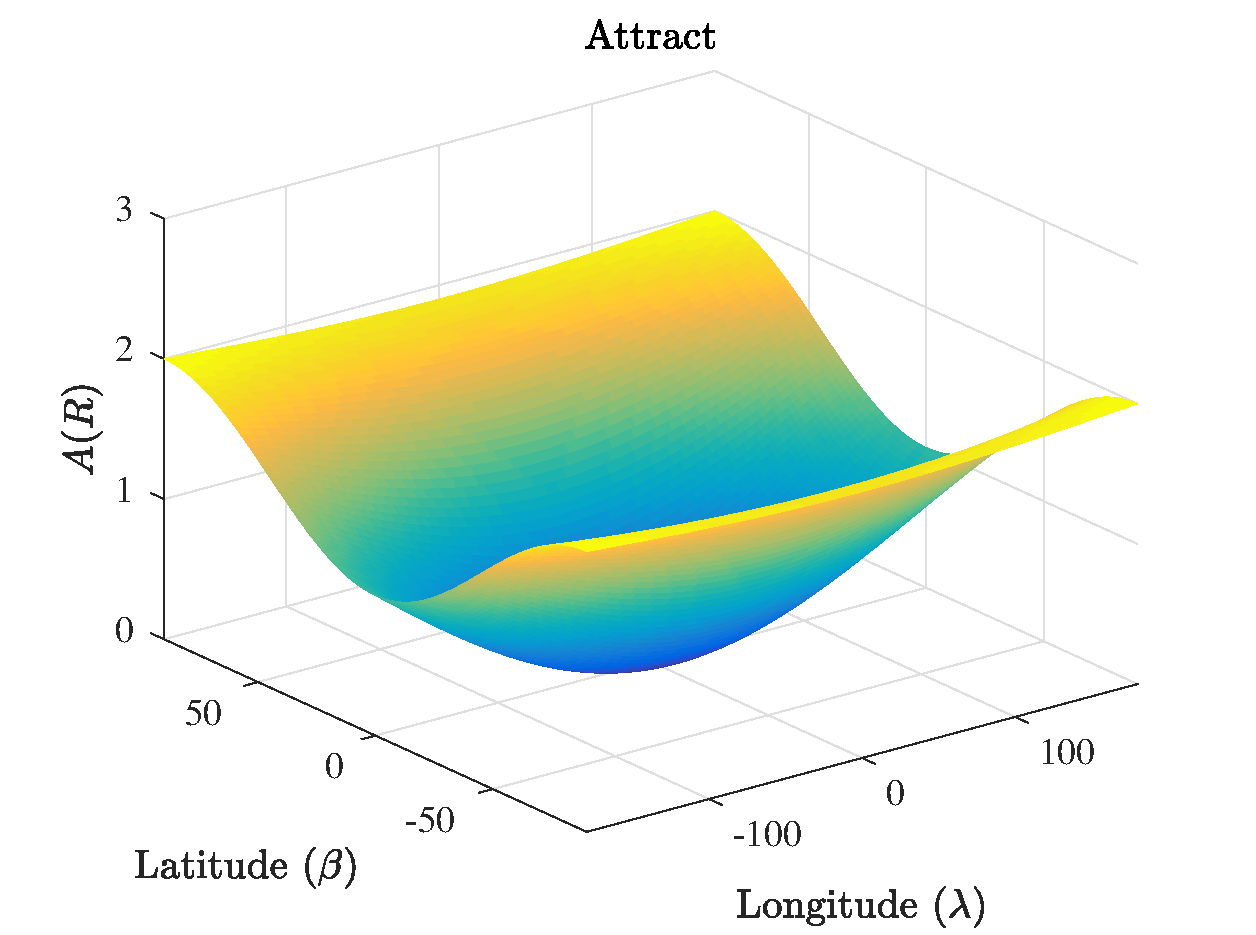
\includegraphics[trim={8mm 2mm 8mm 2mm}, clip]{figures/attract_error.pdf}}~
    \subfigure[Repulsive \( B(R) \) \label{fig:avoid_error} ]{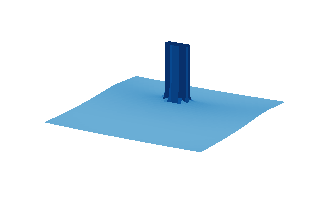
\includegraphics[trim={8mm 2mm 8mm 2mm}, clip]{figures/avoid_error.pdf}}~
    \subfigure[Combined \( \Psi \) \label{fig:combined_error}]{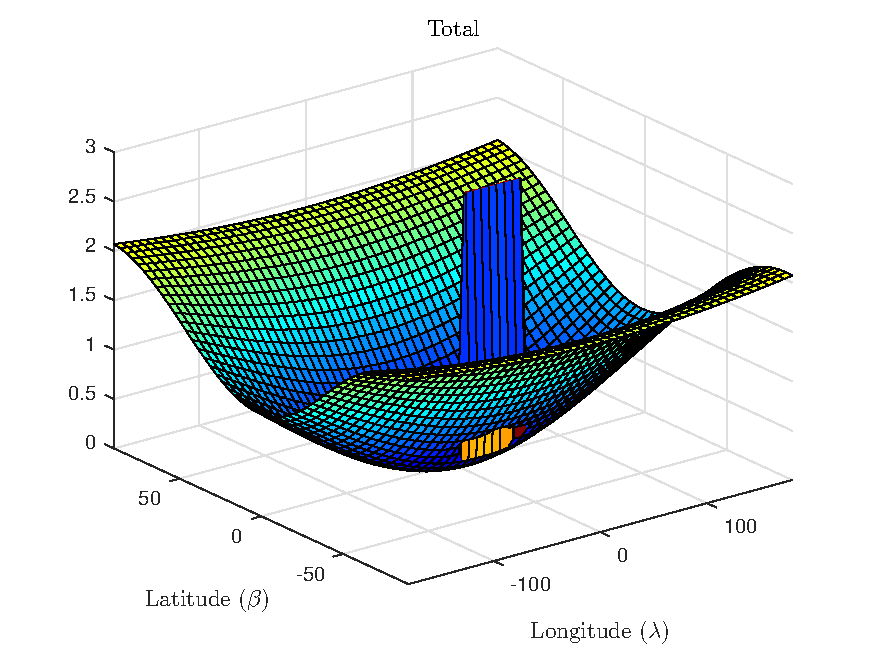
\includegraphics[trim={8mm 2mm 8mm 2mm}, clip]{figures/combined_error.pdf}}%
    \caption{Visualization of Configuration Error Functions using spherical coordinate representation}
    \label{fig:config_error} 
\end{figure}%
\begin{multicols}{2}
We apply this concept and parameterize the rotation matrix \( R \in \SO \) in terms of the spherical angles \( \SI{-180}{\degree} \leq \lambda \leq \SI{180}{\degree}  \) and \( \SI{-90}{\degree} \leq \beta \leq \SI{90}{\degree} \). 
Using the elementary Euler rotations, the rotation matrix is now defined as \( R = \exp( \lambda \hat{e}_2) \exp( \beta \hat{e}_3) \).
We iterate over the domains of \( \lambda\) and \(\beta\) in order to rotate the body-fixed vector \( r \) throughout the two-sphere \( \S^2 \).
Applying this method,~\cref{fig:config_error} allows us to visualize the error function on \( \SO \).
The horizontal axes of~\cref{fig:config_error} represent the domain of the spherical angles \( \lambda \) and \( \beta \) in degrees, while the vertical axes represent the unitless magnitude of the error functions defined in~\cref{eqn:psi,eqn:A,eqn:B}.
The attractive error function, given by~\cref{eqn:A}, has been previously used for attitude control on \(\SO\).
The potential well of \( A(R)\) is illustrated in~\cref{fig:attract_error}, where the desired attitude lies at the minimum of \( A(R) \).

To incorporate the state inequality constraints we apply a logarithmic barrier term.
Barrier functions are typically used in optimal control and motion planning applications.
A visualization of the repulsive error function is presented in~\cref{fig:avoid_error} which shows that as the boundary of the constraint is neared, or \( r^T R^T v \to \cos \theta \), the barrier term increases, \( B \to \infty\).
We use the scale factor~\(\frac{1}{1+\cos \theta} \) to ensure that \( \Psi \) remains positive definite.
The logarithmic function is popular as it quickly decays away from the constraint boundary.
The positive constant \( \alpha \) serves to shape the barrier function.
As \( \alpha \) is increased the impact of \( B(R) \) is reduced away from the constraint boundary. 
The superposition of the attractive and repulsive functions is shown in~\cref{fig:combined_error}.
The control system is defined such that the attitude trajectory follows the negative gradient of \( \Psi \) toward the minimum at \( R = R_d \), while avoiding the constrained region.

While~\cref{eqn:B} represents a single inequality constraint given as~\cref{eqn:constraint}, it is readily generalized to multiple constraints of an arbitrary orientation. 
For example, the configuration error function can be formulated as $\Psi=A[1+\sum_i C_i]$, where $C_i$ has the form of $C_i=B-1$ for the $i$-th constraint. 
In this manner, one may enforce multiple state inequality constraints, and we later demonstrate this through numerical simulation. 
This is in contrast to many previous approaches which are computationally difficult to extend to situations with multiple constraints.
We present the dynamics of the configuration error function in~\Cref{prop:error_dyn}, which are used in the subsequent development of the nonlinear control system.

\begin{prop}[Error Dynamics]\label{prop:error_dyn}
	The attitude error dynamics for \( \Psi, e_R, e_\Omega \) satisfy 
	\begin{gather}
		\diff{}{t} \parenth{\Psi} = e_R \cdot e_\Omega , \label{eqn:psi_dot}\\
		\diff{}{t} \parenth{e_R} = \dot{e}_{R_A} B + e_{R_A} \dot{B} + \dot{A}e_{R_B} + A \dot{e}_{R_B} , \label{eqn:eR_dot} \\
		\diff{}{t} \parenth{e_{R_A}} = E(R, R_d) e_\Omega , \label{eqn:eRA_dot} \\
		\diff{}{t} \parenth{e_{R_B}} = F(R) e_\Omega , \label{eqn:eRB_dot} \\
    	\diff{}{t} \parenth{A(R)} = e_{R_A} \cdot e_\Omega , \label{eqn:A_dot} \\
		\diff{}{t} \parenth{B(R)} = e_{R_B} \cdot e_\Omega , \label{eqn:B_dot} \\
		\diff{}{t} \parenth{e_\Omega} = J^{-1} \parenth{-\Omega \times J \Omega + u + W(R, \Omega) \Delta} , \label{eqn:eW_dot}
	\end{gather}
	where the matrices \(E(R,R_d), F(R) \in \R^{3\times3} \) are given by
	\begin{align}
		E(R,R_d) = &\frac{1}{2} \parenth{\tr{R^T R_d G}I - R^T R_d G} , \label{eqn:E} \\
		F(R) = &\frac{1}{\alpha \parenth{r^T R^T v - \cos \theta}} \left[\parenth{v^T R r} I - R^T v r^T + \right. \nonumber \\
		& \left. \frac{R^T \hat{v} R r v^T R \hat{r}}{\parenth{r^T R^T v - \cos \theta}}\right] . \label{eqn:F}
	\end{align}
\end{prop}
\begin{proof}
See~\Cref{proof:error_dyn}
\end{proof}

\end{multicols}
\begin{figure}[t]
    \centering 
    \subfigure[Attitude error vector \(e_R\) components \label{fig:eR_con}]{%% Creator: Matplotlib, PGF backend
%%
%% To include the figure in your LaTeX document, write
%%   \input{<filename>.pgf}
%%
%% Make sure the required packages are loaded in your preamble
%%   \usepackage{pgf}
%%
%% Figures using additional raster images can only be included by \input if
%% they are in the same directory as the main LaTeX file. For loading figures
%% from other directories you can use the `import` package
%%   \usepackage{import}
%% and then include the figures with
%%   \import{<path to file>}{<filename>.pgf}
%%
%% Matplotlib used the following preamble
%%   \usepackage[utf8x]{inputenc}
%%   \usepackage[T1]{fontenc}
%%   \usepackage{siunitx}
%%
\begingroup%
\makeatletter%
\begin{pgfpicture}%
\pgfpathrectangle{\pgfpointorigin}{\pgfqpoint{2.227534in}{1.887367in}}%
\pgfusepath{use as bounding box, clip}%
\begin{pgfscope}%
\pgfsetbuttcap%
\pgfsetmiterjoin%
\definecolor{currentfill}{rgb}{1.000000,1.000000,1.000000}%
\pgfsetfillcolor{currentfill}%
\pgfsetlinewidth{0.000000pt}%
\definecolor{currentstroke}{rgb}{1.000000,1.000000,1.000000}%
\pgfsetstrokecolor{currentstroke}%
\pgfsetdash{}{0pt}%
\pgfpathmoveto{\pgfqpoint{0.000000in}{0.000000in}}%
\pgfpathlineto{\pgfqpoint{2.227534in}{0.000000in}}%
\pgfpathlineto{\pgfqpoint{2.227534in}{1.887367in}}%
\pgfpathlineto{\pgfqpoint{0.000000in}{1.887367in}}%
\pgfpathclose%
\pgfusepath{fill}%
\end{pgfscope}%
\begin{pgfscope}%
\pgfsetbuttcap%
\pgfsetmiterjoin%
\definecolor{currentfill}{rgb}{1.000000,1.000000,1.000000}%
\pgfsetfillcolor{currentfill}%
\pgfsetlinewidth{0.000000pt}%
\definecolor{currentstroke}{rgb}{0.000000,0.000000,0.000000}%
\pgfsetstrokecolor{currentstroke}%
\pgfsetstrokeopacity{0.000000}%
\pgfsetdash{}{0pt}%
\pgfpathmoveto{\pgfqpoint{0.521753in}{1.456385in}}%
\pgfpathlineto{\pgfqpoint{2.107534in}{1.456385in}}%
\pgfpathlineto{\pgfqpoint{2.107534in}{1.742394in}}%
\pgfpathlineto{\pgfqpoint{0.521753in}{1.742394in}}%
\pgfpathclose%
\pgfusepath{fill}%
\end{pgfscope}%
\begin{pgfscope}%
\pgfpathrectangle{\pgfqpoint{0.521753in}{1.456385in}}{\pgfqpoint{1.585781in}{0.286009in}} %
\pgfusepath{clip}%
\pgfsetroundcap%
\pgfsetroundjoin%
\pgfsetlinewidth{1.003750pt}%
\definecolor{currentstroke}{rgb}{0.800000,0.800000,0.800000}%
\pgfsetstrokecolor{currentstroke}%
\pgfsetdash{}{0pt}%
\pgfpathmoveto{\pgfqpoint{0.593834in}{1.456385in}}%
\pgfpathlineto{\pgfqpoint{0.593834in}{1.742394in}}%
\pgfusepath{stroke}%
\end{pgfscope}%
\begin{pgfscope}%
\pgfpathrectangle{\pgfqpoint{0.521753in}{1.456385in}}{\pgfqpoint{1.585781in}{0.286009in}} %
\pgfusepath{clip}%
\pgfsetroundcap%
\pgfsetroundjoin%
\pgfsetlinewidth{1.003750pt}%
\definecolor{currentstroke}{rgb}{0.800000,0.800000,0.800000}%
\pgfsetstrokecolor{currentstroke}%
\pgfsetdash{}{0pt}%
\pgfpathmoveto{\pgfqpoint{1.314644in}{1.456385in}}%
\pgfpathlineto{\pgfqpoint{1.314644in}{1.742394in}}%
\pgfusepath{stroke}%
\end{pgfscope}%
\begin{pgfscope}%
\pgfpathrectangle{\pgfqpoint{0.521753in}{1.456385in}}{\pgfqpoint{1.585781in}{0.286009in}} %
\pgfusepath{clip}%
\pgfsetroundcap%
\pgfsetroundjoin%
\pgfsetlinewidth{1.003750pt}%
\definecolor{currentstroke}{rgb}{0.800000,0.800000,0.800000}%
\pgfsetstrokecolor{currentstroke}%
\pgfsetdash{}{0pt}%
\pgfpathmoveto{\pgfqpoint{2.035453in}{1.456385in}}%
\pgfpathlineto{\pgfqpoint{2.035453in}{1.742394in}}%
\pgfusepath{stroke}%
\end{pgfscope}%
\begin{pgfscope}%
\pgfpathrectangle{\pgfqpoint{0.521753in}{1.456385in}}{\pgfqpoint{1.585781in}{0.286009in}} %
\pgfusepath{clip}%
\pgfsetroundcap%
\pgfsetroundjoin%
\pgfsetlinewidth{1.003750pt}%
\definecolor{currentstroke}{rgb}{0.800000,0.800000,0.800000}%
\pgfsetstrokecolor{currentstroke}%
\pgfsetdash{}{0pt}%
\pgfpathmoveto{\pgfqpoint{0.521753in}{1.469385in}}%
\pgfpathlineto{\pgfqpoint{2.107534in}{1.469385in}}%
\pgfusepath{stroke}%
\end{pgfscope}%
\begin{pgfscope}%
\definecolor{textcolor}{rgb}{0.150000,0.150000,0.150000}%
\pgfsetstrokecolor{textcolor}%
\pgfsetfillcolor{textcolor}%
\pgftext[x=0.273680in,y=1.431123in,left,base]{\color{textcolor}\rmfamily\fontsize{8.000000}{9.600000}\selectfont \(\displaystyle 0.0\)}%
\end{pgfscope}%
\begin{pgfscope}%
\pgfpathrectangle{\pgfqpoint{0.521753in}{1.456385in}}{\pgfqpoint{1.585781in}{0.286009in}} %
\pgfusepath{clip}%
\pgfsetroundcap%
\pgfsetroundjoin%
\pgfsetlinewidth{1.003750pt}%
\definecolor{currentstroke}{rgb}{0.800000,0.800000,0.800000}%
\pgfsetstrokecolor{currentstroke}%
\pgfsetdash{}{0pt}%
\pgfpathmoveto{\pgfqpoint{0.521753in}{1.729422in}}%
\pgfpathlineto{\pgfqpoint{2.107534in}{1.729422in}}%
\pgfusepath{stroke}%
\end{pgfscope}%
\begin{pgfscope}%
\definecolor{textcolor}{rgb}{0.150000,0.150000,0.150000}%
\pgfsetstrokecolor{textcolor}%
\pgfsetfillcolor{textcolor}%
\pgftext[x=0.273680in,y=1.691160in,left,base]{\color{textcolor}\rmfamily\fontsize{8.000000}{9.600000}\selectfont \(\displaystyle 0.5\)}%
\end{pgfscope}%
\begin{pgfscope}%
\definecolor{textcolor}{rgb}{0.150000,0.150000,0.150000}%
\pgfsetstrokecolor{textcolor}%
\pgfsetfillcolor{textcolor}%
\pgftext[x=0.218124in,y=1.599389in,,bottom,rotate=90.000000]{\color{textcolor}\rmfamily\fontsize{8.000000}{9.600000}\selectfont \(\displaystyle e_{R_1}\)}%
\end{pgfscope}%
\begin{pgfscope}%
\pgfpathrectangle{\pgfqpoint{0.521753in}{1.456385in}}{\pgfqpoint{1.585781in}{0.286009in}} %
\pgfusepath{clip}%
\pgfsetroundcap%
\pgfsetroundjoin%
\pgfsetlinewidth{1.003750pt}%
\definecolor{currentstroke}{rgb}{0.298039,0.447059,0.690196}%
\pgfsetstrokecolor{currentstroke}%
\pgfsetdash{}{0pt}%
\pgfpathmoveto{\pgfqpoint{0.593834in}{1.469385in}}%
\pgfpathlineto{\pgfqpoint{0.596720in}{1.470885in}}%
\pgfpathlineto{\pgfqpoint{0.602492in}{1.478007in}}%
\pgfpathlineto{\pgfqpoint{0.612594in}{1.494787in}}%
\pgfpathlineto{\pgfqpoint{0.628468in}{1.522524in}}%
\pgfpathlineto{\pgfqpoint{0.663101in}{1.562706in}}%
\pgfpathlineto{\pgfqpoint{0.683304in}{1.581439in}}%
\pgfpathlineto{\pgfqpoint{0.702064in}{1.595742in}}%
\pgfpathlineto{\pgfqpoint{0.720824in}{1.607351in}}%
\pgfpathlineto{\pgfqpoint{0.739583in}{1.616436in}}%
\pgfpathlineto{\pgfqpoint{0.758343in}{1.623097in}}%
\pgfpathlineto{\pgfqpoint{0.777103in}{1.627341in}}%
\pgfpathlineto{\pgfqpoint{0.794420in}{1.629041in}}%
\pgfpathlineto{\pgfqpoint{0.811736in}{1.628471in}}%
\pgfpathlineto{\pgfqpoint{0.827610in}{1.625780in}}%
\pgfpathlineto{\pgfqpoint{0.843484in}{1.620793in}}%
\pgfpathlineto{\pgfqpoint{0.857914in}{1.614036in}}%
\pgfpathlineto{\pgfqpoint{0.872345in}{1.604884in}}%
\pgfpathlineto{\pgfqpoint{0.886776in}{1.592983in}}%
\pgfpathlineto{\pgfqpoint{0.899763in}{1.579546in}}%
\pgfpathlineto{\pgfqpoint{0.912751in}{1.563136in}}%
\pgfpathlineto{\pgfqpoint{0.927181in}{1.541131in}}%
\pgfpathlineto{\pgfqpoint{0.950270in}{1.500440in}}%
\pgfpathlineto{\pgfqpoint{0.961815in}{1.482817in}}%
\pgfpathlineto{\pgfqpoint{0.969030in}{1.475598in}}%
\pgfpathlineto{\pgfqpoint{0.974802in}{1.472877in}}%
\pgfpathlineto{\pgfqpoint{0.979132in}{1.472827in}}%
\pgfpathlineto{\pgfqpoint{0.984904in}{1.475391in}}%
\pgfpathlineto{\pgfqpoint{0.990676in}{1.480655in}}%
\pgfpathlineto{\pgfqpoint{0.997891in}{1.490220in}}%
\pgfpathlineto{\pgfqpoint{1.009436in}{1.509720in}}%
\pgfpathlineto{\pgfqpoint{1.045513in}{1.573556in}}%
\pgfpathlineto{\pgfqpoint{1.061386in}{1.596451in}}%
\pgfpathlineto{\pgfqpoint{1.077260in}{1.615572in}}%
\pgfpathlineto{\pgfqpoint{1.093134in}{1.631383in}}%
\pgfpathlineto{\pgfqpoint{1.110450in}{1.645518in}}%
\pgfpathlineto{\pgfqpoint{1.129210in}{1.657932in}}%
\pgfpathlineto{\pgfqpoint{1.150856in}{1.669415in}}%
\pgfpathlineto{\pgfqpoint{1.175388in}{1.679730in}}%
\pgfpathlineto{\pgfqpoint{1.204249in}{1.689261in}}%
\pgfpathlineto{\pgfqpoint{1.237440in}{1.697789in}}%
\pgfpathlineto{\pgfqpoint{1.276402in}{1.705479in}}%
\pgfpathlineto{\pgfqpoint{1.322580in}{1.712292in}}%
\pgfpathlineto{\pgfqpoint{1.377417in}{1.718059in}}%
\pgfpathlineto{\pgfqpoint{1.442355in}{1.722588in}}%
\pgfpathlineto{\pgfqpoint{1.523166in}{1.725915in}}%
\pgfpathlineto{\pgfqpoint{1.634282in}{1.728097in}}%
\pgfpathlineto{\pgfqpoint{1.818994in}{1.729186in}}%
\pgfpathlineto{\pgfqpoint{2.035453in}{1.729393in}}%
\pgfpathlineto{\pgfqpoint{2.035453in}{1.729393in}}%
\pgfusepath{stroke}%
\end{pgfscope}%
\begin{pgfscope}%
\pgfpathrectangle{\pgfqpoint{0.521753in}{1.456385in}}{\pgfqpoint{1.585781in}{0.286009in}} %
\pgfusepath{clip}%
\pgfsetbuttcap%
\pgfsetroundjoin%
\pgfsetlinewidth{1.003750pt}%
\definecolor{currentstroke}{rgb}{0.333333,0.658824,0.407843}%
\pgfsetstrokecolor{currentstroke}%
\pgfsetdash{{5.600000pt}{2.400000pt}}{0.000000pt}%
\pgfpathmoveto{\pgfqpoint{0.593834in}{1.469385in}}%
\pgfpathlineto{\pgfqpoint{2.035453in}{1.469385in}}%
\pgfpathlineto{\pgfqpoint{2.035453in}{1.469385in}}%
\pgfusepath{stroke}%
\end{pgfscope}%
\begin{pgfscope}%
\pgfsetrectcap%
\pgfsetmiterjoin%
\pgfsetlinewidth{1.003750pt}%
\definecolor{currentstroke}{rgb}{0.800000,0.800000,0.800000}%
\pgfsetstrokecolor{currentstroke}%
\pgfsetdash{}{0pt}%
\pgfpathmoveto{\pgfqpoint{0.521753in}{1.456385in}}%
\pgfpathlineto{\pgfqpoint{0.521753in}{1.742394in}}%
\pgfusepath{stroke}%
\end{pgfscope}%
\begin{pgfscope}%
\pgfsetrectcap%
\pgfsetmiterjoin%
\pgfsetlinewidth{1.003750pt}%
\definecolor{currentstroke}{rgb}{0.800000,0.800000,0.800000}%
\pgfsetstrokecolor{currentstroke}%
\pgfsetdash{}{0pt}%
\pgfpathmoveto{\pgfqpoint{2.107534in}{1.456385in}}%
\pgfpathlineto{\pgfqpoint{2.107534in}{1.742394in}}%
\pgfusepath{stroke}%
\end{pgfscope}%
\begin{pgfscope}%
\pgfsetrectcap%
\pgfsetmiterjoin%
\pgfsetlinewidth{1.003750pt}%
\definecolor{currentstroke}{rgb}{0.800000,0.800000,0.800000}%
\pgfsetstrokecolor{currentstroke}%
\pgfsetdash{}{0pt}%
\pgfpathmoveto{\pgfqpoint{0.521753in}{1.456385in}}%
\pgfpathlineto{\pgfqpoint{2.107534in}{1.456385in}}%
\pgfusepath{stroke}%
\end{pgfscope}%
\begin{pgfscope}%
\pgfsetrectcap%
\pgfsetmiterjoin%
\pgfsetlinewidth{1.003750pt}%
\definecolor{currentstroke}{rgb}{0.800000,0.800000,0.800000}%
\pgfsetstrokecolor{currentstroke}%
\pgfsetdash{}{0pt}%
\pgfpathmoveto{\pgfqpoint{0.521753in}{1.742394in}}%
\pgfpathlineto{\pgfqpoint{2.107534in}{1.742394in}}%
\pgfusepath{stroke}%
\end{pgfscope}%
\begin{pgfscope}%
\pgfsetbuttcap%
\pgfsetmiterjoin%
\definecolor{currentfill}{rgb}{1.000000,1.000000,1.000000}%
\pgfsetfillcolor{currentfill}%
\pgfsetlinewidth{0.000000pt}%
\definecolor{currentstroke}{rgb}{0.000000,0.000000,0.000000}%
\pgfsetstrokecolor{currentstroke}%
\pgfsetstrokeopacity{0.000000}%
\pgfsetdash{}{0pt}%
\pgfpathmoveto{\pgfqpoint{0.521753in}{0.969185in}}%
\pgfpathlineto{\pgfqpoint{2.107534in}{0.969185in}}%
\pgfpathlineto{\pgfqpoint{2.107534in}{1.255195in}}%
\pgfpathlineto{\pgfqpoint{0.521753in}{1.255195in}}%
\pgfpathclose%
\pgfusepath{fill}%
\end{pgfscope}%
\begin{pgfscope}%
\pgfpathrectangle{\pgfqpoint{0.521753in}{0.969185in}}{\pgfqpoint{1.585781in}{0.286009in}} %
\pgfusepath{clip}%
\pgfsetroundcap%
\pgfsetroundjoin%
\pgfsetlinewidth{1.003750pt}%
\definecolor{currentstroke}{rgb}{0.800000,0.800000,0.800000}%
\pgfsetstrokecolor{currentstroke}%
\pgfsetdash{}{0pt}%
\pgfpathmoveto{\pgfqpoint{0.593834in}{0.969185in}}%
\pgfpathlineto{\pgfqpoint{0.593834in}{1.255195in}}%
\pgfusepath{stroke}%
\end{pgfscope}%
\begin{pgfscope}%
\pgfpathrectangle{\pgfqpoint{0.521753in}{0.969185in}}{\pgfqpoint{1.585781in}{0.286009in}} %
\pgfusepath{clip}%
\pgfsetroundcap%
\pgfsetroundjoin%
\pgfsetlinewidth{1.003750pt}%
\definecolor{currentstroke}{rgb}{0.800000,0.800000,0.800000}%
\pgfsetstrokecolor{currentstroke}%
\pgfsetdash{}{0pt}%
\pgfpathmoveto{\pgfqpoint{1.314644in}{0.969185in}}%
\pgfpathlineto{\pgfqpoint{1.314644in}{1.255195in}}%
\pgfusepath{stroke}%
\end{pgfscope}%
\begin{pgfscope}%
\pgfpathrectangle{\pgfqpoint{0.521753in}{0.969185in}}{\pgfqpoint{1.585781in}{0.286009in}} %
\pgfusepath{clip}%
\pgfsetroundcap%
\pgfsetroundjoin%
\pgfsetlinewidth{1.003750pt}%
\definecolor{currentstroke}{rgb}{0.800000,0.800000,0.800000}%
\pgfsetstrokecolor{currentstroke}%
\pgfsetdash{}{0pt}%
\pgfpathmoveto{\pgfqpoint{2.035453in}{0.969185in}}%
\pgfpathlineto{\pgfqpoint{2.035453in}{1.255195in}}%
\pgfusepath{stroke}%
\end{pgfscope}%
\begin{pgfscope}%
\pgfpathrectangle{\pgfqpoint{0.521753in}{0.969185in}}{\pgfqpoint{1.585781in}{0.286009in}} %
\pgfusepath{clip}%
\pgfsetroundcap%
\pgfsetroundjoin%
\pgfsetlinewidth{1.003750pt}%
\definecolor{currentstroke}{rgb}{0.800000,0.800000,0.800000}%
\pgfsetstrokecolor{currentstroke}%
\pgfsetdash{}{0pt}%
\pgfpathmoveto{\pgfqpoint{0.521753in}{1.099279in}}%
\pgfpathlineto{\pgfqpoint{2.107534in}{1.099279in}}%
\pgfusepath{stroke}%
\end{pgfscope}%
\begin{pgfscope}%
\definecolor{textcolor}{rgb}{0.150000,0.150000,0.150000}%
\pgfsetstrokecolor{textcolor}%
\pgfsetfillcolor{textcolor}%
\pgftext[x=0.365502in,y=1.061016in,left,base]{\color{textcolor}\rmfamily\fontsize{8.000000}{9.600000}\selectfont \(\displaystyle 0\)}%
\end{pgfscope}%
\begin{pgfscope}%
\pgfpathrectangle{\pgfqpoint{0.521753in}{0.969185in}}{\pgfqpoint{1.585781in}{0.286009in}} %
\pgfusepath{clip}%
\pgfsetroundcap%
\pgfsetroundjoin%
\pgfsetlinewidth{1.003750pt}%
\definecolor{currentstroke}{rgb}{0.800000,0.800000,0.800000}%
\pgfsetstrokecolor{currentstroke}%
\pgfsetdash{}{0pt}%
\pgfpathmoveto{\pgfqpoint{0.521753in}{1.251666in}}%
\pgfpathlineto{\pgfqpoint{2.107534in}{1.251666in}}%
\pgfusepath{stroke}%
\end{pgfscope}%
\begin{pgfscope}%
\definecolor{textcolor}{rgb}{0.150000,0.150000,0.150000}%
\pgfsetstrokecolor{textcolor}%
\pgfsetfillcolor{textcolor}%
\pgftext[x=0.365502in,y=1.213404in,left,base]{\color{textcolor}\rmfamily\fontsize{8.000000}{9.600000}\selectfont \(\displaystyle 1\)}%
\end{pgfscope}%
\begin{pgfscope}%
\definecolor{textcolor}{rgb}{0.150000,0.150000,0.150000}%
\pgfsetstrokecolor{textcolor}%
\pgfsetfillcolor{textcolor}%
\pgftext[x=0.309947in,y=1.112190in,,bottom,rotate=90.000000]{\color{textcolor}\rmfamily\fontsize{8.000000}{9.600000}\selectfont \(\displaystyle e_{R_2}\)}%
\end{pgfscope}%
\begin{pgfscope}%
\pgfpathrectangle{\pgfqpoint{0.521753in}{0.969185in}}{\pgfqpoint{1.585781in}{0.286009in}} %
\pgfusepath{clip}%
\pgfsetroundcap%
\pgfsetroundjoin%
\pgfsetlinewidth{1.003750pt}%
\definecolor{currentstroke}{rgb}{0.298039,0.447059,0.690196}%
\pgfsetstrokecolor{currentstroke}%
\pgfsetdash{}{0pt}%
\pgfpathmoveto{\pgfqpoint{0.593834in}{1.126430in}}%
\pgfpathlineto{\pgfqpoint{0.611151in}{1.126569in}}%
\pgfpathlineto{\pgfqpoint{0.615480in}{1.129466in}}%
\pgfpathlineto{\pgfqpoint{0.619809in}{1.135878in}}%
\pgfpathlineto{\pgfqpoint{0.627024in}{1.149314in}}%
\pgfpathlineto{\pgfqpoint{0.629911in}{1.148753in}}%
\pgfpathlineto{\pgfqpoint{0.637126in}{1.144530in}}%
\pgfpathlineto{\pgfqpoint{0.641455in}{1.144763in}}%
\pgfpathlineto{\pgfqpoint{0.651557in}{1.149018in}}%
\pgfpathlineto{\pgfqpoint{0.660215in}{1.151304in}}%
\pgfpathlineto{\pgfqpoint{0.683304in}{1.156386in}}%
\pgfpathlineto{\pgfqpoint{0.749685in}{1.172931in}}%
\pgfpathlineto{\pgfqpoint{0.779989in}{1.182931in}}%
\pgfpathlineto{\pgfqpoint{0.805964in}{1.193860in}}%
\pgfpathlineto{\pgfqpoint{0.830496in}{1.206704in}}%
\pgfpathlineto{\pgfqpoint{0.862244in}{1.226275in}}%
\pgfpathlineto{\pgfqpoint{0.882446in}{1.237681in}}%
\pgfpathlineto{\pgfqpoint{0.893991in}{1.241615in}}%
\pgfpathlineto{\pgfqpoint{0.902649in}{1.242008in}}%
\pgfpathlineto{\pgfqpoint{0.909865in}{1.239787in}}%
\pgfpathlineto{\pgfqpoint{0.915637in}{1.235772in}}%
\pgfpathlineto{\pgfqpoint{0.921409in}{1.229254in}}%
\pgfpathlineto{\pgfqpoint{0.927181in}{1.219719in}}%
\pgfpathlineto{\pgfqpoint{0.934397in}{1.202780in}}%
\pgfpathlineto{\pgfqpoint{0.941612in}{1.179518in}}%
\pgfpathlineto{\pgfqpoint{0.950270in}{1.143038in}}%
\pgfpathlineto{\pgfqpoint{0.964701in}{1.068783in}}%
\pgfpathlineto{\pgfqpoint{0.974802in}{1.021623in}}%
\pgfpathlineto{\pgfqpoint{0.982018in}{0.998428in}}%
\pgfpathlineto{\pgfqpoint{0.987790in}{0.987511in}}%
\pgfpathlineto{\pgfqpoint{0.992119in}{0.983399in}}%
\pgfpathlineto{\pgfqpoint{0.996448in}{0.982186in}}%
\pgfpathlineto{\pgfqpoint{1.000778in}{0.983274in}}%
\pgfpathlineto{\pgfqpoint{1.006550in}{0.987352in}}%
\pgfpathlineto{\pgfqpoint{1.015208in}{0.997018in}}%
\pgfpathlineto{\pgfqpoint{1.031082in}{1.019293in}}%
\pgfpathlineto{\pgfqpoint{1.057057in}{1.055320in}}%
\pgfpathlineto{\pgfqpoint{1.074374in}{1.075626in}}%
\pgfpathlineto{\pgfqpoint{1.091691in}{1.092601in}}%
\pgfpathlineto{\pgfqpoint{1.109007in}{1.106609in}}%
\pgfpathlineto{\pgfqpoint{1.127767in}{1.119000in}}%
\pgfpathlineto{\pgfqpoint{1.147970in}{1.129748in}}%
\pgfpathlineto{\pgfqpoint{1.171059in}{1.139459in}}%
\pgfpathlineto{\pgfqpoint{1.197034in}{1.147883in}}%
\pgfpathlineto{\pgfqpoint{1.227338in}{1.155226in}}%
\pgfpathlineto{\pgfqpoint{1.261972in}{1.161254in}}%
\pgfpathlineto{\pgfqpoint{1.303821in}{1.166208in}}%
\pgfpathlineto{\pgfqpoint{1.355771in}{1.170046in}}%
\pgfpathlineto{\pgfqpoint{1.425038in}{1.172829in}}%
\pgfpathlineto{\pgfqpoint{1.528938in}{1.174580in}}%
\pgfpathlineto{\pgfqpoint{1.732410in}{1.175361in}}%
\pgfpathlineto{\pgfqpoint{2.035453in}{1.175466in}}%
\pgfpathlineto{\pgfqpoint{2.035453in}{1.175466in}}%
\pgfusepath{stroke}%
\end{pgfscope}%
\begin{pgfscope}%
\pgfpathrectangle{\pgfqpoint{0.521753in}{0.969185in}}{\pgfqpoint{1.585781in}{0.286009in}} %
\pgfusepath{clip}%
\pgfsetbuttcap%
\pgfsetroundjoin%
\pgfsetlinewidth{1.003750pt}%
\definecolor{currentstroke}{rgb}{0.333333,0.658824,0.407843}%
\pgfsetstrokecolor{currentstroke}%
\pgfsetdash{{5.600000pt}{2.400000pt}}{0.000000pt}%
\pgfpathmoveto{\pgfqpoint{0.593834in}{1.099279in}}%
\pgfpathlineto{\pgfqpoint{2.035453in}{1.099279in}}%
\pgfpathlineto{\pgfqpoint{2.035453in}{1.099279in}}%
\pgfusepath{stroke}%
\end{pgfscope}%
\begin{pgfscope}%
\pgfsetrectcap%
\pgfsetmiterjoin%
\pgfsetlinewidth{1.003750pt}%
\definecolor{currentstroke}{rgb}{0.800000,0.800000,0.800000}%
\pgfsetstrokecolor{currentstroke}%
\pgfsetdash{}{0pt}%
\pgfpathmoveto{\pgfqpoint{0.521753in}{0.969185in}}%
\pgfpathlineto{\pgfqpoint{0.521753in}{1.255195in}}%
\pgfusepath{stroke}%
\end{pgfscope}%
\begin{pgfscope}%
\pgfsetrectcap%
\pgfsetmiterjoin%
\pgfsetlinewidth{1.003750pt}%
\definecolor{currentstroke}{rgb}{0.800000,0.800000,0.800000}%
\pgfsetstrokecolor{currentstroke}%
\pgfsetdash{}{0pt}%
\pgfpathmoveto{\pgfqpoint{2.107534in}{0.969185in}}%
\pgfpathlineto{\pgfqpoint{2.107534in}{1.255195in}}%
\pgfusepath{stroke}%
\end{pgfscope}%
\begin{pgfscope}%
\pgfsetrectcap%
\pgfsetmiterjoin%
\pgfsetlinewidth{1.003750pt}%
\definecolor{currentstroke}{rgb}{0.800000,0.800000,0.800000}%
\pgfsetstrokecolor{currentstroke}%
\pgfsetdash{}{0pt}%
\pgfpathmoveto{\pgfqpoint{0.521753in}{0.969185in}}%
\pgfpathlineto{\pgfqpoint{2.107534in}{0.969185in}}%
\pgfusepath{stroke}%
\end{pgfscope}%
\begin{pgfscope}%
\pgfsetrectcap%
\pgfsetmiterjoin%
\pgfsetlinewidth{1.003750pt}%
\definecolor{currentstroke}{rgb}{0.800000,0.800000,0.800000}%
\pgfsetstrokecolor{currentstroke}%
\pgfsetdash{}{0pt}%
\pgfpathmoveto{\pgfqpoint{0.521753in}{1.255195in}}%
\pgfpathlineto{\pgfqpoint{2.107534in}{1.255195in}}%
\pgfusepath{stroke}%
\end{pgfscope}%
\begin{pgfscope}%
\pgfsetbuttcap%
\pgfsetmiterjoin%
\definecolor{currentfill}{rgb}{1.000000,1.000000,1.000000}%
\pgfsetfillcolor{currentfill}%
\pgfsetlinewidth{0.000000pt}%
\definecolor{currentstroke}{rgb}{0.000000,0.000000,0.000000}%
\pgfsetstrokecolor{currentstroke}%
\pgfsetstrokeopacity{0.000000}%
\pgfsetdash{}{0pt}%
\pgfpathmoveto{\pgfqpoint{0.521753in}{0.481986in}}%
\pgfpathlineto{\pgfqpoint{2.107534in}{0.481986in}}%
\pgfpathlineto{\pgfqpoint{2.107534in}{0.767995in}}%
\pgfpathlineto{\pgfqpoint{0.521753in}{0.767995in}}%
\pgfpathclose%
\pgfusepath{fill}%
\end{pgfscope}%
\begin{pgfscope}%
\pgfpathrectangle{\pgfqpoint{0.521753in}{0.481986in}}{\pgfqpoint{1.585781in}{0.286009in}} %
\pgfusepath{clip}%
\pgfsetroundcap%
\pgfsetroundjoin%
\pgfsetlinewidth{1.003750pt}%
\definecolor{currentstroke}{rgb}{0.800000,0.800000,0.800000}%
\pgfsetstrokecolor{currentstroke}%
\pgfsetdash{}{0pt}%
\pgfpathmoveto{\pgfqpoint{0.593834in}{0.481986in}}%
\pgfpathlineto{\pgfqpoint{0.593834in}{0.767995in}}%
\pgfusepath{stroke}%
\end{pgfscope}%
\begin{pgfscope}%
\definecolor{textcolor}{rgb}{0.150000,0.150000,0.150000}%
\pgfsetstrokecolor{textcolor}%
\pgfsetfillcolor{textcolor}%
\pgftext[x=0.593834in,y=0.384764in,,top]{\color{textcolor}\rmfamily\fontsize{8.000000}{9.600000}\selectfont \(\displaystyle 0\)}%
\end{pgfscope}%
\begin{pgfscope}%
\pgfpathrectangle{\pgfqpoint{0.521753in}{0.481986in}}{\pgfqpoint{1.585781in}{0.286009in}} %
\pgfusepath{clip}%
\pgfsetroundcap%
\pgfsetroundjoin%
\pgfsetlinewidth{1.003750pt}%
\definecolor{currentstroke}{rgb}{0.800000,0.800000,0.800000}%
\pgfsetstrokecolor{currentstroke}%
\pgfsetdash{}{0pt}%
\pgfpathmoveto{\pgfqpoint{1.314644in}{0.481986in}}%
\pgfpathlineto{\pgfqpoint{1.314644in}{0.767995in}}%
\pgfusepath{stroke}%
\end{pgfscope}%
\begin{pgfscope}%
\definecolor{textcolor}{rgb}{0.150000,0.150000,0.150000}%
\pgfsetstrokecolor{textcolor}%
\pgfsetfillcolor{textcolor}%
\pgftext[x=1.314644in,y=0.384764in,,top]{\color{textcolor}\rmfamily\fontsize{8.000000}{9.600000}\selectfont \(\displaystyle 5\)}%
\end{pgfscope}%
\begin{pgfscope}%
\pgfpathrectangle{\pgfqpoint{0.521753in}{0.481986in}}{\pgfqpoint{1.585781in}{0.286009in}} %
\pgfusepath{clip}%
\pgfsetroundcap%
\pgfsetroundjoin%
\pgfsetlinewidth{1.003750pt}%
\definecolor{currentstroke}{rgb}{0.800000,0.800000,0.800000}%
\pgfsetstrokecolor{currentstroke}%
\pgfsetdash{}{0pt}%
\pgfpathmoveto{\pgfqpoint{2.035453in}{0.481986in}}%
\pgfpathlineto{\pgfqpoint{2.035453in}{0.767995in}}%
\pgfusepath{stroke}%
\end{pgfscope}%
\begin{pgfscope}%
\definecolor{textcolor}{rgb}{0.150000,0.150000,0.150000}%
\pgfsetstrokecolor{textcolor}%
\pgfsetfillcolor{textcolor}%
\pgftext[x=2.035453in,y=0.384764in,,top]{\color{textcolor}\rmfamily\fontsize{8.000000}{9.600000}\selectfont \(\displaystyle 10\)}%
\end{pgfscope}%
\begin{pgfscope}%
\definecolor{textcolor}{rgb}{0.150000,0.150000,0.150000}%
\pgfsetstrokecolor{textcolor}%
\pgfsetfillcolor{textcolor}%
\pgftext[x=1.314644in,y=0.231084in,,top]{\color{textcolor}\rmfamily\fontsize{8.000000}{9.600000}\selectfont \(\displaystyle t\) (sec)}%
\end{pgfscope}%
\begin{pgfscope}%
\pgfpathrectangle{\pgfqpoint{0.521753in}{0.481986in}}{\pgfqpoint{1.585781in}{0.286009in}} %
\pgfusepath{clip}%
\pgfsetroundcap%
\pgfsetroundjoin%
\pgfsetlinewidth{1.003750pt}%
\definecolor{currentstroke}{rgb}{0.800000,0.800000,0.800000}%
\pgfsetstrokecolor{currentstroke}%
\pgfsetdash{}{0pt}%
\pgfpathmoveto{\pgfqpoint{0.521753in}{0.525747in}}%
\pgfpathlineto{\pgfqpoint{2.107534in}{0.525747in}}%
\pgfusepath{stroke}%
\end{pgfscope}%
\begin{pgfscope}%
\definecolor{textcolor}{rgb}{0.150000,0.150000,0.150000}%
\pgfsetstrokecolor{textcolor}%
\pgfsetfillcolor{textcolor}%
\pgftext[x=0.273680in,y=0.487484in,left,base]{\color{textcolor}\rmfamily\fontsize{8.000000}{9.600000}\selectfont \(\displaystyle -1\)}%
\end{pgfscope}%
\begin{pgfscope}%
\pgfpathrectangle{\pgfqpoint{0.521753in}{0.481986in}}{\pgfqpoint{1.585781in}{0.286009in}} %
\pgfusepath{clip}%
\pgfsetroundcap%
\pgfsetroundjoin%
\pgfsetlinewidth{1.003750pt}%
\definecolor{currentstroke}{rgb}{0.800000,0.800000,0.800000}%
\pgfsetstrokecolor{currentstroke}%
\pgfsetdash{}{0pt}%
\pgfpathmoveto{\pgfqpoint{0.521753in}{0.645388in}}%
\pgfpathlineto{\pgfqpoint{2.107534in}{0.645388in}}%
\pgfusepath{stroke}%
\end{pgfscope}%
\begin{pgfscope}%
\definecolor{textcolor}{rgb}{0.150000,0.150000,0.150000}%
\pgfsetstrokecolor{textcolor}%
\pgfsetfillcolor{textcolor}%
\pgftext[x=0.365502in,y=0.607125in,left,base]{\color{textcolor}\rmfamily\fontsize{8.000000}{9.600000}\selectfont \(\displaystyle 0\)}%
\end{pgfscope}%
\begin{pgfscope}%
\pgfpathrectangle{\pgfqpoint{0.521753in}{0.481986in}}{\pgfqpoint{1.585781in}{0.286009in}} %
\pgfusepath{clip}%
\pgfsetroundcap%
\pgfsetroundjoin%
\pgfsetlinewidth{1.003750pt}%
\definecolor{currentstroke}{rgb}{0.800000,0.800000,0.800000}%
\pgfsetstrokecolor{currentstroke}%
\pgfsetdash{}{0pt}%
\pgfpathmoveto{\pgfqpoint{0.521753in}{0.765029in}}%
\pgfpathlineto{\pgfqpoint{2.107534in}{0.765029in}}%
\pgfusepath{stroke}%
\end{pgfscope}%
\begin{pgfscope}%
\definecolor{textcolor}{rgb}{0.150000,0.150000,0.150000}%
\pgfsetstrokecolor{textcolor}%
\pgfsetfillcolor{textcolor}%
\pgftext[x=0.365502in,y=0.726767in,left,base]{\color{textcolor}\rmfamily\fontsize{8.000000}{9.600000}\selectfont \(\displaystyle 1\)}%
\end{pgfscope}%
\begin{pgfscope}%
\definecolor{textcolor}{rgb}{0.150000,0.150000,0.150000}%
\pgfsetstrokecolor{textcolor}%
\pgfsetfillcolor{textcolor}%
\pgftext[x=0.218124in,y=0.624991in,,bottom,rotate=90.000000]{\color{textcolor}\rmfamily\fontsize{8.000000}{9.600000}\selectfont \(\displaystyle e_{R_3}\)}%
\end{pgfscope}%
\begin{pgfscope}%
\pgfpathrectangle{\pgfqpoint{0.521753in}{0.481986in}}{\pgfqpoint{1.585781in}{0.286009in}} %
\pgfusepath{clip}%
\pgfsetroundcap%
\pgfsetroundjoin%
\pgfsetlinewidth{1.003750pt}%
\definecolor{currentstroke}{rgb}{0.298039,0.447059,0.690196}%
\pgfsetstrokecolor{currentstroke}%
\pgfsetdash{}{0pt}%
\pgfpathmoveto{\pgfqpoint{0.593834in}{0.566867in}}%
\pgfpathlineto{\pgfqpoint{0.598163in}{0.568201in}}%
\pgfpathlineto{\pgfqpoint{0.602492in}{0.572347in}}%
\pgfpathlineto{\pgfqpoint{0.606822in}{0.580501in}}%
\pgfpathlineto{\pgfqpoint{0.611151in}{0.595457in}}%
\pgfpathlineto{\pgfqpoint{0.615480in}{0.622942in}}%
\pgfpathlineto{\pgfqpoint{0.619809in}{0.672088in}}%
\pgfpathlineto{\pgfqpoint{0.625581in}{0.749811in}}%
\pgfpathlineto{\pgfqpoint{0.627024in}{0.754995in}}%
\pgfpathlineto{\pgfqpoint{0.628468in}{0.752015in}}%
\pgfpathlineto{\pgfqpoint{0.637126in}{0.703455in}}%
\pgfpathlineto{\pgfqpoint{0.640012in}{0.699133in}}%
\pgfpathlineto{\pgfqpoint{0.642898in}{0.699588in}}%
\pgfpathlineto{\pgfqpoint{0.648670in}{0.706299in}}%
\pgfpathlineto{\pgfqpoint{0.653000in}{0.710114in}}%
\pgfpathlineto{\pgfqpoint{0.657329in}{0.710762in}}%
\pgfpathlineto{\pgfqpoint{0.674646in}{0.708156in}}%
\pgfpathlineto{\pgfqpoint{0.693405in}{0.708265in}}%
\pgfpathlineto{\pgfqpoint{0.761229in}{0.704998in}}%
\pgfpathlineto{\pgfqpoint{0.791534in}{0.701187in}}%
\pgfpathlineto{\pgfqpoint{0.813179in}{0.696412in}}%
\pgfpathlineto{\pgfqpoint{0.830496in}{0.690485in}}%
\pgfpathlineto{\pgfqpoint{0.844927in}{0.683379in}}%
\pgfpathlineto{\pgfqpoint{0.857914in}{0.674619in}}%
\pgfpathlineto{\pgfqpoint{0.869459in}{0.664345in}}%
\pgfpathlineto{\pgfqpoint{0.881003in}{0.651106in}}%
\pgfpathlineto{\pgfqpoint{0.892548in}{0.634270in}}%
\pgfpathlineto{\pgfqpoint{0.904092in}{0.613313in}}%
\pgfpathlineto{\pgfqpoint{0.917080in}{0.584680in}}%
\pgfpathlineto{\pgfqpoint{0.951713in}{0.503546in}}%
\pgfpathlineto{\pgfqpoint{0.957486in}{0.496942in}}%
\pgfpathlineto{\pgfqpoint{0.961815in}{0.495004in}}%
\pgfpathlineto{\pgfqpoint{0.966144in}{0.495910in}}%
\pgfpathlineto{\pgfqpoint{0.970473in}{0.499618in}}%
\pgfpathlineto{\pgfqpoint{0.976246in}{0.508312in}}%
\pgfpathlineto{\pgfqpoint{0.984904in}{0.526424in}}%
\pgfpathlineto{\pgfqpoint{1.005107in}{0.569969in}}%
\pgfpathlineto{\pgfqpoint{1.018094in}{0.592006in}}%
\pgfpathlineto{\pgfqpoint{1.032525in}{0.611837in}}%
\pgfpathlineto{\pgfqpoint{1.048399in}{0.629659in}}%
\pgfpathlineto{\pgfqpoint{1.064272in}{0.644290in}}%
\pgfpathlineto{\pgfqpoint{1.081589in}{0.657242in}}%
\pgfpathlineto{\pgfqpoint{1.098906in}{0.667543in}}%
\pgfpathlineto{\pgfqpoint{1.117666in}{0.676236in}}%
\pgfpathlineto{\pgfqpoint{1.139312in}{0.683753in}}%
\pgfpathlineto{\pgfqpoint{1.163844in}{0.689853in}}%
\pgfpathlineto{\pgfqpoint{1.194148in}{0.694931in}}%
\pgfpathlineto{\pgfqpoint{1.231668in}{0.698826in}}%
\pgfpathlineto{\pgfqpoint{1.282175in}{0.701711in}}%
\pgfpathlineto{\pgfqpoint{1.360100in}{0.703690in}}%
\pgfpathlineto{\pgfqpoint{1.507292in}{0.704800in}}%
\pgfpathlineto{\pgfqpoint{1.963300in}{0.705198in}}%
\pgfpathlineto{\pgfqpoint{2.035453in}{0.705203in}}%
\pgfpathlineto{\pgfqpoint{2.035453in}{0.705203in}}%
\pgfusepath{stroke}%
\end{pgfscope}%
\begin{pgfscope}%
\pgfpathrectangle{\pgfqpoint{0.521753in}{0.481986in}}{\pgfqpoint{1.585781in}{0.286009in}} %
\pgfusepath{clip}%
\pgfsetbuttcap%
\pgfsetroundjoin%
\pgfsetlinewidth{1.003750pt}%
\definecolor{currentstroke}{rgb}{0.333333,0.658824,0.407843}%
\pgfsetstrokecolor{currentstroke}%
\pgfsetdash{{5.600000pt}{2.400000pt}}{0.000000pt}%
\pgfpathmoveto{\pgfqpoint{0.593834in}{0.645388in}}%
\pgfpathlineto{\pgfqpoint{2.035453in}{0.645388in}}%
\pgfpathlineto{\pgfqpoint{2.035453in}{0.645388in}}%
\pgfusepath{stroke}%
\end{pgfscope}%
\begin{pgfscope}%
\pgfsetrectcap%
\pgfsetmiterjoin%
\pgfsetlinewidth{1.003750pt}%
\definecolor{currentstroke}{rgb}{0.800000,0.800000,0.800000}%
\pgfsetstrokecolor{currentstroke}%
\pgfsetdash{}{0pt}%
\pgfpathmoveto{\pgfqpoint{0.521753in}{0.481986in}}%
\pgfpathlineto{\pgfqpoint{0.521753in}{0.767995in}}%
\pgfusepath{stroke}%
\end{pgfscope}%
\begin{pgfscope}%
\pgfsetrectcap%
\pgfsetmiterjoin%
\pgfsetlinewidth{1.003750pt}%
\definecolor{currentstroke}{rgb}{0.800000,0.800000,0.800000}%
\pgfsetstrokecolor{currentstroke}%
\pgfsetdash{}{0pt}%
\pgfpathmoveto{\pgfqpoint{2.107534in}{0.481986in}}%
\pgfpathlineto{\pgfqpoint{2.107534in}{0.767995in}}%
\pgfusepath{stroke}%
\end{pgfscope}%
\begin{pgfscope}%
\pgfsetrectcap%
\pgfsetmiterjoin%
\pgfsetlinewidth{1.003750pt}%
\definecolor{currentstroke}{rgb}{0.800000,0.800000,0.800000}%
\pgfsetstrokecolor{currentstroke}%
\pgfsetdash{}{0pt}%
\pgfpathmoveto{\pgfqpoint{0.521753in}{0.481986in}}%
\pgfpathlineto{\pgfqpoint{2.107534in}{0.481986in}}%
\pgfusepath{stroke}%
\end{pgfscope}%
\begin{pgfscope}%
\pgfsetrectcap%
\pgfsetmiterjoin%
\pgfsetlinewidth{1.003750pt}%
\definecolor{currentstroke}{rgb}{0.800000,0.800000,0.800000}%
\pgfsetstrokecolor{currentstroke}%
\pgfsetdash{}{0pt}%
\pgfpathmoveto{\pgfqpoint{0.521753in}{0.767995in}}%
\pgfpathlineto{\pgfqpoint{2.107534in}{0.767995in}}%
\pgfusepath{stroke}%
\end{pgfscope}%
\end{pgfpicture}%
\makeatother%
\endgroup%
}~
    \subfigure[Configuration error \( \Psi \) \label{fig:Psi_con}]{%% Creator: Matplotlib, PGF backend
%%
%% To include the figure in your LaTeX document, write
%%   \input{<filename>.pgf}
%%
%% Make sure the required packages are loaded in your preamble
%%   \usepackage{pgf}
%%
%% Figures using additional raster images can only be included by \input if
%% they are in the same directory as the main LaTeX file. For loading figures
%% from other directories you can use the `import` package
%%   \usepackage{import}
%% and then include the figures with
%%   \import{<path to file>}{<filename>.pgf}
%%
%% Matplotlib used the following preamble
%%   \usepackage[utf8x]{inputenc}
%%   \usepackage[T1]{fontenc}
%%   \usepackage{siunitx}
%%
\begingroup%
\makeatletter%
\begin{pgfpicture}%
\pgfpathrectangle{\pgfpointorigin}{\pgfqpoint{2.227534in}{1.887367in}}%
\pgfusepath{use as bounding box, clip}%
\begin{pgfscope}%
\pgfsetbuttcap%
\pgfsetmiterjoin%
\definecolor{currentfill}{rgb}{1.000000,1.000000,1.000000}%
\pgfsetfillcolor{currentfill}%
\pgfsetlinewidth{0.000000pt}%
\definecolor{currentstroke}{rgb}{1.000000,1.000000,1.000000}%
\pgfsetstrokecolor{currentstroke}%
\pgfsetdash{}{0pt}%
\pgfpathmoveto{\pgfqpoint{0.000000in}{0.000000in}}%
\pgfpathlineto{\pgfqpoint{2.227534in}{0.000000in}}%
\pgfpathlineto{\pgfqpoint{2.227534in}{1.887367in}}%
\pgfpathlineto{\pgfqpoint{0.000000in}{1.887367in}}%
\pgfpathclose%
\pgfusepath{fill}%
\end{pgfscope}%
\begin{pgfscope}%
\pgfsetbuttcap%
\pgfsetmiterjoin%
\definecolor{currentfill}{rgb}{1.000000,1.000000,1.000000}%
\pgfsetfillcolor{currentfill}%
\pgfsetlinewidth{0.000000pt}%
\definecolor{currentstroke}{rgb}{0.000000,0.000000,0.000000}%
\pgfsetstrokecolor{currentstroke}%
\pgfsetstrokeopacity{0.000000}%
\pgfsetdash{}{0pt}%
\pgfpathmoveto{\pgfqpoint{0.521753in}{0.481986in}}%
\pgfpathlineto{\pgfqpoint{2.107534in}{0.481986in}}%
\pgfpathlineto{\pgfqpoint{2.107534in}{1.767367in}}%
\pgfpathlineto{\pgfqpoint{0.521753in}{1.767367in}}%
\pgfpathclose%
\pgfusepath{fill}%
\end{pgfscope}%
\begin{pgfscope}%
\pgfpathrectangle{\pgfqpoint{0.521753in}{0.481986in}}{\pgfqpoint{1.585781in}{1.285381in}} %
\pgfusepath{clip}%
\pgfsetroundcap%
\pgfsetroundjoin%
\pgfsetlinewidth{1.003750pt}%
\definecolor{currentstroke}{rgb}{0.800000,0.800000,0.800000}%
\pgfsetstrokecolor{currentstroke}%
\pgfsetdash{}{0pt}%
\pgfpathmoveto{\pgfqpoint{0.593834in}{0.481986in}}%
\pgfpathlineto{\pgfqpoint{0.593834in}{1.767367in}}%
\pgfusepath{stroke}%
\end{pgfscope}%
\begin{pgfscope}%
\definecolor{textcolor}{rgb}{0.150000,0.150000,0.150000}%
\pgfsetstrokecolor{textcolor}%
\pgfsetfillcolor{textcolor}%
\pgftext[x=0.593834in,y=0.384764in,,top]{\color{textcolor}\rmfamily\fontsize{8.000000}{9.600000}\selectfont \(\displaystyle 0\)}%
\end{pgfscope}%
\begin{pgfscope}%
\pgfpathrectangle{\pgfqpoint{0.521753in}{0.481986in}}{\pgfqpoint{1.585781in}{1.285381in}} %
\pgfusepath{clip}%
\pgfsetroundcap%
\pgfsetroundjoin%
\pgfsetlinewidth{1.003750pt}%
\definecolor{currentstroke}{rgb}{0.800000,0.800000,0.800000}%
\pgfsetstrokecolor{currentstroke}%
\pgfsetdash{}{0pt}%
\pgfpathmoveto{\pgfqpoint{1.314644in}{0.481986in}}%
\pgfpathlineto{\pgfqpoint{1.314644in}{1.767367in}}%
\pgfusepath{stroke}%
\end{pgfscope}%
\begin{pgfscope}%
\definecolor{textcolor}{rgb}{0.150000,0.150000,0.150000}%
\pgfsetstrokecolor{textcolor}%
\pgfsetfillcolor{textcolor}%
\pgftext[x=1.314644in,y=0.384764in,,top]{\color{textcolor}\rmfamily\fontsize{8.000000}{9.600000}\selectfont \(\displaystyle 5\)}%
\end{pgfscope}%
\begin{pgfscope}%
\pgfpathrectangle{\pgfqpoint{0.521753in}{0.481986in}}{\pgfqpoint{1.585781in}{1.285381in}} %
\pgfusepath{clip}%
\pgfsetroundcap%
\pgfsetroundjoin%
\pgfsetlinewidth{1.003750pt}%
\definecolor{currentstroke}{rgb}{0.800000,0.800000,0.800000}%
\pgfsetstrokecolor{currentstroke}%
\pgfsetdash{}{0pt}%
\pgfpathmoveto{\pgfqpoint{2.035453in}{0.481986in}}%
\pgfpathlineto{\pgfqpoint{2.035453in}{1.767367in}}%
\pgfusepath{stroke}%
\end{pgfscope}%
\begin{pgfscope}%
\definecolor{textcolor}{rgb}{0.150000,0.150000,0.150000}%
\pgfsetstrokecolor{textcolor}%
\pgfsetfillcolor{textcolor}%
\pgftext[x=2.035453in,y=0.384764in,,top]{\color{textcolor}\rmfamily\fontsize{8.000000}{9.600000}\selectfont \(\displaystyle 10\)}%
\end{pgfscope}%
\begin{pgfscope}%
\definecolor{textcolor}{rgb}{0.150000,0.150000,0.150000}%
\pgfsetstrokecolor{textcolor}%
\pgfsetfillcolor{textcolor}%
\pgftext[x=1.314644in,y=0.231084in,,top]{\color{textcolor}\rmfamily\fontsize{8.000000}{9.600000}\selectfont \(\displaystyle t\) (sec)}%
\end{pgfscope}%
\begin{pgfscope}%
\pgfpathrectangle{\pgfqpoint{0.521753in}{0.481986in}}{\pgfqpoint{1.585781in}{1.285381in}} %
\pgfusepath{clip}%
\pgfsetroundcap%
\pgfsetroundjoin%
\pgfsetlinewidth{1.003750pt}%
\definecolor{currentstroke}{rgb}{0.800000,0.800000,0.800000}%
\pgfsetstrokecolor{currentstroke}%
\pgfsetdash{}{0pt}%
\pgfpathmoveto{\pgfqpoint{0.521753in}{0.540413in}}%
\pgfpathlineto{\pgfqpoint{2.107534in}{0.540413in}}%
\pgfusepath{stroke}%
\end{pgfscope}%
\begin{pgfscope}%
\definecolor{textcolor}{rgb}{0.150000,0.150000,0.150000}%
\pgfsetstrokecolor{textcolor}%
\pgfsetfillcolor{textcolor}%
\pgftext[x=0.273680in,y=0.502150in,left,base]{\color{textcolor}\rmfamily\fontsize{8.000000}{9.600000}\selectfont \(\displaystyle 0.0\)}%
\end{pgfscope}%
\begin{pgfscope}%
\pgfpathrectangle{\pgfqpoint{0.521753in}{0.481986in}}{\pgfqpoint{1.585781in}{1.285381in}} %
\pgfusepath{clip}%
\pgfsetroundcap%
\pgfsetroundjoin%
\pgfsetlinewidth{1.003750pt}%
\definecolor{currentstroke}{rgb}{0.800000,0.800000,0.800000}%
\pgfsetstrokecolor{currentstroke}%
\pgfsetdash{}{0pt}%
\pgfpathmoveto{\pgfqpoint{0.521753in}{0.807515in}}%
\pgfpathlineto{\pgfqpoint{2.107534in}{0.807515in}}%
\pgfusepath{stroke}%
\end{pgfscope}%
\begin{pgfscope}%
\definecolor{textcolor}{rgb}{0.150000,0.150000,0.150000}%
\pgfsetstrokecolor{textcolor}%
\pgfsetfillcolor{textcolor}%
\pgftext[x=0.273680in,y=0.769252in,left,base]{\color{textcolor}\rmfamily\fontsize{8.000000}{9.600000}\selectfont \(\displaystyle 0.5\)}%
\end{pgfscope}%
\begin{pgfscope}%
\pgfpathrectangle{\pgfqpoint{0.521753in}{0.481986in}}{\pgfqpoint{1.585781in}{1.285381in}} %
\pgfusepath{clip}%
\pgfsetroundcap%
\pgfsetroundjoin%
\pgfsetlinewidth{1.003750pt}%
\definecolor{currentstroke}{rgb}{0.800000,0.800000,0.800000}%
\pgfsetstrokecolor{currentstroke}%
\pgfsetdash{}{0pt}%
\pgfpathmoveto{\pgfqpoint{0.521753in}{1.074617in}}%
\pgfpathlineto{\pgfqpoint{2.107534in}{1.074617in}}%
\pgfusepath{stroke}%
\end{pgfscope}%
\begin{pgfscope}%
\definecolor{textcolor}{rgb}{0.150000,0.150000,0.150000}%
\pgfsetstrokecolor{textcolor}%
\pgfsetfillcolor{textcolor}%
\pgftext[x=0.273680in,y=1.036355in,left,base]{\color{textcolor}\rmfamily\fontsize{8.000000}{9.600000}\selectfont \(\displaystyle 1.0\)}%
\end{pgfscope}%
\begin{pgfscope}%
\pgfpathrectangle{\pgfqpoint{0.521753in}{0.481986in}}{\pgfqpoint{1.585781in}{1.285381in}} %
\pgfusepath{clip}%
\pgfsetroundcap%
\pgfsetroundjoin%
\pgfsetlinewidth{1.003750pt}%
\definecolor{currentstroke}{rgb}{0.800000,0.800000,0.800000}%
\pgfsetstrokecolor{currentstroke}%
\pgfsetdash{}{0pt}%
\pgfpathmoveto{\pgfqpoint{0.521753in}{1.341719in}}%
\pgfpathlineto{\pgfqpoint{2.107534in}{1.341719in}}%
\pgfusepath{stroke}%
\end{pgfscope}%
\begin{pgfscope}%
\definecolor{textcolor}{rgb}{0.150000,0.150000,0.150000}%
\pgfsetstrokecolor{textcolor}%
\pgfsetfillcolor{textcolor}%
\pgftext[x=0.273680in,y=1.303457in,left,base]{\color{textcolor}\rmfamily\fontsize{8.000000}{9.600000}\selectfont \(\displaystyle 1.5\)}%
\end{pgfscope}%
\begin{pgfscope}%
\pgfpathrectangle{\pgfqpoint{0.521753in}{0.481986in}}{\pgfqpoint{1.585781in}{1.285381in}} %
\pgfusepath{clip}%
\pgfsetroundcap%
\pgfsetroundjoin%
\pgfsetlinewidth{1.003750pt}%
\definecolor{currentstroke}{rgb}{0.800000,0.800000,0.800000}%
\pgfsetstrokecolor{currentstroke}%
\pgfsetdash{}{0pt}%
\pgfpathmoveto{\pgfqpoint{0.521753in}{1.608821in}}%
\pgfpathlineto{\pgfqpoint{2.107534in}{1.608821in}}%
\pgfusepath{stroke}%
\end{pgfscope}%
\begin{pgfscope}%
\definecolor{textcolor}{rgb}{0.150000,0.150000,0.150000}%
\pgfsetstrokecolor{textcolor}%
\pgfsetfillcolor{textcolor}%
\pgftext[x=0.273680in,y=1.570559in,left,base]{\color{textcolor}\rmfamily\fontsize{8.000000}{9.600000}\selectfont \(\displaystyle 2.0\)}%
\end{pgfscope}%
\begin{pgfscope}%
\definecolor{textcolor}{rgb}{0.150000,0.150000,0.150000}%
\pgfsetstrokecolor{textcolor}%
\pgfsetfillcolor{textcolor}%
\pgftext[x=0.218124in,y=1.124676in,,bottom,rotate=90.000000]{\color{textcolor}\rmfamily\fontsize{8.000000}{9.600000}\selectfont \(\displaystyle \Psi\)}%
\end{pgfscope}%
\begin{pgfscope}%
\pgfpathrectangle{\pgfqpoint{0.521753in}{0.481986in}}{\pgfqpoint{1.585781in}{1.285381in}} %
\pgfusepath{clip}%
\pgfsetroundcap%
\pgfsetroundjoin%
\pgfsetlinewidth{1.003750pt}%
\definecolor{currentstroke}{rgb}{0.298039,0.447059,0.690196}%
\pgfsetstrokecolor{currentstroke}%
\pgfsetdash{}{0pt}%
\pgfpathmoveto{\pgfqpoint{0.593834in}{1.672903in}}%
\pgfpathlineto{\pgfqpoint{0.596720in}{1.670644in}}%
\pgfpathlineto{\pgfqpoint{0.601049in}{1.661909in}}%
\pgfpathlineto{\pgfqpoint{0.612594in}{1.636266in}}%
\pgfpathlineto{\pgfqpoint{0.615480in}{1.633759in}}%
\pgfpathlineto{\pgfqpoint{0.618366in}{1.634225in}}%
\pgfpathlineto{\pgfqpoint{0.621252in}{1.637708in}}%
\pgfpathlineto{\pgfqpoint{0.627024in}{1.645506in}}%
\pgfpathlineto{\pgfqpoint{0.631354in}{1.645384in}}%
\pgfpathlineto{\pgfqpoint{0.637126in}{1.645428in}}%
\pgfpathlineto{\pgfqpoint{0.644341in}{1.648706in}}%
\pgfpathlineto{\pgfqpoint{0.664544in}{1.659299in}}%
\pgfpathlineto{\pgfqpoint{0.730925in}{1.689646in}}%
\pgfpathlineto{\pgfqpoint{0.759786in}{1.699781in}}%
\pgfpathlineto{\pgfqpoint{0.782875in}{1.705672in}}%
\pgfpathlineto{\pgfqpoint{0.803078in}{1.708558in}}%
\pgfpathlineto{\pgfqpoint{0.818952in}{1.708765in}}%
\pgfpathlineto{\pgfqpoint{0.833382in}{1.706791in}}%
\pgfpathlineto{\pgfqpoint{0.846370in}{1.702640in}}%
\pgfpathlineto{\pgfqpoint{0.857914in}{1.696436in}}%
\pgfpathlineto{\pgfqpoint{0.868016in}{1.688473in}}%
\pgfpathlineto{\pgfqpoint{0.878117in}{1.677460in}}%
\pgfpathlineto{\pgfqpoint{0.886776in}{1.664941in}}%
\pgfpathlineto{\pgfqpoint{0.895434in}{1.648844in}}%
\pgfpathlineto{\pgfqpoint{0.904092in}{1.628276in}}%
\pgfpathlineto{\pgfqpoint{0.912751in}{1.602105in}}%
\pgfpathlineto{\pgfqpoint{0.921409in}{1.568920in}}%
\pgfpathlineto{\pgfqpoint{0.930068in}{1.526995in}}%
\pgfpathlineto{\pgfqpoint{0.938726in}{1.474342in}}%
\pgfpathlineto{\pgfqpoint{0.947384in}{1.408952in}}%
\pgfpathlineto{\pgfqpoint{0.957486in}{1.314767in}}%
\pgfpathlineto{\pgfqpoint{0.969030in}{1.185223in}}%
\pgfpathlineto{\pgfqpoint{0.997891in}{0.848625in}}%
\pgfpathlineto{\pgfqpoint{1.007993in}{0.759701in}}%
\pgfpathlineto{\pgfqpoint{1.018094in}{0.691127in}}%
\pgfpathlineto{\pgfqpoint{1.026753in}{0.647011in}}%
\pgfpathlineto{\pgfqpoint{1.035411in}{0.614446in}}%
\pgfpathlineto{\pgfqpoint{1.042626in}{0.594715in}}%
\pgfpathlineto{\pgfqpoint{1.049842in}{0.580578in}}%
\pgfpathlineto{\pgfqpoint{1.057057in}{0.571064in}}%
\pgfpathlineto{\pgfqpoint{1.064272in}{0.565320in}}%
\pgfpathlineto{\pgfqpoint{1.071488in}{0.562605in}}%
\pgfpathlineto{\pgfqpoint{1.078703in}{0.562290in}}%
\pgfpathlineto{\pgfqpoint{1.087361in}{0.564340in}}%
\pgfpathlineto{\pgfqpoint{1.097463in}{0.569161in}}%
\pgfpathlineto{\pgfqpoint{1.111893in}{0.578921in}}%
\pgfpathlineto{\pgfqpoint{1.136425in}{0.598916in}}%
\pgfpathlineto{\pgfqpoint{1.175388in}{0.630395in}}%
\pgfpathlineto{\pgfqpoint{1.201363in}{0.648409in}}%
\pgfpathlineto{\pgfqpoint{1.225895in}{0.662798in}}%
\pgfpathlineto{\pgfqpoint{1.251870in}{0.675418in}}%
\pgfpathlineto{\pgfqpoint{1.279289in}{0.686188in}}%
\pgfpathlineto{\pgfqpoint{1.308150in}{0.695164in}}%
\pgfpathlineto{\pgfqpoint{1.341340in}{0.703091in}}%
\pgfpathlineto{\pgfqpoint{1.378860in}{0.709683in}}%
\pgfpathlineto{\pgfqpoint{1.423595in}{0.715159in}}%
\pgfpathlineto{\pgfqpoint{1.478431in}{0.719478in}}%
\pgfpathlineto{\pgfqpoint{1.549141in}{0.722663in}}%
\pgfpathlineto{\pgfqpoint{1.650156in}{0.724787in}}%
\pgfpathlineto{\pgfqpoint{1.824766in}{0.725904in}}%
\pgfpathlineto{\pgfqpoint{2.035453in}{0.726144in}}%
\pgfpathlineto{\pgfqpoint{2.035453in}{0.726144in}}%
\pgfusepath{stroke}%
\end{pgfscope}%
\begin{pgfscope}%
\pgfpathrectangle{\pgfqpoint{0.521753in}{0.481986in}}{\pgfqpoint{1.585781in}{1.285381in}} %
\pgfusepath{clip}%
\pgfsetbuttcap%
\pgfsetroundjoin%
\pgfsetlinewidth{1.003750pt}%
\definecolor{currentstroke}{rgb}{0.333333,0.658824,0.407843}%
\pgfsetstrokecolor{currentstroke}%
\pgfsetdash{{5.600000pt}{2.400000pt}}{0.000000pt}%
\pgfpathmoveto{\pgfqpoint{0.593834in}{0.540413in}}%
\pgfpathlineto{\pgfqpoint{2.035453in}{0.540413in}}%
\pgfpathlineto{\pgfqpoint{2.035453in}{0.540413in}}%
\pgfusepath{stroke}%
\end{pgfscope}%
\begin{pgfscope}%
\pgfsetrectcap%
\pgfsetmiterjoin%
\pgfsetlinewidth{1.003750pt}%
\definecolor{currentstroke}{rgb}{0.800000,0.800000,0.800000}%
\pgfsetstrokecolor{currentstroke}%
\pgfsetdash{}{0pt}%
\pgfpathmoveto{\pgfqpoint{0.521753in}{0.481986in}}%
\pgfpathlineto{\pgfqpoint{0.521753in}{1.767367in}}%
\pgfusepath{stroke}%
\end{pgfscope}%
\begin{pgfscope}%
\pgfsetrectcap%
\pgfsetmiterjoin%
\pgfsetlinewidth{1.003750pt}%
\definecolor{currentstroke}{rgb}{0.800000,0.800000,0.800000}%
\pgfsetstrokecolor{currentstroke}%
\pgfsetdash{}{0pt}%
\pgfpathmoveto{\pgfqpoint{2.107534in}{0.481986in}}%
\pgfpathlineto{\pgfqpoint{2.107534in}{1.767367in}}%
\pgfusepath{stroke}%
\end{pgfscope}%
\begin{pgfscope}%
\pgfsetrectcap%
\pgfsetmiterjoin%
\pgfsetlinewidth{1.003750pt}%
\definecolor{currentstroke}{rgb}{0.800000,0.800000,0.800000}%
\pgfsetstrokecolor{currentstroke}%
\pgfsetdash{}{0pt}%
\pgfpathmoveto{\pgfqpoint{0.521753in}{0.481986in}}%
\pgfpathlineto{\pgfqpoint{2.107534in}{0.481986in}}%
\pgfusepath{stroke}%
\end{pgfscope}%
\begin{pgfscope}%
\pgfsetrectcap%
\pgfsetmiterjoin%
\pgfsetlinewidth{1.003750pt}%
\definecolor{currentstroke}{rgb}{0.800000,0.800000,0.800000}%
\pgfsetstrokecolor{currentstroke}%
\pgfsetdash{}{0pt}%
\pgfpathmoveto{\pgfqpoint{0.521753in}{1.767367in}}%
\pgfpathlineto{\pgfqpoint{2.107534in}{1.767367in}}%
\pgfusepath{stroke}%
\end{pgfscope}%
\end{pgfpicture}%
\makeatother%
\endgroup%
}~
    \subfigure[Angle to each constraint \label{fig:con_angles_con}]{%% Creator: Matplotlib, PGF backend
%%
%% To include the figure in your LaTeX document, write
%%   \input{<filename>.pgf}
%%
%% Make sure the required packages are loaded in your preamble
%%   \usepackage{pgf}
%%
%% Figures using additional raster images can only be included by \input if
%% they are in the same directory as the main LaTeX file. For loading figures
%% from other directories you can use the `import` package
%%   \usepackage{import}
%% and then include the figures with
%%   \import{<path to file>}{<filename>.pgf}
%%
%% Matplotlib used the following preamble
%%   \usepackage[utf8x]{inputenc}
%%   \usepackage[T1]{fontenc}
%%   \usepackage{siunitx}
%%
\begingroup%
\makeatletter%
\begin{pgfpicture}%
\pgfpathrectangle{\pgfpointorigin}{\pgfqpoint{2.227534in}{1.887367in}}%
\pgfusepath{use as bounding box, clip}%
\begin{pgfscope}%
\pgfsetbuttcap%
\pgfsetmiterjoin%
\definecolor{currentfill}{rgb}{1.000000,1.000000,1.000000}%
\pgfsetfillcolor{currentfill}%
\pgfsetlinewidth{0.000000pt}%
\definecolor{currentstroke}{rgb}{1.000000,1.000000,1.000000}%
\pgfsetstrokecolor{currentstroke}%
\pgfsetdash{}{0pt}%
\pgfpathmoveto{\pgfqpoint{0.000000in}{0.000000in}}%
\pgfpathlineto{\pgfqpoint{2.227534in}{0.000000in}}%
\pgfpathlineto{\pgfqpoint{2.227534in}{1.887367in}}%
\pgfpathlineto{\pgfqpoint{0.000000in}{1.887367in}}%
\pgfpathclose%
\pgfusepath{fill}%
\end{pgfscope}%
\begin{pgfscope}%
\pgfsetbuttcap%
\pgfsetmiterjoin%
\definecolor{currentfill}{rgb}{1.000000,1.000000,1.000000}%
\pgfsetfillcolor{currentfill}%
\pgfsetlinewidth{0.000000pt}%
\definecolor{currentstroke}{rgb}{0.000000,0.000000,0.000000}%
\pgfsetstrokecolor{currentstroke}%
\pgfsetstrokeopacity{0.000000}%
\pgfsetdash{}{0pt}%
\pgfpathmoveto{\pgfqpoint{0.580743in}{0.481986in}}%
\pgfpathlineto{\pgfqpoint{2.107534in}{0.481986in}}%
\pgfpathlineto{\pgfqpoint{2.107534in}{1.767367in}}%
\pgfpathlineto{\pgfqpoint{0.580743in}{1.767367in}}%
\pgfpathclose%
\pgfusepath{fill}%
\end{pgfscope}%
\begin{pgfscope}%
\definecolor{textcolor}{rgb}{0.150000,0.150000,0.150000}%
\pgfsetstrokecolor{textcolor}%
\pgfsetfillcolor{textcolor}%
\pgftext[x=0.650143in,y=0.384764in,,top]{\color{textcolor}\rmfamily\fontsize{8.000000}{9.600000}\selectfont \(\displaystyle 0\)}%
\end{pgfscope}%
\begin{pgfscope}%
\definecolor{textcolor}{rgb}{0.150000,0.150000,0.150000}%
\pgfsetstrokecolor{textcolor}%
\pgfsetfillcolor{textcolor}%
\pgftext[x=1.344139in,y=0.384764in,,top]{\color{textcolor}\rmfamily\fontsize{8.000000}{9.600000}\selectfont \(\displaystyle 5\)}%
\end{pgfscope}%
\begin{pgfscope}%
\definecolor{textcolor}{rgb}{0.150000,0.150000,0.150000}%
\pgfsetstrokecolor{textcolor}%
\pgfsetfillcolor{textcolor}%
\pgftext[x=2.038135in,y=0.384764in,,top]{\color{textcolor}\rmfamily\fontsize{8.000000}{9.600000}\selectfont \(\displaystyle 10\)}%
\end{pgfscope}%
\begin{pgfscope}%
\definecolor{textcolor}{rgb}{0.150000,0.150000,0.150000}%
\pgfsetstrokecolor{textcolor}%
\pgfsetfillcolor{textcolor}%
\pgftext[x=1.344139in,y=0.231084in,,top]{\color{textcolor}\rmfamily\fontsize{8.000000}{9.600000}\selectfont \(\displaystyle t\) (sec)}%
\end{pgfscope}%
\begin{pgfscope}%
\definecolor{textcolor}{rgb}{0.150000,0.150000,0.150000}%
\pgfsetstrokecolor{textcolor}%
\pgfsetfillcolor{textcolor}%
\pgftext[x=0.365464in,y=0.571028in,left,base]{\color{textcolor}\rmfamily\fontsize{8.000000}{9.600000}\selectfont \(\displaystyle 50\)}%
\end{pgfscope}%
\begin{pgfscope}%
\definecolor{textcolor}{rgb}{0.150000,0.150000,0.150000}%
\pgfsetstrokecolor{textcolor}%
\pgfsetfillcolor{textcolor}%
\pgftext[x=0.306435in,y=1.034759in,left,base]{\color{textcolor}\rmfamily\fontsize{8.000000}{9.600000}\selectfont \(\displaystyle 100\)}%
\end{pgfscope}%
\begin{pgfscope}%
\definecolor{textcolor}{rgb}{0.150000,0.150000,0.150000}%
\pgfsetstrokecolor{textcolor}%
\pgfsetfillcolor{textcolor}%
\pgftext[x=0.306435in,y=1.498490in,left,base]{\color{textcolor}\rmfamily\fontsize{8.000000}{9.600000}\selectfont \(\displaystyle 150\)}%
\end{pgfscope}%
\begin{pgfscope}%
\definecolor{textcolor}{rgb}{0.150000,0.150000,0.150000}%
\pgfsetstrokecolor{textcolor}%
\pgfsetfillcolor{textcolor}%
\pgftext[x=0.250880in,y=1.124676in,,bottom,rotate=90.000000]{\color{textcolor}\rmfamily\fontsize{8.000000}{9.600000}\selectfont \(\displaystyle \arccos (r^T R^T v_i)\)}%
\end{pgfscope}%
\begin{pgfscope}%
\pgfpathrectangle{\pgfqpoint{0.580743in}{0.481986in}}{\pgfqpoint{1.526791in}{1.285381in}} %
\pgfusepath{clip}%
\pgfsetroundcap%
\pgfsetroundjoin%
\pgfsetlinewidth{2.007500pt}%
\definecolor{currentstroke}{rgb}{0.298039,0.447059,0.690196}%
\pgfsetstrokecolor{currentstroke}%
\pgfsetdash{}{0pt}%
\pgfpathmoveto{\pgfqpoint{0.650143in}{0.661025in}}%
\pgfpathlineto{\pgfqpoint{0.651532in}{0.659934in}}%
\pgfpathlineto{\pgfqpoint{0.654311in}{0.652772in}}%
\pgfpathlineto{\pgfqpoint{0.659869in}{0.627970in}}%
\pgfpathlineto{\pgfqpoint{0.675152in}{0.552973in}}%
\pgfpathlineto{\pgfqpoint{0.679320in}{0.542443in}}%
\pgfpathlineto{\pgfqpoint{0.682099in}{0.540413in}}%
\pgfpathlineto{\pgfqpoint{0.684877in}{0.541569in}}%
\pgfpathlineto{\pgfqpoint{0.693214in}{0.547306in}}%
\pgfpathlineto{\pgfqpoint{0.698771in}{0.547249in}}%
\pgfpathlineto{\pgfqpoint{0.711276in}{0.545745in}}%
\pgfpathlineto{\pgfqpoint{0.765462in}{0.546450in}}%
\pgfpathlineto{\pgfqpoint{0.955807in}{0.549326in}}%
\pgfpathlineto{\pgfqpoint{0.979426in}{0.551762in}}%
\pgfpathlineto{\pgfqpoint{0.993320in}{0.555350in}}%
\pgfpathlineto{\pgfqpoint{1.003046in}{0.560309in}}%
\pgfpathlineto{\pgfqpoint{1.009993in}{0.566127in}}%
\pgfpathlineto{\pgfqpoint{1.016940in}{0.574786in}}%
\pgfpathlineto{\pgfqpoint{1.023886in}{0.587106in}}%
\pgfpathlineto{\pgfqpoint{1.032223in}{0.607341in}}%
\pgfpathlineto{\pgfqpoint{1.041948in}{0.638013in}}%
\pgfpathlineto{\pgfqpoint{1.055842in}{0.690941in}}%
\pgfpathlineto{\pgfqpoint{1.096134in}{0.849711in}}%
\pgfpathlineto{\pgfqpoint{1.112807in}{0.903893in}}%
\pgfpathlineto{\pgfqpoint{1.128090in}{0.945933in}}%
\pgfpathlineto{\pgfqpoint{1.143373in}{0.981229in}}%
\pgfpathlineto{\pgfqpoint{1.158656in}{1.010632in}}%
\pgfpathlineto{\pgfqpoint{1.173940in}{1.035037in}}%
\pgfpathlineto{\pgfqpoint{1.189223in}{1.055276in}}%
\pgfpathlineto{\pgfqpoint{1.204506in}{1.072070in}}%
\pgfpathlineto{\pgfqpoint{1.221179in}{1.087174in}}%
\pgfpathlineto{\pgfqpoint{1.239241in}{1.100472in}}%
\pgfpathlineto{\pgfqpoint{1.258692in}{1.111958in}}%
\pgfpathlineto{\pgfqpoint{1.279533in}{1.121705in}}%
\pgfpathlineto{\pgfqpoint{1.303152in}{1.130290in}}%
\pgfpathlineto{\pgfqpoint{1.330940in}{1.137884in}}%
\pgfpathlineto{\pgfqpoint{1.362895in}{1.144199in}}%
\pgfpathlineto{\pgfqpoint{1.401798in}{1.149490in}}%
\pgfpathlineto{\pgfqpoint{1.450426in}{1.153719in}}%
\pgfpathlineto{\pgfqpoint{1.514338in}{1.156916in}}%
\pgfpathlineto{\pgfqpoint{1.607427in}{1.159153in}}%
\pgfpathlineto{\pgfqpoint{1.765816in}{1.160423in}}%
\pgfpathlineto{\pgfqpoint{2.038135in}{1.160792in}}%
\pgfpathlineto{\pgfqpoint{2.038135in}{1.160792in}}%
\pgfusepath{stroke}%
\end{pgfscope}%
\begin{pgfscope}%
\pgfpathrectangle{\pgfqpoint{0.580743in}{0.481986in}}{\pgfqpoint{1.526791in}{1.285381in}} %
\pgfusepath{clip}%
\pgfsetroundcap%
\pgfsetroundjoin%
\pgfsetlinewidth{2.007500pt}%
\definecolor{currentstroke}{rgb}{0.333333,0.658824,0.407843}%
\pgfsetstrokecolor{currentstroke}%
\pgfsetdash{}{0pt}%
\pgfpathmoveto{\pgfqpoint{0.650143in}{1.412688in}}%
\pgfpathlineto{\pgfqpoint{0.652922in}{1.415494in}}%
\pgfpathlineto{\pgfqpoint{0.658479in}{1.428641in}}%
\pgfpathlineto{\pgfqpoint{0.669594in}{1.454894in}}%
\pgfpathlineto{\pgfqpoint{0.676541in}{1.465867in}}%
\pgfpathlineto{\pgfqpoint{0.686267in}{1.476390in}}%
\pgfpathlineto{\pgfqpoint{0.715444in}{1.504922in}}%
\pgfpathlineto{\pgfqpoint{0.734895in}{1.520005in}}%
\pgfpathlineto{\pgfqpoint{0.752957in}{1.531246in}}%
\pgfpathlineto{\pgfqpoint{0.771019in}{1.539804in}}%
\pgfpathlineto{\pgfqpoint{0.787692in}{1.545183in}}%
\pgfpathlineto{\pgfqpoint{0.802975in}{1.547788in}}%
\pgfpathlineto{\pgfqpoint{0.816869in}{1.547991in}}%
\pgfpathlineto{\pgfqpoint{0.830762in}{1.545842in}}%
\pgfpathlineto{\pgfqpoint{0.843267in}{1.541588in}}%
\pgfpathlineto{\pgfqpoint{0.855771in}{1.534778in}}%
\pgfpathlineto{\pgfqpoint{0.866886in}{1.526231in}}%
\pgfpathlineto{\pgfqpoint{0.878001in}{1.514955in}}%
\pgfpathlineto{\pgfqpoint{0.889116in}{1.500515in}}%
\pgfpathlineto{\pgfqpoint{0.900232in}{1.482403in}}%
\pgfpathlineto{\pgfqpoint{0.911347in}{1.460034in}}%
\pgfpathlineto{\pgfqpoint{0.922462in}{1.432753in}}%
\pgfpathlineto{\pgfqpoint{0.933577in}{1.399847in}}%
\pgfpathlineto{\pgfqpoint{0.946081in}{1.355191in}}%
\pgfpathlineto{\pgfqpoint{0.958586in}{1.301523in}}%
\pgfpathlineto{\pgfqpoint{0.971090in}{1.238214in}}%
\pgfpathlineto{\pgfqpoint{0.986373in}{1.148221in}}%
\pgfpathlineto{\pgfqpoint{1.029444in}{0.883316in}}%
\pgfpathlineto{\pgfqpoint{1.040559in}{0.835404in}}%
\pgfpathlineto{\pgfqpoint{1.050285in}{0.802608in}}%
\pgfpathlineto{\pgfqpoint{1.060010in}{0.776983in}}%
\pgfpathlineto{\pgfqpoint{1.069736in}{0.757259in}}%
\pgfpathlineto{\pgfqpoint{1.079462in}{0.742371in}}%
\pgfpathlineto{\pgfqpoint{1.089187in}{0.731433in}}%
\pgfpathlineto{\pgfqpoint{1.098913in}{0.723699in}}%
\pgfpathlineto{\pgfqpoint{1.108639in}{0.718533in}}%
\pgfpathlineto{\pgfqpoint{1.119754in}{0.715087in}}%
\pgfpathlineto{\pgfqpoint{1.132258in}{0.713555in}}%
\pgfpathlineto{\pgfqpoint{1.147541in}{0.714016in}}%
\pgfpathlineto{\pgfqpoint{1.168382in}{0.717115in}}%
\pgfpathlineto{\pgfqpoint{1.207285in}{0.725753in}}%
\pgfpathlineto{\pgfqpoint{1.260081in}{0.736833in}}%
\pgfpathlineto{\pgfqpoint{1.301763in}{0.743251in}}%
\pgfpathlineto{\pgfqpoint{1.347612in}{0.748034in}}%
\pgfpathlineto{\pgfqpoint{1.403187in}{0.751480in}}%
\pgfpathlineto{\pgfqpoint{1.476825in}{0.753650in}}%
\pgfpathlineto{\pgfqpoint{1.596311in}{0.754649in}}%
\pgfpathlineto{\pgfqpoint{2.035356in}{0.754692in}}%
\pgfpathlineto{\pgfqpoint{2.038135in}{0.754692in}}%
\pgfpathlineto{\pgfqpoint{2.038135in}{0.754692in}}%
\pgfusepath{stroke}%
\end{pgfscope}%
\begin{pgfscope}%
\pgfpathrectangle{\pgfqpoint{0.580743in}{0.481986in}}{\pgfqpoint{1.526791in}{1.285381in}} %
\pgfusepath{clip}%
\pgfsetroundcap%
\pgfsetroundjoin%
\pgfsetlinewidth{2.007500pt}%
\definecolor{currentstroke}{rgb}{0.768627,0.305882,0.321569}%
\pgfsetstrokecolor{currentstroke}%
\pgfsetdash{}{0pt}%
\pgfpathmoveto{\pgfqpoint{0.650143in}{0.821181in}}%
\pgfpathlineto{\pgfqpoint{0.651532in}{0.822050in}}%
\pgfpathlineto{\pgfqpoint{0.654311in}{0.827922in}}%
\pgfpathlineto{\pgfqpoint{0.659869in}{0.849065in}}%
\pgfpathlineto{\pgfqpoint{0.675152in}{0.915127in}}%
\pgfpathlineto{\pgfqpoint{0.679320in}{0.924050in}}%
\pgfpathlineto{\pgfqpoint{0.682099in}{0.925261in}}%
\pgfpathlineto{\pgfqpoint{0.684877in}{0.923419in}}%
\pgfpathlineto{\pgfqpoint{0.693214in}{0.915714in}}%
\pgfpathlineto{\pgfqpoint{0.698771in}{0.914463in}}%
\pgfpathlineto{\pgfqpoint{0.712665in}{0.913235in}}%
\pgfpathlineto{\pgfqpoint{0.732116in}{0.910170in}}%
\pgfpathlineto{\pgfqpoint{0.771019in}{0.906993in}}%
\pgfpathlineto{\pgfqpoint{0.816869in}{0.905746in}}%
\pgfpathlineto{\pgfqpoint{0.854382in}{0.906662in}}%
\pgfpathlineto{\pgfqpoint{0.878001in}{0.909334in}}%
\pgfpathlineto{\pgfqpoint{0.894674in}{0.913479in}}%
\pgfpathlineto{\pgfqpoint{0.907178in}{0.918791in}}%
\pgfpathlineto{\pgfqpoint{0.918293in}{0.925971in}}%
\pgfpathlineto{\pgfqpoint{0.928019in}{0.934951in}}%
\pgfpathlineto{\pgfqpoint{0.937745in}{0.947361in}}%
\pgfpathlineto{\pgfqpoint{0.946081in}{0.961566in}}%
\pgfpathlineto{\pgfqpoint{0.954417in}{0.979957in}}%
\pgfpathlineto{\pgfqpoint{0.962754in}{1.003521in}}%
\pgfpathlineto{\pgfqpoint{0.971090in}{1.033357in}}%
\pgfpathlineto{\pgfqpoint{0.980816in}{1.077619in}}%
\pgfpathlineto{\pgfqpoint{0.990541in}{1.133620in}}%
\pgfpathlineto{\pgfqpoint{1.001656in}{1.213105in}}%
\pgfpathlineto{\pgfqpoint{1.014161in}{1.320289in}}%
\pgfpathlineto{\pgfqpoint{1.048895in}{1.629261in}}%
\pgfpathlineto{\pgfqpoint{1.057232in}{1.680902in}}%
\pgfpathlineto{\pgfqpoint{1.062789in}{1.702306in}}%
\pgfpathlineto{\pgfqpoint{1.065568in}{1.707602in}}%
\pgfpathlineto{\pgfqpoint{1.068347in}{1.708940in}}%
\pgfpathlineto{\pgfqpoint{1.071125in}{1.706516in}}%
\pgfpathlineto{\pgfqpoint{1.075294in}{1.697078in}}%
\pgfpathlineto{\pgfqpoint{1.080851in}{1.677369in}}%
\pgfpathlineto{\pgfqpoint{1.094745in}{1.615894in}}%
\pgfpathlineto{\pgfqpoint{1.114196in}{1.533071in}}%
\pgfpathlineto{\pgfqpoint{1.129479in}{1.477820in}}%
\pgfpathlineto{\pgfqpoint{1.144763in}{1.431207in}}%
\pgfpathlineto{\pgfqpoint{1.160046in}{1.392138in}}%
\pgfpathlineto{\pgfqpoint{1.175329in}{1.359435in}}%
\pgfpathlineto{\pgfqpoint{1.190612in}{1.332041in}}%
\pgfpathlineto{\pgfqpoint{1.205895in}{1.309057in}}%
\pgfpathlineto{\pgfqpoint{1.222568in}{1.288141in}}%
\pgfpathlineto{\pgfqpoint{1.239241in}{1.270800in}}%
\pgfpathlineto{\pgfqpoint{1.257302in}{1.255311in}}%
\pgfpathlineto{\pgfqpoint{1.276754in}{1.241742in}}%
\pgfpathlineto{\pgfqpoint{1.297595in}{1.230073in}}%
\pgfpathlineto{\pgfqpoint{1.319825in}{1.220217in}}%
\pgfpathlineto{\pgfqpoint{1.344833in}{1.211615in}}%
\pgfpathlineto{\pgfqpoint{1.372621in}{1.204406in}}%
\pgfpathlineto{\pgfqpoint{1.405966in}{1.198149in}}%
\pgfpathlineto{\pgfqpoint{1.446258in}{1.193016in}}%
\pgfpathlineto{\pgfqpoint{1.496276in}{1.189035in}}%
\pgfpathlineto{\pgfqpoint{1.562966in}{1.186113in}}%
\pgfpathlineto{\pgfqpoint{1.663002in}{1.184195in}}%
\pgfpathlineto{\pgfqpoint{1.849179in}{1.183235in}}%
\pgfpathlineto{\pgfqpoint{2.038135in}{1.183070in}}%
\pgfpathlineto{\pgfqpoint{2.038135in}{1.183070in}}%
\pgfusepath{stroke}%
\end{pgfscope}%
\begin{pgfscope}%
\pgfpathrectangle{\pgfqpoint{0.580743in}{0.481986in}}{\pgfqpoint{1.526791in}{1.285381in}} %
\pgfusepath{clip}%
\pgfsetroundcap%
\pgfsetroundjoin%
\pgfsetlinewidth{2.007500pt}%
\definecolor{currentstroke}{rgb}{0.505882,0.447059,0.698039}%
\pgfsetstrokecolor{currentstroke}%
\pgfsetdash{}{0pt}%
\pgfpathmoveto{\pgfqpoint{0.650143in}{0.881294in}}%
\pgfpathlineto{\pgfqpoint{0.652922in}{0.879505in}}%
\pgfpathlineto{\pgfqpoint{0.661258in}{0.867701in}}%
\pgfpathlineto{\pgfqpoint{0.672373in}{0.853728in}}%
\pgfpathlineto{\pgfqpoint{0.709886in}{0.815598in}}%
\pgfpathlineto{\pgfqpoint{0.729338in}{0.799734in}}%
\pgfpathlineto{\pgfqpoint{0.747400in}{0.787801in}}%
\pgfpathlineto{\pgfqpoint{0.765462in}{0.778510in}}%
\pgfpathlineto{\pgfqpoint{0.782134in}{0.772376in}}%
\pgfpathlineto{\pgfqpoint{0.797417in}{0.768972in}}%
\pgfpathlineto{\pgfqpoint{0.812701in}{0.767925in}}%
\pgfpathlineto{\pgfqpoint{0.826594in}{0.769298in}}%
\pgfpathlineto{\pgfqpoint{0.839099in}{0.772715in}}%
\pgfpathlineto{\pgfqpoint{0.851603in}{0.778532in}}%
\pgfpathlineto{\pgfqpoint{0.862718in}{0.786044in}}%
\pgfpathlineto{\pgfqpoint{0.873833in}{0.796123in}}%
\pgfpathlineto{\pgfqpoint{0.884948in}{0.809194in}}%
\pgfpathlineto{\pgfqpoint{0.896063in}{0.825759in}}%
\pgfpathlineto{\pgfqpoint{0.907178in}{0.846409in}}%
\pgfpathlineto{\pgfqpoint{0.918293in}{0.871819in}}%
\pgfpathlineto{\pgfqpoint{0.929409in}{0.902738in}}%
\pgfpathlineto{\pgfqpoint{0.940524in}{0.939947in}}%
\pgfpathlineto{\pgfqpoint{0.953028in}{0.990227in}}%
\pgfpathlineto{\pgfqpoint{0.965532in}{1.050033in}}%
\pgfpathlineto{\pgfqpoint{0.980816in}{1.135232in}}%
\pgfpathlineto{\pgfqpoint{1.008603in}{1.294293in}}%
\pgfpathlineto{\pgfqpoint{1.015550in}{1.321723in}}%
\pgfpathlineto{\pgfqpoint{1.021108in}{1.336210in}}%
\pgfpathlineto{\pgfqpoint{1.025276in}{1.342270in}}%
\pgfpathlineto{\pgfqpoint{1.029444in}{1.344253in}}%
\pgfpathlineto{\pgfqpoint{1.032223in}{1.343452in}}%
\pgfpathlineto{\pgfqpoint{1.036391in}{1.339405in}}%
\pgfpathlineto{\pgfqpoint{1.041948in}{1.329561in}}%
\pgfpathlineto{\pgfqpoint{1.048895in}{1.312007in}}%
\pgfpathlineto{\pgfqpoint{1.060010in}{1.277097in}}%
\pgfpathlineto{\pgfqpoint{1.094745in}{1.164205in}}%
\pgfpathlineto{\pgfqpoint{1.110028in}{1.122963in}}%
\pgfpathlineto{\pgfqpoint{1.125311in}{1.087877in}}%
\pgfpathlineto{\pgfqpoint{1.140594in}{1.058305in}}%
\pgfpathlineto{\pgfqpoint{1.155878in}{1.033443in}}%
\pgfpathlineto{\pgfqpoint{1.171161in}{1.012531in}}%
\pgfpathlineto{\pgfqpoint{1.187833in}{0.993454in}}%
\pgfpathlineto{\pgfqpoint{1.204506in}{0.977594in}}%
\pgfpathlineto{\pgfqpoint{1.222568in}{0.963386in}}%
\pgfpathlineto{\pgfqpoint{1.242019in}{0.950904in}}%
\pgfpathlineto{\pgfqpoint{1.262860in}{0.940143in}}%
\pgfpathlineto{\pgfqpoint{1.286479in}{0.930542in}}%
\pgfpathlineto{\pgfqpoint{1.312878in}{0.922346in}}%
\pgfpathlineto{\pgfqpoint{1.342055in}{0.915644in}}%
\pgfpathlineto{\pgfqpoint{1.376789in}{0.910016in}}%
\pgfpathlineto{\pgfqpoint{1.418471in}{0.905593in}}%
\pgfpathlineto{\pgfqpoint{1.472657in}{0.902240in}}%
\pgfpathlineto{\pgfqpoint{1.547683in}{0.900031in}}%
\pgfpathlineto{\pgfqpoint{1.672727in}{0.898874in}}%
\pgfpathlineto{\pgfqpoint{2.038135in}{0.898570in}}%
\pgfpathlineto{\pgfqpoint{2.038135in}{0.898570in}}%
\pgfusepath{stroke}%
\end{pgfscope}%
\begin{pgfscope}%
\pgfsetrectcap%
\pgfsetmiterjoin%
\pgfsetlinewidth{1.254687pt}%
\definecolor{currentstroke}{rgb}{0.150000,0.150000,0.150000}%
\pgfsetstrokecolor{currentstroke}%
\pgfsetdash{}{0pt}%
\pgfpathmoveto{\pgfqpoint{0.580743in}{0.481986in}}%
\pgfpathlineto{\pgfqpoint{0.580743in}{1.767367in}}%
\pgfusepath{stroke}%
\end{pgfscope}%
\begin{pgfscope}%
\pgfsetrectcap%
\pgfsetmiterjoin%
\pgfsetlinewidth{1.254687pt}%
\definecolor{currentstroke}{rgb}{0.150000,0.150000,0.150000}%
\pgfsetstrokecolor{currentstroke}%
\pgfsetdash{}{0pt}%
\pgfpathmoveto{\pgfqpoint{2.107534in}{0.481986in}}%
\pgfpathlineto{\pgfqpoint{2.107534in}{1.767367in}}%
\pgfusepath{stroke}%
\end{pgfscope}%
\begin{pgfscope}%
\pgfsetrectcap%
\pgfsetmiterjoin%
\pgfsetlinewidth{1.254687pt}%
\definecolor{currentstroke}{rgb}{0.150000,0.150000,0.150000}%
\pgfsetstrokecolor{currentstroke}%
\pgfsetdash{}{0pt}%
\pgfpathmoveto{\pgfqpoint{0.580743in}{0.481986in}}%
\pgfpathlineto{\pgfqpoint{2.107534in}{0.481986in}}%
\pgfusepath{stroke}%
\end{pgfscope}%
\begin{pgfscope}%
\pgfsetrectcap%
\pgfsetmiterjoin%
\pgfsetlinewidth{1.254687pt}%
\definecolor{currentstroke}{rgb}{0.150000,0.150000,0.150000}%
\pgfsetstrokecolor{currentstroke}%
\pgfsetdash{}{0pt}%
\pgfpathmoveto{\pgfqpoint{0.580743in}{1.767367in}}%
\pgfpathlineto{\pgfqpoint{2.107534in}{1.767367in}}%
\pgfusepath{stroke}%
\end{pgfscope}%
\end{pgfpicture}%
\makeatother%
\endgroup%
} 
    \caption{Attitude stabilization without adaptive update law}
    \label{fig:con} 
\end{figure}
\begin{multicols}{2}
\subsection{Attitude Control without Disturbance}
We introduce a nonlinear geometric controller for the attitude stabilization of a rigid body.
We first assume that there is no disturbance, i.e., \( \Delta = 0 \), and present a nonlinear controller in~\Cref{prop:att_control}.
\begin{prop}[Attitude Control]\label{prop:att_control}
	Given a desired attitude command \( \parenth{R_d, \Omega_d = 0} \), which satisfies the constraint~\cref{eqn:constraint}, and positive constants \( k_R, k_\Omega \in \R \) we define a control input \( u \in \R^3 \) as follows
	\begin{gather}
		u = -k_R e_R - k_\Omega e_\Omega + \Omega \times J \Omega . \label{eqn:nodist_control}
	\end{gather}
	Then the zero equilibrium of the attitude error is asymptotically stable, and the inequality constraint is always satisfied.
\end{prop}
\begin{proof}
See~\Cref{proof:att_control}
\end{proof}

\subsection{Adaptive Control}
We extend the results of the previous section with the addition of a fixed but unknown disturbance \( \Delta \).
This scenario is typical of many mechanical systems and represents unmodelled dynamics or external moments acting on the system.
For example, Earth orbiting spacecraft typically experience a torque due to a gravitational gradient.
% as well as external torques to due solar radiation pressure.
Aerial vehicles will similarly experience external torques due to air currents or turbulence.
An adaptive control system is introduced to asymptotically stabilize the system to a desired attitude while ensuring that state constraints are satisfied. %We first show several properties of the controlled system. 

\begin{prop}[Bound on \( \bm{\dot{e}_R} \)]\label{prop:eR_dot_bound}
Consider the neighborhood \( D \), given in~\cref{prop:config_error}, about the desired attitude, then the following statements hold:
\begin{enumerate}[(i)]
    \item \label{item:prop_eR_dot_bound_AB} Upper bounds of \( A(R) \) and \( B(R) \) are given by
        \begin{gather}
            \norm{A} < b_2 \norm{e_{R_A}}^2 < c_A  , \quad \norm{B} < c_B . \label{eqn:AB_bound}
        \end{gather}
        where the constant \( b_2\) is given by \( b_2 = \frac{h_1 h_4}{h_5 \parenth{h_1 - \psi}}\) for
        \begin{align*}
            h_4 &= \min\braces{g_1 + g_2, g_2 + g_3 , g_3 + g_1} ,\\
            h_5 &= \min\braces{\parenth{g_1 + g_2}^2,\parenth{g_2 + g_3}^2 , \parenth{g_3 + g_1}^2} .\\
        \end{align*}
    \item \label{item:prop_eR_dot_bound_EF} Upper bounds of \( E(R,R_d) \) and \( F(R) \) are given by
        \begin{gather}
            \norm{E} \leq \frac{1}{\sqrt{2}} \tr{G}  , \label{eqn:E_bound} \\
            \norm{F} \leq \frac{\parenth{\beta^2 + 1}\parenth{\beta - \cos \theta}^2 + 1 + \beta^2 \parenth{\beta^2-2}}{\alpha^2 \parenth{\beta-\cos \theta}^4} . \label{eqn:F_bound}
        \end{gather}
    \item Upper bounds of the attitude error vectors \( e_{R_A} \) and \( e_{R_B} \) are given by
        \begin{gather}
            \norm{e_{R_A}} \leq \sqrt{\frac{\psi}{b_1}}, \label{eqn:eRA_bound} \\
            \norm{e_{R_B}} \leq \frac{\sin\theta}{\alpha \parenth{\cos \theta - \beta}}. \label{eqn:eRB_bound}
        \end{gather}
\end{enumerate}
These results are combined to yield a maximum upper bound of the time derivative of the attitude error vector \( \dot{e}_R \) as
\begin{gather}
	\norm{\dot{e}_R} \leq H \norm{e_\Omega} ,\label{eqn:eR_bound}
\end{gather}
where  \( H \in \R \) is defined as
\begin{gather}
	H = \norm{B} \norm{E} + 2 \norm{e_{R_A}} \norm{e_{R_B}} + \norm{A}\norm{F}. \label{eqn:H}
\end{gather}
\end{prop}
\begin{proof}
See~\Cref{proof:eR_dot_bound}
\end{proof}

Adaptive control is typically used in dynamical systems with varying or uncertain components.
In~\Cref{prop:adaptive_control}, we present an adaptive attitude controller which handles uncertain disturbances while satisfying the state inequality constraints.

\begin{prop}[Adaptive Attitude Control]\label{prop:adaptive_control}
Given  a desired attitude command \( (R_d, \Omega_d = 0 )\) and positive constants \( k_R, k_\Omega, k_\Delta, c \in \R \), we define a control input \( u \in \R^3\) and an adaptive update law for the estimated uncertainty \( \bar{\Delta} \) as follows:
\begin{align}
	u &= - k_R e_R - k_\Omega e_\Omega + \Omega \times J \Omega - W \bar{\Delta} , \label{eqn:adaptive_control} \\
	\dot{\bar{\Delta}} &= k_\Delta W^T \parenth{e_\Omega + c e_R} . \label{eqn:delta_dot}
\end{align}
If \( c \) is chosen such that
\begin{gather}
	0 < c < \min \braces{\sqrt{\frac{2 \lambda_m k_R n_1}{\lambda_M^2}},
	%\sqrt{\frac{2 k_R n_2}{\lambda_M}}, 
	\frac{4 k_R k_\Omega}{k_\Omega^2 + 4 k_R \lambda_M H}} , \label{eqn:c_bound}
\end{gather}
  the zero equilibrium of the error vectors is stable in the sense of Lyapunov. Furthermore, $e_R,e_\Omega\rightarrow 0$ as $t\rightarrow\infty$, and $\bar\Delta$ is  bounded.
\end{prop}
\begin{proof}
See~\Cref{proof:adaptive_control}
\end{proof}

Nonlinear adaptive controllers have been developed for attitude stabilization in terms of modified Rodriguez parameters and quaternions, as well as attitude tracking in terms of Euler angles. 
The proposed control system is developed on \(\SO\) and avoids the singularities of Euler angles and Rodriguez parameters while incorporating state inequality constraints. 
In addition, the unwinding and double coverage ambiguity of quaternions are also completely avoided. 
The control system handles uncertain disturbances while avoiding constrained regions.

Compared to the previous work on constrained attitude control, we present a geometrically exact control system without parameterizations.
The controller is designed on the true configuration manifold, \( \SO \), and is free from the issues associated with other attitude representations.
In addition, we incorporate state inequality constraints for the first time on \( \SO \).
The presented control system is computed in real-time and offers significant computational advantages over previous iterative methods. 
In addition, the rigorous mathematical proof guarantees stability.
This is in contrast to many of the previous methods which offer no stability guarantees.
The presented analysis offers provable bounds on the expected motion, which are critical for hardware implementation or mission critical applications.

\section{Numerical Examples}\label{sec:numerical_simulation}

We demonstrate the performance of the proposed control system via numerical simulation.
The inertia tensor of a rigid body is given as
\begin{gather*}
    J = \begin{bmatrix}
	\num{5.5} & \num{0.06} & \num{-0.03} \\
	\num{0.06} & \num{5.5} & \num{0.01} \\
	\num{-0.03} & \num{0.01} & \num{0.1}
    \end{bmatrix} \times 10^{-3}~\si{\kilo\gram\meter\squared} .
\end{gather*} 
The control system parameters are chosen as
\begin{gather*}
	G = \text{diag} [0.9,1.1,1.0], \quad k_R = 0.4 , \quad	k_\Omega = 0.296 ,\\
	c = 1.0 , \quad k_\Delta = 0.5 , \quad \alpha = 15 .
\end{gather*}
The diagonal matrix \( G \) serves as a weighting matrix for the relative difference between \( R \) and \( R_d \). 
Using this term, the control designer can modify the shape of the attractive error function, given in~\cref{eqn:A}, and the resulting behavior of the closed loop system.
Similarly, the constant \( \alpha \) is used to modify the shape of the repulsive error function, given in~\cref{eqn:B}.
In general, this term is derived from the system design and the nature of the obstacles in the dynamic environment.
For example, a system wishing to avoid pointing at a diffuse obstacle, such as incoming debris, may chose an appropriate value of \( \theta \), based on the best available information, and a relatively low \( \alpha \) to ensure additional safety margin near the constraint boundary. 
Similarly, in an environment with several densely spaced obstacles, such as that presented in~\cref{fig:cad_adapt}, a much larger \( \alpha \) would enable more aggressive maneuvers which pass closer to the constraint boundary without violation.
This would increase the allowable region of operation in a highly constrained environment.
The parameters \( k_R, k_\Omega, c, k_\Delta\) are control parameters used to modify the closed-loop behavior of the system.
It is straightforward to chose \( k_R, k_\Omega, k_\Delta\), using a linear analysis, to satisfy desired response criteria, such as settling time or percent overshoot~\cite{nise2004}.
A body fixed sensor is defined as \(r = [1,0,0]\), while multiple inequality constraints are defined in~\Cref{tab:constraints}.
The simulation parameters are chosen to be similar to those found in~\cite{lee2011b}, however we increase the size of the constraint regions to create a more challenging scenario for the control system.
\vspace{-2.5mm}
\begin{table}[H]
\caption{Constraint Parameters~\label{tab:constraints}}
\begin{center}\begin{tabular}{lc}
Constraint Vector (\( v \)) & Angle (\( \theta \)) \\ \hline \hline 
\([0.174,\,-0.934,\, -0.034]^T\) & \ang{40} \\ \hline 
\([0 ,\, 0.7071 ,\, 0.7071]^T\) & \ang{40} \\ \hline 
\([-0.853 ,\, 0.436 ,\, -0.286]^T\) & \ang{40} \\ \hline 
\([-0.122 ,\,-0.140,\, -0.983]^T\) & \ang{20}\end{tabular} 
\end{center}
\end{table}
\vspace{-2.5mm}
The initial state is defined as \(R_0 =  \exp(\ang{225} \times \frac{\pi}{180} \hat{e}_3), \Omega_0 = 0\), with \( e_3 = \begin{bmatrix} 0 & 0 & 1 \end{bmatrix}^T \).
The desired state is \( R_d = I,\Omega_d = 0\).
We show simulation results for the system stabilizing about the desired attitude with and without the adaptive update law from~\Cref{prop:adaptive_control}.
We assume a fixed disturbance of \(\Delta = \begin{bmatrix} 0.2 & 0.2 & 0.2 \end{bmatrix}^T \si{\newton\meter}\), with the function \( W(R,\Omega) = I \).
This form is equivalent to an integral control term which penalizes deviations from the desired configuration.
The first term of~\cref{eqn:delta_dot} has the effect of increasing the proportional gain of the control system, since the time derivative of the attitude error vector, \( \dot{e}_{R} \), is linear with respect to the angular velocity error vector \( e_\Omega\).

Simulation results without the adaptive update law are shown in~\cref{fig:con}.
\Cref{fig:eR_con} shows each component of the attitude error vector,~\cref{eqn:eR}, over the simulation time span.
\Cref{fig:Psi_con} shows the  magnitude of the combined error function,~\cref{eqn:psi}.
Without the update law, the system does not achieve zero steady state error. 
\Cref{fig:Psi_con} shows that the configuration error function does not converge to zero and there exist steady state errors.
In spite of the uncompensated disturbance, the system is able to avoid the constrained regions as shown in~\cref{fig:con_angles_con}.
The angle to each of the constraints, which is measured in degrees and given by \( \arccos(r^T R^T v_i) \), is always greater than the specified angle, \( \theta_i \), in~\Cref{tab:constraints}.

\Cref{fig:adapt} shows the results with the addition of the adaptive update law.
\Cref{fig:Psi_adapt,fig:con_angles} are equivalent to~\cref{fig:Psi_con,fig:con_angles_con} with the exception of the addition of the adaptive update law.
The addition of the adaptive update law allows the system to converge to the desired attitude in the presence of constraints.
The path of the body fixed sensor in the inertial frame, namely \( R r \), is illustrated in~\cref{fig:cad_adapt} by the blue trajectory.
The rendering of the spacecraft is presented in the desired, or final, orientation of the simulation.
The inequality constraints from~\Cref{tab:constraints} are depicted as red cones, where the cone half angle is \( \theta \).
The control system is able to asymptotically converge to the desired attitude.
\Cref{fig:con_angles} shows that the angle, \( \arccos(r^T R^T v_i) \) and measured in degrees, between the body fixed sensor and each constraint is satisfied for the entire maneuver.
In addition, the estimate of the disturbance converges to the true value as shown in~\cref{fig:delta_adapt}.

Both control system are able to automatically avoid the constrained regions. 
In addition, these results show that it is straightforward to incorporate an arbitrary amount of large constraints.
In spite of this challenging configuration space, the proposed control system offers a simple method of avoiding constrained regions.
These closed-loop feedback results are computed in real time and offer a significant advantage over typical open-loop planning methods.
These results show that the proposed geometric adaptive approach is critical to attitude stabilization in the presence of state constraints and disturbances.

\end{multicols}
\begin{figure} 
  \centering 
  \subfigure[Configuration error \( \Psi \)\label{fig:Psi_adapt}]{%% Creator: Matplotlib, PGF backend
%%
%% To include the figure in your LaTeX document, write
%%   \input{<filename>.pgf}
%%
%% Make sure the required packages are loaded in your preamble
%%   \usepackage{pgf}
%%
%% Figures using additional raster images can only be included by \input if
%% they are in the same directory as the main LaTeX file. For loading figures
%% from other directories you can use the `import` package
%%   \usepackage{import}
%% and then include the figures with
%%   \import{<path to file>}{<filename>.pgf}
%%
%% Matplotlib used the following preamble
%%   \usepackage[utf8x]{inputenc}
%%   \usepackage[T1]{fontenc}
%%   \usepackage{siunitx}
%%
\begingroup%
\makeatletter%
\begin{pgfpicture}%
\pgfpathrectangle{\pgfpointorigin}{\pgfqpoint{2.673308in}{1.887367in}}%
\pgfusepath{use as bounding box, clip}%
\begin{pgfscope}%
\pgfsetbuttcap%
\pgfsetmiterjoin%
\definecolor{currentfill}{rgb}{1.000000,1.000000,1.000000}%
\pgfsetfillcolor{currentfill}%
\pgfsetlinewidth{0.000000pt}%
\definecolor{currentstroke}{rgb}{1.000000,1.000000,1.000000}%
\pgfsetstrokecolor{currentstroke}%
\pgfsetdash{}{0pt}%
\pgfpathmoveto{\pgfqpoint{0.000000in}{0.000000in}}%
\pgfpathlineto{\pgfqpoint{2.673308in}{0.000000in}}%
\pgfpathlineto{\pgfqpoint{2.673308in}{1.887367in}}%
\pgfpathlineto{\pgfqpoint{0.000000in}{1.887367in}}%
\pgfpathclose%
\pgfusepath{fill}%
\end{pgfscope}%
\begin{pgfscope}%
\pgfsetbuttcap%
\pgfsetmiterjoin%
\definecolor{currentfill}{rgb}{1.000000,1.000000,1.000000}%
\pgfsetfillcolor{currentfill}%
\pgfsetlinewidth{0.000000pt}%
\definecolor{currentstroke}{rgb}{0.000000,0.000000,0.000000}%
\pgfsetstrokecolor{currentstroke}%
\pgfsetstrokeopacity{0.000000}%
\pgfsetdash{}{0pt}%
\pgfpathmoveto{\pgfqpoint{0.521753in}{0.481986in}}%
\pgfpathlineto{\pgfqpoint{2.553308in}{0.481986in}}%
\pgfpathlineto{\pgfqpoint{2.553308in}{1.767367in}}%
\pgfpathlineto{\pgfqpoint{0.521753in}{1.767367in}}%
\pgfpathclose%
\pgfusepath{fill}%
\end{pgfscope}%
\begin{pgfscope}%
\definecolor{textcolor}{rgb}{0.150000,0.150000,0.150000}%
\pgfsetstrokecolor{textcolor}%
\pgfsetfillcolor{textcolor}%
\pgftext[x=0.614096in,y=0.384764in,,top]{\color{textcolor}\rmfamily\fontsize{8.000000}{9.600000}\selectfont \(\displaystyle 0\)}%
\end{pgfscope}%
\begin{pgfscope}%
\definecolor{textcolor}{rgb}{0.150000,0.150000,0.150000}%
\pgfsetstrokecolor{textcolor}%
\pgfsetfillcolor{textcolor}%
\pgftext[x=0.983470in,y=0.384764in,,top]{\color{textcolor}\rmfamily\fontsize{8.000000}{9.600000}\selectfont \(\displaystyle 2\)}%
\end{pgfscope}%
\begin{pgfscope}%
\definecolor{textcolor}{rgb}{0.150000,0.150000,0.150000}%
\pgfsetstrokecolor{textcolor}%
\pgfsetfillcolor{textcolor}%
\pgftext[x=1.352844in,y=0.384764in,,top]{\color{textcolor}\rmfamily\fontsize{8.000000}{9.600000}\selectfont \(\displaystyle 4\)}%
\end{pgfscope}%
\begin{pgfscope}%
\definecolor{textcolor}{rgb}{0.150000,0.150000,0.150000}%
\pgfsetstrokecolor{textcolor}%
\pgfsetfillcolor{textcolor}%
\pgftext[x=1.722218in,y=0.384764in,,top]{\color{textcolor}\rmfamily\fontsize{8.000000}{9.600000}\selectfont \(\displaystyle 6\)}%
\end{pgfscope}%
\begin{pgfscope}%
\definecolor{textcolor}{rgb}{0.150000,0.150000,0.150000}%
\pgfsetstrokecolor{textcolor}%
\pgfsetfillcolor{textcolor}%
\pgftext[x=2.091591in,y=0.384764in,,top]{\color{textcolor}\rmfamily\fontsize{8.000000}{9.600000}\selectfont \(\displaystyle 8\)}%
\end{pgfscope}%
\begin{pgfscope}%
\definecolor{textcolor}{rgb}{0.150000,0.150000,0.150000}%
\pgfsetstrokecolor{textcolor}%
\pgfsetfillcolor{textcolor}%
\pgftext[x=2.460965in,y=0.384764in,,top]{\color{textcolor}\rmfamily\fontsize{8.000000}{9.600000}\selectfont \(\displaystyle 10\)}%
\end{pgfscope}%
\begin{pgfscope}%
\definecolor{textcolor}{rgb}{0.150000,0.150000,0.150000}%
\pgfsetstrokecolor{textcolor}%
\pgfsetfillcolor{textcolor}%
\pgftext[x=1.537531in,y=0.231084in,,top]{\color{textcolor}\rmfamily\fontsize{8.000000}{9.600000}\selectfont \(\displaystyle t\) (sec)}%
\end{pgfscope}%
\begin{pgfscope}%
\definecolor{textcolor}{rgb}{0.150000,0.150000,0.150000}%
\pgfsetstrokecolor{textcolor}%
\pgfsetfillcolor{textcolor}%
\pgftext[x=0.273680in,y=0.502150in,left,base]{\color{textcolor}\rmfamily\fontsize{8.000000}{9.600000}\selectfont \(\displaystyle 0.0\)}%
\end{pgfscope}%
\begin{pgfscope}%
\definecolor{textcolor}{rgb}{0.150000,0.150000,0.150000}%
\pgfsetstrokecolor{textcolor}%
\pgfsetfillcolor{textcolor}%
\pgftext[x=0.273680in,y=0.777752in,left,base]{\color{textcolor}\rmfamily\fontsize{8.000000}{9.600000}\selectfont \(\displaystyle 0.5\)}%
\end{pgfscope}%
\begin{pgfscope}%
\definecolor{textcolor}{rgb}{0.150000,0.150000,0.150000}%
\pgfsetstrokecolor{textcolor}%
\pgfsetfillcolor{textcolor}%
\pgftext[x=0.273680in,y=1.053354in,left,base]{\color{textcolor}\rmfamily\fontsize{8.000000}{9.600000}\selectfont \(\displaystyle 1.0\)}%
\end{pgfscope}%
\begin{pgfscope}%
\definecolor{textcolor}{rgb}{0.150000,0.150000,0.150000}%
\pgfsetstrokecolor{textcolor}%
\pgfsetfillcolor{textcolor}%
\pgftext[x=0.273680in,y=1.328955in,left,base]{\color{textcolor}\rmfamily\fontsize{8.000000}{9.600000}\selectfont \(\displaystyle 1.5\)}%
\end{pgfscope}%
\begin{pgfscope}%
\definecolor{textcolor}{rgb}{0.150000,0.150000,0.150000}%
\pgfsetstrokecolor{textcolor}%
\pgfsetfillcolor{textcolor}%
\pgftext[x=0.273680in,y=1.604557in,left,base]{\color{textcolor}\rmfamily\fontsize{8.000000}{9.600000}\selectfont \(\displaystyle 2.0\)}%
\end{pgfscope}%
\begin{pgfscope}%
\definecolor{textcolor}{rgb}{0.150000,0.150000,0.150000}%
\pgfsetstrokecolor{textcolor}%
\pgfsetfillcolor{textcolor}%
\pgftext[x=0.218124in,y=1.124676in,,bottom,rotate=90.000000]{\color{textcolor}\rmfamily\fontsize{8.000000}{9.600000}\selectfont \(\displaystyle \Psi\)}%
\end{pgfscope}%
\begin{pgfscope}%
\pgfpathrectangle{\pgfqpoint{0.521753in}{0.481986in}}{\pgfqpoint{2.031555in}{1.285381in}} %
\pgfusepath{clip}%
\pgfsetroundcap%
\pgfsetroundjoin%
\pgfsetlinewidth{2.007500pt}%
\definecolor{currentstroke}{rgb}{0.298039,0.447059,0.690196}%
\pgfsetstrokecolor{currentstroke}%
\pgfsetdash{}{0pt}%
\pgfpathmoveto{\pgfqpoint{0.614096in}{1.708940in}}%
\pgfpathlineto{\pgfqpoint{0.617794in}{1.706598in}}%
\pgfpathlineto{\pgfqpoint{0.623340in}{1.697506in}}%
\pgfpathlineto{\pgfqpoint{0.636281in}{1.673166in}}%
\pgfpathlineto{\pgfqpoint{0.641827in}{1.667945in}}%
\pgfpathlineto{\pgfqpoint{0.645525in}{1.667523in}}%
\pgfpathlineto{\pgfqpoint{0.649222in}{1.669404in}}%
\pgfpathlineto{\pgfqpoint{0.656617in}{1.674336in}}%
\pgfpathlineto{\pgfqpoint{0.662163in}{1.674409in}}%
\pgfpathlineto{\pgfqpoint{0.673255in}{1.673599in}}%
\pgfpathlineto{\pgfqpoint{0.719473in}{1.675459in}}%
\pgfpathlineto{\pgfqpoint{0.747204in}{1.672981in}}%
\pgfpathlineto{\pgfqpoint{0.773086in}{1.668478in}}%
\pgfpathlineto{\pgfqpoint{0.798968in}{1.661850in}}%
\pgfpathlineto{\pgfqpoint{0.824850in}{1.652903in}}%
\pgfpathlineto{\pgfqpoint{0.848884in}{1.642172in}}%
\pgfpathlineto{\pgfqpoint{0.871068in}{1.629756in}}%
\pgfpathlineto{\pgfqpoint{0.891404in}{1.615768in}}%
\pgfpathlineto{\pgfqpoint{0.909891in}{1.600388in}}%
\pgfpathlineto{\pgfqpoint{0.926530in}{1.583892in}}%
\pgfpathlineto{\pgfqpoint{0.943168in}{1.564331in}}%
\pgfpathlineto{\pgfqpoint{0.959807in}{1.541037in}}%
\pgfpathlineto{\pgfqpoint{0.974596in}{1.516528in}}%
\pgfpathlineto{\pgfqpoint{0.989386in}{1.487706in}}%
\pgfpathlineto{\pgfqpoint{1.004176in}{1.453749in}}%
\pgfpathlineto{\pgfqpoint{1.018966in}{1.413750in}}%
\pgfpathlineto{\pgfqpoint{1.033755in}{1.366799in}}%
\pgfpathlineto{\pgfqpoint{1.048545in}{1.312158in}}%
\pgfpathlineto{\pgfqpoint{1.065183in}{1.241190in}}%
\pgfpathlineto{\pgfqpoint{1.083671in}{1.151831in}}%
\pgfpathlineto{\pgfqpoint{1.139132in}{0.874171in}}%
\pgfpathlineto{\pgfqpoint{1.153922in}{0.814940in}}%
\pgfpathlineto{\pgfqpoint{1.166863in}{0.771060in}}%
\pgfpathlineto{\pgfqpoint{1.179804in}{0.734231in}}%
\pgfpathlineto{\pgfqpoint{1.192745in}{0.703662in}}%
\pgfpathlineto{\pgfqpoint{1.205686in}{0.678417in}}%
\pgfpathlineto{\pgfqpoint{1.218627in}{0.657587in}}%
\pgfpathlineto{\pgfqpoint{1.233417in}{0.638160in}}%
\pgfpathlineto{\pgfqpoint{1.248206in}{0.622453in}}%
\pgfpathlineto{\pgfqpoint{1.264845in}{0.608245in}}%
\pgfpathlineto{\pgfqpoint{1.281483in}{0.596876in}}%
\pgfpathlineto{\pgfqpoint{1.299971in}{0.586787in}}%
\pgfpathlineto{\pgfqpoint{1.322155in}{0.577337in}}%
\pgfpathlineto{\pgfqpoint{1.346189in}{0.569506in}}%
\pgfpathlineto{\pgfqpoint{1.375768in}{0.562316in}}%
\pgfpathlineto{\pgfqpoint{1.410894in}{0.556209in}}%
\pgfpathlineto{\pgfqpoint{1.453414in}{0.551157in}}%
\pgfpathlineto{\pgfqpoint{1.507027in}{0.547089in}}%
\pgfpathlineto{\pgfqpoint{1.579127in}{0.543969in}}%
\pgfpathlineto{\pgfqpoint{1.684504in}{0.541843in}}%
\pgfpathlineto{\pgfqpoint{1.867527in}{0.540709in}}%
\pgfpathlineto{\pgfqpoint{2.422142in}{0.540415in}}%
\pgfpathlineto{\pgfqpoint{2.460965in}{0.540414in}}%
\pgfpathlineto{\pgfqpoint{2.460965in}{0.540414in}}%
\pgfusepath{stroke}%
\end{pgfscope}%
\begin{pgfscope}%
\pgfpathrectangle{\pgfqpoint{0.521753in}{0.481986in}}{\pgfqpoint{2.031555in}{1.285381in}} %
\pgfusepath{clip}%
\pgfsetbuttcap%
\pgfsetroundjoin%
\pgfsetlinewidth{2.007500pt}%
\definecolor{currentstroke}{rgb}{0.333333,0.658824,0.407843}%
\pgfsetstrokecolor{currentstroke}%
\pgfsetdash{{5.600000pt}{2.400000pt}}{0.000000pt}%
\pgfpathmoveto{\pgfqpoint{0.614096in}{0.540413in}}%
\pgfpathlineto{\pgfqpoint{2.460965in}{0.540413in}}%
\pgfpathlineto{\pgfqpoint{2.460965in}{0.540413in}}%
\pgfusepath{stroke}%
\end{pgfscope}%
\begin{pgfscope}%
\pgfsetrectcap%
\pgfsetmiterjoin%
\pgfsetlinewidth{1.254687pt}%
\definecolor{currentstroke}{rgb}{0.150000,0.150000,0.150000}%
\pgfsetstrokecolor{currentstroke}%
\pgfsetdash{}{0pt}%
\pgfpathmoveto{\pgfqpoint{0.521753in}{0.481986in}}%
\pgfpathlineto{\pgfqpoint{0.521753in}{1.767367in}}%
\pgfusepath{stroke}%
\end{pgfscope}%
\begin{pgfscope}%
\pgfsetrectcap%
\pgfsetmiterjoin%
\pgfsetlinewidth{1.254687pt}%
\definecolor{currentstroke}{rgb}{0.150000,0.150000,0.150000}%
\pgfsetstrokecolor{currentstroke}%
\pgfsetdash{}{0pt}%
\pgfpathmoveto{\pgfqpoint{2.553308in}{0.481986in}}%
\pgfpathlineto{\pgfqpoint{2.553308in}{1.767367in}}%
\pgfusepath{stroke}%
\end{pgfscope}%
\begin{pgfscope}%
\pgfsetrectcap%
\pgfsetmiterjoin%
\pgfsetlinewidth{1.254687pt}%
\definecolor{currentstroke}{rgb}{0.150000,0.150000,0.150000}%
\pgfsetstrokecolor{currentstroke}%
\pgfsetdash{}{0pt}%
\pgfpathmoveto{\pgfqpoint{0.521753in}{0.481986in}}%
\pgfpathlineto{\pgfqpoint{2.553308in}{0.481986in}}%
\pgfusepath{stroke}%
\end{pgfscope}%
\begin{pgfscope}%
\pgfsetrectcap%
\pgfsetmiterjoin%
\pgfsetlinewidth{1.254687pt}%
\definecolor{currentstroke}{rgb}{0.150000,0.150000,0.150000}%
\pgfsetstrokecolor{currentstroke}%
\pgfsetdash{}{0pt}%
\pgfpathmoveto{\pgfqpoint{0.521753in}{1.767367in}}%
\pgfpathlineto{\pgfqpoint{2.553308in}{1.767367in}}%
\pgfusepath{stroke}%
\end{pgfscope}%
\end{pgfpicture}%
\makeatother%
\endgroup%
}~
  \subfigure[Angle to each constraint \label{fig:con_angles}]{%% Creator: Matplotlib, PGF backend
%%
%% To include the figure in your LaTeX document, write
%%   \input{<filename>.pgf}
%%
%% Make sure the required packages are loaded in your preamble
%%   \usepackage{pgf}
%%
%% Figures using additional raster images can only be included by \input if
%% they are in the same directory as the main LaTeX file. For loading figures
%% from other directories you can use the `import` package
%%   \usepackage{import}
%% and then include the figures with
%%   \import{<path to file>}{<filename>.pgf}
%%
%% Matplotlib used the following preamble
%%   \usepackage[utf8x]{inputenc}
%%   \usepackage[T1]{fontenc}
%%   \usepackage{siunitx}
%%
\begingroup%
\makeatletter%
\begin{pgfpicture}%
\pgfpathrectangle{\pgfpointorigin}{\pgfqpoint{2.673308in}{1.887367in}}%
\pgfusepath{use as bounding box, clip}%
\begin{pgfscope}%
\pgfsetbuttcap%
\pgfsetmiterjoin%
\definecolor{currentfill}{rgb}{1.000000,1.000000,1.000000}%
\pgfsetfillcolor{currentfill}%
\pgfsetlinewidth{0.000000pt}%
\definecolor{currentstroke}{rgb}{1.000000,1.000000,1.000000}%
\pgfsetstrokecolor{currentstroke}%
\pgfsetdash{}{0pt}%
\pgfpathmoveto{\pgfqpoint{0.000000in}{0.000000in}}%
\pgfpathlineto{\pgfqpoint{2.673308in}{0.000000in}}%
\pgfpathlineto{\pgfqpoint{2.673308in}{1.887367in}}%
\pgfpathlineto{\pgfqpoint{0.000000in}{1.887367in}}%
\pgfpathclose%
\pgfusepath{fill}%
\end{pgfscope}%
\begin{pgfscope}%
\pgfsetbuttcap%
\pgfsetmiterjoin%
\definecolor{currentfill}{rgb}{1.000000,1.000000,1.000000}%
\pgfsetfillcolor{currentfill}%
\pgfsetlinewidth{0.000000pt}%
\definecolor{currentstroke}{rgb}{0.000000,0.000000,0.000000}%
\pgfsetstrokecolor{currentstroke}%
\pgfsetstrokeopacity{0.000000}%
\pgfsetdash{}{0pt}%
\pgfpathmoveto{\pgfqpoint{0.580743in}{0.481986in}}%
\pgfpathlineto{\pgfqpoint{2.538397in}{0.481986in}}%
\pgfpathlineto{\pgfqpoint{2.538397in}{1.767367in}}%
\pgfpathlineto{\pgfqpoint{0.580743in}{1.767367in}}%
\pgfpathclose%
\pgfusepath{fill}%
\end{pgfscope}%
\begin{pgfscope}%
\definecolor{textcolor}{rgb}{0.150000,0.150000,0.150000}%
\pgfsetstrokecolor{textcolor}%
\pgfsetfillcolor{textcolor}%
\pgftext[x=0.669728in,y=0.384764in,,top]{\color{textcolor}\rmfamily\fontsize{8.000000}{9.600000}\selectfont \(\displaystyle 0.0\)}%
\end{pgfscope}%
\begin{pgfscope}%
\definecolor{textcolor}{rgb}{0.150000,0.150000,0.150000}%
\pgfsetstrokecolor{textcolor}%
\pgfsetfillcolor{textcolor}%
\pgftext[x=1.114649in,y=0.384764in,,top]{\color{textcolor}\rmfamily\fontsize{8.000000}{9.600000}\selectfont \(\displaystyle 2.5\)}%
\end{pgfscope}%
\begin{pgfscope}%
\definecolor{textcolor}{rgb}{0.150000,0.150000,0.150000}%
\pgfsetstrokecolor{textcolor}%
\pgfsetfillcolor{textcolor}%
\pgftext[x=1.559570in,y=0.384764in,,top]{\color{textcolor}\rmfamily\fontsize{8.000000}{9.600000}\selectfont \(\displaystyle 5.0\)}%
\end{pgfscope}%
\begin{pgfscope}%
\definecolor{textcolor}{rgb}{0.150000,0.150000,0.150000}%
\pgfsetstrokecolor{textcolor}%
\pgfsetfillcolor{textcolor}%
\pgftext[x=2.004492in,y=0.384764in,,top]{\color{textcolor}\rmfamily\fontsize{8.000000}{9.600000}\selectfont \(\displaystyle 7.5\)}%
\end{pgfscope}%
\begin{pgfscope}%
\definecolor{textcolor}{rgb}{0.150000,0.150000,0.150000}%
\pgfsetstrokecolor{textcolor}%
\pgfsetfillcolor{textcolor}%
\pgftext[x=2.449413in,y=0.384764in,,top]{\color{textcolor}\rmfamily\fontsize{8.000000}{9.600000}\selectfont \(\displaystyle 10.0\)}%
\end{pgfscope}%
\begin{pgfscope}%
\definecolor{textcolor}{rgb}{0.150000,0.150000,0.150000}%
\pgfsetstrokecolor{textcolor}%
\pgfsetfillcolor{textcolor}%
\pgftext[x=1.559570in,y=0.231084in,,top]{\color{textcolor}\rmfamily\fontsize{8.000000}{9.600000}\selectfont \(\displaystyle t\) (sec)}%
\end{pgfscope}%
\begin{pgfscope}%
\definecolor{textcolor}{rgb}{0.150000,0.150000,0.150000}%
\pgfsetstrokecolor{textcolor}%
\pgfsetfillcolor{textcolor}%
\pgftext[x=0.365464in,y=0.562305in,left,base]{\color{textcolor}\rmfamily\fontsize{8.000000}{9.600000}\selectfont \(\displaystyle 50\)}%
\end{pgfscope}%
\begin{pgfscope}%
\definecolor{textcolor}{rgb}{0.150000,0.150000,0.150000}%
\pgfsetstrokecolor{textcolor}%
\pgfsetfillcolor{textcolor}%
\pgftext[x=0.306435in,y=0.993296in,left,base]{\color{textcolor}\rmfamily\fontsize{8.000000}{9.600000}\selectfont \(\displaystyle 100\)}%
\end{pgfscope}%
\begin{pgfscope}%
\definecolor{textcolor}{rgb}{0.150000,0.150000,0.150000}%
\pgfsetstrokecolor{textcolor}%
\pgfsetfillcolor{textcolor}%
\pgftext[x=0.306435in,y=1.424287in,left,base]{\color{textcolor}\rmfamily\fontsize{8.000000}{9.600000}\selectfont \(\displaystyle 150\)}%
\end{pgfscope}%
\begin{pgfscope}%
\definecolor{textcolor}{rgb}{0.150000,0.150000,0.150000}%
\pgfsetstrokecolor{textcolor}%
\pgfsetfillcolor{textcolor}%
\pgftext[x=0.250880in,y=1.124676in,,bottom,rotate=90.000000]{\color{textcolor}\rmfamily\fontsize{8.000000}{9.600000}\selectfont \(\displaystyle \arccos (r^T R^T v_i)\)}%
\end{pgfscope}%
\begin{pgfscope}%
\pgfpathrectangle{\pgfqpoint{0.580743in}{0.481986in}}{\pgfqpoint{1.957654in}{1.285381in}} %
\pgfusepath{clip}%
\pgfsetroundcap%
\pgfsetroundjoin%
\pgfsetlinewidth{2.007500pt}%
\definecolor{currentstroke}{rgb}{0.298039,0.447059,0.690196}%
\pgfsetstrokecolor{currentstroke}%
\pgfsetdash{}{0pt}%
\pgfpathmoveto{\pgfqpoint{0.669728in}{0.648650in}}%
\pgfpathlineto{\pgfqpoint{0.671509in}{0.647633in}}%
\pgfpathlineto{\pgfqpoint{0.675072in}{0.640950in}}%
\pgfpathlineto{\pgfqpoint{0.680416in}{0.624328in}}%
\pgfpathlineto{\pgfqpoint{0.700013in}{0.555850in}}%
\pgfpathlineto{\pgfqpoint{0.705357in}{0.544770in}}%
\pgfpathlineto{\pgfqpoint{0.708920in}{0.541120in}}%
\pgfpathlineto{\pgfqpoint{0.712483in}{0.540413in}}%
\pgfpathlineto{\pgfqpoint{0.717827in}{0.542706in}}%
\pgfpathlineto{\pgfqpoint{0.726735in}{0.546936in}}%
\pgfpathlineto{\pgfqpoint{0.733860in}{0.547807in}}%
\pgfpathlineto{\pgfqpoint{0.771271in}{0.548443in}}%
\pgfpathlineto{\pgfqpoint{0.862126in}{0.552068in}}%
\pgfpathlineto{\pgfqpoint{0.988610in}{0.555366in}}%
\pgfpathlineto{\pgfqpoint{1.097280in}{0.558013in}}%
\pgfpathlineto{\pgfqpoint{1.120439in}{0.561099in}}%
\pgfpathlineto{\pgfqpoint{1.138253in}{0.565581in}}%
\pgfpathlineto{\pgfqpoint{1.154287in}{0.571851in}}%
\pgfpathlineto{\pgfqpoint{1.170320in}{0.580556in}}%
\pgfpathlineto{\pgfqpoint{1.188135in}{0.592909in}}%
\pgfpathlineto{\pgfqpoint{1.211294in}{0.611958in}}%
\pgfpathlineto{\pgfqpoint{1.291460in}{0.680455in}}%
\pgfpathlineto{\pgfqpoint{1.321745in}{0.702349in}}%
\pgfpathlineto{\pgfqpoint{1.352029in}{0.721541in}}%
\pgfpathlineto{\pgfqpoint{1.384096in}{0.739186in}}%
\pgfpathlineto{\pgfqpoint{1.417944in}{0.755215in}}%
\pgfpathlineto{\pgfqpoint{1.453573in}{0.769635in}}%
\pgfpathlineto{\pgfqpoint{1.492765in}{0.783053in}}%
\pgfpathlineto{\pgfqpoint{1.535521in}{0.795264in}}%
\pgfpathlineto{\pgfqpoint{1.581839in}{0.806141in}}%
\pgfpathlineto{\pgfqpoint{1.633501in}{0.815934in}}%
\pgfpathlineto{\pgfqpoint{1.690508in}{0.824460in}}%
\pgfpathlineto{\pgfqpoint{1.756423in}{0.832000in}}%
\pgfpathlineto{\pgfqpoint{1.833026in}{0.838422in}}%
\pgfpathlineto{\pgfqpoint{1.923880in}{0.843707in}}%
\pgfpathlineto{\pgfqpoint{2.036113in}{0.847900in}}%
\pgfpathlineto{\pgfqpoint{2.182193in}{0.851012in}}%
\pgfpathlineto{\pgfqpoint{2.392406in}{0.853093in}}%
\pgfpathlineto{\pgfqpoint{2.449413in}{0.853395in}}%
\pgfpathlineto{\pgfqpoint{2.449413in}{0.853395in}}%
\pgfusepath{stroke}%
\end{pgfscope}%
\begin{pgfscope}%
\pgfpathrectangle{\pgfqpoint{0.580743in}{0.481986in}}{\pgfqpoint{1.957654in}{1.285381in}} %
\pgfusepath{clip}%
\pgfsetroundcap%
\pgfsetroundjoin%
\pgfsetlinewidth{2.007500pt}%
\definecolor{currentstroke}{rgb}{0.333333,0.658824,0.407843}%
\pgfsetstrokecolor{currentstroke}%
\pgfsetdash{}{0pt}%
\pgfpathmoveto{\pgfqpoint{0.669728in}{1.347244in}}%
\pgfpathlineto{\pgfqpoint{0.673291in}{1.349843in}}%
\pgfpathlineto{\pgfqpoint{0.680416in}{1.361772in}}%
\pgfpathlineto{\pgfqpoint{0.691105in}{1.379187in}}%
\pgfpathlineto{\pgfqpoint{0.698231in}{1.387122in}}%
\pgfpathlineto{\pgfqpoint{0.705357in}{1.392099in}}%
\pgfpathlineto{\pgfqpoint{0.714264in}{1.395502in}}%
\pgfpathlineto{\pgfqpoint{0.732079in}{1.399364in}}%
\pgfpathlineto{\pgfqpoint{0.746331in}{1.400209in}}%
\pgfpathlineto{\pgfqpoint{0.760582in}{1.398731in}}%
\pgfpathlineto{\pgfqpoint{0.776616in}{1.394809in}}%
\pgfpathlineto{\pgfqpoint{0.792649in}{1.388725in}}%
\pgfpathlineto{\pgfqpoint{0.810464in}{1.379627in}}%
\pgfpathlineto{\pgfqpoint{0.830060in}{1.367008in}}%
\pgfpathlineto{\pgfqpoint{0.849656in}{1.351823in}}%
\pgfpathlineto{\pgfqpoint{0.871033in}{1.332466in}}%
\pgfpathlineto{\pgfqpoint{0.894192in}{1.308298in}}%
\pgfpathlineto{\pgfqpoint{0.917352in}{1.280838in}}%
\pgfpathlineto{\pgfqpoint{0.940511in}{1.250069in}}%
\pgfpathlineto{\pgfqpoint{0.965451in}{1.213169in}}%
\pgfpathlineto{\pgfqpoint{0.990392in}{1.172290in}}%
\pgfpathlineto{\pgfqpoint{1.017114in}{1.124061in}}%
\pgfpathlineto{\pgfqpoint{1.045617in}{1.067912in}}%
\pgfpathlineto{\pgfqpoint{1.124002in}{0.909529in}}%
\pgfpathlineto{\pgfqpoint{1.138253in}{0.887223in}}%
\pgfpathlineto{\pgfqpoint{1.150724in}{0.871201in}}%
\pgfpathlineto{\pgfqpoint{1.163194in}{0.858579in}}%
\pgfpathlineto{\pgfqpoint{1.175664in}{0.849085in}}%
\pgfpathlineto{\pgfqpoint{1.189916in}{0.841346in}}%
\pgfpathlineto{\pgfqpoint{1.205949in}{0.835436in}}%
\pgfpathlineto{\pgfqpoint{1.227327in}{0.830178in}}%
\pgfpathlineto{\pgfqpoint{1.268301in}{0.822956in}}%
\pgfpathlineto{\pgfqpoint{1.478514in}{0.789294in}}%
\pgfpathlineto{\pgfqpoint{1.551554in}{0.780999in}}%
\pgfpathlineto{\pgfqpoint{1.631720in}{0.774208in}}%
\pgfpathlineto{\pgfqpoint{1.724356in}{0.768700in}}%
\pgfpathlineto{\pgfqpoint{1.836589in}{0.764370in}}%
\pgfpathlineto{\pgfqpoint{1.980887in}{0.761148in}}%
\pgfpathlineto{\pgfqpoint{2.185756in}{0.758963in}}%
\pgfpathlineto{\pgfqpoint{2.449413in}{0.757922in}}%
\pgfpathlineto{\pgfqpoint{2.449413in}{0.757922in}}%
\pgfusepath{stroke}%
\end{pgfscope}%
\begin{pgfscope}%
\pgfpathrectangle{\pgfqpoint{0.580743in}{0.481986in}}{\pgfqpoint{1.957654in}{1.285381in}} %
\pgfusepath{clip}%
\pgfsetroundcap%
\pgfsetroundjoin%
\pgfsetlinewidth{2.007500pt}%
\definecolor{currentstroke}{rgb}{0.768627,0.305882,0.321569}%
\pgfsetstrokecolor{currentstroke}%
\pgfsetdash{}{0pt}%
\pgfpathmoveto{\pgfqpoint{0.669728in}{0.797498in}}%
\pgfpathlineto{\pgfqpoint{0.671509in}{0.798308in}}%
\pgfpathlineto{\pgfqpoint{0.675072in}{0.803806in}}%
\pgfpathlineto{\pgfqpoint{0.680416in}{0.817997in}}%
\pgfpathlineto{\pgfqpoint{0.701794in}{0.883000in}}%
\pgfpathlineto{\pgfqpoint{0.707138in}{0.890922in}}%
\pgfpathlineto{\pgfqpoint{0.710701in}{0.892591in}}%
\pgfpathlineto{\pgfqpoint{0.714264in}{0.891849in}}%
\pgfpathlineto{\pgfqpoint{0.730297in}{0.884300in}}%
\pgfpathlineto{\pgfqpoint{0.740986in}{0.884090in}}%
\pgfpathlineto{\pgfqpoint{0.767708in}{0.884166in}}%
\pgfpathlineto{\pgfqpoint{0.792649in}{0.885423in}}%
\pgfpathlineto{\pgfqpoint{0.821152in}{0.889055in}}%
\pgfpathlineto{\pgfqpoint{0.846093in}{0.894417in}}%
\pgfpathlineto{\pgfqpoint{0.869252in}{0.901592in}}%
\pgfpathlineto{\pgfqpoint{0.890630in}{0.910464in}}%
\pgfpathlineto{\pgfqpoint{0.910226in}{0.920843in}}%
\pgfpathlineto{\pgfqpoint{0.929822in}{0.933747in}}%
\pgfpathlineto{\pgfqpoint{0.947636in}{0.948023in}}%
\pgfpathlineto{\pgfqpoint{0.965451in}{0.965102in}}%
\pgfpathlineto{\pgfqpoint{0.983266in}{0.985406in}}%
\pgfpathlineto{\pgfqpoint{1.001080in}{1.009420in}}%
\pgfpathlineto{\pgfqpoint{1.017114in}{1.034660in}}%
\pgfpathlineto{\pgfqpoint{1.033147in}{1.063797in}}%
\pgfpathlineto{\pgfqpoint{1.049180in}{1.097303in}}%
\pgfpathlineto{\pgfqpoint{1.065213in}{1.135637in}}%
\pgfpathlineto{\pgfqpoint{1.083028in}{1.184329in}}%
\pgfpathlineto{\pgfqpoint{1.100843in}{1.239572in}}%
\pgfpathlineto{\pgfqpoint{1.122220in}{1.313612in}}%
\pgfpathlineto{\pgfqpoint{1.191697in}{1.561935in}}%
\pgfpathlineto{\pgfqpoint{1.209512in}{1.613220in}}%
\pgfpathlineto{\pgfqpoint{1.225545in}{1.653071in}}%
\pgfpathlineto{\pgfqpoint{1.241579in}{1.686880in}}%
\pgfpathlineto{\pgfqpoint{1.252267in}{1.704506in}}%
\pgfpathlineto{\pgfqpoint{1.255830in}{1.708051in}}%
\pgfpathlineto{\pgfqpoint{1.259393in}{1.708940in}}%
\pgfpathlineto{\pgfqpoint{1.262956in}{1.706936in}}%
\pgfpathlineto{\pgfqpoint{1.270082in}{1.698622in}}%
\pgfpathlineto{\pgfqpoint{1.305711in}{1.652600in}}%
\pgfpathlineto{\pgfqpoint{1.327089in}{1.629777in}}%
\pgfpathlineto{\pgfqpoint{1.348467in}{1.610219in}}%
\pgfpathlineto{\pgfqpoint{1.371626in}{1.592034in}}%
\pgfpathlineto{\pgfqpoint{1.396566in}{1.575270in}}%
\pgfpathlineto{\pgfqpoint{1.423288in}{1.559914in}}%
\pgfpathlineto{\pgfqpoint{1.453573in}{1.545119in}}%
\pgfpathlineto{\pgfqpoint{1.487421in}{1.531202in}}%
\pgfpathlineto{\pgfqpoint{1.524832in}{1.518376in}}%
\pgfpathlineto{\pgfqpoint{1.565806in}{1.506777in}}%
\pgfpathlineto{\pgfqpoint{1.610342in}{1.496476in}}%
\pgfpathlineto{\pgfqpoint{1.660223in}{1.487197in}}%
\pgfpathlineto{\pgfqpoint{1.717230in}{1.478875in}}%
\pgfpathlineto{\pgfqpoint{1.783145in}{1.471570in}}%
\pgfpathlineto{\pgfqpoint{1.859748in}{1.465388in}}%
\pgfpathlineto{\pgfqpoint{1.952384in}{1.460249in}}%
\pgfpathlineto{\pgfqpoint{2.066398in}{1.456239in}}%
\pgfpathlineto{\pgfqpoint{2.217822in}{1.453263in}}%
\pgfpathlineto{\pgfqpoint{2.440506in}{1.451314in}}%
\pgfpathlineto{\pgfqpoint{2.449413in}{1.451270in}}%
\pgfpathlineto{\pgfqpoint{2.449413in}{1.451270in}}%
\pgfusepath{stroke}%
\end{pgfscope}%
\begin{pgfscope}%
\pgfpathrectangle{\pgfqpoint{0.580743in}{0.481986in}}{\pgfqpoint{1.957654in}{1.285381in}} %
\pgfusepath{clip}%
\pgfsetroundcap%
\pgfsetroundjoin%
\pgfsetlinewidth{2.007500pt}%
\definecolor{currentstroke}{rgb}{0.505882,0.447059,0.698039}%
\pgfsetstrokecolor{currentstroke}%
\pgfsetdash{}{0pt}%
\pgfpathmoveto{\pgfqpoint{0.669728in}{0.853367in}}%
\pgfpathlineto{\pgfqpoint{0.673291in}{0.851717in}}%
\pgfpathlineto{\pgfqpoint{0.698231in}{0.831381in}}%
\pgfpathlineto{\pgfqpoint{0.710701in}{0.826399in}}%
\pgfpathlineto{\pgfqpoint{0.730297in}{0.820969in}}%
\pgfpathlineto{\pgfqpoint{0.742768in}{0.819843in}}%
\pgfpathlineto{\pgfqpoint{0.757019in}{0.820769in}}%
\pgfpathlineto{\pgfqpoint{0.773053in}{0.824088in}}%
\pgfpathlineto{\pgfqpoint{0.789086in}{0.829644in}}%
\pgfpathlineto{\pgfqpoint{0.806901in}{0.838224in}}%
\pgfpathlineto{\pgfqpoint{0.826497in}{0.850355in}}%
\pgfpathlineto{\pgfqpoint{0.846093in}{0.865143in}}%
\pgfpathlineto{\pgfqpoint{0.867470in}{0.884179in}}%
\pgfpathlineto{\pgfqpoint{0.888848in}{0.906173in}}%
\pgfpathlineto{\pgfqpoint{0.912007in}{0.933302in}}%
\pgfpathlineto{\pgfqpoint{0.935166in}{0.963863in}}%
\pgfpathlineto{\pgfqpoint{0.960107in}{1.000605in}}%
\pgfpathlineto{\pgfqpoint{0.986829in}{1.044283in}}%
\pgfpathlineto{\pgfqpoint{1.015332in}{1.095315in}}%
\pgfpathlineto{\pgfqpoint{1.086591in}{1.225909in}}%
\pgfpathlineto{\pgfqpoint{1.099061in}{1.243163in}}%
\pgfpathlineto{\pgfqpoint{1.109750in}{1.254433in}}%
\pgfpathlineto{\pgfqpoint{1.118657in}{1.260728in}}%
\pgfpathlineto{\pgfqpoint{1.125783in}{1.263472in}}%
\pgfpathlineto{\pgfqpoint{1.132909in}{1.264056in}}%
\pgfpathlineto{\pgfqpoint{1.140035in}{1.262467in}}%
\pgfpathlineto{\pgfqpoint{1.147161in}{1.258791in}}%
\pgfpathlineto{\pgfqpoint{1.156068in}{1.251548in}}%
\pgfpathlineto{\pgfqpoint{1.166757in}{1.239689in}}%
\pgfpathlineto{\pgfqpoint{1.181009in}{1.220319in}}%
\pgfpathlineto{\pgfqpoint{1.232671in}{1.147084in}}%
\pgfpathlineto{\pgfqpoint{1.252267in}{1.124818in}}%
\pgfpathlineto{\pgfqpoint{1.270082in}{1.107813in}}%
\pgfpathlineto{\pgfqpoint{1.289678in}{1.092272in}}%
\pgfpathlineto{\pgfqpoint{1.309274in}{1.079530in}}%
\pgfpathlineto{\pgfqpoint{1.330652in}{1.068221in}}%
\pgfpathlineto{\pgfqpoint{1.355592in}{1.057710in}}%
\pgfpathlineto{\pgfqpoint{1.382314in}{1.048886in}}%
\pgfpathlineto{\pgfqpoint{1.414381in}{1.040731in}}%
\pgfpathlineto{\pgfqpoint{1.451792in}{1.033587in}}%
\pgfpathlineto{\pgfqpoint{1.498110in}{1.027127in}}%
\pgfpathlineto{\pgfqpoint{1.555117in}{1.021511in}}%
\pgfpathlineto{\pgfqpoint{1.628157in}{1.016637in}}%
\pgfpathlineto{\pgfqpoint{1.724356in}{1.012566in}}%
\pgfpathlineto{\pgfqpoint{1.854403in}{1.009425in}}%
\pgfpathlineto{\pgfqpoint{2.043239in}{1.007262in}}%
\pgfpathlineto{\pgfqpoint{2.367466in}{1.006076in}}%
\pgfpathlineto{\pgfqpoint{2.449413in}{1.005970in}}%
\pgfpathlineto{\pgfqpoint{2.449413in}{1.005970in}}%
\pgfusepath{stroke}%
\end{pgfscope}%
\begin{pgfscope}%
\pgfsetrectcap%
\pgfsetmiterjoin%
\pgfsetlinewidth{1.254687pt}%
\definecolor{currentstroke}{rgb}{0.150000,0.150000,0.150000}%
\pgfsetstrokecolor{currentstroke}%
\pgfsetdash{}{0pt}%
\pgfpathmoveto{\pgfqpoint{0.580743in}{0.481986in}}%
\pgfpathlineto{\pgfqpoint{0.580743in}{1.767367in}}%
\pgfusepath{stroke}%
\end{pgfscope}%
\begin{pgfscope}%
\pgfsetrectcap%
\pgfsetmiterjoin%
\pgfsetlinewidth{1.254687pt}%
\definecolor{currentstroke}{rgb}{0.150000,0.150000,0.150000}%
\pgfsetstrokecolor{currentstroke}%
\pgfsetdash{}{0pt}%
\pgfpathmoveto{\pgfqpoint{2.538397in}{0.481986in}}%
\pgfpathlineto{\pgfqpoint{2.538397in}{1.767367in}}%
\pgfusepath{stroke}%
\end{pgfscope}%
\begin{pgfscope}%
\pgfsetrectcap%
\pgfsetmiterjoin%
\pgfsetlinewidth{1.254687pt}%
\definecolor{currentstroke}{rgb}{0.150000,0.150000,0.150000}%
\pgfsetstrokecolor{currentstroke}%
\pgfsetdash{}{0pt}%
\pgfpathmoveto{\pgfqpoint{0.580743in}{0.481986in}}%
\pgfpathlineto{\pgfqpoint{2.538397in}{0.481986in}}%
\pgfusepath{stroke}%
\end{pgfscope}%
\begin{pgfscope}%
\pgfsetrectcap%
\pgfsetmiterjoin%
\pgfsetlinewidth{1.254687pt}%
\definecolor{currentstroke}{rgb}{0.150000,0.150000,0.150000}%
\pgfsetstrokecolor{currentstroke}%
\pgfsetdash{}{0pt}%
\pgfpathmoveto{\pgfqpoint{0.580743in}{1.767367in}}%
\pgfpathlineto{\pgfqpoint{2.538397in}{1.767367in}}%
\pgfusepath{stroke}%
\end{pgfscope}%
\end{pgfpicture}%
\makeatother%
\endgroup%
}\\
  \subfigure[Disturbance estimate \( \bar \Delta \) components \label{fig:delta_adapt} ]{%% Creator: Matplotlib, PGF backend
%%
%% To include the figure in your LaTeX document, write
%%   \input{<filename>.pgf}
%%
%% Make sure the required packages are loaded in your preamble
%%   \usepackage{pgf}
%%
%% Figures using additional raster images can only be included by \input if
%% they are in the same directory as the main LaTeX file. For loading figures
%% from other directories you can use the `import` package
%%   \usepackage{import}
%% and then include the figures with
%%   \import{<path to file>}{<filename>.pgf}
%%
%% Matplotlib used the following preamble
%%   \usepackage[utf8x]{inputenc}
%%   \usepackage[T1]{fontenc}
%%   \usepackage{siunitx}
%%
\begingroup%
\makeatletter%
\begin{pgfpicture}%
\pgfpathrectangle{\pgfpointorigin}{\pgfqpoint{2.673308in}{1.887367in}}%
\pgfusepath{use as bounding box, clip}%
\begin{pgfscope}%
\pgfsetbuttcap%
\pgfsetmiterjoin%
\definecolor{currentfill}{rgb}{1.000000,1.000000,1.000000}%
\pgfsetfillcolor{currentfill}%
\pgfsetlinewidth{0.000000pt}%
\definecolor{currentstroke}{rgb}{1.000000,1.000000,1.000000}%
\pgfsetstrokecolor{currentstroke}%
\pgfsetdash{}{0pt}%
\pgfpathmoveto{\pgfqpoint{0.000000in}{0.000000in}}%
\pgfpathlineto{\pgfqpoint{2.673308in}{0.000000in}}%
\pgfpathlineto{\pgfqpoint{2.673308in}{1.887367in}}%
\pgfpathlineto{\pgfqpoint{0.000000in}{1.887367in}}%
\pgfpathclose%
\pgfusepath{fill}%
\end{pgfscope}%
\begin{pgfscope}%
\pgfsetbuttcap%
\pgfsetmiterjoin%
\definecolor{currentfill}{rgb}{1.000000,1.000000,1.000000}%
\pgfsetfillcolor{currentfill}%
\pgfsetlinewidth{0.000000pt}%
\definecolor{currentstroke}{rgb}{0.000000,0.000000,0.000000}%
\pgfsetstrokecolor{currentstroke}%
\pgfsetstrokeopacity{0.000000}%
\pgfsetdash{}{0pt}%
\pgfpathmoveto{\pgfqpoint{0.589910in}{1.449073in}}%
\pgfpathlineto{\pgfqpoint{2.537668in}{1.449073in}}%
\pgfpathlineto{\pgfqpoint{2.537668in}{1.767367in}}%
\pgfpathlineto{\pgfqpoint{0.589910in}{1.767367in}}%
\pgfpathclose%
\pgfusepath{fill}%
\end{pgfscope}%
\begin{pgfscope}%
\definecolor{textcolor}{rgb}{0.150000,0.150000,0.150000}%
\pgfsetstrokecolor{textcolor}%
\pgfsetfillcolor{textcolor}%
\pgftext[x=0.341837in,y=1.425278in,left,base]{\color{textcolor}\rmfamily\fontsize{8.000000}{9.600000}\selectfont \(\displaystyle 0.0\)}%
\end{pgfscope}%
\begin{pgfscope}%
\definecolor{textcolor}{rgb}{0.150000,0.150000,0.150000}%
\pgfsetstrokecolor{textcolor}%
\pgfsetfillcolor{textcolor}%
\pgftext[x=0.341837in,y=1.675895in,left,base]{\color{textcolor}\rmfamily\fontsize{8.000000}{9.600000}\selectfont \(\displaystyle 0.2\)}%
\end{pgfscope}%
\begin{pgfscope}%
\definecolor{textcolor}{rgb}{0.150000,0.150000,0.150000}%
\pgfsetstrokecolor{textcolor}%
\pgfsetfillcolor{textcolor}%
\pgftext[x=0.286281in,y=1.608220in,,bottom,rotate=90.000000]{\color{textcolor}\rmfamily\fontsize{8.000000}{9.600000}\selectfont \(\displaystyle \bar \Delta_1\)}%
\end{pgfscope}%
\begin{pgfscope}%
\pgfpathrectangle{\pgfqpoint{0.589910in}{1.449073in}}{\pgfqpoint{1.947758in}{0.318294in}} %
\pgfusepath{clip}%
\pgfsetroundcap%
\pgfsetroundjoin%
\pgfsetlinewidth{2.007500pt}%
\definecolor{currentstroke}{rgb}{0.298039,0.447059,0.690196}%
\pgfsetstrokecolor{currentstroke}%
\pgfsetdash{}{0pt}%
\pgfpathmoveto{\pgfqpoint{0.678445in}{1.463541in}}%
\pgfpathlineto{\pgfqpoint{0.680217in}{1.464492in}}%
\pgfpathlineto{\pgfqpoint{0.683762in}{1.469886in}}%
\pgfpathlineto{\pgfqpoint{0.722756in}{1.545565in}}%
\pgfpathlineto{\pgfqpoint{0.738708in}{1.568612in}}%
\pgfpathlineto{\pgfqpoint{0.754660in}{1.588034in}}%
\pgfpathlineto{\pgfqpoint{0.772385in}{1.606072in}}%
\pgfpathlineto{\pgfqpoint{0.791882in}{1.622474in}}%
\pgfpathlineto{\pgfqpoint{0.811379in}{1.636029in}}%
\pgfpathlineto{\pgfqpoint{0.834421in}{1.649209in}}%
\pgfpathlineto{\pgfqpoint{0.859236in}{1.660808in}}%
\pgfpathlineto{\pgfqpoint{0.889367in}{1.672298in}}%
\pgfpathlineto{\pgfqpoint{0.926589in}{1.683886in}}%
\pgfpathlineto{\pgfqpoint{0.977991in}{1.697273in}}%
\pgfpathlineto{\pgfqpoint{1.119787in}{1.732981in}}%
\pgfpathlineto{\pgfqpoint{1.171189in}{1.745922in}}%
\pgfpathlineto{\pgfqpoint{1.199548in}{1.750611in}}%
\pgfpathlineto{\pgfqpoint{1.226135in}{1.752663in}}%
\pgfpathlineto{\pgfqpoint{1.256267in}{1.752583in}}%
\pgfpathlineto{\pgfqpoint{1.295261in}{1.750008in}}%
\pgfpathlineto{\pgfqpoint{1.369704in}{1.742273in}}%
\pgfpathlineto{\pgfqpoint{1.468962in}{1.732707in}}%
\pgfpathlineto{\pgfqpoint{1.555813in}{1.726682in}}%
\pgfpathlineto{\pgfqpoint{1.656843in}{1.722004in}}%
\pgfpathlineto{\pgfqpoint{1.782688in}{1.718515in}}%
\pgfpathlineto{\pgfqpoint{1.956389in}{1.716087in}}%
\pgfpathlineto{\pgfqpoint{2.234666in}{1.714680in}}%
\pgfpathlineto{\pgfqpoint{2.449133in}{1.714348in}}%
\pgfpathlineto{\pgfqpoint{2.449133in}{1.714348in}}%
\pgfusepath{stroke}%
\end{pgfscope}%
\begin{pgfscope}%
\pgfpathrectangle{\pgfqpoint{0.589910in}{1.449073in}}{\pgfqpoint{1.947758in}{0.318294in}} %
\pgfusepath{clip}%
\pgfsetbuttcap%
\pgfsetroundjoin%
\pgfsetlinewidth{2.007500pt}%
\definecolor{currentstroke}{rgb}{0.333333,0.658824,0.407843}%
\pgfsetstrokecolor{currentstroke}%
\pgfsetdash{{5.600000pt}{2.400000pt}}{0.000000pt}%
\pgfpathmoveto{\pgfqpoint{0.678445in}{1.714157in}}%
\pgfpathlineto{\pgfqpoint{2.449133in}{1.714157in}}%
\pgfpathlineto{\pgfqpoint{2.449133in}{1.714157in}}%
\pgfusepath{stroke}%
\end{pgfscope}%
\begin{pgfscope}%
\pgfsetrectcap%
\pgfsetmiterjoin%
\pgfsetlinewidth{1.254687pt}%
\definecolor{currentstroke}{rgb}{0.150000,0.150000,0.150000}%
\pgfsetstrokecolor{currentstroke}%
\pgfsetdash{}{0pt}%
\pgfpathmoveto{\pgfqpoint{0.589910in}{1.449073in}}%
\pgfpathlineto{\pgfqpoint{0.589910in}{1.767367in}}%
\pgfusepath{stroke}%
\end{pgfscope}%
\begin{pgfscope}%
\pgfsetrectcap%
\pgfsetmiterjoin%
\pgfsetlinewidth{1.254687pt}%
\definecolor{currentstroke}{rgb}{0.150000,0.150000,0.150000}%
\pgfsetstrokecolor{currentstroke}%
\pgfsetdash{}{0pt}%
\pgfpathmoveto{\pgfqpoint{2.537668in}{1.449073in}}%
\pgfpathlineto{\pgfqpoint{2.537668in}{1.767367in}}%
\pgfusepath{stroke}%
\end{pgfscope}%
\begin{pgfscope}%
\pgfsetrectcap%
\pgfsetmiterjoin%
\pgfsetlinewidth{1.254687pt}%
\definecolor{currentstroke}{rgb}{0.150000,0.150000,0.150000}%
\pgfsetstrokecolor{currentstroke}%
\pgfsetdash{}{0pt}%
\pgfpathmoveto{\pgfqpoint{0.589910in}{1.449073in}}%
\pgfpathlineto{\pgfqpoint{2.537668in}{1.449073in}}%
\pgfusepath{stroke}%
\end{pgfscope}%
\begin{pgfscope}%
\pgfsetrectcap%
\pgfsetmiterjoin%
\pgfsetlinewidth{1.254687pt}%
\definecolor{currentstroke}{rgb}{0.150000,0.150000,0.150000}%
\pgfsetstrokecolor{currentstroke}%
\pgfsetdash{}{0pt}%
\pgfpathmoveto{\pgfqpoint{0.589910in}{1.767367in}}%
\pgfpathlineto{\pgfqpoint{2.537668in}{1.767367in}}%
\pgfusepath{stroke}%
\end{pgfscope}%
\begin{pgfscope}%
\pgfsetbuttcap%
\pgfsetmiterjoin%
\definecolor{currentfill}{rgb}{1.000000,1.000000,1.000000}%
\pgfsetfillcolor{currentfill}%
\pgfsetlinewidth{0.000000pt}%
\definecolor{currentstroke}{rgb}{0.000000,0.000000,0.000000}%
\pgfsetstrokecolor{currentstroke}%
\pgfsetstrokeopacity{0.000000}%
\pgfsetdash{}{0pt}%
\pgfpathmoveto{\pgfqpoint{0.589910in}{0.965529in}}%
\pgfpathlineto{\pgfqpoint{2.537668in}{0.965529in}}%
\pgfpathlineto{\pgfqpoint{2.537668in}{1.283823in}}%
\pgfpathlineto{\pgfqpoint{0.589910in}{1.283823in}}%
\pgfpathclose%
\pgfusepath{fill}%
\end{pgfscope}%
\begin{pgfscope}%
\definecolor{textcolor}{rgb}{0.150000,0.150000,0.150000}%
\pgfsetstrokecolor{textcolor}%
\pgfsetfillcolor{textcolor}%
\pgftext[x=0.341837in,y=0.941735in,left,base]{\color{textcolor}\rmfamily\fontsize{8.000000}{9.600000}\selectfont \(\displaystyle 0.0\)}%
\end{pgfscope}%
\begin{pgfscope}%
\definecolor{textcolor}{rgb}{0.150000,0.150000,0.150000}%
\pgfsetstrokecolor{textcolor}%
\pgfsetfillcolor{textcolor}%
\pgftext[x=0.341837in,y=1.201568in,left,base]{\color{textcolor}\rmfamily\fontsize{8.000000}{9.600000}\selectfont \(\displaystyle 0.2\)}%
\end{pgfscope}%
\begin{pgfscope}%
\definecolor{textcolor}{rgb}{0.150000,0.150000,0.150000}%
\pgfsetstrokecolor{textcolor}%
\pgfsetfillcolor{textcolor}%
\pgftext[x=0.286281in,y=1.124676in,,bottom,rotate=90.000000]{\color{textcolor}\rmfamily\fontsize{8.000000}{9.600000}\selectfont \(\displaystyle \bar \Delta_2\)}%
\end{pgfscope}%
\begin{pgfscope}%
\pgfpathrectangle{\pgfqpoint{0.589910in}{0.965529in}}{\pgfqpoint{1.947758in}{0.318294in}} %
\pgfusepath{clip}%
\pgfsetroundcap%
\pgfsetroundjoin%
\pgfsetlinewidth{2.007500pt}%
\definecolor{currentstroke}{rgb}{0.298039,0.447059,0.690196}%
\pgfsetstrokecolor{currentstroke}%
\pgfsetdash{}{0pt}%
\pgfpathmoveto{\pgfqpoint{0.678445in}{0.979997in}}%
\pgfpathlineto{\pgfqpoint{0.681990in}{0.984434in}}%
\pgfpathlineto{\pgfqpoint{0.692624in}{1.005556in}}%
\pgfpathlineto{\pgfqpoint{0.710349in}{1.039547in}}%
\pgfpathlineto{\pgfqpoint{0.722756in}{1.059658in}}%
\pgfpathlineto{\pgfqpoint{0.738708in}{1.080181in}}%
\pgfpathlineto{\pgfqpoint{0.756433in}{1.099918in}}%
\pgfpathlineto{\pgfqpoint{0.774157in}{1.116102in}}%
\pgfpathlineto{\pgfqpoint{0.791882in}{1.129382in}}%
\pgfpathlineto{\pgfqpoint{0.811379in}{1.141230in}}%
\pgfpathlineto{\pgfqpoint{0.832649in}{1.151387in}}%
\pgfpathlineto{\pgfqpoint{0.855691in}{1.159718in}}%
\pgfpathlineto{\pgfqpoint{0.880505in}{1.166158in}}%
\pgfpathlineto{\pgfqpoint{0.907092in}{1.170719in}}%
\pgfpathlineto{\pgfqpoint{0.937224in}{1.173608in}}%
\pgfpathlineto{\pgfqpoint{0.974446in}{1.174775in}}%
\pgfpathlineto{\pgfqpoint{1.080793in}{1.176215in}}%
\pgfpathlineto{\pgfqpoint{1.102063in}{1.179864in}}%
\pgfpathlineto{\pgfqpoint{1.119787in}{1.185140in}}%
\pgfpathlineto{\pgfqpoint{1.137512in}{1.192906in}}%
\pgfpathlineto{\pgfqpoint{1.155237in}{1.203144in}}%
\pgfpathlineto{\pgfqpoint{1.183596in}{1.222610in}}%
\pgfpathlineto{\pgfqpoint{1.210183in}{1.240038in}}%
\pgfpathlineto{\pgfqpoint{1.229680in}{1.250302in}}%
\pgfpathlineto{\pgfqpoint{1.249177in}{1.258009in}}%
\pgfpathlineto{\pgfqpoint{1.268674in}{1.263358in}}%
\pgfpathlineto{\pgfqpoint{1.289944in}{1.266973in}}%
\pgfpathlineto{\pgfqpoint{1.314758in}{1.268979in}}%
\pgfpathlineto{\pgfqpoint{1.346662in}{1.269198in}}%
\pgfpathlineto{\pgfqpoint{1.390974in}{1.267060in}}%
\pgfpathlineto{\pgfqpoint{1.500867in}{1.258578in}}%
\pgfpathlineto{\pgfqpoint{1.605442in}{1.251857in}}%
\pgfpathlineto{\pgfqpoint{1.713562in}{1.247233in}}%
\pgfpathlineto{\pgfqpoint{1.848269in}{1.243831in}}%
\pgfpathlineto{\pgfqpoint{2.034377in}{1.241534in}}%
\pgfpathlineto{\pgfqpoint{2.341013in}{1.240248in}}%
\pgfpathlineto{\pgfqpoint{2.449133in}{1.240084in}}%
\pgfpathlineto{\pgfqpoint{2.449133in}{1.240084in}}%
\pgfusepath{stroke}%
\end{pgfscope}%
\begin{pgfscope}%
\pgfpathrectangle{\pgfqpoint{0.589910in}{0.965529in}}{\pgfqpoint{1.947758in}{0.318294in}} %
\pgfusepath{clip}%
\pgfsetbuttcap%
\pgfsetroundjoin%
\pgfsetlinewidth{2.007500pt}%
\definecolor{currentstroke}{rgb}{0.333333,0.658824,0.407843}%
\pgfsetstrokecolor{currentstroke}%
\pgfsetdash{{5.600000pt}{2.400000pt}}{0.000000pt}%
\pgfpathmoveto{\pgfqpoint{0.678445in}{1.239830in}}%
\pgfpathlineto{\pgfqpoint{2.449133in}{1.239830in}}%
\pgfpathlineto{\pgfqpoint{2.449133in}{1.239830in}}%
\pgfusepath{stroke}%
\end{pgfscope}%
\begin{pgfscope}%
\pgfsetrectcap%
\pgfsetmiterjoin%
\pgfsetlinewidth{1.254687pt}%
\definecolor{currentstroke}{rgb}{0.150000,0.150000,0.150000}%
\pgfsetstrokecolor{currentstroke}%
\pgfsetdash{}{0pt}%
\pgfpathmoveto{\pgfqpoint{0.589910in}{0.965529in}}%
\pgfpathlineto{\pgfqpoint{0.589910in}{1.283823in}}%
\pgfusepath{stroke}%
\end{pgfscope}%
\begin{pgfscope}%
\pgfsetrectcap%
\pgfsetmiterjoin%
\pgfsetlinewidth{1.254687pt}%
\definecolor{currentstroke}{rgb}{0.150000,0.150000,0.150000}%
\pgfsetstrokecolor{currentstroke}%
\pgfsetdash{}{0pt}%
\pgfpathmoveto{\pgfqpoint{2.537668in}{0.965529in}}%
\pgfpathlineto{\pgfqpoint{2.537668in}{1.283823in}}%
\pgfusepath{stroke}%
\end{pgfscope}%
\begin{pgfscope}%
\pgfsetrectcap%
\pgfsetmiterjoin%
\pgfsetlinewidth{1.254687pt}%
\definecolor{currentstroke}{rgb}{0.150000,0.150000,0.150000}%
\pgfsetstrokecolor{currentstroke}%
\pgfsetdash{}{0pt}%
\pgfpathmoveto{\pgfqpoint{0.589910in}{0.965529in}}%
\pgfpathlineto{\pgfqpoint{2.537668in}{0.965529in}}%
\pgfusepath{stroke}%
\end{pgfscope}%
\begin{pgfscope}%
\pgfsetrectcap%
\pgfsetmiterjoin%
\pgfsetlinewidth{1.254687pt}%
\definecolor{currentstroke}{rgb}{0.150000,0.150000,0.150000}%
\pgfsetstrokecolor{currentstroke}%
\pgfsetdash{}{0pt}%
\pgfpathmoveto{\pgfqpoint{0.589910in}{1.283823in}}%
\pgfpathlineto{\pgfqpoint{2.537668in}{1.283823in}}%
\pgfusepath{stroke}%
\end{pgfscope}%
\begin{pgfscope}%
\pgfsetbuttcap%
\pgfsetmiterjoin%
\definecolor{currentfill}{rgb}{1.000000,1.000000,1.000000}%
\pgfsetfillcolor{currentfill}%
\pgfsetlinewidth{0.000000pt}%
\definecolor{currentstroke}{rgb}{0.000000,0.000000,0.000000}%
\pgfsetstrokecolor{currentstroke}%
\pgfsetstrokeopacity{0.000000}%
\pgfsetdash{}{0pt}%
\pgfpathmoveto{\pgfqpoint{0.589910in}{0.481986in}}%
\pgfpathlineto{\pgfqpoint{2.537668in}{0.481986in}}%
\pgfpathlineto{\pgfqpoint{2.537668in}{0.800280in}}%
\pgfpathlineto{\pgfqpoint{0.589910in}{0.800280in}}%
\pgfpathclose%
\pgfusepath{fill}%
\end{pgfscope}%
\begin{pgfscope}%
\definecolor{textcolor}{rgb}{0.150000,0.150000,0.150000}%
\pgfsetstrokecolor{textcolor}%
\pgfsetfillcolor{textcolor}%
\pgftext[x=0.678445in,y=0.384764in,,top]{\color{textcolor}\rmfamily\fontsize{8.000000}{9.600000}\selectfont \(\displaystyle 0.0\)}%
\end{pgfscope}%
\begin{pgfscope}%
\definecolor{textcolor}{rgb}{0.150000,0.150000,0.150000}%
\pgfsetstrokecolor{textcolor}%
\pgfsetfillcolor{textcolor}%
\pgftext[x=1.121117in,y=0.384764in,,top]{\color{textcolor}\rmfamily\fontsize{8.000000}{9.600000}\selectfont \(\displaystyle 2.5\)}%
\end{pgfscope}%
\begin{pgfscope}%
\definecolor{textcolor}{rgb}{0.150000,0.150000,0.150000}%
\pgfsetstrokecolor{textcolor}%
\pgfsetfillcolor{textcolor}%
\pgftext[x=1.563789in,y=0.384764in,,top]{\color{textcolor}\rmfamily\fontsize{8.000000}{9.600000}\selectfont \(\displaystyle 5.0\)}%
\end{pgfscope}%
\begin{pgfscope}%
\definecolor{textcolor}{rgb}{0.150000,0.150000,0.150000}%
\pgfsetstrokecolor{textcolor}%
\pgfsetfillcolor{textcolor}%
\pgftext[x=2.006461in,y=0.384764in,,top]{\color{textcolor}\rmfamily\fontsize{8.000000}{9.600000}\selectfont \(\displaystyle 7.5\)}%
\end{pgfscope}%
\begin{pgfscope}%
\definecolor{textcolor}{rgb}{0.150000,0.150000,0.150000}%
\pgfsetstrokecolor{textcolor}%
\pgfsetfillcolor{textcolor}%
\pgftext[x=2.449133in,y=0.384764in,,top]{\color{textcolor}\rmfamily\fontsize{8.000000}{9.600000}\selectfont \(\displaystyle 10.0\)}%
\end{pgfscope}%
\begin{pgfscope}%
\definecolor{textcolor}{rgb}{0.150000,0.150000,0.150000}%
\pgfsetstrokecolor{textcolor}%
\pgfsetfillcolor{textcolor}%
\pgftext[x=1.563789in,y=0.231084in,,top]{\color{textcolor}\rmfamily\fontsize{8.000000}{9.600000}\selectfont \(\displaystyle t\) (sec)}%
\end{pgfscope}%
\begin{pgfscope}%
\definecolor{textcolor}{rgb}{0.150000,0.150000,0.150000}%
\pgfsetstrokecolor{textcolor}%
\pgfsetfillcolor{textcolor}%
\pgftext[x=0.282808in,y=0.461036in,left,base]{\color{textcolor}\rmfamily\fontsize{8.000000}{9.600000}\selectfont \(\displaystyle 0.00\)}%
\end{pgfscope}%
\begin{pgfscope}%
\definecolor{textcolor}{rgb}{0.150000,0.150000,0.150000}%
\pgfsetstrokecolor{textcolor}%
\pgfsetfillcolor{textcolor}%
\pgftext[x=0.282808in,y=0.710318in,left,base]{\color{textcolor}\rmfamily\fontsize{8.000000}{9.600000}\selectfont \(\displaystyle 0.25\)}%
\end{pgfscope}%
\begin{pgfscope}%
\definecolor{textcolor}{rgb}{0.150000,0.150000,0.150000}%
\pgfsetstrokecolor{textcolor}%
\pgfsetfillcolor{textcolor}%
\pgftext[x=0.227253in,y=0.641133in,,bottom,rotate=90.000000]{\color{textcolor}\rmfamily\fontsize{8.000000}{9.600000}\selectfont \(\displaystyle \bar \Delta_3\)}%
\end{pgfscope}%
\begin{pgfscope}%
\pgfpathrectangle{\pgfqpoint{0.589910in}{0.481986in}}{\pgfqpoint{1.947758in}{0.318294in}} %
\pgfusepath{clip}%
\pgfsetroundcap%
\pgfsetroundjoin%
\pgfsetlinewidth{2.007500pt}%
\definecolor{currentstroke}{rgb}{0.298039,0.447059,0.690196}%
\pgfsetstrokecolor{currentstroke}%
\pgfsetdash{}{0pt}%
\pgfpathmoveto{\pgfqpoint{0.678445in}{0.499298in}}%
\pgfpathlineto{\pgfqpoint{0.680217in}{0.497031in}}%
\pgfpathlineto{\pgfqpoint{0.681990in}{0.496454in}}%
\pgfpathlineto{\pgfqpoint{0.685534in}{0.498844in}}%
\pgfpathlineto{\pgfqpoint{0.690852in}{0.507613in}}%
\pgfpathlineto{\pgfqpoint{0.701487in}{0.532118in}}%
\pgfpathlineto{\pgfqpoint{0.720984in}{0.578425in}}%
\pgfpathlineto{\pgfqpoint{0.726301in}{0.584244in}}%
\pgfpathlineto{\pgfqpoint{0.735163in}{0.588588in}}%
\pgfpathlineto{\pgfqpoint{0.745798in}{0.594806in}}%
\pgfpathlineto{\pgfqpoint{0.775930in}{0.614893in}}%
\pgfpathlineto{\pgfqpoint{0.806062in}{0.630833in}}%
\pgfpathlineto{\pgfqpoint{0.836194in}{0.644260in}}%
\pgfpathlineto{\pgfqpoint{0.871643in}{0.657562in}}%
\pgfpathlineto{\pgfqpoint{0.915954in}{0.671671in}}%
\pgfpathlineto{\pgfqpoint{1.038254in}{0.709152in}}%
\pgfpathlineto{\pgfqpoint{1.070159in}{0.722061in}}%
\pgfpathlineto{\pgfqpoint{1.100290in}{0.736713in}}%
\pgfpathlineto{\pgfqpoint{1.139285in}{0.758631in}}%
\pgfpathlineto{\pgfqpoint{1.165871in}{0.772637in}}%
\pgfpathlineto{\pgfqpoint{1.183596in}{0.779623in}}%
\pgfpathlineto{\pgfqpoint{1.199548in}{0.783658in}}%
\pgfpathlineto{\pgfqpoint{1.215500in}{0.785565in}}%
\pgfpathlineto{\pgfqpoint{1.234997in}{0.785468in}}%
\pgfpathlineto{\pgfqpoint{1.258039in}{0.782880in}}%
\pgfpathlineto{\pgfqpoint{1.289944in}{0.776742in}}%
\pgfpathlineto{\pgfqpoint{1.366160in}{0.758773in}}%
\pgfpathlineto{\pgfqpoint{1.429968in}{0.745122in}}%
\pgfpathlineto{\pgfqpoint{1.488459in}{0.734899in}}%
\pgfpathlineto{\pgfqpoint{1.550496in}{0.726342in}}%
\pgfpathlineto{\pgfqpoint{1.619622in}{0.719102in}}%
\pgfpathlineto{\pgfqpoint{1.699382in}{0.713046in}}%
\pgfpathlineto{\pgfqpoint{1.795095in}{0.708095in}}%
\pgfpathlineto{\pgfqpoint{1.915623in}{0.704215in}}%
\pgfpathlineto{\pgfqpoint{2.076917in}{0.701408in}}%
\pgfpathlineto{\pgfqpoint{2.319744in}{0.699638in}}%
\pgfpathlineto{\pgfqpoint{2.449133in}{0.699239in}}%
\pgfpathlineto{\pgfqpoint{2.449133in}{0.699239in}}%
\pgfusepath{stroke}%
\end{pgfscope}%
\begin{pgfscope}%
\pgfpathrectangle{\pgfqpoint{0.589910in}{0.481986in}}{\pgfqpoint{1.947758in}{0.318294in}} %
\pgfusepath{clip}%
\pgfsetbuttcap%
\pgfsetroundjoin%
\pgfsetlinewidth{2.007500pt}%
\definecolor{currentstroke}{rgb}{0.333333,0.658824,0.407843}%
\pgfsetstrokecolor{currentstroke}%
\pgfsetdash{{5.600000pt}{2.400000pt}}{0.000000pt}%
\pgfpathmoveto{\pgfqpoint{0.678445in}{0.698724in}}%
\pgfpathlineto{\pgfqpoint{2.449133in}{0.698724in}}%
\pgfpathlineto{\pgfqpoint{2.449133in}{0.698724in}}%
\pgfusepath{stroke}%
\end{pgfscope}%
\begin{pgfscope}%
\pgfsetrectcap%
\pgfsetmiterjoin%
\pgfsetlinewidth{1.254687pt}%
\definecolor{currentstroke}{rgb}{0.150000,0.150000,0.150000}%
\pgfsetstrokecolor{currentstroke}%
\pgfsetdash{}{0pt}%
\pgfpathmoveto{\pgfqpoint{0.589910in}{0.481986in}}%
\pgfpathlineto{\pgfqpoint{0.589910in}{0.800280in}}%
\pgfusepath{stroke}%
\end{pgfscope}%
\begin{pgfscope}%
\pgfsetrectcap%
\pgfsetmiterjoin%
\pgfsetlinewidth{1.254687pt}%
\definecolor{currentstroke}{rgb}{0.150000,0.150000,0.150000}%
\pgfsetstrokecolor{currentstroke}%
\pgfsetdash{}{0pt}%
\pgfpathmoveto{\pgfqpoint{2.537668in}{0.481986in}}%
\pgfpathlineto{\pgfqpoint{2.537668in}{0.800280in}}%
\pgfusepath{stroke}%
\end{pgfscope}%
\begin{pgfscope}%
\pgfsetrectcap%
\pgfsetmiterjoin%
\pgfsetlinewidth{1.254687pt}%
\definecolor{currentstroke}{rgb}{0.150000,0.150000,0.150000}%
\pgfsetstrokecolor{currentstroke}%
\pgfsetdash{}{0pt}%
\pgfpathmoveto{\pgfqpoint{0.589910in}{0.481986in}}%
\pgfpathlineto{\pgfqpoint{2.537668in}{0.481986in}}%
\pgfusepath{stroke}%
\end{pgfscope}%
\begin{pgfscope}%
\pgfsetrectcap%
\pgfsetmiterjoin%
\pgfsetlinewidth{1.254687pt}%
\definecolor{currentstroke}{rgb}{0.150000,0.150000,0.150000}%
\pgfsetstrokecolor{currentstroke}%
\pgfsetdash{}{0pt}%
\pgfpathmoveto{\pgfqpoint{0.589910in}{0.800280in}}%
\pgfpathlineto{\pgfqpoint{2.537668in}{0.800280in}}%
\pgfusepath{stroke}%
\end{pgfscope}%
\end{pgfpicture}%
\makeatother%
\endgroup%
}~
    \subfigure[Attitude trajectory \label{fig:cad_adapt}]{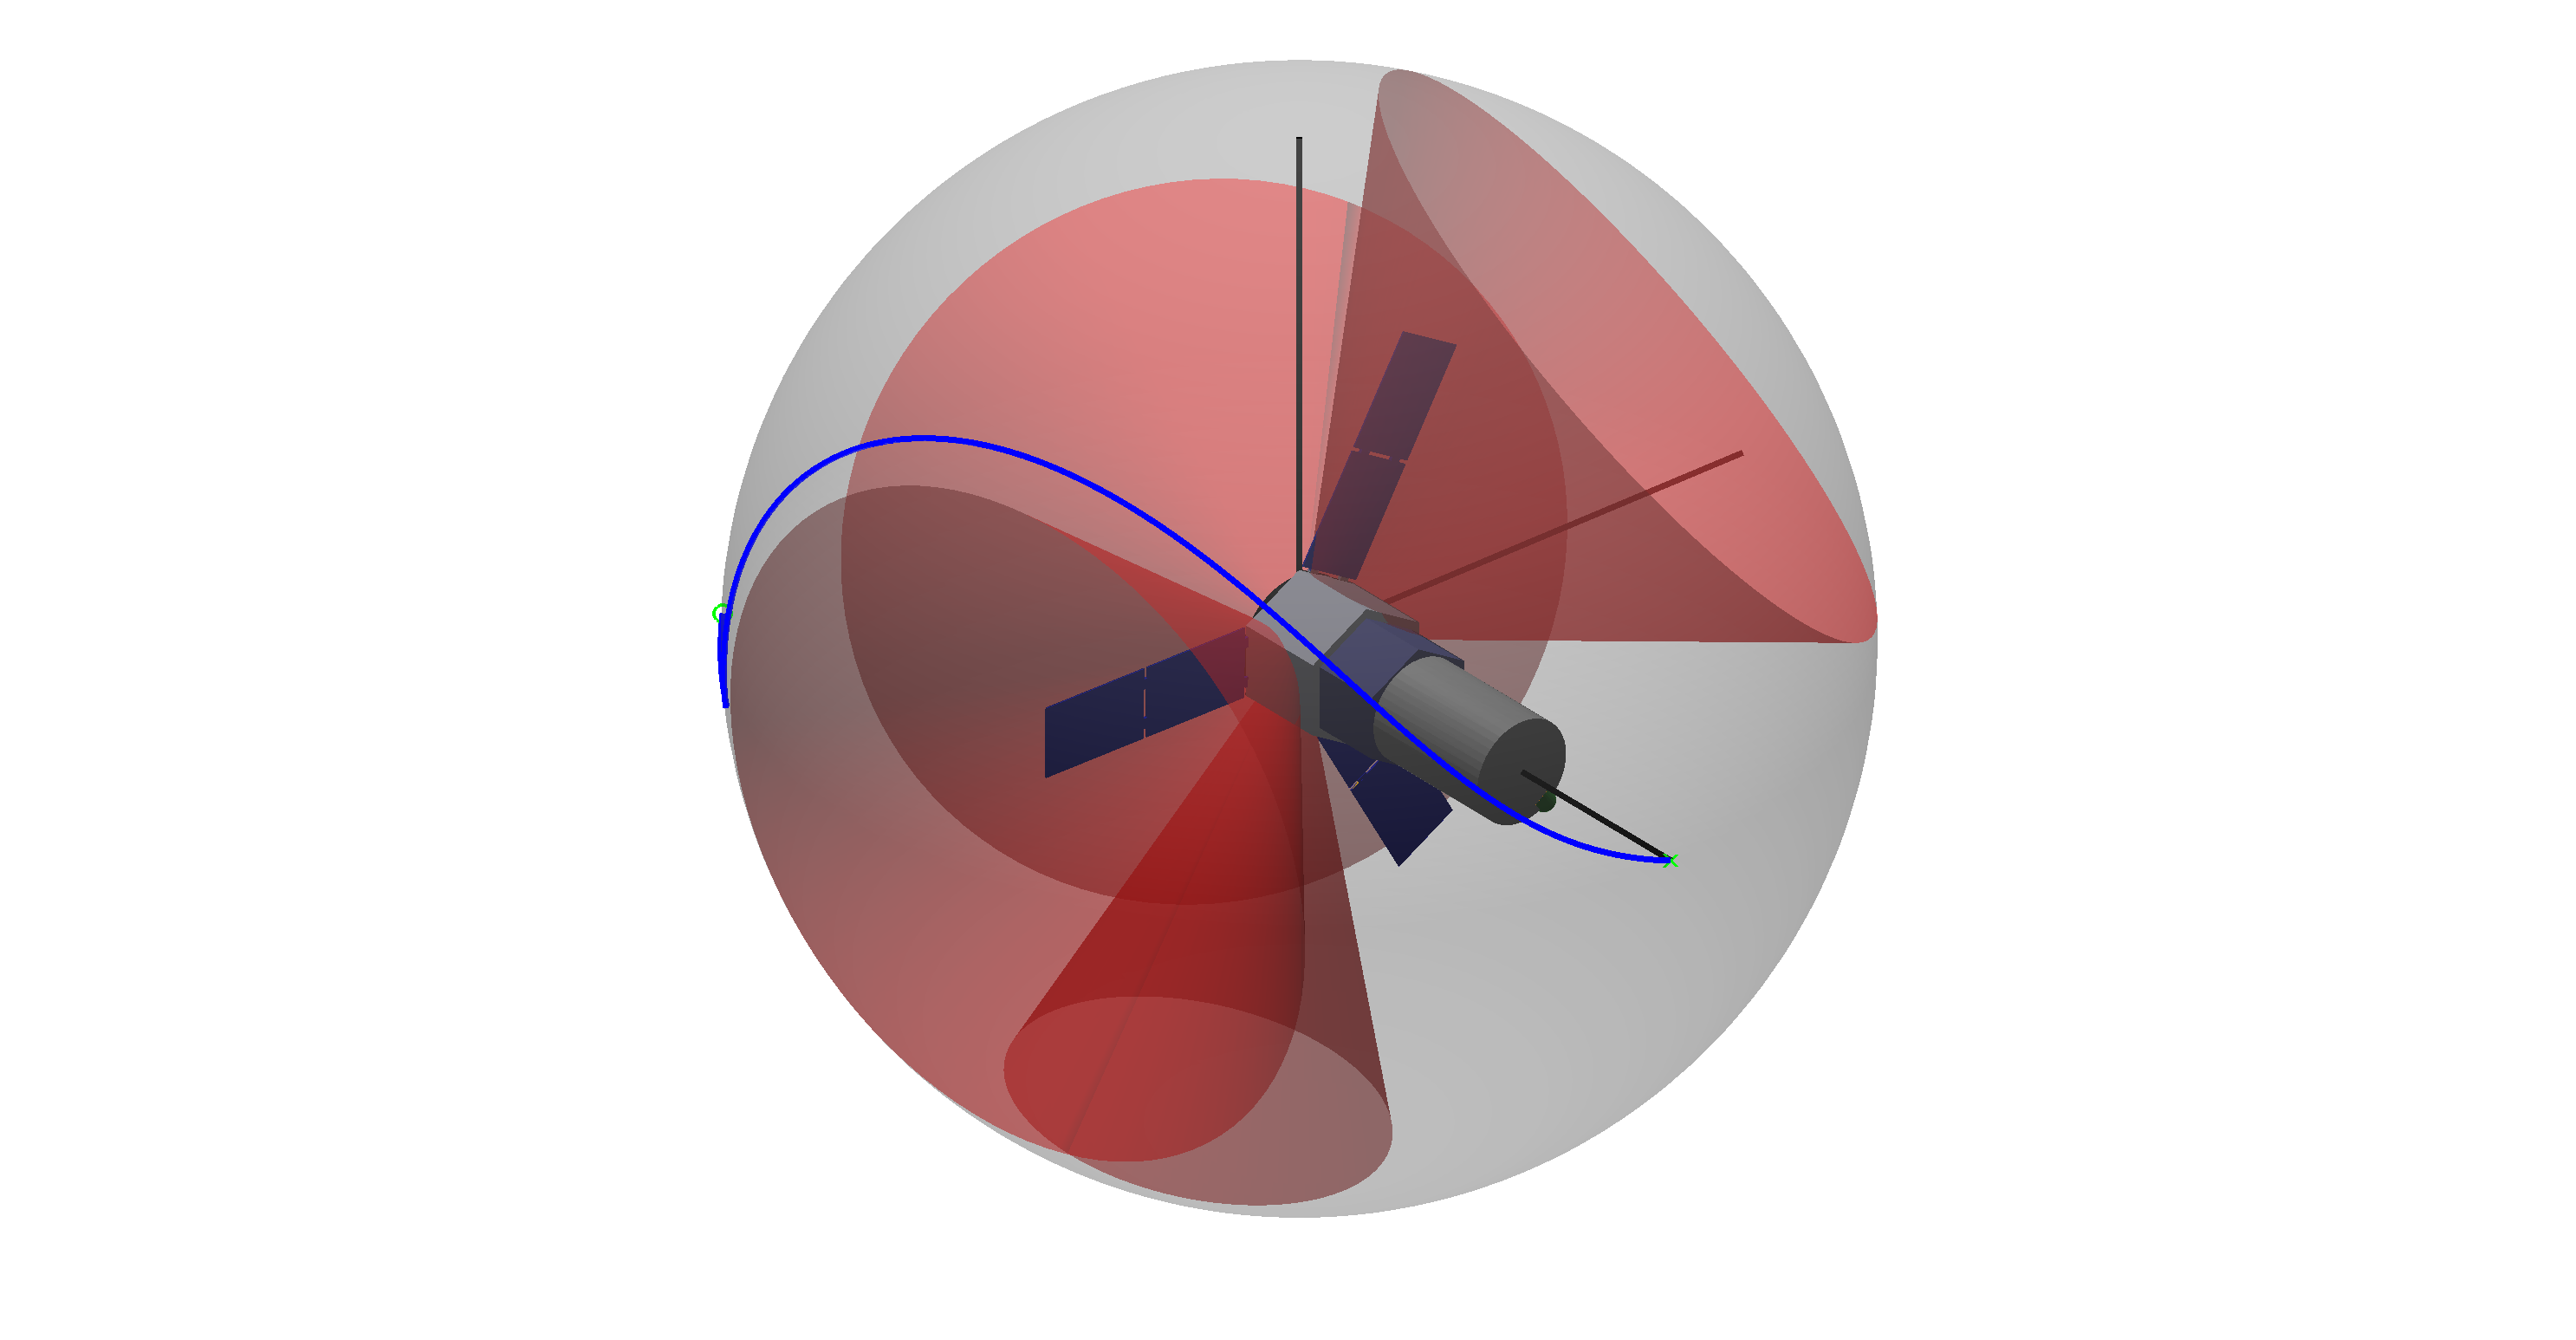
\includegraphics[trim={10cm 0 10cm 0},clip,width=0.4\columnwidth]{cad_adapt} }
  \caption{Attitude stabilization with adaptive update law}
  \label{fig:adapt} 
\end{figure}
\begin{multicols}{2}
\subsection{Attitude Parameterizations}\label{ssec:attitude_parameterization}
% Discuss the benefits of using this geometric representation as compared to Euler angles or quaternions
Attitude parameterizations, such as Euler angles and Quaternions, are frequently used in the aerospace and astrodynamics communities~\cite{vallado2007}.
For example, Euler angle sequences are frequently used to describe the transformation between a variety of reference frames used to describe the position and orientation of the orbit of Earth satellites~\cite{vallado2007}.
In addition, quaternions were used during the operation of Skylab and the NASA Space Shuttle~\cite{hughes2004}.
However, the choice of attitude parameterization plays a critical role in control design and the resulting motion of the system.

% singularities and the problems involved with using Euler angles
Euler angle sequences are a minimum, three-parameter set of angles which describe the transformation between two reference frames.
Using Euler angles, we can represent any general rotation as a sequence of three intermediate rotations~\cite{shuster1993}.
By convention, there are \num{24} possible Euler angle sequences for any given rotation.
In addition, Euler angles are a minimum representation, as only three angles, and the associated sequence, are required to describe the three angular degrees of freedom of the rigid body.
However, there is great ambiguity in the representation of the attitude as there are many equivalent Euler angle sequences for a given attitude of the system.
Therefore, great care must be taken in the control system design to ensure that a consistent sequence is used. 
Furthermore, it has been shown that no minimal attitude representation can describe orientations both globally and without singularities~\cite{hughes2004,bhat2000}.
These singularities can cause significant difficulties during control design and hardware implementation.

To demonstrate the effect of the kinematic singularities inherent with Euler angles we will represent the attitude of the body fixed reference frame, \( \vecbf{b}_i \), with respect to the inertial frame, \( \vecbf{e}_i\), in terms of the 3-1-3 Euler angle sequence.
More explicitly, this corresponds to the rotation sequence \( \theta_1 \vecbf{b}_3 , \theta_2 \vecbf{b}_1, \theta_3 \vecbf{b}_3 \).
The rotation matrix, \( R(\theta_1, \theta_2, \theta_3) \), corresponding to this sequence is 
\begin{align}\label{eq:euler313}
    \begin{bmatrix}
        -s_1 c_2 s_3 + c_3 c_1 & -s_1 c_2 c_3 - s_3 c_1 & s_1s_2 \\
        c_1 c_2 s_3 + c_3 s_1 & c_1 c_2 c_3 - s_3 s_1 & - c_1 s_2 \\
        s_2 s_3 & s_2 c_3 & c_2
    \end{bmatrix} ,
\end{align}
where \( s_i, c_i \) represent \( \sin \theta_i, \cos \theta_i \) for \( i = \braces{1,2,3}\).
Using this representation, the kinematic differential equations for the associated Euler angles are given as
\begin{align}\label{eq:euler313_diff}
    \begin{bmatrix}
        \dot{\theta}_1 \\ \dot{\theta}_2 \\ \dot{\theta}_3 
    \end{bmatrix}
    =
    \begin{bmatrix}
        \slfrac{\parenth{\Omega_1 s_3 + \Omega_2 c_3}}{s_2} \\
        \Omega_1 c_3 - \Omega_2 s_3 \\
        -\slfrac{\parenth{\Omega_1 s_3 + \omega_2 c_3}c_2}{s_2} + \Omega_3
    \end{bmatrix} .
\end{align}
From~\cref{eq:euler313_diff}, it is immediately clear that a singularity exists when \( \sin \theta_2 = 0 \) or equivalently, \( \theta_2 = 0, \pm \pi \). 
In the vicinity of the singularity, the angular velocities of the Euler angles will tend to approach \( \pm \infty \) and the angular velocities will experience instantaneous sign changes.
Furthermore, all Euler angle sequences will exhibit a similar singularity at either \( \theta_2 = 0, \pm \pi \) or \( \theta_2 = \pm \frac{\pi}{2}, \pm \frac{3\pi}{2} \).
Therefore simply switching the sequence does not alleviate the issue, but rather only moves the singularity.
As a result, Euler angles are not appropriate for systems which experience large angular rotations, such as those demonstrated in~\cref{fig:adapt}, or control systems which rely on the angular velocities \( \theta_i \).
% discuss the unwinding phenomenon with quaternions
\subsection{Time-varying Disturbance}\label{ssec:time_varying}
The form of the uncertainty, given in~\cref{eqn:Wdot}, is commonly used in the adaptive control literature~\cite{LeeITCST13,ioannou2012}. 
A wide variety of realistic disturbances, such as gravitational gradients or malfunctioning thrusters for spacecraft scenarios, are accurately represented via this model. 
In addition, it is possible to represent the uncertainty of a time-varying inertia matrix as an equivalent external disturbance. 
For example, Euler's law gives the relationship for the rate of change of angular momentum as
\begin{align*}
    M_{ext} = \dot{\vecbf{H}} = \dot{J} \vecbf{\Omega} + J \dot{\vecbf{\Omega}} .
\end{align*}
Using this, we can see that an instantaneous change in \( J \) is proportional to an external moment.
Finally, it has been shown that this adaptive control formulation is able to handle time-varying disturbances under some mild assumptions~\cite{ioannou2012}. 

We demonstrate the ability to handle an uncertain time-varying disturbance via numerical example.
The system is identical to the one presented in~\Cref{sec:numerical_simulation}, however we modify the external disturbance. 
The external disturbance is the superposition of constant and time-varying terms as
\begin{align*}
    \Delta = \begin{bmatrix} 0.2 \\ 0.2 \\0.2 \end{bmatrix} + 0.02 \begin{bmatrix} \sin 9 t \\ \cos 9 t \\ \frac{1}{2} \parenth{\sin 9t + \cos 9t}\end{bmatrix} \si{\newton\meter}.
\end{align*}
We define a constraint in the inertial frame as \( v = [\frac{1}{\sqrt{2}}, \frac{1}{\sqrt{2}}, 0]^T \) with \( \theta = \ang{12} \).
The initial state is defined as \(R(0) = \exp( \frac{\pi}{2} \hat{e}_3) \), while the desired state is \(R_d =I \).
The goal is to rotate the vehicle about the \( e_3 \) axis while avoiding the obstacle and compensating for the time-varying disturbance. 

\Cref{fig:tv} demonstrates the ability for the adaptive controller, which is presented in~\Cref{prop:adaptive_control}, to handle time-varying disturbances.
\Cref{fig:Psi_tv} shows the non-dimensional value of the configuration error function and demonstrates that the adaptive controller is able to stabilize the system to the desired attitude configuration.
In addition,~\cref{fig:con_angle_tv} shows that the constraint is never violated as the angle between the body-fixed sensor \( r \) and the constraint \( v \) is greater than \SI{12}{\degree} over the entire attitude maneuver.
We can see in~\cref{fig:Delta_tv} that that estimate \(\bar \Delta \) for each of the components accurately tracks the true disturbance after approximately~\SI{5}{\second}.

\section{Experiment on Hexrotor UAV}\label{sec:experiment}
\vspace{-5mm}
\begin{figure}[H]
    \centering
    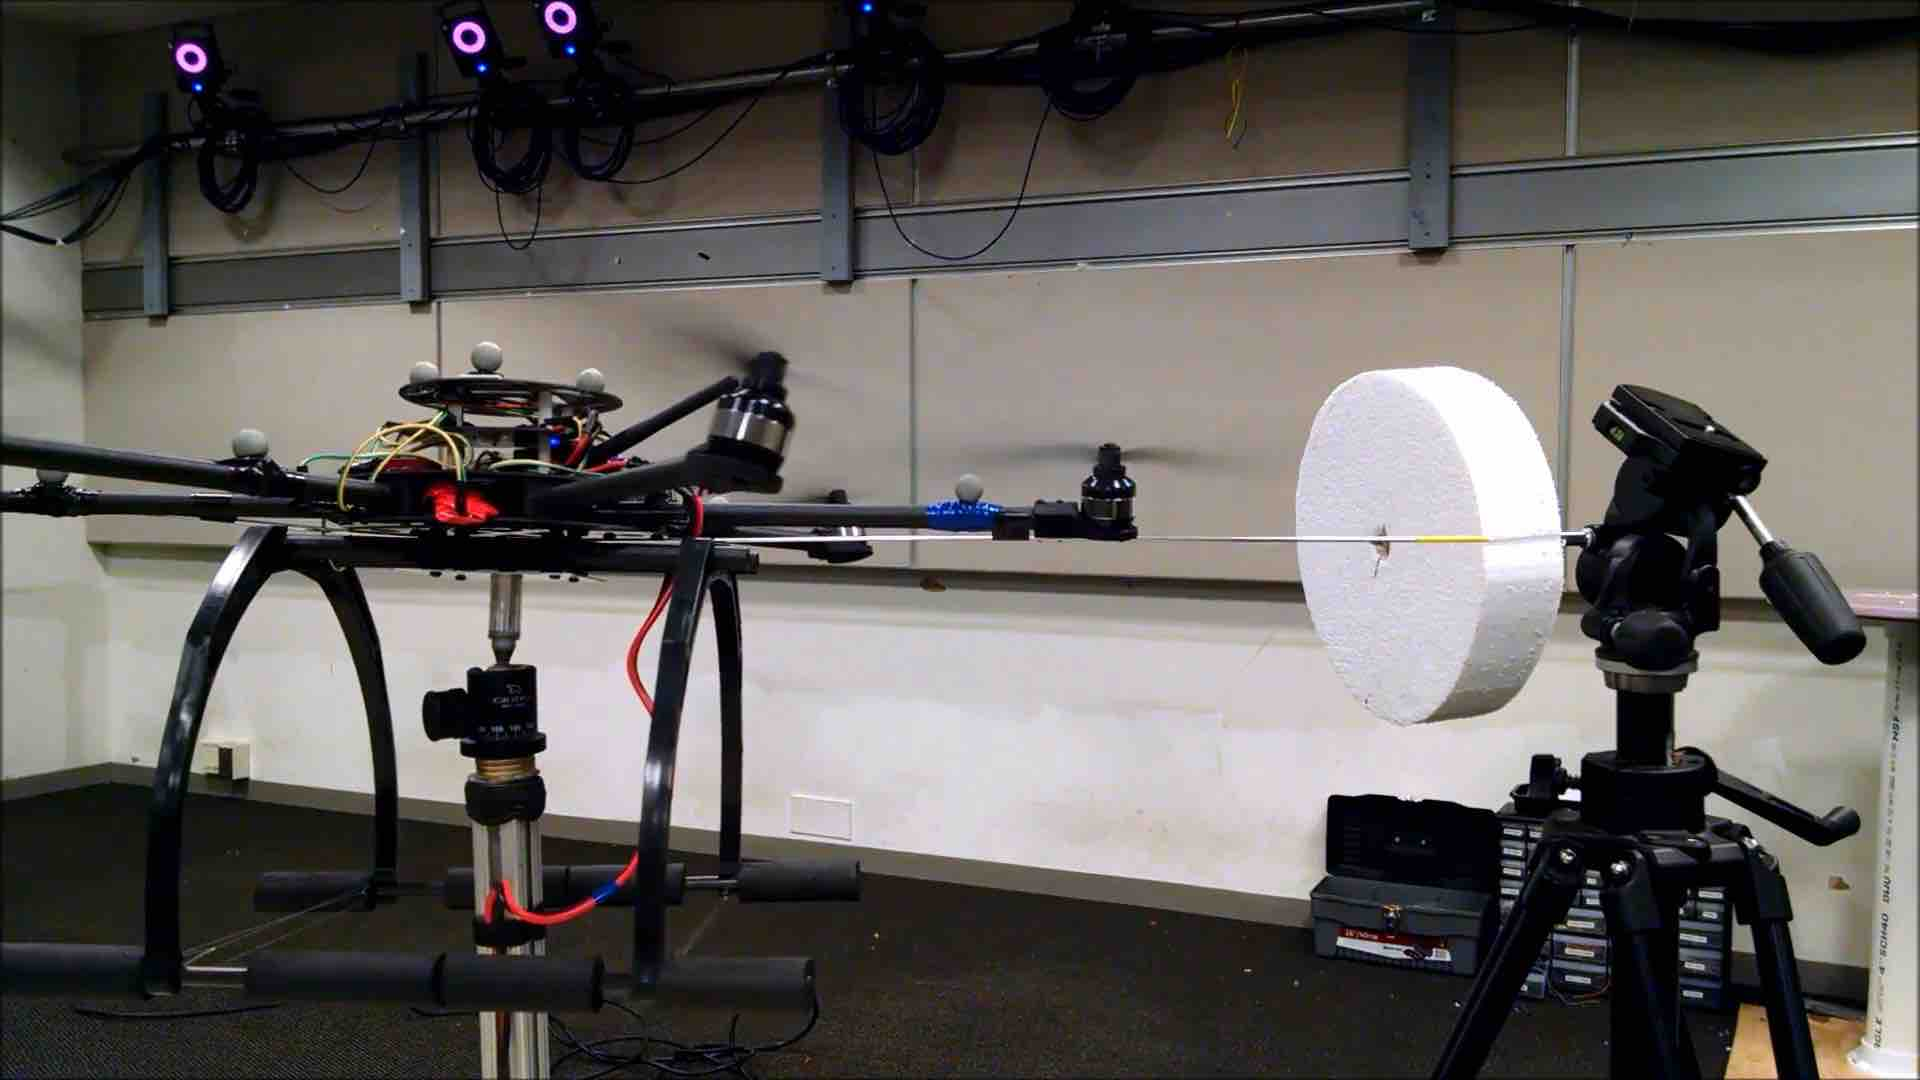
\includegraphics[width = 0.50\columnwidth]{hexrotor}
    \caption{Attitude control testbed~\label{fig:hexrotor}}
\end{figure}
\vspace{-3mm}
A hexrotor unmanned aerial vehicle (UAV), as seen in~\cref{fig:hexrotor}, has been developed at the Flight Dynamics and Controls Laboratory (FDCL) at the George Washington University~\cite{kaufman2014}.
The UAV is composed of three pairs of counter-rotating propellers. 
Typical UAVs are composed of four or more co-planar propellers.
As a result, these systems are underactuated and unable to impart a force along every degree of freedom.
For example, quadrotor UAVs are unable to translate laterally without first conducting a rotation.
Conversely, the propeller pairs of the hexrotor are angled relative to one another to allow for a fully actuated rigid body.
This allows the hexrotor to impart a force in any direction and a moment about any axis. 
\end{multicols}
\begin{figure}[H]
    \centering 
    \subfigure[{Configuration error \( \Psi \)} \label{fig:Psi_tv} ]{%% Creator: Matplotlib, PGF backend
%%
%% To include the figure in your LaTeX document, write
%%   \input{<filename>.pgf}
%%
%% Make sure the required packages are loaded in your preamble
%%   \usepackage{pgf}
%%
%% Figures using additional raster images can only be included by \input if
%% they are in the same directory as the main LaTeX file. For loading figures
%% from other directories you can use the `import` package
%%   \usepackage{import}
%% and then include the figures with
%%   \import{<path to file>}{<filename>.pgf}
%%
%% Matplotlib used the following preamble
%%   \usepackage[utf8x]{inputenc}
%%   \usepackage[T1]{fontenc}
%%   \usepackage{siunitx}
%%
\begingroup%
\makeatletter%
\begin{pgfpicture}%
\pgfpathrectangle{\pgfpointorigin}{\pgfqpoint{2.227534in}{1.887367in}}%
\pgfusepath{use as bounding box, clip}%
\begin{pgfscope}%
\pgfsetbuttcap%
\pgfsetmiterjoin%
\definecolor{currentfill}{rgb}{1.000000,1.000000,1.000000}%
\pgfsetfillcolor{currentfill}%
\pgfsetlinewidth{0.000000pt}%
\definecolor{currentstroke}{rgb}{1.000000,1.000000,1.000000}%
\pgfsetstrokecolor{currentstroke}%
\pgfsetdash{}{0pt}%
\pgfpathmoveto{\pgfqpoint{0.000000in}{0.000000in}}%
\pgfpathlineto{\pgfqpoint{2.227534in}{0.000000in}}%
\pgfpathlineto{\pgfqpoint{2.227534in}{1.887367in}}%
\pgfpathlineto{\pgfqpoint{0.000000in}{1.887367in}}%
\pgfpathclose%
\pgfusepath{fill}%
\end{pgfscope}%
\begin{pgfscope}%
\pgfsetbuttcap%
\pgfsetmiterjoin%
\definecolor{currentfill}{rgb}{1.000000,1.000000,1.000000}%
\pgfsetfillcolor{currentfill}%
\pgfsetlinewidth{0.000000pt}%
\definecolor{currentstroke}{rgb}{0.000000,0.000000,0.000000}%
\pgfsetstrokecolor{currentstroke}%
\pgfsetstrokeopacity{0.000000}%
\pgfsetdash{}{0pt}%
\pgfpathmoveto{\pgfqpoint{0.580782in}{0.481986in}}%
\pgfpathlineto{\pgfqpoint{2.107534in}{0.481986in}}%
\pgfpathlineto{\pgfqpoint{2.107534in}{1.767367in}}%
\pgfpathlineto{\pgfqpoint{0.580782in}{1.767367in}}%
\pgfpathclose%
\pgfusepath{fill}%
\end{pgfscope}%
\begin{pgfscope}%
\pgfpathrectangle{\pgfqpoint{0.580782in}{0.481986in}}{\pgfqpoint{1.526753in}{1.285381in}} %
\pgfusepath{clip}%
\pgfsetroundcap%
\pgfsetroundjoin%
\pgfsetlinewidth{1.003750pt}%
\definecolor{currentstroke}{rgb}{0.800000,0.800000,0.800000}%
\pgfsetstrokecolor{currentstroke}%
\pgfsetdash{}{0pt}%
\pgfpathmoveto{\pgfqpoint{0.650180in}{0.481986in}}%
\pgfpathlineto{\pgfqpoint{0.650180in}{1.767367in}}%
\pgfusepath{stroke}%
\end{pgfscope}%
\begin{pgfscope}%
\definecolor{textcolor}{rgb}{0.150000,0.150000,0.150000}%
\pgfsetstrokecolor{textcolor}%
\pgfsetfillcolor{textcolor}%
\pgftext[x=0.650180in,y=0.384764in,,top]{\color{textcolor}\rmfamily\fontsize{8.000000}{9.600000}\selectfont \(\displaystyle 0\)}%
\end{pgfscope}%
\begin{pgfscope}%
\pgfpathrectangle{\pgfqpoint{0.580782in}{0.481986in}}{\pgfqpoint{1.526753in}{1.285381in}} %
\pgfusepath{clip}%
\pgfsetroundcap%
\pgfsetroundjoin%
\pgfsetlinewidth{1.003750pt}%
\definecolor{currentstroke}{rgb}{0.800000,0.800000,0.800000}%
\pgfsetstrokecolor{currentstroke}%
\pgfsetdash{}{0pt}%
\pgfpathmoveto{\pgfqpoint{1.344158in}{0.481986in}}%
\pgfpathlineto{\pgfqpoint{1.344158in}{1.767367in}}%
\pgfusepath{stroke}%
\end{pgfscope}%
\begin{pgfscope}%
\definecolor{textcolor}{rgb}{0.150000,0.150000,0.150000}%
\pgfsetstrokecolor{textcolor}%
\pgfsetfillcolor{textcolor}%
\pgftext[x=1.344158in,y=0.384764in,,top]{\color{textcolor}\rmfamily\fontsize{8.000000}{9.600000}\selectfont \(\displaystyle 5\)}%
\end{pgfscope}%
\begin{pgfscope}%
\pgfpathrectangle{\pgfqpoint{0.580782in}{0.481986in}}{\pgfqpoint{1.526753in}{1.285381in}} %
\pgfusepath{clip}%
\pgfsetroundcap%
\pgfsetroundjoin%
\pgfsetlinewidth{1.003750pt}%
\definecolor{currentstroke}{rgb}{0.800000,0.800000,0.800000}%
\pgfsetstrokecolor{currentstroke}%
\pgfsetdash{}{0pt}%
\pgfpathmoveto{\pgfqpoint{2.038136in}{0.481986in}}%
\pgfpathlineto{\pgfqpoint{2.038136in}{1.767367in}}%
\pgfusepath{stroke}%
\end{pgfscope}%
\begin{pgfscope}%
\definecolor{textcolor}{rgb}{0.150000,0.150000,0.150000}%
\pgfsetstrokecolor{textcolor}%
\pgfsetfillcolor{textcolor}%
\pgftext[x=2.038136in,y=0.384764in,,top]{\color{textcolor}\rmfamily\fontsize{8.000000}{9.600000}\selectfont \(\displaystyle 10\)}%
\end{pgfscope}%
\begin{pgfscope}%
\definecolor{textcolor}{rgb}{0.150000,0.150000,0.150000}%
\pgfsetstrokecolor{textcolor}%
\pgfsetfillcolor{textcolor}%
\pgftext[x=1.344158in,y=0.231084in,,top]{\color{textcolor}\rmfamily\fontsize{8.000000}{9.600000}\selectfont \(\displaystyle t\) (sec)}%
\end{pgfscope}%
\begin{pgfscope}%
\pgfpathrectangle{\pgfqpoint{0.580782in}{0.481986in}}{\pgfqpoint{1.526753in}{1.285381in}} %
\pgfusepath{clip}%
\pgfsetroundcap%
\pgfsetroundjoin%
\pgfsetlinewidth{1.003750pt}%
\definecolor{currentstroke}{rgb}{0.800000,0.800000,0.800000}%
\pgfsetstrokecolor{currentstroke}%
\pgfsetdash{}{0pt}%
\pgfpathmoveto{\pgfqpoint{0.580782in}{0.540413in}}%
\pgfpathlineto{\pgfqpoint{2.107534in}{0.540413in}}%
\pgfusepath{stroke}%
\end{pgfscope}%
\begin{pgfscope}%
\definecolor{textcolor}{rgb}{0.150000,0.150000,0.150000}%
\pgfsetstrokecolor{textcolor}%
\pgfsetfillcolor{textcolor}%
\pgftext[x=0.273680in,y=0.502150in,left,base]{\color{textcolor}\rmfamily\fontsize{8.000000}{9.600000}\selectfont \(\displaystyle 0.00\)}%
\end{pgfscope}%
\begin{pgfscope}%
\pgfpathrectangle{\pgfqpoint{0.580782in}{0.481986in}}{\pgfqpoint{1.526753in}{1.285381in}} %
\pgfusepath{clip}%
\pgfsetroundcap%
\pgfsetroundjoin%
\pgfsetlinewidth{1.003750pt}%
\definecolor{currentstroke}{rgb}{0.800000,0.800000,0.800000}%
\pgfsetstrokecolor{currentstroke}%
\pgfsetdash{}{0pt}%
\pgfpathmoveto{\pgfqpoint{0.580782in}{0.811940in}}%
\pgfpathlineto{\pgfqpoint{2.107534in}{0.811940in}}%
\pgfusepath{stroke}%
\end{pgfscope}%
\begin{pgfscope}%
\definecolor{textcolor}{rgb}{0.150000,0.150000,0.150000}%
\pgfsetstrokecolor{textcolor}%
\pgfsetfillcolor{textcolor}%
\pgftext[x=0.273680in,y=0.773678in,left,base]{\color{textcolor}\rmfamily\fontsize{8.000000}{9.600000}\selectfont \(\displaystyle 0.25\)}%
\end{pgfscope}%
\begin{pgfscope}%
\pgfpathrectangle{\pgfqpoint{0.580782in}{0.481986in}}{\pgfqpoint{1.526753in}{1.285381in}} %
\pgfusepath{clip}%
\pgfsetroundcap%
\pgfsetroundjoin%
\pgfsetlinewidth{1.003750pt}%
\definecolor{currentstroke}{rgb}{0.800000,0.800000,0.800000}%
\pgfsetstrokecolor{currentstroke}%
\pgfsetdash{}{0pt}%
\pgfpathmoveto{\pgfqpoint{0.580782in}{1.083467in}}%
\pgfpathlineto{\pgfqpoint{2.107534in}{1.083467in}}%
\pgfusepath{stroke}%
\end{pgfscope}%
\begin{pgfscope}%
\definecolor{textcolor}{rgb}{0.150000,0.150000,0.150000}%
\pgfsetstrokecolor{textcolor}%
\pgfsetfillcolor{textcolor}%
\pgftext[x=0.273680in,y=1.045205in,left,base]{\color{textcolor}\rmfamily\fontsize{8.000000}{9.600000}\selectfont \(\displaystyle 0.50\)}%
\end{pgfscope}%
\begin{pgfscope}%
\pgfpathrectangle{\pgfqpoint{0.580782in}{0.481986in}}{\pgfqpoint{1.526753in}{1.285381in}} %
\pgfusepath{clip}%
\pgfsetroundcap%
\pgfsetroundjoin%
\pgfsetlinewidth{1.003750pt}%
\definecolor{currentstroke}{rgb}{0.800000,0.800000,0.800000}%
\pgfsetstrokecolor{currentstroke}%
\pgfsetdash{}{0pt}%
\pgfpathmoveto{\pgfqpoint{0.580782in}{1.354994in}}%
\pgfpathlineto{\pgfqpoint{2.107534in}{1.354994in}}%
\pgfusepath{stroke}%
\end{pgfscope}%
\begin{pgfscope}%
\definecolor{textcolor}{rgb}{0.150000,0.150000,0.150000}%
\pgfsetstrokecolor{textcolor}%
\pgfsetfillcolor{textcolor}%
\pgftext[x=0.273680in,y=1.316732in,left,base]{\color{textcolor}\rmfamily\fontsize{8.000000}{9.600000}\selectfont \(\displaystyle 0.75\)}%
\end{pgfscope}%
\begin{pgfscope}%
\pgfpathrectangle{\pgfqpoint{0.580782in}{0.481986in}}{\pgfqpoint{1.526753in}{1.285381in}} %
\pgfusepath{clip}%
\pgfsetroundcap%
\pgfsetroundjoin%
\pgfsetlinewidth{1.003750pt}%
\definecolor{currentstroke}{rgb}{0.800000,0.800000,0.800000}%
\pgfsetstrokecolor{currentstroke}%
\pgfsetdash{}{0pt}%
\pgfpathmoveto{\pgfqpoint{0.580782in}{1.626522in}}%
\pgfpathlineto{\pgfqpoint{2.107534in}{1.626522in}}%
\pgfusepath{stroke}%
\end{pgfscope}%
\begin{pgfscope}%
\definecolor{textcolor}{rgb}{0.150000,0.150000,0.150000}%
\pgfsetstrokecolor{textcolor}%
\pgfsetfillcolor{textcolor}%
\pgftext[x=0.273680in,y=1.588259in,left,base]{\color{textcolor}\rmfamily\fontsize{8.000000}{9.600000}\selectfont \(\displaystyle 1.00\)}%
\end{pgfscope}%
\begin{pgfscope}%
\definecolor{textcolor}{rgb}{0.150000,0.150000,0.150000}%
\pgfsetstrokecolor{textcolor}%
\pgfsetfillcolor{textcolor}%
\pgftext[x=0.218124in,y=1.124676in,,bottom,rotate=90.000000]{\color{textcolor}\rmfamily\fontsize{8.000000}{9.600000}\selectfont \(\displaystyle \Psi\)}%
\end{pgfscope}%
\begin{pgfscope}%
\pgfpathrectangle{\pgfqpoint{0.580782in}{0.481986in}}{\pgfqpoint{1.526753in}{1.285381in}} %
\pgfusepath{clip}%
\pgfsetroundcap%
\pgfsetroundjoin%
\pgfsetlinewidth{1.003750pt}%
\definecolor{currentstroke}{rgb}{0.298039,0.447059,0.690196}%
\pgfsetstrokecolor{currentstroke}%
\pgfsetdash{}{0pt}%
\pgfpathmoveto{\pgfqpoint{0.650180in}{1.708940in}}%
\pgfpathlineto{\pgfqpoint{0.651569in}{1.706462in}}%
\pgfpathlineto{\pgfqpoint{0.654348in}{1.690129in}}%
\pgfpathlineto{\pgfqpoint{0.659905in}{1.633288in}}%
\pgfpathlineto{\pgfqpoint{0.686303in}{1.329333in}}%
\pgfpathlineto{\pgfqpoint{0.694639in}{1.262563in}}%
\pgfpathlineto{\pgfqpoint{0.700196in}{1.232915in}}%
\pgfpathlineto{\pgfqpoint{0.714089in}{1.179262in}}%
\pgfpathlineto{\pgfqpoint{0.722426in}{1.131458in}}%
\pgfpathlineto{\pgfqpoint{0.732151in}{1.058531in}}%
\pgfpathlineto{\pgfqpoint{0.758549in}{0.847658in}}%
\pgfpathlineto{\pgfqpoint{0.768274in}{0.790528in}}%
\pgfpathlineto{\pgfqpoint{0.777999in}{0.745792in}}%
\pgfpathlineto{\pgfqpoint{0.787725in}{0.710723in}}%
\pgfpathlineto{\pgfqpoint{0.798840in}{0.679303in}}%
\pgfpathlineto{\pgfqpoint{0.809954in}{0.654616in}}%
\pgfpathlineto{\pgfqpoint{0.821069in}{0.635011in}}%
\pgfpathlineto{\pgfqpoint{0.832184in}{0.619443in}}%
\pgfpathlineto{\pgfqpoint{0.844688in}{0.605799in}}%
\pgfpathlineto{\pgfqpoint{0.857192in}{0.595314in}}%
\pgfpathlineto{\pgfqpoint{0.872475in}{0.585412in}}%
\pgfpathlineto{\pgfqpoint{0.893315in}{0.574772in}}%
\pgfpathlineto{\pgfqpoint{0.915545in}{0.565837in}}%
\pgfpathlineto{\pgfqpoint{0.936385in}{0.559876in}}%
\pgfpathlineto{\pgfqpoint{0.961393in}{0.555273in}}%
\pgfpathlineto{\pgfqpoint{1.018356in}{0.547860in}}%
\pgfpathlineto{\pgfqpoint{1.054479in}{0.545509in}}%
\pgfpathlineto{\pgfqpoint{1.162848in}{0.542040in}}%
\pgfpathlineto{\pgfqpoint{1.383754in}{0.540594in}}%
\pgfpathlineto{\pgfqpoint{1.719976in}{0.540455in}}%
\pgfpathlineto{\pgfqpoint{2.038136in}{0.540465in}}%
\pgfpathlineto{\pgfqpoint{2.038136in}{0.540465in}}%
\pgfusepath{stroke}%
\end{pgfscope}%
\begin{pgfscope}%
\pgfpathrectangle{\pgfqpoint{0.580782in}{0.481986in}}{\pgfqpoint{1.526753in}{1.285381in}} %
\pgfusepath{clip}%
\pgfsetbuttcap%
\pgfsetroundjoin%
\pgfsetlinewidth{1.003750pt}%
\definecolor{currentstroke}{rgb}{0.333333,0.658824,0.407843}%
\pgfsetstrokecolor{currentstroke}%
\pgfsetdash{{5.600000pt}{2.400000pt}}{0.000000pt}%
\pgfpathmoveto{\pgfqpoint{0.650180in}{0.540413in}}%
\pgfpathlineto{\pgfqpoint{2.038136in}{0.540413in}}%
\pgfpathlineto{\pgfqpoint{2.038136in}{0.540413in}}%
\pgfusepath{stroke}%
\end{pgfscope}%
\begin{pgfscope}%
\pgfsetrectcap%
\pgfsetmiterjoin%
\pgfsetlinewidth{1.003750pt}%
\definecolor{currentstroke}{rgb}{0.800000,0.800000,0.800000}%
\pgfsetstrokecolor{currentstroke}%
\pgfsetdash{}{0pt}%
\pgfpathmoveto{\pgfqpoint{0.580782in}{0.481986in}}%
\pgfpathlineto{\pgfqpoint{0.580782in}{1.767367in}}%
\pgfusepath{stroke}%
\end{pgfscope}%
\begin{pgfscope}%
\pgfsetrectcap%
\pgfsetmiterjoin%
\pgfsetlinewidth{1.003750pt}%
\definecolor{currentstroke}{rgb}{0.800000,0.800000,0.800000}%
\pgfsetstrokecolor{currentstroke}%
\pgfsetdash{}{0pt}%
\pgfpathmoveto{\pgfqpoint{2.107534in}{0.481986in}}%
\pgfpathlineto{\pgfqpoint{2.107534in}{1.767367in}}%
\pgfusepath{stroke}%
\end{pgfscope}%
\begin{pgfscope}%
\pgfsetrectcap%
\pgfsetmiterjoin%
\pgfsetlinewidth{1.003750pt}%
\definecolor{currentstroke}{rgb}{0.800000,0.800000,0.800000}%
\pgfsetstrokecolor{currentstroke}%
\pgfsetdash{}{0pt}%
\pgfpathmoveto{\pgfqpoint{0.580782in}{0.481986in}}%
\pgfpathlineto{\pgfqpoint{2.107534in}{0.481986in}}%
\pgfusepath{stroke}%
\end{pgfscope}%
\begin{pgfscope}%
\pgfsetrectcap%
\pgfsetmiterjoin%
\pgfsetlinewidth{1.003750pt}%
\definecolor{currentstroke}{rgb}{0.800000,0.800000,0.800000}%
\pgfsetstrokecolor{currentstroke}%
\pgfsetdash{}{0pt}%
\pgfpathmoveto{\pgfqpoint{0.580782in}{1.767367in}}%
\pgfpathlineto{\pgfqpoint{2.107534in}{1.767367in}}%
\pgfusepath{stroke}%
\end{pgfscope}%
\end{pgfpicture}%
\makeatother%
\endgroup%
}~
    \subfigure[{Angle to constraint } \label{fig:con_angle_tv}]{%% Creator: Matplotlib, PGF backend
%%
%% To include the figure in your LaTeX document, write
%%   \input{<filename>.pgf}
%%
%% Make sure the required packages are loaded in your preamble
%%   \usepackage{pgf}
%%
%% Figures using additional raster images can only be included by \input if
%% they are in the same directory as the main LaTeX file. For loading figures
%% from other directories you can use the `import` package
%%   \usepackage{import}
%% and then include the figures with
%%   \import{<path to file>}{<filename>.pgf}
%%
%% Matplotlib used the following preamble
%%   \usepackage[utf8x]{inputenc}
%%   \usepackage[T1]{fontenc}
%%   \usepackage{siunitx}
%%
\begingroup%
\makeatletter%
\begin{pgfpicture}%
\pgfpathrectangle{\pgfpointorigin}{\pgfqpoint{2.227534in}{1.887367in}}%
\pgfusepath{use as bounding box, clip}%
\begin{pgfscope}%
\pgfsetbuttcap%
\pgfsetmiterjoin%
\definecolor{currentfill}{rgb}{1.000000,1.000000,1.000000}%
\pgfsetfillcolor{currentfill}%
\pgfsetlinewidth{0.000000pt}%
\definecolor{currentstroke}{rgb}{1.000000,1.000000,1.000000}%
\pgfsetstrokecolor{currentstroke}%
\pgfsetdash{}{0pt}%
\pgfpathmoveto{\pgfqpoint{0.000000in}{0.000000in}}%
\pgfpathlineto{\pgfqpoint{2.227534in}{0.000000in}}%
\pgfpathlineto{\pgfqpoint{2.227534in}{1.887367in}}%
\pgfpathlineto{\pgfqpoint{0.000000in}{1.887367in}}%
\pgfpathclose%
\pgfusepath{fill}%
\end{pgfscope}%
\begin{pgfscope}%
\pgfsetbuttcap%
\pgfsetmiterjoin%
\definecolor{currentfill}{rgb}{1.000000,1.000000,1.000000}%
\pgfsetfillcolor{currentfill}%
\pgfsetlinewidth{0.000000pt}%
\definecolor{currentstroke}{rgb}{0.000000,0.000000,0.000000}%
\pgfsetstrokecolor{currentstroke}%
\pgfsetstrokeopacity{0.000000}%
\pgfsetdash{}{0pt}%
\pgfpathmoveto{\pgfqpoint{0.521715in}{0.481986in}}%
\pgfpathlineto{\pgfqpoint{2.107534in}{0.481986in}}%
\pgfpathlineto{\pgfqpoint{2.107534in}{1.767367in}}%
\pgfpathlineto{\pgfqpoint{0.521715in}{1.767367in}}%
\pgfpathclose%
\pgfusepath{fill}%
\end{pgfscope}%
\begin{pgfscope}%
\pgfpathrectangle{\pgfqpoint{0.521715in}{0.481986in}}{\pgfqpoint{1.585820in}{1.285381in}} %
\pgfusepath{clip}%
\pgfsetroundcap%
\pgfsetroundjoin%
\pgfsetlinewidth{1.003750pt}%
\definecolor{currentstroke}{rgb}{0.800000,0.800000,0.800000}%
\pgfsetstrokecolor{currentstroke}%
\pgfsetdash{}{0pt}%
\pgfpathmoveto{\pgfqpoint{0.593797in}{0.481986in}}%
\pgfpathlineto{\pgfqpoint{0.593797in}{1.767367in}}%
\pgfusepath{stroke}%
\end{pgfscope}%
\begin{pgfscope}%
\definecolor{textcolor}{rgb}{0.150000,0.150000,0.150000}%
\pgfsetstrokecolor{textcolor}%
\pgfsetfillcolor{textcolor}%
\pgftext[x=0.593797in,y=0.384764in,,top]{\color{textcolor}\rmfamily\fontsize{8.000000}{9.600000}\selectfont \(\displaystyle 0\)}%
\end{pgfscope}%
\begin{pgfscope}%
\pgfpathrectangle{\pgfqpoint{0.521715in}{0.481986in}}{\pgfqpoint{1.585820in}{1.285381in}} %
\pgfusepath{clip}%
\pgfsetroundcap%
\pgfsetroundjoin%
\pgfsetlinewidth{1.003750pt}%
\definecolor{currentstroke}{rgb}{0.800000,0.800000,0.800000}%
\pgfsetstrokecolor{currentstroke}%
\pgfsetdash{}{0pt}%
\pgfpathmoveto{\pgfqpoint{1.314624in}{0.481986in}}%
\pgfpathlineto{\pgfqpoint{1.314624in}{1.767367in}}%
\pgfusepath{stroke}%
\end{pgfscope}%
\begin{pgfscope}%
\definecolor{textcolor}{rgb}{0.150000,0.150000,0.150000}%
\pgfsetstrokecolor{textcolor}%
\pgfsetfillcolor{textcolor}%
\pgftext[x=1.314624in,y=0.384764in,,top]{\color{textcolor}\rmfamily\fontsize{8.000000}{9.600000}\selectfont \(\displaystyle 5\)}%
\end{pgfscope}%
\begin{pgfscope}%
\pgfpathrectangle{\pgfqpoint{0.521715in}{0.481986in}}{\pgfqpoint{1.585820in}{1.285381in}} %
\pgfusepath{clip}%
\pgfsetroundcap%
\pgfsetroundjoin%
\pgfsetlinewidth{1.003750pt}%
\definecolor{currentstroke}{rgb}{0.800000,0.800000,0.800000}%
\pgfsetstrokecolor{currentstroke}%
\pgfsetdash{}{0pt}%
\pgfpathmoveto{\pgfqpoint{2.035452in}{0.481986in}}%
\pgfpathlineto{\pgfqpoint{2.035452in}{1.767367in}}%
\pgfusepath{stroke}%
\end{pgfscope}%
\begin{pgfscope}%
\definecolor{textcolor}{rgb}{0.150000,0.150000,0.150000}%
\pgfsetstrokecolor{textcolor}%
\pgfsetfillcolor{textcolor}%
\pgftext[x=2.035452in,y=0.384764in,,top]{\color{textcolor}\rmfamily\fontsize{8.000000}{9.600000}\selectfont \(\displaystyle 10\)}%
\end{pgfscope}%
\begin{pgfscope}%
\definecolor{textcolor}{rgb}{0.150000,0.150000,0.150000}%
\pgfsetstrokecolor{textcolor}%
\pgfsetfillcolor{textcolor}%
\pgftext[x=1.314624in,y=0.231084in,,top]{\color{textcolor}\rmfamily\fontsize{8.000000}{9.600000}\selectfont \(\displaystyle t\) (sec)}%
\end{pgfscope}%
\begin{pgfscope}%
\pgfpathrectangle{\pgfqpoint{0.521715in}{0.481986in}}{\pgfqpoint{1.585820in}{1.285381in}} %
\pgfusepath{clip}%
\pgfsetroundcap%
\pgfsetroundjoin%
\pgfsetlinewidth{1.003750pt}%
\definecolor{currentstroke}{rgb}{0.800000,0.800000,0.800000}%
\pgfsetstrokecolor{currentstroke}%
\pgfsetdash{}{0pt}%
\pgfpathmoveto{\pgfqpoint{0.521715in}{0.780620in}}%
\pgfpathlineto{\pgfqpoint{2.107534in}{0.780620in}}%
\pgfusepath{stroke}%
\end{pgfscope}%
\begin{pgfscope}%
\definecolor{textcolor}{rgb}{0.150000,0.150000,0.150000}%
\pgfsetstrokecolor{textcolor}%
\pgfsetfillcolor{textcolor}%
\pgftext[x=0.306435in,y=0.742358in,left,base]{\color{textcolor}\rmfamily\fontsize{8.000000}{9.600000}\selectfont \(\displaystyle 20\)}%
\end{pgfscope}%
\begin{pgfscope}%
\pgfpathrectangle{\pgfqpoint{0.521715in}{0.481986in}}{\pgfqpoint{1.585820in}{1.285381in}} %
\pgfusepath{clip}%
\pgfsetroundcap%
\pgfsetroundjoin%
\pgfsetlinewidth{1.003750pt}%
\definecolor{currentstroke}{rgb}{0.800000,0.800000,0.800000}%
\pgfsetstrokecolor{currentstroke}%
\pgfsetdash{}{0pt}%
\pgfpathmoveto{\pgfqpoint{0.521715in}{1.147971in}}%
\pgfpathlineto{\pgfqpoint{2.107534in}{1.147971in}}%
\pgfusepath{stroke}%
\end{pgfscope}%
\begin{pgfscope}%
\definecolor{textcolor}{rgb}{0.150000,0.150000,0.150000}%
\pgfsetstrokecolor{textcolor}%
\pgfsetfillcolor{textcolor}%
\pgftext[x=0.306435in,y=1.109709in,left,base]{\color{textcolor}\rmfamily\fontsize{8.000000}{9.600000}\selectfont \(\displaystyle 30\)}%
\end{pgfscope}%
\begin{pgfscope}%
\pgfpathrectangle{\pgfqpoint{0.521715in}{0.481986in}}{\pgfqpoint{1.585820in}{1.285381in}} %
\pgfusepath{clip}%
\pgfsetroundcap%
\pgfsetroundjoin%
\pgfsetlinewidth{1.003750pt}%
\definecolor{currentstroke}{rgb}{0.800000,0.800000,0.800000}%
\pgfsetstrokecolor{currentstroke}%
\pgfsetdash{}{0pt}%
\pgfpathmoveto{\pgfqpoint{0.521715in}{1.515323in}}%
\pgfpathlineto{\pgfqpoint{2.107534in}{1.515323in}}%
\pgfusepath{stroke}%
\end{pgfscope}%
\begin{pgfscope}%
\definecolor{textcolor}{rgb}{0.150000,0.150000,0.150000}%
\pgfsetstrokecolor{textcolor}%
\pgfsetfillcolor{textcolor}%
\pgftext[x=0.306435in,y=1.477060in,left,base]{\color{textcolor}\rmfamily\fontsize{8.000000}{9.600000}\selectfont \(\displaystyle 40\)}%
\end{pgfscope}%
\begin{pgfscope}%
\definecolor{textcolor}{rgb}{0.150000,0.150000,0.150000}%
\pgfsetstrokecolor{textcolor}%
\pgfsetfillcolor{textcolor}%
\pgftext[x=0.250880in,y=1.124676in,,bottom,rotate=90.000000]{\color{textcolor}\rmfamily\fontsize{8.000000}{9.600000}\selectfont \(\displaystyle \arccos (r^T R^T v_i)\)}%
\end{pgfscope}%
\begin{pgfscope}%
\pgfpathrectangle{\pgfqpoint{0.521715in}{0.481986in}}{\pgfqpoint{1.585820in}{1.285381in}} %
\pgfusepath{clip}%
\pgfsetroundcap%
\pgfsetroundjoin%
\pgfsetlinewidth{1.003750pt}%
\definecolor{currentstroke}{rgb}{0.298039,0.447059,0.690196}%
\pgfsetstrokecolor{currentstroke}%
\pgfsetdash{}{0pt}%
\pgfpathmoveto{\pgfqpoint{0.593797in}{1.698998in}}%
\pgfpathlineto{\pgfqpoint{0.595241in}{1.693721in}}%
\pgfpathlineto{\pgfqpoint{0.598127in}{1.658834in}}%
\pgfpathlineto{\pgfqpoint{0.603899in}{1.536490in}}%
\pgfpathlineto{\pgfqpoint{0.637090in}{0.730731in}}%
\pgfpathlineto{\pgfqpoint{0.644306in}{0.609554in}}%
\pgfpathlineto{\pgfqpoint{0.648635in}{0.560160in}}%
\pgfpathlineto{\pgfqpoint{0.651521in}{0.543156in}}%
\pgfpathlineto{\pgfqpoint{0.652964in}{0.540413in}}%
\pgfpathlineto{\pgfqpoint{0.654408in}{0.541173in}}%
\pgfpathlineto{\pgfqpoint{0.657294in}{0.549661in}}%
\pgfpathlineto{\pgfqpoint{0.665952in}{0.580639in}}%
\pgfpathlineto{\pgfqpoint{0.678940in}{0.618548in}}%
\pgfpathlineto{\pgfqpoint{0.686156in}{0.650341in}}%
\pgfpathlineto{\pgfqpoint{0.694814in}{0.701144in}}%
\pgfpathlineto{\pgfqpoint{0.707802in}{0.794427in}}%
\pgfpathlineto{\pgfqpoint{0.726562in}{0.927682in}}%
\pgfpathlineto{\pgfqpoint{0.738107in}{0.994949in}}%
\pgfpathlineto{\pgfqpoint{0.751095in}{1.057248in}}%
\pgfpathlineto{\pgfqpoint{0.771298in}{1.140732in}}%
\pgfpathlineto{\pgfqpoint{0.814591in}{1.312021in}}%
\pgfpathlineto{\pgfqpoint{0.824693in}{1.341402in}}%
\pgfpathlineto{\pgfqpoint{0.833352in}{1.360571in}}%
\pgfpathlineto{\pgfqpoint{0.842010in}{1.374666in}}%
\pgfpathlineto{\pgfqpoint{0.852112in}{1.386616in}}%
\pgfpathlineto{\pgfqpoint{0.873758in}{1.409967in}}%
\pgfpathlineto{\pgfqpoint{0.883860in}{1.425217in}}%
\pgfpathlineto{\pgfqpoint{0.895405in}{1.447026in}}%
\pgfpathlineto{\pgfqpoint{0.919937in}{1.495340in}}%
\pgfpathlineto{\pgfqpoint{0.928596in}{1.507466in}}%
\pgfpathlineto{\pgfqpoint{0.935811in}{1.514438in}}%
\pgfpathlineto{\pgfqpoint{0.943027in}{1.518746in}}%
\pgfpathlineto{\pgfqpoint{0.951686in}{1.521331in}}%
\pgfpathlineto{\pgfqpoint{0.971889in}{1.525771in}}%
\pgfpathlineto{\pgfqpoint{0.979104in}{1.529833in}}%
\pgfpathlineto{\pgfqpoint{0.987763in}{1.537573in}}%
\pgfpathlineto{\pgfqpoint{0.997865in}{1.550183in}}%
\pgfpathlineto{\pgfqpoint{1.023840in}{1.585255in}}%
\pgfpathlineto{\pgfqpoint{1.032499in}{1.592191in}}%
\pgfpathlineto{\pgfqpoint{1.039714in}{1.595139in}}%
\pgfpathlineto{\pgfqpoint{1.046930in}{1.595813in}}%
\pgfpathlineto{\pgfqpoint{1.057032in}{1.594350in}}%
\pgfpathlineto{\pgfqpoint{1.071463in}{1.592353in}}%
\pgfpathlineto{\pgfqpoint{1.078678in}{1.593436in}}%
\pgfpathlineto{\pgfqpoint{1.085894in}{1.596663in}}%
\pgfpathlineto{\pgfqpoint{1.094552in}{1.603404in}}%
\pgfpathlineto{\pgfqpoint{1.106097in}{1.615833in}}%
\pgfpathlineto{\pgfqpoint{1.121971in}{1.632806in}}%
\pgfpathlineto{\pgfqpoint{1.130630in}{1.638751in}}%
\pgfpathlineto{\pgfqpoint{1.137845in}{1.641044in}}%
\pgfpathlineto{\pgfqpoint{1.145061in}{1.640990in}}%
\pgfpathlineto{\pgfqpoint{1.153719in}{1.638603in}}%
\pgfpathlineto{\pgfqpoint{1.173923in}{1.631806in}}%
\pgfpathlineto{\pgfqpoint{1.181138in}{1.631866in}}%
\pgfpathlineto{\pgfqpoint{1.188353in}{1.634126in}}%
\pgfpathlineto{\pgfqpoint{1.197012in}{1.639666in}}%
\pgfpathlineto{\pgfqpoint{1.210000in}{1.651654in}}%
\pgfpathlineto{\pgfqpoint{1.222988in}{1.663068in}}%
\pgfpathlineto{\pgfqpoint{1.231646in}{1.667663in}}%
\pgfpathlineto{\pgfqpoint{1.238862in}{1.668908in}}%
\pgfpathlineto{\pgfqpoint{1.246077in}{1.667870in}}%
\pgfpathlineto{\pgfqpoint{1.256179in}{1.663649in}}%
\pgfpathlineto{\pgfqpoint{1.273496in}{1.655594in}}%
\pgfpathlineto{\pgfqpoint{1.280712in}{1.654442in}}%
\pgfpathlineto{\pgfqpoint{1.287927in}{1.655452in}}%
\pgfpathlineto{\pgfqpoint{1.295143in}{1.658682in}}%
\pgfpathlineto{\pgfqpoint{1.305244in}{1.666110in}}%
\pgfpathlineto{\pgfqpoint{1.325448in}{1.681998in}}%
\pgfpathlineto{\pgfqpoint{1.332663in}{1.684895in}}%
\pgfpathlineto{\pgfqpoint{1.339879in}{1.685462in}}%
\pgfpathlineto{\pgfqpoint{1.347094in}{1.683790in}}%
\pgfpathlineto{\pgfqpoint{1.357196in}{1.678762in}}%
\pgfpathlineto{\pgfqpoint{1.374513in}{1.669524in}}%
\pgfpathlineto{\pgfqpoint{1.381729in}{1.667931in}}%
\pgfpathlineto{\pgfqpoint{1.388944in}{1.668514in}}%
\pgfpathlineto{\pgfqpoint{1.396159in}{1.671317in}}%
\pgfpathlineto{\pgfqpoint{1.406261in}{1.678133in}}%
\pgfpathlineto{\pgfqpoint{1.426465in}{1.692711in}}%
\pgfpathlineto{\pgfqpoint{1.433680in}{1.695135in}}%
\pgfpathlineto{\pgfqpoint{1.440895in}{1.695247in}}%
\pgfpathlineto{\pgfqpoint{1.448111in}{1.693155in}}%
\pgfpathlineto{\pgfqpoint{1.458213in}{1.687613in}}%
\pgfpathlineto{\pgfqpoint{1.475530in}{1.677707in}}%
\pgfpathlineto{\pgfqpoint{1.482745in}{1.675894in}}%
\pgfpathlineto{\pgfqpoint{1.489961in}{1.676271in}}%
\pgfpathlineto{\pgfqpoint{1.497176in}{1.678865in}}%
\pgfpathlineto{\pgfqpoint{1.507278in}{1.685356in}}%
\pgfpathlineto{\pgfqpoint{1.526038in}{1.698437in}}%
\pgfpathlineto{\pgfqpoint{1.533254in}{1.700968in}}%
\pgfpathlineto{\pgfqpoint{1.540469in}{1.701227in}}%
\pgfpathlineto{\pgfqpoint{1.547685in}{1.699247in}}%
\pgfpathlineto{\pgfqpoint{1.557786in}{1.693688in}}%
\pgfpathlineto{\pgfqpoint{1.576547in}{1.682478in}}%
\pgfpathlineto{\pgfqpoint{1.583762in}{1.680578in}}%
\pgfpathlineto{\pgfqpoint{1.590978in}{1.680881in}}%
\pgfpathlineto{\pgfqpoint{1.598193in}{1.683395in}}%
\pgfpathlineto{\pgfqpoint{1.608295in}{1.689729in}}%
\pgfpathlineto{\pgfqpoint{1.627055in}{1.702321in}}%
\pgfpathlineto{\pgfqpoint{1.634271in}{1.704613in}}%
\pgfpathlineto{\pgfqpoint{1.641486in}{1.704634in}}%
\pgfpathlineto{\pgfqpoint{1.648701in}{1.702435in}}%
\pgfpathlineto{\pgfqpoint{1.658803in}{1.696635in}}%
\pgfpathlineto{\pgfqpoint{1.677563in}{1.685231in}}%
\pgfpathlineto{\pgfqpoint{1.684779in}{1.683323in}}%
\pgfpathlineto{\pgfqpoint{1.691994in}{1.683631in}}%
\pgfpathlineto{\pgfqpoint{1.699210in}{1.686141in}}%
\pgfpathlineto{\pgfqpoint{1.709312in}{1.692417in}}%
\pgfpathlineto{\pgfqpoint{1.728072in}{1.704675in}}%
\pgfpathlineto{\pgfqpoint{1.735287in}{1.706782in}}%
\pgfpathlineto{\pgfqpoint{1.742503in}{1.706612in}}%
\pgfpathlineto{\pgfqpoint{1.749718in}{1.704243in}}%
\pgfpathlineto{\pgfqpoint{1.759820in}{1.698268in}}%
\pgfpathlineto{\pgfqpoint{1.777137in}{1.687407in}}%
\pgfpathlineto{\pgfqpoint{1.785796in}{1.684926in}}%
\pgfpathlineto{\pgfqpoint{1.793011in}{1.685284in}}%
\pgfpathlineto{\pgfqpoint{1.800227in}{1.687834in}}%
\pgfpathlineto{\pgfqpoint{1.810328in}{1.694110in}}%
\pgfpathlineto{\pgfqpoint{1.827646in}{1.705485in}}%
\pgfpathlineto{\pgfqpoint{1.834861in}{1.707862in}}%
\pgfpathlineto{\pgfqpoint{1.842077in}{1.707996in}}%
\pgfpathlineto{\pgfqpoint{1.849292in}{1.705890in}}%
\pgfpathlineto{\pgfqpoint{1.859394in}{1.700110in}}%
\pgfpathlineto{\pgfqpoint{1.879597in}{1.687657in}}%
\pgfpathlineto{\pgfqpoint{1.886813in}{1.685857in}}%
\pgfpathlineto{\pgfqpoint{1.894028in}{1.686293in}}%
\pgfpathlineto{\pgfqpoint{1.901244in}{1.688908in}}%
\pgfpathlineto{\pgfqpoint{1.911345in}{1.695216in}}%
\pgfpathlineto{\pgfqpoint{1.928662in}{1.706423in}}%
\pgfpathlineto{\pgfqpoint{1.935878in}{1.708665in}}%
\pgfpathlineto{\pgfqpoint{1.943093in}{1.708655in}}%
\pgfpathlineto{\pgfqpoint{1.950309in}{1.706419in}}%
\pgfpathlineto{\pgfqpoint{1.960410in}{1.700518in}}%
\pgfpathlineto{\pgfqpoint{1.979171in}{1.688696in}}%
\pgfpathlineto{\pgfqpoint{1.986386in}{1.686563in}}%
\pgfpathlineto{\pgfqpoint{1.993602in}{1.686637in}}%
\pgfpathlineto{\pgfqpoint{2.000817in}{1.688926in}}%
\pgfpathlineto{\pgfqpoint{2.010919in}{1.694957in}}%
\pgfpathlineto{\pgfqpoint{2.029679in}{1.707040in}}%
\pgfpathlineto{\pgfqpoint{2.035452in}{1.708908in}}%
\pgfpathlineto{\pgfqpoint{2.035452in}{1.708908in}}%
\pgfusepath{stroke}%
\end{pgfscope}%
\begin{pgfscope}%
\pgfsetrectcap%
\pgfsetmiterjoin%
\pgfsetlinewidth{1.003750pt}%
\definecolor{currentstroke}{rgb}{0.800000,0.800000,0.800000}%
\pgfsetstrokecolor{currentstroke}%
\pgfsetdash{}{0pt}%
\pgfpathmoveto{\pgfqpoint{0.521715in}{0.481986in}}%
\pgfpathlineto{\pgfqpoint{0.521715in}{1.767367in}}%
\pgfusepath{stroke}%
\end{pgfscope}%
\begin{pgfscope}%
\pgfsetrectcap%
\pgfsetmiterjoin%
\pgfsetlinewidth{1.003750pt}%
\definecolor{currentstroke}{rgb}{0.800000,0.800000,0.800000}%
\pgfsetstrokecolor{currentstroke}%
\pgfsetdash{}{0pt}%
\pgfpathmoveto{\pgfqpoint{2.107534in}{0.481986in}}%
\pgfpathlineto{\pgfqpoint{2.107534in}{1.767367in}}%
\pgfusepath{stroke}%
\end{pgfscope}%
\begin{pgfscope}%
\pgfsetrectcap%
\pgfsetmiterjoin%
\pgfsetlinewidth{1.003750pt}%
\definecolor{currentstroke}{rgb}{0.800000,0.800000,0.800000}%
\pgfsetstrokecolor{currentstroke}%
\pgfsetdash{}{0pt}%
\pgfpathmoveto{\pgfqpoint{0.521715in}{0.481986in}}%
\pgfpathlineto{\pgfqpoint{2.107534in}{0.481986in}}%
\pgfusepath{stroke}%
\end{pgfscope}%
\begin{pgfscope}%
\pgfsetrectcap%
\pgfsetmiterjoin%
\pgfsetlinewidth{1.003750pt}%
\definecolor{currentstroke}{rgb}{0.800000,0.800000,0.800000}%
\pgfsetstrokecolor{currentstroke}%
\pgfsetdash{}{0pt}%
\pgfpathmoveto{\pgfqpoint{0.521715in}{1.767367in}}%
\pgfpathlineto{\pgfqpoint{2.107534in}{1.767367in}}%
\pgfusepath{stroke}%
\end{pgfscope}%
\end{pgfpicture}%
\makeatother%
\endgroup%
}~
    \subfigure[{Disturbance estimate \(\bar\Delta\) components} \label{fig:Delta_tv}]{%% Creator: Matplotlib, PGF backend
%%
%% To include the figure in your LaTeX document, write
%%   \input{<filename>.pgf}
%%
%% Make sure the required packages are loaded in your preamble
%%   \usepackage{pgf}
%%
%% Figures using additional raster images can only be included by \input if
%% they are in the same directory as the main LaTeX file. For loading figures
%% from other directories you can use the `import` package
%%   \usepackage{import}
%% and then include the figures with
%%   \import{<path to file>}{<filename>.pgf}
%%
%% Matplotlib used the following preamble
%%   \usepackage[utf8x]{inputenc}
%%   \usepackage[T1]{fontenc}
%%   \usepackage{siunitx}
%%
\begingroup%
\makeatletter%
\begin{pgfpicture}%
\pgfpathrectangle{\pgfpointorigin}{\pgfqpoint{2.227534in}{1.887367in}}%
\pgfusepath{use as bounding box, clip}%
\begin{pgfscope}%
\pgfsetbuttcap%
\pgfsetmiterjoin%
\definecolor{currentfill}{rgb}{1.000000,1.000000,1.000000}%
\pgfsetfillcolor{currentfill}%
\pgfsetlinewidth{0.000000pt}%
\definecolor{currentstroke}{rgb}{1.000000,1.000000,1.000000}%
\pgfsetstrokecolor{currentstroke}%
\pgfsetdash{}{0pt}%
\pgfpathmoveto{\pgfqpoint{0.000000in}{0.000000in}}%
\pgfpathlineto{\pgfqpoint{2.227534in}{0.000000in}}%
\pgfpathlineto{\pgfqpoint{2.227534in}{1.887367in}}%
\pgfpathlineto{\pgfqpoint{0.000000in}{1.887367in}}%
\pgfpathclose%
\pgfusepath{fill}%
\end{pgfscope}%
\begin{pgfscope}%
\pgfsetbuttcap%
\pgfsetmiterjoin%
\definecolor{currentfill}{rgb}{1.000000,1.000000,1.000000}%
\pgfsetfillcolor{currentfill}%
\pgfsetlinewidth{0.000000pt}%
\definecolor{currentstroke}{rgb}{0.000000,0.000000,0.000000}%
\pgfsetstrokecolor{currentstroke}%
\pgfsetstrokeopacity{0.000000}%
\pgfsetdash{}{0pt}%
\pgfpathmoveto{\pgfqpoint{0.530882in}{1.449073in}}%
\pgfpathlineto{\pgfqpoint{2.107534in}{1.449073in}}%
\pgfpathlineto{\pgfqpoint{2.107534in}{1.767367in}}%
\pgfpathlineto{\pgfqpoint{0.530882in}{1.767367in}}%
\pgfpathclose%
\pgfusepath{fill}%
\end{pgfscope}%
\begin{pgfscope}%
\definecolor{textcolor}{rgb}{0.150000,0.150000,0.150000}%
\pgfsetstrokecolor{textcolor}%
\pgfsetfillcolor{textcolor}%
\pgftext[x=0.282808in,y=1.425278in,left,base]{\color{textcolor}\rmfamily\fontsize{8.000000}{9.600000}\selectfont \(\displaystyle 0.0\)}%
\end{pgfscope}%
\begin{pgfscope}%
\definecolor{textcolor}{rgb}{0.150000,0.150000,0.150000}%
\pgfsetstrokecolor{textcolor}%
\pgfsetfillcolor{textcolor}%
\pgftext[x=0.282808in,y=1.688332in,left,base]{\color{textcolor}\rmfamily\fontsize{8.000000}{9.600000}\selectfont \(\displaystyle 0.2\)}%
\end{pgfscope}%
\begin{pgfscope}%
\definecolor{textcolor}{rgb}{0.150000,0.150000,0.150000}%
\pgfsetstrokecolor{textcolor}%
\pgfsetfillcolor{textcolor}%
\pgftext[x=0.227253in,y=1.608220in,,bottom,rotate=90.000000]{\color{textcolor}\rmfamily\fontsize{8.000000}{9.600000}\selectfont \(\displaystyle \bar \Delta_1\)}%
\end{pgfscope}%
\begin{pgfscope}%
\pgfpathrectangle{\pgfqpoint{0.530882in}{1.449073in}}{\pgfqpoint{1.576653in}{0.318294in}} %
\pgfusepath{clip}%
\pgfsetroundcap%
\pgfsetroundjoin%
\pgfsetlinewidth{2.007500pt}%
\definecolor{currentstroke}{rgb}{0.298039,0.447059,0.690196}%
\pgfsetstrokecolor{currentstroke}%
\pgfsetdash{}{0pt}%
\pgfpathmoveto{\pgfqpoint{0.602548in}{1.463541in}}%
\pgfpathlineto{\pgfqpoint{0.603982in}{1.464541in}}%
\pgfpathlineto{\pgfqpoint{0.606852in}{1.470284in}}%
\pgfpathlineto{\pgfqpoint{0.618330in}{1.503713in}}%
\pgfpathlineto{\pgfqpoint{0.632677in}{1.541970in}}%
\pgfpathlineto{\pgfqpoint{0.644155in}{1.566512in}}%
\pgfpathlineto{\pgfqpoint{0.654199in}{1.582988in}}%
\pgfpathlineto{\pgfqpoint{0.662807in}{1.593470in}}%
\pgfpathlineto{\pgfqpoint{0.672851in}{1.602223in}}%
\pgfpathlineto{\pgfqpoint{0.687198in}{1.611250in}}%
\pgfpathlineto{\pgfqpoint{0.708719in}{1.624651in}}%
\pgfpathlineto{\pgfqpoint{0.751762in}{1.654688in}}%
\pgfpathlineto{\pgfqpoint{0.761805in}{1.657683in}}%
\pgfpathlineto{\pgfqpoint{0.774718in}{1.659117in}}%
\pgfpathlineto{\pgfqpoint{0.796240in}{1.661264in}}%
\pgfpathlineto{\pgfqpoint{0.807718in}{1.665007in}}%
\pgfpathlineto{\pgfqpoint{0.822065in}{1.672508in}}%
\pgfpathlineto{\pgfqpoint{0.843586in}{1.684123in}}%
\pgfpathlineto{\pgfqpoint{0.855065in}{1.687483in}}%
\pgfpathlineto{\pgfqpoint{0.866543in}{1.688254in}}%
\pgfpathlineto{\pgfqpoint{0.903846in}{1.688079in}}%
\pgfpathlineto{\pgfqpoint{0.915324in}{1.691851in}}%
\pgfpathlineto{\pgfqpoint{0.951193in}{1.705833in}}%
\pgfpathlineto{\pgfqpoint{0.961236in}{1.706368in}}%
\pgfpathlineto{\pgfqpoint{0.974149in}{1.704734in}}%
\pgfpathlineto{\pgfqpoint{0.995671in}{1.701871in}}%
\pgfpathlineto{\pgfqpoint{1.007149in}{1.703062in}}%
\pgfpathlineto{\pgfqpoint{1.020061in}{1.707064in}}%
\pgfpathlineto{\pgfqpoint{1.045887in}{1.716130in}}%
\pgfpathlineto{\pgfqpoint{1.055930in}{1.717121in}}%
\pgfpathlineto{\pgfqpoint{1.067408in}{1.715952in}}%
\pgfpathlineto{\pgfqpoint{1.100408in}{1.710461in}}%
\pgfpathlineto{\pgfqpoint{1.111886in}{1.712115in}}%
\pgfpathlineto{\pgfqpoint{1.126233in}{1.716782in}}%
\pgfpathlineto{\pgfqpoint{1.143450in}{1.722178in}}%
\pgfpathlineto{\pgfqpoint{1.154928in}{1.723301in}}%
\pgfpathlineto{\pgfqpoint{1.166406in}{1.721946in}}%
\pgfpathlineto{\pgfqpoint{1.202275in}{1.715292in}}%
\pgfpathlineto{\pgfqpoint{1.213753in}{1.717020in}}%
\pgfpathlineto{\pgfqpoint{1.230970in}{1.722515in}}%
\pgfpathlineto{\pgfqpoint{1.245318in}{1.726239in}}%
\pgfpathlineto{\pgfqpoint{1.256796in}{1.726727in}}%
\pgfpathlineto{\pgfqpoint{1.268274in}{1.724822in}}%
\pgfpathlineto{\pgfqpoint{1.299839in}{1.717976in}}%
\pgfpathlineto{\pgfqpoint{1.311317in}{1.719010in}}%
\pgfpathlineto{\pgfqpoint{1.325664in}{1.723040in}}%
\pgfpathlineto{\pgfqpoint{1.344316in}{1.728195in}}%
\pgfpathlineto{\pgfqpoint{1.355794in}{1.728788in}}%
\pgfpathlineto{\pgfqpoint{1.367272in}{1.726950in}}%
\pgfpathlineto{\pgfqpoint{1.400272in}{1.719523in}}%
\pgfpathlineto{\pgfqpoint{1.411750in}{1.720539in}}%
\pgfpathlineto{\pgfqpoint{1.426097in}{1.724506in}}%
\pgfpathlineto{\pgfqpoint{1.444749in}{1.729464in}}%
\pgfpathlineto{\pgfqpoint{1.456227in}{1.729900in}}%
\pgfpathlineto{\pgfqpoint{1.467705in}{1.727924in}}%
\pgfpathlineto{\pgfqpoint{1.500704in}{1.720401in}}%
\pgfpathlineto{\pgfqpoint{1.512182in}{1.721440in}}%
\pgfpathlineto{\pgfqpoint{1.526530in}{1.725390in}}%
\pgfpathlineto{\pgfqpoint{1.545182in}{1.730206in}}%
\pgfpathlineto{\pgfqpoint{1.556660in}{1.730518in}}%
\pgfpathlineto{\pgfqpoint{1.568138in}{1.728436in}}%
\pgfpathlineto{\pgfqpoint{1.599703in}{1.720941in}}%
\pgfpathlineto{\pgfqpoint{1.609746in}{1.721488in}}%
\pgfpathlineto{\pgfqpoint{1.622659in}{1.724593in}}%
\pgfpathlineto{\pgfqpoint{1.645615in}{1.730649in}}%
\pgfpathlineto{\pgfqpoint{1.657093in}{1.730854in}}%
\pgfpathlineto{\pgfqpoint{1.668571in}{1.728685in}}%
\pgfpathlineto{\pgfqpoint{1.698701in}{1.721290in}}%
\pgfpathlineto{\pgfqpoint{1.708744in}{1.721615in}}%
\pgfpathlineto{\pgfqpoint{1.721657in}{1.724527in}}%
\pgfpathlineto{\pgfqpoint{1.746048in}{1.730919in}}%
\pgfpathlineto{\pgfqpoint{1.756091in}{1.731155in}}%
\pgfpathlineto{\pgfqpoint{1.767569in}{1.729163in}}%
\pgfpathlineto{\pgfqpoint{1.800568in}{1.721368in}}%
\pgfpathlineto{\pgfqpoint{1.812046in}{1.722277in}}%
\pgfpathlineto{\pgfqpoint{1.826394in}{1.726115in}}%
\pgfpathlineto{\pgfqpoint{1.845046in}{1.730909in}}%
\pgfpathlineto{\pgfqpoint{1.856524in}{1.731247in}}%
\pgfpathlineto{\pgfqpoint{1.868002in}{1.729181in}}%
\pgfpathlineto{\pgfqpoint{1.899566in}{1.721508in}}%
\pgfpathlineto{\pgfqpoint{1.909610in}{1.721961in}}%
\pgfpathlineto{\pgfqpoint{1.922523in}{1.724977in}}%
\pgfpathlineto{\pgfqpoint{1.945479in}{1.731032in}}%
\pgfpathlineto{\pgfqpoint{1.956957in}{1.731285in}}%
\pgfpathlineto{\pgfqpoint{1.968435in}{1.729148in}}%
\pgfpathlineto{\pgfqpoint{1.999999in}{1.721544in}}%
\pgfpathlineto{\pgfqpoint{2.010043in}{1.722065in}}%
\pgfpathlineto{\pgfqpoint{2.022955in}{1.725136in}}%
\pgfpathlineto{\pgfqpoint{2.035868in}{1.729063in}}%
\pgfpathlineto{\pgfqpoint{2.035868in}{1.729063in}}%
\pgfusepath{stroke}%
\end{pgfscope}%
\begin{pgfscope}%
\pgfpathrectangle{\pgfqpoint{0.530882in}{1.449073in}}{\pgfqpoint{1.576653in}{0.318294in}} %
\pgfusepath{clip}%
\pgfsetbuttcap%
\pgfsetroundjoin%
\pgfsetlinewidth{2.007500pt}%
\definecolor{currentstroke}{rgb}{0.333333,0.658824,0.407843}%
\pgfsetstrokecolor{currentstroke}%
\pgfsetdash{{5.600000pt}{2.400000pt}}{0.000000pt}%
\pgfpathmoveto{\pgfqpoint{0.602548in}{1.726594in}}%
\pgfpathlineto{\pgfqpoint{0.614026in}{1.743954in}}%
\pgfpathlineto{\pgfqpoint{0.621199in}{1.750827in}}%
\pgfpathlineto{\pgfqpoint{0.626938in}{1.752879in}}%
\pgfpathlineto{\pgfqpoint{0.631243in}{1.752201in}}%
\pgfpathlineto{\pgfqpoint{0.636982in}{1.748432in}}%
\pgfpathlineto{\pgfqpoint{0.644155in}{1.739869in}}%
\pgfpathlineto{\pgfqpoint{0.669981in}{1.703239in}}%
\pgfpathlineto{\pgfqpoint{0.675720in}{1.700471in}}%
\pgfpathlineto{\pgfqpoint{0.680024in}{1.700594in}}%
\pgfpathlineto{\pgfqpoint{0.684329in}{1.702605in}}%
\pgfpathlineto{\pgfqpoint{0.690068in}{1.707951in}}%
\pgfpathlineto{\pgfqpoint{0.698676in}{1.720159in}}%
\pgfpathlineto{\pgfqpoint{0.715893in}{1.746075in}}%
\pgfpathlineto{\pgfqpoint{0.721632in}{1.751057in}}%
\pgfpathlineto{\pgfqpoint{0.727371in}{1.752896in}}%
\pgfpathlineto{\pgfqpoint{0.731676in}{1.752055in}}%
\pgfpathlineto{\pgfqpoint{0.737415in}{1.748087in}}%
\pgfpathlineto{\pgfqpoint{0.744588in}{1.739341in}}%
\pgfpathlineto{\pgfqpoint{0.770414in}{1.702966in}}%
\pgfpathlineto{\pgfqpoint{0.776153in}{1.700407in}}%
\pgfpathlineto{\pgfqpoint{0.780457in}{1.700693in}}%
\pgfpathlineto{\pgfqpoint{0.784761in}{1.702861in}}%
\pgfpathlineto{\pgfqpoint{0.790501in}{1.708385in}}%
\pgfpathlineto{\pgfqpoint{0.799109in}{1.720750in}}%
\pgfpathlineto{\pgfqpoint{0.814891in}{1.744849in}}%
\pgfpathlineto{\pgfqpoint{0.820630in}{1.750355in}}%
\pgfpathlineto{\pgfqpoint{0.826369in}{1.752809in}}%
\pgfpathlineto{\pgfqpoint{0.830674in}{1.752440in}}%
\pgfpathlineto{\pgfqpoint{0.834978in}{1.750195in}}%
\pgfpathlineto{\pgfqpoint{0.840717in}{1.744583in}}%
\pgfpathlineto{\pgfqpoint{0.849325in}{1.732141in}}%
\pgfpathlineto{\pgfqpoint{0.865108in}{1.708122in}}%
\pgfpathlineto{\pgfqpoint{0.870847in}{1.702705in}}%
\pgfpathlineto{\pgfqpoint{0.876586in}{1.700356in}}%
\pgfpathlineto{\pgfqpoint{0.880890in}{1.700807in}}%
\pgfpathlineto{\pgfqpoint{0.885194in}{1.703129in}}%
\pgfpathlineto{\pgfqpoint{0.890933in}{1.708829in}}%
\pgfpathlineto{\pgfqpoint{0.899542in}{1.721345in}}%
\pgfpathlineto{\pgfqpoint{0.915324in}{1.745282in}}%
\pgfpathlineto{\pgfqpoint{0.921063in}{1.750610in}}%
\pgfpathlineto{\pgfqpoint{0.926802in}{1.752852in}}%
\pgfpathlineto{\pgfqpoint{0.931107in}{1.752320in}}%
\pgfpathlineto{\pgfqpoint{0.936846in}{1.748732in}}%
\pgfpathlineto{\pgfqpoint{0.942585in}{1.742299in}}%
\pgfpathlineto{\pgfqpoint{0.952628in}{1.726835in}}%
\pgfpathlineto{\pgfqpoint{0.964106in}{1.709417in}}%
\pgfpathlineto{\pgfqpoint{0.971280in}{1.702456in}}%
\pgfpathlineto{\pgfqpoint{0.977019in}{1.700320in}}%
\pgfpathlineto{\pgfqpoint{0.981323in}{1.700933in}}%
\pgfpathlineto{\pgfqpoint{0.987062in}{1.704623in}}%
\pgfpathlineto{\pgfqpoint{0.994236in}{1.713112in}}%
\pgfpathlineto{\pgfqpoint{1.008583in}{1.735929in}}%
\pgfpathlineto{\pgfqpoint{1.017192in}{1.747254in}}%
\pgfpathlineto{\pgfqpoint{1.022931in}{1.751669in}}%
\pgfpathlineto{\pgfqpoint{1.027235in}{1.752882in}}%
\pgfpathlineto{\pgfqpoint{1.031539in}{1.752186in}}%
\pgfpathlineto{\pgfqpoint{1.037278in}{1.748397in}}%
\pgfpathlineto{\pgfqpoint{1.044452in}{1.739815in}}%
\pgfpathlineto{\pgfqpoint{1.070278in}{1.703210in}}%
\pgfpathlineto{\pgfqpoint{1.076017in}{1.700464in}}%
\pgfpathlineto{\pgfqpoint{1.080321in}{1.700604in}}%
\pgfpathlineto{\pgfqpoint{1.084625in}{1.702631in}}%
\pgfpathlineto{\pgfqpoint{1.090364in}{1.707995in}}%
\pgfpathlineto{\pgfqpoint{1.098973in}{1.720220in}}%
\pgfpathlineto{\pgfqpoint{1.116190in}{1.746118in}}%
\pgfpathlineto{\pgfqpoint{1.121929in}{1.751080in}}%
\pgfpathlineto{\pgfqpoint{1.127668in}{1.752897in}}%
\pgfpathlineto{\pgfqpoint{1.131972in}{1.752039in}}%
\pgfpathlineto{\pgfqpoint{1.137711in}{1.748051in}}%
\pgfpathlineto{\pgfqpoint{1.144885in}{1.739286in}}%
\pgfpathlineto{\pgfqpoint{1.170711in}{1.702938in}}%
\pgfpathlineto{\pgfqpoint{1.176450in}{1.700401in}}%
\pgfpathlineto{\pgfqpoint{1.180754in}{1.700704in}}%
\pgfpathlineto{\pgfqpoint{1.185058in}{1.702888in}}%
\pgfpathlineto{\pgfqpoint{1.190797in}{1.708430in}}%
\pgfpathlineto{\pgfqpoint{1.199406in}{1.720812in}}%
\pgfpathlineto{\pgfqpoint{1.215188in}{1.744894in}}%
\pgfpathlineto{\pgfqpoint{1.220927in}{1.750382in}}%
\pgfpathlineto{\pgfqpoint{1.226666in}{1.752814in}}%
\pgfpathlineto{\pgfqpoint{1.230970in}{1.752428in}}%
\pgfpathlineto{\pgfqpoint{1.235275in}{1.750167in}}%
\pgfpathlineto{\pgfqpoint{1.241014in}{1.744537in}}%
\pgfpathlineto{\pgfqpoint{1.249622in}{1.732080in}}%
\pgfpathlineto{\pgfqpoint{1.265405in}{1.708077in}}%
\pgfpathlineto{\pgfqpoint{1.271144in}{1.702678in}}%
\pgfpathlineto{\pgfqpoint{1.276883in}{1.700352in}}%
\pgfpathlineto{\pgfqpoint{1.281187in}{1.700819in}}%
\pgfpathlineto{\pgfqpoint{1.285491in}{1.703158in}}%
\pgfpathlineto{\pgfqpoint{1.291230in}{1.708875in}}%
\pgfpathlineto{\pgfqpoint{1.299839in}{1.721406in}}%
\pgfpathlineto{\pgfqpoint{1.315621in}{1.745326in}}%
\pgfpathlineto{\pgfqpoint{1.321360in}{1.750635in}}%
\pgfpathlineto{\pgfqpoint{1.327099in}{1.752856in}}%
\pgfpathlineto{\pgfqpoint{1.331403in}{1.752307in}}%
\pgfpathlineto{\pgfqpoint{1.337142in}{1.748698in}}%
\pgfpathlineto{\pgfqpoint{1.342881in}{1.742249in}}%
\pgfpathlineto{\pgfqpoint{1.352925in}{1.726772in}}%
\pgfpathlineto{\pgfqpoint{1.364403in}{1.709369in}}%
\pgfpathlineto{\pgfqpoint{1.371576in}{1.702431in}}%
\pgfpathlineto{\pgfqpoint{1.377315in}{1.700317in}}%
\pgfpathlineto{\pgfqpoint{1.381620in}{1.700947in}}%
\pgfpathlineto{\pgfqpoint{1.387359in}{1.704657in}}%
\pgfpathlineto{\pgfqpoint{1.394533in}{1.713166in}}%
\pgfpathlineto{\pgfqpoint{1.408880in}{1.735988in}}%
\pgfpathlineto{\pgfqpoint{1.417489in}{1.747293in}}%
\pgfpathlineto{\pgfqpoint{1.423228in}{1.751687in}}%
\pgfpathlineto{\pgfqpoint{1.427532in}{1.752884in}}%
\pgfpathlineto{\pgfqpoint{1.431836in}{1.752172in}}%
\pgfpathlineto{\pgfqpoint{1.437575in}{1.748362in}}%
\pgfpathlineto{\pgfqpoint{1.444749in}{1.739760in}}%
\pgfpathlineto{\pgfqpoint{1.470575in}{1.703181in}}%
\pgfpathlineto{\pgfqpoint{1.476314in}{1.700457in}}%
\pgfpathlineto{\pgfqpoint{1.480618in}{1.700613in}}%
\pgfpathlineto{\pgfqpoint{1.484922in}{1.702657in}}%
\pgfpathlineto{\pgfqpoint{1.490661in}{1.708040in}}%
\pgfpathlineto{\pgfqpoint{1.499270in}{1.720281in}}%
\pgfpathlineto{\pgfqpoint{1.516487in}{1.746160in}}%
\pgfpathlineto{\pgfqpoint{1.522226in}{1.751103in}}%
\pgfpathlineto{\pgfqpoint{1.527965in}{1.752898in}}%
\pgfpathlineto{\pgfqpoint{1.532269in}{1.752023in}}%
\pgfpathlineto{\pgfqpoint{1.538008in}{1.748015in}}%
\pgfpathlineto{\pgfqpoint{1.545182in}{1.739230in}}%
\pgfpathlineto{\pgfqpoint{1.571007in}{1.702910in}}%
\pgfpathlineto{\pgfqpoint{1.576746in}{1.700395in}}%
\pgfpathlineto{\pgfqpoint{1.581051in}{1.700716in}}%
\pgfpathlineto{\pgfqpoint{1.585355in}{1.702915in}}%
\pgfpathlineto{\pgfqpoint{1.591094in}{1.708476in}}%
\pgfpathlineto{\pgfqpoint{1.599703in}{1.720873in}}%
\pgfpathlineto{\pgfqpoint{1.615485in}{1.744939in}}%
\pgfpathlineto{\pgfqpoint{1.621224in}{1.750409in}}%
\pgfpathlineto{\pgfqpoint{1.626963in}{1.752819in}}%
\pgfpathlineto{\pgfqpoint{1.631267in}{1.752416in}}%
\pgfpathlineto{\pgfqpoint{1.635571in}{1.750139in}}%
\pgfpathlineto{\pgfqpoint{1.641310in}{1.744491in}}%
\pgfpathlineto{\pgfqpoint{1.649919in}{1.732018in}}%
\pgfpathlineto{\pgfqpoint{1.665701in}{1.708032in}}%
\pgfpathlineto{\pgfqpoint{1.671440in}{1.702652in}}%
\pgfpathlineto{\pgfqpoint{1.677179in}{1.700347in}}%
\pgfpathlineto{\pgfqpoint{1.681484in}{1.700832in}}%
\pgfpathlineto{\pgfqpoint{1.687223in}{1.704361in}}%
\pgfpathlineto{\pgfqpoint{1.692962in}{1.710746in}}%
\pgfpathlineto{\pgfqpoint{1.703005in}{1.726175in}}%
\pgfpathlineto{\pgfqpoint{1.715918in}{1.745370in}}%
\pgfpathlineto{\pgfqpoint{1.721657in}{1.750661in}}%
\pgfpathlineto{\pgfqpoint{1.727396in}{1.752859in}}%
\pgfpathlineto{\pgfqpoint{1.731700in}{1.752294in}}%
\pgfpathlineto{\pgfqpoint{1.737439in}{1.748663in}}%
\pgfpathlineto{\pgfqpoint{1.743178in}{1.742198in}}%
\pgfpathlineto{\pgfqpoint{1.753221in}{1.726709in}}%
\pgfpathlineto{\pgfqpoint{1.764699in}{1.709321in}}%
\pgfpathlineto{\pgfqpoint{1.771873in}{1.702407in}}%
\pgfpathlineto{\pgfqpoint{1.777612in}{1.700314in}}%
\pgfpathlineto{\pgfqpoint{1.781917in}{1.700961in}}%
\pgfpathlineto{\pgfqpoint{1.787656in}{1.704692in}}%
\pgfpathlineto{\pgfqpoint{1.794829in}{1.713220in}}%
\pgfpathlineto{\pgfqpoint{1.809177in}{1.736046in}}%
\pgfpathlineto{\pgfqpoint{1.817785in}{1.747331in}}%
\pgfpathlineto{\pgfqpoint{1.823524in}{1.751706in}}%
\pgfpathlineto{\pgfqpoint{1.827829in}{1.752886in}}%
\pgfpathlineto{\pgfqpoint{1.832133in}{1.752157in}}%
\pgfpathlineto{\pgfqpoint{1.837872in}{1.748326in}}%
\pgfpathlineto{\pgfqpoint{1.845046in}{1.739706in}}%
\pgfpathlineto{\pgfqpoint{1.870871in}{1.703153in}}%
\pgfpathlineto{\pgfqpoint{1.876610in}{1.700450in}}%
\pgfpathlineto{\pgfqpoint{1.880915in}{1.700623in}}%
\pgfpathlineto{\pgfqpoint{1.885219in}{1.702683in}}%
\pgfpathlineto{\pgfqpoint{1.890958in}{1.708085in}}%
\pgfpathlineto{\pgfqpoint{1.899566in}{1.720342in}}%
\pgfpathlineto{\pgfqpoint{1.916784in}{1.746202in}}%
\pgfpathlineto{\pgfqpoint{1.922523in}{1.751126in}}%
\pgfpathlineto{\pgfqpoint{1.928262in}{1.752898in}}%
\pgfpathlineto{\pgfqpoint{1.932566in}{1.752007in}}%
\pgfpathlineto{\pgfqpoint{1.938305in}{1.747978in}}%
\pgfpathlineto{\pgfqpoint{1.945479in}{1.739175in}}%
\pgfpathlineto{\pgfqpoint{1.969869in}{1.704004in}}%
\pgfpathlineto{\pgfqpoint{1.975608in}{1.700703in}}%
\pgfpathlineto{\pgfqpoint{1.979913in}{1.700402in}}%
\pgfpathlineto{\pgfqpoint{1.984217in}{1.702003in}}%
\pgfpathlineto{\pgfqpoint{1.989956in}{1.706875in}}%
\pgfpathlineto{\pgfqpoint{1.997130in}{1.716423in}}%
\pgfpathlineto{\pgfqpoint{2.018651in}{1.748057in}}%
\pgfpathlineto{\pgfqpoint{2.024390in}{1.752042in}}%
\pgfpathlineto{\pgfqpoint{2.028694in}{1.752897in}}%
\pgfpathlineto{\pgfqpoint{2.032999in}{1.751843in}}%
\pgfpathlineto{\pgfqpoint{2.035868in}{1.750111in}}%
\pgfpathlineto{\pgfqpoint{2.035868in}{1.750111in}}%
\pgfusepath{stroke}%
\end{pgfscope}%
\begin{pgfscope}%
\pgfsetrectcap%
\pgfsetmiterjoin%
\pgfsetlinewidth{1.254687pt}%
\definecolor{currentstroke}{rgb}{0.150000,0.150000,0.150000}%
\pgfsetstrokecolor{currentstroke}%
\pgfsetdash{}{0pt}%
\pgfpathmoveto{\pgfqpoint{0.530882in}{1.449073in}}%
\pgfpathlineto{\pgfqpoint{0.530882in}{1.767367in}}%
\pgfusepath{stroke}%
\end{pgfscope}%
\begin{pgfscope}%
\pgfsetrectcap%
\pgfsetmiterjoin%
\pgfsetlinewidth{1.254687pt}%
\definecolor{currentstroke}{rgb}{0.150000,0.150000,0.150000}%
\pgfsetstrokecolor{currentstroke}%
\pgfsetdash{}{0pt}%
\pgfpathmoveto{\pgfqpoint{2.107534in}{1.449073in}}%
\pgfpathlineto{\pgfqpoint{2.107534in}{1.767367in}}%
\pgfusepath{stroke}%
\end{pgfscope}%
\begin{pgfscope}%
\pgfsetrectcap%
\pgfsetmiterjoin%
\pgfsetlinewidth{1.254687pt}%
\definecolor{currentstroke}{rgb}{0.150000,0.150000,0.150000}%
\pgfsetstrokecolor{currentstroke}%
\pgfsetdash{}{0pt}%
\pgfpathmoveto{\pgfqpoint{0.530882in}{1.449073in}}%
\pgfpathlineto{\pgfqpoint{2.107534in}{1.449073in}}%
\pgfusepath{stroke}%
\end{pgfscope}%
\begin{pgfscope}%
\pgfsetrectcap%
\pgfsetmiterjoin%
\pgfsetlinewidth{1.254687pt}%
\definecolor{currentstroke}{rgb}{0.150000,0.150000,0.150000}%
\pgfsetstrokecolor{currentstroke}%
\pgfsetdash{}{0pt}%
\pgfpathmoveto{\pgfqpoint{0.530882in}{1.767367in}}%
\pgfpathlineto{\pgfqpoint{2.107534in}{1.767367in}}%
\pgfusepath{stroke}%
\end{pgfscope}%
\begin{pgfscope}%
\pgfsetbuttcap%
\pgfsetmiterjoin%
\definecolor{currentfill}{rgb}{1.000000,1.000000,1.000000}%
\pgfsetfillcolor{currentfill}%
\pgfsetlinewidth{0.000000pt}%
\definecolor{currentstroke}{rgb}{0.000000,0.000000,0.000000}%
\pgfsetstrokecolor{currentstroke}%
\pgfsetstrokeopacity{0.000000}%
\pgfsetdash{}{0pt}%
\pgfpathmoveto{\pgfqpoint{0.530882in}{0.965529in}}%
\pgfpathlineto{\pgfqpoint{2.107534in}{0.965529in}}%
\pgfpathlineto{\pgfqpoint{2.107534in}{1.283823in}}%
\pgfpathlineto{\pgfqpoint{0.530882in}{1.283823in}}%
\pgfpathclose%
\pgfusepath{fill}%
\end{pgfscope}%
\begin{pgfscope}%
\definecolor{textcolor}{rgb}{0.150000,0.150000,0.150000}%
\pgfsetstrokecolor{textcolor}%
\pgfsetfillcolor{textcolor}%
\pgftext[x=0.282808in,y=0.941735in,left,base]{\color{textcolor}\rmfamily\fontsize{8.000000}{9.600000}\selectfont \(\displaystyle 0.0\)}%
\end{pgfscope}%
\begin{pgfscope}%
\definecolor{textcolor}{rgb}{0.150000,0.150000,0.150000}%
\pgfsetstrokecolor{textcolor}%
\pgfsetfillcolor{textcolor}%
\pgftext[x=0.282808in,y=1.204788in,left,base]{\color{textcolor}\rmfamily\fontsize{8.000000}{9.600000}\selectfont \(\displaystyle 0.2\)}%
\end{pgfscope}%
\begin{pgfscope}%
\definecolor{textcolor}{rgb}{0.150000,0.150000,0.150000}%
\pgfsetstrokecolor{textcolor}%
\pgfsetfillcolor{textcolor}%
\pgftext[x=0.227253in,y=1.124676in,,bottom,rotate=90.000000]{\color{textcolor}\rmfamily\fontsize{8.000000}{9.600000}\selectfont \(\displaystyle \bar \Delta_2\)}%
\end{pgfscope}%
\begin{pgfscope}%
\pgfpathrectangle{\pgfqpoint{0.530882in}{0.965529in}}{\pgfqpoint{1.576653in}{0.318294in}} %
\pgfusepath{clip}%
\pgfsetroundcap%
\pgfsetroundjoin%
\pgfsetlinewidth{2.007500pt}%
\definecolor{currentstroke}{rgb}{0.298039,0.447059,0.690196}%
\pgfsetstrokecolor{currentstroke}%
\pgfsetdash{}{0pt}%
\pgfpathmoveto{\pgfqpoint{0.602548in}{0.979997in}}%
\pgfpathlineto{\pgfqpoint{0.603982in}{0.981083in}}%
\pgfpathlineto{\pgfqpoint{0.608287in}{0.991265in}}%
\pgfpathlineto{\pgfqpoint{0.628373in}{1.048293in}}%
\pgfpathlineto{\pgfqpoint{0.639851in}{1.072763in}}%
\pgfpathlineto{\pgfqpoint{0.651329in}{1.092054in}}%
\pgfpathlineto{\pgfqpoint{0.667112in}{1.116787in}}%
\pgfpathlineto{\pgfqpoint{0.681459in}{1.146640in}}%
\pgfpathlineto{\pgfqpoint{0.695807in}{1.171272in}}%
\pgfpathlineto{\pgfqpoint{0.705850in}{1.184390in}}%
\pgfpathlineto{\pgfqpoint{0.714458in}{1.192447in}}%
\pgfpathlineto{\pgfqpoint{0.723067in}{1.197763in}}%
\pgfpathlineto{\pgfqpoint{0.731676in}{1.200675in}}%
\pgfpathlineto{\pgfqpoint{0.741719in}{1.201676in}}%
\pgfpathlineto{\pgfqpoint{0.760371in}{1.200421in}}%
\pgfpathlineto{\pgfqpoint{0.773283in}{1.200680in}}%
\pgfpathlineto{\pgfqpoint{0.784761in}{1.203272in}}%
\pgfpathlineto{\pgfqpoint{0.799109in}{1.209234in}}%
\pgfpathlineto{\pgfqpoint{0.819196in}{1.217605in}}%
\pgfpathlineto{\pgfqpoint{0.830674in}{1.219683in}}%
\pgfpathlineto{\pgfqpoint{0.842152in}{1.219295in}}%
\pgfpathlineto{\pgfqpoint{0.876586in}{1.215933in}}%
\pgfpathlineto{\pgfqpoint{0.888064in}{1.218457in}}%
\pgfpathlineto{\pgfqpoint{0.905281in}{1.225148in}}%
\pgfpathlineto{\pgfqpoint{0.919629in}{1.229938in}}%
\pgfpathlineto{\pgfqpoint{0.931107in}{1.231293in}}%
\pgfpathlineto{\pgfqpoint{0.942585in}{1.230208in}}%
\pgfpathlineto{\pgfqpoint{0.975584in}{1.225095in}}%
\pgfpathlineto{\pgfqpoint{0.987062in}{1.226876in}}%
\pgfpathlineto{\pgfqpoint{1.002844in}{1.232190in}}%
\pgfpathlineto{\pgfqpoint{1.020061in}{1.237403in}}%
\pgfpathlineto{\pgfqpoint{1.031539in}{1.238240in}}%
\pgfpathlineto{\pgfqpoint{1.043017in}{1.236673in}}%
\pgfpathlineto{\pgfqpoint{1.074582in}{1.230553in}}%
\pgfpathlineto{\pgfqpoint{1.086060in}{1.231780in}}%
\pgfpathlineto{\pgfqpoint{1.100408in}{1.236039in}}%
\pgfpathlineto{\pgfqpoint{1.119060in}{1.241524in}}%
\pgfpathlineto{\pgfqpoint{1.130538in}{1.242337in}}%
\pgfpathlineto{\pgfqpoint{1.142016in}{1.240715in}}%
\pgfpathlineto{\pgfqpoint{1.176450in}{1.233733in}}%
\pgfpathlineto{\pgfqpoint{1.187928in}{1.235146in}}%
\pgfpathlineto{\pgfqpoint{1.203710in}{1.239884in}}%
\pgfpathlineto{\pgfqpoint{1.219492in}{1.244084in}}%
\pgfpathlineto{\pgfqpoint{1.230970in}{1.244664in}}%
\pgfpathlineto{\pgfqpoint{1.242448in}{1.242829in}}%
\pgfpathlineto{\pgfqpoint{1.275448in}{1.235557in}}%
\pgfpathlineto{\pgfqpoint{1.286926in}{1.236635in}}%
\pgfpathlineto{\pgfqpoint{1.301273in}{1.240640in}}%
\pgfpathlineto{\pgfqpoint{1.319925in}{1.245578in}}%
\pgfpathlineto{\pgfqpoint{1.331403in}{1.245989in}}%
\pgfpathlineto{\pgfqpoint{1.342881in}{1.244005in}}%
\pgfpathlineto{\pgfqpoint{1.374446in}{1.236648in}}%
\pgfpathlineto{\pgfqpoint{1.385924in}{1.237432in}}%
\pgfpathlineto{\pgfqpoint{1.400272in}{1.241217in}}%
\pgfpathlineto{\pgfqpoint{1.418923in}{1.246247in}}%
\pgfpathlineto{\pgfqpoint{1.430401in}{1.246843in}}%
\pgfpathlineto{\pgfqpoint{1.441879in}{1.245005in}}%
\pgfpathlineto{\pgfqpoint{1.476314in}{1.237211in}}%
\pgfpathlineto{\pgfqpoint{1.487792in}{1.238343in}}%
\pgfpathlineto{\pgfqpoint{1.503574in}{1.242776in}}%
\pgfpathlineto{\pgfqpoint{1.519356in}{1.246786in}}%
\pgfpathlineto{\pgfqpoint{1.530834in}{1.247272in}}%
\pgfpathlineto{\pgfqpoint{1.542312in}{1.245339in}}%
\pgfpathlineto{\pgfqpoint{1.575312in}{1.237587in}}%
\pgfpathlineto{\pgfqpoint{1.586790in}{1.238471in}}%
\pgfpathlineto{\pgfqpoint{1.601137in}{1.242291in}}%
\pgfpathlineto{\pgfqpoint{1.619789in}{1.247119in}}%
\pgfpathlineto{\pgfqpoint{1.631267in}{1.247506in}}%
\pgfpathlineto{\pgfqpoint{1.642745in}{1.245490in}}%
\pgfpathlineto{\pgfqpoint{1.675745in}{1.237781in}}%
\pgfpathlineto{\pgfqpoint{1.687223in}{1.238731in}}%
\pgfpathlineto{\pgfqpoint{1.701570in}{1.242584in}}%
\pgfpathlineto{\pgfqpoint{1.720222in}{1.247331in}}%
\pgfpathlineto{\pgfqpoint{1.731700in}{1.247627in}}%
\pgfpathlineto{\pgfqpoint{1.743178in}{1.245536in}}%
\pgfpathlineto{\pgfqpoint{1.774743in}{1.237940in}}%
\pgfpathlineto{\pgfqpoint{1.784786in}{1.238431in}}%
\pgfpathlineto{\pgfqpoint{1.797699in}{1.241470in}}%
\pgfpathlineto{\pgfqpoint{1.820655in}{1.247472in}}%
\pgfpathlineto{\pgfqpoint{1.832133in}{1.247682in}}%
\pgfpathlineto{\pgfqpoint{1.843611in}{1.245521in}}%
\pgfpathlineto{\pgfqpoint{1.875176in}{1.237992in}}%
\pgfpathlineto{\pgfqpoint{1.886654in}{1.238782in}}%
\pgfpathlineto{\pgfqpoint{1.901001in}{1.242528in}}%
\pgfpathlineto{\pgfqpoint{1.919653in}{1.247380in}}%
\pgfpathlineto{\pgfqpoint{1.931131in}{1.247821in}}%
\pgfpathlineto{\pgfqpoint{1.942609in}{1.245848in}}%
\pgfpathlineto{\pgfqpoint{1.975608in}{1.238018in}}%
\pgfpathlineto{\pgfqpoint{1.987087in}{1.238884in}}%
\pgfpathlineto{\pgfqpoint{2.001434in}{1.242678in}}%
\pgfpathlineto{\pgfqpoint{2.020086in}{1.247464in}}%
\pgfpathlineto{\pgfqpoint{2.031564in}{1.247823in}}%
\pgfpathlineto{\pgfqpoint{2.035868in}{1.247307in}}%
\pgfpathlineto{\pgfqpoint{2.035868in}{1.247307in}}%
\pgfusepath{stroke}%
\end{pgfscope}%
\begin{pgfscope}%
\pgfpathrectangle{\pgfqpoint{0.530882in}{0.965529in}}{\pgfqpoint{1.576653in}{0.318294in}} %
\pgfusepath{clip}%
\pgfsetbuttcap%
\pgfsetroundjoin%
\pgfsetlinewidth{2.007500pt}%
\definecolor{currentstroke}{rgb}{0.333333,0.658824,0.407843}%
\pgfsetstrokecolor{currentstroke}%
\pgfsetdash{{5.600000pt}{2.400000pt}}{0.000000pt}%
\pgfpathmoveto{\pgfqpoint{0.602548in}{1.269356in}}%
\pgfpathlineto{\pgfqpoint{0.606852in}{1.268401in}}%
\pgfpathlineto{\pgfqpoint{0.612591in}{1.264296in}}%
\pgfpathlineto{\pgfqpoint{0.619765in}{1.255424in}}%
\pgfpathlineto{\pgfqpoint{0.644155in}{1.220340in}}%
\pgfpathlineto{\pgfqpoint{0.649894in}{1.217118in}}%
\pgfpathlineto{\pgfqpoint{0.654199in}{1.216881in}}%
\pgfpathlineto{\pgfqpoint{0.658503in}{1.218543in}}%
\pgfpathlineto{\pgfqpoint{0.664242in}{1.223488in}}%
\pgfpathlineto{\pgfqpoint{0.671416in}{1.233096in}}%
\pgfpathlineto{\pgfqpoint{0.692937in}{1.264649in}}%
\pgfpathlineto{\pgfqpoint{0.698676in}{1.268556in}}%
\pgfpathlineto{\pgfqpoint{0.702980in}{1.269349in}}%
\pgfpathlineto{\pgfqpoint{0.707285in}{1.268231in}}%
\pgfpathlineto{\pgfqpoint{0.713024in}{1.263932in}}%
\pgfpathlineto{\pgfqpoint{0.720198in}{1.254884in}}%
\pgfpathlineto{\pgfqpoint{0.744588in}{1.220039in}}%
\pgfpathlineto{\pgfqpoint{0.750327in}{1.217023in}}%
\pgfpathlineto{\pgfqpoint{0.754632in}{1.216949in}}%
\pgfpathlineto{\pgfqpoint{0.758936in}{1.218771in}}%
\pgfpathlineto{\pgfqpoint{0.764675in}{1.223900in}}%
\pgfpathlineto{\pgfqpoint{0.771849in}{1.233662in}}%
\pgfpathlineto{\pgfqpoint{0.791935in}{1.263596in}}%
\pgfpathlineto{\pgfqpoint{0.797674in}{1.268068in}}%
\pgfpathlineto{\pgfqpoint{0.801979in}{1.269330in}}%
\pgfpathlineto{\pgfqpoint{0.806283in}{1.268684in}}%
\pgfpathlineto{\pgfqpoint{0.812022in}{1.264955in}}%
\pgfpathlineto{\pgfqpoint{0.819196in}{1.256429in}}%
\pgfpathlineto{\pgfqpoint{0.833543in}{1.233603in}}%
\pgfpathlineto{\pgfqpoint{0.842152in}{1.222316in}}%
\pgfpathlineto{\pgfqpoint{0.847891in}{1.217940in}}%
\pgfpathlineto{\pgfqpoint{0.852195in}{1.216759in}}%
\pgfpathlineto{\pgfqpoint{0.856499in}{1.217486in}}%
\pgfpathlineto{\pgfqpoint{0.862238in}{1.221315in}}%
\pgfpathlineto{\pgfqpoint{0.869412in}{1.229934in}}%
\pgfpathlineto{\pgfqpoint{0.895238in}{1.266489in}}%
\pgfpathlineto{\pgfqpoint{0.900977in}{1.269194in}}%
\pgfpathlineto{\pgfqpoint{0.905281in}{1.269022in}}%
\pgfpathlineto{\pgfqpoint{0.909585in}{1.266964in}}%
\pgfpathlineto{\pgfqpoint{0.915324in}{1.261564in}}%
\pgfpathlineto{\pgfqpoint{0.923933in}{1.249307in}}%
\pgfpathlineto{\pgfqpoint{0.941150in}{1.223446in}}%
\pgfpathlineto{\pgfqpoint{0.946889in}{1.218521in}}%
\pgfpathlineto{\pgfqpoint{0.952628in}{1.216746in}}%
\pgfpathlineto{\pgfqpoint{0.956932in}{1.217637in}}%
\pgfpathlineto{\pgfqpoint{0.962671in}{1.221663in}}%
\pgfpathlineto{\pgfqpoint{0.969845in}{1.230465in}}%
\pgfpathlineto{\pgfqpoint{0.994236in}{1.265638in}}%
\pgfpathlineto{\pgfqpoint{0.999975in}{1.268941in}}%
\pgfpathlineto{\pgfqpoint{1.004279in}{1.269243in}}%
\pgfpathlineto{\pgfqpoint{1.008583in}{1.267644in}}%
\pgfpathlineto{\pgfqpoint{1.014322in}{1.262773in}}%
\pgfpathlineto{\pgfqpoint{1.021496in}{1.253227in}}%
\pgfpathlineto{\pgfqpoint{1.043017in}{1.221590in}}%
\pgfpathlineto{\pgfqpoint{1.048756in}{1.217604in}}%
\pgfpathlineto{\pgfqpoint{1.053061in}{1.216748in}}%
\pgfpathlineto{\pgfqpoint{1.057365in}{1.217800in}}%
\pgfpathlineto{\pgfqpoint{1.063104in}{1.222023in}}%
\pgfpathlineto{\pgfqpoint{1.070278in}{1.231002in}}%
\pgfpathlineto{\pgfqpoint{1.094669in}{1.265943in}}%
\pgfpathlineto{\pgfqpoint{1.100408in}{1.269042in}}%
\pgfpathlineto{\pgfqpoint{1.104712in}{1.269180in}}%
\pgfpathlineto{\pgfqpoint{1.109016in}{1.267421in}}%
\pgfpathlineto{\pgfqpoint{1.114755in}{1.262365in}}%
\pgfpathlineto{\pgfqpoint{1.121929in}{1.252663in}}%
\pgfpathlineto{\pgfqpoint{1.142016in}{1.222656in}}%
\pgfpathlineto{\pgfqpoint{1.147755in}{1.218108in}}%
\pgfpathlineto{\pgfqpoint{1.152059in}{1.216782in}}%
\pgfpathlineto{\pgfqpoint{1.156363in}{1.217363in}}%
\pgfpathlineto{\pgfqpoint{1.162102in}{1.221013in}}%
\pgfpathlineto{\pgfqpoint{1.167841in}{1.227493in}}%
\pgfpathlineto{\pgfqpoint{1.177884in}{1.242993in}}%
\pgfpathlineto{\pgfqpoint{1.189363in}{1.260366in}}%
\pgfpathlineto{\pgfqpoint{1.196536in}{1.267260in}}%
\pgfpathlineto{\pgfqpoint{1.202275in}{1.269333in}}%
\pgfpathlineto{\pgfqpoint{1.206580in}{1.268670in}}%
\pgfpathlineto{\pgfqpoint{1.212319in}{1.264920in}}%
\pgfpathlineto{\pgfqpoint{1.219492in}{1.256375in}}%
\pgfpathlineto{\pgfqpoint{1.245318in}{1.219722in}}%
\pgfpathlineto{\pgfqpoint{1.251057in}{1.216934in}}%
\pgfpathlineto{\pgfqpoint{1.255361in}{1.217041in}}%
\pgfpathlineto{\pgfqpoint{1.259666in}{1.219037in}}%
\pgfpathlineto{\pgfqpoint{1.265405in}{1.224366in}}%
\pgfpathlineto{\pgfqpoint{1.274013in}{1.236559in}}%
\pgfpathlineto{\pgfqpoint{1.291230in}{1.262493in}}%
\pgfpathlineto{\pgfqpoint{1.296969in}{1.267492in}}%
\pgfpathlineto{\pgfqpoint{1.302708in}{1.269351in}}%
\pgfpathlineto{\pgfqpoint{1.307012in}{1.268525in}}%
\pgfpathlineto{\pgfqpoint{1.312751in}{1.264577in}}%
\pgfpathlineto{\pgfqpoint{1.319925in}{1.255847in}}%
\pgfpathlineto{\pgfqpoint{1.345751in}{1.219447in}}%
\pgfpathlineto{\pgfqpoint{1.351490in}{1.216868in}}%
\pgfpathlineto{\pgfqpoint{1.355794in}{1.217139in}}%
\pgfpathlineto{\pgfqpoint{1.360098in}{1.219292in}}%
\pgfpathlineto{\pgfqpoint{1.365837in}{1.224800in}}%
\pgfpathlineto{\pgfqpoint{1.374446in}{1.237150in}}%
\pgfpathlineto{\pgfqpoint{1.390228in}{1.261263in}}%
\pgfpathlineto{\pgfqpoint{1.395967in}{1.266786in}}%
\pgfpathlineto{\pgfqpoint{1.401706in}{1.269260in}}%
\pgfpathlineto{\pgfqpoint{1.406011in}{1.268907in}}%
\pgfpathlineto{\pgfqpoint{1.410315in}{1.266677in}}%
\pgfpathlineto{\pgfqpoint{1.416054in}{1.261081in}}%
\pgfpathlineto{\pgfqpoint{1.424662in}{1.248654in}}%
\pgfpathlineto{\pgfqpoint{1.440445in}{1.224619in}}%
\pgfpathlineto{\pgfqpoint{1.446184in}{1.219185in}}%
\pgfpathlineto{\pgfqpoint{1.451923in}{1.216816in}}%
\pgfpathlineto{\pgfqpoint{1.456227in}{1.217251in}}%
\pgfpathlineto{\pgfqpoint{1.460531in}{1.219559in}}%
\pgfpathlineto{\pgfqpoint{1.466270in}{1.225242in}}%
\pgfpathlineto{\pgfqpoint{1.474879in}{1.237744in}}%
\pgfpathlineto{\pgfqpoint{1.490661in}{1.261697in}}%
\pgfpathlineto{\pgfqpoint{1.496400in}{1.267042in}}%
\pgfpathlineto{\pgfqpoint{1.502139in}{1.269305in}}%
\pgfpathlineto{\pgfqpoint{1.506443in}{1.268788in}}%
\pgfpathlineto{\pgfqpoint{1.512182in}{1.265219in}}%
\pgfpathlineto{\pgfqpoint{1.517922in}{1.258802in}}%
\pgfpathlineto{\pgfqpoint{1.527965in}{1.243349in}}%
\pgfpathlineto{\pgfqpoint{1.539443in}{1.225916in}}%
\pgfpathlineto{\pgfqpoint{1.546617in}{1.218935in}}%
\pgfpathlineto{\pgfqpoint{1.552356in}{1.216779in}}%
\pgfpathlineto{\pgfqpoint{1.556660in}{1.217377in}}%
\pgfpathlineto{\pgfqpoint{1.562399in}{1.221047in}}%
\pgfpathlineto{\pgfqpoint{1.569573in}{1.229518in}}%
\pgfpathlineto{\pgfqpoint{1.582486in}{1.250079in}}%
\pgfpathlineto{\pgfqpoint{1.591094in}{1.262121in}}%
\pgfpathlineto{\pgfqpoint{1.596833in}{1.267285in}}%
\pgfpathlineto{\pgfqpoint{1.602572in}{1.269335in}}%
\pgfpathlineto{\pgfqpoint{1.606876in}{1.268656in}}%
\pgfpathlineto{\pgfqpoint{1.612615in}{1.264885in}}%
\pgfpathlineto{\pgfqpoint{1.619789in}{1.256321in}}%
\pgfpathlineto{\pgfqpoint{1.645615in}{1.219693in}}%
\pgfpathlineto{\pgfqpoint{1.651354in}{1.216927in}}%
\pgfpathlineto{\pgfqpoint{1.655658in}{1.217051in}}%
\pgfpathlineto{\pgfqpoint{1.659962in}{1.219063in}}%
\pgfpathlineto{\pgfqpoint{1.665701in}{1.224411in}}%
\pgfpathlineto{\pgfqpoint{1.674310in}{1.236620in}}%
\pgfpathlineto{\pgfqpoint{1.691527in}{1.262535in}}%
\pgfpathlineto{\pgfqpoint{1.697266in}{1.267515in}}%
\pgfpathlineto{\pgfqpoint{1.703005in}{1.269352in}}%
\pgfpathlineto{\pgfqpoint{1.707309in}{1.268509in}}%
\pgfpathlineto{\pgfqpoint{1.713048in}{1.264540in}}%
\pgfpathlineto{\pgfqpoint{1.720222in}{1.255792in}}%
\pgfpathlineto{\pgfqpoint{1.746048in}{1.219419in}}%
\pgfpathlineto{\pgfqpoint{1.751787in}{1.216862in}}%
\pgfpathlineto{\pgfqpoint{1.756091in}{1.217150in}}%
\pgfpathlineto{\pgfqpoint{1.760395in}{1.219319in}}%
\pgfpathlineto{\pgfqpoint{1.766134in}{1.224845in}}%
\pgfpathlineto{\pgfqpoint{1.774743in}{1.237212in}}%
\pgfpathlineto{\pgfqpoint{1.790525in}{1.261309in}}%
\pgfpathlineto{\pgfqpoint{1.796264in}{1.266813in}}%
\pgfpathlineto{\pgfqpoint{1.802003in}{1.269265in}}%
\pgfpathlineto{\pgfqpoint{1.806307in}{1.268895in}}%
\pgfpathlineto{\pgfqpoint{1.810612in}{1.266649in}}%
\pgfpathlineto{\pgfqpoint{1.816351in}{1.261035in}}%
\pgfpathlineto{\pgfqpoint{1.824959in}{1.248592in}}%
\pgfpathlineto{\pgfqpoint{1.840741in}{1.224574in}}%
\pgfpathlineto{\pgfqpoint{1.846480in}{1.219158in}}%
\pgfpathlineto{\pgfqpoint{1.852220in}{1.216812in}}%
\pgfpathlineto{\pgfqpoint{1.856524in}{1.217264in}}%
\pgfpathlineto{\pgfqpoint{1.860828in}{1.219588in}}%
\pgfpathlineto{\pgfqpoint{1.866567in}{1.225289in}}%
\pgfpathlineto{\pgfqpoint{1.875176in}{1.237806in}}%
\pgfpathlineto{\pgfqpoint{1.890958in}{1.261742in}}%
\pgfpathlineto{\pgfqpoint{1.896697in}{1.267068in}}%
\pgfpathlineto{\pgfqpoint{1.902436in}{1.269309in}}%
\pgfpathlineto{\pgfqpoint{1.906740in}{1.268775in}}%
\pgfpathlineto{\pgfqpoint{1.912479in}{1.265185in}}%
\pgfpathlineto{\pgfqpoint{1.918218in}{1.258751in}}%
\pgfpathlineto{\pgfqpoint{1.928262in}{1.243286in}}%
\pgfpathlineto{\pgfqpoint{1.939740in}{1.225869in}}%
\pgfpathlineto{\pgfqpoint{1.946913in}{1.218910in}}%
\pgfpathlineto{\pgfqpoint{1.952652in}{1.216776in}}%
\pgfpathlineto{\pgfqpoint{1.956957in}{1.217391in}}%
\pgfpathlineto{\pgfqpoint{1.962696in}{1.221082in}}%
\pgfpathlineto{\pgfqpoint{1.969869in}{1.229572in}}%
\pgfpathlineto{\pgfqpoint{1.984217in}{1.252390in}}%
\pgfpathlineto{\pgfqpoint{1.992826in}{1.263713in}}%
\pgfpathlineto{\pgfqpoint{1.998565in}{1.268126in}}%
\pgfpathlineto{\pgfqpoint{2.002869in}{1.269338in}}%
\pgfpathlineto{\pgfqpoint{2.007173in}{1.268641in}}%
\pgfpathlineto{\pgfqpoint{2.012912in}{1.264850in}}%
\pgfpathlineto{\pgfqpoint{2.020086in}{1.256266in}}%
\pgfpathlineto{\pgfqpoint{2.035868in}{1.231264in}}%
\pgfpathlineto{\pgfqpoint{2.035868in}{1.231264in}}%
\pgfusepath{stroke}%
\end{pgfscope}%
\begin{pgfscope}%
\pgfsetrectcap%
\pgfsetmiterjoin%
\pgfsetlinewidth{1.254687pt}%
\definecolor{currentstroke}{rgb}{0.150000,0.150000,0.150000}%
\pgfsetstrokecolor{currentstroke}%
\pgfsetdash{}{0pt}%
\pgfpathmoveto{\pgfqpoint{0.530882in}{0.965529in}}%
\pgfpathlineto{\pgfqpoint{0.530882in}{1.283823in}}%
\pgfusepath{stroke}%
\end{pgfscope}%
\begin{pgfscope}%
\pgfsetrectcap%
\pgfsetmiterjoin%
\pgfsetlinewidth{1.254687pt}%
\definecolor{currentstroke}{rgb}{0.150000,0.150000,0.150000}%
\pgfsetstrokecolor{currentstroke}%
\pgfsetdash{}{0pt}%
\pgfpathmoveto{\pgfqpoint{2.107534in}{0.965529in}}%
\pgfpathlineto{\pgfqpoint{2.107534in}{1.283823in}}%
\pgfusepath{stroke}%
\end{pgfscope}%
\begin{pgfscope}%
\pgfsetrectcap%
\pgfsetmiterjoin%
\pgfsetlinewidth{1.254687pt}%
\definecolor{currentstroke}{rgb}{0.150000,0.150000,0.150000}%
\pgfsetstrokecolor{currentstroke}%
\pgfsetdash{}{0pt}%
\pgfpathmoveto{\pgfqpoint{0.530882in}{0.965529in}}%
\pgfpathlineto{\pgfqpoint{2.107534in}{0.965529in}}%
\pgfusepath{stroke}%
\end{pgfscope}%
\begin{pgfscope}%
\pgfsetrectcap%
\pgfsetmiterjoin%
\pgfsetlinewidth{1.254687pt}%
\definecolor{currentstroke}{rgb}{0.150000,0.150000,0.150000}%
\pgfsetstrokecolor{currentstroke}%
\pgfsetdash{}{0pt}%
\pgfpathmoveto{\pgfqpoint{0.530882in}{1.283823in}}%
\pgfpathlineto{\pgfqpoint{2.107534in}{1.283823in}}%
\pgfusepath{stroke}%
\end{pgfscope}%
\begin{pgfscope}%
\pgfsetbuttcap%
\pgfsetmiterjoin%
\definecolor{currentfill}{rgb}{1.000000,1.000000,1.000000}%
\pgfsetfillcolor{currentfill}%
\pgfsetlinewidth{0.000000pt}%
\definecolor{currentstroke}{rgb}{0.000000,0.000000,0.000000}%
\pgfsetstrokecolor{currentstroke}%
\pgfsetstrokeopacity{0.000000}%
\pgfsetdash{}{0pt}%
\pgfpathmoveto{\pgfqpoint{0.530882in}{0.481986in}}%
\pgfpathlineto{\pgfqpoint{2.107534in}{0.481986in}}%
\pgfpathlineto{\pgfqpoint{2.107534in}{0.800280in}}%
\pgfpathlineto{\pgfqpoint{0.530882in}{0.800280in}}%
\pgfpathclose%
\pgfusepath{fill}%
\end{pgfscope}%
\begin{pgfscope}%
\definecolor{textcolor}{rgb}{0.150000,0.150000,0.150000}%
\pgfsetstrokecolor{textcolor}%
\pgfsetfillcolor{textcolor}%
\pgftext[x=0.602548in,y=0.384764in,,top]{\color{textcolor}\rmfamily\fontsize{8.000000}{9.600000}\selectfont \(\displaystyle 0\)}%
\end{pgfscope}%
\begin{pgfscope}%
\definecolor{textcolor}{rgb}{0.150000,0.150000,0.150000}%
\pgfsetstrokecolor{textcolor}%
\pgfsetfillcolor{textcolor}%
\pgftext[x=1.319208in,y=0.384764in,,top]{\color{textcolor}\rmfamily\fontsize{8.000000}{9.600000}\selectfont \(\displaystyle 5\)}%
\end{pgfscope}%
\begin{pgfscope}%
\definecolor{textcolor}{rgb}{0.150000,0.150000,0.150000}%
\pgfsetstrokecolor{textcolor}%
\pgfsetfillcolor{textcolor}%
\pgftext[x=2.035868in,y=0.384764in,,top]{\color{textcolor}\rmfamily\fontsize{8.000000}{9.600000}\selectfont \(\displaystyle 10\)}%
\end{pgfscope}%
\begin{pgfscope}%
\definecolor{textcolor}{rgb}{0.150000,0.150000,0.150000}%
\pgfsetstrokecolor{textcolor}%
\pgfsetfillcolor{textcolor}%
\pgftext[x=1.319208in,y=0.231084in,,top]{\color{textcolor}\rmfamily\fontsize{8.000000}{9.600000}\selectfont \(\displaystyle t\) (sec)}%
\end{pgfscope}%
\begin{pgfscope}%
\definecolor{textcolor}{rgb}{0.150000,0.150000,0.150000}%
\pgfsetstrokecolor{textcolor}%
\pgfsetfillcolor{textcolor}%
\pgftext[x=0.282808in,y=0.463650in,left,base]{\color{textcolor}\rmfamily\fontsize{8.000000}{9.600000}\selectfont \(\displaystyle 0.0\)}%
\end{pgfscope}%
\begin{pgfscope}%
\definecolor{textcolor}{rgb}{0.150000,0.150000,0.150000}%
\pgfsetstrokecolor{textcolor}%
\pgfsetfillcolor{textcolor}%
\pgftext[x=0.282808in,y=0.705514in,left,base]{\color{textcolor}\rmfamily\fontsize{8.000000}{9.600000}\selectfont \(\displaystyle 0.2\)}%
\end{pgfscope}%
\begin{pgfscope}%
\definecolor{textcolor}{rgb}{0.150000,0.150000,0.150000}%
\pgfsetstrokecolor{textcolor}%
\pgfsetfillcolor{textcolor}%
\pgftext[x=0.227253in,y=0.641133in,,bottom,rotate=90.000000]{\color{textcolor}\rmfamily\fontsize{8.000000}{9.600000}\selectfont \(\displaystyle \bar \Delta_3\)}%
\end{pgfscope}%
\begin{pgfscope}%
\pgfpathrectangle{\pgfqpoint{0.530882in}{0.481986in}}{\pgfqpoint{1.576653in}{0.318294in}} %
\pgfusepath{clip}%
\pgfsetroundcap%
\pgfsetroundjoin%
\pgfsetlinewidth{2.007500pt}%
\definecolor{currentstroke}{rgb}{0.298039,0.447059,0.690196}%
\pgfsetstrokecolor{currentstroke}%
\pgfsetdash{}{0pt}%
\pgfpathmoveto{\pgfqpoint{0.602548in}{0.501912in}}%
\pgfpathlineto{\pgfqpoint{0.603982in}{0.497916in}}%
\pgfpathlineto{\pgfqpoint{0.605417in}{0.496454in}}%
\pgfpathlineto{\pgfqpoint{0.606852in}{0.496912in}}%
\pgfpathlineto{\pgfqpoint{0.609721in}{0.501814in}}%
\pgfpathlineto{\pgfqpoint{0.615460in}{0.520036in}}%
\pgfpathlineto{\pgfqpoint{0.644155in}{0.623803in}}%
\pgfpathlineto{\pgfqpoint{0.659938in}{0.668178in}}%
\pgfpathlineto{\pgfqpoint{0.664242in}{0.676208in}}%
\pgfpathlineto{\pgfqpoint{0.668546in}{0.678854in}}%
\pgfpathlineto{\pgfqpoint{0.675720in}{0.682003in}}%
\pgfpathlineto{\pgfqpoint{0.682894in}{0.688311in}}%
\pgfpathlineto{\pgfqpoint{0.691502in}{0.699436in}}%
\pgfpathlineto{\pgfqpoint{0.704415in}{0.720658in}}%
\pgfpathlineto{\pgfqpoint{0.721632in}{0.748720in}}%
\pgfpathlineto{\pgfqpoint{0.731676in}{0.761388in}}%
\pgfpathlineto{\pgfqpoint{0.741719in}{0.770434in}}%
\pgfpathlineto{\pgfqpoint{0.750327in}{0.775414in}}%
\pgfpathlineto{\pgfqpoint{0.760371in}{0.778562in}}%
\pgfpathlineto{\pgfqpoint{0.773283in}{0.779941in}}%
\pgfpathlineto{\pgfqpoint{0.804848in}{0.782295in}}%
\pgfpathlineto{\pgfqpoint{0.833543in}{0.785812in}}%
\pgfpathlineto{\pgfqpoint{0.846456in}{0.784682in}}%
\pgfpathlineto{\pgfqpoint{0.860804in}{0.780932in}}%
\pgfpathlineto{\pgfqpoint{0.889499in}{0.772625in}}%
\pgfpathlineto{\pgfqpoint{0.902411in}{0.771559in}}%
\pgfpathlineto{\pgfqpoint{0.922498in}{0.772614in}}%
\pgfpathlineto{\pgfqpoint{0.938280in}{0.772606in}}%
\pgfpathlineto{\pgfqpoint{0.951193in}{0.770505in}}%
\pgfpathlineto{\pgfqpoint{0.971280in}{0.764509in}}%
\pgfpathlineto{\pgfqpoint{0.988497in}{0.760384in}}%
\pgfpathlineto{\pgfqpoint{1.001410in}{0.759634in}}%
\pgfpathlineto{\pgfqpoint{1.020061in}{0.761309in}}%
\pgfpathlineto{\pgfqpoint{1.037278in}{0.762329in}}%
\pgfpathlineto{\pgfqpoint{1.050191in}{0.760980in}}%
\pgfpathlineto{\pgfqpoint{1.068843in}{0.756341in}}%
\pgfpathlineto{\pgfqpoint{1.087495in}{0.752367in}}%
\pgfpathlineto{\pgfqpoint{1.100408in}{0.751949in}}%
\pgfpathlineto{\pgfqpoint{1.117625in}{0.753996in}}%
\pgfpathlineto{\pgfqpoint{1.137711in}{0.755997in}}%
\pgfpathlineto{\pgfqpoint{1.150624in}{0.755007in}}%
\pgfpathlineto{\pgfqpoint{1.169276in}{0.750890in}}%
\pgfpathlineto{\pgfqpoint{1.187928in}{0.747476in}}%
\pgfpathlineto{\pgfqpoint{1.200841in}{0.747439in}}%
\pgfpathlineto{\pgfqpoint{1.218058in}{0.749922in}}%
\pgfpathlineto{\pgfqpoint{1.236709in}{0.752250in}}%
\pgfpathlineto{\pgfqpoint{1.249622in}{0.751682in}}%
\pgfpathlineto{\pgfqpoint{1.266839in}{0.748333in}}%
\pgfpathlineto{\pgfqpoint{1.286926in}{0.744722in}}%
\pgfpathlineto{\pgfqpoint{1.299839in}{0.744698in}}%
\pgfpathlineto{\pgfqpoint{1.317056in}{0.747303in}}%
\pgfpathlineto{\pgfqpoint{1.337142in}{0.750081in}}%
\pgfpathlineto{\pgfqpoint{1.350055in}{0.749600in}}%
\pgfpathlineto{\pgfqpoint{1.367272in}{0.746391in}}%
\pgfpathlineto{\pgfqpoint{1.387359in}{0.743022in}}%
\pgfpathlineto{\pgfqpoint{1.400272in}{0.743170in}}%
\pgfpathlineto{\pgfqpoint{1.417489in}{0.745951in}}%
\pgfpathlineto{\pgfqpoint{1.437575in}{0.748820in}}%
\pgfpathlineto{\pgfqpoint{1.450488in}{0.748364in}}%
\pgfpathlineto{\pgfqpoint{1.467705in}{0.745222in}}%
\pgfpathlineto{\pgfqpoint{1.487792in}{0.742019in}}%
\pgfpathlineto{\pgfqpoint{1.500704in}{0.742291in}}%
\pgfpathlineto{\pgfqpoint{1.517922in}{0.745189in}}%
\pgfpathlineto{\pgfqpoint{1.538008in}{0.748087in}}%
\pgfpathlineto{\pgfqpoint{1.550921in}{0.747622in}}%
\pgfpathlineto{\pgfqpoint{1.568138in}{0.744504in}}%
\pgfpathlineto{\pgfqpoint{1.586790in}{0.741513in}}%
\pgfpathlineto{\pgfqpoint{1.599703in}{0.741649in}}%
\pgfpathlineto{\pgfqpoint{1.616920in}{0.744481in}}%
\pgfpathlineto{\pgfqpoint{1.637006in}{0.747586in}}%
\pgfpathlineto{\pgfqpoint{1.649919in}{0.747324in}}%
\pgfpathlineto{\pgfqpoint{1.667136in}{0.744352in}}%
\pgfpathlineto{\pgfqpoint{1.687223in}{0.741147in}}%
\pgfpathlineto{\pgfqpoint{1.700135in}{0.741365in}}%
\pgfpathlineto{\pgfqpoint{1.717353in}{0.744265in}}%
\pgfpathlineto{\pgfqpoint{1.737439in}{0.747347in}}%
\pgfpathlineto{\pgfqpoint{1.750352in}{0.747042in}}%
\pgfpathlineto{\pgfqpoint{1.767569in}{0.744052in}}%
\pgfpathlineto{\pgfqpoint{1.787656in}{0.740923in}}%
\pgfpathlineto{\pgfqpoint{1.800568in}{0.741214in}}%
\pgfpathlineto{\pgfqpoint{1.817785in}{0.744170in}}%
\pgfpathlineto{\pgfqpoint{1.837872in}{0.747214in}}%
\pgfpathlineto{\pgfqpoint{1.850785in}{0.746860in}}%
\pgfpathlineto{\pgfqpoint{1.868002in}{0.743844in}}%
\pgfpathlineto{\pgfqpoint{1.888088in}{0.740784in}}%
\pgfpathlineto{\pgfqpoint{1.901001in}{0.741143in}}%
\pgfpathlineto{\pgfqpoint{1.918218in}{0.744145in}}%
\pgfpathlineto{\pgfqpoint{1.936870in}{0.747057in}}%
\pgfpathlineto{\pgfqpoint{1.949783in}{0.746882in}}%
\pgfpathlineto{\pgfqpoint{1.965565in}{0.744287in}}%
\pgfpathlineto{\pgfqpoint{1.987087in}{0.740779in}}%
\pgfpathlineto{\pgfqpoint{1.999999in}{0.740969in}}%
\pgfpathlineto{\pgfqpoint{2.017216in}{0.743865in}}%
\pgfpathlineto{\pgfqpoint{2.035868in}{0.746922in}}%
\pgfpathlineto{\pgfqpoint{2.035868in}{0.746922in}}%
\pgfusepath{stroke}%
\end{pgfscope}%
\begin{pgfscope}%
\pgfpathrectangle{\pgfqpoint{0.530882in}{0.481986in}}{\pgfqpoint{1.576653in}{0.318294in}} %
\pgfusepath{clip}%
\pgfsetbuttcap%
\pgfsetroundjoin%
\pgfsetlinewidth{2.007500pt}%
\definecolor{currentstroke}{rgb}{0.333333,0.658824,0.407843}%
\pgfsetstrokecolor{currentstroke}%
\pgfsetdash{{5.600000pt}{2.400000pt}}{0.000000pt}%
\pgfpathmoveto{\pgfqpoint{0.602548in}{0.755869in}}%
\pgfpathlineto{\pgfqpoint{0.609721in}{0.759928in}}%
\pgfpathlineto{\pgfqpoint{0.615460in}{0.760873in}}%
\pgfpathlineto{\pgfqpoint{0.621199in}{0.759621in}}%
\pgfpathlineto{\pgfqpoint{0.628373in}{0.755239in}}%
\pgfpathlineto{\pgfqpoint{0.638416in}{0.745550in}}%
\pgfpathlineto{\pgfqpoint{0.652764in}{0.731544in}}%
\pgfpathlineto{\pgfqpoint{0.659938in}{0.727560in}}%
\pgfpathlineto{\pgfqpoint{0.665677in}{0.726685in}}%
\pgfpathlineto{\pgfqpoint{0.671416in}{0.728006in}}%
\pgfpathlineto{\pgfqpoint{0.678590in}{0.732460in}}%
\pgfpathlineto{\pgfqpoint{0.688633in}{0.742198in}}%
\pgfpathlineto{\pgfqpoint{0.702980in}{0.756146in}}%
\pgfpathlineto{\pgfqpoint{0.710154in}{0.760054in}}%
\pgfpathlineto{\pgfqpoint{0.715893in}{0.760858in}}%
\pgfpathlineto{\pgfqpoint{0.721632in}{0.759468in}}%
\pgfpathlineto{\pgfqpoint{0.728806in}{0.754943in}}%
\pgfpathlineto{\pgfqpoint{0.738849in}{0.745157in}}%
\pgfpathlineto{\pgfqpoint{0.753197in}{0.731271in}}%
\pgfpathlineto{\pgfqpoint{0.760371in}{0.727439in}}%
\pgfpathlineto{\pgfqpoint{0.766110in}{0.726705in}}%
\pgfpathlineto{\pgfqpoint{0.771849in}{0.728163in}}%
\pgfpathlineto{\pgfqpoint{0.779022in}{0.732760in}}%
\pgfpathlineto{\pgfqpoint{0.789066in}{0.742592in}}%
\pgfpathlineto{\pgfqpoint{0.803413in}{0.756415in}}%
\pgfpathlineto{\pgfqpoint{0.810587in}{0.760171in}}%
\pgfpathlineto{\pgfqpoint{0.816326in}{0.760834in}}%
\pgfpathlineto{\pgfqpoint{0.822065in}{0.759307in}}%
\pgfpathlineto{\pgfqpoint{0.829239in}{0.754640in}}%
\pgfpathlineto{\pgfqpoint{0.839282in}{0.744762in}}%
\pgfpathlineto{\pgfqpoint{0.852195in}{0.732080in}}%
\pgfpathlineto{\pgfqpoint{0.859369in}{0.727814in}}%
\pgfpathlineto{\pgfqpoint{0.865108in}{0.726674in}}%
\pgfpathlineto{\pgfqpoint{0.870847in}{0.727731in}}%
\pgfpathlineto{\pgfqpoint{0.878021in}{0.731909in}}%
\pgfpathlineto{\pgfqpoint{0.886629in}{0.739938in}}%
\pgfpathlineto{\pgfqpoint{0.903846in}{0.756678in}}%
\pgfpathlineto{\pgfqpoint{0.911020in}{0.760279in}}%
\pgfpathlineto{\pgfqpoint{0.916759in}{0.760802in}}%
\pgfpathlineto{\pgfqpoint{0.922498in}{0.759137in}}%
\pgfpathlineto{\pgfqpoint{0.929672in}{0.754332in}}%
\pgfpathlineto{\pgfqpoint{0.939715in}{0.744367in}}%
\pgfpathlineto{\pgfqpoint{0.952628in}{0.731794in}}%
\pgfpathlineto{\pgfqpoint{0.959802in}{0.727676in}}%
\pgfpathlineto{\pgfqpoint{0.965541in}{0.726676in}}%
\pgfpathlineto{\pgfqpoint{0.971280in}{0.727872in}}%
\pgfpathlineto{\pgfqpoint{0.978453in}{0.732197in}}%
\pgfpathlineto{\pgfqpoint{0.988497in}{0.741846in}}%
\pgfpathlineto{\pgfqpoint{1.002844in}{0.755898in}}%
\pgfpathlineto{\pgfqpoint{1.010018in}{0.759941in}}%
\pgfpathlineto{\pgfqpoint{1.015757in}{0.760872in}}%
\pgfpathlineto{\pgfqpoint{1.021496in}{0.759606in}}%
\pgfpathlineto{\pgfqpoint{1.028670in}{0.755209in}}%
\pgfpathlineto{\pgfqpoint{1.038713in}{0.745510in}}%
\pgfpathlineto{\pgfqpoint{1.053061in}{0.731515in}}%
\pgfpathlineto{\pgfqpoint{1.060235in}{0.727547in}}%
\pgfpathlineto{\pgfqpoint{1.065974in}{0.726687in}}%
\pgfpathlineto{\pgfqpoint{1.071713in}{0.728022in}}%
\pgfpathlineto{\pgfqpoint{1.078886in}{0.732491in}}%
\pgfpathlineto{\pgfqpoint{1.088930in}{0.742239in}}%
\pgfpathlineto{\pgfqpoint{1.103277in}{0.756174in}}%
\pgfpathlineto{\pgfqpoint{1.110451in}{0.760066in}}%
\pgfpathlineto{\pgfqpoint{1.116190in}{0.760856in}}%
\pgfpathlineto{\pgfqpoint{1.121929in}{0.759452in}}%
\pgfpathlineto{\pgfqpoint{1.129103in}{0.754912in}}%
\pgfpathlineto{\pgfqpoint{1.139146in}{0.745116in}}%
\pgfpathlineto{\pgfqpoint{1.153494in}{0.731243in}}%
\pgfpathlineto{\pgfqpoint{1.160667in}{0.727427in}}%
\pgfpathlineto{\pgfqpoint{1.166406in}{0.726707in}}%
\pgfpathlineto{\pgfqpoint{1.172145in}{0.728180in}}%
\pgfpathlineto{\pgfqpoint{1.179319in}{0.732791in}}%
\pgfpathlineto{\pgfqpoint{1.189363in}{0.742633in}}%
\pgfpathlineto{\pgfqpoint{1.203710in}{0.756443in}}%
\pgfpathlineto{\pgfqpoint{1.210884in}{0.760182in}}%
\pgfpathlineto{\pgfqpoint{1.216623in}{0.760831in}}%
\pgfpathlineto{\pgfqpoint{1.222362in}{0.759290in}}%
\pgfpathlineto{\pgfqpoint{1.229536in}{0.754609in}}%
\pgfpathlineto{\pgfqpoint{1.239579in}{0.744721in}}%
\pgfpathlineto{\pgfqpoint{1.252492in}{0.732050in}}%
\pgfpathlineto{\pgfqpoint{1.259666in}{0.727799in}}%
\pgfpathlineto{\pgfqpoint{1.265405in}{0.726674in}}%
\pgfpathlineto{\pgfqpoint{1.271144in}{0.727745in}}%
\pgfpathlineto{\pgfqpoint{1.278317in}{0.731939in}}%
\pgfpathlineto{\pgfqpoint{1.286926in}{0.739978in}}%
\pgfpathlineto{\pgfqpoint{1.304143in}{0.756705in}}%
\pgfpathlineto{\pgfqpoint{1.311317in}{0.760289in}}%
\pgfpathlineto{\pgfqpoint{1.317056in}{0.760798in}}%
\pgfpathlineto{\pgfqpoint{1.322795in}{0.759119in}}%
\pgfpathlineto{\pgfqpoint{1.329969in}{0.754300in}}%
\pgfpathlineto{\pgfqpoint{1.341447in}{0.742786in}}%
\pgfpathlineto{\pgfqpoint{1.352925in}{0.731765in}}%
\pgfpathlineto{\pgfqpoint{1.360098in}{0.727663in}}%
\pgfpathlineto{\pgfqpoint{1.365837in}{0.726677in}}%
\pgfpathlineto{\pgfqpoint{1.371576in}{0.727887in}}%
\pgfpathlineto{\pgfqpoint{1.378750in}{0.732227in}}%
\pgfpathlineto{\pgfqpoint{1.388794in}{0.741886in}}%
\pgfpathlineto{\pgfqpoint{1.403141in}{0.755927in}}%
\pgfpathlineto{\pgfqpoint{1.410315in}{0.759955in}}%
\pgfpathlineto{\pgfqpoint{1.416054in}{0.760871in}}%
\pgfpathlineto{\pgfqpoint{1.421793in}{0.759590in}}%
\pgfpathlineto{\pgfqpoint{1.428967in}{0.755178in}}%
\pgfpathlineto{\pgfqpoint{1.439010in}{0.745469in}}%
\pgfpathlineto{\pgfqpoint{1.453358in}{0.731487in}}%
\pgfpathlineto{\pgfqpoint{1.460531in}{0.727534in}}%
\pgfpathlineto{\pgfqpoint{1.466270in}{0.726689in}}%
\pgfpathlineto{\pgfqpoint{1.472009in}{0.728038in}}%
\pgfpathlineto{\pgfqpoint{1.479183in}{0.732522in}}%
\pgfpathlineto{\pgfqpoint{1.489226in}{0.742280in}}%
\pgfpathlineto{\pgfqpoint{1.503574in}{0.756202in}}%
\pgfpathlineto{\pgfqpoint{1.510748in}{0.760079in}}%
\pgfpathlineto{\pgfqpoint{1.516487in}{0.760854in}}%
\pgfpathlineto{\pgfqpoint{1.522226in}{0.759436in}}%
\pgfpathlineto{\pgfqpoint{1.529400in}{0.754881in}}%
\pgfpathlineto{\pgfqpoint{1.539443in}{0.745075in}}%
\pgfpathlineto{\pgfqpoint{1.553790in}{0.731215in}}%
\pgfpathlineto{\pgfqpoint{1.560964in}{0.727415in}}%
\pgfpathlineto{\pgfqpoint{1.566703in}{0.726710in}}%
\pgfpathlineto{\pgfqpoint{1.572442in}{0.728197in}}%
\pgfpathlineto{\pgfqpoint{1.579616in}{0.732823in}}%
\pgfpathlineto{\pgfqpoint{1.589659in}{0.742674in}}%
\pgfpathlineto{\pgfqpoint{1.604007in}{0.756470in}}%
\pgfpathlineto{\pgfqpoint{1.611181in}{0.760194in}}%
\pgfpathlineto{\pgfqpoint{1.616920in}{0.760828in}}%
\pgfpathlineto{\pgfqpoint{1.622659in}{0.759273in}}%
\pgfpathlineto{\pgfqpoint{1.629832in}{0.754577in}}%
\pgfpathlineto{\pgfqpoint{1.639876in}{0.744681in}}%
\pgfpathlineto{\pgfqpoint{1.652789in}{0.732020in}}%
\pgfpathlineto{\pgfqpoint{1.659962in}{0.727785in}}%
\pgfpathlineto{\pgfqpoint{1.665701in}{0.726674in}}%
\pgfpathlineto{\pgfqpoint{1.671440in}{0.727760in}}%
\pgfpathlineto{\pgfqpoint{1.678614in}{0.731968in}}%
\pgfpathlineto{\pgfqpoint{1.687223in}{0.740018in}}%
\pgfpathlineto{\pgfqpoint{1.704440in}{0.756732in}}%
\pgfpathlineto{\pgfqpoint{1.711613in}{0.760300in}}%
\pgfpathlineto{\pgfqpoint{1.717353in}{0.760794in}}%
\pgfpathlineto{\pgfqpoint{1.723092in}{0.759101in}}%
\pgfpathlineto{\pgfqpoint{1.730265in}{0.754267in}}%
\pgfpathlineto{\pgfqpoint{1.741743in}{0.742745in}}%
\pgfpathlineto{\pgfqpoint{1.753221in}{0.731736in}}%
\pgfpathlineto{\pgfqpoint{1.760395in}{0.727649in}}%
\pgfpathlineto{\pgfqpoint{1.766134in}{0.726677in}}%
\pgfpathlineto{\pgfqpoint{1.771873in}{0.727903in}}%
\pgfpathlineto{\pgfqpoint{1.779047in}{0.732257in}}%
\pgfpathlineto{\pgfqpoint{1.789090in}{0.741927in}}%
\pgfpathlineto{\pgfqpoint{1.803438in}{0.755956in}}%
\pgfpathlineto{\pgfqpoint{1.810612in}{0.759968in}}%
\pgfpathlineto{\pgfqpoint{1.816351in}{0.760869in}}%
\pgfpathlineto{\pgfqpoint{1.822090in}{0.759575in}}%
\pgfpathlineto{\pgfqpoint{1.829263in}{0.755148in}}%
\pgfpathlineto{\pgfqpoint{1.839307in}{0.745428in}}%
\pgfpathlineto{\pgfqpoint{1.853654in}{0.731458in}}%
\pgfpathlineto{\pgfqpoint{1.860828in}{0.727522in}}%
\pgfpathlineto{\pgfqpoint{1.866567in}{0.726690in}}%
\pgfpathlineto{\pgfqpoint{1.872306in}{0.728054in}}%
\pgfpathlineto{\pgfqpoint{1.879480in}{0.732553in}}%
\pgfpathlineto{\pgfqpoint{1.889523in}{0.742321in}}%
\pgfpathlineto{\pgfqpoint{1.903871in}{0.756230in}}%
\pgfpathlineto{\pgfqpoint{1.911044in}{0.760091in}}%
\pgfpathlineto{\pgfqpoint{1.916784in}{0.760852in}}%
\pgfpathlineto{\pgfqpoint{1.922523in}{0.759419in}}%
\pgfpathlineto{\pgfqpoint{1.929696in}{0.754849in}}%
\pgfpathlineto{\pgfqpoint{1.939740in}{0.745034in}}%
\pgfpathlineto{\pgfqpoint{1.954087in}{0.731187in}}%
\pgfpathlineto{\pgfqpoint{1.961261in}{0.727403in}}%
\pgfpathlineto{\pgfqpoint{1.967000in}{0.726712in}}%
\pgfpathlineto{\pgfqpoint{1.972739in}{0.728214in}}%
\pgfpathlineto{\pgfqpoint{1.979913in}{0.732854in}}%
\pgfpathlineto{\pgfqpoint{1.989956in}{0.742715in}}%
\pgfpathlineto{\pgfqpoint{2.004304in}{0.756498in}}%
\pgfpathlineto{\pgfqpoint{2.011477in}{0.760205in}}%
\pgfpathlineto{\pgfqpoint{2.017216in}{0.760825in}}%
\pgfpathlineto{\pgfqpoint{2.022955in}{0.759255in}}%
\pgfpathlineto{\pgfqpoint{2.030129in}{0.754545in}}%
\pgfpathlineto{\pgfqpoint{2.035868in}{0.749169in}}%
\pgfpathlineto{\pgfqpoint{2.035868in}{0.749169in}}%
\pgfusepath{stroke}%
\end{pgfscope}%
\begin{pgfscope}%
\pgfsetrectcap%
\pgfsetmiterjoin%
\pgfsetlinewidth{1.254687pt}%
\definecolor{currentstroke}{rgb}{0.150000,0.150000,0.150000}%
\pgfsetstrokecolor{currentstroke}%
\pgfsetdash{}{0pt}%
\pgfpathmoveto{\pgfqpoint{0.530882in}{0.481986in}}%
\pgfpathlineto{\pgfqpoint{0.530882in}{0.800280in}}%
\pgfusepath{stroke}%
\end{pgfscope}%
\begin{pgfscope}%
\pgfsetrectcap%
\pgfsetmiterjoin%
\pgfsetlinewidth{1.254687pt}%
\definecolor{currentstroke}{rgb}{0.150000,0.150000,0.150000}%
\pgfsetstrokecolor{currentstroke}%
\pgfsetdash{}{0pt}%
\pgfpathmoveto{\pgfqpoint{2.107534in}{0.481986in}}%
\pgfpathlineto{\pgfqpoint{2.107534in}{0.800280in}}%
\pgfusepath{stroke}%
\end{pgfscope}%
\begin{pgfscope}%
\pgfsetrectcap%
\pgfsetmiterjoin%
\pgfsetlinewidth{1.254687pt}%
\definecolor{currentstroke}{rgb}{0.150000,0.150000,0.150000}%
\pgfsetstrokecolor{currentstroke}%
\pgfsetdash{}{0pt}%
\pgfpathmoveto{\pgfqpoint{0.530882in}{0.481986in}}%
\pgfpathlineto{\pgfqpoint{2.107534in}{0.481986in}}%
\pgfusepath{stroke}%
\end{pgfscope}%
\begin{pgfscope}%
\pgfsetrectcap%
\pgfsetmiterjoin%
\pgfsetlinewidth{1.254687pt}%
\definecolor{currentstroke}{rgb}{0.150000,0.150000,0.150000}%
\pgfsetstrokecolor{currentstroke}%
\pgfsetdash{}{0pt}%
\pgfpathmoveto{\pgfqpoint{0.530882in}{0.800280in}}%
\pgfpathlineto{\pgfqpoint{2.107534in}{0.800280in}}%
\pgfusepath{stroke}%
\end{pgfscope}%
\end{pgfpicture}%
\makeatother%
\endgroup%
}
    \caption{Time-varying external disturbance simulation}
    \label{fig:tv} 
\end{figure}
\begin{figure}[t]
    \centering 
    \subfigure[{Attitude error vector \(e_R\)} components\label{fig:eR_exp}]{%% Creator: Matplotlib, PGF backend
%%
%% To include the figure in your LaTeX document, write
%%   \input{<filename>.pgf}
%%
%% Make sure the required packages are loaded in your preamble
%%   \usepackage{pgf}
%%
%% Figures using additional raster images can only be included by \input if
%% they are in the same directory as the main LaTeX file. For loading figures
%% from other directories you can use the `import` package
%%   \usepackage{import}
%% and then include the figures with
%%   \import{<path to file>}{<filename>.pgf}
%%
%% Matplotlib used the following preamble
%%   \usepackage[utf8x]{inputenc}
%%   \usepackage[T1]{fontenc}
%%   \usepackage{siunitx}
%%
\begingroup%
\makeatletter%
\begin{pgfpicture}%
\pgfpathrectangle{\pgfpointorigin}{\pgfqpoint{2.227534in}{1.887367in}}%
\pgfusepath{use as bounding box, clip}%
\begin{pgfscope}%
\pgfsetbuttcap%
\pgfsetmiterjoin%
\definecolor{currentfill}{rgb}{1.000000,1.000000,1.000000}%
\pgfsetfillcolor{currentfill}%
\pgfsetlinewidth{0.000000pt}%
\definecolor{currentstroke}{rgb}{1.000000,1.000000,1.000000}%
\pgfsetstrokecolor{currentstroke}%
\pgfsetdash{}{0pt}%
\pgfpathmoveto{\pgfqpoint{0.000000in}{0.000000in}}%
\pgfpathlineto{\pgfqpoint{2.227534in}{0.000000in}}%
\pgfpathlineto{\pgfqpoint{2.227534in}{1.887367in}}%
\pgfpathlineto{\pgfqpoint{0.000000in}{1.887367in}}%
\pgfpathclose%
\pgfusepath{fill}%
\end{pgfscope}%
\begin{pgfscope}%
\pgfsetbuttcap%
\pgfsetmiterjoin%
\definecolor{currentfill}{rgb}{1.000000,1.000000,1.000000}%
\pgfsetfillcolor{currentfill}%
\pgfsetlinewidth{0.000000pt}%
\definecolor{currentstroke}{rgb}{0.000000,0.000000,0.000000}%
\pgfsetstrokecolor{currentstroke}%
\pgfsetstrokeopacity{0.000000}%
\pgfsetdash{}{0pt}%
\pgfpathmoveto{\pgfqpoint{0.672604in}{1.391466in}}%
\pgfpathlineto{\pgfqpoint{2.107534in}{1.391466in}}%
\pgfpathlineto{\pgfqpoint{2.107534in}{1.726206in}}%
\pgfpathlineto{\pgfqpoint{0.672604in}{1.726206in}}%
\pgfpathclose%
\pgfusepath{fill}%
\end{pgfscope}%
\begin{pgfscope}%
\pgfpathrectangle{\pgfqpoint{0.672604in}{1.391466in}}{\pgfqpoint{1.434930in}{0.334740in}} %
\pgfusepath{clip}%
\pgfsetroundcap%
\pgfsetroundjoin%
\pgfsetlinewidth{1.003750pt}%
\definecolor{currentstroke}{rgb}{0.800000,0.800000,0.800000}%
\pgfsetstrokecolor{currentstroke}%
\pgfsetdash{}{0pt}%
\pgfpathmoveto{\pgfqpoint{0.736963in}{1.391466in}}%
\pgfpathlineto{\pgfqpoint{0.736963in}{1.726206in}}%
\pgfusepath{stroke}%
\end{pgfscope}%
\begin{pgfscope}%
\pgfpathrectangle{\pgfqpoint{0.672604in}{1.391466in}}{\pgfqpoint{1.434930in}{0.334740in}} %
\pgfusepath{clip}%
\pgfsetroundcap%
\pgfsetroundjoin%
\pgfsetlinewidth{1.003750pt}%
\definecolor{currentstroke}{rgb}{0.800000,0.800000,0.800000}%
\pgfsetstrokecolor{currentstroke}%
\pgfsetdash{}{0pt}%
\pgfpathmoveto{\pgfqpoint{1.259072in}{1.391466in}}%
\pgfpathlineto{\pgfqpoint{1.259072in}{1.726206in}}%
\pgfusepath{stroke}%
\end{pgfscope}%
\begin{pgfscope}%
\pgfpathrectangle{\pgfqpoint{0.672604in}{1.391466in}}{\pgfqpoint{1.434930in}{0.334740in}} %
\pgfusepath{clip}%
\pgfsetroundcap%
\pgfsetroundjoin%
\pgfsetlinewidth{1.003750pt}%
\definecolor{currentstroke}{rgb}{0.800000,0.800000,0.800000}%
\pgfsetstrokecolor{currentstroke}%
\pgfsetdash{}{0pt}%
\pgfpathmoveto{\pgfqpoint{1.781181in}{1.391466in}}%
\pgfpathlineto{\pgfqpoint{1.781181in}{1.726206in}}%
\pgfusepath{stroke}%
\end{pgfscope}%
\begin{pgfscope}%
\pgfpathrectangle{\pgfqpoint{0.672604in}{1.391466in}}{\pgfqpoint{1.434930in}{0.334740in}} %
\pgfusepath{clip}%
\pgfsetroundcap%
\pgfsetroundjoin%
\pgfsetlinewidth{1.003750pt}%
\definecolor{currentstroke}{rgb}{0.800000,0.800000,0.800000}%
\pgfsetstrokecolor{currentstroke}%
\pgfsetdash{}{0pt}%
\pgfpathmoveto{\pgfqpoint{0.672604in}{1.492164in}}%
\pgfpathlineto{\pgfqpoint{2.107534in}{1.492164in}}%
\pgfusepath{stroke}%
\end{pgfscope}%
\begin{pgfscope}%
\definecolor{textcolor}{rgb}{0.150000,0.150000,0.150000}%
\pgfsetstrokecolor{textcolor}%
\pgfsetfillcolor{textcolor}%
\pgftext[x=0.273680in,y=1.453902in,left,base]{\color{textcolor}\rmfamily\fontsize{8.000000}{9.600000}\selectfont \(\displaystyle -0.25\)}%
\end{pgfscope}%
\begin{pgfscope}%
\pgfpathrectangle{\pgfqpoint{0.672604in}{1.391466in}}{\pgfqpoint{1.434930in}{0.334740in}} %
\pgfusepath{clip}%
\pgfsetroundcap%
\pgfsetroundjoin%
\pgfsetlinewidth{1.003750pt}%
\definecolor{currentstroke}{rgb}{0.800000,0.800000,0.800000}%
\pgfsetstrokecolor{currentstroke}%
\pgfsetdash{}{0pt}%
\pgfpathmoveto{\pgfqpoint{0.672604in}{1.610635in}}%
\pgfpathlineto{\pgfqpoint{2.107534in}{1.610635in}}%
\pgfusepath{stroke}%
\end{pgfscope}%
\begin{pgfscope}%
\definecolor{textcolor}{rgb}{0.150000,0.150000,0.150000}%
\pgfsetstrokecolor{textcolor}%
\pgfsetfillcolor{textcolor}%
\pgftext[x=0.365502in,y=1.572373in,left,base]{\color{textcolor}\rmfamily\fontsize{8.000000}{9.600000}\selectfont \(\displaystyle 0.00\)}%
\end{pgfscope}%
\begin{pgfscope}%
\pgfpathrectangle{\pgfqpoint{0.672604in}{1.391466in}}{\pgfqpoint{1.434930in}{0.334740in}} %
\pgfusepath{clip}%
\pgfsetroundcap%
\pgfsetroundjoin%
\pgfsetlinewidth{1.003750pt}%
\definecolor{currentstroke}{rgb}{0.800000,0.800000,0.800000}%
\pgfsetstrokecolor{currentstroke}%
\pgfsetdash{}{0pt}%
\pgfpathmoveto{\pgfqpoint{0.672604in}{1.729107in}}%
\pgfpathlineto{\pgfqpoint{2.107534in}{1.729107in}}%
\pgfusepath{stroke}%
\end{pgfscope}%
\begin{pgfscope}%
\definecolor{textcolor}{rgb}{0.150000,0.150000,0.150000}%
\pgfsetstrokecolor{textcolor}%
\pgfsetfillcolor{textcolor}%
\pgftext[x=0.365502in,y=1.690845in,left,base]{\color{textcolor}\rmfamily\fontsize{8.000000}{9.600000}\selectfont \(\displaystyle 0.25\)}%
\end{pgfscope}%
\begin{pgfscope}%
\definecolor{textcolor}{rgb}{0.150000,0.150000,0.150000}%
\pgfsetstrokecolor{textcolor}%
\pgfsetfillcolor{textcolor}%
\pgftext[x=0.218124in,y=1.558836in,,bottom,rotate=90.000000]{\color{textcolor}\rmfamily\fontsize{8.000000}{9.600000}\selectfont \(\displaystyle e_{R_1}\)}%
\end{pgfscope}%
\begin{pgfscope}%
\pgfpathrectangle{\pgfqpoint{0.672604in}{1.391466in}}{\pgfqpoint{1.434930in}{0.334740in}} %
\pgfusepath{clip}%
\pgfsetroundcap%
\pgfsetroundjoin%
\pgfsetlinewidth{1.003750pt}%
\definecolor{currentstroke}{rgb}{0.298039,0.447059,0.690196}%
\pgfsetstrokecolor{currentstroke}%
\pgfsetdash{}{0pt}%
\pgfpathmoveto{\pgfqpoint{0.737828in}{1.417753in}}%
\pgfpathlineto{\pgfqpoint{0.738035in}{1.417525in}}%
\pgfpathlineto{\pgfqpoint{0.738035in}{1.417525in}}%
\pgfpathlineto{\pgfqpoint{0.738035in}{1.417525in}}%
\pgfpathlineto{\pgfqpoint{0.739953in}{1.418411in}}%
\pgfpathlineto{\pgfqpoint{0.741419in}{1.418710in}}%
\pgfpathlineto{\pgfqpoint{0.743609in}{1.418026in}}%
\pgfpathlineto{\pgfqpoint{0.747119in}{1.418242in}}%
\pgfpathlineto{\pgfqpoint{0.748163in}{1.417324in}}%
\pgfpathlineto{\pgfqpoint{0.748373in}{1.417824in}}%
\pgfpathlineto{\pgfqpoint{0.758757in}{1.418392in}}%
\pgfpathlineto{\pgfqpoint{0.760269in}{1.417801in}}%
\pgfpathlineto{\pgfqpoint{0.763829in}{1.417537in}}%
\pgfpathlineto{\pgfqpoint{0.783586in}{1.417640in}}%
\pgfpathlineto{\pgfqpoint{0.785027in}{1.417622in}}%
\pgfpathlineto{\pgfqpoint{0.786810in}{1.417620in}}%
\pgfpathlineto{\pgfqpoint{0.799577in}{1.415959in}}%
\pgfpathlineto{\pgfqpoint{0.802882in}{1.415152in}}%
\pgfpathlineto{\pgfqpoint{0.805004in}{1.414776in}}%
\pgfpathlineto{\pgfqpoint{0.805925in}{1.413984in}}%
\pgfpathlineto{\pgfqpoint{0.806415in}{1.414621in}}%
\pgfpathlineto{\pgfqpoint{0.806856in}{1.414019in}}%
\pgfpathlineto{\pgfqpoint{0.821741in}{1.411623in}}%
\pgfpathlineto{\pgfqpoint{0.826132in}{1.410985in}}%
\pgfpathlineto{\pgfqpoint{0.826354in}{1.410635in}}%
\pgfpathlineto{\pgfqpoint{0.826846in}{1.410953in}}%
\pgfpathlineto{\pgfqpoint{0.831959in}{1.410584in}}%
\pgfpathlineto{\pgfqpoint{0.832796in}{1.410821in}}%
\pgfpathlineto{\pgfqpoint{0.845266in}{1.410029in}}%
\pgfpathlineto{\pgfqpoint{0.846746in}{1.409718in}}%
\pgfpathlineto{\pgfqpoint{0.848179in}{1.408966in}}%
\pgfpathlineto{\pgfqpoint{0.851552in}{1.410003in}}%
\pgfpathlineto{\pgfqpoint{0.852944in}{1.408505in}}%
\pgfpathlineto{\pgfqpoint{0.856217in}{1.408361in}}%
\pgfpathlineto{\pgfqpoint{0.856709in}{1.407390in}}%
\pgfpathlineto{\pgfqpoint{0.857264in}{1.409570in}}%
\pgfpathlineto{\pgfqpoint{0.857780in}{1.408382in}}%
\pgfpathlineto{\pgfqpoint{0.859099in}{1.407021in}}%
\pgfpathlineto{\pgfqpoint{0.860365in}{1.407860in}}%
\pgfpathlineto{\pgfqpoint{0.861991in}{1.407088in}}%
\pgfpathlineto{\pgfqpoint{0.864921in}{1.406947in}}%
\pgfpathlineto{\pgfqpoint{0.865348in}{1.406682in}}%
\pgfpathlineto{\pgfqpoint{0.872005in}{1.407828in}}%
\pgfpathlineto{\pgfqpoint{0.872701in}{1.408285in}}%
\pgfpathlineto{\pgfqpoint{0.872921in}{1.409067in}}%
\pgfpathlineto{\pgfqpoint{0.875634in}{1.410518in}}%
\pgfpathlineto{\pgfqpoint{0.876357in}{1.411672in}}%
\pgfpathlineto{\pgfqpoint{0.881454in}{1.415668in}}%
\pgfpathlineto{\pgfqpoint{0.882122in}{1.414501in}}%
\pgfpathlineto{\pgfqpoint{0.883028in}{1.417678in}}%
\pgfpathlineto{\pgfqpoint{0.887689in}{1.420769in}}%
\pgfpathlineto{\pgfqpoint{0.888799in}{1.423401in}}%
\pgfpathlineto{\pgfqpoint{0.890112in}{1.423976in}}%
\pgfpathlineto{\pgfqpoint{0.893190in}{1.430827in}}%
\pgfpathlineto{\pgfqpoint{0.896442in}{1.433557in}}%
\pgfpathlineto{\pgfqpoint{0.900558in}{1.443813in}}%
\pgfpathlineto{\pgfqpoint{0.902201in}{1.445277in}}%
\pgfpathlineto{\pgfqpoint{0.903475in}{1.447887in}}%
\pgfpathlineto{\pgfqpoint{0.904867in}{1.447927in}}%
\pgfpathlineto{\pgfqpoint{0.906494in}{1.452831in}}%
\pgfpathlineto{\pgfqpoint{0.907185in}{1.452507in}}%
\pgfpathlineto{\pgfqpoint{0.910142in}{1.459232in}}%
\pgfpathlineto{\pgfqpoint{0.912018in}{1.461349in}}%
\pgfpathlineto{\pgfqpoint{0.912561in}{1.464047in}}%
\pgfpathlineto{\pgfqpoint{0.912805in}{1.463879in}}%
\pgfpathlineto{\pgfqpoint{0.917574in}{1.466575in}}%
\pgfpathlineto{\pgfqpoint{0.920201in}{1.471006in}}%
\pgfpathlineto{\pgfqpoint{0.923992in}{1.475043in}}%
\pgfpathlineto{\pgfqpoint{0.924974in}{1.478408in}}%
\pgfpathlineto{\pgfqpoint{0.926096in}{1.477692in}}%
\pgfpathlineto{\pgfqpoint{0.929247in}{1.484649in}}%
\pgfpathlineto{\pgfqpoint{0.930589in}{1.484103in}}%
\pgfpathlineto{\pgfqpoint{0.932774in}{1.486810in}}%
\pgfpathlineto{\pgfqpoint{0.934988in}{1.488445in}}%
\pgfpathlineto{\pgfqpoint{0.936755in}{1.490458in}}%
\pgfpathlineto{\pgfqpoint{0.936996in}{1.490165in}}%
\pgfpathlineto{\pgfqpoint{0.936996in}{1.490165in}}%
\pgfpathlineto{\pgfqpoint{0.936996in}{1.490165in}}%
\pgfpathlineto{\pgfqpoint{0.937403in}{1.491068in}}%
\pgfpathlineto{\pgfqpoint{0.939715in}{1.491980in}}%
\pgfpathlineto{\pgfqpoint{0.941009in}{1.494594in}}%
\pgfpathlineto{\pgfqpoint{0.950255in}{1.499651in}}%
\pgfpathlineto{\pgfqpoint{0.951654in}{1.500725in}}%
\pgfpathlineto{\pgfqpoint{0.951994in}{1.500582in}}%
\pgfpathlineto{\pgfqpoint{0.953421in}{1.503592in}}%
\pgfpathlineto{\pgfqpoint{0.955569in}{1.504515in}}%
\pgfpathlineto{\pgfqpoint{0.956959in}{1.505750in}}%
\pgfpathlineto{\pgfqpoint{0.957416in}{1.504838in}}%
\pgfpathlineto{\pgfqpoint{0.960187in}{1.509293in}}%
\pgfpathlineto{\pgfqpoint{0.962847in}{1.511266in}}%
\pgfpathlineto{\pgfqpoint{0.964339in}{1.512876in}}%
\pgfpathlineto{\pgfqpoint{0.967061in}{1.515381in}}%
\pgfpathlineto{\pgfqpoint{0.975142in}{1.520649in}}%
\pgfpathlineto{\pgfqpoint{0.986871in}{1.525640in}}%
\pgfpathlineto{\pgfqpoint{0.988391in}{1.528010in}}%
\pgfpathlineto{\pgfqpoint{1.020350in}{1.538199in}}%
\pgfpathlineto{\pgfqpoint{1.020531in}{1.537732in}}%
\pgfpathlineto{\pgfqpoint{1.021149in}{1.538270in}}%
\pgfpathlineto{\pgfqpoint{1.040196in}{1.546693in}}%
\pgfpathlineto{\pgfqpoint{1.043771in}{1.547425in}}%
\pgfpathlineto{\pgfqpoint{1.045496in}{1.549712in}}%
\pgfpathlineto{\pgfqpoint{1.047271in}{1.549286in}}%
\pgfpathlineto{\pgfqpoint{1.049074in}{1.550513in}}%
\pgfpathlineto{\pgfqpoint{1.051331in}{1.552090in}}%
\pgfpathlineto{\pgfqpoint{1.060874in}{1.550750in}}%
\pgfpathlineto{\pgfqpoint{1.069263in}{1.553467in}}%
\pgfpathlineto{\pgfqpoint{1.071078in}{1.554265in}}%
\pgfpathlineto{\pgfqpoint{1.072056in}{1.554172in}}%
\pgfpathlineto{\pgfqpoint{1.074902in}{1.555551in}}%
\pgfpathlineto{\pgfqpoint{1.077189in}{1.555588in}}%
\pgfpathlineto{\pgfqpoint{1.081035in}{1.556960in}}%
\pgfpathlineto{\pgfqpoint{1.084096in}{1.556925in}}%
\pgfpathlineto{\pgfqpoint{1.085215in}{1.555973in}}%
\pgfpathlineto{\pgfqpoint{1.085422in}{1.556685in}}%
\pgfpathlineto{\pgfqpoint{1.088053in}{1.557900in}}%
\pgfpathlineto{\pgfqpoint{1.089736in}{1.558081in}}%
\pgfpathlineto{\pgfqpoint{1.091067in}{1.558028in}}%
\pgfpathlineto{\pgfqpoint{1.093712in}{1.559438in}}%
\pgfpathlineto{\pgfqpoint{1.107678in}{1.561592in}}%
\pgfpathlineto{\pgfqpoint{1.109772in}{1.562535in}}%
\pgfpathlineto{\pgfqpoint{1.111748in}{1.562829in}}%
\pgfpathlineto{\pgfqpoint{1.117992in}{1.563534in}}%
\pgfpathlineto{\pgfqpoint{1.120173in}{1.563244in}}%
\pgfpathlineto{\pgfqpoint{1.121367in}{1.564216in}}%
\pgfpathlineto{\pgfqpoint{1.128130in}{1.565029in}}%
\pgfpathlineto{\pgfqpoint{1.129742in}{1.566488in}}%
\pgfpathlineto{\pgfqpoint{1.131641in}{1.566630in}}%
\pgfpathlineto{\pgfqpoint{1.132719in}{1.567908in}}%
\pgfpathlineto{\pgfqpoint{1.134065in}{1.567913in}}%
\pgfpathlineto{\pgfqpoint{1.140666in}{1.569022in}}%
\pgfpathlineto{\pgfqpoint{1.148236in}{1.569491in}}%
\pgfpathlineto{\pgfqpoint{1.150026in}{1.569972in}}%
\pgfpathlineto{\pgfqpoint{1.152042in}{1.569736in}}%
\pgfpathlineto{\pgfqpoint{1.170835in}{1.573080in}}%
\pgfpathlineto{\pgfqpoint{1.171291in}{1.574247in}}%
\pgfpathlineto{\pgfqpoint{1.174168in}{1.573754in}}%
\pgfpathlineto{\pgfqpoint{1.174679in}{1.574671in}}%
\pgfpathlineto{\pgfqpoint{1.175305in}{1.573855in}}%
\pgfpathlineto{\pgfqpoint{1.184638in}{1.576520in}}%
\pgfpathlineto{\pgfqpoint{1.185055in}{1.576057in}}%
\pgfpathlineto{\pgfqpoint{1.185484in}{1.576876in}}%
\pgfpathlineto{\pgfqpoint{1.186443in}{1.576924in}}%
\pgfpathlineto{\pgfqpoint{1.203214in}{1.571695in}}%
\pgfpathlineto{\pgfqpoint{1.203797in}{1.571454in}}%
\pgfpathlineto{\pgfqpoint{1.205063in}{1.568802in}}%
\pgfpathlineto{\pgfqpoint{1.205615in}{1.569081in}}%
\pgfpathlineto{\pgfqpoint{1.208803in}{1.567971in}}%
\pgfpathlineto{\pgfqpoint{1.209276in}{1.564955in}}%
\pgfpathlineto{\pgfqpoint{1.212680in}{1.563695in}}%
\pgfpathlineto{\pgfqpoint{1.214940in}{1.563708in}}%
\pgfpathlineto{\pgfqpoint{1.215521in}{1.562249in}}%
\pgfpathlineto{\pgfqpoint{1.217366in}{1.562218in}}%
\pgfpathlineto{\pgfqpoint{1.217584in}{1.564081in}}%
\pgfpathlineto{\pgfqpoint{1.218432in}{1.563279in}}%
\pgfpathlineto{\pgfqpoint{1.221276in}{1.562875in}}%
\pgfpathlineto{\pgfqpoint{1.223151in}{1.561780in}}%
\pgfpathlineto{\pgfqpoint{1.224483in}{1.563101in}}%
\pgfpathlineto{\pgfqpoint{1.225755in}{1.560505in}}%
\pgfpathlineto{\pgfqpoint{1.226140in}{1.560644in}}%
\pgfpathlineto{\pgfqpoint{1.227925in}{1.560099in}}%
\pgfpathlineto{\pgfqpoint{1.228400in}{1.559199in}}%
\pgfpathlineto{\pgfqpoint{1.228827in}{1.559440in}}%
\pgfpathlineto{\pgfqpoint{1.230660in}{1.560620in}}%
\pgfpathlineto{\pgfqpoint{1.232406in}{1.558774in}}%
\pgfpathlineto{\pgfqpoint{1.233711in}{1.561563in}}%
\pgfpathlineto{\pgfqpoint{1.234757in}{1.560941in}}%
\pgfpathlineto{\pgfqpoint{1.236479in}{1.558977in}}%
\pgfpathlineto{\pgfqpoint{1.236697in}{1.560431in}}%
\pgfpathlineto{\pgfqpoint{1.243625in}{1.559038in}}%
\pgfpathlineto{\pgfqpoint{1.244055in}{1.557173in}}%
\pgfpathlineto{\pgfqpoint{1.244771in}{1.558638in}}%
\pgfpathlineto{\pgfqpoint{1.246859in}{1.558161in}}%
\pgfpathlineto{\pgfqpoint{1.248288in}{1.556220in}}%
\pgfpathlineto{\pgfqpoint{1.248628in}{1.557501in}}%
\pgfpathlineto{\pgfqpoint{1.248882in}{1.557413in}}%
\pgfpathlineto{\pgfqpoint{1.250456in}{1.553562in}}%
\pgfpathlineto{\pgfqpoint{1.250874in}{1.555431in}}%
\pgfpathlineto{\pgfqpoint{1.252820in}{1.554286in}}%
\pgfpathlineto{\pgfqpoint{1.259267in}{1.553757in}}%
\pgfpathlineto{\pgfqpoint{1.260563in}{1.551313in}}%
\pgfpathlineto{\pgfqpoint{1.264313in}{1.550606in}}%
\pgfpathlineto{\pgfqpoint{1.266214in}{1.549975in}}%
\pgfpathlineto{\pgfqpoint{1.266523in}{1.548247in}}%
\pgfpathlineto{\pgfqpoint{1.268714in}{1.548214in}}%
\pgfpathlineto{\pgfqpoint{1.268947in}{1.545826in}}%
\pgfpathlineto{\pgfqpoint{1.269874in}{1.545951in}}%
\pgfpathlineto{\pgfqpoint{1.272423in}{1.549454in}}%
\pgfpathlineto{\pgfqpoint{1.274499in}{1.547495in}}%
\pgfpathlineto{\pgfqpoint{1.276079in}{1.551884in}}%
\pgfpathlineto{\pgfqpoint{1.276399in}{1.551774in}}%
\pgfpathlineto{\pgfqpoint{1.278868in}{1.551286in}}%
\pgfpathlineto{\pgfqpoint{1.280850in}{1.551566in}}%
\pgfpathlineto{\pgfqpoint{1.281492in}{1.554043in}}%
\pgfpathlineto{\pgfqpoint{1.282312in}{1.553373in}}%
\pgfpathlineto{\pgfqpoint{1.286051in}{1.553515in}}%
\pgfpathlineto{\pgfqpoint{1.286964in}{1.550737in}}%
\pgfpathlineto{\pgfqpoint{1.288213in}{1.551258in}}%
\pgfpathlineto{\pgfqpoint{1.288431in}{1.553599in}}%
\pgfpathlineto{\pgfqpoint{1.289553in}{1.553046in}}%
\pgfpathlineto{\pgfqpoint{1.290001in}{1.549327in}}%
\pgfpathlineto{\pgfqpoint{1.290705in}{1.549558in}}%
\pgfpathlineto{\pgfqpoint{1.291263in}{1.547482in}}%
\pgfpathlineto{\pgfqpoint{1.291689in}{1.548990in}}%
\pgfpathlineto{\pgfqpoint{1.293159in}{1.550411in}}%
\pgfpathlineto{\pgfqpoint{1.294629in}{1.547813in}}%
\pgfpathlineto{\pgfqpoint{1.295693in}{1.545441in}}%
\pgfpathlineto{\pgfqpoint{1.295873in}{1.547474in}}%
\pgfpathlineto{\pgfqpoint{1.296971in}{1.548808in}}%
\pgfpathlineto{\pgfqpoint{1.297207in}{1.548669in}}%
\pgfpathlineto{\pgfqpoint{1.298920in}{1.545920in}}%
\pgfpathlineto{\pgfqpoint{1.299172in}{1.547022in}}%
\pgfpathlineto{\pgfqpoint{1.300856in}{1.547918in}}%
\pgfpathlineto{\pgfqpoint{1.304039in}{1.546381in}}%
\pgfpathlineto{\pgfqpoint{1.306628in}{1.546813in}}%
\pgfpathlineto{\pgfqpoint{1.309328in}{1.544268in}}%
\pgfpathlineto{\pgfqpoint{1.310257in}{1.545463in}}%
\pgfpathlineto{\pgfqpoint{1.311809in}{1.541865in}}%
\pgfpathlineto{\pgfqpoint{1.314317in}{1.541848in}}%
\pgfpathlineto{\pgfqpoint{1.314931in}{1.544497in}}%
\pgfpathlineto{\pgfqpoint{1.315990in}{1.544034in}}%
\pgfpathlineto{\pgfqpoint{1.322257in}{1.545998in}}%
\pgfpathlineto{\pgfqpoint{1.322885in}{1.543829in}}%
\pgfpathlineto{\pgfqpoint{1.327320in}{1.546762in}}%
\pgfpathlineto{\pgfqpoint{1.329333in}{1.545735in}}%
\pgfpathlineto{\pgfqpoint{1.330217in}{1.544739in}}%
\pgfpathlineto{\pgfqpoint{1.331693in}{1.547514in}}%
\pgfpathlineto{\pgfqpoint{1.337802in}{1.547065in}}%
\pgfpathlineto{\pgfqpoint{1.338024in}{1.548108in}}%
\pgfpathlineto{\pgfqpoint{1.344914in}{1.550271in}}%
\pgfpathlineto{\pgfqpoint{1.345664in}{1.549108in}}%
\pgfpathlineto{\pgfqpoint{1.348747in}{1.550517in}}%
\pgfpathlineto{\pgfqpoint{1.349994in}{1.548529in}}%
\pgfpathlineto{\pgfqpoint{1.350448in}{1.548765in}}%
\pgfpathlineto{\pgfqpoint{1.352768in}{1.552007in}}%
\pgfpathlineto{\pgfqpoint{1.354723in}{1.553962in}}%
\pgfpathlineto{\pgfqpoint{1.355916in}{1.554102in}}%
\pgfpathlineto{\pgfqpoint{1.357562in}{1.551765in}}%
\pgfpathlineto{\pgfqpoint{1.359592in}{1.553909in}}%
\pgfpathlineto{\pgfqpoint{1.361637in}{1.553775in}}%
\pgfpathlineto{\pgfqpoint{1.364374in}{1.554568in}}%
\pgfpathlineto{\pgfqpoint{1.366207in}{1.552696in}}%
\pgfpathlineto{\pgfqpoint{1.366478in}{1.553484in}}%
\pgfpathlineto{\pgfqpoint{1.367726in}{1.553997in}}%
\pgfpathlineto{\pgfqpoint{1.367962in}{1.555944in}}%
\pgfpathlineto{\pgfqpoint{1.368992in}{1.555810in}}%
\pgfpathlineto{\pgfqpoint{1.371304in}{1.557735in}}%
\pgfpathlineto{\pgfqpoint{1.371515in}{1.555813in}}%
\pgfpathlineto{\pgfqpoint{1.371940in}{1.555275in}}%
\pgfpathlineto{\pgfqpoint{1.372423in}{1.556307in}}%
\pgfpathlineto{\pgfqpoint{1.373586in}{1.555471in}}%
\pgfpathlineto{\pgfqpoint{1.374902in}{1.557583in}}%
\pgfpathlineto{\pgfqpoint{1.375502in}{1.556482in}}%
\pgfpathlineto{\pgfqpoint{1.376766in}{1.558168in}}%
\pgfpathlineto{\pgfqpoint{1.376987in}{1.558017in}}%
\pgfpathlineto{\pgfqpoint{1.378138in}{1.559060in}}%
\pgfpathlineto{\pgfqpoint{1.379391in}{1.557739in}}%
\pgfpathlineto{\pgfqpoint{1.381115in}{1.556910in}}%
\pgfpathlineto{\pgfqpoint{1.382891in}{1.557900in}}%
\pgfpathlineto{\pgfqpoint{1.383106in}{1.557522in}}%
\pgfpathlineto{\pgfqpoint{1.383709in}{1.560041in}}%
\pgfpathlineto{\pgfqpoint{1.384399in}{1.559634in}}%
\pgfpathlineto{\pgfqpoint{1.385119in}{1.560258in}}%
\pgfpathlineto{\pgfqpoint{1.386255in}{1.559378in}}%
\pgfpathlineto{\pgfqpoint{1.391427in}{1.559245in}}%
\pgfpathlineto{\pgfqpoint{1.393366in}{1.562364in}}%
\pgfpathlineto{\pgfqpoint{1.393582in}{1.561363in}}%
\pgfpathlineto{\pgfqpoint{1.394748in}{1.562276in}}%
\pgfpathlineto{\pgfqpoint{1.395652in}{1.561479in}}%
\pgfpathlineto{\pgfqpoint{1.397650in}{1.563685in}}%
\pgfpathlineto{\pgfqpoint{1.401697in}{1.562291in}}%
\pgfpathlineto{\pgfqpoint{1.401930in}{1.561366in}}%
\pgfpathlineto{\pgfqpoint{1.404050in}{1.563606in}}%
\pgfpathlineto{\pgfqpoint{1.404609in}{1.565262in}}%
\pgfpathlineto{\pgfqpoint{1.404879in}{1.564736in}}%
\pgfpathlineto{\pgfqpoint{1.405903in}{1.564098in}}%
\pgfpathlineto{\pgfqpoint{1.407456in}{1.568182in}}%
\pgfpathlineto{\pgfqpoint{1.410094in}{1.567418in}}%
\pgfpathlineto{\pgfqpoint{1.411631in}{1.570521in}}%
\pgfpathlineto{\pgfqpoint{1.415408in}{1.570112in}}%
\pgfpathlineto{\pgfqpoint{1.415787in}{1.572337in}}%
\pgfpathlineto{\pgfqpoint{1.416301in}{1.572012in}}%
\pgfpathlineto{\pgfqpoint{1.417069in}{1.573068in}}%
\pgfpathlineto{\pgfqpoint{1.417972in}{1.571686in}}%
\pgfpathlineto{\pgfqpoint{1.418583in}{1.572089in}}%
\pgfpathlineto{\pgfqpoint{1.419822in}{1.573093in}}%
\pgfpathlineto{\pgfqpoint{1.422148in}{1.572407in}}%
\pgfpathlineto{\pgfqpoint{1.425015in}{1.578913in}}%
\pgfpathlineto{\pgfqpoint{1.426275in}{1.580529in}}%
\pgfpathlineto{\pgfqpoint{1.428467in}{1.578963in}}%
\pgfpathlineto{\pgfqpoint{1.430695in}{1.586454in}}%
\pgfpathlineto{\pgfqpoint{1.431053in}{1.586148in}}%
\pgfpathlineto{\pgfqpoint{1.433230in}{1.585027in}}%
\pgfpathlineto{\pgfqpoint{1.435555in}{1.591321in}}%
\pgfpathlineto{\pgfqpoint{1.435797in}{1.591953in}}%
\pgfpathlineto{\pgfqpoint{1.435797in}{1.591953in}}%
\pgfpathlineto{\pgfqpoint{1.435797in}{1.591953in}}%
\pgfpathlineto{\pgfqpoint{1.436645in}{1.591078in}}%
\pgfpathlineto{\pgfqpoint{1.438146in}{1.591870in}}%
\pgfpathlineto{\pgfqpoint{1.439479in}{1.592087in}}%
\pgfpathlineto{\pgfqpoint{1.440547in}{1.594572in}}%
\pgfpathlineto{\pgfqpoint{1.441326in}{1.591861in}}%
\pgfpathlineto{\pgfqpoint{1.444324in}{1.595434in}}%
\pgfpathlineto{\pgfqpoint{1.445490in}{1.595083in}}%
\pgfpathlineto{\pgfqpoint{1.447070in}{1.596003in}}%
\pgfpathlineto{\pgfqpoint{1.447791in}{1.598473in}}%
\pgfpathlineto{\pgfqpoint{1.448861in}{1.598484in}}%
\pgfpathlineto{\pgfqpoint{1.450591in}{1.600541in}}%
\pgfpathlineto{\pgfqpoint{1.463145in}{1.603349in}}%
\pgfpathlineto{\pgfqpoint{1.467353in}{1.607771in}}%
\pgfpathlineto{\pgfqpoint{1.468922in}{1.607534in}}%
\pgfpathlineto{\pgfqpoint{1.473129in}{1.613479in}}%
\pgfpathlineto{\pgfqpoint{1.474374in}{1.613855in}}%
\pgfpathlineto{\pgfqpoint{1.474772in}{1.617490in}}%
\pgfpathlineto{\pgfqpoint{1.476419in}{1.619848in}}%
\pgfpathlineto{\pgfqpoint{1.477713in}{1.625141in}}%
\pgfpathlineto{\pgfqpoint{1.478602in}{1.623155in}}%
\pgfpathlineto{\pgfqpoint{1.479067in}{1.624551in}}%
\pgfpathlineto{\pgfqpoint{1.480842in}{1.626516in}}%
\pgfpathlineto{\pgfqpoint{1.484189in}{1.632926in}}%
\pgfpathlineto{\pgfqpoint{1.487423in}{1.633380in}}%
\pgfpathlineto{\pgfqpoint{1.490079in}{1.636858in}}%
\pgfpathlineto{\pgfqpoint{1.493838in}{1.639357in}}%
\pgfpathlineto{\pgfqpoint{1.495270in}{1.642777in}}%
\pgfpathlineto{\pgfqpoint{1.499703in}{1.647847in}}%
\pgfpathlineto{\pgfqpoint{1.500131in}{1.648189in}}%
\pgfpathlineto{\pgfqpoint{1.501042in}{1.651155in}}%
\pgfpathlineto{\pgfqpoint{1.501527in}{1.650915in}}%
\pgfpathlineto{\pgfqpoint{1.502937in}{1.651804in}}%
\pgfpathlineto{\pgfqpoint{1.505077in}{1.656282in}}%
\pgfpathlineto{\pgfqpoint{1.507308in}{1.658499in}}%
\pgfpathlineto{\pgfqpoint{1.507971in}{1.657856in}}%
\pgfpathlineto{\pgfqpoint{1.516266in}{1.670337in}}%
\pgfpathlineto{\pgfqpoint{1.521740in}{1.683274in}}%
\pgfpathlineto{\pgfqpoint{1.523209in}{1.683810in}}%
\pgfpathlineto{\pgfqpoint{1.533193in}{1.698308in}}%
\pgfpathlineto{\pgfqpoint{1.533428in}{1.696160in}}%
\pgfpathlineto{\pgfqpoint{1.534571in}{1.696029in}}%
\pgfpathlineto{\pgfqpoint{1.537226in}{1.699005in}}%
\pgfpathlineto{\pgfqpoint{1.537493in}{1.698583in}}%
\pgfpathlineto{\pgfqpoint{1.537493in}{1.698583in}}%
\pgfpathlineto{\pgfqpoint{1.537493in}{1.698583in}}%
\pgfpathlineto{\pgfqpoint{1.538040in}{1.700664in}}%
\pgfpathlineto{\pgfqpoint{1.539193in}{1.700338in}}%
\pgfpathlineto{\pgfqpoint{1.542839in}{1.704956in}}%
\pgfpathlineto{\pgfqpoint{1.543832in}{1.704338in}}%
\pgfpathlineto{\pgfqpoint{1.546094in}{1.705911in}}%
\pgfpathlineto{\pgfqpoint{1.546477in}{1.704721in}}%
\pgfpathlineto{\pgfqpoint{1.548983in}{1.706954in}}%
\pgfpathlineto{\pgfqpoint{1.550455in}{1.705747in}}%
\pgfpathlineto{\pgfqpoint{1.552280in}{1.706895in}}%
\pgfpathlineto{\pgfqpoint{1.552729in}{1.707457in}}%
\pgfpathlineto{\pgfqpoint{1.553199in}{1.706251in}}%
\pgfpathlineto{\pgfqpoint{1.553471in}{1.707745in}}%
\pgfpathlineto{\pgfqpoint{1.553699in}{1.709118in}}%
\pgfpathlineto{\pgfqpoint{1.555275in}{1.706546in}}%
\pgfpathlineto{\pgfqpoint{1.555780in}{1.706958in}}%
\pgfpathlineto{\pgfqpoint{1.556651in}{1.709411in}}%
\pgfpathlineto{\pgfqpoint{1.558131in}{1.707147in}}%
\pgfpathlineto{\pgfqpoint{1.559075in}{1.710991in}}%
\pgfpathlineto{\pgfqpoint{1.560417in}{1.706845in}}%
\pgfpathlineto{\pgfqpoint{1.560860in}{1.707524in}}%
\pgfpathlineto{\pgfqpoint{1.561311in}{1.707105in}}%
\pgfpathlineto{\pgfqpoint{1.561596in}{1.705607in}}%
\pgfpathlineto{\pgfqpoint{1.562017in}{1.706385in}}%
\pgfpathlineto{\pgfqpoint{1.563555in}{1.707140in}}%
\pgfpathlineto{\pgfqpoint{1.563976in}{1.706560in}}%
\pgfpathlineto{\pgfqpoint{1.564154in}{1.706104in}}%
\pgfpathlineto{\pgfqpoint{1.564154in}{1.706104in}}%
\pgfpathlineto{\pgfqpoint{1.564154in}{1.706104in}}%
\pgfpathlineto{\pgfqpoint{1.566386in}{1.708475in}}%
\pgfpathlineto{\pgfqpoint{1.573837in}{1.707937in}}%
\pgfpathlineto{\pgfqpoint{1.575509in}{1.709438in}}%
\pgfpathlineto{\pgfqpoint{1.575867in}{1.708756in}}%
\pgfpathlineto{\pgfqpoint{1.578412in}{1.710421in}}%
\pgfpathlineto{\pgfqpoint{1.580157in}{1.708448in}}%
\pgfpathlineto{\pgfqpoint{1.580343in}{1.710645in}}%
\pgfpathlineto{\pgfqpoint{1.580343in}{1.710645in}}%
\pgfpathlineto{\pgfqpoint{1.580343in}{1.710645in}}%
\pgfpathlineto{\pgfqpoint{1.580871in}{1.707019in}}%
\pgfpathlineto{\pgfqpoint{1.581265in}{1.707757in}}%
\pgfpathlineto{\pgfqpoint{1.582498in}{1.707894in}}%
\pgfpathlineto{\pgfqpoint{1.582723in}{1.709440in}}%
\pgfpathlineto{\pgfqpoint{1.586581in}{1.707986in}}%
\pgfpathlineto{\pgfqpoint{1.587968in}{1.705595in}}%
\pgfpathlineto{\pgfqpoint{1.589266in}{1.707336in}}%
\pgfpathlineto{\pgfqpoint{1.590626in}{1.704053in}}%
\pgfpathlineto{\pgfqpoint{1.591158in}{1.703996in}}%
\pgfpathlineto{\pgfqpoint{1.592660in}{1.702631in}}%
\pgfpathlineto{\pgfqpoint{1.593747in}{1.702534in}}%
\pgfpathlineto{\pgfqpoint{1.594250in}{1.700956in}}%
\pgfpathlineto{\pgfqpoint{1.595712in}{1.700738in}}%
\pgfpathlineto{\pgfqpoint{1.596282in}{1.702079in}}%
\pgfpathlineto{\pgfqpoint{1.596731in}{1.699741in}}%
\pgfpathlineto{\pgfqpoint{1.597141in}{1.700503in}}%
\pgfpathlineto{\pgfqpoint{1.598259in}{1.700394in}}%
\pgfpathlineto{\pgfqpoint{1.599159in}{1.698392in}}%
\pgfpathlineto{\pgfqpoint{1.600189in}{1.699848in}}%
\pgfpathlineto{\pgfqpoint{1.601492in}{1.697147in}}%
\pgfpathlineto{\pgfqpoint{1.601921in}{1.697625in}}%
\pgfpathlineto{\pgfqpoint{1.603136in}{1.695852in}}%
\pgfpathlineto{\pgfqpoint{1.603983in}{1.697391in}}%
\pgfpathlineto{\pgfqpoint{1.604742in}{1.695456in}}%
\pgfpathlineto{\pgfqpoint{1.605180in}{1.695659in}}%
\pgfpathlineto{\pgfqpoint{1.606953in}{1.697491in}}%
\pgfpathlineto{\pgfqpoint{1.608572in}{1.693249in}}%
\pgfpathlineto{\pgfqpoint{1.609139in}{1.692542in}}%
\pgfpathlineto{\pgfqpoint{1.610040in}{1.694244in}}%
\pgfpathlineto{\pgfqpoint{1.610366in}{1.693382in}}%
\pgfpathlineto{\pgfqpoint{1.611868in}{1.691314in}}%
\pgfpathlineto{\pgfqpoint{1.614388in}{1.691808in}}%
\pgfpathlineto{\pgfqpoint{1.615613in}{1.688474in}}%
\pgfpathlineto{\pgfqpoint{1.617655in}{1.690649in}}%
\pgfpathlineto{\pgfqpoint{1.618881in}{1.686958in}}%
\pgfpathlineto{\pgfqpoint{1.619092in}{1.689686in}}%
\pgfpathlineto{\pgfqpoint{1.622451in}{1.685688in}}%
\pgfpathlineto{\pgfqpoint{1.622699in}{1.689714in}}%
\pgfpathlineto{\pgfqpoint{1.623606in}{1.684569in}}%
\pgfpathlineto{\pgfqpoint{1.624543in}{1.688294in}}%
\pgfpathlineto{\pgfqpoint{1.625992in}{1.685802in}}%
\pgfpathlineto{\pgfqpoint{1.626786in}{1.687535in}}%
\pgfpathlineto{\pgfqpoint{1.628345in}{1.681788in}}%
\pgfpathlineto{\pgfqpoint{1.629733in}{1.686552in}}%
\pgfpathlineto{\pgfqpoint{1.629940in}{1.683513in}}%
\pgfpathlineto{\pgfqpoint{1.630352in}{1.683817in}}%
\pgfpathlineto{\pgfqpoint{1.631513in}{1.681107in}}%
\pgfpathlineto{\pgfqpoint{1.632898in}{1.680741in}}%
\pgfpathlineto{\pgfqpoint{1.633798in}{1.683056in}}%
\pgfpathlineto{\pgfqpoint{1.635020in}{1.682130in}}%
\pgfpathlineto{\pgfqpoint{1.636170in}{1.677405in}}%
\pgfpathlineto{\pgfqpoint{1.638463in}{1.682168in}}%
\pgfpathlineto{\pgfqpoint{1.638658in}{1.680823in}}%
\pgfpathlineto{\pgfqpoint{1.641482in}{1.679005in}}%
\pgfpathlineto{\pgfqpoint{1.642167in}{1.677814in}}%
\pgfpathlineto{\pgfqpoint{1.643626in}{1.683354in}}%
\pgfpathlineto{\pgfqpoint{1.644394in}{1.679731in}}%
\pgfpathlineto{\pgfqpoint{1.646346in}{1.679171in}}%
\pgfpathlineto{\pgfqpoint{1.647533in}{1.681451in}}%
\pgfpathlineto{\pgfqpoint{1.647903in}{1.678572in}}%
\pgfpathlineto{\pgfqpoint{1.647903in}{1.678572in}}%
\pgfpathlineto{\pgfqpoint{1.647903in}{1.678572in}}%
\pgfpathlineto{\pgfqpoint{1.648118in}{1.681740in}}%
\pgfpathlineto{\pgfqpoint{1.649084in}{1.681521in}}%
\pgfpathlineto{\pgfqpoint{1.650024in}{1.684699in}}%
\pgfpathlineto{\pgfqpoint{1.650454in}{1.681479in}}%
\pgfpathlineto{\pgfqpoint{1.651389in}{1.682031in}}%
\pgfpathlineto{\pgfqpoint{1.651840in}{1.679952in}}%
\pgfpathlineto{\pgfqpoint{1.652075in}{1.681176in}}%
\pgfpathlineto{\pgfqpoint{1.656672in}{1.680164in}}%
\pgfpathlineto{\pgfqpoint{1.658527in}{1.678303in}}%
\pgfpathlineto{\pgfqpoint{1.658748in}{1.680289in}}%
\pgfpathlineto{\pgfqpoint{1.660678in}{1.678017in}}%
\pgfpathlineto{\pgfqpoint{1.662782in}{1.679853in}}%
\pgfpathlineto{\pgfqpoint{1.665014in}{1.678548in}}%
\pgfpathlineto{\pgfqpoint{1.669179in}{1.679779in}}%
\pgfpathlineto{\pgfqpoint{1.669477in}{1.677837in}}%
\pgfpathlineto{\pgfqpoint{1.671205in}{1.679240in}}%
\pgfpathlineto{\pgfqpoint{1.671758in}{1.678972in}}%
\pgfpathlineto{\pgfqpoint{1.672446in}{1.679990in}}%
\pgfpathlineto{\pgfqpoint{1.672919in}{1.678526in}}%
\pgfpathlineto{\pgfqpoint{1.673311in}{1.679069in}}%
\pgfpathlineto{\pgfqpoint{1.675609in}{1.677765in}}%
\pgfpathlineto{\pgfqpoint{1.677490in}{1.678115in}}%
\pgfpathlineto{\pgfqpoint{1.680024in}{1.677302in}}%
\pgfpathlineto{\pgfqpoint{1.681191in}{1.674025in}}%
\pgfpathlineto{\pgfqpoint{1.682121in}{1.678466in}}%
\pgfpathlineto{\pgfqpoint{1.682798in}{1.677501in}}%
\pgfpathlineto{\pgfqpoint{1.683968in}{1.677065in}}%
\pgfpathlineto{\pgfqpoint{1.690131in}{1.676472in}}%
\pgfpathlineto{\pgfqpoint{1.690549in}{1.675048in}}%
\pgfpathlineto{\pgfqpoint{1.692687in}{1.675889in}}%
\pgfpathlineto{\pgfqpoint{1.694649in}{1.673804in}}%
\pgfpathlineto{\pgfqpoint{1.696001in}{1.676245in}}%
\pgfpathlineto{\pgfqpoint{1.696218in}{1.674054in}}%
\pgfpathlineto{\pgfqpoint{1.696824in}{1.676078in}}%
\pgfpathlineto{\pgfqpoint{1.698842in}{1.676413in}}%
\pgfpathlineto{\pgfqpoint{1.699488in}{1.674938in}}%
\pgfpathlineto{\pgfqpoint{1.699722in}{1.676612in}}%
\pgfpathlineto{\pgfqpoint{1.700378in}{1.679103in}}%
\pgfpathlineto{\pgfqpoint{1.700807in}{1.677224in}}%
\pgfpathlineto{\pgfqpoint{1.704111in}{1.677465in}}%
\pgfpathlineto{\pgfqpoint{1.708336in}{1.675609in}}%
\pgfpathlineto{\pgfqpoint{1.712484in}{1.675276in}}%
\pgfpathlineto{\pgfqpoint{1.712708in}{1.673026in}}%
\pgfpathlineto{\pgfqpoint{1.713923in}{1.675369in}}%
\pgfpathlineto{\pgfqpoint{1.714144in}{1.675085in}}%
\pgfpathlineto{\pgfqpoint{1.717430in}{1.675381in}}%
\pgfpathlineto{\pgfqpoint{1.718132in}{1.673253in}}%
\pgfpathlineto{\pgfqpoint{1.719354in}{1.674165in}}%
\pgfpathlineto{\pgfqpoint{1.721925in}{1.673251in}}%
\pgfpathlineto{\pgfqpoint{1.722204in}{1.671159in}}%
\pgfpathlineto{\pgfqpoint{1.722204in}{1.671159in}}%
\pgfpathlineto{\pgfqpoint{1.722204in}{1.671159in}}%
\pgfpathlineto{\pgfqpoint{1.722426in}{1.674806in}}%
\pgfpathlineto{\pgfqpoint{1.726281in}{1.672260in}}%
\pgfpathlineto{\pgfqpoint{1.726481in}{1.674597in}}%
\pgfpathlineto{\pgfqpoint{1.727424in}{1.674063in}}%
\pgfpathlineto{\pgfqpoint{1.729868in}{1.672480in}}%
\pgfpathlineto{\pgfqpoint{1.731254in}{1.673285in}}%
\pgfpathlineto{\pgfqpoint{1.732141in}{1.671430in}}%
\pgfpathlineto{\pgfqpoint{1.732344in}{1.673004in}}%
\pgfpathlineto{\pgfqpoint{1.734385in}{1.675028in}}%
\pgfpathlineto{\pgfqpoint{1.734650in}{1.673401in}}%
\pgfpathlineto{\pgfqpoint{1.735763in}{1.671910in}}%
\pgfpathlineto{\pgfqpoint{1.735985in}{1.673425in}}%
\pgfpathlineto{\pgfqpoint{1.739971in}{1.671734in}}%
\pgfpathlineto{\pgfqpoint{1.740423in}{1.671254in}}%
\pgfpathlineto{\pgfqpoint{1.740907in}{1.671784in}}%
\pgfpathlineto{\pgfqpoint{1.741473in}{1.672187in}}%
\pgfpathlineto{\pgfqpoint{1.742791in}{1.670712in}}%
\pgfpathlineto{\pgfqpoint{1.744328in}{1.671607in}}%
\pgfpathlineto{\pgfqpoint{1.744945in}{1.668024in}}%
\pgfpathlineto{\pgfqpoint{1.745565in}{1.670572in}}%
\pgfpathlineto{\pgfqpoint{1.747496in}{1.672597in}}%
\pgfpathlineto{\pgfqpoint{1.747699in}{1.671508in}}%
\pgfpathlineto{\pgfqpoint{1.748680in}{1.668987in}}%
\pgfpathlineto{\pgfqpoint{1.750438in}{1.670823in}}%
\pgfpathlineto{\pgfqpoint{1.751772in}{1.670351in}}%
\pgfpathlineto{\pgfqpoint{1.759799in}{1.668481in}}%
\pgfpathlineto{\pgfqpoint{1.760011in}{1.669273in}}%
\pgfpathlineto{\pgfqpoint{1.761402in}{1.669923in}}%
\pgfpathlineto{\pgfqpoint{1.763175in}{1.668110in}}%
\pgfpathlineto{\pgfqpoint{1.764034in}{1.667984in}}%
\pgfpathlineto{\pgfqpoint{1.765947in}{1.665743in}}%
\pgfpathlineto{\pgfqpoint{1.766416in}{1.666931in}}%
\pgfpathlineto{\pgfqpoint{1.768263in}{1.667012in}}%
\pgfpathlineto{\pgfqpoint{1.770019in}{1.666633in}}%
\pgfpathlineto{\pgfqpoint{1.771409in}{1.666613in}}%
\pgfpathlineto{\pgfqpoint{1.772207in}{1.665263in}}%
\pgfpathlineto{\pgfqpoint{1.776213in}{1.661873in}}%
\pgfpathlineto{\pgfqpoint{1.776814in}{1.664456in}}%
\pgfpathlineto{\pgfqpoint{1.777491in}{1.664232in}}%
\pgfpathlineto{\pgfqpoint{1.778061in}{1.663888in}}%
\pgfpathlineto{\pgfqpoint{1.781108in}{1.664650in}}%
\pgfpathlineto{\pgfqpoint{1.782502in}{1.662838in}}%
\pgfpathlineto{\pgfqpoint{1.784208in}{1.664763in}}%
\pgfpathlineto{\pgfqpoint{1.784886in}{1.664079in}}%
\pgfpathlineto{\pgfqpoint{1.785366in}{1.664734in}}%
\pgfpathlineto{\pgfqpoint{1.786262in}{1.665839in}}%
\pgfpathlineto{\pgfqpoint{1.786491in}{1.663785in}}%
\pgfpathlineto{\pgfqpoint{1.787176in}{1.664587in}}%
\pgfpathlineto{\pgfqpoint{1.787873in}{1.662874in}}%
\pgfpathlineto{\pgfqpoint{1.789565in}{1.664738in}}%
\pgfpathlineto{\pgfqpoint{1.790662in}{1.661931in}}%
\pgfpathlineto{\pgfqpoint{1.790992in}{1.663068in}}%
\pgfpathlineto{\pgfqpoint{1.792905in}{1.663626in}}%
\pgfpathlineto{\pgfqpoint{1.794121in}{1.660510in}}%
\pgfpathlineto{\pgfqpoint{1.795216in}{1.662026in}}%
\pgfpathlineto{\pgfqpoint{1.796640in}{1.659404in}}%
\pgfpathlineto{\pgfqpoint{1.796967in}{1.660569in}}%
\pgfpathlineto{\pgfqpoint{1.797189in}{1.662411in}}%
\pgfpathlineto{\pgfqpoint{1.798116in}{1.661157in}}%
\pgfpathlineto{\pgfqpoint{1.799276in}{1.660861in}}%
\pgfpathlineto{\pgfqpoint{1.799706in}{1.660007in}}%
\pgfpathlineto{\pgfqpoint{1.799706in}{1.660007in}}%
\pgfpathlineto{\pgfqpoint{1.799706in}{1.660007in}}%
\pgfpathlineto{\pgfqpoint{1.799929in}{1.662032in}}%
\pgfpathlineto{\pgfqpoint{1.800138in}{1.660927in}}%
\pgfpathlineto{\pgfqpoint{1.802266in}{1.661340in}}%
\pgfpathlineto{\pgfqpoint{1.803775in}{1.658720in}}%
\pgfpathlineto{\pgfqpoint{1.804454in}{1.662848in}}%
\pgfpathlineto{\pgfqpoint{1.804718in}{1.661350in}}%
\pgfpathlineto{\pgfqpoint{1.807298in}{1.659990in}}%
\pgfpathlineto{\pgfqpoint{1.807970in}{1.658536in}}%
\pgfpathlineto{\pgfqpoint{1.808631in}{1.659731in}}%
\pgfpathlineto{\pgfqpoint{1.809211in}{1.660788in}}%
\pgfpathlineto{\pgfqpoint{1.810210in}{1.657554in}}%
\pgfpathlineto{\pgfqpoint{1.810664in}{1.659822in}}%
\pgfpathlineto{\pgfqpoint{1.811725in}{1.658806in}}%
\pgfpathlineto{\pgfqpoint{1.813242in}{1.659750in}}%
\pgfpathlineto{\pgfqpoint{1.816280in}{1.658505in}}%
\pgfpathlineto{\pgfqpoint{1.816734in}{1.656839in}}%
\pgfpathlineto{\pgfqpoint{1.818367in}{1.660310in}}%
\pgfpathlineto{\pgfqpoint{1.820922in}{1.660904in}}%
\pgfpathlineto{\pgfqpoint{1.821445in}{1.659014in}}%
\pgfpathlineto{\pgfqpoint{1.822295in}{1.660882in}}%
\pgfpathlineto{\pgfqpoint{1.823016in}{1.660282in}}%
\pgfpathlineto{\pgfqpoint{1.823658in}{1.660333in}}%
\pgfpathlineto{\pgfqpoint{1.823892in}{1.657714in}}%
\pgfpathlineto{\pgfqpoint{1.824971in}{1.661089in}}%
\pgfpathlineto{\pgfqpoint{1.826883in}{1.660493in}}%
\pgfpathlineto{\pgfqpoint{1.830458in}{1.658943in}}%
\pgfpathlineto{\pgfqpoint{1.831359in}{1.661558in}}%
\pgfpathlineto{\pgfqpoint{1.831576in}{1.661271in}}%
\pgfpathlineto{\pgfqpoint{1.841282in}{1.660410in}}%
\pgfpathlineto{\pgfqpoint{1.841712in}{1.659231in}}%
\pgfpathlineto{\pgfqpoint{1.843083in}{1.661355in}}%
\pgfpathlineto{\pgfqpoint{1.843746in}{1.660379in}}%
\pgfpathlineto{\pgfqpoint{1.845850in}{1.658891in}}%
\pgfpathlineto{\pgfqpoint{1.846509in}{1.661056in}}%
\pgfpathlineto{\pgfqpoint{1.851150in}{1.660159in}}%
\pgfpathlineto{\pgfqpoint{1.854579in}{1.659443in}}%
\pgfpathlineto{\pgfqpoint{1.857044in}{1.658053in}}%
\pgfpathlineto{\pgfqpoint{1.857276in}{1.658566in}}%
\pgfpathlineto{\pgfqpoint{1.861056in}{1.657720in}}%
\pgfpathlineto{\pgfqpoint{1.861593in}{1.657353in}}%
\pgfpathlineto{\pgfqpoint{1.862242in}{1.658299in}}%
\pgfpathlineto{\pgfqpoint{1.862997in}{1.657583in}}%
\pgfpathlineto{\pgfqpoint{1.865209in}{1.658981in}}%
\pgfpathlineto{\pgfqpoint{1.865509in}{1.657397in}}%
\pgfpathlineto{\pgfqpoint{1.866588in}{1.657655in}}%
\pgfpathlineto{\pgfqpoint{1.868363in}{1.656719in}}%
\pgfpathlineto{\pgfqpoint{1.868606in}{1.657500in}}%
\pgfpathlineto{\pgfqpoint{1.869702in}{1.657413in}}%
\pgfpathlineto{\pgfqpoint{1.870160in}{1.655022in}}%
\pgfpathlineto{\pgfqpoint{1.871270in}{1.658336in}}%
\pgfpathlineto{\pgfqpoint{1.871953in}{1.657083in}}%
\pgfpathlineto{\pgfqpoint{1.873956in}{1.655074in}}%
\pgfpathlineto{\pgfqpoint{1.874173in}{1.657768in}}%
\pgfpathlineto{\pgfqpoint{1.877453in}{1.655720in}}%
\pgfpathlineto{\pgfqpoint{1.879007in}{1.654410in}}%
\pgfpathlineto{\pgfqpoint{1.879186in}{1.658154in}}%
\pgfpathlineto{\pgfqpoint{1.879980in}{1.657450in}}%
\pgfpathlineto{\pgfqpoint{1.886674in}{1.656684in}}%
\pgfpathlineto{\pgfqpoint{1.887293in}{1.657151in}}%
\pgfpathlineto{\pgfqpoint{1.888849in}{1.655384in}}%
\pgfpathlineto{\pgfqpoint{1.889571in}{1.656821in}}%
\pgfpathlineto{\pgfqpoint{1.896446in}{1.657354in}}%
\pgfpathlineto{\pgfqpoint{1.898286in}{1.657011in}}%
\pgfpathlineto{\pgfqpoint{1.901813in}{1.657334in}}%
\pgfpathlineto{\pgfqpoint{1.902033in}{1.654980in}}%
\pgfpathlineto{\pgfqpoint{1.902256in}{1.655355in}}%
\pgfpathlineto{\pgfqpoint{1.903827in}{1.657681in}}%
\pgfpathlineto{\pgfqpoint{1.905480in}{1.656326in}}%
\pgfpathlineto{\pgfqpoint{1.907384in}{1.656374in}}%
\pgfpathlineto{\pgfqpoint{1.908129in}{1.658073in}}%
\pgfpathlineto{\pgfqpoint{1.908863in}{1.656985in}}%
\pgfpathlineto{\pgfqpoint{1.909576in}{1.657840in}}%
\pgfpathlineto{\pgfqpoint{1.910695in}{1.655504in}}%
\pgfpathlineto{\pgfqpoint{1.911373in}{1.657674in}}%
\pgfpathlineto{\pgfqpoint{1.912140in}{1.657433in}}%
\pgfpathlineto{\pgfqpoint{1.914229in}{1.656881in}}%
\pgfpathlineto{\pgfqpoint{1.914710in}{1.657451in}}%
\pgfpathlineto{\pgfqpoint{1.915151in}{1.656264in}}%
\pgfpathlineto{\pgfqpoint{1.915548in}{1.655609in}}%
\pgfpathlineto{\pgfqpoint{1.915548in}{1.655609in}}%
\pgfpathlineto{\pgfqpoint{1.915548in}{1.655609in}}%
\pgfpathlineto{\pgfqpoint{1.915784in}{1.657014in}}%
\pgfpathlineto{\pgfqpoint{1.916006in}{1.656818in}}%
\pgfpathlineto{\pgfqpoint{1.919804in}{1.656483in}}%
\pgfpathlineto{\pgfqpoint{1.921551in}{1.654741in}}%
\pgfpathlineto{\pgfqpoint{1.923034in}{1.657662in}}%
\pgfpathlineto{\pgfqpoint{1.923675in}{1.657857in}}%
\pgfpathlineto{\pgfqpoint{1.925297in}{1.655673in}}%
\pgfpathlineto{\pgfqpoint{1.925774in}{1.657289in}}%
\pgfpathlineto{\pgfqpoint{1.927016in}{1.656728in}}%
\pgfpathlineto{\pgfqpoint{1.928105in}{1.657461in}}%
\pgfpathlineto{\pgfqpoint{1.931283in}{1.656112in}}%
\pgfpathlineto{\pgfqpoint{1.931916in}{1.656970in}}%
\pgfpathlineto{\pgfqpoint{1.932133in}{1.656799in}}%
\pgfpathlineto{\pgfqpoint{1.933245in}{1.656148in}}%
\pgfpathlineto{\pgfqpoint{1.934281in}{1.652423in}}%
\pgfpathlineto{\pgfqpoint{1.934506in}{1.654471in}}%
\pgfpathlineto{\pgfqpoint{1.935872in}{1.650875in}}%
\pgfpathlineto{\pgfqpoint{1.936526in}{1.651465in}}%
\pgfpathlineto{\pgfqpoint{1.937722in}{1.650045in}}%
\pgfpathlineto{\pgfqpoint{1.938026in}{1.651877in}}%
\pgfpathlineto{\pgfqpoint{1.939067in}{1.650159in}}%
\pgfpathlineto{\pgfqpoint{1.939299in}{1.651317in}}%
\pgfpathlineto{\pgfqpoint{1.940019in}{1.651633in}}%
\pgfpathlineto{\pgfqpoint{1.940184in}{1.651221in}}%
\pgfpathlineto{\pgfqpoint{1.940602in}{1.648329in}}%
\pgfpathlineto{\pgfqpoint{1.940602in}{1.648329in}}%
\pgfpathlineto{\pgfqpoint{1.940602in}{1.648329in}}%
\pgfpathlineto{\pgfqpoint{1.942231in}{1.652996in}}%
\pgfpathlineto{\pgfqpoint{1.944579in}{1.651679in}}%
\pgfpathlineto{\pgfqpoint{1.945074in}{1.652455in}}%
\pgfpathlineto{\pgfqpoint{1.945486in}{1.649153in}}%
\pgfpathlineto{\pgfqpoint{1.946113in}{1.652200in}}%
\pgfpathlineto{\pgfqpoint{1.946320in}{1.652377in}}%
\pgfpathlineto{\pgfqpoint{1.948640in}{1.649542in}}%
\pgfpathlineto{\pgfqpoint{1.950204in}{1.651238in}}%
\pgfpathlineto{\pgfqpoint{1.952194in}{1.651177in}}%
\pgfpathlineto{\pgfqpoint{1.953079in}{1.649293in}}%
\pgfpathlineto{\pgfqpoint{1.954363in}{1.651036in}}%
\pgfpathlineto{\pgfqpoint{1.954595in}{1.650680in}}%
\pgfpathlineto{\pgfqpoint{1.958344in}{1.650182in}}%
\pgfpathlineto{\pgfqpoint{1.958991in}{1.651979in}}%
\pgfpathlineto{\pgfqpoint{1.959204in}{1.651430in}}%
\pgfpathlineto{\pgfqpoint{1.959584in}{1.649866in}}%
\pgfpathlineto{\pgfqpoint{1.964359in}{1.651063in}}%
\pgfpathlineto{\pgfqpoint{1.964913in}{1.649711in}}%
\pgfpathlineto{\pgfqpoint{1.965516in}{1.650024in}}%
\pgfpathlineto{\pgfqpoint{1.966148in}{1.650297in}}%
\pgfpathlineto{\pgfqpoint{1.967481in}{1.648075in}}%
\pgfpathlineto{\pgfqpoint{1.967818in}{1.649555in}}%
\pgfpathlineto{\pgfqpoint{1.968844in}{1.651944in}}%
\pgfpathlineto{\pgfqpoint{1.969384in}{1.650888in}}%
\pgfpathlineto{\pgfqpoint{1.969777in}{1.650185in}}%
\pgfpathlineto{\pgfqpoint{1.969777in}{1.650185in}}%
\pgfpathlineto{\pgfqpoint{1.969777in}{1.650185in}}%
\pgfpathlineto{\pgfqpoint{1.970247in}{1.651493in}}%
\pgfpathlineto{\pgfqpoint{1.970465in}{1.650627in}}%
\pgfpathlineto{\pgfqpoint{1.970465in}{1.650627in}}%
\pgfpathlineto{\pgfqpoint{1.970681in}{1.649622in}}%
\pgfpathlineto{\pgfqpoint{1.972668in}{1.652221in}}%
\pgfpathlineto{\pgfqpoint{1.973082in}{1.651561in}}%
\pgfpathlineto{\pgfqpoint{1.973542in}{1.648885in}}%
\pgfpathlineto{\pgfqpoint{1.974185in}{1.650860in}}%
\pgfpathlineto{\pgfqpoint{1.974419in}{1.651495in}}%
\pgfpathlineto{\pgfqpoint{1.974630in}{1.648481in}}%
\pgfpathlineto{\pgfqpoint{1.975648in}{1.653332in}}%
\pgfpathlineto{\pgfqpoint{1.975883in}{1.652162in}}%
\pgfpathlineto{\pgfqpoint{1.977288in}{1.651033in}}%
\pgfpathlineto{\pgfqpoint{1.978624in}{1.651388in}}%
\pgfpathlineto{\pgfqpoint{1.978971in}{1.649312in}}%
\pgfpathlineto{\pgfqpoint{1.978971in}{1.649312in}}%
\pgfpathlineto{\pgfqpoint{1.978971in}{1.649312in}}%
\pgfpathlineto{\pgfqpoint{1.979164in}{1.651895in}}%
\pgfpathlineto{\pgfqpoint{1.979820in}{1.650351in}}%
\pgfpathlineto{\pgfqpoint{1.980335in}{1.652049in}}%
\pgfpathlineto{\pgfqpoint{1.980779in}{1.651756in}}%
\pgfpathlineto{\pgfqpoint{1.981909in}{1.650777in}}%
\pgfpathlineto{\pgfqpoint{1.983830in}{1.651804in}}%
\pgfpathlineto{\pgfqpoint{1.984036in}{1.648995in}}%
\pgfpathlineto{\pgfqpoint{1.984752in}{1.651257in}}%
\pgfpathlineto{\pgfqpoint{1.985533in}{1.652305in}}%
\pgfpathlineto{\pgfqpoint{1.985990in}{1.651413in}}%
\pgfpathlineto{\pgfqpoint{1.989749in}{1.647694in}}%
\pgfpathlineto{\pgfqpoint{1.989945in}{1.652168in}}%
\pgfpathlineto{\pgfqpoint{1.990346in}{1.651127in}}%
\pgfpathlineto{\pgfqpoint{1.992390in}{1.650885in}}%
\pgfpathlineto{\pgfqpoint{1.992598in}{1.649111in}}%
\pgfpathlineto{\pgfqpoint{1.992598in}{1.649111in}}%
\pgfpathlineto{\pgfqpoint{1.992598in}{1.649111in}}%
\pgfpathlineto{\pgfqpoint{1.993059in}{1.652204in}}%
\pgfpathlineto{\pgfqpoint{1.993752in}{1.651237in}}%
\pgfpathlineto{\pgfqpoint{1.994987in}{1.650381in}}%
\pgfpathlineto{\pgfqpoint{1.996561in}{1.652690in}}%
\pgfpathlineto{\pgfqpoint{1.997835in}{1.651469in}}%
\pgfpathlineto{\pgfqpoint{1.999327in}{1.651939in}}%
\pgfpathlineto{\pgfqpoint{1.999949in}{1.648940in}}%
\pgfpathlineto{\pgfqpoint{2.001248in}{1.651792in}}%
\pgfpathlineto{\pgfqpoint{2.005568in}{1.648908in}}%
\pgfpathlineto{\pgfqpoint{2.007464in}{1.651364in}}%
\pgfpathlineto{\pgfqpoint{2.009055in}{1.648894in}}%
\pgfpathlineto{\pgfqpoint{2.011414in}{1.651313in}}%
\pgfpathlineto{\pgfqpoint{2.012594in}{1.649067in}}%
\pgfpathlineto{\pgfqpoint{2.013426in}{1.651220in}}%
\pgfpathlineto{\pgfqpoint{2.014068in}{1.648876in}}%
\pgfpathlineto{\pgfqpoint{2.014794in}{1.649532in}}%
\pgfpathlineto{\pgfqpoint{2.015588in}{1.649458in}}%
\pgfpathlineto{\pgfqpoint{2.016009in}{1.651481in}}%
\pgfpathlineto{\pgfqpoint{2.017345in}{1.650319in}}%
\pgfpathlineto{\pgfqpoint{2.019259in}{1.651383in}}%
\pgfpathlineto{\pgfqpoint{2.020003in}{1.650534in}}%
\pgfpathlineto{\pgfqpoint{2.020348in}{1.651088in}}%
\pgfpathlineto{\pgfqpoint{2.020813in}{1.652873in}}%
\pgfpathlineto{\pgfqpoint{2.021370in}{1.651477in}}%
\pgfpathlineto{\pgfqpoint{2.022877in}{1.651836in}}%
\pgfpathlineto{\pgfqpoint{2.024190in}{1.648991in}}%
\pgfpathlineto{\pgfqpoint{2.026226in}{1.652403in}}%
\pgfpathlineto{\pgfqpoint{2.028201in}{1.652714in}}%
\pgfpathlineto{\pgfqpoint{2.029187in}{1.652867in}}%
\pgfpathlineto{\pgfqpoint{2.029756in}{1.651476in}}%
\pgfpathlineto{\pgfqpoint{2.030355in}{1.652399in}}%
\pgfpathlineto{\pgfqpoint{2.031017in}{1.652758in}}%
\pgfpathlineto{\pgfqpoint{2.035872in}{1.650551in}}%
\pgfpathlineto{\pgfqpoint{2.036957in}{1.647516in}}%
\pgfpathlineto{\pgfqpoint{2.037156in}{1.649679in}}%
\pgfpathlineto{\pgfqpoint{2.038343in}{1.649411in}}%
\pgfpathlineto{\pgfqpoint{2.039329in}{1.647185in}}%
\pgfpathlineto{\pgfqpoint{2.040187in}{1.651264in}}%
\pgfpathlineto{\pgfqpoint{2.040452in}{1.650004in}}%
\pgfpathlineto{\pgfqpoint{2.042310in}{1.651540in}}%
\pgfpathlineto{\pgfqpoint{2.042310in}{1.651540in}}%
\pgfusepath{stroke}%
\end{pgfscope}%
\begin{pgfscope}%
\pgfpathrectangle{\pgfqpoint{0.672604in}{1.391466in}}{\pgfqpoint{1.434930in}{0.334740in}} %
\pgfusepath{clip}%
\pgfsetbuttcap%
\pgfsetroundjoin%
\pgfsetlinewidth{1.003750pt}%
\definecolor{currentstroke}{rgb}{0.333333,0.658824,0.407843}%
\pgfsetstrokecolor{currentstroke}%
\pgfsetdash{{5.600000pt}{2.400000pt}}{0.000000pt}%
\pgfpathmoveto{\pgfqpoint{0.737828in}{1.610635in}}%
\pgfpathlineto{\pgfqpoint{2.042310in}{1.610635in}}%
\pgfpathlineto{\pgfqpoint{2.042310in}{1.610635in}}%
\pgfusepath{stroke}%
\end{pgfscope}%
\begin{pgfscope}%
\pgfsetrectcap%
\pgfsetmiterjoin%
\pgfsetlinewidth{1.003750pt}%
\definecolor{currentstroke}{rgb}{0.800000,0.800000,0.800000}%
\pgfsetstrokecolor{currentstroke}%
\pgfsetdash{}{0pt}%
\pgfpathmoveto{\pgfqpoint{0.672604in}{1.391466in}}%
\pgfpathlineto{\pgfqpoint{0.672604in}{1.726206in}}%
\pgfusepath{stroke}%
\end{pgfscope}%
\begin{pgfscope}%
\pgfsetrectcap%
\pgfsetmiterjoin%
\pgfsetlinewidth{1.003750pt}%
\definecolor{currentstroke}{rgb}{0.800000,0.800000,0.800000}%
\pgfsetstrokecolor{currentstroke}%
\pgfsetdash{}{0pt}%
\pgfpathmoveto{\pgfqpoint{2.107534in}{1.391466in}}%
\pgfpathlineto{\pgfqpoint{2.107534in}{1.726206in}}%
\pgfusepath{stroke}%
\end{pgfscope}%
\begin{pgfscope}%
\pgfsetrectcap%
\pgfsetmiterjoin%
\pgfsetlinewidth{1.003750pt}%
\definecolor{currentstroke}{rgb}{0.800000,0.800000,0.800000}%
\pgfsetstrokecolor{currentstroke}%
\pgfsetdash{}{0pt}%
\pgfpathmoveto{\pgfqpoint{0.672604in}{1.391466in}}%
\pgfpathlineto{\pgfqpoint{2.107534in}{1.391466in}}%
\pgfusepath{stroke}%
\end{pgfscope}%
\begin{pgfscope}%
\pgfsetrectcap%
\pgfsetmiterjoin%
\pgfsetlinewidth{1.003750pt}%
\definecolor{currentstroke}{rgb}{0.800000,0.800000,0.800000}%
\pgfsetstrokecolor{currentstroke}%
\pgfsetdash{}{0pt}%
\pgfpathmoveto{\pgfqpoint{0.672604in}{1.726206in}}%
\pgfpathlineto{\pgfqpoint{2.107534in}{1.726206in}}%
\pgfusepath{stroke}%
\end{pgfscope}%
\begin{pgfscope}%
\pgfsetbuttcap%
\pgfsetmiterjoin%
\definecolor{currentfill}{rgb}{1.000000,1.000000,1.000000}%
\pgfsetfillcolor{currentfill}%
\pgfsetlinewidth{0.000000pt}%
\definecolor{currentstroke}{rgb}{0.000000,0.000000,0.000000}%
\pgfsetstrokecolor{currentstroke}%
\pgfsetstrokeopacity{0.000000}%
\pgfsetdash{}{0pt}%
\pgfpathmoveto{\pgfqpoint{0.672604in}{0.936726in}}%
\pgfpathlineto{\pgfqpoint{2.107534in}{0.936726in}}%
\pgfpathlineto{\pgfqpoint{2.107534in}{1.271466in}}%
\pgfpathlineto{\pgfqpoint{0.672604in}{1.271466in}}%
\pgfpathclose%
\pgfusepath{fill}%
\end{pgfscope}%
\begin{pgfscope}%
\pgfpathrectangle{\pgfqpoint{0.672604in}{0.936726in}}{\pgfqpoint{1.434930in}{0.334740in}} %
\pgfusepath{clip}%
\pgfsetroundcap%
\pgfsetroundjoin%
\pgfsetlinewidth{1.003750pt}%
\definecolor{currentstroke}{rgb}{0.800000,0.800000,0.800000}%
\pgfsetstrokecolor{currentstroke}%
\pgfsetdash{}{0pt}%
\pgfpathmoveto{\pgfqpoint{0.736963in}{0.936726in}}%
\pgfpathlineto{\pgfqpoint{0.736963in}{1.271466in}}%
\pgfusepath{stroke}%
\end{pgfscope}%
\begin{pgfscope}%
\pgfpathrectangle{\pgfqpoint{0.672604in}{0.936726in}}{\pgfqpoint{1.434930in}{0.334740in}} %
\pgfusepath{clip}%
\pgfsetroundcap%
\pgfsetroundjoin%
\pgfsetlinewidth{1.003750pt}%
\definecolor{currentstroke}{rgb}{0.800000,0.800000,0.800000}%
\pgfsetstrokecolor{currentstroke}%
\pgfsetdash{}{0pt}%
\pgfpathmoveto{\pgfqpoint{1.259072in}{0.936726in}}%
\pgfpathlineto{\pgfqpoint{1.259072in}{1.271466in}}%
\pgfusepath{stroke}%
\end{pgfscope}%
\begin{pgfscope}%
\pgfpathrectangle{\pgfqpoint{0.672604in}{0.936726in}}{\pgfqpoint{1.434930in}{0.334740in}} %
\pgfusepath{clip}%
\pgfsetroundcap%
\pgfsetroundjoin%
\pgfsetlinewidth{1.003750pt}%
\definecolor{currentstroke}{rgb}{0.800000,0.800000,0.800000}%
\pgfsetstrokecolor{currentstroke}%
\pgfsetdash{}{0pt}%
\pgfpathmoveto{\pgfqpoint{1.781181in}{0.936726in}}%
\pgfpathlineto{\pgfqpoint{1.781181in}{1.271466in}}%
\pgfusepath{stroke}%
\end{pgfscope}%
\begin{pgfscope}%
\pgfpathrectangle{\pgfqpoint{0.672604in}{0.936726in}}{\pgfqpoint{1.434930in}{0.334740in}} %
\pgfusepath{clip}%
\pgfsetroundcap%
\pgfsetroundjoin%
\pgfsetlinewidth{1.003750pt}%
\definecolor{currentstroke}{rgb}{0.800000,0.800000,0.800000}%
\pgfsetstrokecolor{currentstroke}%
\pgfsetdash{}{0pt}%
\pgfpathmoveto{\pgfqpoint{0.672604in}{1.024487in}}%
\pgfpathlineto{\pgfqpoint{2.107534in}{1.024487in}}%
\pgfusepath{stroke}%
\end{pgfscope}%
\begin{pgfscope}%
\definecolor{textcolor}{rgb}{0.150000,0.150000,0.150000}%
\pgfsetstrokecolor{textcolor}%
\pgfsetfillcolor{textcolor}%
\pgftext[x=0.424531in,y=0.986225in,left,base]{\color{textcolor}\rmfamily\fontsize{8.000000}{9.600000}\selectfont \(\displaystyle 0.0\)}%
\end{pgfscope}%
\begin{pgfscope}%
\pgfpathrectangle{\pgfqpoint{0.672604in}{0.936726in}}{\pgfqpoint{1.434930in}{0.334740in}} %
\pgfusepath{clip}%
\pgfsetroundcap%
\pgfsetroundjoin%
\pgfsetlinewidth{1.003750pt}%
\definecolor{currentstroke}{rgb}{0.800000,0.800000,0.800000}%
\pgfsetstrokecolor{currentstroke}%
\pgfsetdash{}{0pt}%
\pgfpathmoveto{\pgfqpoint{0.672604in}{1.223565in}}%
\pgfpathlineto{\pgfqpoint{2.107534in}{1.223565in}}%
\pgfusepath{stroke}%
\end{pgfscope}%
\begin{pgfscope}%
\definecolor{textcolor}{rgb}{0.150000,0.150000,0.150000}%
\pgfsetstrokecolor{textcolor}%
\pgfsetfillcolor{textcolor}%
\pgftext[x=0.424531in,y=1.185302in,left,base]{\color{textcolor}\rmfamily\fontsize{8.000000}{9.600000}\selectfont \(\displaystyle 0.5\)}%
\end{pgfscope}%
\begin{pgfscope}%
\definecolor{textcolor}{rgb}{0.150000,0.150000,0.150000}%
\pgfsetstrokecolor{textcolor}%
\pgfsetfillcolor{textcolor}%
\pgftext[x=0.368975in,y=1.104096in,,bottom,rotate=90.000000]{\color{textcolor}\rmfamily\fontsize{8.000000}{9.600000}\selectfont \(\displaystyle e_{R_2}\)}%
\end{pgfscope}%
\begin{pgfscope}%
\pgfpathrectangle{\pgfqpoint{0.672604in}{0.936726in}}{\pgfqpoint{1.434930in}{0.334740in}} %
\pgfusepath{clip}%
\pgfsetroundcap%
\pgfsetroundjoin%
\pgfsetlinewidth{1.003750pt}%
\definecolor{currentstroke}{rgb}{0.298039,0.447059,0.690196}%
\pgfsetstrokecolor{currentstroke}%
\pgfsetdash{}{0pt}%
\pgfpathmoveto{\pgfqpoint{0.737828in}{0.952218in}}%
\pgfpathlineto{\pgfqpoint{0.739953in}{0.952084in}}%
\pgfpathlineto{\pgfqpoint{0.750025in}{0.952221in}}%
\pgfpathlineto{\pgfqpoint{0.756398in}{0.952152in}}%
\pgfpathlineto{\pgfqpoint{0.772897in}{0.952220in}}%
\pgfpathlineto{\pgfqpoint{0.775289in}{0.952405in}}%
\pgfpathlineto{\pgfqpoint{0.779868in}{0.952254in}}%
\pgfpathlineto{\pgfqpoint{0.782745in}{0.952427in}}%
\pgfpathlineto{\pgfqpoint{0.789369in}{0.952216in}}%
\pgfpathlineto{\pgfqpoint{0.858008in}{0.953834in}}%
\pgfpathlineto{\pgfqpoint{0.861991in}{0.953998in}}%
\pgfpathlineto{\pgfqpoint{0.871294in}{0.954324in}}%
\pgfpathlineto{\pgfqpoint{0.880185in}{0.955399in}}%
\pgfpathlineto{\pgfqpoint{0.886970in}{0.955527in}}%
\pgfpathlineto{\pgfqpoint{0.891579in}{0.955176in}}%
\pgfpathlineto{\pgfqpoint{0.901464in}{0.955700in}}%
\pgfpathlineto{\pgfqpoint{0.910924in}{0.960307in}}%
\pgfpathlineto{\pgfqpoint{0.920953in}{0.963787in}}%
\pgfpathlineto{\pgfqpoint{0.928000in}{0.966044in}}%
\pgfpathlineto{\pgfqpoint{0.930589in}{0.966934in}}%
\pgfpathlineto{\pgfqpoint{0.937403in}{0.968507in}}%
\pgfpathlineto{\pgfqpoint{0.941009in}{0.969241in}}%
\pgfpathlineto{\pgfqpoint{0.955569in}{0.971839in}}%
\pgfpathlineto{\pgfqpoint{0.960187in}{0.973177in}}%
\pgfpathlineto{\pgfqpoint{0.977459in}{0.976059in}}%
\pgfpathlineto{\pgfqpoint{0.989792in}{0.978307in}}%
\pgfpathlineto{\pgfqpoint{0.991957in}{0.978903in}}%
\pgfpathlineto{\pgfqpoint{1.015166in}{0.981327in}}%
\pgfpathlineto{\pgfqpoint{1.021683in}{0.981756in}}%
\pgfpathlineto{\pgfqpoint{1.024131in}{0.982741in}}%
\pgfpathlineto{\pgfqpoint{1.028094in}{0.983834in}}%
\pgfpathlineto{\pgfqpoint{1.028730in}{0.983687in}}%
\pgfpathlineto{\pgfqpoint{1.028951in}{0.984053in}}%
\pgfpathlineto{\pgfqpoint{1.045496in}{0.986304in}}%
\pgfpathlineto{\pgfqpoint{1.052216in}{0.987577in}}%
\pgfpathlineto{\pgfqpoint{1.072056in}{0.990794in}}%
\pgfpathlineto{\pgfqpoint{1.100945in}{0.993364in}}%
\pgfpathlineto{\pgfqpoint{1.125611in}{0.995817in}}%
\pgfpathlineto{\pgfqpoint{1.140666in}{0.996836in}}%
\pgfpathlineto{\pgfqpoint{1.192404in}{1.000380in}}%
\pgfpathlineto{\pgfqpoint{1.204447in}{1.005800in}}%
\pgfpathlineto{\pgfqpoint{1.207976in}{1.007249in}}%
\pgfpathlineto{\pgfqpoint{1.216751in}{1.008490in}}%
\pgfpathlineto{\pgfqpoint{1.221276in}{1.008615in}}%
\pgfpathlineto{\pgfqpoint{1.224483in}{1.010114in}}%
\pgfpathlineto{\pgfqpoint{1.227446in}{1.011324in}}%
\pgfpathlineto{\pgfqpoint{1.229379in}{1.011342in}}%
\pgfpathlineto{\pgfqpoint{1.233108in}{1.011686in}}%
\pgfpathlineto{\pgfqpoint{1.234757in}{1.012487in}}%
\pgfpathlineto{\pgfqpoint{1.242752in}{1.013419in}}%
\pgfpathlineto{\pgfqpoint{1.244771in}{1.014461in}}%
\pgfpathlineto{\pgfqpoint{1.252820in}{1.016237in}}%
\pgfpathlineto{\pgfqpoint{1.261436in}{1.017645in}}%
\pgfpathlineto{\pgfqpoint{1.269874in}{1.020195in}}%
\pgfpathlineto{\pgfqpoint{1.280850in}{1.025774in}}%
\pgfpathlineto{\pgfqpoint{1.286964in}{1.032074in}}%
\pgfpathlineto{\pgfqpoint{1.293408in}{1.037823in}}%
\pgfpathlineto{\pgfqpoint{1.295508in}{1.039154in}}%
\pgfpathlineto{\pgfqpoint{1.297207in}{1.044582in}}%
\pgfpathlineto{\pgfqpoint{1.298920in}{1.046512in}}%
\pgfpathlineto{\pgfqpoint{1.299757in}{1.049294in}}%
\pgfpathlineto{\pgfqpoint{1.303136in}{1.052830in}}%
\pgfpathlineto{\pgfqpoint{1.305532in}{1.056277in}}%
\pgfpathlineto{\pgfqpoint{1.308293in}{1.058324in}}%
\pgfpathlineto{\pgfqpoint{1.308714in}{1.059975in}}%
\pgfpathlineto{\pgfqpoint{1.309328in}{1.059126in}}%
\pgfpathlineto{\pgfqpoint{1.310501in}{1.061744in}}%
\pgfpathlineto{\pgfqpoint{1.312680in}{1.065382in}}%
\pgfpathlineto{\pgfqpoint{1.314694in}{1.068905in}}%
\pgfpathlineto{\pgfqpoint{1.314931in}{1.067893in}}%
\pgfpathlineto{\pgfqpoint{1.321660in}{1.074043in}}%
\pgfpathlineto{\pgfqpoint{1.322885in}{1.079679in}}%
\pgfpathlineto{\pgfqpoint{1.323890in}{1.079902in}}%
\pgfpathlineto{\pgfqpoint{1.324600in}{1.078486in}}%
\pgfpathlineto{\pgfqpoint{1.325276in}{1.079453in}}%
\pgfpathlineto{\pgfqpoint{1.327320in}{1.080242in}}%
\pgfpathlineto{\pgfqpoint{1.329333in}{1.085718in}}%
\pgfpathlineto{\pgfqpoint{1.331050in}{1.085025in}}%
\pgfpathlineto{\pgfqpoint{1.334225in}{1.088661in}}%
\pgfpathlineto{\pgfqpoint{1.334462in}{1.090051in}}%
\pgfpathlineto{\pgfqpoint{1.336326in}{1.089392in}}%
\pgfpathlineto{\pgfqpoint{1.337366in}{1.091966in}}%
\pgfpathlineto{\pgfqpoint{1.338024in}{1.097438in}}%
\pgfpathlineto{\pgfqpoint{1.340703in}{1.093787in}}%
\pgfpathlineto{\pgfqpoint{1.342567in}{1.096630in}}%
\pgfpathlineto{\pgfqpoint{1.343014in}{1.097722in}}%
\pgfpathlineto{\pgfqpoint{1.343849in}{1.096681in}}%
\pgfpathlineto{\pgfqpoint{1.344914in}{1.099056in}}%
\pgfpathlineto{\pgfqpoint{1.345440in}{1.097025in}}%
\pgfpathlineto{\pgfqpoint{1.345664in}{1.097948in}}%
\pgfpathlineto{\pgfqpoint{1.347754in}{1.098247in}}%
\pgfpathlineto{\pgfqpoint{1.347966in}{1.096896in}}%
\pgfpathlineto{\pgfqpoint{1.348747in}{1.097664in}}%
\pgfpathlineto{\pgfqpoint{1.350448in}{1.095266in}}%
\pgfpathlineto{\pgfqpoint{1.351748in}{1.095814in}}%
\pgfpathlineto{\pgfqpoint{1.352768in}{1.099657in}}%
\pgfpathlineto{\pgfqpoint{1.353798in}{1.097133in}}%
\pgfpathlineto{\pgfqpoint{1.357344in}{1.102016in}}%
\pgfpathlineto{\pgfqpoint{1.357562in}{1.100560in}}%
\pgfpathlineto{\pgfqpoint{1.362744in}{1.113091in}}%
\pgfpathlineto{\pgfqpoint{1.363126in}{1.112312in}}%
\pgfpathlineto{\pgfqpoint{1.363346in}{1.112259in}}%
\pgfpathlineto{\pgfqpoint{1.366207in}{1.116492in}}%
\pgfpathlineto{\pgfqpoint{1.366478in}{1.119409in}}%
\pgfpathlineto{\pgfqpoint{1.368992in}{1.116808in}}%
\pgfpathlineto{\pgfqpoint{1.369997in}{1.118592in}}%
\pgfpathlineto{\pgfqpoint{1.371515in}{1.115485in}}%
\pgfpathlineto{\pgfqpoint{1.371940in}{1.116369in}}%
\pgfpathlineto{\pgfqpoint{1.372423in}{1.116786in}}%
\pgfpathlineto{\pgfqpoint{1.373586in}{1.115110in}}%
\pgfpathlineto{\pgfqpoint{1.373835in}{1.116671in}}%
\pgfpathlineto{\pgfqpoint{1.374902in}{1.118531in}}%
\pgfpathlineto{\pgfqpoint{1.375502in}{1.117102in}}%
\pgfpathlineto{\pgfqpoint{1.376137in}{1.117994in}}%
\pgfpathlineto{\pgfqpoint{1.376766in}{1.117091in}}%
\pgfpathlineto{\pgfqpoint{1.376987in}{1.121349in}}%
\pgfpathlineto{\pgfqpoint{1.381961in}{1.119286in}}%
\pgfpathlineto{\pgfqpoint{1.382891in}{1.121667in}}%
\pgfpathlineto{\pgfqpoint{1.383106in}{1.126574in}}%
\pgfpathlineto{\pgfqpoint{1.383709in}{1.126229in}}%
\pgfpathlineto{\pgfqpoint{1.385119in}{1.124691in}}%
\pgfpathlineto{\pgfqpoint{1.386255in}{1.129017in}}%
\pgfpathlineto{\pgfqpoint{1.392379in}{1.129081in}}%
\pgfpathlineto{\pgfqpoint{1.393366in}{1.138611in}}%
\pgfpathlineto{\pgfqpoint{1.393582in}{1.135359in}}%
\pgfpathlineto{\pgfqpoint{1.394748in}{1.136258in}}%
\pgfpathlineto{\pgfqpoint{1.395652in}{1.132687in}}%
\pgfpathlineto{\pgfqpoint{1.397066in}{1.135628in}}%
\pgfpathlineto{\pgfqpoint{1.397650in}{1.139436in}}%
\pgfpathlineto{\pgfqpoint{1.398814in}{1.135483in}}%
\pgfpathlineto{\pgfqpoint{1.399956in}{1.139501in}}%
\pgfpathlineto{\pgfqpoint{1.400391in}{1.137224in}}%
\pgfpathlineto{\pgfqpoint{1.401697in}{1.138982in}}%
\pgfpathlineto{\pgfqpoint{1.401930in}{1.142382in}}%
\pgfpathlineto{\pgfqpoint{1.403076in}{1.142772in}}%
\pgfpathlineto{\pgfqpoint{1.403273in}{1.144296in}}%
\pgfpathlineto{\pgfqpoint{1.404050in}{1.139544in}}%
\pgfpathlineto{\pgfqpoint{1.404609in}{1.145166in}}%
\pgfpathlineto{\pgfqpoint{1.404879in}{1.141565in}}%
\pgfpathlineto{\pgfqpoint{1.407041in}{1.146136in}}%
\pgfpathlineto{\pgfqpoint{1.407248in}{1.144699in}}%
\pgfpathlineto{\pgfqpoint{1.407456in}{1.150111in}}%
\pgfpathlineto{\pgfqpoint{1.408608in}{1.149277in}}%
\pgfpathlineto{\pgfqpoint{1.409287in}{1.152220in}}%
\pgfpathlineto{\pgfqpoint{1.410094in}{1.148003in}}%
\pgfpathlineto{\pgfqpoint{1.410875in}{1.148825in}}%
\pgfpathlineto{\pgfqpoint{1.413732in}{1.156799in}}%
\pgfpathlineto{\pgfqpoint{1.413940in}{1.151670in}}%
\pgfpathlineto{\pgfqpoint{1.413940in}{1.151670in}}%
\pgfpathlineto{\pgfqpoint{1.413940in}{1.151670in}}%
\pgfpathlineto{\pgfqpoint{1.416301in}{1.165457in}}%
\pgfpathlineto{\pgfqpoint{1.417069in}{1.164758in}}%
\pgfpathlineto{\pgfqpoint{1.417972in}{1.162349in}}%
\pgfpathlineto{\pgfqpoint{1.419822in}{1.169543in}}%
\pgfpathlineto{\pgfqpoint{1.423235in}{1.171784in}}%
\pgfpathlineto{\pgfqpoint{1.424366in}{1.179407in}}%
\pgfpathlineto{\pgfqpoint{1.424811in}{1.177910in}}%
\pgfpathlineto{\pgfqpoint{1.425015in}{1.176664in}}%
\pgfpathlineto{\pgfqpoint{1.426275in}{1.181820in}}%
\pgfpathlineto{\pgfqpoint{1.428079in}{1.179887in}}%
\pgfpathlineto{\pgfqpoint{1.428467in}{1.183572in}}%
\pgfpathlineto{\pgfqpoint{1.429236in}{1.175133in}}%
\pgfpathlineto{\pgfqpoint{1.430695in}{1.174284in}}%
\pgfpathlineto{\pgfqpoint{1.431053in}{1.182325in}}%
\pgfpathlineto{\pgfqpoint{1.433669in}{1.183665in}}%
\pgfpathlineto{\pgfqpoint{1.434569in}{1.191144in}}%
\pgfpathlineto{\pgfqpoint{1.435555in}{1.185917in}}%
\pgfpathlineto{\pgfqpoint{1.435797in}{1.189430in}}%
\pgfpathlineto{\pgfqpoint{1.436004in}{1.189591in}}%
\pgfpathlineto{\pgfqpoint{1.437796in}{1.184441in}}%
\pgfpathlineto{\pgfqpoint{1.438146in}{1.185149in}}%
\pgfpathlineto{\pgfqpoint{1.440547in}{1.189128in}}%
\pgfpathlineto{\pgfqpoint{1.442616in}{1.188739in}}%
\pgfpathlineto{\pgfqpoint{1.443067in}{1.189694in}}%
\pgfpathlineto{\pgfqpoint{1.443067in}{1.189694in}}%
\pgfpathlineto{\pgfqpoint{1.443067in}{1.189694in}}%
\pgfpathlineto{\pgfqpoint{1.443391in}{1.188351in}}%
\pgfpathlineto{\pgfqpoint{1.443391in}{1.188351in}}%
\pgfpathlineto{\pgfqpoint{1.443391in}{1.188351in}}%
\pgfpathlineto{\pgfqpoint{1.444790in}{1.194419in}}%
\pgfpathlineto{\pgfqpoint{1.447070in}{1.195395in}}%
\pgfpathlineto{\pgfqpoint{1.447555in}{1.191017in}}%
\pgfpathlineto{\pgfqpoint{1.447555in}{1.191017in}}%
\pgfpathlineto{\pgfqpoint{1.447555in}{1.191017in}}%
\pgfpathlineto{\pgfqpoint{1.447791in}{1.195648in}}%
\pgfpathlineto{\pgfqpoint{1.448861in}{1.192010in}}%
\pgfpathlineto{\pgfqpoint{1.450591in}{1.200048in}}%
\pgfpathlineto{\pgfqpoint{1.456025in}{1.204757in}}%
\pgfpathlineto{\pgfqpoint{1.456952in}{1.210814in}}%
\pgfpathlineto{\pgfqpoint{1.457965in}{1.207727in}}%
\pgfpathlineto{\pgfqpoint{1.459424in}{1.216918in}}%
\pgfpathlineto{\pgfqpoint{1.461499in}{1.217071in}}%
\pgfpathlineto{\pgfqpoint{1.462728in}{1.219552in}}%
\pgfpathlineto{\pgfqpoint{1.464320in}{1.213585in}}%
\pgfpathlineto{\pgfqpoint{1.465216in}{1.219317in}}%
\pgfpathlineto{\pgfqpoint{1.465448in}{1.215178in}}%
\pgfpathlineto{\pgfqpoint{1.465894in}{1.218309in}}%
\pgfpathlineto{\pgfqpoint{1.469479in}{1.212654in}}%
\pgfpathlineto{\pgfqpoint{1.470793in}{1.215863in}}%
\pgfpathlineto{\pgfqpoint{1.472189in}{1.211053in}}%
\pgfpathlineto{\pgfqpoint{1.473129in}{1.211236in}}%
\pgfpathlineto{\pgfqpoint{1.476643in}{1.227268in}}%
\pgfpathlineto{\pgfqpoint{1.478172in}{1.224080in}}%
\pgfpathlineto{\pgfqpoint{1.479566in}{1.229964in}}%
\pgfpathlineto{\pgfqpoint{1.480842in}{1.230734in}}%
\pgfpathlineto{\pgfqpoint{1.481243in}{1.236498in}}%
\pgfpathlineto{\pgfqpoint{1.482057in}{1.233311in}}%
\pgfpathlineto{\pgfqpoint{1.482732in}{1.235417in}}%
\pgfpathlineto{\pgfqpoint{1.484189in}{1.226271in}}%
\pgfpathlineto{\pgfqpoint{1.485529in}{1.224584in}}%
\pgfpathlineto{\pgfqpoint{1.487423in}{1.231146in}}%
\pgfpathlineto{\pgfqpoint{1.487868in}{1.232408in}}%
\pgfpathlineto{\pgfqpoint{1.489139in}{1.224182in}}%
\pgfpathlineto{\pgfqpoint{1.489651in}{1.225170in}}%
\pgfpathlineto{\pgfqpoint{1.490079in}{1.227133in}}%
\pgfpathlineto{\pgfqpoint{1.491414in}{1.226381in}}%
\pgfpathlineto{\pgfqpoint{1.491634in}{1.224287in}}%
\pgfpathlineto{\pgfqpoint{1.492833in}{1.229014in}}%
\pgfpathlineto{\pgfqpoint{1.494051in}{1.225089in}}%
\pgfpathlineto{\pgfqpoint{1.495779in}{1.208416in}}%
\pgfpathlineto{\pgfqpoint{1.497815in}{1.224213in}}%
\pgfpathlineto{\pgfqpoint{1.498008in}{1.218459in}}%
\pgfpathlineto{\pgfqpoint{1.499703in}{1.221667in}}%
\pgfpathlineto{\pgfqpoint{1.501527in}{1.239068in}}%
\pgfpathlineto{\pgfqpoint{1.502937in}{1.240219in}}%
\pgfpathlineto{\pgfqpoint{1.503883in}{1.246213in}}%
\pgfpathlineto{\pgfqpoint{1.505518in}{1.256114in}}%
\pgfpathlineto{\pgfqpoint{1.507308in}{1.249841in}}%
\pgfpathlineto{\pgfqpoint{1.508661in}{1.256251in}}%
\pgfpathlineto{\pgfqpoint{1.511555in}{1.238483in}}%
\pgfpathlineto{\pgfqpoint{1.512917in}{1.239267in}}%
\pgfpathlineto{\pgfqpoint{1.515907in}{1.227693in}}%
\pgfpathlineto{\pgfqpoint{1.516266in}{1.218607in}}%
\pgfpathlineto{\pgfqpoint{1.516882in}{1.222361in}}%
\pgfpathlineto{\pgfqpoint{1.517342in}{1.225238in}}%
\pgfpathlineto{\pgfqpoint{1.517779in}{1.224915in}}%
\pgfpathlineto{\pgfqpoint{1.520204in}{1.198179in}}%
\pgfpathlineto{\pgfqpoint{1.520907in}{1.200684in}}%
\pgfpathlineto{\pgfqpoint{1.521323in}{1.193982in}}%
\pgfpathlineto{\pgfqpoint{1.521323in}{1.193982in}}%
\pgfpathlineto{\pgfqpoint{1.521323in}{1.193982in}}%
\pgfpathlineto{\pgfqpoint{1.522581in}{1.202681in}}%
\pgfpathlineto{\pgfqpoint{1.524546in}{1.188166in}}%
\pgfpathlineto{\pgfqpoint{1.525212in}{1.189441in}}%
\pgfpathlineto{\pgfqpoint{1.526099in}{1.186145in}}%
\pgfpathlineto{\pgfqpoint{1.527439in}{1.192013in}}%
\pgfpathlineto{\pgfqpoint{1.533193in}{1.168801in}}%
\pgfpathlineto{\pgfqpoint{1.533428in}{1.169196in}}%
\pgfpathlineto{\pgfqpoint{1.534571in}{1.168703in}}%
\pgfpathlineto{\pgfqpoint{1.536126in}{1.158319in}}%
\pgfpathlineto{\pgfqpoint{1.536598in}{1.166364in}}%
\pgfpathlineto{\pgfqpoint{1.537226in}{1.162583in}}%
\pgfpathlineto{\pgfqpoint{1.537493in}{1.162581in}}%
\pgfpathlineto{\pgfqpoint{1.538040in}{1.157683in}}%
\pgfpathlineto{\pgfqpoint{1.539193in}{1.158094in}}%
\pgfpathlineto{\pgfqpoint{1.539802in}{1.156922in}}%
\pgfpathlineto{\pgfqpoint{1.540000in}{1.159822in}}%
\pgfpathlineto{\pgfqpoint{1.540000in}{1.159822in}}%
\pgfpathlineto{\pgfqpoint{1.540000in}{1.159822in}}%
\pgfpathlineto{\pgfqpoint{1.542031in}{1.144329in}}%
\pgfpathlineto{\pgfqpoint{1.543832in}{1.141969in}}%
\pgfpathlineto{\pgfqpoint{1.548983in}{1.119232in}}%
\pgfpathlineto{\pgfqpoint{1.550455in}{1.106548in}}%
\pgfpathlineto{\pgfqpoint{1.551812in}{1.102889in}}%
\pgfpathlineto{\pgfqpoint{1.552729in}{1.093454in}}%
\pgfpathlineto{\pgfqpoint{1.553199in}{1.095145in}}%
\pgfpathlineto{\pgfqpoint{1.556651in}{1.079547in}}%
\pgfpathlineto{\pgfqpoint{1.560860in}{1.063768in}}%
\pgfpathlineto{\pgfqpoint{1.562017in}{1.049332in}}%
\pgfpathlineto{\pgfqpoint{1.567806in}{1.028742in}}%
\pgfpathlineto{\pgfqpoint{1.574740in}{1.019984in}}%
\pgfpathlineto{\pgfqpoint{1.576496in}{1.014026in}}%
\pgfpathlineto{\pgfqpoint{1.580157in}{1.007513in}}%
\pgfpathlineto{\pgfqpoint{1.580343in}{1.009703in}}%
\pgfpathlineto{\pgfqpoint{1.581265in}{1.003543in}}%
\pgfpathlineto{\pgfqpoint{1.587136in}{0.995760in}}%
\pgfpathlineto{\pgfqpoint{1.593747in}{0.984085in}}%
\pgfpathlineto{\pgfqpoint{1.594250in}{0.984494in}}%
\pgfpathlineto{\pgfqpoint{1.598259in}{0.979545in}}%
\pgfpathlineto{\pgfqpoint{1.606510in}{0.978327in}}%
\pgfpathlineto{\pgfqpoint{1.606953in}{0.978865in}}%
\pgfpathlineto{\pgfqpoint{1.607540in}{0.978049in}}%
\pgfpathlineto{\pgfqpoint{1.611868in}{0.979996in}}%
\pgfpathlineto{\pgfqpoint{1.618334in}{0.982313in}}%
\pgfpathlineto{\pgfqpoint{1.618881in}{0.984204in}}%
\pgfpathlineto{\pgfqpoint{1.619092in}{0.983802in}}%
\pgfpathlineto{\pgfqpoint{1.621146in}{0.984873in}}%
\pgfpathlineto{\pgfqpoint{1.621555in}{0.983612in}}%
\pgfpathlineto{\pgfqpoint{1.622205in}{0.984212in}}%
\pgfpathlineto{\pgfqpoint{1.623606in}{0.987138in}}%
\pgfpathlineto{\pgfqpoint{1.625378in}{0.985899in}}%
\pgfpathlineto{\pgfqpoint{1.627014in}{0.986846in}}%
\pgfpathlineto{\pgfqpoint{1.627509in}{0.986352in}}%
\pgfpathlineto{\pgfqpoint{1.627745in}{0.987154in}}%
\pgfpathlineto{\pgfqpoint{1.628345in}{0.989412in}}%
\pgfpathlineto{\pgfqpoint{1.628912in}{0.988394in}}%
\pgfpathlineto{\pgfqpoint{1.629733in}{0.987666in}}%
\pgfpathlineto{\pgfqpoint{1.629940in}{0.988407in}}%
\pgfpathlineto{\pgfqpoint{1.630942in}{0.989962in}}%
\pgfpathlineto{\pgfqpoint{1.631513in}{0.989244in}}%
\pgfpathlineto{\pgfqpoint{1.635020in}{0.989879in}}%
\pgfpathlineto{\pgfqpoint{1.636170in}{0.992445in}}%
\pgfpathlineto{\pgfqpoint{1.637288in}{0.990466in}}%
\pgfpathlineto{\pgfqpoint{1.638463in}{0.991242in}}%
\pgfpathlineto{\pgfqpoint{1.638658in}{0.990591in}}%
\pgfpathlineto{\pgfqpoint{1.641482in}{0.990873in}}%
\pgfpathlineto{\pgfqpoint{1.642167in}{0.993029in}}%
\pgfpathlineto{\pgfqpoint{1.645702in}{0.991668in}}%
\pgfpathlineto{\pgfqpoint{1.647533in}{0.993483in}}%
\pgfpathlineto{\pgfqpoint{1.647903in}{0.995964in}}%
\pgfpathlineto{\pgfqpoint{1.648366in}{0.994702in}}%
\pgfpathlineto{\pgfqpoint{1.651389in}{0.994784in}}%
\pgfpathlineto{\pgfqpoint{1.651840in}{0.997025in}}%
\pgfpathlineto{\pgfqpoint{1.652075in}{0.995805in}}%
\pgfpathlineto{\pgfqpoint{1.656672in}{0.997196in}}%
\pgfpathlineto{\pgfqpoint{1.657107in}{0.998592in}}%
\pgfpathlineto{\pgfqpoint{1.662782in}{0.998863in}}%
\pgfpathlineto{\pgfqpoint{1.665014in}{0.999381in}}%
\pgfpathlineto{\pgfqpoint{1.667118in}{0.998993in}}%
\pgfpathlineto{\pgfqpoint{1.671758in}{1.000223in}}%
\pgfpathlineto{\pgfqpoint{1.674803in}{1.000779in}}%
\pgfpathlineto{\pgfqpoint{1.675609in}{1.002033in}}%
\pgfpathlineto{\pgfqpoint{1.676629in}{1.000905in}}%
\pgfpathlineto{\pgfqpoint{1.677490in}{1.001731in}}%
\pgfpathlineto{\pgfqpoint{1.678209in}{1.000019in}}%
\pgfpathlineto{\pgfqpoint{1.678877in}{1.000711in}}%
\pgfpathlineto{\pgfqpoint{1.680024in}{1.001575in}}%
\pgfpathlineto{\pgfqpoint{1.681191in}{1.003884in}}%
\pgfpathlineto{\pgfqpoint{1.682798in}{1.001951in}}%
\pgfpathlineto{\pgfqpoint{1.683968in}{1.002089in}}%
\pgfpathlineto{\pgfqpoint{1.686370in}{1.001707in}}%
\pgfpathlineto{\pgfqpoint{1.687403in}{1.004209in}}%
\pgfpathlineto{\pgfqpoint{1.687625in}{1.003118in}}%
\pgfpathlineto{\pgfqpoint{1.689669in}{1.002759in}}%
\pgfpathlineto{\pgfqpoint{1.693624in}{1.003838in}}%
\pgfpathlineto{\pgfqpoint{1.694649in}{1.001969in}}%
\pgfpathlineto{\pgfqpoint{1.696001in}{1.002825in}}%
\pgfpathlineto{\pgfqpoint{1.696218in}{1.004776in}}%
\pgfpathlineto{\pgfqpoint{1.696824in}{1.003466in}}%
\pgfpathlineto{\pgfqpoint{1.698226in}{1.003077in}}%
\pgfpathlineto{\pgfqpoint{1.698842in}{1.004194in}}%
\pgfpathlineto{\pgfqpoint{1.699722in}{1.005893in}}%
\pgfpathlineto{\pgfqpoint{1.700378in}{1.004918in}}%
\pgfpathlineto{\pgfqpoint{1.701836in}{1.006269in}}%
\pgfpathlineto{\pgfqpoint{1.702307in}{1.005451in}}%
\pgfpathlineto{\pgfqpoint{1.702935in}{1.006167in}}%
\pgfpathlineto{\pgfqpoint{1.712484in}{1.006882in}}%
\pgfpathlineto{\pgfqpoint{1.712708in}{1.008883in}}%
\pgfpathlineto{\pgfqpoint{1.715290in}{1.007014in}}%
\pgfpathlineto{\pgfqpoint{1.731254in}{1.009430in}}%
\pgfpathlineto{\pgfqpoint{1.731698in}{1.011044in}}%
\pgfpathlineto{\pgfqpoint{1.731931in}{1.010965in}}%
\pgfpathlineto{\pgfqpoint{1.731931in}{1.010965in}}%
\pgfpathlineto{\pgfqpoint{1.732141in}{1.008676in}}%
\pgfpathlineto{\pgfqpoint{1.732344in}{1.009259in}}%
\pgfpathlineto{\pgfqpoint{1.737213in}{1.011054in}}%
\pgfpathlineto{\pgfqpoint{1.744328in}{1.011776in}}%
\pgfpathlineto{\pgfqpoint{1.749731in}{1.013070in}}%
\pgfpathlineto{\pgfqpoint{1.750216in}{1.012509in}}%
\pgfpathlineto{\pgfqpoint{1.750438in}{1.012751in}}%
\pgfpathlineto{\pgfqpoint{1.751772in}{1.013215in}}%
\pgfpathlineto{\pgfqpoint{1.760011in}{1.014272in}}%
\pgfpathlineto{\pgfqpoint{1.761402in}{1.011686in}}%
\pgfpathlineto{\pgfqpoint{1.763644in}{1.014272in}}%
\pgfpathlineto{\pgfqpoint{1.765947in}{1.013249in}}%
\pgfpathlineto{\pgfqpoint{1.766416in}{1.013421in}}%
\pgfpathlineto{\pgfqpoint{1.766826in}{1.014845in}}%
\pgfpathlineto{\pgfqpoint{1.767362in}{1.014596in}}%
\pgfpathlineto{\pgfqpoint{1.768263in}{1.013260in}}%
\pgfpathlineto{\pgfqpoint{1.770975in}{1.015597in}}%
\pgfpathlineto{\pgfqpoint{1.771409in}{1.015114in}}%
\pgfpathlineto{\pgfqpoint{1.772207in}{1.015043in}}%
\pgfpathlineto{\pgfqpoint{1.773134in}{1.015863in}}%
\pgfpathlineto{\pgfqpoint{1.773369in}{1.014750in}}%
\pgfpathlineto{\pgfqpoint{1.775351in}{1.015299in}}%
\pgfpathlineto{\pgfqpoint{1.776213in}{1.016807in}}%
\pgfpathlineto{\pgfqpoint{1.777491in}{1.014628in}}%
\pgfpathlineto{\pgfqpoint{1.781108in}{1.015255in}}%
\pgfpathlineto{\pgfqpoint{1.784208in}{1.015284in}}%
\pgfpathlineto{\pgfqpoint{1.789103in}{1.015780in}}%
\pgfpathlineto{\pgfqpoint{1.790662in}{1.018158in}}%
\pgfpathlineto{\pgfqpoint{1.792457in}{1.017044in}}%
\pgfpathlineto{\pgfqpoint{1.792905in}{1.016710in}}%
\pgfpathlineto{\pgfqpoint{1.794488in}{1.018253in}}%
\pgfpathlineto{\pgfqpoint{1.798823in}{1.018019in}}%
\pgfpathlineto{\pgfqpoint{1.799706in}{1.019958in}}%
\pgfpathlineto{\pgfqpoint{1.800138in}{1.019242in}}%
\pgfpathlineto{\pgfqpoint{1.803192in}{1.019029in}}%
\pgfpathlineto{\pgfqpoint{1.803775in}{1.020174in}}%
\pgfpathlineto{\pgfqpoint{1.803775in}{1.020174in}}%
\pgfpathlineto{\pgfqpoint{1.803775in}{1.020174in}}%
\pgfpathlineto{\pgfqpoint{1.803979in}{1.018562in}}%
\pgfpathlineto{\pgfqpoint{1.804718in}{1.019284in}}%
\pgfpathlineto{\pgfqpoint{1.809211in}{1.018288in}}%
\pgfpathlineto{\pgfqpoint{1.810664in}{1.018465in}}%
\pgfpathlineto{\pgfqpoint{1.811725in}{1.018306in}}%
\pgfpathlineto{\pgfqpoint{1.812659in}{1.019371in}}%
\pgfpathlineto{\pgfqpoint{1.813242in}{1.018699in}}%
\pgfpathlineto{\pgfqpoint{1.816280in}{1.018341in}}%
\pgfpathlineto{\pgfqpoint{1.816734in}{1.020014in}}%
\pgfpathlineto{\pgfqpoint{1.817446in}{1.018622in}}%
\pgfpathlineto{\pgfqpoint{1.819482in}{1.019521in}}%
\pgfpathlineto{\pgfqpoint{1.820035in}{1.020094in}}%
\pgfpathlineto{\pgfqpoint{1.822295in}{1.019329in}}%
\pgfpathlineto{\pgfqpoint{1.824971in}{1.020286in}}%
\pgfpathlineto{\pgfqpoint{1.829167in}{1.020064in}}%
\pgfpathlineto{\pgfqpoint{1.833728in}{1.020442in}}%
\pgfpathlineto{\pgfqpoint{1.835264in}{1.020155in}}%
\pgfpathlineto{\pgfqpoint{1.835955in}{1.021147in}}%
\pgfpathlineto{\pgfqpoint{1.838679in}{1.020352in}}%
\pgfpathlineto{\pgfqpoint{1.839410in}{1.020022in}}%
\pgfpathlineto{\pgfqpoint{1.839870in}{1.021250in}}%
\pgfpathlineto{\pgfqpoint{1.840715in}{1.020346in}}%
\pgfpathlineto{\pgfqpoint{1.841282in}{1.019889in}}%
\pgfpathlineto{\pgfqpoint{1.841712in}{1.020716in}}%
\pgfpathlineto{\pgfqpoint{1.842833in}{1.021276in}}%
\pgfpathlineto{\pgfqpoint{1.843083in}{1.019845in}}%
\pgfpathlineto{\pgfqpoint{1.843746in}{1.020188in}}%
\pgfpathlineto{\pgfqpoint{1.844775in}{1.020469in}}%
\pgfpathlineto{\pgfqpoint{1.845850in}{1.022444in}}%
\pgfpathlineto{\pgfqpoint{1.847619in}{1.020291in}}%
\pgfpathlineto{\pgfqpoint{1.848915in}{1.020367in}}%
\pgfpathlineto{\pgfqpoint{1.850038in}{1.020554in}}%
\pgfpathlineto{\pgfqpoint{1.850428in}{1.022972in}}%
\pgfpathlineto{\pgfqpoint{1.851150in}{1.020606in}}%
\pgfpathlineto{\pgfqpoint{1.854579in}{1.020018in}}%
\pgfpathlineto{\pgfqpoint{1.855692in}{1.022009in}}%
\pgfpathlineto{\pgfqpoint{1.855938in}{1.021370in}}%
\pgfpathlineto{\pgfqpoint{1.857276in}{1.019271in}}%
\pgfpathlineto{\pgfqpoint{1.858579in}{1.019287in}}%
\pgfpathlineto{\pgfqpoint{1.859406in}{1.021607in}}%
\pgfpathlineto{\pgfqpoint{1.859614in}{1.020843in}}%
\pgfpathlineto{\pgfqpoint{1.861593in}{1.019296in}}%
\pgfpathlineto{\pgfqpoint{1.862789in}{1.018695in}}%
\pgfpathlineto{\pgfqpoint{1.862997in}{1.021839in}}%
\pgfpathlineto{\pgfqpoint{1.863494in}{1.021098in}}%
\pgfpathlineto{\pgfqpoint{1.865509in}{1.020284in}}%
\pgfpathlineto{\pgfqpoint{1.867851in}{1.021303in}}%
\pgfpathlineto{\pgfqpoint{1.868363in}{1.022458in}}%
\pgfpathlineto{\pgfqpoint{1.868363in}{1.022458in}}%
\pgfpathlineto{\pgfqpoint{1.868363in}{1.022458in}}%
\pgfpathlineto{\pgfqpoint{1.869122in}{1.020266in}}%
\pgfpathlineto{\pgfqpoint{1.869702in}{1.020539in}}%
\pgfpathlineto{\pgfqpoint{1.870160in}{1.022326in}}%
\pgfpathlineto{\pgfqpoint{1.872422in}{1.020359in}}%
\pgfpathlineto{\pgfqpoint{1.873956in}{1.021709in}}%
\pgfpathlineto{\pgfqpoint{1.874173in}{1.020472in}}%
\pgfpathlineto{\pgfqpoint{1.883169in}{1.021998in}}%
\pgfpathlineto{\pgfqpoint{1.884412in}{1.020778in}}%
\pgfpathlineto{\pgfqpoint{1.885665in}{1.021512in}}%
\pgfpathlineto{\pgfqpoint{1.888391in}{1.020694in}}%
\pgfpathlineto{\pgfqpoint{1.888849in}{1.021753in}}%
\pgfpathlineto{\pgfqpoint{1.889392in}{1.021143in}}%
\pgfpathlineto{\pgfqpoint{1.889571in}{1.020537in}}%
\pgfpathlineto{\pgfqpoint{1.892166in}{1.020954in}}%
\pgfpathlineto{\pgfqpoint{1.899268in}{1.021637in}}%
\pgfpathlineto{\pgfqpoint{1.901579in}{1.020554in}}%
\pgfpathlineto{\pgfqpoint{1.901813in}{1.020569in}}%
\pgfpathlineto{\pgfqpoint{1.902033in}{1.023093in}}%
\pgfpathlineto{\pgfqpoint{1.902256in}{1.020856in}}%
\pgfpathlineto{\pgfqpoint{1.905480in}{1.021083in}}%
\pgfpathlineto{\pgfqpoint{1.908129in}{1.021090in}}%
\pgfpathlineto{\pgfqpoint{1.910085in}{1.020997in}}%
\pgfpathlineto{\pgfqpoint{1.910695in}{1.021805in}}%
\pgfpathlineto{\pgfqpoint{1.911373in}{1.021175in}}%
\pgfpathlineto{\pgfqpoint{1.914229in}{1.020347in}}%
\pgfpathlineto{\pgfqpoint{1.915548in}{1.022434in}}%
\pgfpathlineto{\pgfqpoint{1.915784in}{1.020967in}}%
\pgfpathlineto{\pgfqpoint{1.917260in}{1.020776in}}%
\pgfpathlineto{\pgfqpoint{1.919577in}{1.020664in}}%
\pgfpathlineto{\pgfqpoint{1.919804in}{1.021507in}}%
\pgfpathlineto{\pgfqpoint{1.925774in}{1.021181in}}%
\pgfpathlineto{\pgfqpoint{1.928105in}{1.020633in}}%
\pgfpathlineto{\pgfqpoint{1.929657in}{1.021070in}}%
\pgfpathlineto{\pgfqpoint{1.932133in}{1.019695in}}%
\pgfpathlineto{\pgfqpoint{1.934281in}{1.018797in}}%
\pgfpathlineto{\pgfqpoint{1.935168in}{1.015867in}}%
\pgfpathlineto{\pgfqpoint{1.935872in}{1.016827in}}%
\pgfpathlineto{\pgfqpoint{1.938026in}{1.015072in}}%
\pgfpathlineto{\pgfqpoint{1.940184in}{1.015760in}}%
\pgfpathlineto{\pgfqpoint{1.940602in}{1.017790in}}%
\pgfpathlineto{\pgfqpoint{1.941067in}{1.015724in}}%
\pgfpathlineto{\pgfqpoint{1.942231in}{1.016036in}}%
\pgfpathlineto{\pgfqpoint{1.943285in}{1.017576in}}%
\pgfpathlineto{\pgfqpoint{1.944150in}{1.016886in}}%
\pgfpathlineto{\pgfqpoint{1.945074in}{1.017270in}}%
\pgfpathlineto{\pgfqpoint{1.945486in}{1.019056in}}%
\pgfpathlineto{\pgfqpoint{1.946113in}{1.017724in}}%
\pgfpathlineto{\pgfqpoint{1.946320in}{1.016812in}}%
\pgfpathlineto{\pgfqpoint{1.950014in}{1.018946in}}%
\pgfpathlineto{\pgfqpoint{1.951086in}{1.016768in}}%
\pgfpathlineto{\pgfqpoint{1.952194in}{1.016832in}}%
\pgfpathlineto{\pgfqpoint{1.953079in}{1.018534in}}%
\pgfpathlineto{\pgfqpoint{1.956341in}{1.017059in}}%
\pgfpathlineto{\pgfqpoint{1.958344in}{1.018790in}}%
\pgfpathlineto{\pgfqpoint{1.958991in}{1.016320in}}%
\pgfpathlineto{\pgfqpoint{1.959584in}{1.016907in}}%
\pgfpathlineto{\pgfqpoint{1.961912in}{1.017078in}}%
\pgfpathlineto{\pgfqpoint{1.962885in}{1.018812in}}%
\pgfpathlineto{\pgfqpoint{1.964359in}{1.016520in}}%
\pgfpathlineto{\pgfqpoint{1.964913in}{1.017422in}}%
\pgfpathlineto{\pgfqpoint{1.966148in}{1.017196in}}%
\pgfpathlineto{\pgfqpoint{1.967818in}{1.019150in}}%
\pgfpathlineto{\pgfqpoint{1.969384in}{1.017285in}}%
\pgfpathlineto{\pgfqpoint{1.969777in}{1.018011in}}%
\pgfpathlineto{\pgfqpoint{1.970247in}{1.016097in}}%
\pgfpathlineto{\pgfqpoint{1.970247in}{1.016097in}}%
\pgfpathlineto{\pgfqpoint{1.970247in}{1.016097in}}%
\pgfpathlineto{\pgfqpoint{1.970681in}{1.019577in}}%
\pgfpathlineto{\pgfqpoint{1.971679in}{1.019273in}}%
\pgfpathlineto{\pgfqpoint{1.973542in}{1.017162in}}%
\pgfpathlineto{\pgfqpoint{1.974419in}{1.017155in}}%
\pgfpathlineto{\pgfqpoint{1.974630in}{1.020317in}}%
\pgfpathlineto{\pgfqpoint{1.975648in}{1.016802in}}%
\pgfpathlineto{\pgfqpoint{1.975883in}{1.018704in}}%
\pgfpathlineto{\pgfqpoint{1.978020in}{1.018219in}}%
\pgfpathlineto{\pgfqpoint{1.978624in}{1.018170in}}%
\pgfpathlineto{\pgfqpoint{1.978971in}{1.020720in}}%
\pgfpathlineto{\pgfqpoint{1.979820in}{1.020548in}}%
\pgfpathlineto{\pgfqpoint{1.981909in}{1.017284in}}%
\pgfpathlineto{\pgfqpoint{1.983830in}{1.016706in}}%
\pgfpathlineto{\pgfqpoint{1.984036in}{1.019799in}}%
\pgfpathlineto{\pgfqpoint{1.984036in}{1.019799in}}%
\pgfpathlineto{\pgfqpoint{1.984036in}{1.019799in}}%
\pgfpathlineto{\pgfqpoint{1.985533in}{1.015817in}}%
\pgfpathlineto{\pgfqpoint{1.985770in}{1.016473in}}%
\pgfpathlineto{\pgfqpoint{1.987116in}{1.015592in}}%
\pgfpathlineto{\pgfqpoint{1.989749in}{1.017503in}}%
\pgfpathlineto{\pgfqpoint{1.990346in}{1.016174in}}%
\pgfpathlineto{\pgfqpoint{1.992390in}{1.016543in}}%
\pgfpathlineto{\pgfqpoint{1.992598in}{1.017734in}}%
\pgfpathlineto{\pgfqpoint{1.993525in}{1.017086in}}%
\pgfpathlineto{\pgfqpoint{1.994780in}{1.018613in}}%
\pgfpathlineto{\pgfqpoint{1.996117in}{1.016861in}}%
\pgfpathlineto{\pgfqpoint{1.998282in}{1.019006in}}%
\pgfpathlineto{\pgfqpoint{1.999538in}{1.016323in}}%
\pgfpathlineto{\pgfqpoint{1.999949in}{1.018048in}}%
\pgfpathlineto{\pgfqpoint{2.000532in}{1.015441in}}%
\pgfpathlineto{\pgfqpoint{2.001248in}{1.016542in}}%
\pgfpathlineto{\pgfqpoint{2.003191in}{1.015051in}}%
\pgfpathlineto{\pgfqpoint{2.005568in}{1.016921in}}%
\pgfpathlineto{\pgfqpoint{2.007464in}{1.016157in}}%
\pgfpathlineto{\pgfqpoint{2.008400in}{1.016893in}}%
\pgfpathlineto{\pgfqpoint{2.009792in}{1.015959in}}%
\pgfpathlineto{\pgfqpoint{2.014068in}{1.017402in}}%
\pgfpathlineto{\pgfqpoint{2.016009in}{1.016960in}}%
\pgfpathlineto{\pgfqpoint{2.018378in}{1.017348in}}%
\pgfpathlineto{\pgfqpoint{2.022877in}{1.016976in}}%
\pgfpathlineto{\pgfqpoint{2.024190in}{1.016927in}}%
\pgfpathlineto{\pgfqpoint{2.028201in}{1.016899in}}%
\pgfpathlineto{\pgfqpoint{2.029187in}{1.016747in}}%
\pgfpathlineto{\pgfqpoint{2.029756in}{1.018867in}}%
\pgfpathlineto{\pgfqpoint{2.030355in}{1.018371in}}%
\pgfpathlineto{\pgfqpoint{2.031017in}{1.016938in}}%
\pgfpathlineto{\pgfqpoint{2.034282in}{1.017197in}}%
\pgfpathlineto{\pgfqpoint{2.035190in}{1.019111in}}%
\pgfpathlineto{\pgfqpoint{2.035412in}{1.017153in}}%
\pgfpathlineto{\pgfqpoint{2.037156in}{1.016583in}}%
\pgfpathlineto{\pgfqpoint{2.038343in}{1.017903in}}%
\pgfpathlineto{\pgfqpoint{2.040452in}{1.016979in}}%
\pgfpathlineto{\pgfqpoint{2.042310in}{1.016865in}}%
\pgfpathlineto{\pgfqpoint{2.042310in}{1.016865in}}%
\pgfusepath{stroke}%
\end{pgfscope}%
\begin{pgfscope}%
\pgfpathrectangle{\pgfqpoint{0.672604in}{0.936726in}}{\pgfqpoint{1.434930in}{0.334740in}} %
\pgfusepath{clip}%
\pgfsetbuttcap%
\pgfsetroundjoin%
\pgfsetlinewidth{1.003750pt}%
\definecolor{currentstroke}{rgb}{0.333333,0.658824,0.407843}%
\pgfsetstrokecolor{currentstroke}%
\pgfsetdash{{5.600000pt}{2.400000pt}}{0.000000pt}%
\pgfpathmoveto{\pgfqpoint{0.737828in}{1.024487in}}%
\pgfpathlineto{\pgfqpoint{2.042310in}{1.024487in}}%
\pgfpathlineto{\pgfqpoint{2.042310in}{1.024487in}}%
\pgfusepath{stroke}%
\end{pgfscope}%
\begin{pgfscope}%
\pgfsetrectcap%
\pgfsetmiterjoin%
\pgfsetlinewidth{1.003750pt}%
\definecolor{currentstroke}{rgb}{0.800000,0.800000,0.800000}%
\pgfsetstrokecolor{currentstroke}%
\pgfsetdash{}{0pt}%
\pgfpathmoveto{\pgfqpoint{0.672604in}{0.936726in}}%
\pgfpathlineto{\pgfqpoint{0.672604in}{1.271466in}}%
\pgfusepath{stroke}%
\end{pgfscope}%
\begin{pgfscope}%
\pgfsetrectcap%
\pgfsetmiterjoin%
\pgfsetlinewidth{1.003750pt}%
\definecolor{currentstroke}{rgb}{0.800000,0.800000,0.800000}%
\pgfsetstrokecolor{currentstroke}%
\pgfsetdash{}{0pt}%
\pgfpathmoveto{\pgfqpoint{2.107534in}{0.936726in}}%
\pgfpathlineto{\pgfqpoint{2.107534in}{1.271466in}}%
\pgfusepath{stroke}%
\end{pgfscope}%
\begin{pgfscope}%
\pgfsetrectcap%
\pgfsetmiterjoin%
\pgfsetlinewidth{1.003750pt}%
\definecolor{currentstroke}{rgb}{0.800000,0.800000,0.800000}%
\pgfsetstrokecolor{currentstroke}%
\pgfsetdash{}{0pt}%
\pgfpathmoveto{\pgfqpoint{0.672604in}{0.936726in}}%
\pgfpathlineto{\pgfqpoint{2.107534in}{0.936726in}}%
\pgfusepath{stroke}%
\end{pgfscope}%
\begin{pgfscope}%
\pgfsetrectcap%
\pgfsetmiterjoin%
\pgfsetlinewidth{1.003750pt}%
\definecolor{currentstroke}{rgb}{0.800000,0.800000,0.800000}%
\pgfsetstrokecolor{currentstroke}%
\pgfsetdash{}{0pt}%
\pgfpathmoveto{\pgfqpoint{0.672604in}{1.271466in}}%
\pgfpathlineto{\pgfqpoint{2.107534in}{1.271466in}}%
\pgfusepath{stroke}%
\end{pgfscope}%
\begin{pgfscope}%
\pgfsetbuttcap%
\pgfsetmiterjoin%
\definecolor{currentfill}{rgb}{1.000000,1.000000,1.000000}%
\pgfsetfillcolor{currentfill}%
\pgfsetlinewidth{0.000000pt}%
\definecolor{currentstroke}{rgb}{0.000000,0.000000,0.000000}%
\pgfsetstrokecolor{currentstroke}%
\pgfsetstrokeopacity{0.000000}%
\pgfsetdash{}{0pt}%
\pgfpathmoveto{\pgfqpoint{0.672604in}{0.481986in}}%
\pgfpathlineto{\pgfqpoint{2.107534in}{0.481986in}}%
\pgfpathlineto{\pgfqpoint{2.107534in}{0.816726in}}%
\pgfpathlineto{\pgfqpoint{0.672604in}{0.816726in}}%
\pgfpathclose%
\pgfusepath{fill}%
\end{pgfscope}%
\begin{pgfscope}%
\pgfpathrectangle{\pgfqpoint{0.672604in}{0.481986in}}{\pgfqpoint{1.434930in}{0.334740in}} %
\pgfusepath{clip}%
\pgfsetroundcap%
\pgfsetroundjoin%
\pgfsetlinewidth{1.003750pt}%
\definecolor{currentstroke}{rgb}{0.800000,0.800000,0.800000}%
\pgfsetstrokecolor{currentstroke}%
\pgfsetdash{}{0pt}%
\pgfpathmoveto{\pgfqpoint{0.736963in}{0.481986in}}%
\pgfpathlineto{\pgfqpoint{0.736963in}{0.816726in}}%
\pgfusepath{stroke}%
\end{pgfscope}%
\begin{pgfscope}%
\definecolor{textcolor}{rgb}{0.150000,0.150000,0.150000}%
\pgfsetstrokecolor{textcolor}%
\pgfsetfillcolor{textcolor}%
\pgftext[x=0.736963in,y=0.384764in,,top]{\color{textcolor}\rmfamily\fontsize{8.000000}{9.600000}\selectfont \(\displaystyle 0\)}%
\end{pgfscope}%
\begin{pgfscope}%
\pgfpathrectangle{\pgfqpoint{0.672604in}{0.481986in}}{\pgfqpoint{1.434930in}{0.334740in}} %
\pgfusepath{clip}%
\pgfsetroundcap%
\pgfsetroundjoin%
\pgfsetlinewidth{1.003750pt}%
\definecolor{currentstroke}{rgb}{0.800000,0.800000,0.800000}%
\pgfsetstrokecolor{currentstroke}%
\pgfsetdash{}{0pt}%
\pgfpathmoveto{\pgfqpoint{1.259072in}{0.481986in}}%
\pgfpathlineto{\pgfqpoint{1.259072in}{0.816726in}}%
\pgfusepath{stroke}%
\end{pgfscope}%
\begin{pgfscope}%
\definecolor{textcolor}{rgb}{0.150000,0.150000,0.150000}%
\pgfsetstrokecolor{textcolor}%
\pgfsetfillcolor{textcolor}%
\pgftext[x=1.259072in,y=0.384764in,,top]{\color{textcolor}\rmfamily\fontsize{8.000000}{9.600000}\selectfont \(\displaystyle 5\)}%
\end{pgfscope}%
\begin{pgfscope}%
\pgfpathrectangle{\pgfqpoint{0.672604in}{0.481986in}}{\pgfqpoint{1.434930in}{0.334740in}} %
\pgfusepath{clip}%
\pgfsetroundcap%
\pgfsetroundjoin%
\pgfsetlinewidth{1.003750pt}%
\definecolor{currentstroke}{rgb}{0.800000,0.800000,0.800000}%
\pgfsetstrokecolor{currentstroke}%
\pgfsetdash{}{0pt}%
\pgfpathmoveto{\pgfqpoint{1.781181in}{0.481986in}}%
\pgfpathlineto{\pgfqpoint{1.781181in}{0.816726in}}%
\pgfusepath{stroke}%
\end{pgfscope}%
\begin{pgfscope}%
\definecolor{textcolor}{rgb}{0.150000,0.150000,0.150000}%
\pgfsetstrokecolor{textcolor}%
\pgfsetfillcolor{textcolor}%
\pgftext[x=1.781181in,y=0.384764in,,top]{\color{textcolor}\rmfamily\fontsize{8.000000}{9.600000}\selectfont \(\displaystyle 10\)}%
\end{pgfscope}%
\begin{pgfscope}%
\definecolor{textcolor}{rgb}{0.150000,0.150000,0.150000}%
\pgfsetstrokecolor{textcolor}%
\pgfsetfillcolor{textcolor}%
\pgftext[x=1.390069in,y=0.231084in,,top]{\color{textcolor}\rmfamily\fontsize{8.000000}{9.600000}\selectfont \(\displaystyle t\) (sec)}%
\end{pgfscope}%
\begin{pgfscope}%
\pgfpathrectangle{\pgfqpoint{0.672604in}{0.481986in}}{\pgfqpoint{1.434930in}{0.334740in}} %
\pgfusepath{clip}%
\pgfsetroundcap%
\pgfsetroundjoin%
\pgfsetlinewidth{1.003750pt}%
\definecolor{currentstroke}{rgb}{0.800000,0.800000,0.800000}%
\pgfsetstrokecolor{currentstroke}%
\pgfsetdash{}{0pt}%
\pgfpathmoveto{\pgfqpoint{0.672604in}{0.497202in}}%
\pgfpathlineto{\pgfqpoint{2.107534in}{0.497202in}}%
\pgfusepath{stroke}%
\end{pgfscope}%
\begin{pgfscope}%
\definecolor{textcolor}{rgb}{0.150000,0.150000,0.150000}%
\pgfsetstrokecolor{textcolor}%
\pgfsetfillcolor{textcolor}%
\pgftext[x=0.516353in,y=0.458939in,left,base]{\color{textcolor}\rmfamily\fontsize{8.000000}{9.600000}\selectfont \(\displaystyle 0\)}%
\end{pgfscope}%
\begin{pgfscope}%
\pgfpathrectangle{\pgfqpoint{0.672604in}{0.481986in}}{\pgfqpoint{1.434930in}{0.334740in}} %
\pgfusepath{clip}%
\pgfsetroundcap%
\pgfsetroundjoin%
\pgfsetlinewidth{1.003750pt}%
\definecolor{currentstroke}{rgb}{0.800000,0.800000,0.800000}%
\pgfsetstrokecolor{currentstroke}%
\pgfsetdash{}{0pt}%
\pgfpathmoveto{\pgfqpoint{0.672604in}{0.767801in}}%
\pgfpathlineto{\pgfqpoint{2.107534in}{0.767801in}}%
\pgfusepath{stroke}%
\end{pgfscope}%
\begin{pgfscope}%
\definecolor{textcolor}{rgb}{0.150000,0.150000,0.150000}%
\pgfsetstrokecolor{textcolor}%
\pgfsetfillcolor{textcolor}%
\pgftext[x=0.516353in,y=0.729539in,left,base]{\color{textcolor}\rmfamily\fontsize{8.000000}{9.600000}\selectfont \(\displaystyle 1\)}%
\end{pgfscope}%
\begin{pgfscope}%
\definecolor{textcolor}{rgb}{0.150000,0.150000,0.150000}%
\pgfsetstrokecolor{textcolor}%
\pgfsetfillcolor{textcolor}%
\pgftext[x=0.460797in,y=0.649356in,,bottom,rotate=90.000000]{\color{textcolor}\rmfamily\fontsize{8.000000}{9.600000}\selectfont \(\displaystyle e_{R_3}\)}%
\end{pgfscope}%
\begin{pgfscope}%
\pgfpathrectangle{\pgfqpoint{0.672604in}{0.481986in}}{\pgfqpoint{1.434930in}{0.334740in}} %
\pgfusepath{clip}%
\pgfsetroundcap%
\pgfsetroundjoin%
\pgfsetlinewidth{1.003750pt}%
\definecolor{currentstroke}{rgb}{0.298039,0.447059,0.690196}%
\pgfsetstrokecolor{currentstroke}%
\pgfsetdash{}{0pt}%
\pgfpathmoveto{\pgfqpoint{0.737828in}{0.708849in}}%
\pgfpathlineto{\pgfqpoint{0.742842in}{0.708819in}}%
\pgfpathlineto{\pgfqpoint{0.809929in}{0.709175in}}%
\pgfpathlineto{\pgfqpoint{0.819973in}{0.709431in}}%
\pgfpathlineto{\pgfqpoint{0.828308in}{0.709427in}}%
\pgfpathlineto{\pgfqpoint{0.852102in}{0.709637in}}%
\pgfpathlineto{\pgfqpoint{0.858008in}{0.709688in}}%
\pgfpathlineto{\pgfqpoint{0.863658in}{0.709648in}}%
\pgfpathlineto{\pgfqpoint{0.864921in}{0.709603in}}%
\pgfpathlineto{\pgfqpoint{0.870082in}{0.709695in}}%
\pgfpathlineto{\pgfqpoint{0.878391in}{0.711733in}}%
\pgfpathlineto{\pgfqpoint{0.881454in}{0.712852in}}%
\pgfpathlineto{\pgfqpoint{0.884306in}{0.714119in}}%
\pgfpathlineto{\pgfqpoint{0.890112in}{0.715623in}}%
\pgfpathlineto{\pgfqpoint{0.897448in}{0.718125in}}%
\pgfpathlineto{\pgfqpoint{0.916055in}{0.723333in}}%
\pgfpathlineto{\pgfqpoint{0.920953in}{0.724119in}}%
\pgfpathlineto{\pgfqpoint{0.932308in}{0.726297in}}%
\pgfpathlineto{\pgfqpoint{0.972147in}{0.730579in}}%
\pgfpathlineto{\pgfqpoint{0.994264in}{0.731656in}}%
\pgfpathlineto{\pgfqpoint{1.000011in}{0.731869in}}%
\pgfpathlineto{\pgfqpoint{1.154036in}{0.734419in}}%
\pgfpathlineto{\pgfqpoint{1.169362in}{0.734544in}}%
\pgfpathlineto{\pgfqpoint{1.197092in}{0.734706in}}%
\pgfpathlineto{\pgfqpoint{1.221276in}{0.734283in}}%
\pgfpathlineto{\pgfqpoint{1.227925in}{0.732538in}}%
\pgfpathlineto{\pgfqpoint{1.234757in}{0.730205in}}%
\pgfpathlineto{\pgfqpoint{1.243179in}{0.726876in}}%
\pgfpathlineto{\pgfqpoint{1.252820in}{0.719229in}}%
\pgfpathlineto{\pgfqpoint{1.258827in}{0.718696in}}%
\pgfpathlineto{\pgfqpoint{1.259494in}{0.715034in}}%
\pgfpathlineto{\pgfqpoint{1.261436in}{0.713486in}}%
\pgfpathlineto{\pgfqpoint{1.266214in}{0.709244in}}%
\pgfpathlineto{\pgfqpoint{1.266523in}{0.707670in}}%
\pgfpathlineto{\pgfqpoint{1.268515in}{0.705833in}}%
\pgfpathlineto{\pgfqpoint{1.269874in}{0.701704in}}%
\pgfpathlineto{\pgfqpoint{1.277515in}{0.694291in}}%
\pgfpathlineto{\pgfqpoint{1.278868in}{0.692582in}}%
\pgfpathlineto{\pgfqpoint{1.281960in}{0.687628in}}%
\pgfpathlineto{\pgfqpoint{1.283999in}{0.682520in}}%
\pgfpathlineto{\pgfqpoint{1.289790in}{0.666595in}}%
\pgfpathlineto{\pgfqpoint{1.291263in}{0.659175in}}%
\pgfpathlineto{\pgfqpoint{1.291689in}{0.657245in}}%
\pgfpathlineto{\pgfqpoint{1.293408in}{0.655108in}}%
\pgfpathlineto{\pgfqpoint{1.294629in}{0.653640in}}%
\pgfpathlineto{\pgfqpoint{1.299543in}{0.628003in}}%
\pgfpathlineto{\pgfqpoint{1.300856in}{0.624523in}}%
\pgfpathlineto{\pgfqpoint{1.308293in}{0.596902in}}%
\pgfpathlineto{\pgfqpoint{1.308714in}{0.591398in}}%
\pgfpathlineto{\pgfqpoint{1.309328in}{0.593070in}}%
\pgfpathlineto{\pgfqpoint{1.309841in}{0.595230in}}%
\pgfpathlineto{\pgfqpoint{1.311809in}{0.579517in}}%
\pgfpathlineto{\pgfqpoint{1.313334in}{0.571389in}}%
\pgfpathlineto{\pgfqpoint{1.314317in}{0.573327in}}%
\pgfpathlineto{\pgfqpoint{1.314694in}{0.573957in}}%
\pgfpathlineto{\pgfqpoint{1.315990in}{0.568324in}}%
\pgfpathlineto{\pgfqpoint{1.321660in}{0.563357in}}%
\pgfpathlineto{\pgfqpoint{1.322885in}{0.553908in}}%
\pgfpathlineto{\pgfqpoint{1.324600in}{0.558858in}}%
\pgfpathlineto{\pgfqpoint{1.325276in}{0.557405in}}%
\pgfpathlineto{\pgfqpoint{1.327320in}{0.557395in}}%
\pgfpathlineto{\pgfqpoint{1.329333in}{0.548816in}}%
\pgfpathlineto{\pgfqpoint{1.330217in}{0.555451in}}%
\pgfpathlineto{\pgfqpoint{1.331050in}{0.549629in}}%
\pgfpathlineto{\pgfqpoint{1.331693in}{0.550556in}}%
\pgfpathlineto{\pgfqpoint{1.332495in}{0.551232in}}%
\pgfpathlineto{\pgfqpoint{1.332934in}{0.550487in}}%
\pgfpathlineto{\pgfqpoint{1.334462in}{0.542186in}}%
\pgfpathlineto{\pgfqpoint{1.335573in}{0.549091in}}%
\pgfpathlineto{\pgfqpoint{1.336326in}{0.546916in}}%
\pgfpathlineto{\pgfqpoint{1.336988in}{0.545060in}}%
\pgfpathlineto{\pgfqpoint{1.337142in}{0.549326in}}%
\pgfpathlineto{\pgfqpoint{1.337366in}{0.547487in}}%
\pgfpathlineto{\pgfqpoint{1.337366in}{0.547487in}}%
\pgfpathlineto{\pgfqpoint{1.338024in}{0.537869in}}%
\pgfpathlineto{\pgfqpoint{1.339515in}{0.546706in}}%
\pgfpathlineto{\pgfqpoint{1.340703in}{0.545924in}}%
\pgfpathlineto{\pgfqpoint{1.341683in}{0.546947in}}%
\pgfpathlineto{\pgfqpoint{1.342361in}{0.549525in}}%
\pgfpathlineto{\pgfqpoint{1.342361in}{0.549525in}}%
\pgfpathlineto{\pgfqpoint{1.342361in}{0.549525in}}%
\pgfpathlineto{\pgfqpoint{1.343014in}{0.544305in}}%
\pgfpathlineto{\pgfqpoint{1.343849in}{0.545107in}}%
\pgfpathlineto{\pgfqpoint{1.344914in}{0.537947in}}%
\pgfpathlineto{\pgfqpoint{1.345664in}{0.542273in}}%
\pgfpathlineto{\pgfqpoint{1.346839in}{0.541713in}}%
\pgfpathlineto{\pgfqpoint{1.347966in}{0.549418in}}%
\pgfpathlineto{\pgfqpoint{1.349994in}{0.540373in}}%
\pgfpathlineto{\pgfqpoint{1.350448in}{0.542537in}}%
\pgfpathlineto{\pgfqpoint{1.352768in}{0.533138in}}%
\pgfpathlineto{\pgfqpoint{1.353798in}{0.539202in}}%
\pgfpathlineto{\pgfqpoint{1.355916in}{0.529765in}}%
\pgfpathlineto{\pgfqpoint{1.357344in}{0.527137in}}%
\pgfpathlineto{\pgfqpoint{1.358942in}{0.532473in}}%
\pgfpathlineto{\pgfqpoint{1.359592in}{0.533439in}}%
\pgfpathlineto{\pgfqpoint{1.360983in}{0.521154in}}%
\pgfpathlineto{\pgfqpoint{1.361405in}{0.526067in}}%
\pgfpathlineto{\pgfqpoint{1.361637in}{0.526485in}}%
\pgfpathlineto{\pgfqpoint{1.362744in}{0.523547in}}%
\pgfpathlineto{\pgfqpoint{1.363346in}{0.533744in}}%
\pgfpathlineto{\pgfqpoint{1.365133in}{0.527810in}}%
\pgfpathlineto{\pgfqpoint{1.365926in}{0.530604in}}%
\pgfpathlineto{\pgfqpoint{1.366478in}{0.525078in}}%
\pgfpathlineto{\pgfqpoint{1.368992in}{0.537048in}}%
\pgfpathlineto{\pgfqpoint{1.369997in}{0.531166in}}%
\pgfpathlineto{\pgfqpoint{1.370628in}{0.533808in}}%
\pgfpathlineto{\pgfqpoint{1.371304in}{0.536544in}}%
\pgfpathlineto{\pgfqpoint{1.371515in}{0.542122in}}%
\pgfpathlineto{\pgfqpoint{1.372423in}{0.539452in}}%
\pgfpathlineto{\pgfqpoint{1.373586in}{0.542527in}}%
\pgfpathlineto{\pgfqpoint{1.374057in}{0.535555in}}%
\pgfpathlineto{\pgfqpoint{1.374902in}{0.536641in}}%
\pgfpathlineto{\pgfqpoint{1.375502in}{0.540176in}}%
\pgfpathlineto{\pgfqpoint{1.376137in}{0.537572in}}%
\pgfpathlineto{\pgfqpoint{1.376543in}{0.538286in}}%
\pgfpathlineto{\pgfqpoint{1.376766in}{0.541372in}}%
\pgfpathlineto{\pgfqpoint{1.376766in}{0.541372in}}%
\pgfpathlineto{\pgfqpoint{1.376766in}{0.541372in}}%
\pgfpathlineto{\pgfqpoint{1.376987in}{0.534205in}}%
\pgfpathlineto{\pgfqpoint{1.378749in}{0.541186in}}%
\pgfpathlineto{\pgfqpoint{1.379391in}{0.539837in}}%
\pgfpathlineto{\pgfqpoint{1.381115in}{0.541686in}}%
\pgfpathlineto{\pgfqpoint{1.381961in}{0.544589in}}%
\pgfpathlineto{\pgfqpoint{1.382891in}{0.541076in}}%
\pgfpathlineto{\pgfqpoint{1.383709in}{0.533317in}}%
\pgfpathlineto{\pgfqpoint{1.385119in}{0.537368in}}%
\pgfpathlineto{\pgfqpoint{1.386255in}{0.528831in}}%
\pgfpathlineto{\pgfqpoint{1.392140in}{0.536315in}}%
\pgfpathlineto{\pgfqpoint{1.392379in}{0.539756in}}%
\pgfpathlineto{\pgfqpoint{1.393366in}{0.527432in}}%
\pgfpathlineto{\pgfqpoint{1.393582in}{0.534641in}}%
\pgfpathlineto{\pgfqpoint{1.394748in}{0.533540in}}%
\pgfpathlineto{\pgfqpoint{1.396600in}{0.541021in}}%
\pgfpathlineto{\pgfqpoint{1.397650in}{0.535388in}}%
\pgfpathlineto{\pgfqpoint{1.398814in}{0.544033in}}%
\pgfpathlineto{\pgfqpoint{1.399956in}{0.537339in}}%
\pgfpathlineto{\pgfqpoint{1.400391in}{0.540922in}}%
\pgfpathlineto{\pgfqpoint{1.401697in}{0.539982in}}%
\pgfpathlineto{\pgfqpoint{1.401930in}{0.536851in}}%
\pgfpathlineto{\pgfqpoint{1.403273in}{0.540146in}}%
\pgfpathlineto{\pgfqpoint{1.404050in}{0.548843in}}%
\pgfpathlineto{\pgfqpoint{1.404609in}{0.540543in}}%
\pgfpathlineto{\pgfqpoint{1.404879in}{0.545499in}}%
\pgfpathlineto{\pgfqpoint{1.406808in}{0.554962in}}%
\pgfpathlineto{\pgfqpoint{1.407248in}{0.554450in}}%
\pgfpathlineto{\pgfqpoint{1.407456in}{0.548431in}}%
\pgfpathlineto{\pgfqpoint{1.411408in}{0.556286in}}%
\pgfpathlineto{\pgfqpoint{1.412815in}{0.553044in}}%
\pgfpathlineto{\pgfqpoint{1.413732in}{0.553107in}}%
\pgfpathlineto{\pgfqpoint{1.413940in}{0.559600in}}%
\pgfpathlineto{\pgfqpoint{1.414986in}{0.558531in}}%
\pgfpathlineto{\pgfqpoint{1.415408in}{0.558746in}}%
\pgfpathlineto{\pgfqpoint{1.416301in}{0.550508in}}%
\pgfpathlineto{\pgfqpoint{1.417972in}{0.557733in}}%
\pgfpathlineto{\pgfqpoint{1.418583in}{0.556499in}}%
\pgfpathlineto{\pgfqpoint{1.421181in}{0.561348in}}%
\pgfpathlineto{\pgfqpoint{1.422148in}{0.562213in}}%
\pgfpathlineto{\pgfqpoint{1.423235in}{0.567519in}}%
\pgfpathlineto{\pgfqpoint{1.423756in}{0.563622in}}%
\pgfpathlineto{\pgfqpoint{1.424366in}{0.566063in}}%
\pgfpathlineto{\pgfqpoint{1.425015in}{0.574335in}}%
\pgfpathlineto{\pgfqpoint{1.426275in}{0.570607in}}%
\pgfpathlineto{\pgfqpoint{1.428467in}{0.576236in}}%
\pgfpathlineto{\pgfqpoint{1.429236in}{0.589035in}}%
\pgfpathlineto{\pgfqpoint{1.430695in}{0.593718in}}%
\pgfpathlineto{\pgfqpoint{1.431053in}{0.588159in}}%
\pgfpathlineto{\pgfqpoint{1.433669in}{0.594062in}}%
\pgfpathlineto{\pgfqpoint{1.434363in}{0.592991in}}%
\pgfpathlineto{\pgfqpoint{1.434569in}{0.591905in}}%
\pgfpathlineto{\pgfqpoint{1.438146in}{0.607641in}}%
\pgfpathlineto{\pgfqpoint{1.440547in}{0.606564in}}%
\pgfpathlineto{\pgfqpoint{1.444324in}{0.617432in}}%
\pgfpathlineto{\pgfqpoint{1.444790in}{0.614965in}}%
\pgfpathlineto{\pgfqpoint{1.445490in}{0.615143in}}%
\pgfpathlineto{\pgfqpoint{1.447070in}{0.615283in}}%
\pgfpathlineto{\pgfqpoint{1.447555in}{0.619409in}}%
\pgfpathlineto{\pgfqpoint{1.447791in}{0.617749in}}%
\pgfpathlineto{\pgfqpoint{1.448861in}{0.619384in}}%
\pgfpathlineto{\pgfqpoint{1.450591in}{0.616174in}}%
\pgfpathlineto{\pgfqpoint{1.456025in}{0.617072in}}%
\pgfpathlineto{\pgfqpoint{1.456952in}{0.613785in}}%
\pgfpathlineto{\pgfqpoint{1.457965in}{0.617272in}}%
\pgfpathlineto{\pgfqpoint{1.458579in}{0.614119in}}%
\pgfpathlineto{\pgfqpoint{1.459424in}{0.615025in}}%
\pgfpathlineto{\pgfqpoint{1.463145in}{0.618789in}}%
\pgfpathlineto{\pgfqpoint{1.464320in}{0.624344in}}%
\pgfpathlineto{\pgfqpoint{1.464725in}{0.623577in}}%
\pgfpathlineto{\pgfqpoint{1.465216in}{0.624457in}}%
\pgfpathlineto{\pgfqpoint{1.465448in}{0.627782in}}%
\pgfpathlineto{\pgfqpoint{1.465894in}{0.627508in}}%
\pgfpathlineto{\pgfqpoint{1.470333in}{0.637247in}}%
\pgfpathlineto{\pgfqpoint{1.472189in}{0.643891in}}%
\pgfpathlineto{\pgfqpoint{1.473129in}{0.644608in}}%
\pgfpathlineto{\pgfqpoint{1.474772in}{0.643995in}}%
\pgfpathlineto{\pgfqpoint{1.476188in}{0.643292in}}%
\pgfpathlineto{\pgfqpoint{1.477713in}{0.646655in}}%
\pgfpathlineto{\pgfqpoint{1.479566in}{0.650229in}}%
\pgfpathlineto{\pgfqpoint{1.481243in}{0.650181in}}%
\pgfpathlineto{\pgfqpoint{1.485529in}{0.665911in}}%
\pgfpathlineto{\pgfqpoint{1.486494in}{0.665066in}}%
\pgfpathlineto{\pgfqpoint{1.487868in}{0.667677in}}%
\pgfpathlineto{\pgfqpoint{1.490079in}{0.674752in}}%
\pgfpathlineto{\pgfqpoint{1.494051in}{0.682663in}}%
\pgfpathlineto{\pgfqpoint{1.495779in}{0.693483in}}%
\pgfpathlineto{\pgfqpoint{1.496043in}{0.692838in}}%
\pgfpathlineto{\pgfqpoint{1.496222in}{0.691035in}}%
\pgfpathlineto{\pgfqpoint{1.496222in}{0.691035in}}%
\pgfpathlineto{\pgfqpoint{1.496222in}{0.691035in}}%
\pgfpathlineto{\pgfqpoint{1.496636in}{0.695307in}}%
\pgfpathlineto{\pgfqpoint{1.497304in}{0.694516in}}%
\pgfpathlineto{\pgfqpoint{1.497815in}{0.695100in}}%
\pgfpathlineto{\pgfqpoint{1.498453in}{0.698565in}}%
\pgfpathlineto{\pgfqpoint{1.505077in}{0.703527in}}%
\pgfpathlineto{\pgfqpoint{1.505518in}{0.702939in}}%
\pgfpathlineto{\pgfqpoint{1.505976in}{0.706310in}}%
\pgfpathlineto{\pgfqpoint{1.509780in}{0.711896in}}%
\pgfpathlineto{\pgfqpoint{1.511555in}{0.723016in}}%
\pgfpathlineto{\pgfqpoint{1.512917in}{0.724038in}}%
\pgfpathlineto{\pgfqpoint{1.515907in}{0.730072in}}%
\pgfpathlineto{\pgfqpoint{1.517342in}{0.739776in}}%
\pgfpathlineto{\pgfqpoint{1.518510in}{0.745617in}}%
\pgfpathlineto{\pgfqpoint{1.520204in}{0.752344in}}%
\pgfpathlineto{\pgfqpoint{1.520907in}{0.752590in}}%
\pgfpathlineto{\pgfqpoint{1.522581in}{0.756257in}}%
\pgfpathlineto{\pgfqpoint{1.528691in}{0.770359in}}%
\pgfpathlineto{\pgfqpoint{1.532082in}{0.775127in}}%
\pgfpathlineto{\pgfqpoint{1.543832in}{0.795845in}}%
\pgfpathlineto{\pgfqpoint{1.546094in}{0.797584in}}%
\pgfpathlineto{\pgfqpoint{1.546477in}{0.800844in}}%
\pgfpathlineto{\pgfqpoint{1.547496in}{0.800177in}}%
\pgfpathlineto{\pgfqpoint{1.552729in}{0.799230in}}%
\pgfpathlineto{\pgfqpoint{1.553199in}{0.800862in}}%
\pgfpathlineto{\pgfqpoint{1.553699in}{0.799854in}}%
\pgfpathlineto{\pgfqpoint{1.559956in}{0.801258in}}%
\pgfpathlineto{\pgfqpoint{1.567806in}{0.785882in}}%
\pgfpathlineto{\pgfqpoint{1.574740in}{0.780129in}}%
\pgfpathlineto{\pgfqpoint{1.576963in}{0.774352in}}%
\pgfpathlineto{\pgfqpoint{1.578412in}{0.773165in}}%
\pgfpathlineto{\pgfqpoint{1.580157in}{0.768651in}}%
\pgfpathlineto{\pgfqpoint{1.580343in}{0.769386in}}%
\pgfpathlineto{\pgfqpoint{1.581265in}{0.764260in}}%
\pgfpathlineto{\pgfqpoint{1.584721in}{0.758030in}}%
\pgfpathlineto{\pgfqpoint{1.589266in}{0.748209in}}%
\pgfpathlineto{\pgfqpoint{1.590626in}{0.742263in}}%
\pgfpathlineto{\pgfqpoint{1.593747in}{0.733007in}}%
\pgfpathlineto{\pgfqpoint{1.594250in}{0.733257in}}%
\pgfpathlineto{\pgfqpoint{1.603983in}{0.714569in}}%
\pgfpathlineto{\pgfqpoint{1.605180in}{0.713562in}}%
\pgfpathlineto{\pgfqpoint{1.606953in}{0.709144in}}%
\pgfpathlineto{\pgfqpoint{1.608572in}{0.706378in}}%
\pgfpathlineto{\pgfqpoint{1.609139in}{0.706734in}}%
\pgfpathlineto{\pgfqpoint{1.611868in}{0.701272in}}%
\pgfpathlineto{\pgfqpoint{1.615613in}{0.696543in}}%
\pgfpathlineto{\pgfqpoint{1.617655in}{0.693165in}}%
\pgfpathlineto{\pgfqpoint{1.618462in}{0.692688in}}%
\pgfpathlineto{\pgfqpoint{1.619092in}{0.689830in}}%
\pgfpathlineto{\pgfqpoint{1.620234in}{0.690556in}}%
\pgfpathlineto{\pgfqpoint{1.621146in}{0.689970in}}%
\pgfpathlineto{\pgfqpoint{1.622699in}{0.686150in}}%
\pgfpathlineto{\pgfqpoint{1.623606in}{0.686979in}}%
\pgfpathlineto{\pgfqpoint{1.628912in}{0.680540in}}%
\pgfpathlineto{\pgfqpoint{1.629733in}{0.679634in}}%
\pgfpathlineto{\pgfqpoint{1.630352in}{0.676602in}}%
\pgfpathlineto{\pgfqpoint{1.630942in}{0.677193in}}%
\pgfpathlineto{\pgfqpoint{1.633798in}{0.673736in}}%
\pgfpathlineto{\pgfqpoint{1.636936in}{0.672237in}}%
\pgfpathlineto{\pgfqpoint{1.638658in}{0.670312in}}%
\pgfpathlineto{\pgfqpoint{1.640819in}{0.669656in}}%
\pgfpathlineto{\pgfqpoint{1.641482in}{0.668443in}}%
\pgfpathlineto{\pgfqpoint{1.642167in}{0.669639in}}%
\pgfpathlineto{\pgfqpoint{1.649084in}{0.664237in}}%
\pgfpathlineto{\pgfqpoint{1.656672in}{0.660756in}}%
\pgfpathlineto{\pgfqpoint{1.657107in}{0.661334in}}%
\pgfpathlineto{\pgfqpoint{1.659783in}{0.659903in}}%
\pgfpathlineto{\pgfqpoint{1.667118in}{0.658241in}}%
\pgfpathlineto{\pgfqpoint{1.674803in}{0.655171in}}%
\pgfpathlineto{\pgfqpoint{1.675609in}{0.655772in}}%
\pgfpathlineto{\pgfqpoint{1.680024in}{0.653097in}}%
\pgfpathlineto{\pgfqpoint{1.681191in}{0.653934in}}%
\pgfpathlineto{\pgfqpoint{1.683968in}{0.651809in}}%
\pgfpathlineto{\pgfqpoint{1.686370in}{0.650995in}}%
\pgfpathlineto{\pgfqpoint{1.687403in}{0.651823in}}%
\pgfpathlineto{\pgfqpoint{1.687625in}{0.650981in}}%
\pgfpathlineto{\pgfqpoint{1.690549in}{0.648949in}}%
\pgfpathlineto{\pgfqpoint{1.696001in}{0.648867in}}%
\pgfpathlineto{\pgfqpoint{1.697481in}{0.647573in}}%
\pgfpathlineto{\pgfqpoint{1.698842in}{0.647181in}}%
\pgfpathlineto{\pgfqpoint{1.699249in}{0.646305in}}%
\pgfpathlineto{\pgfqpoint{1.699249in}{0.646305in}}%
\pgfpathlineto{\pgfqpoint{1.699249in}{0.646305in}}%
\pgfpathlineto{\pgfqpoint{1.699488in}{0.648154in}}%
\pgfpathlineto{\pgfqpoint{1.700378in}{0.646993in}}%
\pgfpathlineto{\pgfqpoint{1.723694in}{0.641230in}}%
\pgfpathlineto{\pgfqpoint{1.724414in}{0.640385in}}%
\pgfpathlineto{\pgfqpoint{1.724924in}{0.641045in}}%
\pgfpathlineto{\pgfqpoint{1.726481in}{0.640673in}}%
\pgfpathlineto{\pgfqpoint{1.727168in}{0.639525in}}%
\pgfpathlineto{\pgfqpoint{1.727424in}{0.640445in}}%
\pgfpathlineto{\pgfqpoint{1.733966in}{0.639281in}}%
\pgfpathlineto{\pgfqpoint{1.734650in}{0.638268in}}%
\pgfpathlineto{\pgfqpoint{1.738126in}{0.637996in}}%
\pgfpathlineto{\pgfqpoint{1.744328in}{0.636853in}}%
\pgfpathlineto{\pgfqpoint{1.746015in}{0.636618in}}%
\pgfpathlineto{\pgfqpoint{1.774388in}{0.630254in}}%
\pgfpathlineto{\pgfqpoint{1.778061in}{0.629666in}}%
\pgfpathlineto{\pgfqpoint{1.781108in}{0.628920in}}%
\pgfpathlineto{\pgfqpoint{1.782502in}{0.628392in}}%
\pgfpathlineto{\pgfqpoint{1.784208in}{0.629292in}}%
\pgfpathlineto{\pgfqpoint{1.788605in}{0.628856in}}%
\pgfpathlineto{\pgfqpoint{1.790992in}{0.629028in}}%
\pgfpathlineto{\pgfqpoint{1.792905in}{0.628392in}}%
\pgfpathlineto{\pgfqpoint{1.794121in}{0.627826in}}%
\pgfpathlineto{\pgfqpoint{1.794488in}{0.628151in}}%
\pgfpathlineto{\pgfqpoint{1.796640in}{0.626749in}}%
\pgfpathlineto{\pgfqpoint{1.796967in}{0.626972in}}%
\pgfpathlineto{\pgfqpoint{1.797189in}{0.626453in}}%
\pgfpathlineto{\pgfqpoint{1.803192in}{0.624780in}}%
\pgfpathlineto{\pgfqpoint{1.803979in}{0.625110in}}%
\pgfpathlineto{\pgfqpoint{1.804454in}{0.624407in}}%
\pgfpathlineto{\pgfqpoint{1.807298in}{0.623764in}}%
\pgfpathlineto{\pgfqpoint{1.811725in}{0.623064in}}%
\pgfpathlineto{\pgfqpoint{1.813242in}{0.622813in}}%
\pgfpathlineto{\pgfqpoint{1.816734in}{0.623395in}}%
\pgfpathlineto{\pgfqpoint{1.818947in}{0.622617in}}%
\pgfpathlineto{\pgfqpoint{1.820922in}{0.622512in}}%
\pgfpathlineto{\pgfqpoint{1.823016in}{0.622509in}}%
\pgfpathlineto{\pgfqpoint{1.824971in}{0.622212in}}%
\pgfpathlineto{\pgfqpoint{1.831576in}{0.621720in}}%
\pgfpathlineto{\pgfqpoint{1.834586in}{0.621950in}}%
\pgfpathlineto{\pgfqpoint{1.835955in}{0.621720in}}%
\pgfpathlineto{\pgfqpoint{1.843534in}{0.621296in}}%
\pgfpathlineto{\pgfqpoint{1.844775in}{0.621066in}}%
\pgfpathlineto{\pgfqpoint{1.854579in}{0.620683in}}%
\pgfpathlineto{\pgfqpoint{1.855938in}{0.619109in}}%
\pgfpathlineto{\pgfqpoint{1.856652in}{0.620004in}}%
\pgfpathlineto{\pgfqpoint{1.858579in}{0.619965in}}%
\pgfpathlineto{\pgfqpoint{1.861056in}{0.619237in}}%
\pgfpathlineto{\pgfqpoint{1.869702in}{0.618468in}}%
\pgfpathlineto{\pgfqpoint{1.869936in}{0.617466in}}%
\pgfpathlineto{\pgfqpoint{1.869936in}{0.617466in}}%
\pgfpathlineto{\pgfqpoint{1.869936in}{0.617466in}}%
\pgfpathlineto{\pgfqpoint{1.870160in}{0.619272in}}%
\pgfpathlineto{\pgfqpoint{1.872859in}{0.617478in}}%
\pgfpathlineto{\pgfqpoint{1.873956in}{0.618838in}}%
\pgfpathlineto{\pgfqpoint{1.874173in}{0.618215in}}%
\pgfpathlineto{\pgfqpoint{1.877453in}{0.617137in}}%
\pgfpathlineto{\pgfqpoint{1.879007in}{0.618820in}}%
\pgfpathlineto{\pgfqpoint{1.879186in}{0.618120in}}%
\pgfpathlineto{\pgfqpoint{1.882938in}{0.617022in}}%
\pgfpathlineto{\pgfqpoint{1.883169in}{0.618717in}}%
\pgfpathlineto{\pgfqpoint{1.883730in}{0.617823in}}%
\pgfpathlineto{\pgfqpoint{1.884412in}{0.617847in}}%
\pgfpathlineto{\pgfqpoint{1.884846in}{0.616730in}}%
\pgfpathlineto{\pgfqpoint{1.885665in}{0.617307in}}%
\pgfpathlineto{\pgfqpoint{1.885977in}{0.617875in}}%
\pgfpathlineto{\pgfqpoint{1.886674in}{0.617295in}}%
\pgfpathlineto{\pgfqpoint{1.902033in}{0.616381in}}%
\pgfpathlineto{\pgfqpoint{1.902256in}{0.617688in}}%
\pgfpathlineto{\pgfqpoint{1.902256in}{0.617688in}}%
\pgfpathlineto{\pgfqpoint{1.902256in}{0.617688in}}%
\pgfpathlineto{\pgfqpoint{1.903827in}{0.616346in}}%
\pgfpathlineto{\pgfqpoint{1.908863in}{0.616237in}}%
\pgfpathlineto{\pgfqpoint{1.910695in}{0.615072in}}%
\pgfpathlineto{\pgfqpoint{1.912140in}{0.616100in}}%
\pgfpathlineto{\pgfqpoint{1.917260in}{0.615300in}}%
\pgfpathlineto{\pgfqpoint{1.921551in}{0.616020in}}%
\pgfpathlineto{\pgfqpoint{1.923280in}{0.615085in}}%
\pgfpathlineto{\pgfqpoint{1.924241in}{0.614875in}}%
\pgfpathlineto{\pgfqpoint{1.929657in}{0.614808in}}%
\pgfpathlineto{\pgfqpoint{1.933245in}{0.614701in}}%
\pgfpathlineto{\pgfqpoint{1.934506in}{0.613963in}}%
\pgfpathlineto{\pgfqpoint{1.940019in}{0.613711in}}%
\pgfpathlineto{\pgfqpoint{1.940184in}{0.613255in}}%
\pgfpathlineto{\pgfqpoint{1.940184in}{0.613255in}}%
\pgfpathlineto{\pgfqpoint{1.940184in}{0.613255in}}%
\pgfpathlineto{\pgfqpoint{1.940602in}{0.614221in}}%
\pgfpathlineto{\pgfqpoint{1.941067in}{0.613597in}}%
\pgfpathlineto{\pgfqpoint{1.953079in}{0.612336in}}%
\pgfpathlineto{\pgfqpoint{1.959584in}{0.612268in}}%
\pgfpathlineto{\pgfqpoint{1.961912in}{0.611957in}}%
\pgfpathlineto{\pgfqpoint{1.962885in}{0.613164in}}%
\pgfpathlineto{\pgfqpoint{1.964913in}{0.612383in}}%
\pgfpathlineto{\pgfqpoint{1.966148in}{0.612041in}}%
\pgfpathlineto{\pgfqpoint{1.967481in}{0.612738in}}%
\pgfpathlineto{\pgfqpoint{1.967818in}{0.611192in}}%
\pgfpathlineto{\pgfqpoint{1.970247in}{0.612141in}}%
\pgfpathlineto{\pgfqpoint{1.970465in}{0.611907in}}%
\pgfpathlineto{\pgfqpoint{1.970465in}{0.611907in}}%
\pgfpathlineto{\pgfqpoint{1.970465in}{0.611907in}}%
\pgfpathlineto{\pgfqpoint{1.970681in}{0.612718in}}%
\pgfpathlineto{\pgfqpoint{1.971679in}{0.611637in}}%
\pgfpathlineto{\pgfqpoint{1.973082in}{0.612319in}}%
\pgfpathlineto{\pgfqpoint{1.974419in}{0.611447in}}%
\pgfpathlineto{\pgfqpoint{1.975648in}{0.611977in}}%
\pgfpathlineto{\pgfqpoint{1.976607in}{0.611998in}}%
\pgfpathlineto{\pgfqpoint{1.983830in}{0.610492in}}%
\pgfpathlineto{\pgfqpoint{1.985990in}{0.610636in}}%
\pgfpathlineto{\pgfqpoint{1.993059in}{0.610345in}}%
\pgfpathlineto{\pgfqpoint{1.995451in}{0.610294in}}%
\pgfpathlineto{\pgfqpoint{2.008400in}{0.608402in}}%
\pgfpathlineto{\pgfqpoint{2.010225in}{0.608498in}}%
\pgfpathlineto{\pgfqpoint{2.025813in}{0.608116in}}%
\pgfpathlineto{\pgfqpoint{2.027221in}{0.607868in}}%
\pgfpathlineto{\pgfqpoint{2.035190in}{0.608751in}}%
\pgfpathlineto{\pgfqpoint{2.035412in}{0.607383in}}%
\pgfpathlineto{\pgfqpoint{2.036286in}{0.607730in}}%
\pgfpathlineto{\pgfqpoint{2.039329in}{0.607697in}}%
\pgfpathlineto{\pgfqpoint{2.042310in}{0.607668in}}%
\pgfpathlineto{\pgfqpoint{2.042310in}{0.607668in}}%
\pgfusepath{stroke}%
\end{pgfscope}%
\begin{pgfscope}%
\pgfpathrectangle{\pgfqpoint{0.672604in}{0.481986in}}{\pgfqpoint{1.434930in}{0.334740in}} %
\pgfusepath{clip}%
\pgfsetbuttcap%
\pgfsetroundjoin%
\pgfsetlinewidth{1.003750pt}%
\definecolor{currentstroke}{rgb}{0.333333,0.658824,0.407843}%
\pgfsetstrokecolor{currentstroke}%
\pgfsetdash{{5.600000pt}{2.400000pt}}{0.000000pt}%
\pgfpathmoveto{\pgfqpoint{0.737828in}{0.497202in}}%
\pgfpathlineto{\pgfqpoint{2.042310in}{0.497202in}}%
\pgfpathlineto{\pgfqpoint{2.042310in}{0.497202in}}%
\pgfusepath{stroke}%
\end{pgfscope}%
\begin{pgfscope}%
\pgfsetrectcap%
\pgfsetmiterjoin%
\pgfsetlinewidth{1.003750pt}%
\definecolor{currentstroke}{rgb}{0.800000,0.800000,0.800000}%
\pgfsetstrokecolor{currentstroke}%
\pgfsetdash{}{0pt}%
\pgfpathmoveto{\pgfqpoint{0.672604in}{0.481986in}}%
\pgfpathlineto{\pgfqpoint{0.672604in}{0.816726in}}%
\pgfusepath{stroke}%
\end{pgfscope}%
\begin{pgfscope}%
\pgfsetrectcap%
\pgfsetmiterjoin%
\pgfsetlinewidth{1.003750pt}%
\definecolor{currentstroke}{rgb}{0.800000,0.800000,0.800000}%
\pgfsetstrokecolor{currentstroke}%
\pgfsetdash{}{0pt}%
\pgfpathmoveto{\pgfqpoint{2.107534in}{0.481986in}}%
\pgfpathlineto{\pgfqpoint{2.107534in}{0.816726in}}%
\pgfusepath{stroke}%
\end{pgfscope}%
\begin{pgfscope}%
\pgfsetrectcap%
\pgfsetmiterjoin%
\pgfsetlinewidth{1.003750pt}%
\definecolor{currentstroke}{rgb}{0.800000,0.800000,0.800000}%
\pgfsetstrokecolor{currentstroke}%
\pgfsetdash{}{0pt}%
\pgfpathmoveto{\pgfqpoint{0.672604in}{0.481986in}}%
\pgfpathlineto{\pgfqpoint{2.107534in}{0.481986in}}%
\pgfusepath{stroke}%
\end{pgfscope}%
\begin{pgfscope}%
\pgfsetrectcap%
\pgfsetmiterjoin%
\pgfsetlinewidth{1.003750pt}%
\definecolor{currentstroke}{rgb}{0.800000,0.800000,0.800000}%
\pgfsetstrokecolor{currentstroke}%
\pgfsetdash{}{0pt}%
\pgfpathmoveto{\pgfqpoint{0.672604in}{0.816726in}}%
\pgfpathlineto{\pgfqpoint{2.107534in}{0.816726in}}%
\pgfusepath{stroke}%
\end{pgfscope}%
\end{pgfpicture}%
\makeatother%
\endgroup%
}~
    \subfigure[{Configuration error \( \Psi \)} \label{fig:Psi_exp} ]{%% Creator: Matplotlib, PGF backend
%%
%% To include the figure in your LaTeX document, write
%%   \input{<filename>.pgf}
%%
%% Make sure the required packages are loaded in your preamble
%%   \usepackage{pgf}
%%
%% Figures using additional raster images can only be included by \input if
%% they are in the same directory as the main LaTeX file. For loading figures
%% from other directories you can use the `import` package
%%   \usepackage{import}
%% and then include the figures with
%%   \import{<path to file>}{<filename>.pgf}
%%
%% Matplotlib used the following preamble
%%   \usepackage[utf8x]{inputenc}
%%   \usepackage[T1]{fontenc}
%%   \usepackage{siunitx}
%%
\begingroup%
\makeatletter%
\begin{pgfpicture}%
\pgfpathrectangle{\pgfpointorigin}{\pgfqpoint{2.227534in}{1.887367in}}%
\pgfusepath{use as bounding box, clip}%
\begin{pgfscope}%
\pgfsetbuttcap%
\pgfsetmiterjoin%
\definecolor{currentfill}{rgb}{1.000000,1.000000,1.000000}%
\pgfsetfillcolor{currentfill}%
\pgfsetlinewidth{0.000000pt}%
\definecolor{currentstroke}{rgb}{1.000000,1.000000,1.000000}%
\pgfsetstrokecolor{currentstroke}%
\pgfsetdash{}{0pt}%
\pgfpathmoveto{\pgfqpoint{0.000000in}{0.000000in}}%
\pgfpathlineto{\pgfqpoint{2.227534in}{0.000000in}}%
\pgfpathlineto{\pgfqpoint{2.227534in}{1.887367in}}%
\pgfpathlineto{\pgfqpoint{0.000000in}{1.887367in}}%
\pgfpathclose%
\pgfusepath{fill}%
\end{pgfscope}%
\begin{pgfscope}%
\pgfsetbuttcap%
\pgfsetmiterjoin%
\definecolor{currentfill}{rgb}{1.000000,1.000000,1.000000}%
\pgfsetfillcolor{currentfill}%
\pgfsetlinewidth{0.000000pt}%
\definecolor{currentstroke}{rgb}{0.000000,0.000000,0.000000}%
\pgfsetstrokecolor{currentstroke}%
\pgfsetstrokeopacity{0.000000}%
\pgfsetdash{}{0pt}%
\pgfpathmoveto{\pgfqpoint{0.521753in}{0.481986in}}%
\pgfpathlineto{\pgfqpoint{2.107534in}{0.481986in}}%
\pgfpathlineto{\pgfqpoint{2.107534in}{1.767367in}}%
\pgfpathlineto{\pgfqpoint{0.521753in}{1.767367in}}%
\pgfpathclose%
\pgfusepath{fill}%
\end{pgfscope}%
\begin{pgfscope}%
\definecolor{textcolor}{rgb}{0.150000,0.150000,0.150000}%
\pgfsetstrokecolor{textcolor}%
\pgfsetfillcolor{textcolor}%
\pgftext[x=0.592879in,y=0.384764in,,top]{\color{textcolor}\rmfamily\fontsize{8.000000}{9.600000}\selectfont \(\displaystyle 0\)}%
\end{pgfscope}%
\begin{pgfscope}%
\definecolor{textcolor}{rgb}{0.150000,0.150000,0.150000}%
\pgfsetstrokecolor{textcolor}%
\pgfsetfillcolor{textcolor}%
\pgftext[x=1.169876in,y=0.384764in,,top]{\color{textcolor}\rmfamily\fontsize{8.000000}{9.600000}\selectfont \(\displaystyle 5\)}%
\end{pgfscope}%
\begin{pgfscope}%
\definecolor{textcolor}{rgb}{0.150000,0.150000,0.150000}%
\pgfsetstrokecolor{textcolor}%
\pgfsetfillcolor{textcolor}%
\pgftext[x=1.746873in,y=0.384764in,,top]{\color{textcolor}\rmfamily\fontsize{8.000000}{9.600000}\selectfont \(\displaystyle 10\)}%
\end{pgfscope}%
\begin{pgfscope}%
\definecolor{textcolor}{rgb}{0.150000,0.150000,0.150000}%
\pgfsetstrokecolor{textcolor}%
\pgfsetfillcolor{textcolor}%
\pgftext[x=1.314644in,y=0.231084in,,top]{\color{textcolor}\rmfamily\fontsize{8.000000}{9.600000}\selectfont \(\displaystyle t\) (sec)}%
\end{pgfscope}%
\begin{pgfscope}%
\definecolor{textcolor}{rgb}{0.150000,0.150000,0.150000}%
\pgfsetstrokecolor{textcolor}%
\pgfsetfillcolor{textcolor}%
\pgftext[x=0.273680in,y=0.502150in,left,base]{\color{textcolor}\rmfamily\fontsize{8.000000}{9.600000}\selectfont \(\displaystyle 0.0\)}%
\end{pgfscope}%
\begin{pgfscope}%
\definecolor{textcolor}{rgb}{0.150000,0.150000,0.150000}%
\pgfsetstrokecolor{textcolor}%
\pgfsetfillcolor{textcolor}%
\pgftext[x=0.273680in,y=0.918558in,left,base]{\color{textcolor}\rmfamily\fontsize{8.000000}{9.600000}\selectfont \(\displaystyle 0.5\)}%
\end{pgfscope}%
\begin{pgfscope}%
\definecolor{textcolor}{rgb}{0.150000,0.150000,0.150000}%
\pgfsetstrokecolor{textcolor}%
\pgfsetfillcolor{textcolor}%
\pgftext[x=0.273680in,y=1.334965in,left,base]{\color{textcolor}\rmfamily\fontsize{8.000000}{9.600000}\selectfont \(\displaystyle 1.0\)}%
\end{pgfscope}%
\begin{pgfscope}%
\definecolor{textcolor}{rgb}{0.150000,0.150000,0.150000}%
\pgfsetstrokecolor{textcolor}%
\pgfsetfillcolor{textcolor}%
\pgftext[x=0.218124in,y=1.124676in,,bottom,rotate=90.000000]{\color{textcolor}\rmfamily\fontsize{8.000000}{9.600000}\selectfont \(\displaystyle \Psi\)}%
\end{pgfscope}%
\begin{pgfscope}%
\pgfpathrectangle{\pgfqpoint{0.521753in}{0.481986in}}{\pgfqpoint{1.585781in}{1.285381in}} %
\pgfusepath{clip}%
\pgfsetroundcap%
\pgfsetroundjoin%
\pgfsetlinewidth{2.007500pt}%
\definecolor{currentstroke}{rgb}{0.298039,0.447059,0.690196}%
\pgfsetstrokecolor{currentstroke}%
\pgfsetdash{}{0pt}%
\pgfpathmoveto{\pgfqpoint{0.593834in}{1.705056in}}%
\pgfpathlineto{\pgfqpoint{0.596182in}{1.705452in}}%
\pgfpathlineto{\pgfqpoint{0.600223in}{1.705628in}}%
\pgfpathlineto{\pgfqpoint{0.602223in}{1.705178in}}%
\pgfpathlineto{\pgfqpoint{0.605487in}{1.704876in}}%
\pgfpathlineto{\pgfqpoint{0.608469in}{1.706601in}}%
\pgfpathlineto{\pgfqpoint{0.608751in}{1.704885in}}%
\pgfpathlineto{\pgfqpoint{0.611210in}{1.704587in}}%
\pgfpathlineto{\pgfqpoint{0.611992in}{1.706736in}}%
\pgfpathlineto{\pgfqpoint{0.612490in}{1.705212in}}%
\pgfpathlineto{\pgfqpoint{0.614356in}{1.704543in}}%
\pgfpathlineto{\pgfqpoint{0.615430in}{1.705517in}}%
\pgfpathlineto{\pgfqpoint{0.616723in}{1.705365in}}%
\pgfpathlineto{\pgfqpoint{0.616964in}{1.707909in}}%
\pgfpathlineto{\pgfqpoint{0.617415in}{1.706751in}}%
\pgfpathlineto{\pgfqpoint{0.617415in}{1.706751in}}%
\pgfpathlineto{\pgfqpoint{0.617646in}{1.705052in}}%
\pgfpathlineto{\pgfqpoint{0.618634in}{1.705505in}}%
\pgfpathlineto{\pgfqpoint{0.622568in}{1.705674in}}%
\pgfpathlineto{\pgfqpoint{0.631038in}{1.706122in}}%
\pgfpathlineto{\pgfqpoint{0.632823in}{1.707116in}}%
\pgfpathlineto{\pgfqpoint{0.633946in}{1.706838in}}%
\pgfpathlineto{\pgfqpoint{0.634598in}{1.708940in}}%
\pgfpathlineto{\pgfqpoint{0.635875in}{1.706339in}}%
\pgfpathlineto{\pgfqpoint{0.636081in}{1.708030in}}%
\pgfpathlineto{\pgfqpoint{0.638644in}{1.705556in}}%
\pgfpathlineto{\pgfqpoint{0.638968in}{1.706341in}}%
\pgfpathlineto{\pgfqpoint{0.642583in}{1.705036in}}%
\pgfpathlineto{\pgfqpoint{0.642816in}{1.705642in}}%
\pgfpathlineto{\pgfqpoint{0.643473in}{1.704929in}}%
\pgfpathlineto{\pgfqpoint{0.652868in}{1.704753in}}%
\pgfpathlineto{\pgfqpoint{0.653129in}{1.705402in}}%
\pgfpathlineto{\pgfqpoint{0.655657in}{1.703836in}}%
\pgfpathlineto{\pgfqpoint{0.656360in}{1.703946in}}%
\pgfpathlineto{\pgfqpoint{0.658160in}{1.705945in}}%
\pgfpathlineto{\pgfqpoint{0.658792in}{1.702979in}}%
\pgfpathlineto{\pgfqpoint{0.662075in}{1.702523in}}%
\pgfpathlineto{\pgfqpoint{0.662617in}{1.701713in}}%
\pgfpathlineto{\pgfqpoint{0.663036in}{1.702046in}}%
\pgfpathlineto{\pgfqpoint{0.667587in}{1.701713in}}%
\pgfpathlineto{\pgfqpoint{0.668072in}{1.700160in}}%
\pgfpathlineto{\pgfqpoint{0.668072in}{1.700160in}}%
\pgfpathlineto{\pgfqpoint{0.668072in}{1.700160in}}%
\pgfpathlineto{\pgfqpoint{0.668296in}{1.702770in}}%
\pgfpathlineto{\pgfqpoint{0.669090in}{1.700420in}}%
\pgfpathlineto{\pgfqpoint{0.671359in}{1.698423in}}%
\pgfpathlineto{\pgfqpoint{0.673514in}{1.698064in}}%
\pgfpathlineto{\pgfqpoint{0.674162in}{1.696567in}}%
\pgfpathlineto{\pgfqpoint{0.674573in}{1.698776in}}%
\pgfpathlineto{\pgfqpoint{0.675084in}{1.696423in}}%
\pgfpathlineto{\pgfqpoint{0.676239in}{1.695585in}}%
\pgfpathlineto{\pgfqpoint{0.678292in}{1.695783in}}%
\pgfpathlineto{\pgfqpoint{0.683101in}{1.694235in}}%
\pgfpathlineto{\pgfqpoint{0.695846in}{1.692542in}}%
\pgfpathlineto{\pgfqpoint{0.697570in}{1.694203in}}%
\pgfpathlineto{\pgfqpoint{0.698178in}{1.692239in}}%
\pgfpathlineto{\pgfqpoint{0.698786in}{1.692612in}}%
\pgfpathlineto{\pgfqpoint{0.701260in}{1.692170in}}%
\pgfpathlineto{\pgfqpoint{0.701636in}{1.692912in}}%
\pgfpathlineto{\pgfqpoint{0.701952in}{1.692600in}}%
\pgfpathlineto{\pgfqpoint{0.708397in}{1.690818in}}%
\pgfpathlineto{\pgfqpoint{0.708936in}{1.692251in}}%
\pgfpathlineto{\pgfqpoint{0.711254in}{1.691749in}}%
\pgfpathlineto{\pgfqpoint{0.712567in}{1.691735in}}%
\pgfpathlineto{\pgfqpoint{0.714202in}{1.690303in}}%
\pgfpathlineto{\pgfqpoint{0.715786in}{1.690432in}}%
\pgfpathlineto{\pgfqpoint{0.719514in}{1.690338in}}%
\pgfpathlineto{\pgfqpoint{0.720773in}{1.688832in}}%
\pgfpathlineto{\pgfqpoint{0.721051in}{1.689516in}}%
\pgfpathlineto{\pgfqpoint{0.726648in}{1.687822in}}%
\pgfpathlineto{\pgfqpoint{0.728561in}{1.688212in}}%
\pgfpathlineto{\pgfqpoint{0.732892in}{1.687900in}}%
\pgfpathlineto{\pgfqpoint{0.733145in}{1.686631in}}%
\pgfpathlineto{\pgfqpoint{0.734760in}{1.688214in}}%
\pgfpathlineto{\pgfqpoint{0.738262in}{1.688165in}}%
\pgfpathlineto{\pgfqpoint{0.742886in}{1.683336in}}%
\pgfpathlineto{\pgfqpoint{0.743129in}{1.681369in}}%
\pgfpathlineto{\pgfqpoint{0.744556in}{1.681815in}}%
\pgfpathlineto{\pgfqpoint{0.746127in}{1.677165in}}%
\pgfpathlineto{\pgfqpoint{0.748215in}{1.671584in}}%
\pgfpathlineto{\pgfqpoint{0.749174in}{1.671123in}}%
\pgfpathlineto{\pgfqpoint{0.751156in}{1.664737in}}%
\pgfpathlineto{\pgfqpoint{0.753297in}{1.660571in}}%
\pgfpathlineto{\pgfqpoint{0.754298in}{1.653466in}}%
\pgfpathlineto{\pgfqpoint{0.760302in}{1.643534in}}%
\pgfpathlineto{\pgfqpoint{0.760676in}{1.642259in}}%
\pgfpathlineto{\pgfqpoint{0.762127in}{1.641669in}}%
\pgfpathlineto{\pgfqpoint{0.770234in}{1.627410in}}%
\pgfpathlineto{\pgfqpoint{0.771368in}{1.625876in}}%
\pgfpathlineto{\pgfqpoint{0.772131in}{1.621622in}}%
\pgfpathlineto{\pgfqpoint{0.772714in}{1.622446in}}%
\pgfpathlineto{\pgfqpoint{0.774673in}{1.619530in}}%
\pgfpathlineto{\pgfqpoint{0.776896in}{1.616906in}}%
\pgfpathlineto{\pgfqpoint{0.779243in}{1.613385in}}%
\pgfpathlineto{\pgfqpoint{0.781520in}{1.610081in}}%
\pgfpathlineto{\pgfqpoint{0.782803in}{1.609458in}}%
\pgfpathlineto{\pgfqpoint{0.785127in}{1.604557in}}%
\pgfpathlineto{\pgfqpoint{0.789704in}{1.596761in}}%
\pgfpathlineto{\pgfqpoint{0.793250in}{1.594280in}}%
\pgfpathlineto{\pgfqpoint{0.793612in}{1.592360in}}%
\pgfpathlineto{\pgfqpoint{0.794032in}{1.593638in}}%
\pgfpathlineto{\pgfqpoint{0.798817in}{1.587929in}}%
\pgfpathlineto{\pgfqpoint{0.799569in}{1.588216in}}%
\pgfpathlineto{\pgfqpoint{0.800654in}{1.584456in}}%
\pgfpathlineto{\pgfqpoint{0.802526in}{1.583977in}}%
\pgfpathlineto{\pgfqpoint{0.803998in}{1.583359in}}%
\pgfpathlineto{\pgfqpoint{0.805377in}{1.581002in}}%
\pgfpathlineto{\pgfqpoint{0.807837in}{1.579637in}}%
\pgfpathlineto{\pgfqpoint{0.809929in}{1.577545in}}%
\pgfpathlineto{\pgfqpoint{0.810326in}{1.577881in}}%
\pgfpathlineto{\pgfqpoint{0.814390in}{1.574569in}}%
\pgfpathlineto{\pgfqpoint{0.815858in}{1.574410in}}%
\pgfpathlineto{\pgfqpoint{0.818375in}{1.571270in}}%
\pgfpathlineto{\pgfqpoint{0.825891in}{1.567676in}}%
\pgfpathlineto{\pgfqpoint{0.827636in}{1.566345in}}%
\pgfpathlineto{\pgfqpoint{0.830803in}{1.563833in}}%
\pgfpathlineto{\pgfqpoint{0.832796in}{1.561811in}}%
\pgfpathlineto{\pgfqpoint{0.833990in}{1.561204in}}%
\pgfpathlineto{\pgfqpoint{0.838536in}{1.557705in}}%
\pgfpathlineto{\pgfqpoint{0.839569in}{1.557292in}}%
\pgfpathlineto{\pgfqpoint{0.842509in}{1.555157in}}%
\pgfpathlineto{\pgfqpoint{0.843701in}{1.553432in}}%
\pgfpathlineto{\pgfqpoint{0.844157in}{1.553929in}}%
\pgfpathlineto{\pgfqpoint{0.847166in}{1.552001in}}%
\pgfpathlineto{\pgfqpoint{0.849522in}{1.551281in}}%
\pgfpathlineto{\pgfqpoint{0.850779in}{1.550177in}}%
\pgfpathlineto{\pgfqpoint{0.854179in}{1.548869in}}%
\pgfpathlineto{\pgfqpoint{0.862562in}{1.546911in}}%
\pgfpathlineto{\pgfqpoint{0.865673in}{1.546486in}}%
\pgfpathlineto{\pgfqpoint{0.867536in}{1.546694in}}%
\pgfpathlineto{\pgfqpoint{0.868126in}{1.545046in}}%
\pgfpathlineto{\pgfqpoint{0.869303in}{1.544393in}}%
\pgfpathlineto{\pgfqpoint{0.870511in}{1.543725in}}%
\pgfpathlineto{\pgfqpoint{0.871689in}{1.543337in}}%
\pgfpathlineto{\pgfqpoint{0.872929in}{1.542127in}}%
\pgfpathlineto{\pgfqpoint{0.879070in}{1.539274in}}%
\pgfpathlineto{\pgfqpoint{0.880784in}{1.539914in}}%
\pgfpathlineto{\pgfqpoint{0.882759in}{1.538295in}}%
\pgfpathlineto{\pgfqpoint{0.883580in}{1.538691in}}%
\pgfpathlineto{\pgfqpoint{0.889678in}{1.537826in}}%
\pgfpathlineto{\pgfqpoint{0.889911in}{1.536423in}}%
\pgfpathlineto{\pgfqpoint{0.890331in}{1.537354in}}%
\pgfpathlineto{\pgfqpoint{0.895195in}{1.536767in}}%
\pgfpathlineto{\pgfqpoint{0.895528in}{1.536267in}}%
\pgfpathlineto{\pgfqpoint{0.898602in}{1.536508in}}%
\pgfpathlineto{\pgfqpoint{0.899790in}{1.535136in}}%
\pgfpathlineto{\pgfqpoint{0.900602in}{1.536413in}}%
\pgfpathlineto{\pgfqpoint{0.901693in}{1.535959in}}%
\pgfpathlineto{\pgfqpoint{0.904689in}{1.536862in}}%
\pgfpathlineto{\pgfqpoint{0.904923in}{1.536175in}}%
\pgfpathlineto{\pgfqpoint{0.904923in}{1.536175in}}%
\pgfpathlineto{\pgfqpoint{0.904923in}{1.536175in}}%
\pgfpathlineto{\pgfqpoint{0.906256in}{1.537183in}}%
\pgfpathlineto{\pgfqpoint{0.909311in}{1.536465in}}%
\pgfpathlineto{\pgfqpoint{0.909990in}{1.535376in}}%
\pgfpathlineto{\pgfqpoint{0.910510in}{1.536150in}}%
\pgfpathlineto{\pgfqpoint{0.912348in}{1.536459in}}%
\pgfpathlineto{\pgfqpoint{0.912550in}{1.534861in}}%
\pgfpathlineto{\pgfqpoint{0.913617in}{1.535225in}}%
\pgfpathlineto{\pgfqpoint{0.918913in}{1.532960in}}%
\pgfpathlineto{\pgfqpoint{0.919911in}{1.533929in}}%
\pgfpathlineto{\pgfqpoint{0.920313in}{1.533538in}}%
\pgfpathlineto{\pgfqpoint{0.926886in}{1.532925in}}%
\pgfpathlineto{\pgfqpoint{0.927990in}{1.532179in}}%
\pgfpathlineto{\pgfqpoint{0.931392in}{1.531985in}}%
\pgfpathlineto{\pgfqpoint{0.933287in}{1.530467in}}%
\pgfpathlineto{\pgfqpoint{0.933846in}{1.531070in}}%
\pgfpathlineto{\pgfqpoint{0.935808in}{1.530115in}}%
\pgfpathlineto{\pgfqpoint{0.938833in}{1.528076in}}%
\pgfpathlineto{\pgfqpoint{0.945909in}{1.526361in}}%
\pgfpathlineto{\pgfqpoint{0.946287in}{1.524914in}}%
\pgfpathlineto{\pgfqpoint{0.947133in}{1.525948in}}%
\pgfpathlineto{\pgfqpoint{0.960112in}{1.524878in}}%
\pgfpathlineto{\pgfqpoint{0.962117in}{1.525466in}}%
\pgfpathlineto{\pgfqpoint{0.970998in}{1.523952in}}%
\pgfpathlineto{\pgfqpoint{0.974602in}{1.524473in}}%
\pgfpathlineto{\pgfqpoint{0.975054in}{1.523505in}}%
\pgfpathlineto{\pgfqpoint{0.975301in}{1.523861in}}%
\pgfpathlineto{\pgfqpoint{0.977970in}{1.524441in}}%
\pgfpathlineto{\pgfqpoint{0.979628in}{1.523513in}}%
\pgfpathlineto{\pgfqpoint{0.980878in}{1.524156in}}%
\pgfpathlineto{\pgfqpoint{0.982737in}{1.522893in}}%
\pgfpathlineto{\pgfqpoint{0.983118in}{1.523962in}}%
\pgfpathlineto{\pgfqpoint{0.983588in}{1.523456in}}%
\pgfpathlineto{\pgfqpoint{0.993149in}{1.522317in}}%
\pgfpathlineto{\pgfqpoint{0.996215in}{1.521537in}}%
\pgfpathlineto{\pgfqpoint{0.998561in}{1.520793in}}%
\pgfpathlineto{\pgfqpoint{0.999886in}{1.521762in}}%
\pgfpathlineto{\pgfqpoint{1.001778in}{1.520937in}}%
\pgfpathlineto{\pgfqpoint{1.011118in}{1.519279in}}%
\pgfpathlineto{\pgfqpoint{1.011343in}{1.518702in}}%
\pgfpathlineto{\pgfqpoint{1.016374in}{1.518572in}}%
\pgfpathlineto{\pgfqpoint{1.017693in}{1.517913in}}%
\pgfpathlineto{\pgfqpoint{1.021248in}{1.518698in}}%
\pgfpathlineto{\pgfqpoint{1.022384in}{1.517038in}}%
\pgfpathlineto{\pgfqpoint{1.026629in}{1.518071in}}%
\pgfpathlineto{\pgfqpoint{1.026949in}{1.516950in}}%
\pgfpathlineto{\pgfqpoint{1.029048in}{1.517704in}}%
\pgfpathlineto{\pgfqpoint{1.029278in}{1.516190in}}%
\pgfpathlineto{\pgfqpoint{1.030239in}{1.516561in}}%
\pgfpathlineto{\pgfqpoint{1.031727in}{1.516347in}}%
\pgfpathlineto{\pgfqpoint{1.033029in}{1.515901in}}%
\pgfpathlineto{\pgfqpoint{1.036472in}{1.516520in}}%
\pgfpathlineto{\pgfqpoint{1.037632in}{1.515000in}}%
\pgfpathlineto{\pgfqpoint{1.042608in}{1.515348in}}%
\pgfpathlineto{\pgfqpoint{1.047387in}{1.514982in}}%
\pgfpathlineto{\pgfqpoint{1.048165in}{1.516320in}}%
\pgfpathlineto{\pgfqpoint{1.048708in}{1.515519in}}%
\pgfpathlineto{\pgfqpoint{1.051337in}{1.515608in}}%
\pgfpathlineto{\pgfqpoint{1.051594in}{1.515246in}}%
\pgfpathlineto{\pgfqpoint{1.076610in}{1.514017in}}%
\pgfpathlineto{\pgfqpoint{1.077302in}{1.512537in}}%
\pgfpathlineto{\pgfqpoint{1.077792in}{1.512911in}}%
\pgfpathlineto{\pgfqpoint{1.078021in}{1.513636in}}%
\pgfpathlineto{\pgfqpoint{1.078252in}{1.513315in}}%
\pgfpathlineto{\pgfqpoint{1.079479in}{1.513775in}}%
\pgfpathlineto{\pgfqpoint{1.081643in}{1.512382in}}%
\pgfpathlineto{\pgfqpoint{1.082532in}{1.513208in}}%
\pgfpathlineto{\pgfqpoint{1.082798in}{1.512520in}}%
\pgfpathlineto{\pgfqpoint{1.099724in}{1.509535in}}%
\pgfpathlineto{\pgfqpoint{1.102837in}{1.505731in}}%
\pgfpathlineto{\pgfqpoint{1.108790in}{1.499215in}}%
\pgfpathlineto{\pgfqpoint{1.114322in}{1.488271in}}%
\pgfpathlineto{\pgfqpoint{1.114844in}{1.478908in}}%
\pgfpathlineto{\pgfqpoint{1.116604in}{1.477708in}}%
\pgfpathlineto{\pgfqpoint{1.118606in}{1.464124in}}%
\pgfpathlineto{\pgfqpoint{1.121103in}{1.462023in}}%
\pgfpathlineto{\pgfqpoint{1.123105in}{1.450603in}}%
\pgfpathlineto{\pgfqpoint{1.124694in}{1.441810in}}%
\pgfpathlineto{\pgfqpoint{1.126349in}{1.430524in}}%
\pgfpathlineto{\pgfqpoint{1.141848in}{1.365389in}}%
\pgfpathlineto{\pgfqpoint{1.144437in}{1.359831in}}%
\pgfpathlineto{\pgfqpoint{1.146955in}{1.351207in}}%
\pgfpathlineto{\pgfqpoint{1.148652in}{1.347590in}}%
\pgfpathlineto{\pgfqpoint{1.148947in}{1.345933in}}%
\pgfpathlineto{\pgfqpoint{1.151839in}{1.341742in}}%
\pgfpathlineto{\pgfqpoint{1.154070in}{1.328391in}}%
\pgfpathlineto{\pgfqpoint{1.157726in}{1.321354in}}%
\pgfpathlineto{\pgfqpoint{1.159320in}{1.313861in}}%
\pgfpathlineto{\pgfqpoint{1.162965in}{1.301988in}}%
\pgfpathlineto{\pgfqpoint{1.169604in}{1.300077in}}%
\pgfpathlineto{\pgfqpoint{1.170342in}{1.288032in}}%
\pgfpathlineto{\pgfqpoint{1.171523in}{1.287439in}}%
\pgfpathlineto{\pgfqpoint{1.180531in}{1.263637in}}%
\pgfpathlineto{\pgfqpoint{1.181813in}{1.258493in}}%
\pgfpathlineto{\pgfqpoint{1.184891in}{1.253206in}}%
\pgfpathlineto{\pgfqpoint{1.186924in}{1.249618in}}%
\pgfpathlineto{\pgfqpoint{1.190485in}{1.242744in}}%
\pgfpathlineto{\pgfqpoint{1.192702in}{1.240059in}}%
\pgfpathlineto{\pgfqpoint{1.197194in}{1.230834in}}%
\pgfpathlineto{\pgfqpoint{1.198387in}{1.226393in}}%
\pgfpathlineto{\pgfqpoint{1.203823in}{1.217734in}}%
\pgfpathlineto{\pgfqpoint{1.204834in}{1.215458in}}%
\pgfpathlineto{\pgfqpoint{1.207821in}{1.212121in}}%
\pgfpathlineto{\pgfqpoint{1.209171in}{1.211683in}}%
\pgfpathlineto{\pgfqpoint{1.214837in}{1.202485in}}%
\pgfpathlineto{\pgfqpoint{1.223490in}{1.197916in}}%
\pgfpathlineto{\pgfqpoint{1.232777in}{1.194888in}}%
\pgfpathlineto{\pgfqpoint{1.254418in}{1.191909in}}%
\pgfpathlineto{\pgfqpoint{1.256400in}{1.191819in}}%
\pgfpathlineto{\pgfqpoint{1.258775in}{1.190974in}}%
\pgfpathlineto{\pgfqpoint{1.262148in}{1.190800in}}%
\pgfpathlineto{\pgfqpoint{1.268977in}{1.190578in}}%
\pgfpathlineto{\pgfqpoint{1.270858in}{1.191189in}}%
\pgfpathlineto{\pgfqpoint{1.302843in}{1.186629in}}%
\pgfpathlineto{\pgfqpoint{1.306948in}{1.186201in}}%
\pgfpathlineto{\pgfqpoint{1.309174in}{1.185781in}}%
\pgfpathlineto{\pgfqpoint{1.316932in}{1.185206in}}%
\pgfpathlineto{\pgfqpoint{1.318287in}{1.184179in}}%
\pgfpathlineto{\pgfqpoint{1.318525in}{1.184339in}}%
\pgfpathlineto{\pgfqpoint{1.332142in}{1.181506in}}%
\pgfpathlineto{\pgfqpoint{1.333858in}{1.179691in}}%
\pgfpathlineto{\pgfqpoint{1.339781in}{1.178172in}}%
\pgfpathlineto{\pgfqpoint{1.344482in}{1.175417in}}%
\pgfpathlineto{\pgfqpoint{1.346155in}{1.175221in}}%
\pgfpathlineto{\pgfqpoint{1.351872in}{1.171113in}}%
\pgfpathlineto{\pgfqpoint{1.353263in}{1.168627in}}%
\pgfpathlineto{\pgfqpoint{1.357928in}{1.165142in}}%
\pgfpathlineto{\pgfqpoint{1.370428in}{1.154181in}}%
\pgfpathlineto{\pgfqpoint{1.372206in}{1.152728in}}%
\pgfpathlineto{\pgfqpoint{1.378433in}{1.147464in}}%
\pgfpathlineto{\pgfqpoint{1.380651in}{1.147199in}}%
\pgfpathlineto{\pgfqpoint{1.381528in}{1.146381in}}%
\pgfpathlineto{\pgfqpoint{1.390356in}{1.142789in}}%
\pgfpathlineto{\pgfqpoint{1.392387in}{1.141179in}}%
\pgfpathlineto{\pgfqpoint{1.396700in}{1.138150in}}%
\pgfpathlineto{\pgfqpoint{1.398440in}{1.134931in}}%
\pgfpathlineto{\pgfqpoint{1.402402in}{1.131963in}}%
\pgfpathlineto{\pgfqpoint{1.418201in}{1.108315in}}%
\pgfpathlineto{\pgfqpoint{1.418658in}{1.106612in}}%
\pgfpathlineto{\pgfqpoint{1.421206in}{1.104440in}}%
\pgfpathlineto{\pgfqpoint{1.430054in}{1.090515in}}%
\pgfpathlineto{\pgfqpoint{1.435803in}{1.076001in}}%
\pgfpathlineto{\pgfqpoint{1.436276in}{1.075340in}}%
\pgfpathlineto{\pgfqpoint{1.437819in}{1.070614in}}%
\pgfpathlineto{\pgfqpoint{1.439377in}{1.069479in}}%
\pgfpathlineto{\pgfqpoint{1.442735in}{1.060898in}}%
\pgfpathlineto{\pgfqpoint{1.445703in}{1.058184in}}%
\pgfpathlineto{\pgfqpoint{1.450406in}{1.044702in}}%
\pgfpathlineto{\pgfqpoint{1.453711in}{1.039389in}}%
\pgfpathlineto{\pgfqpoint{1.455297in}{1.027272in}}%
\pgfpathlineto{\pgfqpoint{1.456587in}{1.020480in}}%
\pgfpathlineto{\pgfqpoint{1.458460in}{1.012048in}}%
\pgfpathlineto{\pgfqpoint{1.459236in}{1.011600in}}%
\pgfpathlineto{\pgfqpoint{1.461087in}{1.005688in}}%
\pgfpathlineto{\pgfqpoint{1.469411in}{0.979942in}}%
\pgfpathlineto{\pgfqpoint{1.470263in}{0.979043in}}%
\pgfpathlineto{\pgfqpoint{1.473073in}{0.965824in}}%
\pgfpathlineto{\pgfqpoint{1.477271in}{0.955794in}}%
\pgfpathlineto{\pgfqpoint{1.479444in}{0.944015in}}%
\pgfpathlineto{\pgfqpoint{1.483474in}{0.926683in}}%
\pgfpathlineto{\pgfqpoint{1.486657in}{0.917155in}}%
\pgfpathlineto{\pgfqpoint{1.491890in}{0.893968in}}%
\pgfpathlineto{\pgfqpoint{1.493647in}{0.888526in}}%
\pgfpathlineto{\pgfqpoint{1.495476in}{0.876784in}}%
\pgfpathlineto{\pgfqpoint{1.497011in}{0.873412in}}%
\pgfpathlineto{\pgfqpoint{1.497775in}{0.866748in}}%
\pgfpathlineto{\pgfqpoint{1.499528in}{0.861595in}}%
\pgfpathlineto{\pgfqpoint{1.509496in}{0.808697in}}%
\pgfpathlineto{\pgfqpoint{1.511066in}{0.806058in}}%
\pgfpathlineto{\pgfqpoint{1.516958in}{0.799236in}}%
\pgfpathlineto{\pgfqpoint{1.519578in}{0.785869in}}%
\pgfpathlineto{\pgfqpoint{1.525504in}{0.763865in}}%
\pgfpathlineto{\pgfqpoint{1.527551in}{0.757062in}}%
\pgfpathlineto{\pgfqpoint{1.529758in}{0.753389in}}%
\pgfpathlineto{\pgfqpoint{1.532883in}{0.744955in}}%
\pgfpathlineto{\pgfqpoint{1.533348in}{0.742754in}}%
\pgfpathlineto{\pgfqpoint{1.534782in}{0.741444in}}%
\pgfpathlineto{\pgfqpoint{1.535030in}{0.736530in}}%
\pgfpathlineto{\pgfqpoint{1.536873in}{0.732328in}}%
\pgfpathlineto{\pgfqpoint{1.539733in}{0.723741in}}%
\pgfpathlineto{\pgfqpoint{1.543259in}{0.716061in}}%
\pgfpathlineto{\pgfqpoint{1.544720in}{0.713263in}}%
\pgfpathlineto{\pgfqpoint{1.560913in}{0.683961in}}%
\pgfpathlineto{\pgfqpoint{1.563106in}{0.681573in}}%
\pgfpathlineto{\pgfqpoint{1.564524in}{0.677499in}}%
\pgfpathlineto{\pgfqpoint{1.566906in}{0.674419in}}%
\pgfpathlineto{\pgfqpoint{1.567743in}{0.671511in}}%
\pgfpathlineto{\pgfqpoint{1.570013in}{0.670498in}}%
\pgfpathlineto{\pgfqpoint{1.572732in}{0.666349in}}%
\pgfpathlineto{\pgfqpoint{1.574691in}{0.665132in}}%
\pgfpathlineto{\pgfqpoint{1.578595in}{0.659807in}}%
\pgfpathlineto{\pgfqpoint{1.579503in}{0.659929in}}%
\pgfpathlineto{\pgfqpoint{1.580839in}{0.655890in}}%
\pgfpathlineto{\pgfqpoint{1.583996in}{0.653298in}}%
\pgfpathlineto{\pgfqpoint{1.585812in}{0.651889in}}%
\pgfpathlineto{\pgfqpoint{1.587853in}{0.650450in}}%
\pgfpathlineto{\pgfqpoint{1.590719in}{0.649269in}}%
\pgfpathlineto{\pgfqpoint{1.590967in}{0.648091in}}%
\pgfpathlineto{\pgfqpoint{1.591754in}{0.648802in}}%
\pgfpathlineto{\pgfqpoint{1.593244in}{0.647755in}}%
\pgfpathlineto{\pgfqpoint{1.594857in}{0.647850in}}%
\pgfpathlineto{\pgfqpoint{1.595705in}{0.645838in}}%
\pgfpathlineto{\pgfqpoint{1.598356in}{0.645438in}}%
\pgfpathlineto{\pgfqpoint{1.600095in}{0.643669in}}%
\pgfpathlineto{\pgfqpoint{1.623425in}{0.635499in}}%
\pgfpathlineto{\pgfqpoint{1.625946in}{0.635557in}}%
\pgfpathlineto{\pgfqpoint{1.629310in}{0.633742in}}%
\pgfpathlineto{\pgfqpoint{1.631329in}{0.633810in}}%
\pgfpathlineto{\pgfqpoint{1.642094in}{0.629857in}}%
\pgfpathlineto{\pgfqpoint{1.643481in}{0.629588in}}%
\pgfpathlineto{\pgfqpoint{1.648059in}{0.627911in}}%
\pgfpathlineto{\pgfqpoint{1.652738in}{0.627802in}}%
\pgfpathlineto{\pgfqpoint{1.652977in}{0.626840in}}%
\pgfpathlineto{\pgfqpoint{1.653647in}{0.627154in}}%
\pgfpathlineto{\pgfqpoint{1.656327in}{0.625244in}}%
\pgfpathlineto{\pgfqpoint{1.656591in}{0.626652in}}%
\pgfpathlineto{\pgfqpoint{1.657574in}{0.626426in}}%
\pgfpathlineto{\pgfqpoint{1.660171in}{0.624868in}}%
\pgfpathlineto{\pgfqpoint{1.660400in}{0.625406in}}%
\pgfpathlineto{\pgfqpoint{1.664667in}{0.624588in}}%
\pgfpathlineto{\pgfqpoint{1.664927in}{0.623555in}}%
\pgfpathlineto{\pgfqpoint{1.665173in}{0.623776in}}%
\pgfpathlineto{\pgfqpoint{1.676420in}{0.621862in}}%
\pgfpathlineto{\pgfqpoint{1.678546in}{0.621307in}}%
\pgfpathlineto{\pgfqpoint{1.681387in}{0.620386in}}%
\pgfpathlineto{\pgfqpoint{1.681695in}{0.620005in}}%
\pgfpathlineto{\pgfqpoint{1.681940in}{0.620616in}}%
\pgfpathlineto{\pgfqpoint{1.736955in}{0.610071in}}%
\pgfpathlineto{\pgfqpoint{1.741382in}{0.608558in}}%
\pgfpathlineto{\pgfqpoint{1.742794in}{0.609051in}}%
\pgfpathlineto{\pgfqpoint{1.750967in}{0.608472in}}%
\pgfpathlineto{\pgfqpoint{1.753497in}{0.608631in}}%
\pgfpathlineto{\pgfqpoint{1.755077in}{0.608297in}}%
\pgfpathlineto{\pgfqpoint{1.757350in}{0.608173in}}%
\pgfpathlineto{\pgfqpoint{1.759829in}{0.607757in}}%
\pgfpathlineto{\pgfqpoint{1.761172in}{0.606843in}}%
\pgfpathlineto{\pgfqpoint{1.761578in}{0.607299in}}%
\pgfpathlineto{\pgfqpoint{1.762382in}{0.606536in}}%
\pgfpathlineto{\pgfqpoint{1.765588in}{0.605516in}}%
\pgfpathlineto{\pgfqpoint{1.767592in}{0.604791in}}%
\pgfpathlineto{\pgfqpoint{1.769283in}{0.604661in}}%
\pgfpathlineto{\pgfqpoint{1.772883in}{0.604193in}}%
\pgfpathlineto{\pgfqpoint{1.775734in}{0.603544in}}%
\pgfpathlineto{\pgfqpoint{1.778735in}{0.602600in}}%
\pgfpathlineto{\pgfqpoint{1.778953in}{0.603075in}}%
\pgfpathlineto{\pgfqpoint{1.801330in}{0.601883in}}%
\pgfpathlineto{\pgfqpoint{1.807405in}{0.601961in}}%
\pgfpathlineto{\pgfqpoint{1.813291in}{0.601488in}}%
\pgfpathlineto{\pgfqpoint{1.815006in}{0.601509in}}%
\pgfpathlineto{\pgfqpoint{1.815780in}{0.601549in}}%
\pgfpathlineto{\pgfqpoint{1.816014in}{0.601281in}}%
\pgfpathlineto{\pgfqpoint{1.827986in}{0.600964in}}%
\pgfpathlineto{\pgfqpoint{1.830278in}{0.600307in}}%
\pgfpathlineto{\pgfqpoint{1.834741in}{0.600166in}}%
\pgfpathlineto{\pgfqpoint{1.836455in}{0.599681in}}%
\pgfpathlineto{\pgfqpoint{1.838737in}{0.599619in}}%
\pgfpathlineto{\pgfqpoint{1.844958in}{0.598030in}}%
\pgfpathlineto{\pgfqpoint{1.845206in}{0.599304in}}%
\pgfpathlineto{\pgfqpoint{1.859326in}{0.597707in}}%
\pgfpathlineto{\pgfqpoint{1.859582in}{0.598976in}}%
\pgfpathlineto{\pgfqpoint{1.860202in}{0.598418in}}%
\pgfpathlineto{\pgfqpoint{1.868843in}{0.597606in}}%
\pgfpathlineto{\pgfqpoint{1.869525in}{0.596966in}}%
\pgfpathlineto{\pgfqpoint{1.870650in}{0.597561in}}%
\pgfpathlineto{\pgfqpoint{1.889327in}{0.596798in}}%
\pgfpathlineto{\pgfqpoint{1.890002in}{0.596097in}}%
\pgfpathlineto{\pgfqpoint{1.891599in}{0.597129in}}%
\pgfpathlineto{\pgfqpoint{1.897257in}{0.596432in}}%
\pgfpathlineto{\pgfqpoint{1.901998in}{0.596753in}}%
\pgfpathlineto{\pgfqpoint{1.903909in}{0.596371in}}%
\pgfpathlineto{\pgfqpoint{1.904972in}{0.596061in}}%
\pgfpathlineto{\pgfqpoint{1.914923in}{0.595944in}}%
\pgfpathlineto{\pgfqpoint{1.915843in}{0.595389in}}%
\pgfpathlineto{\pgfqpoint{1.916067in}{0.595736in}}%
\pgfpathlineto{\pgfqpoint{1.917826in}{0.594424in}}%
\pgfpathlineto{\pgfqpoint{1.921613in}{0.594751in}}%
\pgfpathlineto{\pgfqpoint{1.924853in}{0.594720in}}%
\pgfpathlineto{\pgfqpoint{1.928451in}{0.593932in}}%
\pgfpathlineto{\pgfqpoint{1.928935in}{0.594780in}}%
\pgfpathlineto{\pgfqpoint{1.929372in}{0.594241in}}%
\pgfpathlineto{\pgfqpoint{1.936842in}{0.593450in}}%
\pgfpathlineto{\pgfqpoint{1.940446in}{0.593258in}}%
\pgfpathlineto{\pgfqpoint{1.942660in}{0.593443in}}%
\pgfpathlineto{\pgfqpoint{1.943375in}{0.594274in}}%
\pgfpathlineto{\pgfqpoint{1.944031in}{0.593509in}}%
\pgfpathlineto{\pgfqpoint{1.953130in}{0.592582in}}%
\pgfpathlineto{\pgfqpoint{1.955815in}{0.593603in}}%
\pgfpathlineto{\pgfqpoint{1.957396in}{0.593006in}}%
\pgfpathlineto{\pgfqpoint{1.958947in}{0.593691in}}%
\pgfpathlineto{\pgfqpoint{1.960425in}{0.593031in}}%
\pgfpathlineto{\pgfqpoint{1.962043in}{0.593601in}}%
\pgfpathlineto{\pgfqpoint{1.968702in}{0.592503in}}%
\pgfpathlineto{\pgfqpoint{1.979338in}{0.592126in}}%
\pgfpathlineto{\pgfqpoint{1.983668in}{0.592145in}}%
\pgfpathlineto{\pgfqpoint{1.988184in}{0.591668in}}%
\pgfpathlineto{\pgfqpoint{1.988638in}{0.590651in}}%
\pgfpathlineto{\pgfqpoint{1.989544in}{0.591330in}}%
\pgfpathlineto{\pgfqpoint{1.991956in}{0.590978in}}%
\pgfpathlineto{\pgfqpoint{1.992222in}{0.591300in}}%
\pgfpathlineto{\pgfqpoint{1.994848in}{0.590696in}}%
\pgfpathlineto{\pgfqpoint{1.996944in}{0.590984in}}%
\pgfpathlineto{\pgfqpoint{1.999996in}{0.590555in}}%
\pgfpathlineto{\pgfqpoint{2.003533in}{0.590907in}}%
\pgfpathlineto{\pgfqpoint{2.005045in}{0.590649in}}%
\pgfpathlineto{\pgfqpoint{2.014730in}{0.590455in}}%
\pgfpathlineto{\pgfqpoint{2.018777in}{0.590372in}}%
\pgfpathlineto{\pgfqpoint{2.026063in}{0.590376in}}%
\pgfpathlineto{\pgfqpoint{2.032159in}{0.589787in}}%
\pgfpathlineto{\pgfqpoint{2.035453in}{0.590187in}}%
\pgfpathlineto{\pgfqpoint{2.035453in}{0.590187in}}%
\pgfusepath{stroke}%
\end{pgfscope}%
\begin{pgfscope}%
\pgfpathrectangle{\pgfqpoint{0.521753in}{0.481986in}}{\pgfqpoint{1.585781in}{1.285381in}} %
\pgfusepath{clip}%
\pgfsetbuttcap%
\pgfsetroundjoin%
\pgfsetlinewidth{2.007500pt}%
\definecolor{currentstroke}{rgb}{0.333333,0.658824,0.407843}%
\pgfsetstrokecolor{currentstroke}%
\pgfsetdash{{5.600000pt}{2.400000pt}}{0.000000pt}%
\pgfpathmoveto{\pgfqpoint{0.593834in}{0.540413in}}%
\pgfpathlineto{\pgfqpoint{2.035453in}{0.540413in}}%
\pgfpathlineto{\pgfqpoint{2.035453in}{0.540413in}}%
\pgfusepath{stroke}%
\end{pgfscope}%
\begin{pgfscope}%
\pgfsetrectcap%
\pgfsetmiterjoin%
\pgfsetlinewidth{1.254687pt}%
\definecolor{currentstroke}{rgb}{0.150000,0.150000,0.150000}%
\pgfsetstrokecolor{currentstroke}%
\pgfsetdash{}{0pt}%
\pgfpathmoveto{\pgfqpoint{0.521753in}{0.481986in}}%
\pgfpathlineto{\pgfqpoint{0.521753in}{1.767367in}}%
\pgfusepath{stroke}%
\end{pgfscope}%
\begin{pgfscope}%
\pgfsetrectcap%
\pgfsetmiterjoin%
\pgfsetlinewidth{1.254687pt}%
\definecolor{currentstroke}{rgb}{0.150000,0.150000,0.150000}%
\pgfsetstrokecolor{currentstroke}%
\pgfsetdash{}{0pt}%
\pgfpathmoveto{\pgfqpoint{2.107534in}{0.481986in}}%
\pgfpathlineto{\pgfqpoint{2.107534in}{1.767367in}}%
\pgfusepath{stroke}%
\end{pgfscope}%
\begin{pgfscope}%
\pgfsetrectcap%
\pgfsetmiterjoin%
\pgfsetlinewidth{1.254687pt}%
\definecolor{currentstroke}{rgb}{0.150000,0.150000,0.150000}%
\pgfsetstrokecolor{currentstroke}%
\pgfsetdash{}{0pt}%
\pgfpathmoveto{\pgfqpoint{0.521753in}{0.481986in}}%
\pgfpathlineto{\pgfqpoint{2.107534in}{0.481986in}}%
\pgfusepath{stroke}%
\end{pgfscope}%
\begin{pgfscope}%
\pgfsetrectcap%
\pgfsetmiterjoin%
\pgfsetlinewidth{1.254687pt}%
\definecolor{currentstroke}{rgb}{0.150000,0.150000,0.150000}%
\pgfsetstrokecolor{currentstroke}%
\pgfsetdash{}{0pt}%
\pgfpathmoveto{\pgfqpoint{0.521753in}{1.767367in}}%
\pgfpathlineto{\pgfqpoint{2.107534in}{1.767367in}}%
\pgfusepath{stroke}%
\end{pgfscope}%
\end{pgfpicture}%
\makeatother%
\endgroup%
}~
    \subfigure[{Control input \( u\) } components\label{fig:u_exp}]{%% Creator: Matplotlib, PGF backend
%%
%% To include the figure in your LaTeX document, write
%%   \input{<filename>.pgf}
%%
%% Make sure the required packages are loaded in your preamble
%%   \usepackage{pgf}
%%
%% Figures using additional raster images can only be included by \input if
%% they are in the same directory as the main LaTeX file. For loading figures
%% from other directories you can use the `import` package
%%   \usepackage{import}
%% and then include the figures with
%%   \import{<path to file>}{<filename>.pgf}
%%
%% Matplotlib used the following preamble
%%   \usepackage[utf8x]{inputenc}
%%   \usepackage[T1]{fontenc}
%%   \usepackage{siunitx}
%%
\begingroup%
\makeatletter%
\begin{pgfpicture}%
\pgfpathrectangle{\pgfpointorigin}{\pgfqpoint{2.227534in}{1.887367in}}%
\pgfusepath{use as bounding box, clip}%
\begin{pgfscope}%
\pgfsetbuttcap%
\pgfsetmiterjoin%
\definecolor{currentfill}{rgb}{1.000000,1.000000,1.000000}%
\pgfsetfillcolor{currentfill}%
\pgfsetlinewidth{0.000000pt}%
\definecolor{currentstroke}{rgb}{1.000000,1.000000,1.000000}%
\pgfsetstrokecolor{currentstroke}%
\pgfsetdash{}{0pt}%
\pgfpathmoveto{\pgfqpoint{0.000000in}{0.000000in}}%
\pgfpathlineto{\pgfqpoint{2.227534in}{0.000000in}}%
\pgfpathlineto{\pgfqpoint{2.227534in}{1.887367in}}%
\pgfpathlineto{\pgfqpoint{0.000000in}{1.887367in}}%
\pgfpathclose%
\pgfusepath{fill}%
\end{pgfscope}%
\begin{pgfscope}%
\pgfsetbuttcap%
\pgfsetmiterjoin%
\definecolor{currentfill}{rgb}{1.000000,1.000000,1.000000}%
\pgfsetfillcolor{currentfill}%
\pgfsetlinewidth{0.000000pt}%
\definecolor{currentstroke}{rgb}{0.000000,0.000000,0.000000}%
\pgfsetstrokecolor{currentstroke}%
\pgfsetstrokeopacity{0.000000}%
\pgfsetdash{}{0pt}%
\pgfpathmoveto{\pgfqpoint{0.613575in}{1.460454in}}%
\pgfpathlineto{\pgfqpoint{2.107534in}{1.460454in}}%
\pgfpathlineto{\pgfqpoint{2.107534in}{1.767367in}}%
\pgfpathlineto{\pgfqpoint{0.613575in}{1.767367in}}%
\pgfpathclose%
\pgfusepath{fill}%
\end{pgfscope}%
\begin{pgfscope}%
\definecolor{textcolor}{rgb}{0.150000,0.150000,0.150000}%
\pgfsetstrokecolor{textcolor}%
\pgfsetfillcolor{textcolor}%
\pgftext[x=0.273680in,y=1.419727in,left,base]{\color{textcolor}\rmfamily\fontsize{8.000000}{9.600000}\selectfont \(\displaystyle -0.1\)}%
\end{pgfscope}%
\begin{pgfscope}%
\definecolor{textcolor}{rgb}{0.150000,0.150000,0.150000}%
\pgfsetstrokecolor{textcolor}%
\pgfsetfillcolor{textcolor}%
\pgftext[x=0.365502in,y=1.528211in,left,base]{\color{textcolor}\rmfamily\fontsize{8.000000}{9.600000}\selectfont \(\displaystyle 0.0\)}%
\end{pgfscope}%
\begin{pgfscope}%
\definecolor{textcolor}{rgb}{0.150000,0.150000,0.150000}%
\pgfsetstrokecolor{textcolor}%
\pgfsetfillcolor{textcolor}%
\pgftext[x=0.365502in,y=1.636696in,left,base]{\color{textcolor}\rmfamily\fontsize{8.000000}{9.600000}\selectfont \(\displaystyle 0.1\)}%
\end{pgfscope}%
\begin{pgfscope}%
\definecolor{textcolor}{rgb}{0.150000,0.150000,0.150000}%
\pgfsetstrokecolor{textcolor}%
\pgfsetfillcolor{textcolor}%
\pgftext[x=0.218124in,y=1.613911in,,bottom,rotate=90.000000]{\color{textcolor}\rmfamily\fontsize{8.000000}{9.600000}\selectfont \(\displaystyle u_1\)}%
\end{pgfscope}%
\begin{pgfscope}%
\pgfpathrectangle{\pgfqpoint{0.613575in}{1.460454in}}{\pgfqpoint{1.493959in}{0.306912in}} %
\pgfusepath{clip}%
\pgfsetroundcap%
\pgfsetroundjoin%
\pgfsetlinewidth{2.007500pt}%
\definecolor{currentstroke}{rgb}{0.298039,0.447059,0.690196}%
\pgfsetstrokecolor{currentstroke}%
\pgfsetdash{}{0pt}%
\pgfpathmoveto{\pgfqpoint{0.681483in}{1.743452in}}%
\pgfpathlineto{\pgfqpoint{0.681698in}{1.743649in}}%
\pgfpathlineto{\pgfqpoint{0.681698in}{1.743649in}}%
\pgfpathlineto{\pgfqpoint{0.681698in}{1.743649in}}%
\pgfpathlineto{\pgfqpoint{0.683695in}{1.742502in}}%
\pgfpathlineto{\pgfqpoint{0.685221in}{1.742418in}}%
\pgfpathlineto{\pgfqpoint{0.687502in}{1.743211in}}%
\pgfpathlineto{\pgfqpoint{0.689386in}{1.742976in}}%
\pgfpathlineto{\pgfqpoint{0.713344in}{1.743080in}}%
\pgfpathlineto{\pgfqpoint{0.713987in}{1.742075in}}%
\pgfpathlineto{\pgfqpoint{0.715631in}{1.742764in}}%
\pgfpathlineto{\pgfqpoint{0.721089in}{1.742535in}}%
\pgfpathlineto{\pgfqpoint{0.721284in}{1.743381in}}%
\pgfpathlineto{\pgfqpoint{0.726289in}{1.743437in}}%
\pgfpathlineto{\pgfqpoint{0.730623in}{1.743146in}}%
\pgfpathlineto{\pgfqpoint{0.738957in}{1.743761in}}%
\pgfpathlineto{\pgfqpoint{0.740388in}{1.744386in}}%
\pgfpathlineto{\pgfqpoint{0.742680in}{1.744241in}}%
\pgfpathlineto{\pgfqpoint{0.749046in}{1.745118in}}%
\pgfpathlineto{\pgfqpoint{0.749213in}{1.745609in}}%
\pgfpathlineto{\pgfqpoint{0.750965in}{1.745625in}}%
\pgfpathlineto{\pgfqpoint{0.753350in}{1.746846in}}%
\pgfpathlineto{\pgfqpoint{0.755469in}{1.746375in}}%
\pgfpathlineto{\pgfqpoint{0.755744in}{1.747515in}}%
\pgfpathlineto{\pgfqpoint{0.756549in}{1.747294in}}%
\pgfpathlineto{\pgfqpoint{0.757159in}{1.747849in}}%
\pgfpathlineto{\pgfqpoint{0.757547in}{1.746083in}}%
\pgfpathlineto{\pgfqpoint{0.758028in}{1.747437in}}%
\pgfpathlineto{\pgfqpoint{0.765581in}{1.748797in}}%
\pgfpathlineto{\pgfqpoint{0.774162in}{1.748912in}}%
\pgfpathlineto{\pgfqpoint{0.779212in}{1.750404in}}%
\pgfpathlineto{\pgfqpoint{0.780357in}{1.749820in}}%
\pgfpathlineto{\pgfqpoint{0.799885in}{1.750246in}}%
\pgfpathlineto{\pgfqpoint{0.801334in}{1.752022in}}%
\pgfpathlineto{\pgfqpoint{0.804742in}{1.751737in}}%
\pgfpathlineto{\pgfqpoint{0.805254in}{1.752648in}}%
\pgfpathlineto{\pgfqpoint{0.805832in}{1.750791in}}%
\pgfpathlineto{\pgfqpoint{0.806368in}{1.751949in}}%
\pgfpathlineto{\pgfqpoint{0.807742in}{1.753416in}}%
\pgfpathlineto{\pgfqpoint{0.809441in}{1.752563in}}%
\pgfpathlineto{\pgfqpoint{0.810753in}{1.752996in}}%
\pgfpathlineto{\pgfqpoint{0.812727in}{1.751829in}}%
\pgfpathlineto{\pgfqpoint{0.814248in}{1.753398in}}%
\pgfpathlineto{\pgfqpoint{0.821179in}{1.752122in}}%
\pgfpathlineto{\pgfqpoint{0.821904in}{1.751703in}}%
\pgfpathlineto{\pgfqpoint{0.822133in}{1.751074in}}%
\pgfpathlineto{\pgfqpoint{0.824957in}{1.750097in}}%
\pgfpathlineto{\pgfqpoint{0.825711in}{1.749057in}}%
\pgfpathlineto{\pgfqpoint{0.829203in}{1.746735in}}%
\pgfpathlineto{\pgfqpoint{0.829695in}{1.747091in}}%
\pgfpathlineto{\pgfqpoint{0.842103in}{1.734368in}}%
\pgfpathlineto{\pgfqpoint{0.843235in}{1.730486in}}%
\pgfpathlineto{\pgfqpoint{0.845666in}{1.729739in}}%
\pgfpathlineto{\pgfqpoint{0.847669in}{1.726673in}}%
\pgfpathlineto{\pgfqpoint{0.858300in}{1.710156in}}%
\pgfpathlineto{\pgfqpoint{0.859509in}{1.709331in}}%
\pgfpathlineto{\pgfqpoint{0.863404in}{1.700671in}}%
\pgfpathlineto{\pgfqpoint{0.863657in}{1.700840in}}%
\pgfpathlineto{\pgfqpoint{0.869352in}{1.696796in}}%
\pgfpathlineto{\pgfqpoint{0.870088in}{1.695070in}}%
\pgfpathlineto{\pgfqpoint{0.874260in}{1.692145in}}%
\pgfpathlineto{\pgfqpoint{0.876327in}{1.687480in}}%
\pgfpathlineto{\pgfqpoint{0.877495in}{1.688406in}}%
\pgfpathlineto{\pgfqpoint{0.880776in}{1.681798in}}%
\pgfpathlineto{\pgfqpoint{0.882174in}{1.682348in}}%
\pgfpathlineto{\pgfqpoint{0.884448in}{1.679982in}}%
\pgfpathlineto{\pgfqpoint{0.885439in}{1.679895in}}%
\pgfpathlineto{\pgfqpoint{0.893022in}{1.672940in}}%
\pgfpathlineto{\pgfqpoint{0.900528in}{1.670652in}}%
\pgfpathlineto{\pgfqpoint{0.902438in}{1.667987in}}%
\pgfpathlineto{\pgfqpoint{0.904730in}{1.665766in}}%
\pgfpathlineto{\pgfqpoint{0.921188in}{1.653010in}}%
\pgfpathlineto{\pgfqpoint{0.921409in}{1.653349in}}%
\pgfpathlineto{\pgfqpoint{0.923335in}{1.652841in}}%
\pgfpathlineto{\pgfqpoint{0.924179in}{1.651707in}}%
\pgfpathlineto{\pgfqpoint{0.926752in}{1.649455in}}%
\pgfpathlineto{\pgfqpoint{0.937581in}{1.646466in}}%
\pgfpathlineto{\pgfqpoint{0.939591in}{1.645830in}}%
\pgfpathlineto{\pgfqpoint{0.944417in}{1.641453in}}%
\pgfpathlineto{\pgfqpoint{0.946065in}{1.640362in}}%
\pgfpathlineto{\pgfqpoint{0.949550in}{1.639835in}}%
\pgfpathlineto{\pgfqpoint{0.952442in}{1.639964in}}%
\pgfpathlineto{\pgfqpoint{0.954451in}{1.638156in}}%
\pgfpathlineto{\pgfqpoint{0.968603in}{1.635303in}}%
\pgfpathlineto{\pgfqpoint{0.970488in}{1.632694in}}%
\pgfpathlineto{\pgfqpoint{0.972626in}{1.633011in}}%
\pgfpathlineto{\pgfqpoint{0.977014in}{1.632785in}}%
\pgfpathlineto{\pgfqpoint{0.978459in}{1.632865in}}%
\pgfpathlineto{\pgfqpoint{0.980309in}{1.630305in}}%
\pgfpathlineto{\pgfqpoint{0.982749in}{1.630207in}}%
\pgfpathlineto{\pgfqpoint{0.983689in}{1.629201in}}%
\pgfpathlineto{\pgfqpoint{0.984581in}{1.627756in}}%
\pgfpathlineto{\pgfqpoint{0.986684in}{1.628936in}}%
\pgfpathlineto{\pgfqpoint{0.987101in}{1.627909in}}%
\pgfpathlineto{\pgfqpoint{0.990590in}{1.627416in}}%
\pgfpathlineto{\pgfqpoint{0.990806in}{1.626491in}}%
\pgfpathlineto{\pgfqpoint{0.993429in}{1.626639in}}%
\pgfpathlineto{\pgfqpoint{1.006146in}{1.620919in}}%
\pgfpathlineto{\pgfqpoint{1.006505in}{1.619915in}}%
\pgfpathlineto{\pgfqpoint{1.008804in}{1.619972in}}%
\pgfpathlineto{\pgfqpoint{1.010831in}{1.620263in}}%
\pgfpathlineto{\pgfqpoint{1.016948in}{1.620621in}}%
\pgfpathlineto{\pgfqpoint{1.017817in}{1.621433in}}%
\pgfpathlineto{\pgfqpoint{1.026551in}{1.618791in}}%
\pgfpathlineto{\pgfqpoint{1.026985in}{1.618142in}}%
\pgfpathlineto{\pgfqpoint{1.027205in}{1.618396in}}%
\pgfpathlineto{\pgfqpoint{1.034804in}{1.616302in}}%
\pgfpathlineto{\pgfqpoint{1.039444in}{1.615477in}}%
\pgfpathlineto{\pgfqpoint{1.040862in}{1.615798in}}%
\pgfpathlineto{\pgfqpoint{1.041995in}{1.615474in}}%
\pgfpathlineto{\pgfqpoint{1.043160in}{1.616896in}}%
\pgfpathlineto{\pgfqpoint{1.043376in}{1.616226in}}%
\pgfpathlineto{\pgfqpoint{1.045415in}{1.614657in}}%
\pgfpathlineto{\pgfqpoint{1.045637in}{1.615092in}}%
\pgfpathlineto{\pgfqpoint{1.048226in}{1.615473in}}%
\pgfpathlineto{\pgfqpoint{1.050348in}{1.613820in}}%
\pgfpathlineto{\pgfqpoint{1.055515in}{1.613916in}}%
\pgfpathlineto{\pgfqpoint{1.059057in}{1.612645in}}%
\pgfpathlineto{\pgfqpoint{1.061635in}{1.612122in}}%
\pgfpathlineto{\pgfqpoint{1.064023in}{1.611941in}}%
\pgfpathlineto{\pgfqpoint{1.066547in}{1.611825in}}%
\pgfpathlineto{\pgfqpoint{1.068306in}{1.611443in}}%
\pgfpathlineto{\pgfqpoint{1.073151in}{1.609879in}}%
\pgfpathlineto{\pgfqpoint{1.074605in}{1.610507in}}%
\pgfpathlineto{\pgfqpoint{1.074817in}{1.609421in}}%
\pgfpathlineto{\pgfqpoint{1.077285in}{1.609745in}}%
\pgfpathlineto{\pgfqpoint{1.079556in}{1.609996in}}%
\pgfpathlineto{\pgfqpoint{1.083555in}{1.608626in}}%
\pgfpathlineto{\pgfqpoint{1.087840in}{1.608561in}}%
\pgfpathlineto{\pgfqpoint{1.089519in}{1.607124in}}%
\pgfpathlineto{\pgfqpoint{1.091496in}{1.607485in}}%
\pgfpathlineto{\pgfqpoint{1.092618in}{1.606204in}}%
\pgfpathlineto{\pgfqpoint{1.094020in}{1.606200in}}%
\pgfpathlineto{\pgfqpoint{1.096478in}{1.605897in}}%
\pgfpathlineto{\pgfqpoint{1.102659in}{1.604830in}}%
\pgfpathlineto{\pgfqpoint{1.104509in}{1.605206in}}%
\pgfpathlineto{\pgfqpoint{1.109506in}{1.603459in}}%
\pgfpathlineto{\pgfqpoint{1.111065in}{1.603774in}}%
\pgfpathlineto{\pgfqpoint{1.112736in}{1.603715in}}%
\pgfpathlineto{\pgfqpoint{1.121161in}{1.603114in}}%
\pgfpathlineto{\pgfqpoint{1.121419in}{1.602301in}}%
\pgfpathlineto{\pgfqpoint{1.122207in}{1.603293in}}%
\pgfpathlineto{\pgfqpoint{1.123131in}{1.604242in}}%
\pgfpathlineto{\pgfqpoint{1.124624in}{1.603079in}}%
\pgfpathlineto{\pgfqpoint{1.125808in}{1.602590in}}%
\pgfpathlineto{\pgfqpoint{1.126372in}{1.601781in}}%
\pgfpathlineto{\pgfqpoint{1.127903in}{1.602282in}}%
\pgfpathlineto{\pgfqpoint{1.128151in}{1.601283in}}%
\pgfpathlineto{\pgfqpoint{1.143218in}{1.598457in}}%
\pgfpathlineto{\pgfqpoint{1.145236in}{1.597711in}}%
\pgfpathlineto{\pgfqpoint{1.147107in}{1.597737in}}%
\pgfpathlineto{\pgfqpoint{1.147554in}{1.597167in}}%
\pgfpathlineto{\pgfqpoint{1.147788in}{1.597262in}}%
\pgfpathlineto{\pgfqpoint{1.148305in}{1.598043in}}%
\pgfpathlineto{\pgfqpoint{1.148552in}{1.597582in}}%
\pgfpathlineto{\pgfqpoint{1.151884in}{1.597938in}}%
\pgfpathlineto{\pgfqpoint{1.156992in}{1.598301in}}%
\pgfpathlineto{\pgfqpoint{1.159639in}{1.600807in}}%
\pgfpathlineto{\pgfqpoint{1.161012in}{1.600386in}}%
\pgfpathlineto{\pgfqpoint{1.166620in}{1.602722in}}%
\pgfpathlineto{\pgfqpoint{1.167938in}{1.605444in}}%
\pgfpathlineto{\pgfqpoint{1.168513in}{1.604728in}}%
\pgfpathlineto{\pgfqpoint{1.171832in}{1.605842in}}%
\pgfpathlineto{\pgfqpoint{1.172324in}{1.608631in}}%
\pgfpathlineto{\pgfqpoint{1.180748in}{1.610678in}}%
\pgfpathlineto{\pgfqpoint{1.181604in}{1.608877in}}%
\pgfpathlineto{\pgfqpoint{1.181858in}{1.609263in}}%
\pgfpathlineto{\pgfqpoint{1.186770in}{1.611474in}}%
\pgfpathlineto{\pgfqpoint{1.188157in}{1.610011in}}%
\pgfpathlineto{\pgfqpoint{1.189882in}{1.612346in}}%
\pgfpathlineto{\pgfqpoint{1.192680in}{1.613848in}}%
\pgfpathlineto{\pgfqpoint{1.194588in}{1.612327in}}%
\pgfpathlineto{\pgfqpoint{1.196406in}{1.614435in}}%
\pgfpathlineto{\pgfqpoint{1.198854in}{1.611854in}}%
\pgfpathlineto{\pgfqpoint{1.200646in}{1.613771in}}%
\pgfpathlineto{\pgfqpoint{1.200873in}{1.612493in}}%
\pgfpathlineto{\pgfqpoint{1.204453in}{1.613703in}}%
\pgfpathlineto{\pgfqpoint{1.206756in}{1.613497in}}%
\pgfpathlineto{\pgfqpoint{1.208086in}{1.614144in}}%
\pgfpathlineto{\pgfqpoint{1.208535in}{1.615759in}}%
\pgfpathlineto{\pgfqpoint{1.209048in}{1.614035in}}%
\pgfpathlineto{\pgfqpoint{1.211453in}{1.614893in}}%
\pgfpathlineto{\pgfqpoint{1.212941in}{1.617063in}}%
\pgfpathlineto{\pgfqpoint{1.213559in}{1.615628in}}%
\pgfpathlineto{\pgfqpoint{1.214225in}{1.616339in}}%
\pgfpathlineto{\pgfqpoint{1.214782in}{1.616421in}}%
\pgfpathlineto{\pgfqpoint{1.215198in}{1.618770in}}%
\pgfpathlineto{\pgfqpoint{1.215633in}{1.617048in}}%
\pgfpathlineto{\pgfqpoint{1.217659in}{1.618151in}}%
\pgfpathlineto{\pgfqpoint{1.224372in}{1.618789in}}%
\pgfpathlineto{\pgfqpoint{1.225721in}{1.621091in}}%
\pgfpathlineto{\pgfqpoint{1.226630in}{1.621542in}}%
\pgfpathlineto{\pgfqpoint{1.227680in}{1.622456in}}%
\pgfpathlineto{\pgfqpoint{1.227917in}{1.621768in}}%
\pgfpathlineto{\pgfqpoint{1.229625in}{1.621249in}}%
\pgfpathlineto{\pgfqpoint{1.231605in}{1.621788in}}%
\pgfpathlineto{\pgfqpoint{1.231926in}{1.623328in}}%
\pgfpathlineto{\pgfqpoint{1.234208in}{1.623551in}}%
\pgfpathlineto{\pgfqpoint{1.234450in}{1.625708in}}%
\pgfpathlineto{\pgfqpoint{1.235415in}{1.625322in}}%
\pgfpathlineto{\pgfqpoint{1.238069in}{1.622636in}}%
\pgfpathlineto{\pgfqpoint{1.238316in}{1.622965in}}%
\pgfpathlineto{\pgfqpoint{1.239485in}{1.622232in}}%
\pgfpathlineto{\pgfqpoint{1.240230in}{1.623856in}}%
\pgfpathlineto{\pgfqpoint{1.242208in}{1.619590in}}%
\pgfpathlineto{\pgfqpoint{1.244779in}{1.621149in}}%
\pgfpathlineto{\pgfqpoint{1.246843in}{1.620664in}}%
\pgfpathlineto{\pgfqpoint{1.247511in}{1.618036in}}%
\pgfpathlineto{\pgfqpoint{1.248365in}{1.618511in}}%
\pgfpathlineto{\pgfqpoint{1.250121in}{1.619530in}}%
\pgfpathlineto{\pgfqpoint{1.251030in}{1.617638in}}%
\pgfpathlineto{\pgfqpoint{1.251775in}{1.618570in}}%
\pgfpathlineto{\pgfqpoint{1.252258in}{1.618553in}}%
\pgfpathlineto{\pgfqpoint{1.253208in}{1.620955in}}%
\pgfpathlineto{\pgfqpoint{1.254508in}{1.620149in}}%
\pgfpathlineto{\pgfqpoint{1.254736in}{1.618065in}}%
\pgfpathlineto{\pgfqpoint{1.255904in}{1.619725in}}%
\pgfpathlineto{\pgfqpoint{1.256371in}{1.623211in}}%
\pgfpathlineto{\pgfqpoint{1.257103in}{1.622949in}}%
\pgfpathlineto{\pgfqpoint{1.257684in}{1.624638in}}%
\pgfpathlineto{\pgfqpoint{1.258128in}{1.623006in}}%
\pgfpathlineto{\pgfqpoint{1.259658in}{1.621578in}}%
\pgfpathlineto{\pgfqpoint{1.259917in}{1.623134in}}%
\pgfpathlineto{\pgfqpoint{1.261189in}{1.623912in}}%
\pgfpathlineto{\pgfqpoint{1.262297in}{1.626253in}}%
\pgfpathlineto{\pgfqpoint{1.262484in}{1.624397in}}%
\pgfpathlineto{\pgfqpoint{1.263627in}{1.623191in}}%
\pgfpathlineto{\pgfqpoint{1.263873in}{1.623310in}}%
\pgfpathlineto{\pgfqpoint{1.265657in}{1.625359in}}%
\pgfpathlineto{\pgfqpoint{1.266527in}{1.623596in}}%
\pgfpathlineto{\pgfqpoint{1.268708in}{1.625002in}}%
\pgfpathlineto{\pgfqpoint{1.270521in}{1.625816in}}%
\pgfpathlineto{\pgfqpoint{1.272540in}{1.624362in}}%
\pgfpathlineto{\pgfqpoint{1.274679in}{1.626433in}}%
\pgfpathlineto{\pgfqpoint{1.276493in}{1.627364in}}%
\pgfpathlineto{\pgfqpoint{1.277459in}{1.626106in}}%
\pgfpathlineto{\pgfqpoint{1.279076in}{1.629582in}}%
\pgfpathlineto{\pgfqpoint{1.281686in}{1.630461in}}%
\pgfpathlineto{\pgfqpoint{1.283428in}{1.627996in}}%
\pgfpathlineto{\pgfqpoint{1.289953in}{1.625654in}}%
\pgfpathlineto{\pgfqpoint{1.291654in}{1.626884in}}%
\pgfpathlineto{\pgfqpoint{1.293563in}{1.624457in}}%
\pgfpathlineto{\pgfqpoint{1.293932in}{1.625406in}}%
\pgfpathlineto{\pgfqpoint{1.296204in}{1.625223in}}%
\pgfpathlineto{\pgfqpoint{1.298240in}{1.627581in}}%
\pgfpathlineto{\pgfqpoint{1.300612in}{1.624863in}}%
\pgfpathlineto{\pgfqpoint{1.303817in}{1.624364in}}%
\pgfpathlineto{\pgfqpoint{1.304601in}{1.625850in}}%
\pgfpathlineto{\pgfqpoint{1.305290in}{1.625174in}}%
\pgfpathlineto{\pgfqpoint{1.306369in}{1.623345in}}%
\pgfpathlineto{\pgfqpoint{1.313542in}{1.622279in}}%
\pgfpathlineto{\pgfqpoint{1.314323in}{1.623358in}}%
\pgfpathlineto{\pgfqpoint{1.317533in}{1.621588in}}%
\pgfpathlineto{\pgfqpoint{1.318832in}{1.623858in}}%
\pgfpathlineto{\pgfqpoint{1.319304in}{1.623474in}}%
\pgfpathlineto{\pgfqpoint{1.324502in}{1.617801in}}%
\pgfpathlineto{\pgfqpoint{1.326710in}{1.620901in}}%
\pgfpathlineto{\pgfqpoint{1.328824in}{1.618792in}}%
\pgfpathlineto{\pgfqpoint{1.332105in}{1.619034in}}%
\pgfpathlineto{\pgfqpoint{1.332503in}{1.617610in}}%
\pgfpathlineto{\pgfqpoint{1.332732in}{1.618117in}}%
\pgfpathlineto{\pgfqpoint{1.334592in}{1.618360in}}%
\pgfpathlineto{\pgfqpoint{1.337293in}{1.618996in}}%
\pgfpathlineto{\pgfqpoint{1.338610in}{1.617023in}}%
\pgfpathlineto{\pgfqpoint{1.341017in}{1.615094in}}%
\pgfpathlineto{\pgfqpoint{1.341238in}{1.616876in}}%
\pgfpathlineto{\pgfqpoint{1.341680in}{1.617385in}}%
\pgfpathlineto{\pgfqpoint{1.342183in}{1.616237in}}%
\pgfpathlineto{\pgfqpoint{1.343394in}{1.616652in}}%
\pgfpathlineto{\pgfqpoint{1.343653in}{1.615188in}}%
\pgfpathlineto{\pgfqpoint{1.343884in}{1.616314in}}%
\pgfpathlineto{\pgfqpoint{1.346705in}{1.614402in}}%
\pgfpathlineto{\pgfqpoint{1.346935in}{1.614553in}}%
\pgfpathlineto{\pgfqpoint{1.348133in}{1.613022in}}%
\pgfpathlineto{\pgfqpoint{1.349438in}{1.614613in}}%
\pgfpathlineto{\pgfqpoint{1.352113in}{1.614791in}}%
\pgfpathlineto{\pgfqpoint{1.353305in}{1.615480in}}%
\pgfpathlineto{\pgfqpoint{1.353933in}{1.612934in}}%
\pgfpathlineto{\pgfqpoint{1.354651in}{1.613350in}}%
\pgfpathlineto{\pgfqpoint{1.355401in}{1.612844in}}%
\pgfpathlineto{\pgfqpoint{1.356584in}{1.613650in}}%
\pgfpathlineto{\pgfqpoint{1.361968in}{1.613771in}}%
\pgfpathlineto{\pgfqpoint{1.363987in}{1.610523in}}%
\pgfpathlineto{\pgfqpoint{1.364212in}{1.611413in}}%
\pgfpathlineto{\pgfqpoint{1.365427in}{1.610673in}}%
\pgfpathlineto{\pgfqpoint{1.366367in}{1.611543in}}%
\pgfpathlineto{\pgfqpoint{1.368447in}{1.609916in}}%
\pgfpathlineto{\pgfqpoint{1.371301in}{1.609765in}}%
\pgfpathlineto{\pgfqpoint{1.374096in}{1.611580in}}%
\pgfpathlineto{\pgfqpoint{1.375693in}{1.607570in}}%
\pgfpathlineto{\pgfqpoint{1.375974in}{1.608123in}}%
\pgfpathlineto{\pgfqpoint{1.377040in}{1.609342in}}%
\pgfpathlineto{\pgfqpoint{1.378657in}{1.605417in}}%
\pgfpathlineto{\pgfqpoint{1.379856in}{1.605668in}}%
\pgfpathlineto{\pgfqpoint{1.380563in}{1.604433in}}%
\pgfpathlineto{\pgfqpoint{1.381403in}{1.606231in}}%
\pgfpathlineto{\pgfqpoint{1.383003in}{1.603180in}}%
\pgfpathlineto{\pgfqpoint{1.384237in}{1.603917in}}%
\pgfpathlineto{\pgfqpoint{1.386077in}{1.602666in}}%
\pgfpathlineto{\pgfqpoint{1.386936in}{1.603142in}}%
\pgfpathlineto{\pgfqpoint{1.387331in}{1.601244in}}%
\pgfpathlineto{\pgfqpoint{1.387866in}{1.601520in}}%
\pgfpathlineto{\pgfqpoint{1.388666in}{1.600521in}}%
\pgfpathlineto{\pgfqpoint{1.389605in}{1.602234in}}%
\pgfpathlineto{\pgfqpoint{1.390241in}{1.601699in}}%
\pgfpathlineto{\pgfqpoint{1.391052in}{1.600765in}}%
\pgfpathlineto{\pgfqpoint{1.391531in}{1.601271in}}%
\pgfpathlineto{\pgfqpoint{1.393953in}{1.601141in}}%
\pgfpathlineto{\pgfqpoint{1.396262in}{1.596315in}}%
\pgfpathlineto{\pgfqpoint{1.396726in}{1.597155in}}%
\pgfpathlineto{\pgfqpoint{1.396938in}{1.596104in}}%
\pgfpathlineto{\pgfqpoint{1.398250in}{1.594204in}}%
\pgfpathlineto{\pgfqpoint{1.400532in}{1.595546in}}%
\pgfpathlineto{\pgfqpoint{1.402852in}{1.589255in}}%
\pgfpathlineto{\pgfqpoint{1.405491in}{1.590431in}}%
\pgfpathlineto{\pgfqpoint{1.407912in}{1.584729in}}%
\pgfpathlineto{\pgfqpoint{1.409047in}{1.584415in}}%
\pgfpathlineto{\pgfqpoint{1.413109in}{1.581270in}}%
\pgfpathlineto{\pgfqpoint{1.413921in}{1.583953in}}%
\pgfpathlineto{\pgfqpoint{1.417041in}{1.580801in}}%
\pgfpathlineto{\pgfqpoint{1.418256in}{1.580965in}}%
\pgfpathlineto{\pgfqpoint{1.420405in}{1.577893in}}%
\pgfpathlineto{\pgfqpoint{1.420651in}{1.577335in}}%
\pgfpathlineto{\pgfqpoint{1.421765in}{1.577579in}}%
\pgfpathlineto{\pgfqpoint{1.423566in}{1.575567in}}%
\pgfpathlineto{\pgfqpoint{1.432322in}{1.574019in}}%
\pgfpathlineto{\pgfqpoint{1.434923in}{1.573406in}}%
\pgfpathlineto{\pgfqpoint{1.436636in}{1.573529in}}%
\pgfpathlineto{\pgfqpoint{1.441018in}{1.569293in}}%
\pgfpathlineto{\pgfqpoint{1.442651in}{1.569101in}}%
\pgfpathlineto{\pgfqpoint{1.447032in}{1.563619in}}%
\pgfpathlineto{\pgfqpoint{1.448327in}{1.563578in}}%
\pgfpathlineto{\pgfqpoint{1.448743in}{1.560532in}}%
\pgfpathlineto{\pgfqpoint{1.450457in}{1.558736in}}%
\pgfpathlineto{\pgfqpoint{1.451805in}{1.553305in}}%
\pgfpathlineto{\pgfqpoint{1.452730in}{1.555303in}}%
\pgfpathlineto{\pgfqpoint{1.453213in}{1.554031in}}%
\pgfpathlineto{\pgfqpoint{1.455479in}{1.551125in}}%
\pgfpathlineto{\pgfqpoint{1.457030in}{1.546142in}}%
\pgfpathlineto{\pgfqpoint{1.457646in}{1.547826in}}%
\pgfpathlineto{\pgfqpoint{1.458116in}{1.547656in}}%
\pgfpathlineto{\pgfqpoint{1.458547in}{1.546253in}}%
\pgfpathlineto{\pgfqpoint{1.461914in}{1.545551in}}%
\pgfpathlineto{\pgfqpoint{1.463701in}{1.543113in}}%
\pgfpathlineto{\pgfqpoint{1.464679in}{1.543292in}}%
\pgfpathlineto{\pgfqpoint{1.468593in}{1.539946in}}%
\pgfpathlineto{\pgfqpoint{1.469749in}{1.537298in}}%
\pgfpathlineto{\pgfqpoint{1.470084in}{1.537413in}}%
\pgfpathlineto{\pgfqpoint{1.473397in}{1.532333in}}%
\pgfpathlineto{\pgfqpoint{1.475144in}{1.531902in}}%
\pgfpathlineto{\pgfqpoint{1.476093in}{1.528904in}}%
\pgfpathlineto{\pgfqpoint{1.476597in}{1.529180in}}%
\pgfpathlineto{\pgfqpoint{1.478066in}{1.528761in}}%
\pgfpathlineto{\pgfqpoint{1.480294in}{1.524874in}}%
\pgfpathlineto{\pgfqpoint{1.482617in}{1.523028in}}%
\pgfpathlineto{\pgfqpoint{1.483307in}{1.523598in}}%
\pgfpathlineto{\pgfqpoint{1.487038in}{1.518044in}}%
\pgfpathlineto{\pgfqpoint{1.490233in}{1.517356in}}%
\pgfpathlineto{\pgfqpoint{1.491569in}{1.514637in}}%
\pgfpathlineto{\pgfqpoint{1.493064in}{1.509063in}}%
\pgfpathlineto{\pgfqpoint{1.496043in}{1.503063in}}%
\pgfpathlineto{\pgfqpoint{1.496775in}{1.503188in}}%
\pgfpathlineto{\pgfqpoint{1.497642in}{1.499325in}}%
\pgfpathlineto{\pgfqpoint{1.498518in}{1.499514in}}%
\pgfpathlineto{\pgfqpoint{1.499856in}{1.498225in}}%
\pgfpathlineto{\pgfqpoint{1.500563in}{1.495683in}}%
\pgfpathlineto{\pgfqpoint{1.501258in}{1.497108in}}%
\pgfpathlineto{\pgfqpoint{1.503575in}{1.494464in}}%
\pgfpathlineto{\pgfqpoint{1.504004in}{1.494995in}}%
\pgfpathlineto{\pgfqpoint{1.504448in}{1.494493in}}%
\pgfpathlineto{\pgfqpoint{1.504879in}{1.492912in}}%
\pgfpathlineto{\pgfqpoint{1.507164in}{1.490849in}}%
\pgfpathlineto{\pgfqpoint{1.509566in}{1.486238in}}%
\pgfpathlineto{\pgfqpoint{1.509811in}{1.488123in}}%
\pgfpathlineto{\pgfqpoint{1.511983in}{1.487391in}}%
\pgfpathlineto{\pgfqpoint{1.514613in}{1.484094in}}%
\pgfpathlineto{\pgfqpoint{1.516447in}{1.483725in}}%
\pgfpathlineto{\pgfqpoint{1.518768in}{1.481006in}}%
\pgfpathlineto{\pgfqpoint{1.522998in}{1.479178in}}%
\pgfpathlineto{\pgfqpoint{1.523397in}{1.480212in}}%
\pgfpathlineto{\pgfqpoint{1.526006in}{1.477727in}}%
\pgfpathlineto{\pgfqpoint{1.528951in}{1.478733in}}%
\pgfpathlineto{\pgfqpoint{1.529907in}{1.477490in}}%
\pgfpathlineto{\pgfqpoint{1.530395in}{1.478660in}}%
\pgfpathlineto{\pgfqpoint{1.530678in}{1.477335in}}%
\pgfpathlineto{\pgfqpoint{1.530916in}{1.476123in}}%
\pgfpathlineto{\pgfqpoint{1.532557in}{1.478802in}}%
\pgfpathlineto{\pgfqpoint{1.533082in}{1.478089in}}%
\pgfpathlineto{\pgfqpoint{1.533990in}{1.475714in}}%
\pgfpathlineto{\pgfqpoint{1.535530in}{1.477745in}}%
\pgfpathlineto{\pgfqpoint{1.536513in}{1.474405in}}%
\pgfpathlineto{\pgfqpoint{1.537910in}{1.478404in}}%
\pgfpathlineto{\pgfqpoint{1.538371in}{1.477785in}}%
\pgfpathlineto{\pgfqpoint{1.538841in}{1.478150in}}%
\pgfpathlineto{\pgfqpoint{1.539138in}{1.479502in}}%
\pgfpathlineto{\pgfqpoint{1.539576in}{1.478752in}}%
\pgfpathlineto{\pgfqpoint{1.541616in}{1.478369in}}%
\pgfpathlineto{\pgfqpoint{1.541801in}{1.478798in}}%
\pgfpathlineto{\pgfqpoint{1.542415in}{1.478134in}}%
\pgfpathlineto{\pgfqpoint{1.542655in}{1.476398in}}%
\pgfpathlineto{\pgfqpoint{1.545603in}{1.477525in}}%
\pgfpathlineto{\pgfqpoint{1.551882in}{1.478313in}}%
\pgfpathlineto{\pgfqpoint{1.553623in}{1.475994in}}%
\pgfpathlineto{\pgfqpoint{1.554651in}{1.476654in}}%
\pgfpathlineto{\pgfqpoint{1.556646in}{1.476381in}}%
\pgfpathlineto{\pgfqpoint{1.558462in}{1.477838in}}%
\pgfpathlineto{\pgfqpoint{1.558656in}{1.475655in}}%
\pgfpathlineto{\pgfqpoint{1.558656in}{1.475655in}}%
\pgfpathlineto{\pgfqpoint{1.558656in}{1.475655in}}%
\pgfpathlineto{\pgfqpoint{1.559206in}{1.478643in}}%
\pgfpathlineto{\pgfqpoint{1.559616in}{1.477784in}}%
\pgfpathlineto{\pgfqpoint{1.563214in}{1.476187in}}%
\pgfpathlineto{\pgfqpoint{1.566595in}{1.480052in}}%
\pgfpathlineto{\pgfqpoint{1.567946in}{1.477714in}}%
\pgfpathlineto{\pgfqpoint{1.568180in}{1.479978in}}%
\pgfpathlineto{\pgfqpoint{1.569916in}{1.480934in}}%
\pgfpathlineto{\pgfqpoint{1.571479in}{1.482407in}}%
\pgfpathlineto{\pgfqpoint{1.572611in}{1.482638in}}%
\pgfpathlineto{\pgfqpoint{1.573135in}{1.483955in}}%
\pgfpathlineto{\pgfqpoint{1.574657in}{1.483873in}}%
\pgfpathlineto{\pgfqpoint{1.575250in}{1.482704in}}%
\pgfpathlineto{\pgfqpoint{1.575718in}{1.484676in}}%
\pgfpathlineto{\pgfqpoint{1.576145in}{1.483825in}}%
\pgfpathlineto{\pgfqpoint{1.577309in}{1.483831in}}%
\pgfpathlineto{\pgfqpoint{1.578246in}{1.485497in}}%
\pgfpathlineto{\pgfqpoint{1.579319in}{1.484565in}}%
\pgfpathlineto{\pgfqpoint{1.580674in}{1.487503in}}%
\pgfpathlineto{\pgfqpoint{1.581121in}{1.487088in}}%
\pgfpathlineto{\pgfqpoint{1.582387in}{1.488864in}}%
\pgfpathlineto{\pgfqpoint{1.583268in}{1.487353in}}%
\pgfpathlineto{\pgfqpoint{1.584514in}{1.488473in}}%
\pgfpathlineto{\pgfqpoint{1.584961in}{1.487931in}}%
\pgfpathlineto{\pgfqpoint{1.586361in}{1.487061in}}%
\pgfpathlineto{\pgfqpoint{1.588046in}{1.491114in}}%
\pgfpathlineto{\pgfqpoint{1.588637in}{1.491832in}}%
\pgfpathlineto{\pgfqpoint{1.589574in}{1.489968in}}%
\pgfpathlineto{\pgfqpoint{1.589914in}{1.490617in}}%
\pgfpathlineto{\pgfqpoint{1.591478in}{1.492374in}}%
\pgfpathlineto{\pgfqpoint{1.594101in}{1.492143in}}%
\pgfpathlineto{\pgfqpoint{1.595377in}{1.495263in}}%
\pgfpathlineto{\pgfqpoint{1.596692in}{1.493461in}}%
\pgfpathlineto{\pgfqpoint{1.597503in}{1.493673in}}%
\pgfpathlineto{\pgfqpoint{1.598779in}{1.497259in}}%
\pgfpathlineto{\pgfqpoint{1.598999in}{1.494701in}}%
\pgfpathlineto{\pgfqpoint{1.600188in}{1.495163in}}%
\pgfpathlineto{\pgfqpoint{1.602496in}{1.497969in}}%
\pgfpathlineto{\pgfqpoint{1.602754in}{1.494217in}}%
\pgfpathlineto{\pgfqpoint{1.603699in}{1.498606in}}%
\pgfpathlineto{\pgfqpoint{1.604674in}{1.495389in}}%
\pgfpathlineto{\pgfqpoint{1.606183in}{1.497660in}}%
\pgfpathlineto{\pgfqpoint{1.607010in}{1.496081in}}%
\pgfpathlineto{\pgfqpoint{1.608008in}{1.499496in}}%
\pgfpathlineto{\pgfqpoint{1.608633in}{1.501342in}}%
\pgfpathlineto{\pgfqpoint{1.609222in}{1.499719in}}%
\pgfpathlineto{\pgfqpoint{1.610078in}{1.497120in}}%
\pgfpathlineto{\pgfqpoint{1.610293in}{1.499990in}}%
\pgfpathlineto{\pgfqpoint{1.610722in}{1.499883in}}%
\pgfpathlineto{\pgfqpoint{1.611931in}{1.502423in}}%
\pgfpathlineto{\pgfqpoint{1.613372in}{1.502726in}}%
\pgfpathlineto{\pgfqpoint{1.614310in}{1.500252in}}%
\pgfpathlineto{\pgfqpoint{1.615583in}{1.500992in}}%
\pgfpathlineto{\pgfqpoint{1.616780in}{1.505338in}}%
\pgfpathlineto{\pgfqpoint{1.617577in}{1.502291in}}%
\pgfpathlineto{\pgfqpoint{1.617944in}{1.502947in}}%
\pgfpathlineto{\pgfqpoint{1.619167in}{1.500683in}}%
\pgfpathlineto{\pgfqpoint{1.619370in}{1.501694in}}%
\pgfpathlineto{\pgfqpoint{1.620878in}{1.503196in}}%
\pgfpathlineto{\pgfqpoint{1.621620in}{1.502410in}}%
\pgfpathlineto{\pgfqpoint{1.623023in}{1.504934in}}%
\pgfpathlineto{\pgfqpoint{1.624542in}{1.499600in}}%
\pgfpathlineto{\pgfqpoint{1.625341in}{1.503121in}}%
\pgfpathlineto{\pgfqpoint{1.627374in}{1.503901in}}%
\pgfpathlineto{\pgfqpoint{1.628610in}{1.501451in}}%
\pgfpathlineto{\pgfqpoint{1.628995in}{1.503994in}}%
\pgfpathlineto{\pgfqpoint{1.628995in}{1.503994in}}%
\pgfpathlineto{\pgfqpoint{1.628995in}{1.503994in}}%
\pgfpathlineto{\pgfqpoint{1.629219in}{1.501040in}}%
\pgfpathlineto{\pgfqpoint{1.630225in}{1.501289in}}%
\pgfpathlineto{\pgfqpoint{1.631204in}{1.499100in}}%
\pgfpathlineto{\pgfqpoint{1.631652in}{1.502183in}}%
\pgfpathlineto{\pgfqpoint{1.632625in}{1.501711in}}%
\pgfpathlineto{\pgfqpoint{1.633094in}{1.503599in}}%
\pgfpathlineto{\pgfqpoint{1.633339in}{1.502461in}}%
\pgfpathlineto{\pgfqpoint{1.637074in}{1.501680in}}%
\pgfpathlineto{\pgfqpoint{1.638578in}{1.503958in}}%
\pgfpathlineto{\pgfqpoint{1.640056in}{1.505028in}}%
\pgfpathlineto{\pgfqpoint{1.640286in}{1.503244in}}%
\pgfpathlineto{\pgfqpoint{1.642295in}{1.505339in}}%
\pgfpathlineto{\pgfqpoint{1.644486in}{1.503454in}}%
\pgfpathlineto{\pgfqpoint{1.646810in}{1.504595in}}%
\pgfpathlineto{\pgfqpoint{1.653832in}{1.504131in}}%
\pgfpathlineto{\pgfqpoint{1.655448in}{1.503700in}}%
\pgfpathlineto{\pgfqpoint{1.657841in}{1.505079in}}%
\pgfpathlineto{\pgfqpoint{1.661244in}{1.505159in}}%
\pgfpathlineto{\pgfqpoint{1.662437in}{1.505471in}}%
\pgfpathlineto{\pgfqpoint{1.663652in}{1.508354in}}%
\pgfpathlineto{\pgfqpoint{1.664621in}{1.504601in}}%
\pgfpathlineto{\pgfqpoint{1.665325in}{1.505709in}}%
\pgfpathlineto{\pgfqpoint{1.666544in}{1.505836in}}%
\pgfpathlineto{\pgfqpoint{1.676597in}{1.507594in}}%
\pgfpathlineto{\pgfqpoint{1.677664in}{1.508905in}}%
\pgfpathlineto{\pgfqpoint{1.679929in}{1.506444in}}%
\pgfpathlineto{\pgfqpoint{1.682702in}{1.507971in}}%
\pgfpathlineto{\pgfqpoint{1.682946in}{1.506388in}}%
\pgfpathlineto{\pgfqpoint{1.683629in}{1.503596in}}%
\pgfpathlineto{\pgfqpoint{1.684075in}{1.505138in}}%
\pgfpathlineto{\pgfqpoint{1.685147in}{1.505569in}}%
\pgfpathlineto{\pgfqpoint{1.686074in}{1.506732in}}%
\pgfpathlineto{\pgfqpoint{1.686291in}{1.505794in}}%
\pgfpathlineto{\pgfqpoint{1.690311in}{1.506824in}}%
\pgfpathlineto{\pgfqpoint{1.690556in}{1.507947in}}%
\pgfpathlineto{\pgfqpoint{1.690556in}{1.507947in}}%
\pgfpathlineto{\pgfqpoint{1.690556in}{1.507947in}}%
\pgfpathlineto{\pgfqpoint{1.691914in}{1.506457in}}%
\pgfpathlineto{\pgfqpoint{1.693000in}{1.506497in}}%
\pgfpathlineto{\pgfqpoint{1.694423in}{1.507880in}}%
\pgfpathlineto{\pgfqpoint{1.696233in}{1.507436in}}%
\pgfpathlineto{\pgfqpoint{1.696467in}{1.509285in}}%
\pgfpathlineto{\pgfqpoint{1.700096in}{1.507018in}}%
\pgfpathlineto{\pgfqpoint{1.703386in}{1.508090in}}%
\pgfpathlineto{\pgfqpoint{1.705624in}{1.507916in}}%
\pgfpathlineto{\pgfqpoint{1.706352in}{1.511477in}}%
\pgfpathlineto{\pgfqpoint{1.706583in}{1.508350in}}%
\pgfpathlineto{\pgfqpoint{1.708653in}{1.509221in}}%
\pgfpathlineto{\pgfqpoint{1.709185in}{1.508375in}}%
\pgfpathlineto{\pgfqpoint{1.710598in}{1.509961in}}%
\pgfpathlineto{\pgfqpoint{1.711787in}{1.507741in}}%
\pgfpathlineto{\pgfqpoint{1.714332in}{1.510634in}}%
\pgfpathlineto{\pgfqpoint{1.716480in}{1.508981in}}%
\pgfpathlineto{\pgfqpoint{1.716698in}{1.510576in}}%
\pgfpathlineto{\pgfqpoint{1.716910in}{1.509233in}}%
\pgfpathlineto{\pgfqpoint{1.718598in}{1.508819in}}%
\pgfpathlineto{\pgfqpoint{1.719034in}{1.507100in}}%
\pgfpathlineto{\pgfqpoint{1.719311in}{1.508517in}}%
\pgfpathlineto{\pgfqpoint{1.720469in}{1.509955in}}%
\pgfpathlineto{\pgfqpoint{1.720700in}{1.508638in}}%
\pgfpathlineto{\pgfqpoint{1.723733in}{1.510350in}}%
\pgfpathlineto{\pgfqpoint{1.724343in}{1.509657in}}%
\pgfpathlineto{\pgfqpoint{1.725322in}{1.511177in}}%
\pgfpathlineto{\pgfqpoint{1.725826in}{1.510889in}}%
\pgfpathlineto{\pgfqpoint{1.729387in}{1.510745in}}%
\pgfpathlineto{\pgfqpoint{1.730029in}{1.514445in}}%
\pgfpathlineto{\pgfqpoint{1.730674in}{1.512111in}}%
\pgfpathlineto{\pgfqpoint{1.732686in}{1.509450in}}%
\pgfpathlineto{\pgfqpoint{1.732896in}{1.510539in}}%
\pgfpathlineto{\pgfqpoint{1.733918in}{1.513568in}}%
\pgfpathlineto{\pgfqpoint{1.736971in}{1.511283in}}%
\pgfpathlineto{\pgfqpoint{1.737137in}{1.511621in}}%
\pgfpathlineto{\pgfqpoint{1.744474in}{1.514502in}}%
\pgfpathlineto{\pgfqpoint{1.745715in}{1.512815in}}%
\pgfpathlineto{\pgfqpoint{1.747163in}{1.512960in}}%
\pgfpathlineto{\pgfqpoint{1.749009in}{1.513961in}}%
\pgfpathlineto{\pgfqpoint{1.749904in}{1.514572in}}%
\pgfpathlineto{\pgfqpoint{1.751895in}{1.515918in}}%
\pgfpathlineto{\pgfqpoint{1.753369in}{1.514143in}}%
\pgfpathlineto{\pgfqpoint{1.753605in}{1.514653in}}%
\pgfpathlineto{\pgfqpoint{1.754747in}{1.515400in}}%
\pgfpathlineto{\pgfqpoint{1.762583in}{1.518768in}}%
\pgfpathlineto{\pgfqpoint{1.763209in}{1.516741in}}%
\pgfpathlineto{\pgfqpoint{1.763914in}{1.517184in}}%
\pgfpathlineto{\pgfqpoint{1.766241in}{1.518027in}}%
\pgfpathlineto{\pgfqpoint{1.767208in}{1.516620in}}%
\pgfpathlineto{\pgfqpoint{1.767680in}{1.517110in}}%
\pgfpathlineto{\pgfqpoint{1.769131in}{1.519053in}}%
\pgfpathlineto{\pgfqpoint{1.770908in}{1.516831in}}%
\pgfpathlineto{\pgfqpoint{1.771613in}{1.518030in}}%
\pgfpathlineto{\pgfqpoint{1.772113in}{1.517155in}}%
\pgfpathlineto{\pgfqpoint{1.773046in}{1.515730in}}%
\pgfpathlineto{\pgfqpoint{1.773284in}{1.517618in}}%
\pgfpathlineto{\pgfqpoint{1.773997in}{1.516896in}}%
\pgfpathlineto{\pgfqpoint{1.774723in}{1.518430in}}%
\pgfpathlineto{\pgfqpoint{1.776485in}{1.516624in}}%
\pgfpathlineto{\pgfqpoint{1.777627in}{1.518965in}}%
\pgfpathlineto{\pgfqpoint{1.777971in}{1.517955in}}%
\pgfpathlineto{\pgfqpoint{1.779962in}{1.517615in}}%
\pgfpathlineto{\pgfqpoint{1.781228in}{1.520956in}}%
\pgfpathlineto{\pgfqpoint{1.781610in}{1.519519in}}%
\pgfpathlineto{\pgfqpoint{1.782368in}{1.520006in}}%
\pgfpathlineto{\pgfqpoint{1.783850in}{1.522549in}}%
\pgfpathlineto{\pgfqpoint{1.784191in}{1.521506in}}%
\pgfpathlineto{\pgfqpoint{1.784423in}{1.519863in}}%
\pgfpathlineto{\pgfqpoint{1.785388in}{1.521017in}}%
\pgfpathlineto{\pgfqpoint{1.786123in}{1.520264in}}%
\pgfpathlineto{\pgfqpoint{1.787043in}{1.521047in}}%
\pgfpathlineto{\pgfqpoint{1.787275in}{1.519145in}}%
\pgfpathlineto{\pgfqpoint{1.787493in}{1.520179in}}%
\pgfpathlineto{\pgfqpoint{1.789708in}{1.520040in}}%
\pgfpathlineto{\pgfqpoint{1.791279in}{1.523177in}}%
\pgfpathlineto{\pgfqpoint{1.791986in}{1.519423in}}%
\pgfpathlineto{\pgfqpoint{1.792261in}{1.520797in}}%
\pgfpathlineto{\pgfqpoint{1.796335in}{1.520825in}}%
\pgfpathlineto{\pgfqpoint{1.796939in}{1.519766in}}%
\pgfpathlineto{\pgfqpoint{1.797979in}{1.523384in}}%
\pgfpathlineto{\pgfqpoint{1.798452in}{1.520892in}}%
\pgfpathlineto{\pgfqpoint{1.802422in}{1.522183in}}%
\pgfpathlineto{\pgfqpoint{1.802870in}{1.521598in}}%
\pgfpathlineto{\pgfqpoint{1.804771in}{1.524369in}}%
\pgfpathlineto{\pgfqpoint{1.806471in}{1.520831in}}%
\pgfpathlineto{\pgfqpoint{1.809132in}{1.520493in}}%
\pgfpathlineto{\pgfqpoint{1.809676in}{1.522258in}}%
\pgfpathlineto{\pgfqpoint{1.810562in}{1.520669in}}%
\pgfpathlineto{\pgfqpoint{1.812224in}{1.524175in}}%
\pgfpathlineto{\pgfqpoint{1.813347in}{1.520674in}}%
\pgfpathlineto{\pgfqpoint{1.814503in}{1.521435in}}%
\pgfpathlineto{\pgfqpoint{1.816383in}{1.519613in}}%
\pgfpathlineto{\pgfqpoint{1.817716in}{1.519529in}}%
\pgfpathlineto{\pgfqpoint{1.819060in}{1.522291in}}%
\pgfpathlineto{\pgfqpoint{1.819998in}{1.520793in}}%
\pgfpathlineto{\pgfqpoint{1.820224in}{1.521153in}}%
\pgfpathlineto{\pgfqpoint{1.823358in}{1.521329in}}%
\pgfpathlineto{\pgfqpoint{1.824064in}{1.519593in}}%
\pgfpathlineto{\pgfqpoint{1.824783in}{1.520066in}}%
\pgfpathlineto{\pgfqpoint{1.826251in}{1.520292in}}%
\pgfpathlineto{\pgfqpoint{1.828380in}{1.521331in}}%
\pgfpathlineto{\pgfqpoint{1.830777in}{1.522316in}}%
\pgfpathlineto{\pgfqpoint{1.832204in}{1.520138in}}%
\pgfpathlineto{\pgfqpoint{1.832894in}{1.521212in}}%
\pgfpathlineto{\pgfqpoint{1.835085in}{1.522384in}}%
\pgfpathlineto{\pgfqpoint{1.835772in}{1.519698in}}%
\pgfpathlineto{\pgfqpoint{1.837868in}{1.521301in}}%
\pgfpathlineto{\pgfqpoint{1.839852in}{1.523108in}}%
\pgfpathlineto{\pgfqpoint{1.842245in}{1.521243in}}%
\pgfpathlineto{\pgfqpoint{1.846332in}{1.523128in}}%
\pgfpathlineto{\pgfqpoint{1.846740in}{1.523568in}}%
\pgfpathlineto{\pgfqpoint{1.846981in}{1.523124in}}%
\pgfpathlineto{\pgfqpoint{1.849415in}{1.521988in}}%
\pgfpathlineto{\pgfqpoint{1.851476in}{1.524281in}}%
\pgfpathlineto{\pgfqpoint{1.852152in}{1.523383in}}%
\pgfpathlineto{\pgfqpoint{1.855241in}{1.522388in}}%
\pgfpathlineto{\pgfqpoint{1.856677in}{1.524449in}}%
\pgfpathlineto{\pgfqpoint{1.858777in}{1.523928in}}%
\pgfpathlineto{\pgfqpoint{1.859919in}{1.523574in}}%
\pgfpathlineto{\pgfqpoint{1.860396in}{1.525708in}}%
\pgfpathlineto{\pgfqpoint{1.861551in}{1.522362in}}%
\pgfpathlineto{\pgfqpoint{1.862262in}{1.523373in}}%
\pgfpathlineto{\pgfqpoint{1.864347in}{1.526261in}}%
\pgfpathlineto{\pgfqpoint{1.864573in}{1.523823in}}%
\pgfpathlineto{\pgfqpoint{1.869606in}{1.526255in}}%
\pgfpathlineto{\pgfqpoint{1.870619in}{1.522589in}}%
\pgfpathlineto{\pgfqpoint{1.872077in}{1.522428in}}%
\pgfpathlineto{\pgfqpoint{1.873940in}{1.525673in}}%
\pgfpathlineto{\pgfqpoint{1.874171in}{1.524916in}}%
\pgfpathlineto{\pgfqpoint{1.875233in}{1.524826in}}%
\pgfpathlineto{\pgfqpoint{1.876538in}{1.525414in}}%
\pgfpathlineto{\pgfqpoint{1.877588in}{1.524279in}}%
\pgfpathlineto{\pgfqpoint{1.879376in}{1.523809in}}%
\pgfpathlineto{\pgfqpoint{1.879853in}{1.525030in}}%
\pgfpathlineto{\pgfqpoint{1.880605in}{1.524086in}}%
\pgfpathlineto{\pgfqpoint{1.891223in}{1.524119in}}%
\pgfpathlineto{\pgfqpoint{1.893350in}{1.524928in}}%
\pgfpathlineto{\pgfqpoint{1.893580in}{1.527054in}}%
\pgfpathlineto{\pgfqpoint{1.893811in}{1.526631in}}%
\pgfpathlineto{\pgfqpoint{1.895447in}{1.522862in}}%
\pgfpathlineto{\pgfqpoint{1.895860in}{1.523652in}}%
\pgfpathlineto{\pgfqpoint{1.898243in}{1.524993in}}%
\pgfpathlineto{\pgfqpoint{1.901433in}{1.523817in}}%
\pgfpathlineto{\pgfqpoint{1.902598in}{1.525654in}}%
\pgfpathlineto{\pgfqpoint{1.904102in}{1.523557in}}%
\pgfpathlineto{\pgfqpoint{1.908127in}{1.524134in}}%
\pgfpathlineto{\pgfqpoint{1.913900in}{1.525506in}}%
\pgfpathlineto{\pgfqpoint{1.915444in}{1.522918in}}%
\pgfpathlineto{\pgfqpoint{1.917312in}{1.523518in}}%
\pgfpathlineto{\pgfqpoint{1.917800in}{1.525108in}}%
\pgfpathlineto{\pgfqpoint{1.918297in}{1.523726in}}%
\pgfpathlineto{\pgfqpoint{1.924033in}{1.526116in}}%
\pgfpathlineto{\pgfqpoint{1.926075in}{1.524138in}}%
\pgfpathlineto{\pgfqpoint{1.927154in}{1.526327in}}%
\pgfpathlineto{\pgfqpoint{1.927389in}{1.524346in}}%
\pgfpathlineto{\pgfqpoint{1.927389in}{1.524346in}}%
\pgfpathlineto{\pgfqpoint{1.927389in}{1.524346in}}%
\pgfpathlineto{\pgfqpoint{1.929491in}{1.528845in}}%
\pgfpathlineto{\pgfqpoint{1.930737in}{1.531080in}}%
\pgfpathlineto{\pgfqpoint{1.931053in}{1.529403in}}%
\pgfpathlineto{\pgfqpoint{1.932137in}{1.530820in}}%
\pgfpathlineto{\pgfqpoint{1.932379in}{1.529680in}}%
\pgfpathlineto{\pgfqpoint{1.933127in}{1.528901in}}%
\pgfpathlineto{\pgfqpoint{1.933300in}{1.529160in}}%
\pgfpathlineto{\pgfqpoint{1.933735in}{1.531670in}}%
\pgfpathlineto{\pgfqpoint{1.934219in}{1.527782in}}%
\pgfpathlineto{\pgfqpoint{1.935431in}{1.527394in}}%
\pgfpathlineto{\pgfqpoint{1.937876in}{1.529468in}}%
\pgfpathlineto{\pgfqpoint{1.938391in}{1.528516in}}%
\pgfpathlineto{\pgfqpoint{1.938820in}{1.531145in}}%
\pgfpathlineto{\pgfqpoint{1.939277in}{1.528494in}}%
\pgfpathlineto{\pgfqpoint{1.939688in}{1.527691in}}%
\pgfpathlineto{\pgfqpoint{1.942104in}{1.530315in}}%
\pgfpathlineto{\pgfqpoint{1.945060in}{1.528360in}}%
\pgfpathlineto{\pgfqpoint{1.945804in}{1.528136in}}%
\pgfpathlineto{\pgfqpoint{1.946725in}{1.530181in}}%
\pgfpathlineto{\pgfqpoint{1.948062in}{1.528882in}}%
\pgfpathlineto{\pgfqpoint{1.948303in}{1.529372in}}%
\pgfpathlineto{\pgfqpoint{1.949649in}{1.530668in}}%
\pgfpathlineto{\pgfqpoint{1.950121in}{1.529633in}}%
\pgfpathlineto{\pgfqpoint{1.951593in}{1.530369in}}%
\pgfpathlineto{\pgfqpoint{1.952881in}{1.527938in}}%
\pgfpathlineto{\pgfqpoint{1.954820in}{1.530414in}}%
\pgfpathlineto{\pgfqpoint{1.956935in}{1.531134in}}%
\pgfpathlineto{\pgfqpoint{1.957888in}{1.528888in}}%
\pgfpathlineto{\pgfqpoint{1.958470in}{1.529518in}}%
\pgfpathlineto{\pgfqpoint{1.959046in}{1.530749in}}%
\pgfpathlineto{\pgfqpoint{1.959674in}{1.530425in}}%
\pgfpathlineto{\pgfqpoint{1.960332in}{1.530188in}}%
\pgfpathlineto{\pgfqpoint{1.961720in}{1.532296in}}%
\pgfpathlineto{\pgfqpoint{1.962071in}{1.530948in}}%
\pgfpathlineto{\pgfqpoint{1.963139in}{1.528609in}}%
\pgfpathlineto{\pgfqpoint{1.963701in}{1.529592in}}%
\pgfpathlineto{\pgfqpoint{1.964110in}{1.530254in}}%
\pgfpathlineto{\pgfqpoint{1.964110in}{1.530254in}}%
\pgfpathlineto{\pgfqpoint{1.964110in}{1.530254in}}%
\pgfpathlineto{\pgfqpoint{1.964600in}{1.529036in}}%
\pgfpathlineto{\pgfqpoint{1.964826in}{1.529792in}}%
\pgfpathlineto{\pgfqpoint{1.964826in}{1.529792in}}%
\pgfpathlineto{\pgfqpoint{1.965051in}{1.530674in}}%
\pgfpathlineto{\pgfqpoint{1.967551in}{1.528764in}}%
\pgfpathlineto{\pgfqpoint{1.968030in}{1.531228in}}%
\pgfpathlineto{\pgfqpoint{1.968700in}{1.529516in}}%
\pgfpathlineto{\pgfqpoint{1.968943in}{1.529009in}}%
\pgfpathlineto{\pgfqpoint{1.969163in}{1.531896in}}%
\pgfpathlineto{\pgfqpoint{1.970223in}{1.527560in}}%
\pgfpathlineto{\pgfqpoint{1.970468in}{1.528496in}}%
\pgfpathlineto{\pgfqpoint{1.971931in}{1.529203in}}%
\pgfpathlineto{\pgfqpoint{1.973321in}{1.528467in}}%
\pgfpathlineto{\pgfqpoint{1.973682in}{1.530518in}}%
\pgfpathlineto{\pgfqpoint{1.973682in}{1.530518in}}%
\pgfpathlineto{\pgfqpoint{1.973682in}{1.530518in}}%
\pgfpathlineto{\pgfqpoint{1.973884in}{1.528254in}}%
\pgfpathlineto{\pgfqpoint{1.974566in}{1.530368in}}%
\pgfpathlineto{\pgfqpoint{1.975103in}{1.529171in}}%
\pgfpathlineto{\pgfqpoint{1.975565in}{1.529616in}}%
\pgfpathlineto{\pgfqpoint{1.976741in}{1.530530in}}%
\pgfpathlineto{\pgfqpoint{1.978741in}{1.529070in}}%
\pgfpathlineto{\pgfqpoint{1.978956in}{1.531530in}}%
\pgfpathlineto{\pgfqpoint{1.978956in}{1.531530in}}%
\pgfpathlineto{\pgfqpoint{1.978956in}{1.531530in}}%
\pgfpathlineto{\pgfqpoint{1.980515in}{1.527395in}}%
\pgfpathlineto{\pgfqpoint{1.980990in}{1.528382in}}%
\pgfpathlineto{\pgfqpoint{1.984903in}{1.532358in}}%
\pgfpathlineto{\pgfqpoint{1.985108in}{1.528317in}}%
\pgfpathlineto{\pgfqpoint{1.985525in}{1.529676in}}%
\pgfpathlineto{\pgfqpoint{1.987870in}{1.531264in}}%
\pgfpathlineto{\pgfqpoint{1.988350in}{1.528301in}}%
\pgfpathlineto{\pgfqpoint{1.989072in}{1.529787in}}%
\pgfpathlineto{\pgfqpoint{1.990358in}{1.531130in}}%
\pgfpathlineto{\pgfqpoint{1.990840in}{1.529906in}}%
\pgfpathlineto{\pgfqpoint{1.991996in}{1.528613in}}%
\pgfpathlineto{\pgfqpoint{1.992512in}{1.529403in}}%
\pgfpathlineto{\pgfqpoint{1.995095in}{1.528995in}}%
\pgfpathlineto{\pgfqpoint{1.995523in}{1.531008in}}%
\pgfpathlineto{\pgfqpoint{1.996876in}{1.528539in}}%
\pgfpathlineto{\pgfqpoint{2.001373in}{1.531629in}}%
\pgfpathlineto{\pgfqpoint{2.003347in}{1.529766in}}%
\pgfpathlineto{\pgfqpoint{2.004322in}{1.531908in}}%
\pgfpathlineto{\pgfqpoint{2.005003in}{1.531224in}}%
\pgfpathlineto{\pgfqpoint{2.007460in}{1.528833in}}%
\pgfpathlineto{\pgfqpoint{2.008688in}{1.530808in}}%
\pgfpathlineto{\pgfqpoint{2.009555in}{1.529171in}}%
\pgfpathlineto{\pgfqpoint{2.010223in}{1.531447in}}%
\pgfpathlineto{\pgfqpoint{2.010979in}{1.530872in}}%
\pgfpathlineto{\pgfqpoint{2.011806in}{1.530924in}}%
\pgfpathlineto{\pgfqpoint{2.012244in}{1.529036in}}%
\pgfpathlineto{\pgfqpoint{2.013635in}{1.530079in}}%
\pgfpathlineto{\pgfqpoint{2.015628in}{1.529591in}}%
\pgfpathlineto{\pgfqpoint{2.016762in}{1.529991in}}%
\pgfpathlineto{\pgfqpoint{2.017245in}{1.528616in}}%
\pgfpathlineto{\pgfqpoint{2.017825in}{1.529925in}}%
\pgfpathlineto{\pgfqpoint{2.019394in}{1.528711in}}%
\pgfpathlineto{\pgfqpoint{2.019648in}{1.529113in}}%
\pgfpathlineto{\pgfqpoint{2.020761in}{1.531446in}}%
\pgfpathlineto{\pgfqpoint{2.022882in}{1.527750in}}%
\pgfpathlineto{\pgfqpoint{2.027869in}{1.527253in}}%
\pgfpathlineto{\pgfqpoint{2.030781in}{1.529813in}}%
\pgfpathlineto{\pgfqpoint{2.032445in}{1.528149in}}%
\pgfpathlineto{\pgfqpoint{2.034053in}{1.532799in}}%
\pgfpathlineto{\pgfqpoint{2.034261in}{1.530541in}}%
\pgfpathlineto{\pgfqpoint{2.035496in}{1.530216in}}%
\pgfpathlineto{\pgfqpoint{2.036523in}{1.532894in}}%
\pgfpathlineto{\pgfqpoint{2.037417in}{1.529252in}}%
\pgfpathlineto{\pgfqpoint{2.037693in}{1.530132in}}%
\pgfpathlineto{\pgfqpoint{2.039627in}{1.528854in}}%
\pgfpathlineto{\pgfqpoint{2.039627in}{1.528854in}}%
\pgfusepath{stroke}%
\end{pgfscope}%
\begin{pgfscope}%
\pgfsetrectcap%
\pgfsetmiterjoin%
\pgfsetlinewidth{1.254687pt}%
\definecolor{currentstroke}{rgb}{0.150000,0.150000,0.150000}%
\pgfsetstrokecolor{currentstroke}%
\pgfsetdash{}{0pt}%
\pgfpathmoveto{\pgfqpoint{0.613575in}{1.460454in}}%
\pgfpathlineto{\pgfqpoint{0.613575in}{1.767367in}}%
\pgfusepath{stroke}%
\end{pgfscope}%
\begin{pgfscope}%
\pgfsetrectcap%
\pgfsetmiterjoin%
\pgfsetlinewidth{1.254687pt}%
\definecolor{currentstroke}{rgb}{0.150000,0.150000,0.150000}%
\pgfsetstrokecolor{currentstroke}%
\pgfsetdash{}{0pt}%
\pgfpathmoveto{\pgfqpoint{2.107534in}{1.460454in}}%
\pgfpathlineto{\pgfqpoint{2.107534in}{1.767367in}}%
\pgfusepath{stroke}%
\end{pgfscope}%
\begin{pgfscope}%
\pgfsetrectcap%
\pgfsetmiterjoin%
\pgfsetlinewidth{1.254687pt}%
\definecolor{currentstroke}{rgb}{0.150000,0.150000,0.150000}%
\pgfsetstrokecolor{currentstroke}%
\pgfsetdash{}{0pt}%
\pgfpathmoveto{\pgfqpoint{0.613575in}{1.460454in}}%
\pgfpathlineto{\pgfqpoint{2.107534in}{1.460454in}}%
\pgfusepath{stroke}%
\end{pgfscope}%
\begin{pgfscope}%
\pgfsetrectcap%
\pgfsetmiterjoin%
\pgfsetlinewidth{1.254687pt}%
\definecolor{currentstroke}{rgb}{0.150000,0.150000,0.150000}%
\pgfsetstrokecolor{currentstroke}%
\pgfsetdash{}{0pt}%
\pgfpathmoveto{\pgfqpoint{0.613575in}{1.767367in}}%
\pgfpathlineto{\pgfqpoint{2.107534in}{1.767367in}}%
\pgfusepath{stroke}%
\end{pgfscope}%
\begin{pgfscope}%
\pgfsetbuttcap%
\pgfsetmiterjoin%
\definecolor{currentfill}{rgb}{1.000000,1.000000,1.000000}%
\pgfsetfillcolor{currentfill}%
\pgfsetlinewidth{0.000000pt}%
\definecolor{currentstroke}{rgb}{0.000000,0.000000,0.000000}%
\pgfsetstrokecolor{currentstroke}%
\pgfsetstrokeopacity{0.000000}%
\pgfsetdash{}{0pt}%
\pgfpathmoveto{\pgfqpoint{0.613575in}{0.971220in}}%
\pgfpathlineto{\pgfqpoint{2.107534in}{0.971220in}}%
\pgfpathlineto{\pgfqpoint{2.107534in}{1.278133in}}%
\pgfpathlineto{\pgfqpoint{0.613575in}{1.278133in}}%
\pgfpathclose%
\pgfusepath{fill}%
\end{pgfscope}%
\begin{pgfscope}%
\definecolor{textcolor}{rgb}{0.150000,0.150000,0.150000}%
\pgfsetstrokecolor{textcolor}%
\pgfsetfillcolor{textcolor}%
\pgftext[x=0.273680in,y=0.977555in,left,base]{\color{textcolor}\rmfamily\fontsize{8.000000}{9.600000}\selectfont \(\displaystyle -0.2\)}%
\end{pgfscope}%
\begin{pgfscope}%
\definecolor{textcolor}{rgb}{0.150000,0.150000,0.150000}%
\pgfsetstrokecolor{textcolor}%
\pgfsetfillcolor{textcolor}%
\pgftext[x=0.365502in,y=1.159753in,left,base]{\color{textcolor}\rmfamily\fontsize{8.000000}{9.600000}\selectfont \(\displaystyle 0.0\)}%
\end{pgfscope}%
\begin{pgfscope}%
\definecolor{textcolor}{rgb}{0.150000,0.150000,0.150000}%
\pgfsetstrokecolor{textcolor}%
\pgfsetfillcolor{textcolor}%
\pgftext[x=0.218124in,y=1.124676in,,bottom,rotate=90.000000]{\color{textcolor}\rmfamily\fontsize{8.000000}{9.600000}\selectfont \(\displaystyle u_2\)}%
\end{pgfscope}%
\begin{pgfscope}%
\pgfpathrectangle{\pgfqpoint{0.613575in}{0.971220in}}{\pgfqpoint{1.493959in}{0.306912in}} %
\pgfusepath{clip}%
\pgfsetroundcap%
\pgfsetroundjoin%
\pgfsetlinewidth{2.007500pt}%
\definecolor{currentstroke}{rgb}{0.298039,0.447059,0.690196}%
\pgfsetstrokecolor{currentstroke}%
\pgfsetdash{}{0pt}%
\pgfpathmoveto{\pgfqpoint{0.681483in}{1.263623in}}%
\pgfpathlineto{\pgfqpoint{0.683236in}{1.263518in}}%
\pgfpathlineto{\pgfqpoint{0.685221in}{1.263707in}}%
\pgfpathlineto{\pgfqpoint{0.687502in}{1.263432in}}%
\pgfpathlineto{\pgfqpoint{0.689386in}{1.263806in}}%
\pgfpathlineto{\pgfqpoint{0.692243in}{1.263877in}}%
\pgfpathlineto{\pgfqpoint{0.695535in}{1.263972in}}%
\pgfpathlineto{\pgfqpoint{0.701600in}{1.263899in}}%
\pgfpathlineto{\pgfqpoint{0.703273in}{1.264182in}}%
\pgfpathlineto{\pgfqpoint{0.704847in}{1.263359in}}%
\pgfpathlineto{\pgfqpoint{0.708553in}{1.263408in}}%
\pgfpathlineto{\pgfqpoint{0.719271in}{1.263625in}}%
\pgfpathlineto{\pgfqpoint{0.721284in}{1.263558in}}%
\pgfpathlineto{\pgfqpoint{0.793830in}{1.262421in}}%
\pgfpathlineto{\pgfqpoint{0.794881in}{1.262369in}}%
\pgfpathlineto{\pgfqpoint{0.799128in}{1.262731in}}%
\pgfpathlineto{\pgfqpoint{0.807742in}{1.261874in}}%
\pgfpathlineto{\pgfqpoint{0.809061in}{1.261693in}}%
\pgfpathlineto{\pgfqpoint{0.810118in}{1.261666in}}%
\pgfpathlineto{\pgfqpoint{0.814248in}{1.262117in}}%
\pgfpathlineto{\pgfqpoint{0.821179in}{1.261911in}}%
\pgfpathlineto{\pgfqpoint{0.832655in}{1.260308in}}%
\pgfpathlineto{\pgfqpoint{0.838311in}{1.260777in}}%
\pgfpathlineto{\pgfqpoint{0.838664in}{1.260366in}}%
\pgfpathlineto{\pgfqpoint{0.846621in}{1.261252in}}%
\pgfpathlineto{\pgfqpoint{0.847669in}{1.260392in}}%
\pgfpathlineto{\pgfqpoint{0.849455in}{1.261128in}}%
\pgfpathlineto{\pgfqpoint{0.860885in}{1.256690in}}%
\pgfpathlineto{\pgfqpoint{0.862378in}{1.255698in}}%
\pgfpathlineto{\pgfqpoint{0.864392in}{1.254134in}}%
\pgfpathlineto{\pgfqpoint{0.867041in}{1.253983in}}%
\pgfpathlineto{\pgfqpoint{0.872141in}{1.253263in}}%
\pgfpathlineto{\pgfqpoint{0.893022in}{1.248477in}}%
\pgfpathlineto{\pgfqpoint{0.952673in}{1.238499in}}%
\pgfpathlineto{\pgfqpoint{0.954451in}{1.238238in}}%
\pgfpathlineto{\pgfqpoint{0.966957in}{1.236770in}}%
\pgfpathlineto{\pgfqpoint{0.968603in}{1.236505in}}%
\pgfpathlineto{\pgfqpoint{0.970229in}{1.237075in}}%
\pgfpathlineto{\pgfqpoint{0.980309in}{1.235707in}}%
\pgfpathlineto{\pgfqpoint{0.999494in}{1.232612in}}%
\pgfpathlineto{\pgfqpoint{1.004483in}{1.231400in}}%
\pgfpathlineto{\pgfqpoint{1.006146in}{1.231083in}}%
\pgfpathlineto{\pgfqpoint{1.012484in}{1.230213in}}%
\pgfpathlineto{\pgfqpoint{1.014865in}{1.229079in}}%
\pgfpathlineto{\pgfqpoint{1.050348in}{1.226723in}}%
\pgfpathlineto{\pgfqpoint{1.055310in}{1.226392in}}%
\pgfpathlineto{\pgfqpoint{1.057676in}{1.226220in}}%
\pgfpathlineto{\pgfqpoint{1.085218in}{1.223404in}}%
\pgfpathlineto{\pgfqpoint{1.088288in}{1.224220in}}%
\pgfpathlineto{\pgfqpoint{1.091713in}{1.222730in}}%
\pgfpathlineto{\pgfqpoint{1.096478in}{1.223219in}}%
\pgfpathlineto{\pgfqpoint{1.102022in}{1.222446in}}%
\pgfpathlineto{\pgfqpoint{1.103496in}{1.222844in}}%
\pgfpathlineto{\pgfqpoint{1.104509in}{1.222356in}}%
\pgfpathlineto{\pgfqpoint{1.110638in}{1.222515in}}%
\pgfpathlineto{\pgfqpoint{1.112736in}{1.222318in}}%
\pgfpathlineto{\pgfqpoint{1.122207in}{1.222051in}}%
\pgfpathlineto{\pgfqpoint{1.126372in}{1.222209in}}%
\pgfpathlineto{\pgfqpoint{1.132302in}{1.222083in}}%
\pgfpathlineto{\pgfqpoint{1.133973in}{1.221894in}}%
\pgfpathlineto{\pgfqpoint{1.137851in}{1.220867in}}%
\pgfpathlineto{\pgfqpoint{1.141301in}{1.221253in}}%
\pgfpathlineto{\pgfqpoint{1.143218in}{1.220565in}}%
\pgfpathlineto{\pgfqpoint{1.147107in}{1.220624in}}%
\pgfpathlineto{\pgfqpoint{1.151884in}{1.220555in}}%
\pgfpathlineto{\pgfqpoint{1.156005in}{1.219651in}}%
\pgfpathlineto{\pgfqpoint{1.161012in}{1.216826in}}%
\pgfpathlineto{\pgfqpoint{1.178221in}{1.212018in}}%
\pgfpathlineto{\pgfqpoint{1.182971in}{1.212669in}}%
\pgfpathlineto{\pgfqpoint{1.184818in}{1.212053in}}%
\pgfpathlineto{\pgfqpoint{1.186770in}{1.211716in}}%
\pgfpathlineto{\pgfqpoint{1.193803in}{1.209364in}}%
\pgfpathlineto{\pgfqpoint{1.200873in}{1.208014in}}%
\pgfpathlineto{\pgfqpoint{1.204175in}{1.207948in}}%
\pgfpathlineto{\pgfqpoint{1.212941in}{1.206081in}}%
\pgfpathlineto{\pgfqpoint{1.214782in}{1.205659in}}%
\pgfpathlineto{\pgfqpoint{1.223913in}{1.205137in}}%
\pgfpathlineto{\pgfqpoint{1.225721in}{1.204416in}}%
\pgfpathlineto{\pgfqpoint{1.229625in}{1.202835in}}%
\pgfpathlineto{\pgfqpoint{1.234450in}{1.201684in}}%
\pgfpathlineto{\pgfqpoint{1.246843in}{1.196351in}}%
\pgfpathlineto{\pgfqpoint{1.254736in}{1.189021in}}%
\pgfpathlineto{\pgfqpoint{1.258128in}{1.186933in}}%
\pgfpathlineto{\pgfqpoint{1.262484in}{1.183497in}}%
\pgfpathlineto{\pgfqpoint{1.263873in}{1.179273in}}%
\pgfpathlineto{\pgfqpoint{1.265130in}{1.178046in}}%
\pgfpathlineto{\pgfqpoint{1.267672in}{1.174242in}}%
\pgfpathlineto{\pgfqpoint{1.270521in}{1.170780in}}%
\pgfpathlineto{\pgfqpoint{1.270986in}{1.168864in}}%
\pgfpathlineto{\pgfqpoint{1.274679in}{1.167976in}}%
\pgfpathlineto{\pgfqpoint{1.277958in}{1.162687in}}%
\pgfpathlineto{\pgfqpoint{1.281686in}{1.157892in}}%
\pgfpathlineto{\pgfqpoint{1.282079in}{1.156556in}}%
\pgfpathlineto{\pgfqpoint{1.282326in}{1.157670in}}%
\pgfpathlineto{\pgfqpoint{1.283428in}{1.157152in}}%
\pgfpathlineto{\pgfqpoint{1.289332in}{1.152317in}}%
\pgfpathlineto{\pgfqpoint{1.290607in}{1.146926in}}%
\pgfpathlineto{\pgfqpoint{1.291654in}{1.146682in}}%
\pgfpathlineto{\pgfqpoint{1.292392in}{1.147891in}}%
\pgfpathlineto{\pgfqpoint{1.293932in}{1.146757in}}%
\pgfpathlineto{\pgfqpoint{1.295225in}{1.146119in}}%
\pgfpathlineto{\pgfqpoint{1.297320in}{1.141711in}}%
\pgfpathlineto{\pgfqpoint{1.299108in}{1.142138in}}%
\pgfpathlineto{\pgfqpoint{1.302413in}{1.138318in}}%
\pgfpathlineto{\pgfqpoint{1.302660in}{1.137037in}}%
\pgfpathlineto{\pgfqpoint{1.304601in}{1.138134in}}%
\pgfpathlineto{\pgfqpoint{1.305684in}{1.135786in}}%
\pgfpathlineto{\pgfqpoint{1.306369in}{1.130715in}}%
\pgfpathlineto{\pgfqpoint{1.309157in}{1.134114in}}%
\pgfpathlineto{\pgfqpoint{1.310884in}{1.133665in}}%
\pgfpathlineto{\pgfqpoint{1.311563in}{1.130626in}}%
\pgfpathlineto{\pgfqpoint{1.312433in}{1.131632in}}%
\pgfpathlineto{\pgfqpoint{1.313542in}{1.129611in}}%
\pgfpathlineto{\pgfqpoint{1.314089in}{1.131339in}}%
\pgfpathlineto{\pgfqpoint{1.314323in}{1.130340in}}%
\pgfpathlineto{\pgfqpoint{1.316499in}{1.129552in}}%
\pgfpathlineto{\pgfqpoint{1.316720in}{1.130764in}}%
\pgfpathlineto{\pgfqpoint{1.317533in}{1.130244in}}%
\pgfpathlineto{\pgfqpoint{1.319304in}{1.132269in}}%
\pgfpathlineto{\pgfqpoint{1.320657in}{1.131806in}}%
\pgfpathlineto{\pgfqpoint{1.321719in}{1.128506in}}%
\pgfpathlineto{\pgfqpoint{1.322791in}{1.130889in}}%
\pgfpathlineto{\pgfqpoint{1.326483in}{1.126776in}}%
\pgfpathlineto{\pgfqpoint{1.326710in}{1.128089in}}%
\pgfpathlineto{\pgfqpoint{1.330273in}{1.118574in}}%
\pgfpathlineto{\pgfqpoint{1.330712in}{1.119713in}}%
\pgfpathlineto{\pgfqpoint{1.330953in}{1.120733in}}%
\pgfpathlineto{\pgfqpoint{1.332105in}{1.116603in}}%
\pgfpathlineto{\pgfqpoint{1.332732in}{1.117311in}}%
\pgfpathlineto{\pgfqpoint{1.335993in}{1.110446in}}%
\pgfpathlineto{\pgfqpoint{1.338610in}{1.112762in}}%
\pgfpathlineto{\pgfqpoint{1.339657in}{1.110979in}}%
\pgfpathlineto{\pgfqpoint{1.341238in}{1.113761in}}%
\pgfpathlineto{\pgfqpoint{1.342183in}{1.112432in}}%
\pgfpathlineto{\pgfqpoint{1.343394in}{1.113972in}}%
\pgfpathlineto{\pgfqpoint{1.344763in}{1.110897in}}%
\pgfpathlineto{\pgfqpoint{1.345388in}{1.112330in}}%
\pgfpathlineto{\pgfqpoint{1.346049in}{1.111623in}}%
\pgfpathlineto{\pgfqpoint{1.346705in}{1.112314in}}%
\pgfpathlineto{\pgfqpoint{1.346935in}{1.108354in}}%
\pgfpathlineto{\pgfqpoint{1.351232in}{1.110634in}}%
\pgfpathlineto{\pgfqpoint{1.352113in}{1.110537in}}%
\pgfpathlineto{\pgfqpoint{1.353081in}{1.108412in}}%
\pgfpathlineto{\pgfqpoint{1.353305in}{1.103827in}}%
\pgfpathlineto{\pgfqpoint{1.353933in}{1.103954in}}%
\pgfpathlineto{\pgfqpoint{1.355401in}{1.105801in}}%
\pgfpathlineto{\pgfqpoint{1.356584in}{1.101728in}}%
\pgfpathlineto{\pgfqpoint{1.362960in}{1.101733in}}%
\pgfpathlineto{\pgfqpoint{1.363987in}{1.092889in}}%
\pgfpathlineto{\pgfqpoint{1.364212in}{1.095761in}}%
\pgfpathlineto{\pgfqpoint{1.365427in}{1.095123in}}%
\pgfpathlineto{\pgfqpoint{1.366367in}{1.098353in}}%
\pgfpathlineto{\pgfqpoint{1.367840in}{1.096178in}}%
\pgfpathlineto{\pgfqpoint{1.368447in}{1.092836in}}%
\pgfpathlineto{\pgfqpoint{1.369659in}{1.096425in}}%
\pgfpathlineto{\pgfqpoint{1.370848in}{1.092103in}}%
\pgfpathlineto{\pgfqpoint{1.371301in}{1.094034in}}%
\pgfpathlineto{\pgfqpoint{1.372661in}{1.092475in}}%
\pgfpathlineto{\pgfqpoint{1.372904in}{1.089356in}}%
\pgfpathlineto{\pgfqpoint{1.374096in}{1.089154in}}%
\pgfpathlineto{\pgfqpoint{1.374302in}{1.087830in}}%
\pgfpathlineto{\pgfqpoint{1.375110in}{1.092267in}}%
\pgfpathlineto{\pgfqpoint{1.375693in}{1.087148in}}%
\pgfpathlineto{\pgfqpoint{1.375974in}{1.090467in}}%
\pgfpathlineto{\pgfqpoint{1.378225in}{1.086389in}}%
\pgfpathlineto{\pgfqpoint{1.378440in}{1.087766in}}%
\pgfpathlineto{\pgfqpoint{1.378657in}{1.082785in}}%
\pgfpathlineto{\pgfqpoint{1.379856in}{1.083071in}}%
\pgfpathlineto{\pgfqpoint{1.380563in}{1.080411in}}%
\pgfpathlineto{\pgfqpoint{1.381403in}{1.084764in}}%
\pgfpathlineto{\pgfqpoint{1.382216in}{1.084221in}}%
\pgfpathlineto{\pgfqpoint{1.385191in}{1.076247in}}%
\pgfpathlineto{\pgfqpoint{1.385408in}{1.080957in}}%
\pgfpathlineto{\pgfqpoint{1.385408in}{1.080957in}}%
\pgfpathlineto{\pgfqpoint{1.385408in}{1.080957in}}%
\pgfpathlineto{\pgfqpoint{1.387866in}{1.068505in}}%
\pgfpathlineto{\pgfqpoint{1.388666in}{1.069136in}}%
\pgfpathlineto{\pgfqpoint{1.389605in}{1.071548in}}%
\pgfpathlineto{\pgfqpoint{1.391531in}{1.064645in}}%
\pgfpathlineto{\pgfqpoint{1.395085in}{1.062947in}}%
\pgfpathlineto{\pgfqpoint{1.396262in}{1.055838in}}%
\pgfpathlineto{\pgfqpoint{1.396726in}{1.057169in}}%
\pgfpathlineto{\pgfqpoint{1.396938in}{1.058296in}}%
\pgfpathlineto{\pgfqpoint{1.398250in}{1.053350in}}%
\pgfpathlineto{\pgfqpoint{1.400128in}{1.054890in}}%
\pgfpathlineto{\pgfqpoint{1.400532in}{1.051503in}}%
\pgfpathlineto{\pgfqpoint{1.401333in}{1.059344in}}%
\pgfpathlineto{\pgfqpoint{1.402852in}{1.060479in}}%
\pgfpathlineto{\pgfqpoint{1.403225in}{1.053164in}}%
\pgfpathlineto{\pgfqpoint{1.405948in}{1.051903in}}%
\pgfpathlineto{\pgfqpoint{1.406885in}{1.044668in}}%
\pgfpathlineto{\pgfqpoint{1.407912in}{1.049640in}}%
\pgfpathlineto{\pgfqpoint{1.408163in}{1.046478in}}%
\pgfpathlineto{\pgfqpoint{1.408379in}{1.046380in}}%
\pgfpathlineto{\pgfqpoint{1.410245in}{1.050958in}}%
\pgfpathlineto{\pgfqpoint{1.410610in}{1.050304in}}%
\pgfpathlineto{\pgfqpoint{1.413109in}{1.047021in}}%
\pgfpathlineto{\pgfqpoint{1.415264in}{1.047649in}}%
\pgfpathlineto{\pgfqpoint{1.416330in}{1.045066in}}%
\pgfpathlineto{\pgfqpoint{1.417041in}{1.045882in}}%
\pgfpathlineto{\pgfqpoint{1.418256in}{1.041685in}}%
\pgfpathlineto{\pgfqpoint{1.419900in}{1.041046in}}%
\pgfpathlineto{\pgfqpoint{1.420405in}{1.045100in}}%
\pgfpathlineto{\pgfqpoint{1.420405in}{1.045100in}}%
\pgfpathlineto{\pgfqpoint{1.420405in}{1.045100in}}%
\pgfpathlineto{\pgfqpoint{1.420651in}{1.040876in}}%
\pgfpathlineto{\pgfqpoint{1.421765in}{1.044093in}}%
\pgfpathlineto{\pgfqpoint{1.423566in}{1.036806in}}%
\pgfpathlineto{\pgfqpoint{1.429224in}{1.032585in}}%
\pgfpathlineto{\pgfqpoint{1.430189in}{1.027100in}}%
\pgfpathlineto{\pgfqpoint{1.431244in}{1.029590in}}%
\pgfpathlineto{\pgfqpoint{1.432763in}{1.020977in}}%
\pgfpathlineto{\pgfqpoint{1.434923in}{1.020887in}}%
\pgfpathlineto{\pgfqpoint{1.436203in}{1.018666in}}%
\pgfpathlineto{\pgfqpoint{1.437860in}{1.024448in}}%
\pgfpathlineto{\pgfqpoint{1.438793in}{1.019231in}}%
\pgfpathlineto{\pgfqpoint{1.439035in}{1.023120in}}%
\pgfpathlineto{\pgfqpoint{1.439499in}{1.020313in}}%
\pgfpathlineto{\pgfqpoint{1.443232in}{1.025660in}}%
\pgfpathlineto{\pgfqpoint{1.443870in}{1.024257in}}%
\pgfpathlineto{\pgfqpoint{1.444599in}{1.022614in}}%
\pgfpathlineto{\pgfqpoint{1.444898in}{1.026583in}}%
\pgfpathlineto{\pgfqpoint{1.447032in}{1.026645in}}%
\pgfpathlineto{\pgfqpoint{1.450690in}{1.011664in}}%
\pgfpathlineto{\pgfqpoint{1.452282in}{1.014531in}}%
\pgfpathlineto{\pgfqpoint{1.453733in}{1.008846in}}%
\pgfpathlineto{\pgfqpoint{1.455062in}{1.008182in}}%
\pgfpathlineto{\pgfqpoint{1.455479in}{1.003557in}}%
\pgfpathlineto{\pgfqpoint{1.456327in}{1.006538in}}%
\pgfpathlineto{\pgfqpoint{1.457030in}{1.004536in}}%
\pgfpathlineto{\pgfqpoint{1.458547in}{1.012766in}}%
\pgfpathlineto{\pgfqpoint{1.459942in}{1.014244in}}%
\pgfpathlineto{\pgfqpoint{1.462377in}{1.006908in}}%
\pgfpathlineto{\pgfqpoint{1.463701in}{1.014578in}}%
\pgfpathlineto{\pgfqpoint{1.464679in}{1.011669in}}%
\pgfpathlineto{\pgfqpoint{1.466069in}{1.012941in}}%
\pgfpathlineto{\pgfqpoint{1.466298in}{1.014948in}}%
\pgfpathlineto{\pgfqpoint{1.467546in}{1.010741in}}%
\pgfpathlineto{\pgfqpoint{1.468815in}{1.014430in}}%
\pgfpathlineto{\pgfqpoint{1.470613in}{1.029658in}}%
\pgfpathlineto{\pgfqpoint{1.472733in}{1.015185in}}%
\pgfpathlineto{\pgfqpoint{1.472934in}{1.020395in}}%
\pgfpathlineto{\pgfqpoint{1.474698in}{1.017015in}}%
\pgfpathlineto{\pgfqpoint{1.476597in}{1.001053in}}%
\pgfpathlineto{\pgfqpoint{1.478814in}{0.998306in}}%
\pgfpathlineto{\pgfqpoint{1.480753in}{0.985171in}}%
\pgfpathlineto{\pgfqpoint{1.482617in}{0.991834in}}%
\pgfpathlineto{\pgfqpoint{1.484025in}{0.985812in}}%
\pgfpathlineto{\pgfqpoint{1.486306in}{0.996803in}}%
\pgfpathlineto{\pgfqpoint{1.486576in}{0.996255in}}%
\pgfpathlineto{\pgfqpoint{1.487038in}{1.001567in}}%
\pgfpathlineto{\pgfqpoint{1.488456in}{1.000765in}}%
\pgfpathlineto{\pgfqpoint{1.491569in}{1.011379in}}%
\pgfpathlineto{\pgfqpoint{1.491943in}{1.019558in}}%
\pgfpathlineto{\pgfqpoint{1.492585in}{1.016410in}}%
\pgfpathlineto{\pgfqpoint{1.493519in}{1.013935in}}%
\pgfpathlineto{\pgfqpoint{1.496043in}{1.038435in}}%
\pgfpathlineto{\pgfqpoint{1.496775in}{1.035824in}}%
\pgfpathlineto{\pgfqpoint{1.497208in}{1.042014in}}%
\pgfpathlineto{\pgfqpoint{1.497208in}{1.042014in}}%
\pgfpathlineto{\pgfqpoint{1.497208in}{1.042014in}}%
\pgfpathlineto{\pgfqpoint{1.498518in}{1.034541in}}%
\pgfpathlineto{\pgfqpoint{1.500563in}{1.047924in}}%
\pgfpathlineto{\pgfqpoint{1.501258in}{1.046420in}}%
\pgfpathlineto{\pgfqpoint{1.502181in}{1.049727in}}%
\pgfpathlineto{\pgfqpoint{1.503575in}{1.044059in}}%
\pgfpathlineto{\pgfqpoint{1.508951in}{1.064919in}}%
\pgfpathlineto{\pgfqpoint{1.511001in}{1.065469in}}%
\pgfpathlineto{\pgfqpoint{1.512620in}{1.074958in}}%
\pgfpathlineto{\pgfqpoint{1.513111in}{1.067895in}}%
\pgfpathlineto{\pgfqpoint{1.513765in}{1.071240in}}%
\pgfpathlineto{\pgfqpoint{1.514044in}{1.071184in}}%
\pgfpathlineto{\pgfqpoint{1.514613in}{1.075681in}}%
\pgfpathlineto{\pgfqpoint{1.515813in}{1.075474in}}%
\pgfpathlineto{\pgfqpoint{1.516447in}{1.076594in}}%
\pgfpathlineto{\pgfqpoint{1.516653in}{1.073931in}}%
\pgfpathlineto{\pgfqpoint{1.516653in}{1.073931in}}%
\pgfpathlineto{\pgfqpoint{1.516653in}{1.073931in}}%
\pgfpathlineto{\pgfqpoint{1.518768in}{1.088126in}}%
\pgfpathlineto{\pgfqpoint{1.519610in}{1.088251in}}%
\pgfpathlineto{\pgfqpoint{1.522608in}{1.094602in}}%
\pgfpathlineto{\pgfqpoint{1.522998in}{1.099554in}}%
\pgfpathlineto{\pgfqpoint{1.523397in}{1.096288in}}%
\pgfpathlineto{\pgfqpoint{1.527538in}{1.122100in}}%
\pgfpathlineto{\pgfqpoint{1.528951in}{1.125801in}}%
\pgfpathlineto{\pgfqpoint{1.529907in}{1.134414in}}%
\pgfpathlineto{\pgfqpoint{1.530395in}{1.132599in}}%
\pgfpathlineto{\pgfqpoint{1.534733in}{1.148658in}}%
\pgfpathlineto{\pgfqpoint{1.537430in}{1.158092in}}%
\pgfpathlineto{\pgfqpoint{1.544125in}{1.191066in}}%
\pgfpathlineto{\pgfqpoint{1.545603in}{1.193587in}}%
\pgfpathlineto{\pgfqpoint{1.552823in}{1.201416in}}%
\pgfpathlineto{\pgfqpoint{1.554651in}{1.206747in}}%
\pgfpathlineto{\pgfqpoint{1.558462in}{1.213526in}}%
\pgfpathlineto{\pgfqpoint{1.558656in}{1.211673in}}%
\pgfpathlineto{\pgfqpoint{1.558656in}{1.211673in}}%
\pgfpathlineto{\pgfqpoint{1.558656in}{1.211673in}}%
\pgfpathlineto{\pgfqpoint{1.559616in}{1.217139in}}%
\pgfpathlineto{\pgfqpoint{1.561134in}{1.218506in}}%
\pgfpathlineto{\pgfqpoint{1.566595in}{1.225033in}}%
\pgfpathlineto{\pgfqpoint{1.567946in}{1.226053in}}%
\pgfpathlineto{\pgfqpoint{1.569362in}{1.230210in}}%
\pgfpathlineto{\pgfqpoint{1.571479in}{1.233365in}}%
\pgfpathlineto{\pgfqpoint{1.572611in}{1.233725in}}%
\pgfpathlineto{\pgfqpoint{1.573135in}{1.233335in}}%
\pgfpathlineto{\pgfqpoint{1.578246in}{1.239267in}}%
\pgfpathlineto{\pgfqpoint{1.582387in}{1.239338in}}%
\pgfpathlineto{\pgfqpoint{1.588046in}{1.239374in}}%
\pgfpathlineto{\pgfqpoint{1.588637in}{1.238345in}}%
\pgfpathlineto{\pgfqpoint{1.589318in}{1.239364in}}%
\pgfpathlineto{\pgfqpoint{1.591478in}{1.238047in}}%
\pgfpathlineto{\pgfqpoint{1.594101in}{1.237854in}}%
\pgfpathlineto{\pgfqpoint{1.595377in}{1.236754in}}%
\pgfpathlineto{\pgfqpoint{1.598210in}{1.236632in}}%
\pgfpathlineto{\pgfqpoint{1.598779in}{1.234546in}}%
\pgfpathlineto{\pgfqpoint{1.598999in}{1.234819in}}%
\pgfpathlineto{\pgfqpoint{1.601137in}{1.233835in}}%
\pgfpathlineto{\pgfqpoint{1.601564in}{1.234946in}}%
\pgfpathlineto{\pgfqpoint{1.602240in}{1.234208in}}%
\pgfpathlineto{\pgfqpoint{1.603699in}{1.231832in}}%
\pgfpathlineto{\pgfqpoint{1.605544in}{1.232860in}}%
\pgfpathlineto{\pgfqpoint{1.607247in}{1.231082in}}%
\pgfpathlineto{\pgfqpoint{1.607763in}{1.231946in}}%
\pgfpathlineto{\pgfqpoint{1.608008in}{1.231378in}}%
\pgfpathlineto{\pgfqpoint{1.608633in}{1.229598in}}%
\pgfpathlineto{\pgfqpoint{1.609222in}{1.230646in}}%
\pgfpathlineto{\pgfqpoint{1.610078in}{1.231091in}}%
\pgfpathlineto{\pgfqpoint{1.610293in}{1.230394in}}%
\pgfpathlineto{\pgfqpoint{1.611931in}{1.229940in}}%
\pgfpathlineto{\pgfqpoint{1.614310in}{1.229606in}}%
\pgfpathlineto{\pgfqpoint{1.616780in}{1.226796in}}%
\pgfpathlineto{\pgfqpoint{1.617944in}{1.228564in}}%
\pgfpathlineto{\pgfqpoint{1.619167in}{1.227521in}}%
\pgfpathlineto{\pgfqpoint{1.619370in}{1.228121in}}%
\pgfpathlineto{\pgfqpoint{1.622311in}{1.227847in}}%
\pgfpathlineto{\pgfqpoint{1.623023in}{1.226156in}}%
\pgfpathlineto{\pgfqpoint{1.624977in}{1.227355in}}%
\pgfpathlineto{\pgfqpoint{1.625341in}{1.226456in}}%
\pgfpathlineto{\pgfqpoint{1.627839in}{1.226714in}}%
\pgfpathlineto{\pgfqpoint{1.628610in}{1.226093in}}%
\pgfpathlineto{\pgfqpoint{1.628995in}{1.223776in}}%
\pgfpathlineto{\pgfqpoint{1.629478in}{1.224732in}}%
\pgfpathlineto{\pgfqpoint{1.632625in}{1.224551in}}%
\pgfpathlineto{\pgfqpoint{1.633094in}{1.222532in}}%
\pgfpathlineto{\pgfqpoint{1.633339in}{1.223680in}}%
\pgfpathlineto{\pgfqpoint{1.637074in}{1.223051in}}%
\pgfpathlineto{\pgfqpoint{1.640056in}{1.220967in}}%
\pgfpathlineto{\pgfqpoint{1.640286in}{1.221849in}}%
\pgfpathlineto{\pgfqpoint{1.643707in}{1.222211in}}%
\pgfpathlineto{\pgfqpoint{1.645711in}{1.220170in}}%
\pgfpathlineto{\pgfqpoint{1.649000in}{1.221261in}}%
\pgfpathlineto{\pgfqpoint{1.651457in}{1.219716in}}%
\pgfpathlineto{\pgfqpoint{1.655448in}{1.219413in}}%
\pgfpathlineto{\pgfqpoint{1.659800in}{1.218245in}}%
\pgfpathlineto{\pgfqpoint{1.660548in}{1.219778in}}%
\pgfpathlineto{\pgfqpoint{1.661244in}{1.219088in}}%
\pgfpathlineto{\pgfqpoint{1.662437in}{1.218441in}}%
\pgfpathlineto{\pgfqpoint{1.663652in}{1.216330in}}%
\pgfpathlineto{\pgfqpoint{1.665325in}{1.218279in}}%
\pgfpathlineto{\pgfqpoint{1.666544in}{1.218150in}}%
\pgfpathlineto{\pgfqpoint{1.669044in}{1.218617in}}%
\pgfpathlineto{\pgfqpoint{1.670120in}{1.216325in}}%
\pgfpathlineto{\pgfqpoint{1.670351in}{1.217306in}}%
\pgfpathlineto{\pgfqpoint{1.672693in}{1.217378in}}%
\pgfpathlineto{\pgfqpoint{1.674664in}{1.217065in}}%
\pgfpathlineto{\pgfqpoint{1.679072in}{1.217141in}}%
\pgfpathlineto{\pgfqpoint{1.679298in}{1.215408in}}%
\pgfpathlineto{\pgfqpoint{1.679929in}{1.216599in}}%
\pgfpathlineto{\pgfqpoint{1.680613in}{1.216127in}}%
\pgfpathlineto{\pgfqpoint{1.681814in}{1.216971in}}%
\pgfpathlineto{\pgfqpoint{1.682030in}{1.216180in}}%
\pgfpathlineto{\pgfqpoint{1.682946in}{1.214814in}}%
\pgfpathlineto{\pgfqpoint{1.683629in}{1.215841in}}%
\pgfpathlineto{\pgfqpoint{1.684075in}{1.215274in}}%
\pgfpathlineto{\pgfqpoint{1.686074in}{1.214101in}}%
\pgfpathlineto{\pgfqpoint{1.686291in}{1.214389in}}%
\pgfpathlineto{\pgfqpoint{1.691914in}{1.213858in}}%
\pgfpathlineto{\pgfqpoint{1.696233in}{1.213800in}}%
\pgfpathlineto{\pgfqpoint{1.696467in}{1.211947in}}%
\pgfpathlineto{\pgfqpoint{1.699154in}{1.213839in}}%
\pgfpathlineto{\pgfqpoint{1.716480in}{1.209623in}}%
\pgfpathlineto{\pgfqpoint{1.716698in}{1.211768in}}%
\pgfpathlineto{\pgfqpoint{1.716910in}{1.211310in}}%
\pgfpathlineto{\pgfqpoint{1.719311in}{1.210108in}}%
\pgfpathlineto{\pgfqpoint{1.720469in}{1.209038in}}%
\pgfpathlineto{\pgfqpoint{1.720700in}{1.209850in}}%
\pgfpathlineto{\pgfqpoint{1.730458in}{1.209077in}}%
\pgfpathlineto{\pgfqpoint{1.730674in}{1.208524in}}%
\pgfpathlineto{\pgfqpoint{1.731143in}{1.208866in}}%
\pgfpathlineto{\pgfqpoint{1.745715in}{1.206989in}}%
\pgfpathlineto{\pgfqpoint{1.747163in}{1.209045in}}%
\pgfpathlineto{\pgfqpoint{1.749497in}{1.206745in}}%
\pgfpathlineto{\pgfqpoint{1.751207in}{1.208088in}}%
\pgfpathlineto{\pgfqpoint{1.754747in}{1.207271in}}%
\pgfpathlineto{\pgfqpoint{1.756134in}{1.207355in}}%
\pgfpathlineto{\pgfqpoint{1.757130in}{1.205427in}}%
\pgfpathlineto{\pgfqpoint{1.757582in}{1.205679in}}%
\pgfpathlineto{\pgfqpoint{1.758413in}{1.205943in}}%
\pgfpathlineto{\pgfqpoint{1.759377in}{1.205292in}}%
\pgfpathlineto{\pgfqpoint{1.759623in}{1.206314in}}%
\pgfpathlineto{\pgfqpoint{1.761686in}{1.205808in}}%
\pgfpathlineto{\pgfqpoint{1.762583in}{1.204479in}}%
\pgfpathlineto{\pgfqpoint{1.763914in}{1.206497in}}%
\pgfpathlineto{\pgfqpoint{1.772566in}{1.205215in}}%
\pgfpathlineto{\pgfqpoint{1.773997in}{1.205046in}}%
\pgfpathlineto{\pgfqpoint{1.776485in}{1.205236in}}%
\pgfpathlineto{\pgfqpoint{1.777627in}{1.203185in}}%
\pgfpathlineto{\pgfqpoint{1.777971in}{1.203798in}}%
\pgfpathlineto{\pgfqpoint{1.786595in}{1.203010in}}%
\pgfpathlineto{\pgfqpoint{1.787043in}{1.201901in}}%
\pgfpathlineto{\pgfqpoint{1.787493in}{1.202540in}}%
\pgfpathlineto{\pgfqpoint{1.790673in}{1.202442in}}%
\pgfpathlineto{\pgfqpoint{1.791279in}{1.201261in}}%
\pgfpathlineto{\pgfqpoint{1.791986in}{1.202060in}}%
\pgfpathlineto{\pgfqpoint{1.793569in}{1.202459in}}%
\pgfpathlineto{\pgfqpoint{1.794947in}{1.203636in}}%
\pgfpathlineto{\pgfqpoint{1.796939in}{1.203083in}}%
\pgfpathlineto{\pgfqpoint{1.797774in}{1.202006in}}%
\pgfpathlineto{\pgfqpoint{1.798452in}{1.202834in}}%
\pgfpathlineto{\pgfqpoint{1.799556in}{1.203161in}}%
\pgfpathlineto{\pgfqpoint{1.800529in}{1.202217in}}%
\pgfpathlineto{\pgfqpoint{1.801136in}{1.203100in}}%
\pgfpathlineto{\pgfqpoint{1.809132in}{1.202213in}}%
\pgfpathlineto{\pgfqpoint{1.810562in}{1.202160in}}%
\pgfpathlineto{\pgfqpoint{1.812224in}{1.201002in}}%
\pgfpathlineto{\pgfqpoint{1.815338in}{1.201640in}}%
\pgfpathlineto{\pgfqpoint{1.822464in}{1.201025in}}%
\pgfpathlineto{\pgfqpoint{1.824508in}{1.200784in}}%
\pgfpathlineto{\pgfqpoint{1.824783in}{1.200475in}}%
\pgfpathlineto{\pgfqpoint{1.826916in}{1.201013in}}%
\pgfpathlineto{\pgfqpoint{1.839445in}{1.200887in}}%
\pgfpathlineto{\pgfqpoint{1.839852in}{1.198626in}}%
\pgfpathlineto{\pgfqpoint{1.840604in}{1.200639in}}%
\pgfpathlineto{\pgfqpoint{1.846740in}{1.201931in}}%
\pgfpathlineto{\pgfqpoint{1.846981in}{1.202228in}}%
\pgfpathlineto{\pgfqpoint{1.848338in}{1.201719in}}%
\pgfpathlineto{\pgfqpoint{1.849199in}{1.200059in}}%
\pgfpathlineto{\pgfqpoint{1.849415in}{1.200942in}}%
\pgfpathlineto{\pgfqpoint{1.851476in}{1.202393in}}%
\pgfpathlineto{\pgfqpoint{1.852721in}{1.202642in}}%
\pgfpathlineto{\pgfqpoint{1.852938in}{1.199749in}}%
\pgfpathlineto{\pgfqpoint{1.853455in}{1.200439in}}%
\pgfpathlineto{\pgfqpoint{1.855553in}{1.201346in}}%
\pgfpathlineto{\pgfqpoint{1.857991in}{1.200179in}}%
\pgfpathlineto{\pgfqpoint{1.858525in}{1.199032in}}%
\pgfpathlineto{\pgfqpoint{1.858525in}{1.199032in}}%
\pgfpathlineto{\pgfqpoint{1.858525in}{1.199032in}}%
\pgfpathlineto{\pgfqpoint{1.859314in}{1.201082in}}%
\pgfpathlineto{\pgfqpoint{1.859919in}{1.200949in}}%
\pgfpathlineto{\pgfqpoint{1.860396in}{1.199500in}}%
\pgfpathlineto{\pgfqpoint{1.862750in}{1.201513in}}%
\pgfpathlineto{\pgfqpoint{1.865737in}{1.200452in}}%
\pgfpathlineto{\pgfqpoint{1.867388in}{1.201319in}}%
\pgfpathlineto{\pgfqpoint{1.867988in}{1.200403in}}%
\pgfpathlineto{\pgfqpoint{1.872866in}{1.199559in}}%
\pgfpathlineto{\pgfqpoint{1.873940in}{1.198864in}}%
\pgfpathlineto{\pgfqpoint{1.875233in}{1.200868in}}%
\pgfpathlineto{\pgfqpoint{1.876862in}{1.200386in}}%
\pgfpathlineto{\pgfqpoint{1.877588in}{1.201318in}}%
\pgfpathlineto{\pgfqpoint{1.878233in}{1.200905in}}%
\pgfpathlineto{\pgfqpoint{1.880605in}{1.201245in}}%
\pgfpathlineto{\pgfqpoint{1.882664in}{1.201849in}}%
\pgfpathlineto{\pgfqpoint{1.884156in}{1.200247in}}%
\pgfpathlineto{\pgfqpoint{1.884366in}{1.200577in}}%
\pgfpathlineto{\pgfqpoint{1.888732in}{1.200820in}}%
\pgfpathlineto{\pgfqpoint{1.891223in}{1.200102in}}%
\pgfpathlineto{\pgfqpoint{1.893350in}{1.201044in}}%
\pgfpathlineto{\pgfqpoint{1.893580in}{1.198734in}}%
\pgfpathlineto{\pgfqpoint{1.893811in}{1.200779in}}%
\pgfpathlineto{\pgfqpoint{1.899927in}{1.200227in}}%
\pgfpathlineto{\pgfqpoint{1.903304in}{1.200687in}}%
\pgfpathlineto{\pgfqpoint{1.905352in}{1.201510in}}%
\pgfpathlineto{\pgfqpoint{1.907237in}{1.200436in}}%
\pgfpathlineto{\pgfqpoint{1.907651in}{1.199055in}}%
\pgfpathlineto{\pgfqpoint{1.908127in}{1.200470in}}%
\pgfpathlineto{\pgfqpoint{1.919590in}{1.201162in}}%
\pgfpathlineto{\pgfqpoint{1.920723in}{1.201904in}}%
\pgfpathlineto{\pgfqpoint{1.922339in}{1.200318in}}%
\pgfpathlineto{\pgfqpoint{1.924691in}{1.200976in}}%
\pgfpathlineto{\pgfqpoint{1.926275in}{1.202899in}}%
\pgfpathlineto{\pgfqpoint{1.931053in}{1.206205in}}%
\pgfpathlineto{\pgfqpoint{1.932137in}{1.205506in}}%
\pgfpathlineto{\pgfqpoint{1.932379in}{1.206150in}}%
\pgfpathlineto{\pgfqpoint{1.933300in}{1.205625in}}%
\pgfpathlineto{\pgfqpoint{1.933735in}{1.203794in}}%
\pgfpathlineto{\pgfqpoint{1.934219in}{1.205388in}}%
\pgfpathlineto{\pgfqpoint{1.938391in}{1.203807in}}%
\pgfpathlineto{\pgfqpoint{1.938820in}{1.202135in}}%
\pgfpathlineto{\pgfqpoint{1.939472in}{1.203211in}}%
\pgfpathlineto{\pgfqpoint{1.939688in}{1.203948in}}%
\pgfpathlineto{\pgfqpoint{1.943534in}{1.202949in}}%
\pgfpathlineto{\pgfqpoint{1.944650in}{1.205105in}}%
\pgfpathlineto{\pgfqpoint{1.945804in}{1.204527in}}%
\pgfpathlineto{\pgfqpoint{1.946725in}{1.202911in}}%
\pgfpathlineto{\pgfqpoint{1.950121in}{1.204410in}}%
\pgfpathlineto{\pgfqpoint{1.952207in}{1.203070in}}%
\pgfpathlineto{\pgfqpoint{1.952881in}{1.205575in}}%
\pgfpathlineto{\pgfqpoint{1.953498in}{1.204994in}}%
\pgfpathlineto{\pgfqpoint{1.957888in}{1.203379in}}%
\pgfpathlineto{\pgfqpoint{1.959674in}{1.203969in}}%
\pgfpathlineto{\pgfqpoint{1.960332in}{1.204214in}}%
\pgfpathlineto{\pgfqpoint{1.962071in}{1.202724in}}%
\pgfpathlineto{\pgfqpoint{1.964600in}{1.205239in}}%
\pgfpathlineto{\pgfqpoint{1.965051in}{1.201835in}}%
\pgfpathlineto{\pgfqpoint{1.966090in}{1.202027in}}%
\pgfpathlineto{\pgfqpoint{1.968030in}{1.204071in}}%
\pgfpathlineto{\pgfqpoint{1.968943in}{1.203996in}}%
\pgfpathlineto{\pgfqpoint{1.969163in}{1.201158in}}%
\pgfpathlineto{\pgfqpoint{1.970223in}{1.204654in}}%
\pgfpathlineto{\pgfqpoint{1.970468in}{1.202959in}}%
\pgfpathlineto{\pgfqpoint{1.973321in}{1.203479in}}%
\pgfpathlineto{\pgfqpoint{1.974566in}{1.200669in}}%
\pgfpathlineto{\pgfqpoint{1.976741in}{1.203715in}}%
\pgfpathlineto{\pgfqpoint{1.978741in}{1.204514in}}%
\pgfpathlineto{\pgfqpoint{1.978956in}{1.201643in}}%
\pgfpathlineto{\pgfqpoint{1.978956in}{1.201643in}}%
\pgfpathlineto{\pgfqpoint{1.978956in}{1.201643in}}%
\pgfpathlineto{\pgfqpoint{1.980515in}{1.205366in}}%
\pgfpathlineto{\pgfqpoint{1.980761in}{1.204860in}}%
\pgfpathlineto{\pgfqpoint{1.980990in}{1.205645in}}%
\pgfpathlineto{\pgfqpoint{1.984193in}{1.204498in}}%
\pgfpathlineto{\pgfqpoint{1.984903in}{1.203983in}}%
\pgfpathlineto{\pgfqpoint{1.985108in}{1.205488in}}%
\pgfpathlineto{\pgfqpoint{1.985525in}{1.205028in}}%
\pgfpathlineto{\pgfqpoint{1.987653in}{1.204438in}}%
\pgfpathlineto{\pgfqpoint{1.987870in}{1.203351in}}%
\pgfpathlineto{\pgfqpoint{1.988835in}{1.203972in}}%
\pgfpathlineto{\pgfqpoint{1.990142in}{1.202911in}}%
\pgfpathlineto{\pgfqpoint{1.991533in}{1.204635in}}%
\pgfpathlineto{\pgfqpoint{1.993788in}{1.201983in}}%
\pgfpathlineto{\pgfqpoint{1.995095in}{1.204355in}}%
\pgfpathlineto{\pgfqpoint{1.995523in}{1.202922in}}%
\pgfpathlineto{\pgfqpoint{1.996130in}{1.205652in}}%
\pgfpathlineto{\pgfqpoint{1.996876in}{1.204986in}}%
\pgfpathlineto{\pgfqpoint{1.998899in}{1.206264in}}%
\pgfpathlineto{\pgfqpoint{2.001373in}{1.204154in}}%
\pgfpathlineto{\pgfqpoint{2.003347in}{1.205752in}}%
\pgfpathlineto{\pgfqpoint{2.005771in}{1.204851in}}%
\pgfpathlineto{\pgfqpoint{2.011806in}{1.204103in}}%
\pgfpathlineto{\pgfqpoint{2.012244in}{1.204503in}}%
\pgfpathlineto{\pgfqpoint{2.016402in}{1.203790in}}%
\pgfpathlineto{\pgfqpoint{2.017245in}{1.203859in}}%
\pgfpathlineto{\pgfqpoint{2.019394in}{1.204404in}}%
\pgfpathlineto{\pgfqpoint{2.020103in}{1.204573in}}%
\pgfpathlineto{\pgfqpoint{2.022451in}{1.203545in}}%
\pgfpathlineto{\pgfqpoint{2.022638in}{1.203850in}}%
\pgfpathlineto{\pgfqpoint{2.023917in}{1.205057in}}%
\pgfpathlineto{\pgfqpoint{2.025964in}{1.204307in}}%
\pgfpathlineto{\pgfqpoint{2.026556in}{1.202304in}}%
\pgfpathlineto{\pgfqpoint{2.027180in}{1.202811in}}%
\pgfpathlineto{\pgfqpoint{2.027869in}{1.204306in}}%
\pgfpathlineto{\pgfqpoint{2.031269in}{1.204192in}}%
\pgfpathlineto{\pgfqpoint{2.032213in}{1.202277in}}%
\pgfpathlineto{\pgfqpoint{2.032445in}{1.204036in}}%
\pgfpathlineto{\pgfqpoint{2.034053in}{1.205503in}}%
\pgfpathlineto{\pgfqpoint{2.034261in}{1.205010in}}%
\pgfpathlineto{\pgfqpoint{2.036523in}{1.203552in}}%
\pgfpathlineto{\pgfqpoint{2.039627in}{1.204489in}}%
\pgfpathlineto{\pgfqpoint{2.039627in}{1.204489in}}%
\pgfusepath{stroke}%
\end{pgfscope}%
\begin{pgfscope}%
\pgfsetrectcap%
\pgfsetmiterjoin%
\pgfsetlinewidth{1.254687pt}%
\definecolor{currentstroke}{rgb}{0.150000,0.150000,0.150000}%
\pgfsetstrokecolor{currentstroke}%
\pgfsetdash{}{0pt}%
\pgfpathmoveto{\pgfqpoint{0.613575in}{0.971220in}}%
\pgfpathlineto{\pgfqpoint{0.613575in}{1.278133in}}%
\pgfusepath{stroke}%
\end{pgfscope}%
\begin{pgfscope}%
\pgfsetrectcap%
\pgfsetmiterjoin%
\pgfsetlinewidth{1.254687pt}%
\definecolor{currentstroke}{rgb}{0.150000,0.150000,0.150000}%
\pgfsetstrokecolor{currentstroke}%
\pgfsetdash{}{0pt}%
\pgfpathmoveto{\pgfqpoint{2.107534in}{0.971220in}}%
\pgfpathlineto{\pgfqpoint{2.107534in}{1.278133in}}%
\pgfusepath{stroke}%
\end{pgfscope}%
\begin{pgfscope}%
\pgfsetrectcap%
\pgfsetmiterjoin%
\pgfsetlinewidth{1.254687pt}%
\definecolor{currentstroke}{rgb}{0.150000,0.150000,0.150000}%
\pgfsetstrokecolor{currentstroke}%
\pgfsetdash{}{0pt}%
\pgfpathmoveto{\pgfqpoint{0.613575in}{0.971220in}}%
\pgfpathlineto{\pgfqpoint{2.107534in}{0.971220in}}%
\pgfusepath{stroke}%
\end{pgfscope}%
\begin{pgfscope}%
\pgfsetrectcap%
\pgfsetmiterjoin%
\pgfsetlinewidth{1.254687pt}%
\definecolor{currentstroke}{rgb}{0.150000,0.150000,0.150000}%
\pgfsetstrokecolor{currentstroke}%
\pgfsetdash{}{0pt}%
\pgfpathmoveto{\pgfqpoint{0.613575in}{1.278133in}}%
\pgfpathlineto{\pgfqpoint{2.107534in}{1.278133in}}%
\pgfusepath{stroke}%
\end{pgfscope}%
\begin{pgfscope}%
\pgfsetbuttcap%
\pgfsetmiterjoin%
\definecolor{currentfill}{rgb}{1.000000,1.000000,1.000000}%
\pgfsetfillcolor{currentfill}%
\pgfsetlinewidth{0.000000pt}%
\definecolor{currentstroke}{rgb}{0.000000,0.000000,0.000000}%
\pgfsetstrokecolor{currentstroke}%
\pgfsetstrokeopacity{0.000000}%
\pgfsetdash{}{0pt}%
\pgfpathmoveto{\pgfqpoint{0.613575in}{0.481986in}}%
\pgfpathlineto{\pgfqpoint{2.107534in}{0.481986in}}%
\pgfpathlineto{\pgfqpoint{2.107534in}{0.788899in}}%
\pgfpathlineto{\pgfqpoint{0.613575in}{0.788899in}}%
\pgfpathclose%
\pgfusepath{fill}%
\end{pgfscope}%
\begin{pgfscope}%
\definecolor{textcolor}{rgb}{0.150000,0.150000,0.150000}%
\pgfsetstrokecolor{textcolor}%
\pgfsetfillcolor{textcolor}%
\pgftext[x=0.680582in,y=0.384764in,,top]{\color{textcolor}\rmfamily\fontsize{8.000000}{9.600000}\selectfont \(\displaystyle 0\)}%
\end{pgfscope}%
\begin{pgfscope}%
\definecolor{textcolor}{rgb}{0.150000,0.150000,0.150000}%
\pgfsetstrokecolor{textcolor}%
\pgfsetfillcolor{textcolor}%
\pgftext[x=1.224169in,y=0.384764in,,top]{\color{textcolor}\rmfamily\fontsize{8.000000}{9.600000}\selectfont \(\displaystyle 5\)}%
\end{pgfscope}%
\begin{pgfscope}%
\definecolor{textcolor}{rgb}{0.150000,0.150000,0.150000}%
\pgfsetstrokecolor{textcolor}%
\pgfsetfillcolor{textcolor}%
\pgftext[x=1.767756in,y=0.384764in,,top]{\color{textcolor}\rmfamily\fontsize{8.000000}{9.600000}\selectfont \(\displaystyle 10\)}%
\end{pgfscope}%
\begin{pgfscope}%
\definecolor{textcolor}{rgb}{0.150000,0.150000,0.150000}%
\pgfsetstrokecolor{textcolor}%
\pgfsetfillcolor{textcolor}%
\pgftext[x=1.360555in,y=0.231084in,,top]{\color{textcolor}\rmfamily\fontsize{8.000000}{9.600000}\selectfont \(\displaystyle t\) (sec)}%
\end{pgfscope}%
\begin{pgfscope}%
\definecolor{textcolor}{rgb}{0.150000,0.150000,0.150000}%
\pgfsetstrokecolor{textcolor}%
\pgfsetfillcolor{textcolor}%
\pgftext[x=0.273680in,y=0.491527in,left,base]{\color{textcolor}\rmfamily\fontsize{8.000000}{9.600000}\selectfont \(\displaystyle -0.4\)}%
\end{pgfscope}%
\begin{pgfscope}%
\definecolor{textcolor}{rgb}{0.150000,0.150000,0.150000}%
\pgfsetstrokecolor{textcolor}%
\pgfsetfillcolor{textcolor}%
\pgftext[x=0.273680in,y=0.626025in,left,base]{\color{textcolor}\rmfamily\fontsize{8.000000}{9.600000}\selectfont \(\displaystyle -0.2\)}%
\end{pgfscope}%
\begin{pgfscope}%
\definecolor{textcolor}{rgb}{0.150000,0.150000,0.150000}%
\pgfsetstrokecolor{textcolor}%
\pgfsetfillcolor{textcolor}%
\pgftext[x=0.218124in,y=0.635442in,,bottom,rotate=90.000000]{\color{textcolor}\rmfamily\fontsize{8.000000}{9.600000}\selectfont \(\displaystyle u_3\)}%
\end{pgfscope}%
\begin{pgfscope}%
\pgfpathrectangle{\pgfqpoint{0.613575in}{0.481986in}}{\pgfqpoint{1.493959in}{0.306912in}} %
\pgfusepath{clip}%
\pgfsetroundcap%
\pgfsetroundjoin%
\pgfsetlinewidth{2.007500pt}%
\definecolor{currentstroke}{rgb}{0.298039,0.447059,0.690196}%
\pgfsetstrokecolor{currentstroke}%
\pgfsetdash{}{0pt}%
\pgfpathmoveto{\pgfqpoint{0.681483in}{0.588471in}}%
\pgfpathlineto{\pgfqpoint{0.685221in}{0.588601in}}%
\pgfpathlineto{\pgfqpoint{0.823477in}{0.586674in}}%
\pgfpathlineto{\pgfqpoint{0.825471in}{0.585767in}}%
\pgfpathlineto{\pgfqpoint{0.826925in}{0.585190in}}%
\pgfpathlineto{\pgfqpoint{0.829695in}{0.584688in}}%
\pgfpathlineto{\pgfqpoint{0.832271in}{0.583358in}}%
\pgfpathlineto{\pgfqpoint{0.835891in}{0.582973in}}%
\pgfpathlineto{\pgfqpoint{0.860207in}{0.575471in}}%
\pgfpathlineto{\pgfqpoint{0.880776in}{0.571224in}}%
\pgfpathlineto{\pgfqpoint{0.887023in}{0.570505in}}%
\pgfpathlineto{\pgfqpoint{0.899110in}{0.569021in}}%
\pgfpathlineto{\pgfqpoint{0.902648in}{0.569008in}}%
\pgfpathlineto{\pgfqpoint{0.912989in}{0.567692in}}%
\pgfpathlineto{\pgfqpoint{0.916151in}{0.567232in}}%
\pgfpathlineto{\pgfqpoint{0.918207in}{0.567183in}}%
\pgfpathlineto{\pgfqpoint{0.930971in}{0.566549in}}%
\pgfpathlineto{\pgfqpoint{0.943550in}{0.565754in}}%
\pgfpathlineto{\pgfqpoint{0.946792in}{0.565322in}}%
\pgfpathlineto{\pgfqpoint{0.949550in}{0.565680in}}%
\pgfpathlineto{\pgfqpoint{0.959523in}{0.565335in}}%
\pgfpathlineto{\pgfqpoint{0.971515in}{0.564708in}}%
\pgfpathlineto{\pgfqpoint{0.972626in}{0.565377in}}%
\pgfpathlineto{\pgfqpoint{0.977456in}{0.564549in}}%
\pgfpathlineto{\pgfqpoint{0.981743in}{0.564590in}}%
\pgfpathlineto{\pgfqpoint{0.987739in}{0.564351in}}%
\pgfpathlineto{\pgfqpoint{1.001807in}{0.564131in}}%
\pgfpathlineto{\pgfqpoint{1.029459in}{0.563581in}}%
\pgfpathlineto{\pgfqpoint{1.035864in}{0.563425in}}%
\pgfpathlineto{\pgfqpoint{1.055515in}{0.563378in}}%
\pgfpathlineto{\pgfqpoint{1.062775in}{0.563621in}}%
\pgfpathlineto{\pgfqpoint{1.068728in}{0.563107in}}%
\pgfpathlineto{\pgfqpoint{1.079556in}{0.563064in}}%
\pgfpathlineto{\pgfqpoint{1.095247in}{0.562758in}}%
\pgfpathlineto{\pgfqpoint{1.096478in}{0.563373in}}%
\pgfpathlineto{\pgfqpoint{1.104271in}{0.562929in}}%
\pgfpathlineto{\pgfqpoint{1.112736in}{0.562753in}}%
\pgfpathlineto{\pgfqpoint{1.135072in}{0.562536in}}%
\pgfpathlineto{\pgfqpoint{1.145236in}{0.562325in}}%
\pgfpathlineto{\pgfqpoint{1.161012in}{0.562602in}}%
\pgfpathlineto{\pgfqpoint{1.172324in}{0.562015in}}%
\pgfpathlineto{\pgfqpoint{1.175868in}{0.562527in}}%
\pgfpathlineto{\pgfqpoint{1.178826in}{0.562123in}}%
\pgfpathlineto{\pgfqpoint{1.181858in}{0.562739in}}%
\pgfpathlineto{\pgfqpoint{1.184818in}{0.562870in}}%
\pgfpathlineto{\pgfqpoint{1.200873in}{0.568127in}}%
\pgfpathlineto{\pgfqpoint{1.202576in}{0.568024in}}%
\pgfpathlineto{\pgfqpoint{1.204453in}{0.569130in}}%
\pgfpathlineto{\pgfqpoint{1.207177in}{0.569561in}}%
\pgfpathlineto{\pgfqpoint{1.209279in}{0.572172in}}%
\pgfpathlineto{\pgfqpoint{1.214225in}{0.574729in}}%
\pgfpathlineto{\pgfqpoint{1.217659in}{0.577630in}}%
\pgfpathlineto{\pgfqpoint{1.223913in}{0.578671in}}%
\pgfpathlineto{\pgfqpoint{1.224609in}{0.582362in}}%
\pgfpathlineto{\pgfqpoint{1.227680in}{0.584141in}}%
\pgfpathlineto{\pgfqpoint{1.229625in}{0.587137in}}%
\pgfpathlineto{\pgfqpoint{1.231605in}{0.587838in}}%
\pgfpathlineto{\pgfqpoint{1.231926in}{0.589584in}}%
\pgfpathlineto{\pgfqpoint{1.234208in}{0.592340in}}%
\pgfpathlineto{\pgfqpoint{1.235415in}{0.595461in}}%
\pgfpathlineto{\pgfqpoint{1.241875in}{0.601108in}}%
\pgfpathlineto{\pgfqpoint{1.243585in}{0.603281in}}%
\pgfpathlineto{\pgfqpoint{1.246843in}{0.607138in}}%
\pgfpathlineto{\pgfqpoint{1.256151in}{0.630525in}}%
\pgfpathlineto{\pgfqpoint{1.257684in}{0.637208in}}%
\pgfpathlineto{\pgfqpoint{1.258128in}{0.639012in}}%
\pgfpathlineto{\pgfqpoint{1.259917in}{0.641481in}}%
\pgfpathlineto{\pgfqpoint{1.261189in}{0.643038in}}%
\pgfpathlineto{\pgfqpoint{1.266305in}{0.668630in}}%
\pgfpathlineto{\pgfqpoint{1.266527in}{0.668855in}}%
\pgfpathlineto{\pgfqpoint{1.270045in}{0.681323in}}%
\pgfpathlineto{\pgfqpoint{1.270986in}{0.686684in}}%
\pgfpathlineto{\pgfqpoint{1.272287in}{0.685899in}}%
\pgfpathlineto{\pgfqpoint{1.273681in}{0.692473in}}%
\pgfpathlineto{\pgfqpoint{1.275414in}{0.699259in}}%
\pgfpathlineto{\pgfqpoint{1.275853in}{0.704730in}}%
\pgfpathlineto{\pgfqpoint{1.276493in}{0.703284in}}%
\pgfpathlineto{\pgfqpoint{1.277026in}{0.701189in}}%
\pgfpathlineto{\pgfqpoint{1.279076in}{0.716474in}}%
\pgfpathlineto{\pgfqpoint{1.280663in}{0.724679in}}%
\pgfpathlineto{\pgfqpoint{1.281686in}{0.722600in}}%
\pgfpathlineto{\pgfqpoint{1.282079in}{0.721976in}}%
\pgfpathlineto{\pgfqpoint{1.283428in}{0.727729in}}%
\pgfpathlineto{\pgfqpoint{1.289332in}{0.733068in}}%
\pgfpathlineto{\pgfqpoint{1.290607in}{0.742735in}}%
\pgfpathlineto{\pgfqpoint{1.292392in}{0.737482in}}%
\pgfpathlineto{\pgfqpoint{1.293097in}{0.738820in}}%
\pgfpathlineto{\pgfqpoint{1.293932in}{0.739137in}}%
\pgfpathlineto{\pgfqpoint{1.295225in}{0.738806in}}%
\pgfpathlineto{\pgfqpoint{1.297320in}{0.747261in}}%
\pgfpathlineto{\pgfqpoint{1.298240in}{0.741023in}}%
\pgfpathlineto{\pgfqpoint{1.299108in}{0.746550in}}%
\pgfpathlineto{\pgfqpoint{1.299778in}{0.745254in}}%
\pgfpathlineto{\pgfqpoint{1.300612in}{0.744480in}}%
\pgfpathlineto{\pgfqpoint{1.301069in}{0.745541in}}%
\pgfpathlineto{\pgfqpoint{1.302660in}{0.753754in}}%
\pgfpathlineto{\pgfqpoint{1.303817in}{0.746952in}}%
\pgfpathlineto{\pgfqpoint{1.305290in}{0.751077in}}%
\pgfpathlineto{\pgfqpoint{1.305451in}{0.746798in}}%
\pgfpathlineto{\pgfqpoint{1.305684in}{0.748579in}}%
\pgfpathlineto{\pgfqpoint{1.305684in}{0.748579in}}%
\pgfpathlineto{\pgfqpoint{1.306369in}{0.758242in}}%
\pgfpathlineto{\pgfqpoint{1.307921in}{0.749569in}}%
\pgfpathlineto{\pgfqpoint{1.309157in}{0.750518in}}%
\pgfpathlineto{\pgfqpoint{1.310178in}{0.749440in}}%
\pgfpathlineto{\pgfqpoint{1.310884in}{0.746765in}}%
\pgfpathlineto{\pgfqpoint{1.310884in}{0.746765in}}%
\pgfpathlineto{\pgfqpoint{1.310884in}{0.746765in}}%
\pgfpathlineto{\pgfqpoint{1.311563in}{0.751877in}}%
\pgfpathlineto{\pgfqpoint{1.312433in}{0.751083in}}%
\pgfpathlineto{\pgfqpoint{1.313542in}{0.758436in}}%
\pgfpathlineto{\pgfqpoint{1.314323in}{0.754121in}}%
\pgfpathlineto{\pgfqpoint{1.315547in}{0.754381in}}%
\pgfpathlineto{\pgfqpoint{1.316720in}{0.746342in}}%
\pgfpathlineto{\pgfqpoint{1.318832in}{0.755760in}}%
\pgfpathlineto{\pgfqpoint{1.319304in}{0.753546in}}%
\pgfpathlineto{\pgfqpoint{1.321719in}{0.762735in}}%
\pgfpathlineto{\pgfqpoint{1.322791in}{0.756838in}}%
\pgfpathlineto{\pgfqpoint{1.324996in}{0.766238in}}%
\pgfpathlineto{\pgfqpoint{1.326483in}{0.769104in}}%
\pgfpathlineto{\pgfqpoint{1.327928in}{0.765018in}}%
\pgfpathlineto{\pgfqpoint{1.328824in}{0.763102in}}%
\pgfpathlineto{\pgfqpoint{1.330273in}{0.774948in}}%
\pgfpathlineto{\pgfqpoint{1.330712in}{0.770036in}}%
\pgfpathlineto{\pgfqpoint{1.330953in}{0.769612in}}%
\pgfpathlineto{\pgfqpoint{1.332105in}{0.772519in}}%
\pgfpathlineto{\pgfqpoint{1.332732in}{0.762246in}}%
\pgfpathlineto{\pgfqpoint{1.334592in}{0.768157in}}%
\pgfpathlineto{\pgfqpoint{1.335418in}{0.765459in}}%
\pgfpathlineto{\pgfqpoint{1.335993in}{0.771015in}}%
\pgfpathlineto{\pgfqpoint{1.338610in}{0.758858in}}%
\pgfpathlineto{\pgfqpoint{1.339657in}{0.764764in}}%
\pgfpathlineto{\pgfqpoint{1.340314in}{0.762217in}}%
\pgfpathlineto{\pgfqpoint{1.341017in}{0.759515in}}%
\pgfpathlineto{\pgfqpoint{1.341238in}{0.753973in}}%
\pgfpathlineto{\pgfqpoint{1.342183in}{0.756586in}}%
\pgfpathlineto{\pgfqpoint{1.343394in}{0.753511in}}%
\pgfpathlineto{\pgfqpoint{1.343884in}{0.760457in}}%
\pgfpathlineto{\pgfqpoint{1.344763in}{0.759140in}}%
\pgfpathlineto{\pgfqpoint{1.345388in}{0.755751in}}%
\pgfpathlineto{\pgfqpoint{1.346049in}{0.758655in}}%
\pgfpathlineto{\pgfqpoint{1.346472in}{0.757792in}}%
\pgfpathlineto{\pgfqpoint{1.346705in}{0.754555in}}%
\pgfpathlineto{\pgfqpoint{1.346705in}{0.754555in}}%
\pgfpathlineto{\pgfqpoint{1.346705in}{0.754555in}}%
\pgfpathlineto{\pgfqpoint{1.346935in}{0.761527in}}%
\pgfpathlineto{\pgfqpoint{1.348769in}{0.754934in}}%
\pgfpathlineto{\pgfqpoint{1.349438in}{0.756081in}}%
\pgfpathlineto{\pgfqpoint{1.351232in}{0.754391in}}%
\pgfpathlineto{\pgfqpoint{1.352113in}{0.751651in}}%
\pgfpathlineto{\pgfqpoint{1.353081in}{0.755163in}}%
\pgfpathlineto{\pgfqpoint{1.353933in}{0.762814in}}%
\pgfpathlineto{\pgfqpoint{1.355401in}{0.759020in}}%
\pgfpathlineto{\pgfqpoint{1.356584in}{0.767372in}}%
\pgfpathlineto{\pgfqpoint{1.362711in}{0.759823in}}%
\pgfpathlineto{\pgfqpoint{1.362960in}{0.756472in}}%
\pgfpathlineto{\pgfqpoint{1.363987in}{0.768726in}}%
\pgfpathlineto{\pgfqpoint{1.364212in}{0.761518in}}%
\pgfpathlineto{\pgfqpoint{1.365427in}{0.762433in}}%
\pgfpathlineto{\pgfqpoint{1.367354in}{0.755310in}}%
\pgfpathlineto{\pgfqpoint{1.368447in}{0.760725in}}%
\pgfpathlineto{\pgfqpoint{1.369659in}{0.751705in}}%
\pgfpathlineto{\pgfqpoint{1.370848in}{0.758664in}}%
\pgfpathlineto{\pgfqpoint{1.371301in}{0.755219in}}%
\pgfpathlineto{\pgfqpoint{1.372661in}{0.756141in}}%
\pgfpathlineto{\pgfqpoint{1.372904in}{0.759256in}}%
\pgfpathlineto{\pgfqpoint{1.374302in}{0.756242in}}%
\pgfpathlineto{\pgfqpoint{1.375110in}{0.747649in}}%
\pgfpathlineto{\pgfqpoint{1.375693in}{0.755902in}}%
\pgfpathlineto{\pgfqpoint{1.375974in}{0.750935in}}%
\pgfpathlineto{\pgfqpoint{1.377983in}{0.740944in}}%
\pgfpathlineto{\pgfqpoint{1.378440in}{0.741383in}}%
\pgfpathlineto{\pgfqpoint{1.378657in}{0.747378in}}%
\pgfpathlineto{\pgfqpoint{1.382772in}{0.740007in}}%
\pgfpathlineto{\pgfqpoint{1.384237in}{0.742997in}}%
\pgfpathlineto{\pgfqpoint{1.385191in}{0.743161in}}%
\pgfpathlineto{\pgfqpoint{1.385408in}{0.736677in}}%
\pgfpathlineto{\pgfqpoint{1.386077in}{0.741789in}}%
\pgfpathlineto{\pgfqpoint{1.386936in}{0.737365in}}%
\pgfpathlineto{\pgfqpoint{1.387866in}{0.745522in}}%
\pgfpathlineto{\pgfqpoint{1.389605in}{0.738454in}}%
\pgfpathlineto{\pgfqpoint{1.390241in}{0.739618in}}%
\pgfpathlineto{\pgfqpoint{1.392947in}{0.734948in}}%
\pgfpathlineto{\pgfqpoint{1.393953in}{0.734001in}}%
\pgfpathlineto{\pgfqpoint{1.394389in}{0.728794in}}%
\pgfpathlineto{\pgfqpoint{1.395085in}{0.728908in}}%
\pgfpathlineto{\pgfqpoint{1.395627in}{0.732735in}}%
\pgfpathlineto{\pgfqpoint{1.396262in}{0.730122in}}%
\pgfpathlineto{\pgfqpoint{1.396938in}{0.721727in}}%
\pgfpathlineto{\pgfqpoint{1.398250in}{0.725496in}}%
\pgfpathlineto{\pgfqpoint{1.400532in}{0.720232in}}%
\pgfpathlineto{\pgfqpoint{1.401333in}{0.707692in}}%
\pgfpathlineto{\pgfqpoint{1.402852in}{0.702483in}}%
\pgfpathlineto{\pgfqpoint{1.403225in}{0.707848in}}%
\pgfpathlineto{\pgfqpoint{1.404745in}{0.704457in}}%
\pgfpathlineto{\pgfqpoint{1.405948in}{0.702127in}}%
\pgfpathlineto{\pgfqpoint{1.406198in}{0.702739in}}%
\pgfpathlineto{\pgfqpoint{1.406885in}{0.704429in}}%
\pgfpathlineto{\pgfqpoint{1.410610in}{0.688788in}}%
\pgfpathlineto{\pgfqpoint{1.411997in}{0.690573in}}%
\pgfpathlineto{\pgfqpoint{1.413109in}{0.690056in}}%
\pgfpathlineto{\pgfqpoint{1.416071in}{0.681874in}}%
\pgfpathlineto{\pgfqpoint{1.416330in}{0.683648in}}%
\pgfpathlineto{\pgfqpoint{1.416330in}{0.683648in}}%
\pgfpathlineto{\pgfqpoint{1.416330in}{0.683648in}}%
\pgfpathlineto{\pgfqpoint{1.417041in}{0.679092in}}%
\pgfpathlineto{\pgfqpoint{1.417527in}{0.681570in}}%
\pgfpathlineto{\pgfqpoint{1.419900in}{0.681147in}}%
\pgfpathlineto{\pgfqpoint{1.420405in}{0.677070in}}%
\pgfpathlineto{\pgfqpoint{1.420651in}{0.678735in}}%
\pgfpathlineto{\pgfqpoint{1.421765in}{0.677107in}}%
\pgfpathlineto{\pgfqpoint{1.423566in}{0.680366in}}%
\pgfpathlineto{\pgfqpoint{1.429224in}{0.679512in}}%
\pgfpathlineto{\pgfqpoint{1.430189in}{0.682708in}}%
\pgfpathlineto{\pgfqpoint{1.431244in}{0.679204in}}%
\pgfpathlineto{\pgfqpoint{1.431883in}{0.682440in}}%
\pgfpathlineto{\pgfqpoint{1.432763in}{0.681256in}}%
\pgfpathlineto{\pgfqpoint{1.434923in}{0.679675in}}%
\pgfpathlineto{\pgfqpoint{1.436203in}{0.680579in}}%
\pgfpathlineto{\pgfqpoint{1.439035in}{0.669328in}}%
\pgfpathlineto{\pgfqpoint{1.439499in}{0.669596in}}%
\pgfpathlineto{\pgfqpoint{1.447032in}{0.651944in}}%
\pgfpathlineto{\pgfqpoint{1.448743in}{0.652667in}}%
\pgfpathlineto{\pgfqpoint{1.450216in}{0.653425in}}%
\pgfpathlineto{\pgfqpoint{1.451805in}{0.650076in}}%
\pgfpathlineto{\pgfqpoint{1.453733in}{0.646327in}}%
\pgfpathlineto{\pgfqpoint{1.455479in}{0.646878in}}%
\pgfpathlineto{\pgfqpoint{1.459942in}{0.630995in}}%
\pgfpathlineto{\pgfqpoint{1.460947in}{0.631928in}}%
\pgfpathlineto{\pgfqpoint{1.462377in}{0.629207in}}%
\pgfpathlineto{\pgfqpoint{1.463701in}{0.621915in}}%
\pgfpathlineto{\pgfqpoint{1.464234in}{0.622181in}}%
\pgfpathlineto{\pgfqpoint{1.464679in}{0.621981in}}%
\pgfpathlineto{\pgfqpoint{1.468593in}{0.615714in}}%
\pgfpathlineto{\pgfqpoint{1.471506in}{0.601593in}}%
\pgfpathlineto{\pgfqpoint{1.472201in}{0.602603in}}%
\pgfpathlineto{\pgfqpoint{1.472733in}{0.602187in}}%
\pgfpathlineto{\pgfqpoint{1.473397in}{0.598900in}}%
\pgfpathlineto{\pgfqpoint{1.476093in}{0.595862in}}%
\pgfpathlineto{\pgfqpoint{1.476597in}{0.596863in}}%
\pgfpathlineto{\pgfqpoint{1.478814in}{0.594938in}}%
\pgfpathlineto{\pgfqpoint{1.480294in}{0.593594in}}%
\pgfpathlineto{\pgfqpoint{1.480753in}{0.594274in}}%
\pgfpathlineto{\pgfqpoint{1.481229in}{0.590827in}}%
\pgfpathlineto{\pgfqpoint{1.485190in}{0.585330in}}%
\pgfpathlineto{\pgfqpoint{1.487038in}{0.574271in}}%
\pgfpathlineto{\pgfqpoint{1.488456in}{0.573088in}}%
\pgfpathlineto{\pgfqpoint{1.491569in}{0.567116in}}%
\pgfpathlineto{\pgfqpoint{1.493064in}{0.557457in}}%
\pgfpathlineto{\pgfqpoint{1.494279in}{0.551454in}}%
\pgfpathlineto{\pgfqpoint{1.496043in}{0.544596in}}%
\pgfpathlineto{\pgfqpoint{1.496775in}{0.544649in}}%
\pgfpathlineto{\pgfqpoint{1.498518in}{0.540896in}}%
\pgfpathlineto{\pgfqpoint{1.504879in}{0.527246in}}%
\pgfpathlineto{\pgfqpoint{1.508409in}{0.522657in}}%
\pgfpathlineto{\pgfqpoint{1.511983in}{0.517086in}}%
\pgfpathlineto{\pgfqpoint{1.513765in}{0.513877in}}%
\pgfpathlineto{\pgfqpoint{1.514613in}{0.510116in}}%
\pgfpathlineto{\pgfqpoint{1.516447in}{0.507093in}}%
\pgfpathlineto{\pgfqpoint{1.517588in}{0.504105in}}%
\pgfpathlineto{\pgfqpoint{1.521379in}{0.501266in}}%
\pgfpathlineto{\pgfqpoint{1.525188in}{0.497704in}}%
\pgfpathlineto{\pgfqpoint{1.526006in}{0.497402in}}%
\pgfpathlineto{\pgfqpoint{1.526484in}{0.498477in}}%
\pgfpathlineto{\pgfqpoint{1.527002in}{0.497457in}}%
\pgfpathlineto{\pgfqpoint{1.529907in}{0.498269in}}%
\pgfpathlineto{\pgfqpoint{1.530395in}{0.496597in}}%
\pgfpathlineto{\pgfqpoint{1.530916in}{0.497553in}}%
\pgfpathlineto{\pgfqpoint{1.533990in}{0.497638in}}%
\pgfpathlineto{\pgfqpoint{1.535133in}{0.497066in}}%
\pgfpathlineto{\pgfqpoint{1.536513in}{0.496611in}}%
\pgfpathlineto{\pgfqpoint{1.537202in}{0.495937in}}%
\pgfpathlineto{\pgfqpoint{1.537430in}{0.496214in}}%
\pgfpathlineto{\pgfqpoint{1.545603in}{0.511359in}}%
\pgfpathlineto{\pgfqpoint{1.552823in}{0.517297in}}%
\pgfpathlineto{\pgfqpoint{1.555137in}{0.523035in}}%
\pgfpathlineto{\pgfqpoint{1.556646in}{0.524350in}}%
\pgfpathlineto{\pgfqpoint{1.558462in}{0.528810in}}%
\pgfpathlineto{\pgfqpoint{1.558656in}{0.528122in}}%
\pgfpathlineto{\pgfqpoint{1.559616in}{0.533075in}}%
\pgfpathlineto{\pgfqpoint{1.565151in}{0.542528in}}%
\pgfpathlineto{\pgfqpoint{1.572611in}{0.564051in}}%
\pgfpathlineto{\pgfqpoint{1.573135in}{0.563798in}}%
\pgfpathlineto{\pgfqpoint{1.581121in}{0.579976in}}%
\pgfpathlineto{\pgfqpoint{1.584059in}{0.582513in}}%
\pgfpathlineto{\pgfqpoint{1.591478in}{0.595801in}}%
\pgfpathlineto{\pgfqpoint{1.594902in}{0.599261in}}%
\pgfpathlineto{\pgfqpoint{1.596692in}{0.602809in}}%
\pgfpathlineto{\pgfqpoint{1.598779in}{0.605016in}}%
\pgfpathlineto{\pgfqpoint{1.598999in}{0.606945in}}%
\pgfpathlineto{\pgfqpoint{1.601137in}{0.606685in}}%
\pgfpathlineto{\pgfqpoint{1.602754in}{0.610927in}}%
\pgfpathlineto{\pgfqpoint{1.603699in}{0.610353in}}%
\pgfpathlineto{\pgfqpoint{1.608008in}{0.616141in}}%
\pgfpathlineto{\pgfqpoint{1.609222in}{0.616428in}}%
\pgfpathlineto{\pgfqpoint{1.610078in}{0.617213in}}%
\pgfpathlineto{\pgfqpoint{1.610722in}{0.620133in}}%
\pgfpathlineto{\pgfqpoint{1.611337in}{0.619479in}}%
\pgfpathlineto{\pgfqpoint{1.613593in}{0.621413in}}%
\pgfpathlineto{\pgfqpoint{1.619167in}{0.625452in}}%
\pgfpathlineto{\pgfqpoint{1.619370in}{0.626328in}}%
\pgfpathlineto{\pgfqpoint{1.621620in}{0.627309in}}%
\pgfpathlineto{\pgfqpoint{1.622311in}{0.628591in}}%
\pgfpathlineto{\pgfqpoint{1.623023in}{0.627479in}}%
\pgfpathlineto{\pgfqpoint{1.627839in}{0.630822in}}%
\pgfpathlineto{\pgfqpoint{1.629478in}{0.632413in}}%
\pgfpathlineto{\pgfqpoint{1.633094in}{0.633461in}}%
\pgfpathlineto{\pgfqpoint{1.633339in}{0.634696in}}%
\pgfpathlineto{\pgfqpoint{1.637074in}{0.635258in}}%
\pgfpathlineto{\pgfqpoint{1.640286in}{0.636880in}}%
\pgfpathlineto{\pgfqpoint{1.649000in}{0.638685in}}%
\pgfpathlineto{\pgfqpoint{1.657001in}{0.641386in}}%
\pgfpathlineto{\pgfqpoint{1.658903in}{0.641215in}}%
\pgfpathlineto{\pgfqpoint{1.666544in}{0.644651in}}%
\pgfpathlineto{\pgfqpoint{1.671813in}{0.646963in}}%
\pgfpathlineto{\pgfqpoint{1.674664in}{0.647586in}}%
\pgfpathlineto{\pgfqpoint{1.679298in}{0.648322in}}%
\pgfpathlineto{\pgfqpoint{1.682454in}{0.650426in}}%
\pgfpathlineto{\pgfqpoint{1.682702in}{0.648546in}}%
\pgfpathlineto{\pgfqpoint{1.683629in}{0.649576in}}%
\pgfpathlineto{\pgfqpoint{1.694423in}{0.652468in}}%
\pgfpathlineto{\pgfqpoint{1.696467in}{0.652902in}}%
\pgfpathlineto{\pgfqpoint{1.697961in}{0.653051in}}%
\pgfpathlineto{\pgfqpoint{1.707904in}{0.655471in}}%
\pgfpathlineto{\pgfqpoint{1.708653in}{0.656100in}}%
\pgfpathlineto{\pgfqpoint{1.709185in}{0.655322in}}%
\pgfpathlineto{\pgfqpoint{1.713447in}{0.656327in}}%
\pgfpathlineto{\pgfqpoint{1.727787in}{0.659455in}}%
\pgfpathlineto{\pgfqpoint{1.729387in}{0.659361in}}%
\pgfpathlineto{\pgfqpoint{1.733918in}{0.661052in}}%
\pgfpathlineto{\pgfqpoint{1.736714in}{0.661213in}}%
\pgfpathlineto{\pgfqpoint{1.736971in}{0.661627in}}%
\pgfpathlineto{\pgfqpoint{1.737137in}{0.661338in}}%
\pgfpathlineto{\pgfqpoint{1.753848in}{0.663727in}}%
\pgfpathlineto{\pgfqpoint{1.756366in}{0.665211in}}%
\pgfpathlineto{\pgfqpoint{1.760158in}{0.665779in}}%
\pgfpathlineto{\pgfqpoint{1.761686in}{0.667132in}}%
\pgfpathlineto{\pgfqpoint{1.767680in}{0.667571in}}%
\pgfpathlineto{\pgfqpoint{1.769131in}{0.668384in}}%
\pgfpathlineto{\pgfqpoint{1.771613in}{0.667306in}}%
\pgfpathlineto{\pgfqpoint{1.779265in}{0.667903in}}%
\pgfpathlineto{\pgfqpoint{1.780606in}{0.669048in}}%
\pgfpathlineto{\pgfqpoint{1.780832in}{0.668728in}}%
\pgfpathlineto{\pgfqpoint{1.782368in}{0.669202in}}%
\pgfpathlineto{\pgfqpoint{1.785388in}{0.670493in}}%
\pgfpathlineto{\pgfqpoint{1.788869in}{0.671412in}}%
\pgfpathlineto{\pgfqpoint{1.809132in}{0.673388in}}%
\pgfpathlineto{\pgfqpoint{1.811312in}{0.673648in}}%
\pgfpathlineto{\pgfqpoint{1.815338in}{0.674700in}}%
\pgfpathlineto{\pgfqpoint{1.823358in}{0.674372in}}%
\pgfpathlineto{\pgfqpoint{1.824783in}{0.674824in}}%
\pgfpathlineto{\pgfqpoint{1.829982in}{0.675070in}}%
\pgfpathlineto{\pgfqpoint{1.831944in}{0.675355in}}%
\pgfpathlineto{\pgfqpoint{1.835772in}{0.675294in}}%
\pgfpathlineto{\pgfqpoint{1.839852in}{0.675569in}}%
\pgfpathlineto{\pgfqpoint{1.841512in}{0.675447in}}%
\pgfpathlineto{\pgfqpoint{1.845588in}{0.677356in}}%
\pgfpathlineto{\pgfqpoint{1.846740in}{0.676573in}}%
\pgfpathlineto{\pgfqpoint{1.846981in}{0.676967in}}%
\pgfpathlineto{\pgfqpoint{1.850536in}{0.676974in}}%
\pgfpathlineto{\pgfqpoint{1.852152in}{0.677299in}}%
\pgfpathlineto{\pgfqpoint{1.853455in}{0.676874in}}%
\pgfpathlineto{\pgfqpoint{1.856286in}{0.677575in}}%
\pgfpathlineto{\pgfqpoint{1.860162in}{0.679176in}}%
\pgfpathlineto{\pgfqpoint{1.860396in}{0.677384in}}%
\pgfpathlineto{\pgfqpoint{1.863205in}{0.678965in}}%
\pgfpathlineto{\pgfqpoint{1.864347in}{0.677748in}}%
\pgfpathlineto{\pgfqpoint{1.864573in}{0.678379in}}%
\pgfpathlineto{\pgfqpoint{1.867988in}{0.679154in}}%
\pgfpathlineto{\pgfqpoint{1.869606in}{0.677923in}}%
\pgfpathlineto{\pgfqpoint{1.869792in}{0.678623in}}%
\pgfpathlineto{\pgfqpoint{1.877588in}{0.679160in}}%
\pgfpathlineto{\pgfqpoint{1.883306in}{0.680404in}}%
\pgfpathlineto{\pgfqpoint{1.884156in}{0.679571in}}%
\pgfpathlineto{\pgfqpoint{1.884366in}{0.679802in}}%
\pgfpathlineto{\pgfqpoint{1.891223in}{0.680360in}}%
\pgfpathlineto{\pgfqpoint{1.893580in}{0.680563in}}%
\pgfpathlineto{\pgfqpoint{1.893811in}{0.679216in}}%
\pgfpathlineto{\pgfqpoint{1.894539in}{0.680594in}}%
\pgfpathlineto{\pgfqpoint{1.899150in}{0.679837in}}%
\pgfpathlineto{\pgfqpoint{1.902598in}{0.681343in}}%
\pgfpathlineto{\pgfqpoint{1.904102in}{0.680622in}}%
\pgfpathlineto{\pgfqpoint{1.911845in}{0.681353in}}%
\pgfpathlineto{\pgfqpoint{1.912081in}{0.680412in}}%
\pgfpathlineto{\pgfqpoint{1.922339in}{0.681482in}}%
\pgfpathlineto{\pgfqpoint{1.924917in}{0.681569in}}%
\pgfpathlineto{\pgfqpoint{1.932379in}{0.682875in}}%
\pgfpathlineto{\pgfqpoint{1.935431in}{0.683316in}}%
\pgfpathlineto{\pgfqpoint{1.938820in}{0.683968in}}%
\pgfpathlineto{\pgfqpoint{1.939277in}{0.683210in}}%
\pgfpathlineto{\pgfqpoint{1.939688in}{0.683993in}}%
\pgfpathlineto{\pgfqpoint{1.951593in}{0.684226in}}%
\pgfpathlineto{\pgfqpoint{1.951799in}{0.683118in}}%
\pgfpathlineto{\pgfqpoint{1.952207in}{0.683951in}}%
\pgfpathlineto{\pgfqpoint{1.953498in}{0.684218in}}%
\pgfpathlineto{\pgfqpoint{1.961720in}{0.683971in}}%
\pgfpathlineto{\pgfqpoint{1.962071in}{0.685555in}}%
\pgfpathlineto{\pgfqpoint{1.964600in}{0.684476in}}%
\pgfpathlineto{\pgfqpoint{1.964826in}{0.684680in}}%
\pgfpathlineto{\pgfqpoint{1.964826in}{0.684680in}}%
\pgfpathlineto{\pgfqpoint{1.964826in}{0.684680in}}%
\pgfpathlineto{\pgfqpoint{1.965051in}{0.683836in}}%
\pgfpathlineto{\pgfqpoint{1.966090in}{0.684556in}}%
\pgfpathlineto{\pgfqpoint{1.967551in}{0.683904in}}%
\pgfpathlineto{\pgfqpoint{1.968943in}{0.685049in}}%
\pgfpathlineto{\pgfqpoint{1.970223in}{0.684552in}}%
\pgfpathlineto{\pgfqpoint{1.971221in}{0.684945in}}%
\pgfpathlineto{\pgfqpoint{1.974101in}{0.685264in}}%
\pgfpathlineto{\pgfqpoint{1.975338in}{0.684495in}}%
\pgfpathlineto{\pgfqpoint{1.976741in}{0.685253in}}%
\pgfpathlineto{\pgfqpoint{1.984193in}{0.686141in}}%
\pgfpathlineto{\pgfqpoint{1.984903in}{0.684753in}}%
\pgfpathlineto{\pgfqpoint{1.985108in}{0.685738in}}%
\pgfpathlineto{\pgfqpoint{1.986761in}{0.686140in}}%
\pgfpathlineto{\pgfqpoint{1.991996in}{0.686527in}}%
\pgfpathlineto{\pgfqpoint{1.993323in}{0.687212in}}%
\pgfpathlineto{\pgfqpoint{1.993788in}{0.686264in}}%
\pgfpathlineto{\pgfqpoint{1.994249in}{0.686937in}}%
\pgfpathlineto{\pgfqpoint{2.031269in}{0.688500in}}%
\pgfpathlineto{\pgfqpoint{2.032213in}{0.687563in}}%
\pgfpathlineto{\pgfqpoint{2.033355in}{0.689072in}}%
\pgfpathlineto{\pgfqpoint{2.035496in}{0.689154in}}%
\pgfpathlineto{\pgfqpoint{2.039406in}{0.688630in}}%
\pgfpathlineto{\pgfqpoint{2.039627in}{0.688699in}}%
\pgfpathlineto{\pgfqpoint{2.039627in}{0.688699in}}%
\pgfusepath{stroke}%
\end{pgfscope}%
\begin{pgfscope}%
\pgfsetrectcap%
\pgfsetmiterjoin%
\pgfsetlinewidth{1.254687pt}%
\definecolor{currentstroke}{rgb}{0.150000,0.150000,0.150000}%
\pgfsetstrokecolor{currentstroke}%
\pgfsetdash{}{0pt}%
\pgfpathmoveto{\pgfqpoint{0.613575in}{0.481986in}}%
\pgfpathlineto{\pgfqpoint{0.613575in}{0.788899in}}%
\pgfusepath{stroke}%
\end{pgfscope}%
\begin{pgfscope}%
\pgfsetrectcap%
\pgfsetmiterjoin%
\pgfsetlinewidth{1.254687pt}%
\definecolor{currentstroke}{rgb}{0.150000,0.150000,0.150000}%
\pgfsetstrokecolor{currentstroke}%
\pgfsetdash{}{0pt}%
\pgfpathmoveto{\pgfqpoint{2.107534in}{0.481986in}}%
\pgfpathlineto{\pgfqpoint{2.107534in}{0.788899in}}%
\pgfusepath{stroke}%
\end{pgfscope}%
\begin{pgfscope}%
\pgfsetrectcap%
\pgfsetmiterjoin%
\pgfsetlinewidth{1.254687pt}%
\definecolor{currentstroke}{rgb}{0.150000,0.150000,0.150000}%
\pgfsetstrokecolor{currentstroke}%
\pgfsetdash{}{0pt}%
\pgfpathmoveto{\pgfqpoint{0.613575in}{0.481986in}}%
\pgfpathlineto{\pgfqpoint{2.107534in}{0.481986in}}%
\pgfusepath{stroke}%
\end{pgfscope}%
\begin{pgfscope}%
\pgfsetrectcap%
\pgfsetmiterjoin%
\pgfsetlinewidth{1.254687pt}%
\definecolor{currentstroke}{rgb}{0.150000,0.150000,0.150000}%
\pgfsetstrokecolor{currentstroke}%
\pgfsetdash{}{0pt}%
\pgfpathmoveto{\pgfqpoint{0.613575in}{0.788899in}}%
\pgfpathlineto{\pgfqpoint{2.107534in}{0.788899in}}%
\pgfusepath{stroke}%
\end{pgfscope}%
\end{pgfpicture}%
\makeatother%
\endgroup%
}\\
    \subfigure[{Attitude Trajectory } \label{fig:traj_exp}]{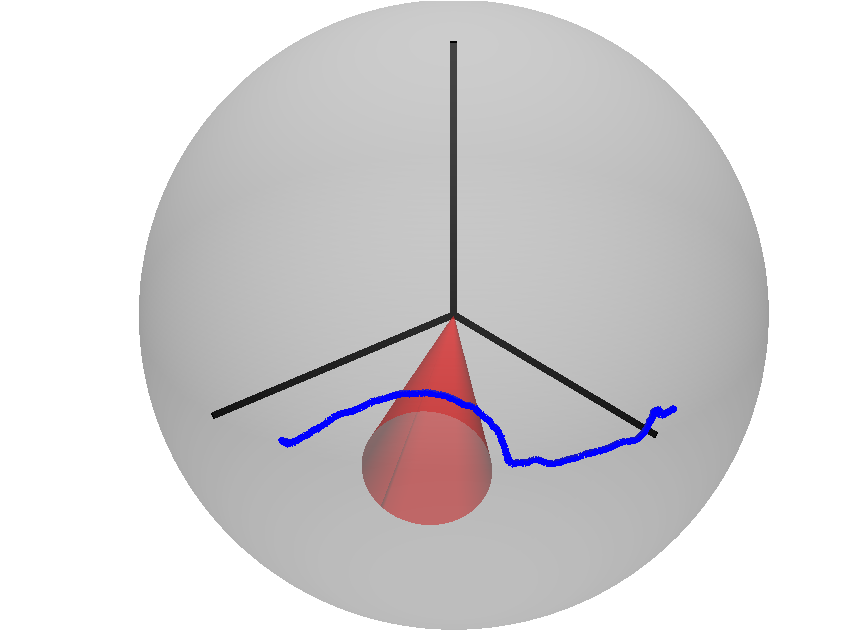
\includegraphics[width=0.3\columnwidth]{traj_exp} }~
    \subfigure[{Angle to constraint } \label{fig:con_angle_exp}]{%% Creator: Matplotlib, PGF backend
%%
%% To include the figure in your LaTeX document, write
%%   \input{<filename>.pgf}
%%
%% Make sure the required packages are loaded in your preamble
%%   \usepackage{pgf}
%%
%% Figures using additional raster images can only be included by \input if
%% they are in the same directory as the main LaTeX file. For loading figures
%% from other directories you can use the `import` package
%%   \usepackage{import}
%% and then include the figures with
%%   \import{<path to file>}{<filename>.pgf}
%%
%% Matplotlib used the following preamble
%%   \usepackage[utf8x]{inputenc}
%%   \usepackage[T1]{fontenc}
%%   \usepackage{siunitx}
%%
\begingroup%
\makeatletter%
\begin{pgfpicture}%
\pgfpathrectangle{\pgfpointorigin}{\pgfqpoint{2.227534in}{1.887367in}}%
\pgfusepath{use as bounding box, clip}%
\begin{pgfscope}%
\pgfsetbuttcap%
\pgfsetmiterjoin%
\definecolor{currentfill}{rgb}{1.000000,1.000000,1.000000}%
\pgfsetfillcolor{currentfill}%
\pgfsetlinewidth{0.000000pt}%
\definecolor{currentstroke}{rgb}{1.000000,1.000000,1.000000}%
\pgfsetstrokecolor{currentstroke}%
\pgfsetdash{}{0pt}%
\pgfpathmoveto{\pgfqpoint{0.000000in}{0.000000in}}%
\pgfpathlineto{\pgfqpoint{2.227534in}{0.000000in}}%
\pgfpathlineto{\pgfqpoint{2.227534in}{1.887367in}}%
\pgfpathlineto{\pgfqpoint{0.000000in}{1.887367in}}%
\pgfpathclose%
\pgfusepath{fill}%
\end{pgfscope}%
\begin{pgfscope}%
\pgfsetbuttcap%
\pgfsetmiterjoin%
\definecolor{currentfill}{rgb}{1.000000,1.000000,1.000000}%
\pgfsetfillcolor{currentfill}%
\pgfsetlinewidth{0.000000pt}%
\definecolor{currentstroke}{rgb}{0.000000,0.000000,0.000000}%
\pgfsetstrokecolor{currentstroke}%
\pgfsetstrokeopacity{0.000000}%
\pgfsetdash{}{0pt}%
\pgfpathmoveto{\pgfqpoint{0.521715in}{0.481986in}}%
\pgfpathlineto{\pgfqpoint{2.107534in}{0.481986in}}%
\pgfpathlineto{\pgfqpoint{2.107534in}{1.767367in}}%
\pgfpathlineto{\pgfqpoint{0.521715in}{1.767367in}}%
\pgfpathclose%
\pgfusepath{fill}%
\end{pgfscope}%
\begin{pgfscope}%
\definecolor{textcolor}{rgb}{0.150000,0.150000,0.150000}%
\pgfsetstrokecolor{textcolor}%
\pgfsetfillcolor{textcolor}%
\pgftext[x=0.592842in,y=0.384764in,,top]{\color{textcolor}\rmfamily\fontsize{8.000000}{9.600000}\selectfont \(\displaystyle 0\)}%
\end{pgfscope}%
\begin{pgfscope}%
\definecolor{textcolor}{rgb}{0.150000,0.150000,0.150000}%
\pgfsetstrokecolor{textcolor}%
\pgfsetfillcolor{textcolor}%
\pgftext[x=1.169853in,y=0.384764in,,top]{\color{textcolor}\rmfamily\fontsize{8.000000}{9.600000}\selectfont \(\displaystyle 5\)}%
\end{pgfscope}%
\begin{pgfscope}%
\definecolor{textcolor}{rgb}{0.150000,0.150000,0.150000}%
\pgfsetstrokecolor{textcolor}%
\pgfsetfillcolor{textcolor}%
\pgftext[x=1.746864in,y=0.384764in,,top]{\color{textcolor}\rmfamily\fontsize{8.000000}{9.600000}\selectfont \(\displaystyle 10\)}%
\end{pgfscope}%
\begin{pgfscope}%
\definecolor{textcolor}{rgb}{0.150000,0.150000,0.150000}%
\pgfsetstrokecolor{textcolor}%
\pgfsetfillcolor{textcolor}%
\pgftext[x=1.314624in,y=0.231084in,,top]{\color{textcolor}\rmfamily\fontsize{8.000000}{9.600000}\selectfont \(\displaystyle t\) (sec)}%
\end{pgfscope}%
\begin{pgfscope}%
\definecolor{textcolor}{rgb}{0.150000,0.150000,0.150000}%
\pgfsetstrokecolor{textcolor}%
\pgfsetfillcolor{textcolor}%
\pgftext[x=0.306435in,y=0.675198in,left,base]{\color{textcolor}\rmfamily\fontsize{8.000000}{9.600000}\selectfont \(\displaystyle 20\)}%
\end{pgfscope}%
\begin{pgfscope}%
\definecolor{textcolor}{rgb}{0.150000,0.150000,0.150000}%
\pgfsetstrokecolor{textcolor}%
\pgfsetfillcolor{textcolor}%
\pgftext[x=0.306435in,y=1.012327in,left,base]{\color{textcolor}\rmfamily\fontsize{8.000000}{9.600000}\selectfont \(\displaystyle 30\)}%
\end{pgfscope}%
\begin{pgfscope}%
\definecolor{textcolor}{rgb}{0.150000,0.150000,0.150000}%
\pgfsetstrokecolor{textcolor}%
\pgfsetfillcolor{textcolor}%
\pgftext[x=0.306435in,y=1.349456in,left,base]{\color{textcolor}\rmfamily\fontsize{8.000000}{9.600000}\selectfont \(\displaystyle 40\)}%
\end{pgfscope}%
\begin{pgfscope}%
\definecolor{textcolor}{rgb}{0.150000,0.150000,0.150000}%
\pgfsetstrokecolor{textcolor}%
\pgfsetfillcolor{textcolor}%
\pgftext[x=0.306435in,y=1.686584in,left,base]{\color{textcolor}\rmfamily\fontsize{8.000000}{9.600000}\selectfont \(\displaystyle 50\)}%
\end{pgfscope}%
\begin{pgfscope}%
\definecolor{textcolor}{rgb}{0.150000,0.150000,0.150000}%
\pgfsetstrokecolor{textcolor}%
\pgfsetfillcolor{textcolor}%
\pgftext[x=0.250880in,y=1.124676in,,bottom,rotate=90.000000]{\color{textcolor}\rmfamily\fontsize{8.000000}{9.600000}\selectfont \(\displaystyle \arccos (r^T R^T v_i)\)}%
\end{pgfscope}%
\begin{pgfscope}%
\pgfpathrectangle{\pgfqpoint{0.521715in}{0.481986in}}{\pgfqpoint{1.585820in}{1.285381in}} %
\pgfusepath{clip}%
\pgfsetroundcap%
\pgfsetroundjoin%
\pgfsetlinewidth{2.007500pt}%
\definecolor{currentstroke}{rgb}{0.298039,0.447059,0.690196}%
\pgfsetstrokecolor{currentstroke}%
\pgfsetdash{}{0pt}%
\pgfpathmoveto{\pgfqpoint{0.593797in}{1.700878in}}%
\pgfpathlineto{\pgfqpoint{0.594026in}{1.700449in}}%
\pgfpathlineto{\pgfqpoint{0.595510in}{1.703596in}}%
\pgfpathlineto{\pgfqpoint{0.595659in}{1.703208in}}%
\pgfpathlineto{\pgfqpoint{0.597766in}{1.706882in}}%
\pgfpathlineto{\pgfqpoint{0.598975in}{1.702896in}}%
\pgfpathlineto{\pgfqpoint{0.599338in}{1.703119in}}%
\pgfpathlineto{\pgfqpoint{0.604066in}{1.701789in}}%
\pgfpathlineto{\pgfqpoint{0.605219in}{1.698330in}}%
\pgfpathlineto{\pgfqpoint{0.605451in}{1.700726in}}%
\pgfpathlineto{\pgfqpoint{0.608433in}{1.704683in}}%
\pgfpathlineto{\pgfqpoint{0.608714in}{1.700886in}}%
\pgfpathlineto{\pgfqpoint{0.610664in}{1.701896in}}%
\pgfpathlineto{\pgfqpoint{0.610938in}{1.700705in}}%
\pgfpathlineto{\pgfqpoint{0.611173in}{1.699115in}}%
\pgfpathlineto{\pgfqpoint{0.611956in}{1.704811in}}%
\pgfpathlineto{\pgfqpoint{0.612454in}{1.701701in}}%
\pgfpathlineto{\pgfqpoint{0.614320in}{1.701307in}}%
\pgfpathlineto{\pgfqpoint{0.615394in}{1.703354in}}%
\pgfpathlineto{\pgfqpoint{0.616687in}{1.702958in}}%
\pgfpathlineto{\pgfqpoint{0.616928in}{1.708940in}}%
\pgfpathlineto{\pgfqpoint{0.617379in}{1.704275in}}%
\pgfpathlineto{\pgfqpoint{0.617379in}{1.704275in}}%
\pgfpathlineto{\pgfqpoint{0.617610in}{1.700258in}}%
\pgfpathlineto{\pgfqpoint{0.618598in}{1.701894in}}%
\pgfpathlineto{\pgfqpoint{0.620276in}{1.701748in}}%
\pgfpathlineto{\pgfqpoint{0.621161in}{1.703701in}}%
\pgfpathlineto{\pgfqpoint{0.622532in}{1.701503in}}%
\pgfpathlineto{\pgfqpoint{0.627618in}{1.701787in}}%
\pgfpathlineto{\pgfqpoint{0.628301in}{1.704953in}}%
\pgfpathlineto{\pgfqpoint{0.629047in}{1.703015in}}%
\pgfpathlineto{\pgfqpoint{0.631655in}{1.705002in}}%
\pgfpathlineto{\pgfqpoint{0.632274in}{1.704154in}}%
\pgfpathlineto{\pgfqpoint{0.632554in}{1.705621in}}%
\pgfpathlineto{\pgfqpoint{0.632787in}{1.705903in}}%
\pgfpathlineto{\pgfqpoint{0.633249in}{1.704056in}}%
\pgfpathlineto{\pgfqpoint{0.633910in}{1.705873in}}%
\pgfpathlineto{\pgfqpoint{0.634562in}{1.708626in}}%
\pgfpathlineto{\pgfqpoint{0.635198in}{1.704091in}}%
\pgfpathlineto{\pgfqpoint{0.635840in}{1.705515in}}%
\pgfpathlineto{\pgfqpoint{0.636046in}{1.706368in}}%
\pgfpathlineto{\pgfqpoint{0.637670in}{1.702597in}}%
\pgfpathlineto{\pgfqpoint{0.638932in}{1.703935in}}%
\pgfpathlineto{\pgfqpoint{0.641877in}{1.700478in}}%
\pgfpathlineto{\pgfqpoint{0.642781in}{1.701631in}}%
\pgfpathlineto{\pgfqpoint{0.643438in}{1.698660in}}%
\pgfpathlineto{\pgfqpoint{0.645959in}{1.700844in}}%
\pgfpathlineto{\pgfqpoint{0.647669in}{1.702380in}}%
\pgfpathlineto{\pgfqpoint{0.647930in}{1.700067in}}%
\pgfpathlineto{\pgfqpoint{0.650758in}{1.700523in}}%
\pgfpathlineto{\pgfqpoint{0.651656in}{1.697945in}}%
\pgfpathlineto{\pgfqpoint{0.651911in}{1.699092in}}%
\pgfpathlineto{\pgfqpoint{0.652281in}{1.698537in}}%
\pgfpathlineto{\pgfqpoint{0.652833in}{1.699332in}}%
\pgfpathlineto{\pgfqpoint{0.653094in}{1.700786in}}%
\pgfpathlineto{\pgfqpoint{0.655622in}{1.694192in}}%
\pgfpathlineto{\pgfqpoint{0.658125in}{1.702774in}}%
\pgfpathlineto{\pgfqpoint{0.658757in}{1.693975in}}%
\pgfpathlineto{\pgfqpoint{0.660746in}{1.694591in}}%
\pgfpathlineto{\pgfqpoint{0.662582in}{1.687555in}}%
\pgfpathlineto{\pgfqpoint{0.663001in}{1.688574in}}%
\pgfpathlineto{\pgfqpoint{0.667552in}{1.684856in}}%
\pgfpathlineto{\pgfqpoint{0.669056in}{1.679123in}}%
\pgfpathlineto{\pgfqpoint{0.669597in}{1.679019in}}%
\pgfpathlineto{\pgfqpoint{0.671325in}{1.674444in}}%
\pgfpathlineto{\pgfqpoint{0.672333in}{1.674936in}}%
\pgfpathlineto{\pgfqpoint{0.674128in}{1.665760in}}%
\pgfpathlineto{\pgfqpoint{0.674539in}{1.676245in}}%
\pgfpathlineto{\pgfqpoint{0.675049in}{1.667512in}}%
\pgfpathlineto{\pgfqpoint{0.678257in}{1.665429in}}%
\pgfpathlineto{\pgfqpoint{0.682212in}{1.658258in}}%
\pgfpathlineto{\pgfqpoint{0.682486in}{1.659574in}}%
\pgfpathlineto{\pgfqpoint{0.683067in}{1.659028in}}%
\pgfpathlineto{\pgfqpoint{0.684581in}{1.657874in}}%
\pgfpathlineto{\pgfqpoint{0.685133in}{1.659459in}}%
\pgfpathlineto{\pgfqpoint{0.686534in}{1.657677in}}%
\pgfpathlineto{\pgfqpoint{0.690746in}{1.656140in}}%
\pgfpathlineto{\pgfqpoint{0.692176in}{1.652960in}}%
\pgfpathlineto{\pgfqpoint{0.695297in}{1.653842in}}%
\pgfpathlineto{\pgfqpoint{0.695812in}{1.651634in}}%
\pgfpathlineto{\pgfqpoint{0.697536in}{1.653879in}}%
\pgfpathlineto{\pgfqpoint{0.698492in}{1.651386in}}%
\pgfpathlineto{\pgfqpoint{0.698752in}{1.652937in}}%
\pgfpathlineto{\pgfqpoint{0.701226in}{1.650213in}}%
\pgfpathlineto{\pgfqpoint{0.701602in}{1.651598in}}%
\pgfpathlineto{\pgfqpoint{0.701918in}{1.650893in}}%
\pgfpathlineto{\pgfqpoint{0.703316in}{1.651414in}}%
\pgfpathlineto{\pgfqpoint{0.703563in}{1.648359in}}%
\pgfpathlineto{\pgfqpoint{0.704860in}{1.650857in}}%
\pgfpathlineto{\pgfqpoint{0.708364in}{1.645145in}}%
\pgfpathlineto{\pgfqpoint{0.708902in}{1.648327in}}%
\pgfpathlineto{\pgfqpoint{0.712533in}{1.648590in}}%
\pgfpathlineto{\pgfqpoint{0.714949in}{1.640786in}}%
\pgfpathlineto{\pgfqpoint{0.717214in}{1.643765in}}%
\pgfpathlineto{\pgfqpoint{0.718676in}{1.642303in}}%
\pgfpathlineto{\pgfqpoint{0.719480in}{1.645631in}}%
\pgfpathlineto{\pgfqpoint{0.720088in}{1.638976in}}%
\pgfpathlineto{\pgfqpoint{0.721018in}{1.639142in}}%
\pgfpathlineto{\pgfqpoint{0.721465in}{1.639242in}}%
\pgfpathlineto{\pgfqpoint{0.721741in}{1.635695in}}%
\pgfpathlineto{\pgfqpoint{0.723068in}{1.637835in}}%
\pgfpathlineto{\pgfqpoint{0.723822in}{1.636203in}}%
\pgfpathlineto{\pgfqpoint{0.724079in}{1.637416in}}%
\pgfpathlineto{\pgfqpoint{0.724636in}{1.637880in}}%
\pgfpathlineto{\pgfqpoint{0.725179in}{1.633244in}}%
\pgfpathlineto{\pgfqpoint{0.725793in}{1.641395in}}%
\pgfpathlineto{\pgfqpoint{0.726362in}{1.634982in}}%
\pgfpathlineto{\pgfqpoint{0.726615in}{1.633287in}}%
\pgfpathlineto{\pgfqpoint{0.727820in}{1.632793in}}%
\pgfpathlineto{\pgfqpoint{0.728527in}{1.634783in}}%
\pgfpathlineto{\pgfqpoint{0.729220in}{1.634524in}}%
\pgfpathlineto{\pgfqpoint{0.729897in}{1.630242in}}%
\pgfpathlineto{\pgfqpoint{0.730343in}{1.631288in}}%
\pgfpathlineto{\pgfqpoint{0.731016in}{1.634153in}}%
\pgfpathlineto{\pgfqpoint{0.734727in}{1.630646in}}%
\pgfpathlineto{\pgfqpoint{0.736798in}{1.632607in}}%
\pgfpathlineto{\pgfqpoint{0.737860in}{1.630234in}}%
\pgfpathlineto{\pgfqpoint{0.738229in}{1.633093in}}%
\pgfpathlineto{\pgfqpoint{0.739715in}{1.629678in}}%
\pgfpathlineto{\pgfqpoint{0.739959in}{1.629798in}}%
\pgfpathlineto{\pgfqpoint{0.742503in}{1.627493in}}%
\pgfpathlineto{\pgfqpoint{0.743096in}{1.623754in}}%
\pgfpathlineto{\pgfqpoint{0.744523in}{1.625235in}}%
\pgfpathlineto{\pgfqpoint{0.745402in}{1.619053in}}%
\pgfpathlineto{\pgfqpoint{0.746094in}{1.619446in}}%
\pgfpathlineto{\pgfqpoint{0.746395in}{1.619350in}}%
\pgfpathlineto{\pgfqpoint{0.746894in}{1.614672in}}%
\pgfpathlineto{\pgfqpoint{0.749141in}{1.614048in}}%
\pgfpathlineto{\pgfqpoint{0.751123in}{1.604491in}}%
\pgfpathlineto{\pgfqpoint{0.752526in}{1.604744in}}%
\pgfpathlineto{\pgfqpoint{0.754266in}{1.591299in}}%
\pgfpathlineto{\pgfqpoint{0.757700in}{1.587208in}}%
\pgfpathlineto{\pgfqpoint{0.759416in}{1.586179in}}%
\pgfpathlineto{\pgfqpoint{0.760643in}{1.584011in}}%
\pgfpathlineto{\pgfqpoint{0.762095in}{1.584435in}}%
\pgfpathlineto{\pgfqpoint{0.762890in}{1.586531in}}%
\pgfpathlineto{\pgfqpoint{0.764737in}{1.582461in}}%
\pgfpathlineto{\pgfqpoint{0.765496in}{1.585147in}}%
\pgfpathlineto{\pgfqpoint{0.768076in}{1.587342in}}%
\pgfpathlineto{\pgfqpoint{0.769090in}{1.582303in}}%
\pgfpathlineto{\pgfqpoint{0.769677in}{1.584635in}}%
\pgfpathlineto{\pgfqpoint{0.771336in}{1.588141in}}%
\pgfpathlineto{\pgfqpoint{0.771854in}{1.587747in}}%
\pgfpathlineto{\pgfqpoint{0.772099in}{1.588536in}}%
\pgfpathlineto{\pgfqpoint{0.773639in}{1.590881in}}%
\pgfpathlineto{\pgfqpoint{0.775456in}{1.591264in}}%
\pgfpathlineto{\pgfqpoint{0.776273in}{1.594797in}}%
\pgfpathlineto{\pgfqpoint{0.776863in}{1.592882in}}%
\pgfpathlineto{\pgfqpoint{0.778401in}{1.589246in}}%
\pgfpathlineto{\pgfqpoint{0.779211in}{1.594682in}}%
\pgfpathlineto{\pgfqpoint{0.780963in}{1.590231in}}%
\pgfpathlineto{\pgfqpoint{0.781487in}{1.591315in}}%
\pgfpathlineto{\pgfqpoint{0.784231in}{1.590300in}}%
\pgfpathlineto{\pgfqpoint{0.785816in}{1.590400in}}%
\pgfpathlineto{\pgfqpoint{0.787174in}{1.587282in}}%
\pgfpathlineto{\pgfqpoint{0.787953in}{1.584596in}}%
\pgfpathlineto{\pgfqpoint{0.793218in}{1.585036in}}%
\pgfpathlineto{\pgfqpoint{0.793580in}{1.582397in}}%
\pgfpathlineto{\pgfqpoint{0.793580in}{1.582397in}}%
\pgfpathlineto{\pgfqpoint{0.793580in}{1.582397in}}%
\pgfpathlineto{\pgfqpoint{0.794000in}{1.585904in}}%
\pgfpathlineto{\pgfqpoint{0.797738in}{1.581340in}}%
\pgfpathlineto{\pgfqpoint{0.798428in}{1.581888in}}%
\pgfpathlineto{\pgfqpoint{0.799538in}{1.583464in}}%
\pgfpathlineto{\pgfqpoint{0.799884in}{1.582695in}}%
\pgfpathlineto{\pgfqpoint{0.801862in}{1.579862in}}%
\pgfpathlineto{\pgfqpoint{0.802494in}{1.581641in}}%
\pgfpathlineto{\pgfqpoint{0.803967in}{1.582044in}}%
\pgfpathlineto{\pgfqpoint{0.804197in}{1.579427in}}%
\pgfpathlineto{\pgfqpoint{0.804902in}{1.580599in}}%
\pgfpathlineto{\pgfqpoint{0.805345in}{1.584617in}}%
\pgfpathlineto{\pgfqpoint{0.806829in}{1.581848in}}%
\pgfpathlineto{\pgfqpoint{0.807805in}{1.583296in}}%
\pgfpathlineto{\pgfqpoint{0.809897in}{1.580257in}}%
\pgfpathlineto{\pgfqpoint{0.810295in}{1.581808in}}%
\pgfpathlineto{\pgfqpoint{0.813643in}{1.579286in}}%
\pgfpathlineto{\pgfqpoint{0.814358in}{1.580071in}}%
\pgfpathlineto{\pgfqpoint{0.818344in}{1.578137in}}%
\pgfpathlineto{\pgfqpoint{0.824807in}{1.576041in}}%
\pgfpathlineto{\pgfqpoint{0.826311in}{1.570846in}}%
\pgfpathlineto{\pgfqpoint{0.826712in}{1.572760in}}%
\pgfpathlineto{\pgfqpoint{0.826966in}{1.573920in}}%
\pgfpathlineto{\pgfqpoint{0.827605in}{1.572994in}}%
\pgfpathlineto{\pgfqpoint{0.828339in}{1.573469in}}%
\pgfpathlineto{\pgfqpoint{0.829468in}{1.571120in}}%
\pgfpathlineto{\pgfqpoint{0.830772in}{1.571676in}}%
\pgfpathlineto{\pgfqpoint{0.832765in}{1.569600in}}%
\pgfpathlineto{\pgfqpoint{0.833476in}{1.569849in}}%
\pgfpathlineto{\pgfqpoint{0.834740in}{1.568022in}}%
\pgfpathlineto{\pgfqpoint{0.834959in}{1.569251in}}%
\pgfpathlineto{\pgfqpoint{0.838506in}{1.565134in}}%
\pgfpathlineto{\pgfqpoint{0.839195in}{1.567349in}}%
\pgfpathlineto{\pgfqpoint{0.839539in}{1.566557in}}%
\pgfpathlineto{\pgfqpoint{0.840804in}{1.566044in}}%
\pgfpathlineto{\pgfqpoint{0.841011in}{1.563696in}}%
\pgfpathlineto{\pgfqpoint{0.842015in}{1.564322in}}%
\pgfpathlineto{\pgfqpoint{0.843671in}{1.561390in}}%
\pgfpathlineto{\pgfqpoint{0.844127in}{1.563132in}}%
\pgfpathlineto{\pgfqpoint{0.847135in}{1.561926in}}%
\pgfpathlineto{\pgfqpoint{0.848242in}{1.563532in}}%
\pgfpathlineto{\pgfqpoint{0.848477in}{1.562136in}}%
\pgfpathlineto{\pgfqpoint{0.851417in}{1.559725in}}%
\pgfpathlineto{\pgfqpoint{0.853924in}{1.561399in}}%
\pgfpathlineto{\pgfqpoint{0.854149in}{1.560881in}}%
\pgfpathlineto{\pgfqpoint{0.856066in}{1.560798in}}%
\pgfpathlineto{\pgfqpoint{0.858627in}{1.559260in}}%
\pgfpathlineto{\pgfqpoint{0.861337in}{1.560053in}}%
\pgfpathlineto{\pgfqpoint{0.862531in}{1.557857in}}%
\pgfpathlineto{\pgfqpoint{0.863681in}{1.559446in}}%
\pgfpathlineto{\pgfqpoint{0.867506in}{1.560383in}}%
\pgfpathlineto{\pgfqpoint{0.868096in}{1.557969in}}%
\pgfpathlineto{\pgfqpoint{0.869273in}{1.557855in}}%
\pgfpathlineto{\pgfqpoint{0.870481in}{1.556959in}}%
\pgfpathlineto{\pgfqpoint{0.870708in}{1.558040in}}%
\pgfpathlineto{\pgfqpoint{0.877443in}{1.549343in}}%
\pgfpathlineto{\pgfqpoint{0.878348in}{1.549900in}}%
\pgfpathlineto{\pgfqpoint{0.879040in}{1.548282in}}%
\pgfpathlineto{\pgfqpoint{0.879491in}{1.550300in}}%
\pgfpathlineto{\pgfqpoint{0.881418in}{1.548491in}}%
\pgfpathlineto{\pgfqpoint{0.881663in}{1.546926in}}%
\pgfpathlineto{\pgfqpoint{0.882729in}{1.547175in}}%
\pgfpathlineto{\pgfqpoint{0.883291in}{1.549243in}}%
\pgfpathlineto{\pgfqpoint{0.883550in}{1.548638in}}%
\pgfpathlineto{\pgfqpoint{0.889648in}{1.548514in}}%
\pgfpathlineto{\pgfqpoint{0.889882in}{1.545702in}}%
\pgfpathlineto{\pgfqpoint{0.890301in}{1.547842in}}%
\pgfpathlineto{\pgfqpoint{0.892846in}{1.548723in}}%
\pgfpathlineto{\pgfqpoint{0.895499in}{1.545885in}}%
\pgfpathlineto{\pgfqpoint{0.897777in}{1.547132in}}%
\pgfpathlineto{\pgfqpoint{0.899761in}{1.545556in}}%
\pgfpathlineto{\pgfqpoint{0.900573in}{1.548836in}}%
\pgfpathlineto{\pgfqpoint{0.901663in}{1.547895in}}%
\pgfpathlineto{\pgfqpoint{0.904213in}{1.550800in}}%
\pgfpathlineto{\pgfqpoint{0.904894in}{1.548737in}}%
\pgfpathlineto{\pgfqpoint{0.905659in}{1.552202in}}%
\pgfpathlineto{\pgfqpoint{0.906227in}{1.550681in}}%
\pgfpathlineto{\pgfqpoint{0.907501in}{1.550675in}}%
\pgfpathlineto{\pgfqpoint{0.907736in}{1.550111in}}%
\pgfpathlineto{\pgfqpoint{0.907969in}{1.550392in}}%
\pgfpathlineto{\pgfqpoint{0.909034in}{1.550868in}}%
\pgfpathlineto{\pgfqpoint{0.909961in}{1.547841in}}%
\pgfpathlineto{\pgfqpoint{0.910207in}{1.550740in}}%
\pgfpathlineto{\pgfqpoint{0.910998in}{1.550258in}}%
\pgfpathlineto{\pgfqpoint{0.912319in}{1.550954in}}%
\pgfpathlineto{\pgfqpoint{0.912521in}{1.547459in}}%
\pgfpathlineto{\pgfqpoint{0.913008in}{1.548567in}}%
\pgfpathlineto{\pgfqpoint{0.914086in}{1.547846in}}%
\pgfpathlineto{\pgfqpoint{0.915533in}{1.547004in}}%
\pgfpathlineto{\pgfqpoint{0.918885in}{1.544816in}}%
\pgfpathlineto{\pgfqpoint{0.919399in}{1.547201in}}%
\pgfpathlineto{\pgfqpoint{0.919882in}{1.546834in}}%
\pgfpathlineto{\pgfqpoint{0.920285in}{1.545776in}}%
\pgfpathlineto{\pgfqpoint{0.923377in}{1.546360in}}%
\pgfpathlineto{\pgfqpoint{0.924077in}{1.545846in}}%
\pgfpathlineto{\pgfqpoint{0.924925in}{1.546603in}}%
\pgfpathlineto{\pgfqpoint{0.926857in}{1.546388in}}%
\pgfpathlineto{\pgfqpoint{0.927490in}{1.543819in}}%
\pgfpathlineto{\pgfqpoint{0.927961in}{1.545394in}}%
\pgfpathlineto{\pgfqpoint{0.931363in}{1.545002in}}%
\pgfpathlineto{\pgfqpoint{0.932522in}{1.542974in}}%
\pgfpathlineto{\pgfqpoint{0.933258in}{1.543197in}}%
\pgfpathlineto{\pgfqpoint{0.933818in}{1.545379in}}%
\pgfpathlineto{\pgfqpoint{0.935315in}{1.544688in}}%
\pgfpathlineto{\pgfqpoint{0.936659in}{1.541117in}}%
\pgfpathlineto{\pgfqpoint{0.937125in}{1.541614in}}%
\pgfpathlineto{\pgfqpoint{0.937773in}{1.540770in}}%
\pgfpathlineto{\pgfqpoint{0.944231in}{1.536553in}}%
\pgfpathlineto{\pgfqpoint{0.945881in}{1.532839in}}%
\pgfpathlineto{\pgfqpoint{0.946259in}{1.529557in}}%
\pgfpathlineto{\pgfqpoint{0.947105in}{1.531573in}}%
\pgfpathlineto{\pgfqpoint{0.949147in}{1.530398in}}%
\pgfpathlineto{\pgfqpoint{0.949391in}{1.531647in}}%
\pgfpathlineto{\pgfqpoint{0.949391in}{1.531647in}}%
\pgfpathlineto{\pgfqpoint{0.949391in}{1.531647in}}%
\pgfpathlineto{\pgfqpoint{0.949890in}{1.529708in}}%
\pgfpathlineto{\pgfqpoint{0.950813in}{1.530218in}}%
\pgfpathlineto{\pgfqpoint{0.957807in}{1.528429in}}%
\pgfpathlineto{\pgfqpoint{0.958335in}{1.529974in}}%
\pgfpathlineto{\pgfqpoint{0.959004in}{1.529447in}}%
\pgfpathlineto{\pgfqpoint{0.963171in}{1.531679in}}%
\pgfpathlineto{\pgfqpoint{0.966316in}{1.532775in}}%
\pgfpathlineto{\pgfqpoint{0.969969in}{1.530782in}}%
\pgfpathlineto{\pgfqpoint{0.972042in}{1.532172in}}%
\pgfpathlineto{\pgfqpoint{0.973770in}{1.531905in}}%
\pgfpathlineto{\pgfqpoint{0.974574in}{1.531842in}}%
\pgfpathlineto{\pgfqpoint{0.975026in}{1.529543in}}%
\pgfpathlineto{\pgfqpoint{0.975274in}{1.530491in}}%
\pgfpathlineto{\pgfqpoint{0.976477in}{1.531588in}}%
\pgfpathlineto{\pgfqpoint{0.979601in}{1.530149in}}%
\pgfpathlineto{\pgfqpoint{0.980850in}{1.531746in}}%
\pgfpathlineto{\pgfqpoint{0.982710in}{1.528736in}}%
\pgfpathlineto{\pgfqpoint{0.983091in}{1.531045in}}%
\pgfpathlineto{\pgfqpoint{0.983561in}{1.530567in}}%
\pgfpathlineto{\pgfqpoint{0.985344in}{1.528801in}}%
\pgfpathlineto{\pgfqpoint{0.987105in}{1.531581in}}%
\pgfpathlineto{\pgfqpoint{0.989951in}{1.528854in}}%
\pgfpathlineto{\pgfqpoint{0.990611in}{1.526669in}}%
\pgfpathlineto{\pgfqpoint{0.990828in}{1.528573in}}%
\pgfpathlineto{\pgfqpoint{0.994191in}{1.528264in}}%
\pgfpathlineto{\pgfqpoint{0.994588in}{1.526006in}}%
\pgfpathlineto{\pgfqpoint{0.995098in}{1.527982in}}%
\pgfpathlineto{\pgfqpoint{0.997325in}{1.525203in}}%
\pgfpathlineto{\pgfqpoint{0.998535in}{1.525251in}}%
\pgfpathlineto{\pgfqpoint{0.999350in}{1.528020in}}%
\pgfpathlineto{\pgfqpoint{0.999859in}{1.527573in}}%
\pgfpathlineto{\pgfqpoint{1.000887in}{1.523848in}}%
\pgfpathlineto{\pgfqpoint{1.002539in}{1.525211in}}%
\pgfpathlineto{\pgfqpoint{1.004406in}{1.524413in}}%
\pgfpathlineto{\pgfqpoint{1.004853in}{1.524981in}}%
\pgfpathlineto{\pgfqpoint{1.008488in}{1.523603in}}%
\pgfpathlineto{\pgfqpoint{1.009549in}{1.524967in}}%
\pgfpathlineto{\pgfqpoint{1.011317in}{1.520835in}}%
\pgfpathlineto{\pgfqpoint{1.013241in}{1.522748in}}%
\pgfpathlineto{\pgfqpoint{1.013938in}{1.521231in}}%
\pgfpathlineto{\pgfqpoint{1.017667in}{1.518887in}}%
\pgfpathlineto{\pgfqpoint{1.020593in}{1.521806in}}%
\pgfpathlineto{\pgfqpoint{1.021222in}{1.520723in}}%
\pgfpathlineto{\pgfqpoint{1.022358in}{1.517068in}}%
\pgfpathlineto{\pgfqpoint{1.026602in}{1.520675in}}%
\pgfpathlineto{\pgfqpoint{1.026923in}{1.517900in}}%
\pgfpathlineto{\pgfqpoint{1.029022in}{1.519986in}}%
\pgfpathlineto{\pgfqpoint{1.029252in}{1.516834in}}%
\pgfpathlineto{\pgfqpoint{1.030213in}{1.517887in}}%
\pgfpathlineto{\pgfqpoint{1.031701in}{1.517228in}}%
\pgfpathlineto{\pgfqpoint{1.033003in}{1.516411in}}%
\pgfpathlineto{\pgfqpoint{1.034310in}{1.517476in}}%
\pgfpathlineto{\pgfqpoint{1.036703in}{1.516518in}}%
\pgfpathlineto{\pgfqpoint{1.037606in}{1.514188in}}%
\pgfpathlineto{\pgfqpoint{1.038300in}{1.514810in}}%
\pgfpathlineto{\pgfqpoint{1.038996in}{1.517712in}}%
\pgfpathlineto{\pgfqpoint{1.040871in}{1.517035in}}%
\pgfpathlineto{\pgfqpoint{1.042835in}{1.514520in}}%
\pgfpathlineto{\pgfqpoint{1.046638in}{1.515265in}}%
\pgfpathlineto{\pgfqpoint{1.047362in}{1.514479in}}%
\pgfpathlineto{\pgfqpoint{1.048139in}{1.518570in}}%
\pgfpathlineto{\pgfqpoint{1.048682in}{1.516282in}}%
\pgfpathlineto{\pgfqpoint{1.049794in}{1.516427in}}%
\pgfpathlineto{\pgfqpoint{1.053771in}{1.514958in}}%
\pgfpathlineto{\pgfqpoint{1.054111in}{1.516503in}}%
\pgfpathlineto{\pgfqpoint{1.054339in}{1.515996in}}%
\pgfpathlineto{\pgfqpoint{1.055564in}{1.517241in}}%
\pgfpathlineto{\pgfqpoint{1.056985in}{1.514338in}}%
\pgfpathlineto{\pgfqpoint{1.059982in}{1.516296in}}%
\pgfpathlineto{\pgfqpoint{1.060511in}{1.513714in}}%
\pgfpathlineto{\pgfqpoint{1.060785in}{1.515164in}}%
\pgfpathlineto{\pgfqpoint{1.062602in}{1.516297in}}%
\pgfpathlineto{\pgfqpoint{1.063531in}{1.514748in}}%
\pgfpathlineto{\pgfqpoint{1.064186in}{1.515922in}}%
\pgfpathlineto{\pgfqpoint{1.064920in}{1.513524in}}%
\pgfpathlineto{\pgfqpoint{1.065444in}{1.516177in}}%
\pgfpathlineto{\pgfqpoint{1.066042in}{1.515989in}}%
\pgfpathlineto{\pgfqpoint{1.074110in}{1.513501in}}%
\pgfpathlineto{\pgfqpoint{1.076585in}{1.514920in}}%
\pgfpathlineto{\pgfqpoint{1.077277in}{1.510473in}}%
\pgfpathlineto{\pgfqpoint{1.077767in}{1.511536in}}%
\pgfpathlineto{\pgfqpoint{1.077996in}{1.513677in}}%
\pgfpathlineto{\pgfqpoint{1.078228in}{1.512603in}}%
\pgfpathlineto{\pgfqpoint{1.079454in}{1.513752in}}%
\pgfpathlineto{\pgfqpoint{1.081133in}{1.510851in}}%
\pgfpathlineto{\pgfqpoint{1.081618in}{1.511202in}}%
\pgfpathlineto{\pgfqpoint{1.082508in}{1.513366in}}%
\pgfpathlineto{\pgfqpoint{1.083925in}{1.510516in}}%
\pgfpathlineto{\pgfqpoint{1.084931in}{1.508309in}}%
\pgfpathlineto{\pgfqpoint{1.088052in}{1.510537in}}%
\pgfpathlineto{\pgfqpoint{1.088775in}{1.509243in}}%
\pgfpathlineto{\pgfqpoint{1.089324in}{1.510308in}}%
\pgfpathlineto{\pgfqpoint{1.089586in}{1.509238in}}%
\pgfpathlineto{\pgfqpoint{1.090902in}{1.509727in}}%
\pgfpathlineto{\pgfqpoint{1.093123in}{1.508227in}}%
\pgfpathlineto{\pgfqpoint{1.093606in}{1.510297in}}%
\pgfpathlineto{\pgfqpoint{1.094352in}{1.508754in}}%
\pgfpathlineto{\pgfqpoint{1.095895in}{1.508075in}}%
\pgfpathlineto{\pgfqpoint{1.097497in}{1.505275in}}%
\pgfpathlineto{\pgfqpoint{1.098546in}{1.505007in}}%
\pgfpathlineto{\pgfqpoint{1.108120in}{1.475489in}}%
\pgfpathlineto{\pgfqpoint{1.113384in}{1.444230in}}%
\pgfpathlineto{\pgfqpoint{1.114298in}{1.439528in}}%
\pgfpathlineto{\pgfqpoint{1.114820in}{1.413023in}}%
\pgfpathlineto{\pgfqpoint{1.116580in}{1.409356in}}%
\pgfpathlineto{\pgfqpoint{1.118582in}{1.373720in}}%
\pgfpathlineto{\pgfqpoint{1.121079in}{1.368259in}}%
\pgfpathlineto{\pgfqpoint{1.123081in}{1.337731in}}%
\pgfpathlineto{\pgfqpoint{1.124670in}{1.315816in}}%
\pgfpathlineto{\pgfqpoint{1.126325in}{1.286093in}}%
\pgfpathlineto{\pgfqpoint{1.133033in}{1.204342in}}%
\pgfpathlineto{\pgfqpoint{1.137619in}{1.155428in}}%
\pgfpathlineto{\pgfqpoint{1.145124in}{1.086853in}}%
\pgfpathlineto{\pgfqpoint{1.146439in}{1.086900in}}%
\pgfpathlineto{\pgfqpoint{1.147897in}{1.070605in}}%
\pgfpathlineto{\pgfqpoint{1.150688in}{1.055334in}}%
\pgfpathlineto{\pgfqpoint{1.152288in}{1.038961in}}%
\pgfpathlineto{\pgfqpoint{1.156355in}{1.000545in}}%
\pgfpathlineto{\pgfqpoint{1.157264in}{0.997725in}}%
\pgfpathlineto{\pgfqpoint{1.162943in}{0.937023in}}%
\pgfpathlineto{\pgfqpoint{1.169581in}{0.931593in}}%
\pgfpathlineto{\pgfqpoint{1.170319in}{0.896697in}}%
\pgfpathlineto{\pgfqpoint{1.171500in}{0.894275in}}%
\pgfpathlineto{\pgfqpoint{1.174814in}{0.866685in}}%
\pgfpathlineto{\pgfqpoint{1.175645in}{0.857094in}}%
\pgfpathlineto{\pgfqpoint{1.177746in}{0.852068in}}%
\pgfpathlineto{\pgfqpoint{1.178087in}{0.841873in}}%
\pgfpathlineto{\pgfqpoint{1.180289in}{0.829551in}}%
\pgfpathlineto{\pgfqpoint{1.181791in}{0.806478in}}%
\pgfpathlineto{\pgfqpoint{1.197172in}{0.726800in}}%
\pgfpathlineto{\pgfqpoint{1.198365in}{0.713457in}}%
\pgfpathlineto{\pgfqpoint{1.207799in}{0.656318in}}%
\pgfpathlineto{\pgfqpoint{1.209149in}{0.653857in}}%
\pgfpathlineto{\pgfqpoint{1.213891in}{0.618886in}}%
\pgfpathlineto{\pgfqpoint{1.214815in}{0.615619in}}%
\pgfpathlineto{\pgfqpoint{1.218550in}{0.602350in}}%
\pgfpathlineto{\pgfqpoint{1.219548in}{0.597212in}}%
\pgfpathlineto{\pgfqpoint{1.220929in}{0.597612in}}%
\pgfpathlineto{\pgfqpoint{1.222409in}{0.591690in}}%
\pgfpathlineto{\pgfqpoint{1.224249in}{0.586239in}}%
\pgfpathlineto{\pgfqpoint{1.224714in}{0.582023in}}%
\pgfpathlineto{\pgfqpoint{1.225393in}{0.583337in}}%
\pgfpathlineto{\pgfqpoint{1.225960in}{0.584737in}}%
\pgfpathlineto{\pgfqpoint{1.228135in}{0.573815in}}%
\pgfpathlineto{\pgfqpoint{1.229820in}{0.568647in}}%
\pgfpathlineto{\pgfqpoint{1.230906in}{0.569661in}}%
\pgfpathlineto{\pgfqpoint{1.231324in}{0.569778in}}%
\pgfpathlineto{\pgfqpoint{1.232756in}{0.566575in}}%
\pgfpathlineto{\pgfqpoint{1.239022in}{0.563218in}}%
\pgfpathlineto{\pgfqpoint{1.240376in}{0.558033in}}%
\pgfpathlineto{\pgfqpoint{1.242271in}{0.560421in}}%
\pgfpathlineto{\pgfqpoint{1.243018in}{0.559583in}}%
\pgfpathlineto{\pgfqpoint{1.245277in}{0.559507in}}%
\pgfpathlineto{\pgfqpoint{1.247502in}{0.554985in}}%
\pgfpathlineto{\pgfqpoint{1.248478in}{0.558184in}}%
\pgfpathlineto{\pgfqpoint{1.249399in}{0.555362in}}%
\pgfpathlineto{\pgfqpoint{1.250110in}{0.555707in}}%
\pgfpathlineto{\pgfqpoint{1.251481in}{0.555632in}}%
\pgfpathlineto{\pgfqpoint{1.253170in}{0.551597in}}%
\pgfpathlineto{\pgfqpoint{1.254398in}{0.554608in}}%
\pgfpathlineto{\pgfqpoint{1.255230in}{0.553757in}}%
\pgfpathlineto{\pgfqpoint{1.255962in}{0.552835in}}%
\pgfpathlineto{\pgfqpoint{1.256132in}{0.554709in}}%
\pgfpathlineto{\pgfqpoint{1.256379in}{0.553669in}}%
\pgfpathlineto{\pgfqpoint{1.257107in}{0.549096in}}%
\pgfpathlineto{\pgfqpoint{1.258754in}{0.552870in}}%
\pgfpathlineto{\pgfqpoint{1.261150in}{0.553057in}}%
\pgfpathlineto{\pgfqpoint{1.261899in}{0.554163in}}%
\pgfpathlineto{\pgfqpoint{1.262128in}{0.552587in}}%
\pgfpathlineto{\pgfqpoint{1.264721in}{0.548881in}}%
\pgfpathlineto{\pgfqpoint{1.265550in}{0.550763in}}%
\pgfpathlineto{\pgfqpoint{1.266849in}{0.550406in}}%
\pgfpathlineto{\pgfqpoint{1.268094in}{0.553789in}}%
\pgfpathlineto{\pgfqpoint{1.268957in}{0.551886in}}%
\pgfpathlineto{\pgfqpoint{1.270336in}{0.550079in}}%
\pgfpathlineto{\pgfqpoint{1.270837in}{0.551171in}}%
\pgfpathlineto{\pgfqpoint{1.273401in}{0.546913in}}%
\pgfpathlineto{\pgfqpoint{1.274539in}{0.549442in}}%
\pgfpathlineto{\pgfqpoint{1.276880in}{0.545633in}}%
\pgfpathlineto{\pgfqpoint{1.278458in}{0.544478in}}%
\pgfpathlineto{\pgfqpoint{1.278699in}{0.545433in}}%
\pgfpathlineto{\pgfqpoint{1.280943in}{0.546410in}}%
\pgfpathlineto{\pgfqpoint{1.282480in}{0.541583in}}%
\pgfpathlineto{\pgfqpoint{1.282946in}{0.543342in}}%
\pgfpathlineto{\pgfqpoint{1.283203in}{0.543585in}}%
\pgfpathlineto{\pgfqpoint{1.284426in}{0.542105in}}%
\pgfpathlineto{\pgfqpoint{1.285091in}{0.545746in}}%
\pgfpathlineto{\pgfqpoint{1.287066in}{0.543366in}}%
\pgfpathlineto{\pgfqpoint{1.287943in}{0.544273in}}%
\pgfpathlineto{\pgfqpoint{1.288552in}{0.542011in}}%
\pgfpathlineto{\pgfqpoint{1.291331in}{0.546394in}}%
\pgfpathlineto{\pgfqpoint{1.292442in}{0.544091in}}%
\pgfpathlineto{\pgfqpoint{1.293139in}{0.545151in}}%
\pgfpathlineto{\pgfqpoint{1.293886in}{0.545982in}}%
\pgfpathlineto{\pgfqpoint{1.294120in}{0.548429in}}%
\pgfpathlineto{\pgfqpoint{1.295123in}{0.547260in}}%
\pgfpathlineto{\pgfqpoint{1.296409in}{0.548640in}}%
\pgfpathlineto{\pgfqpoint{1.296929in}{0.545829in}}%
\pgfpathlineto{\pgfqpoint{1.297862in}{0.545991in}}%
\pgfpathlineto{\pgfqpoint{1.298525in}{0.547484in}}%
\pgfpathlineto{\pgfqpoint{1.299227in}{0.546386in}}%
\pgfpathlineto{\pgfqpoint{1.299923in}{0.547879in}}%
\pgfpathlineto{\pgfqpoint{1.300167in}{0.544787in}}%
\pgfpathlineto{\pgfqpoint{1.302114in}{0.547558in}}%
\pgfpathlineto{\pgfqpoint{1.302824in}{0.546844in}}%
\pgfpathlineto{\pgfqpoint{1.305664in}{0.548806in}}%
\pgfpathlineto{\pgfqpoint{1.306691in}{0.547204in}}%
\pgfpathlineto{\pgfqpoint{1.307596in}{0.543853in}}%
\pgfpathlineto{\pgfqpoint{1.309154in}{0.545433in}}%
\pgfpathlineto{\pgfqpoint{1.310410in}{0.542045in}}%
\pgfpathlineto{\pgfqpoint{1.316913in}{0.544570in}}%
\pgfpathlineto{\pgfqpoint{1.317177in}{0.545677in}}%
\pgfpathlineto{\pgfqpoint{1.318268in}{0.540413in}}%
\pgfpathlineto{\pgfqpoint{1.318506in}{0.543150in}}%
\pgfpathlineto{\pgfqpoint{1.319796in}{0.542653in}}%
\pgfpathlineto{\pgfqpoint{1.321842in}{0.545452in}}%
\pgfpathlineto{\pgfqpoint{1.323002in}{0.542818in}}%
\pgfpathlineto{\pgfqpoint{1.324289in}{0.546256in}}%
\pgfpathlineto{\pgfqpoint{1.325551in}{0.543444in}}%
\pgfpathlineto{\pgfqpoint{1.326031in}{0.544958in}}%
\pgfpathlineto{\pgfqpoint{1.327475in}{0.544427in}}%
\pgfpathlineto{\pgfqpoint{1.327733in}{0.542965in}}%
\pgfpathlineto{\pgfqpoint{1.329217in}{0.543736in}}%
\pgfpathlineto{\pgfqpoint{1.330075in}{0.547338in}}%
\pgfpathlineto{\pgfqpoint{1.330694in}{0.543690in}}%
\pgfpathlineto{\pgfqpoint{1.330992in}{0.545861in}}%
\pgfpathlineto{\pgfqpoint{1.333124in}{0.548836in}}%
\pgfpathlineto{\pgfqpoint{1.333610in}{0.548402in}}%
\pgfpathlineto{\pgfqpoint{1.333839in}{0.545480in}}%
\pgfpathlineto{\pgfqpoint{1.335113in}{0.546572in}}%
\pgfpathlineto{\pgfqpoint{1.335863in}{0.545707in}}%
\pgfpathlineto{\pgfqpoint{1.337618in}{0.548312in}}%
\pgfpathlineto{\pgfqpoint{1.340776in}{0.545879in}}%
\pgfpathlineto{\pgfqpoint{1.341005in}{0.548927in}}%
\pgfpathlineto{\pgfqpoint{1.341716in}{0.546122in}}%
\pgfpathlineto{\pgfqpoint{1.342161in}{0.547973in}}%
\pgfpathlineto{\pgfqpoint{1.342628in}{0.547745in}}%
\pgfpathlineto{\pgfqpoint{1.343615in}{0.543621in}}%
\pgfpathlineto{\pgfqpoint{1.344464in}{0.545007in}}%
\pgfpathlineto{\pgfqpoint{1.345461in}{0.546403in}}%
\pgfpathlineto{\pgfqpoint{1.346136in}{0.545458in}}%
\pgfpathlineto{\pgfqpoint{1.349008in}{0.546126in}}%
\pgfpathlineto{\pgfqpoint{1.350076in}{0.546298in}}%
\pgfpathlineto{\pgfqpoint{1.350539in}{0.548071in}}%
\pgfpathlineto{\pgfqpoint{1.351278in}{0.547665in}}%
\pgfpathlineto{\pgfqpoint{1.351853in}{0.545443in}}%
\pgfpathlineto{\pgfqpoint{1.352528in}{0.545690in}}%
\pgfpathlineto{\pgfqpoint{1.353245in}{0.548711in}}%
\pgfpathlineto{\pgfqpoint{1.354638in}{0.546515in}}%
\pgfpathlineto{\pgfqpoint{1.356631in}{0.548576in}}%
\pgfpathlineto{\pgfqpoint{1.357060in}{0.547802in}}%
\pgfpathlineto{\pgfqpoint{1.357910in}{0.553585in}}%
\pgfpathlineto{\pgfqpoint{1.359523in}{0.555264in}}%
\pgfpathlineto{\pgfqpoint{1.359918in}{0.551534in}}%
\pgfpathlineto{\pgfqpoint{1.363576in}{0.551940in}}%
\pgfpathlineto{\pgfqpoint{1.363804in}{0.550428in}}%
\pgfpathlineto{\pgfqpoint{1.366098in}{0.553869in}}%
\pgfpathlineto{\pgfqpoint{1.367757in}{0.556484in}}%
\pgfpathlineto{\pgfqpoint{1.370410in}{0.555037in}}%
\pgfpathlineto{\pgfqpoint{1.373554in}{0.557577in}}%
\pgfpathlineto{\pgfqpoint{1.373830in}{0.556057in}}%
\pgfpathlineto{\pgfqpoint{1.374584in}{0.557663in}}%
\pgfpathlineto{\pgfqpoint{1.375874in}{0.555702in}}%
\pgfpathlineto{\pgfqpoint{1.377619in}{0.555509in}}%
\pgfpathlineto{\pgfqpoint{1.378155in}{0.557943in}}%
\pgfpathlineto{\pgfqpoint{1.378416in}{0.556068in}}%
\pgfpathlineto{\pgfqpoint{1.379599in}{0.557624in}}%
\pgfpathlineto{\pgfqpoint{1.381510in}{0.554351in}}%
\pgfpathlineto{\pgfqpoint{1.387516in}{0.553158in}}%
\pgfpathlineto{\pgfqpoint{1.388541in}{0.550659in}}%
\pgfpathlineto{\pgfqpoint{1.389660in}{0.552320in}}%
\pgfpathlineto{\pgfqpoint{1.391272in}{0.549202in}}%
\pgfpathlineto{\pgfqpoint{1.393565in}{0.549549in}}%
\pgfpathlineto{\pgfqpoint{1.394924in}{0.548678in}}%
\pgfpathlineto{\pgfqpoint{1.396683in}{0.552078in}}%
\pgfpathlineto{\pgfqpoint{1.397674in}{0.550375in}}%
\pgfpathlineto{\pgfqpoint{1.397930in}{0.552274in}}%
\pgfpathlineto{\pgfqpoint{1.398423in}{0.551262in}}%
\pgfpathlineto{\pgfqpoint{1.406419in}{0.556697in}}%
\pgfpathlineto{\pgfqpoint{1.409799in}{0.551835in}}%
\pgfpathlineto{\pgfqpoint{1.410055in}{0.552422in}}%
\pgfpathlineto{\pgfqpoint{1.410055in}{0.552422in}}%
\pgfpathlineto{\pgfqpoint{1.410055in}{0.552422in}}%
\pgfpathlineto{\pgfqpoint{1.410302in}{0.551462in}}%
\pgfpathlineto{\pgfqpoint{1.411992in}{0.553082in}}%
\pgfpathlineto{\pgfqpoint{1.413532in}{0.551333in}}%
\pgfpathlineto{\pgfqpoint{1.414943in}{0.551148in}}%
\pgfpathlineto{\pgfqpoint{1.415386in}{0.549224in}}%
\pgfpathlineto{\pgfqpoint{1.420122in}{0.554979in}}%
\pgfpathlineto{\pgfqpoint{1.422216in}{0.552691in}}%
\pgfpathlineto{\pgfqpoint{1.422708in}{0.552327in}}%
\pgfpathlineto{\pgfqpoint{1.424113in}{0.555835in}}%
\pgfpathlineto{\pgfqpoint{1.424678in}{0.555451in}}%
\pgfpathlineto{\pgfqpoint{1.425151in}{0.554727in}}%
\pgfpathlineto{\pgfqpoint{1.426870in}{0.556041in}}%
\pgfpathlineto{\pgfqpoint{1.428195in}{0.554235in}}%
\pgfpathlineto{\pgfqpoint{1.429541in}{0.555912in}}%
\pgfpathlineto{\pgfqpoint{1.431450in}{0.563014in}}%
\pgfpathlineto{\pgfqpoint{1.433700in}{0.556481in}}%
\pgfpathlineto{\pgfqpoint{1.433914in}{0.558755in}}%
\pgfpathlineto{\pgfqpoint{1.434405in}{0.557949in}}%
\pgfpathlineto{\pgfqpoint{1.435787in}{0.557392in}}%
\pgfpathlineto{\pgfqpoint{1.437802in}{0.550777in}}%
\pgfpathlineto{\pgfqpoint{1.440156in}{0.549649in}}%
\pgfpathlineto{\pgfqpoint{1.441726in}{0.546955in}}%
\pgfpathlineto{\pgfqpoint{1.442213in}{0.544949in}}%
\pgfpathlineto{\pgfqpoint{1.442719in}{0.545965in}}%
\pgfpathlineto{\pgfqpoint{1.444192in}{0.546796in}}%
\pgfpathlineto{\pgfqpoint{1.445687in}{0.544609in}}%
\pgfpathlineto{\pgfqpoint{1.448885in}{0.549448in}}%
\pgfpathlineto{\pgfqpoint{1.450390in}{0.549063in}}%
\pgfpathlineto{\pgfqpoint{1.453695in}{0.552561in}}%
\pgfpathlineto{\pgfqpoint{1.454092in}{0.554731in}}%
\pgfpathlineto{\pgfqpoint{1.454773in}{0.553077in}}%
\pgfpathlineto{\pgfqpoint{1.455764in}{0.551878in}}%
\pgfpathlineto{\pgfqpoint{1.458444in}{0.559902in}}%
\pgfpathlineto{\pgfqpoint{1.459221in}{0.558761in}}%
\pgfpathlineto{\pgfqpoint{1.459681in}{0.561106in}}%
\pgfpathlineto{\pgfqpoint{1.459681in}{0.561106in}}%
\pgfpathlineto{\pgfqpoint{1.459681in}{0.561106in}}%
\pgfpathlineto{\pgfqpoint{1.461071in}{0.556969in}}%
\pgfpathlineto{\pgfqpoint{1.463242in}{0.561655in}}%
\pgfpathlineto{\pgfqpoint{1.463979in}{0.560373in}}%
\pgfpathlineto{\pgfqpoint{1.464959in}{0.561330in}}%
\pgfpathlineto{\pgfqpoint{1.466895in}{0.557996in}}%
\pgfpathlineto{\pgfqpoint{1.467365in}{0.558077in}}%
\pgfpathlineto{\pgfqpoint{1.467823in}{0.560599in}}%
\pgfpathlineto{\pgfqpoint{1.470248in}{0.560939in}}%
\pgfpathlineto{\pgfqpoint{1.471571in}{0.563527in}}%
\pgfpathlineto{\pgfqpoint{1.472145in}{0.563155in}}%
\pgfpathlineto{\pgfqpoint{1.473058in}{0.561804in}}%
\pgfpathlineto{\pgfqpoint{1.474322in}{0.561281in}}%
\pgfpathlineto{\pgfqpoint{1.476040in}{0.565001in}}%
\pgfpathlineto{\pgfqpoint{1.477551in}{0.561047in}}%
\pgfpathlineto{\pgfqpoint{1.478156in}{0.561653in}}%
\pgfpathlineto{\pgfqpoint{1.480321in}{0.557834in}}%
\pgfpathlineto{\pgfqpoint{1.480831in}{0.559612in}}%
\pgfpathlineto{\pgfqpoint{1.481090in}{0.560887in}}%
\pgfpathlineto{\pgfqpoint{1.481313in}{0.560741in}}%
\pgfpathlineto{\pgfqpoint{1.483459in}{0.561837in}}%
\pgfpathlineto{\pgfqpoint{1.486642in}{0.561819in}}%
\pgfpathlineto{\pgfqpoint{1.487056in}{0.563816in}}%
\pgfpathlineto{\pgfqpoint{1.487480in}{0.560109in}}%
\pgfpathlineto{\pgfqpoint{1.491875in}{0.569330in}}%
\pgfpathlineto{\pgfqpoint{1.493375in}{0.570377in}}%
\pgfpathlineto{\pgfqpoint{1.494389in}{0.573336in}}%
\pgfpathlineto{\pgfqpoint{1.494908in}{0.571078in}}%
\pgfpathlineto{\pgfqpoint{1.495461in}{0.573350in}}%
\pgfpathlineto{\pgfqpoint{1.497760in}{0.573555in}}%
\pgfpathlineto{\pgfqpoint{1.499513in}{0.574875in}}%
\pgfpathlineto{\pgfqpoint{1.502133in}{0.573658in}}%
\pgfpathlineto{\pgfqpoint{1.503598in}{0.577499in}}%
\pgfpathlineto{\pgfqpoint{1.504654in}{0.581622in}}%
\pgfpathlineto{\pgfqpoint{1.506353in}{0.584927in}}%
\pgfpathlineto{\pgfqpoint{1.506819in}{0.582701in}}%
\pgfpathlineto{\pgfqpoint{1.507015in}{0.584425in}}%
\pgfpathlineto{\pgfqpoint{1.509482in}{0.591375in}}%
\pgfpathlineto{\pgfqpoint{1.511051in}{0.593461in}}%
\pgfpathlineto{\pgfqpoint{1.516944in}{0.598035in}}%
\pgfpathlineto{\pgfqpoint{1.517716in}{0.594826in}}%
\pgfpathlineto{\pgfqpoint{1.521171in}{0.604285in}}%
\pgfpathlineto{\pgfqpoint{1.522773in}{0.605296in}}%
\pgfpathlineto{\pgfqpoint{1.524333in}{0.609726in}}%
\pgfpathlineto{\pgfqpoint{1.524701in}{0.609539in}}%
\pgfpathlineto{\pgfqpoint{1.524906in}{0.607431in}}%
\pgfpathlineto{\pgfqpoint{1.525925in}{0.614606in}}%
\pgfpathlineto{\pgfqpoint{1.529745in}{0.621858in}}%
\pgfpathlineto{\pgfqpoint{1.534768in}{0.635400in}}%
\pgfpathlineto{\pgfqpoint{1.536271in}{0.644283in}}%
\pgfpathlineto{\pgfqpoint{1.539720in}{0.658850in}}%
\pgfpathlineto{\pgfqpoint{1.540276in}{0.657329in}}%
\pgfpathlineto{\pgfqpoint{1.548279in}{0.684616in}}%
\pgfpathlineto{\pgfqpoint{1.551032in}{0.690447in}}%
\pgfpathlineto{\pgfqpoint{1.551871in}{0.689476in}}%
\pgfpathlineto{\pgfqpoint{1.552355in}{0.690885in}}%
\pgfpathlineto{\pgfqpoint{1.553825in}{0.699184in}}%
\pgfpathlineto{\pgfqpoint{1.554315in}{0.699684in}}%
\pgfpathlineto{\pgfqpoint{1.554963in}{0.704296in}}%
\pgfpathlineto{\pgfqpoint{1.556104in}{0.703447in}}%
\pgfpathlineto{\pgfqpoint{1.556731in}{0.701179in}}%
\pgfpathlineto{\pgfqpoint{1.558565in}{0.710530in}}%
\pgfpathlineto{\pgfqpoint{1.561879in}{0.715154in}}%
\pgfpathlineto{\pgfqpoint{1.562531in}{0.717641in}}%
\pgfpathlineto{\pgfqpoint{1.563093in}{0.713834in}}%
\pgfpathlineto{\pgfqpoint{1.563381in}{0.716736in}}%
\pgfpathlineto{\pgfqpoint{1.565281in}{0.726472in}}%
\pgfpathlineto{\pgfqpoint{1.566893in}{0.728332in}}%
\pgfpathlineto{\pgfqpoint{1.567034in}{0.726097in}}%
\pgfpathlineto{\pgfqpoint{1.567497in}{0.728036in}}%
\pgfpathlineto{\pgfqpoint{1.567730in}{0.733679in}}%
\pgfpathlineto{\pgfqpoint{1.568992in}{0.730825in}}%
\pgfpathlineto{\pgfqpoint{1.570000in}{0.731527in}}%
\pgfpathlineto{\pgfqpoint{1.571716in}{0.741661in}}%
\pgfpathlineto{\pgfqpoint{1.572719in}{0.736317in}}%
\pgfpathlineto{\pgfqpoint{1.574678in}{0.744113in}}%
\pgfpathlineto{\pgfqpoint{1.575356in}{0.744572in}}%
\pgfpathlineto{\pgfqpoint{1.577293in}{0.751506in}}%
\pgfpathlineto{\pgfqpoint{1.577957in}{0.748257in}}%
\pgfpathlineto{\pgfqpoint{1.581457in}{0.762089in}}%
\pgfpathlineto{\pgfqpoint{1.583481in}{0.765849in}}%
\pgfpathlineto{\pgfqpoint{1.583983in}{0.769134in}}%
\pgfpathlineto{\pgfqpoint{1.585334in}{0.769427in}}%
\pgfpathlineto{\pgfqpoint{1.585799in}{0.767296in}}%
\pgfpathlineto{\pgfqpoint{1.586604in}{0.768390in}}%
\pgfpathlineto{\pgfqpoint{1.589354in}{0.777561in}}%
\pgfpathlineto{\pgfqpoint{1.590707in}{0.778002in}}%
\pgfpathlineto{\pgfqpoint{1.590954in}{0.780730in}}%
\pgfpathlineto{\pgfqpoint{1.591742in}{0.779225in}}%
\pgfpathlineto{\pgfqpoint{1.592475in}{0.782343in}}%
\pgfpathlineto{\pgfqpoint{1.593232in}{0.777110in}}%
\pgfpathlineto{\pgfqpoint{1.595692in}{0.786032in}}%
\pgfpathlineto{\pgfqpoint{1.597139in}{0.786087in}}%
\pgfpathlineto{\pgfqpoint{1.599162in}{0.792553in}}%
\pgfpathlineto{\pgfqpoint{1.599571in}{0.787843in}}%
\pgfpathlineto{\pgfqpoint{1.600083in}{0.791594in}}%
\pgfpathlineto{\pgfqpoint{1.603424in}{0.798310in}}%
\pgfpathlineto{\pgfqpoint{1.603922in}{0.794375in}}%
\pgfpathlineto{\pgfqpoint{1.603922in}{0.794375in}}%
\pgfpathlineto{\pgfqpoint{1.603922in}{0.794375in}}%
\pgfpathlineto{\pgfqpoint{1.604181in}{0.799138in}}%
\pgfpathlineto{\pgfqpoint{1.605406in}{0.798903in}}%
\pgfpathlineto{\pgfqpoint{1.606648in}{0.800965in}}%
\pgfpathlineto{\pgfqpoint{1.607349in}{0.800444in}}%
\pgfpathlineto{\pgfqpoint{1.608146in}{0.800352in}}%
\pgfpathlineto{\pgfqpoint{1.609262in}{0.801891in}}%
\pgfpathlineto{\pgfqpoint{1.609743in}{0.799036in}}%
\pgfpathlineto{\pgfqpoint{1.612700in}{0.804042in}}%
\pgfpathlineto{\pgfqpoint{1.615187in}{0.804986in}}%
\pgfpathlineto{\pgfqpoint{1.616015in}{0.806905in}}%
\pgfpathlineto{\pgfqpoint{1.617314in}{0.804218in}}%
\pgfpathlineto{\pgfqpoint{1.619924in}{0.808872in}}%
\pgfpathlineto{\pgfqpoint{1.620806in}{0.808304in}}%
\pgfpathlineto{\pgfqpoint{1.623413in}{0.811580in}}%
\pgfpathlineto{\pgfqpoint{1.624380in}{0.811519in}}%
\pgfpathlineto{\pgfqpoint{1.625323in}{0.813472in}}%
\pgfpathlineto{\pgfqpoint{1.625934in}{0.811935in}}%
\pgfpathlineto{\pgfqpoint{1.627651in}{0.816711in}}%
\pgfpathlineto{\pgfqpoint{1.629299in}{0.817176in}}%
\pgfpathlineto{\pgfqpoint{1.630190in}{0.814545in}}%
\pgfpathlineto{\pgfqpoint{1.633063in}{0.819844in}}%
\pgfpathlineto{\pgfqpoint{1.633802in}{0.819345in}}%
\pgfpathlineto{\pgfqpoint{1.635069in}{0.823439in}}%
\pgfpathlineto{\pgfqpoint{1.636359in}{0.818876in}}%
\pgfpathlineto{\pgfqpoint{1.638803in}{0.825297in}}%
\pgfpathlineto{\pgfqpoint{1.639428in}{0.827394in}}%
\pgfpathlineto{\pgfqpoint{1.642082in}{0.830255in}}%
\pgfpathlineto{\pgfqpoint{1.643224in}{0.826225in}}%
\pgfpathlineto{\pgfqpoint{1.644070in}{0.831600in}}%
\pgfpathlineto{\pgfqpoint{1.645728in}{0.834183in}}%
\pgfpathlineto{\pgfqpoint{1.645956in}{0.833499in}}%
\pgfpathlineto{\pgfqpoint{1.646701in}{0.836021in}}%
\pgfpathlineto{\pgfqpoint{1.649064in}{0.835545in}}%
\pgfpathlineto{\pgfqpoint{1.650099in}{0.837257in}}%
\pgfpathlineto{\pgfqpoint{1.651232in}{0.836032in}}%
\pgfpathlineto{\pgfqpoint{1.652966in}{0.836805in}}%
\pgfpathlineto{\pgfqpoint{1.655186in}{0.840708in}}%
\pgfpathlineto{\pgfqpoint{1.655638in}{0.840538in}}%
\pgfpathlineto{\pgfqpoint{1.656316in}{0.844343in}}%
\pgfpathlineto{\pgfqpoint{1.656580in}{0.837713in}}%
\pgfpathlineto{\pgfqpoint{1.656839in}{0.838877in}}%
\pgfpathlineto{\pgfqpoint{1.658548in}{0.844637in}}%
\pgfpathlineto{\pgfqpoint{1.659175in}{0.842735in}}%
\pgfpathlineto{\pgfqpoint{1.659696in}{0.846324in}}%
\pgfpathlineto{\pgfqpoint{1.660389in}{0.844489in}}%
\pgfpathlineto{\pgfqpoint{1.664656in}{0.845995in}}%
\pgfpathlineto{\pgfqpoint{1.665163in}{0.849037in}}%
\pgfpathlineto{\pgfqpoint{1.670364in}{0.852202in}}%
\pgfpathlineto{\pgfqpoint{1.670943in}{0.852877in}}%
\pgfpathlineto{\pgfqpoint{1.671191in}{0.850718in}}%
\pgfpathlineto{\pgfqpoint{1.672533in}{0.851011in}}%
\pgfpathlineto{\pgfqpoint{1.672777in}{0.853407in}}%
\pgfpathlineto{\pgfqpoint{1.674044in}{0.853767in}}%
\pgfpathlineto{\pgfqpoint{1.675689in}{0.856954in}}%
\pgfpathlineto{\pgfqpoint{1.676409in}{0.856407in}}%
\pgfpathlineto{\pgfqpoint{1.676931in}{0.857529in}}%
\pgfpathlineto{\pgfqpoint{1.676931in}{0.857529in}}%
\pgfpathlineto{\pgfqpoint{1.676931in}{0.857529in}}%
\pgfpathlineto{\pgfqpoint{1.677185in}{0.855815in}}%
\pgfpathlineto{\pgfqpoint{1.680252in}{0.859236in}}%
\pgfpathlineto{\pgfqpoint{1.681377in}{0.860219in}}%
\pgfpathlineto{\pgfqpoint{1.681685in}{0.859183in}}%
\pgfpathlineto{\pgfqpoint{1.681930in}{0.859949in}}%
\pgfpathlineto{\pgfqpoint{1.683331in}{0.860622in}}%
\pgfpathlineto{\pgfqpoint{1.684127in}{0.862940in}}%
\pgfpathlineto{\pgfqpoint{1.684691in}{0.861028in}}%
\pgfpathlineto{\pgfqpoint{1.685545in}{0.861583in}}%
\pgfpathlineto{\pgfqpoint{1.686411in}{0.862418in}}%
\pgfpathlineto{\pgfqpoint{1.687171in}{0.865898in}}%
\pgfpathlineto{\pgfqpoint{1.687454in}{0.862898in}}%
\pgfpathlineto{\pgfqpoint{1.690154in}{0.864368in}}%
\pgfpathlineto{\pgfqpoint{1.691686in}{0.866210in}}%
\pgfpathlineto{\pgfqpoint{1.692177in}{0.861248in}}%
\pgfpathlineto{\pgfqpoint{1.692435in}{0.865968in}}%
\pgfpathlineto{\pgfqpoint{1.692435in}{0.865968in}}%
\pgfpathlineto{\pgfqpoint{1.694136in}{0.867755in}}%
\pgfpathlineto{\pgfqpoint{1.694683in}{0.866716in}}%
\pgfpathlineto{\pgfqpoint{1.695146in}{0.870699in}}%
\pgfpathlineto{\pgfqpoint{1.695440in}{0.869945in}}%
\pgfpathlineto{\pgfqpoint{1.696915in}{0.868530in}}%
\pgfpathlineto{\pgfqpoint{1.702355in}{0.872365in}}%
\pgfpathlineto{\pgfqpoint{1.702980in}{0.871945in}}%
\pgfpathlineto{\pgfqpoint{1.704437in}{0.873630in}}%
\pgfpathlineto{\pgfqpoint{1.705634in}{0.871015in}}%
\pgfpathlineto{\pgfqpoint{1.707272in}{0.876008in}}%
\pgfpathlineto{\pgfqpoint{1.707502in}{0.874875in}}%
\pgfpathlineto{\pgfqpoint{1.707999in}{0.875059in}}%
\pgfpathlineto{\pgfqpoint{1.709389in}{0.875898in}}%
\pgfpathlineto{\pgfqpoint{1.709637in}{0.874862in}}%
\pgfpathlineto{\pgfqpoint{1.710945in}{0.878167in}}%
\pgfpathlineto{\pgfqpoint{1.712888in}{0.877916in}}%
\pgfpathlineto{\pgfqpoint{1.714186in}{0.880958in}}%
\pgfpathlineto{\pgfqpoint{1.714362in}{0.879932in}}%
\pgfpathlineto{\pgfqpoint{1.722150in}{0.882790in}}%
\pgfpathlineto{\pgfqpoint{1.722700in}{0.881683in}}%
\pgfpathlineto{\pgfqpoint{1.723468in}{0.884232in}}%
\pgfpathlineto{\pgfqpoint{1.725004in}{0.883345in}}%
\pgfpathlineto{\pgfqpoint{1.725912in}{0.884996in}}%
\pgfpathlineto{\pgfqpoint{1.727914in}{0.883708in}}%
\pgfpathlineto{\pgfqpoint{1.728601in}{0.886686in}}%
\pgfpathlineto{\pgfqpoint{1.729297in}{0.885846in}}%
\pgfpathlineto{\pgfqpoint{1.730028in}{0.885969in}}%
\pgfpathlineto{\pgfqpoint{1.730546in}{0.887332in}}%
\pgfpathlineto{\pgfqpoint{1.731000in}{0.884382in}}%
\pgfpathlineto{\pgfqpoint{1.731592in}{0.887204in}}%
\pgfpathlineto{\pgfqpoint{1.733054in}{0.889387in}}%
\pgfpathlineto{\pgfqpoint{1.741373in}{0.898594in}}%
\pgfpathlineto{\pgfqpoint{1.742037in}{0.897718in}}%
\pgfpathlineto{\pgfqpoint{1.743415in}{0.899459in}}%
\pgfpathlineto{\pgfqpoint{1.746282in}{0.900588in}}%
\pgfpathlineto{\pgfqpoint{1.748323in}{0.903874in}}%
\pgfpathlineto{\pgfqpoint{1.749427in}{0.900174in}}%
\pgfpathlineto{\pgfqpoint{1.750209in}{0.900791in}}%
\pgfpathlineto{\pgfqpoint{1.752479in}{0.903145in}}%
\pgfpathlineto{\pgfqpoint{1.752732in}{0.902440in}}%
\pgfpathlineto{\pgfqpoint{1.753489in}{0.900728in}}%
\pgfpathlineto{\pgfqpoint{1.755068in}{0.902351in}}%
\pgfpathlineto{\pgfqpoint{1.755619in}{0.901130in}}%
\pgfpathlineto{\pgfqpoint{1.755872in}{0.902711in}}%
\pgfpathlineto{\pgfqpoint{1.756129in}{0.902948in}}%
\pgfpathlineto{\pgfqpoint{1.757342in}{0.899818in}}%
\pgfpathlineto{\pgfqpoint{1.757707in}{0.900977in}}%
\pgfpathlineto{\pgfqpoint{1.759080in}{0.901156in}}%
\pgfpathlineto{\pgfqpoint{1.760504in}{0.906659in}}%
\pgfpathlineto{\pgfqpoint{1.760743in}{0.906057in}}%
\pgfpathlineto{\pgfqpoint{1.761569in}{0.904051in}}%
\pgfpathlineto{\pgfqpoint{1.763181in}{0.909580in}}%
\pgfpathlineto{\pgfqpoint{1.763704in}{0.909289in}}%
\pgfpathlineto{\pgfqpoint{1.764309in}{0.908448in}}%
\pgfpathlineto{\pgfqpoint{1.765580in}{0.911826in}}%
\pgfpathlineto{\pgfqpoint{1.766360in}{0.911757in}}%
\pgfpathlineto{\pgfqpoint{1.766861in}{0.913511in}}%
\pgfpathlineto{\pgfqpoint{1.767336in}{0.910459in}}%
\pgfpathlineto{\pgfqpoint{1.767336in}{0.910459in}}%
\pgfpathlineto{\pgfqpoint{1.767336in}{0.910459in}}%
\pgfpathlineto{\pgfqpoint{1.767814in}{0.915943in}}%
\pgfpathlineto{\pgfqpoint{1.771190in}{0.916757in}}%
\pgfpathlineto{\pgfqpoint{1.771833in}{0.914504in}}%
\pgfpathlineto{\pgfqpoint{1.772059in}{0.915734in}}%
\pgfpathlineto{\pgfqpoint{1.772584in}{0.918484in}}%
\pgfpathlineto{\pgfqpoint{1.772875in}{0.918181in}}%
\pgfpathlineto{\pgfqpoint{1.774539in}{0.918304in}}%
\pgfpathlineto{\pgfqpoint{1.778727in}{0.924647in}}%
\pgfpathlineto{\pgfqpoint{1.778945in}{0.921722in}}%
\pgfpathlineto{\pgfqpoint{1.779447in}{0.923723in}}%
\pgfpathlineto{\pgfqpoint{1.780619in}{0.923556in}}%
\pgfpathlineto{\pgfqpoint{1.781652in}{0.921007in}}%
\pgfpathlineto{\pgfqpoint{1.782296in}{0.924559in}}%
\pgfpathlineto{\pgfqpoint{1.783209in}{0.923534in}}%
\pgfpathlineto{\pgfqpoint{1.785654in}{0.924915in}}%
\pgfpathlineto{\pgfqpoint{1.786155in}{0.921667in}}%
\pgfpathlineto{\pgfqpoint{1.787959in}{0.925081in}}%
\pgfpathlineto{\pgfqpoint{1.790784in}{0.925716in}}%
\pgfpathlineto{\pgfqpoint{1.791362in}{0.924308in}}%
\pgfpathlineto{\pgfqpoint{1.793807in}{0.927113in}}%
\pgfpathlineto{\pgfqpoint{1.794066in}{0.923888in}}%
\pgfpathlineto{\pgfqpoint{1.796485in}{0.927595in}}%
\pgfpathlineto{\pgfqpoint{1.801322in}{0.927569in}}%
\pgfpathlineto{\pgfqpoint{1.802558in}{0.928661in}}%
\pgfpathlineto{\pgfqpoint{1.803914in}{0.927272in}}%
\pgfpathlineto{\pgfqpoint{1.804936in}{0.928482in}}%
\pgfpathlineto{\pgfqpoint{1.805885in}{0.927739in}}%
\pgfpathlineto{\pgfqpoint{1.806634in}{0.929440in}}%
\pgfpathlineto{\pgfqpoint{1.807397in}{0.928519in}}%
\pgfpathlineto{\pgfqpoint{1.810408in}{0.928330in}}%
\pgfpathlineto{\pgfqpoint{1.812658in}{0.929826in}}%
\pgfpathlineto{\pgfqpoint{1.812916in}{0.929539in}}%
\pgfpathlineto{\pgfqpoint{1.813760in}{0.931003in}}%
\pgfpathlineto{\pgfqpoint{1.815773in}{0.930290in}}%
\pgfpathlineto{\pgfqpoint{1.816007in}{0.931714in}}%
\pgfpathlineto{\pgfqpoint{1.820287in}{0.930319in}}%
\pgfpathlineto{\pgfqpoint{1.821720in}{0.932823in}}%
\pgfpathlineto{\pgfqpoint{1.825155in}{0.931789in}}%
\pgfpathlineto{\pgfqpoint{1.827675in}{0.934638in}}%
\pgfpathlineto{\pgfqpoint{1.827979in}{0.932724in}}%
\pgfpathlineto{\pgfqpoint{1.829482in}{0.938803in}}%
\pgfpathlineto{\pgfqpoint{1.830704in}{0.934880in}}%
\pgfpathlineto{\pgfqpoint{1.830960in}{0.936467in}}%
\pgfpathlineto{\pgfqpoint{1.832401in}{0.935685in}}%
\pgfpathlineto{\pgfqpoint{1.833544in}{0.938167in}}%
\pgfpathlineto{\pgfqpoint{1.834734in}{0.936682in}}%
\pgfpathlineto{\pgfqpoint{1.835731in}{0.938589in}}%
\pgfpathlineto{\pgfqpoint{1.836449in}{0.938868in}}%
\pgfpathlineto{\pgfqpoint{1.837053in}{0.937169in}}%
\pgfpathlineto{\pgfqpoint{1.837283in}{0.941157in}}%
\pgfpathlineto{\pgfqpoint{1.837283in}{0.941157in}}%
\pgfpathlineto{\pgfqpoint{1.837283in}{0.941157in}}%
\pgfpathlineto{\pgfqpoint{1.837832in}{0.936926in}}%
\pgfpathlineto{\pgfqpoint{1.839728in}{0.940477in}}%
\pgfpathlineto{\pgfqpoint{1.840059in}{0.940301in}}%
\pgfpathlineto{\pgfqpoint{1.842647in}{0.943318in}}%
\pgfpathlineto{\pgfqpoint{1.843214in}{0.940389in}}%
\pgfpathlineto{\pgfqpoint{1.843790in}{0.941644in}}%
\pgfpathlineto{\pgfqpoint{1.844952in}{0.945073in}}%
\pgfpathlineto{\pgfqpoint{1.845199in}{0.937541in}}%
\pgfpathlineto{\pgfqpoint{1.848181in}{0.945076in}}%
\pgfpathlineto{\pgfqpoint{1.849394in}{0.939407in}}%
\pgfpathlineto{\pgfqpoint{1.849634in}{0.942419in}}%
\pgfpathlineto{\pgfqpoint{1.852186in}{0.943625in}}%
\pgfpathlineto{\pgfqpoint{1.852622in}{0.942870in}}%
\pgfpathlineto{\pgfqpoint{1.853259in}{0.946381in}}%
\pgfpathlineto{\pgfqpoint{1.854976in}{0.939408in}}%
\pgfpathlineto{\pgfqpoint{1.855174in}{0.942808in}}%
\pgfpathlineto{\pgfqpoint{1.857599in}{0.944100in}}%
\pgfpathlineto{\pgfqpoint{1.858437in}{0.943225in}}%
\pgfpathlineto{\pgfqpoint{1.859320in}{0.946871in}}%
\pgfpathlineto{\pgfqpoint{1.859576in}{0.939922in}}%
\pgfpathlineto{\pgfqpoint{1.860196in}{0.943872in}}%
\pgfpathlineto{\pgfqpoint{1.860949in}{0.943746in}}%
\pgfpathlineto{\pgfqpoint{1.861430in}{0.948055in}}%
\pgfpathlineto{\pgfqpoint{1.862679in}{0.943511in}}%
\pgfpathlineto{\pgfqpoint{1.863197in}{0.945948in}}%
\pgfpathlineto{\pgfqpoint{1.864134in}{0.946343in}}%
\pgfpathlineto{\pgfqpoint{1.865347in}{0.949646in}}%
\pgfpathlineto{\pgfqpoint{1.866453in}{0.944547in}}%
\pgfpathlineto{\pgfqpoint{1.866651in}{0.947769in}}%
\pgfpathlineto{\pgfqpoint{1.868837in}{0.948651in}}%
\pgfpathlineto{\pgfqpoint{1.869519in}{0.951099in}}%
\pgfpathlineto{\pgfqpoint{1.870421in}{0.947750in}}%
\pgfpathlineto{\pgfqpoint{1.870644in}{0.948790in}}%
\pgfpathlineto{\pgfqpoint{1.874249in}{0.948169in}}%
\pgfpathlineto{\pgfqpoint{1.875278in}{0.951042in}}%
\pgfpathlineto{\pgfqpoint{1.879473in}{0.948982in}}%
\pgfpathlineto{\pgfqpoint{1.879922in}{0.949897in}}%
\pgfpathlineto{\pgfqpoint{1.880424in}{0.949166in}}%
\pgfpathlineto{\pgfqpoint{1.880670in}{0.944260in}}%
\pgfpathlineto{\pgfqpoint{1.880670in}{0.944260in}}%
\pgfpathlineto{\pgfqpoint{1.880670in}{0.944260in}}%
\pgfpathlineto{\pgfqpoint{1.881443in}{0.950772in}}%
\pgfpathlineto{\pgfqpoint{1.882407in}{0.950084in}}%
\pgfpathlineto{\pgfqpoint{1.882845in}{0.949688in}}%
\pgfpathlineto{\pgfqpoint{1.884233in}{0.952285in}}%
\pgfpathlineto{\pgfqpoint{1.886337in}{0.949260in}}%
\pgfpathlineto{\pgfqpoint{1.887161in}{0.950181in}}%
\pgfpathlineto{\pgfqpoint{1.888760in}{0.950107in}}%
\pgfpathlineto{\pgfqpoint{1.889996in}{0.954806in}}%
\pgfpathlineto{\pgfqpoint{1.891593in}{0.950951in}}%
\pgfpathlineto{\pgfqpoint{1.892920in}{0.952434in}}%
\pgfpathlineto{\pgfqpoint{1.893902in}{0.951098in}}%
\pgfpathlineto{\pgfqpoint{1.894921in}{0.953820in}}%
\pgfpathlineto{\pgfqpoint{1.895360in}{0.949953in}}%
\pgfpathlineto{\pgfqpoint{1.895866in}{0.952693in}}%
\pgfpathlineto{\pgfqpoint{1.897252in}{0.954174in}}%
\pgfpathlineto{\pgfqpoint{1.898324in}{0.952962in}}%
\pgfpathlineto{\pgfqpoint{1.899812in}{0.954165in}}%
\pgfpathlineto{\pgfqpoint{1.900063in}{0.950117in}}%
\pgfpathlineto{\pgfqpoint{1.901994in}{0.950876in}}%
\pgfpathlineto{\pgfqpoint{1.902459in}{0.954594in}}%
\pgfpathlineto{\pgfqpoint{1.902653in}{0.953934in}}%
\pgfpathlineto{\pgfqpoint{1.903633in}{0.953722in}}%
\pgfpathlineto{\pgfqpoint{1.904967in}{0.955742in}}%
\pgfpathlineto{\pgfqpoint{1.905615in}{0.956256in}}%
\pgfpathlineto{\pgfqpoint{1.906661in}{0.953976in}}%
\pgfpathlineto{\pgfqpoint{1.908034in}{0.955497in}}%
\pgfpathlineto{\pgfqpoint{1.909237in}{0.954062in}}%
\pgfpathlineto{\pgfqpoint{1.910738in}{0.956573in}}%
\pgfpathlineto{\pgfqpoint{1.910952in}{0.956150in}}%
\pgfpathlineto{\pgfqpoint{1.912750in}{0.955049in}}%
\pgfpathlineto{\pgfqpoint{1.913688in}{0.957718in}}%
\pgfpathlineto{\pgfqpoint{1.914918in}{0.956888in}}%
\pgfpathlineto{\pgfqpoint{1.915129in}{0.959555in}}%
\pgfpathlineto{\pgfqpoint{1.915838in}{0.958552in}}%
\pgfpathlineto{\pgfqpoint{1.916063in}{0.955735in}}%
\pgfpathlineto{\pgfqpoint{1.916063in}{0.955735in}}%
\pgfpathlineto{\pgfqpoint{1.916063in}{0.955735in}}%
\pgfpathlineto{\pgfqpoint{1.916312in}{0.960283in}}%
\pgfpathlineto{\pgfqpoint{1.917043in}{0.959921in}}%
\pgfpathlineto{\pgfqpoint{1.917821in}{0.962596in}}%
\pgfpathlineto{\pgfqpoint{1.918543in}{0.961914in}}%
\pgfpathlineto{\pgfqpoint{1.919419in}{0.962532in}}%
\pgfpathlineto{\pgfqpoint{1.919866in}{0.961383in}}%
\pgfpathlineto{\pgfqpoint{1.920202in}{0.961672in}}%
\pgfpathlineto{\pgfqpoint{1.922404in}{0.961534in}}%
\pgfpathlineto{\pgfqpoint{1.922587in}{0.963181in}}%
\pgfpathlineto{\pgfqpoint{1.922587in}{0.963181in}}%
\pgfpathlineto{\pgfqpoint{1.922587in}{0.963181in}}%
\pgfpathlineto{\pgfqpoint{1.923048in}{0.958459in}}%
\pgfpathlineto{\pgfqpoint{1.923562in}{0.961901in}}%
\pgfpathlineto{\pgfqpoint{1.927990in}{0.964696in}}%
\pgfpathlineto{\pgfqpoint{1.928931in}{0.960392in}}%
\pgfpathlineto{\pgfqpoint{1.929138in}{0.964925in}}%
\pgfpathlineto{\pgfqpoint{1.929367in}{0.964552in}}%
\pgfpathlineto{\pgfqpoint{1.931729in}{0.965996in}}%
\pgfpathlineto{\pgfqpoint{1.931932in}{0.967728in}}%
\pgfpathlineto{\pgfqpoint{1.932983in}{0.963355in}}%
\pgfpathlineto{\pgfqpoint{1.933450in}{0.965243in}}%
\pgfpathlineto{\pgfqpoint{1.935859in}{0.967941in}}%
\pgfpathlineto{\pgfqpoint{1.938256in}{0.965820in}}%
\pgfpathlineto{\pgfqpoint{1.939716in}{0.967020in}}%
\pgfpathlineto{\pgfqpoint{1.939941in}{0.967076in}}%
\pgfpathlineto{\pgfqpoint{1.940442in}{0.968954in}}%
\pgfpathlineto{\pgfqpoint{1.942004in}{0.968012in}}%
\pgfpathlineto{\pgfqpoint{1.942223in}{0.963440in}}%
\pgfpathlineto{\pgfqpoint{1.942656in}{0.966713in}}%
\pgfpathlineto{\pgfqpoint{1.943371in}{0.964335in}}%
\pgfpathlineto{\pgfqpoint{1.943607in}{0.966384in}}%
\pgfpathlineto{\pgfqpoint{1.945429in}{0.968011in}}%
\pgfpathlineto{\pgfqpoint{1.946599in}{0.968195in}}%
\pgfpathlineto{\pgfqpoint{1.947675in}{0.962763in}}%
\pgfpathlineto{\pgfqpoint{1.948687in}{0.967820in}}%
\pgfpathlineto{\pgfqpoint{1.949304in}{0.965201in}}%
\pgfpathlineto{\pgfqpoint{1.949916in}{0.966300in}}%
\pgfpathlineto{\pgfqpoint{1.951045in}{0.968218in}}%
\pgfpathlineto{\pgfqpoint{1.951281in}{0.967829in}}%
\pgfpathlineto{\pgfqpoint{1.952754in}{0.964361in}}%
\pgfpathlineto{\pgfqpoint{1.953127in}{0.970923in}}%
\pgfpathlineto{\pgfqpoint{1.955291in}{0.968073in}}%
\pgfpathlineto{\pgfqpoint{1.956051in}{0.968193in}}%
\pgfpathlineto{\pgfqpoint{1.956290in}{0.964464in}}%
\pgfpathlineto{\pgfqpoint{1.957393in}{0.969113in}}%
\pgfpathlineto{\pgfqpoint{1.958486in}{0.965516in}}%
\pgfpathlineto{\pgfqpoint{1.958943in}{0.966718in}}%
\pgfpathlineto{\pgfqpoint{1.960422in}{0.970438in}}%
\pgfpathlineto{\pgfqpoint{1.960655in}{0.966257in}}%
\pgfpathlineto{\pgfqpoint{1.961780in}{0.968477in}}%
\pgfpathlineto{\pgfqpoint{1.962040in}{0.967122in}}%
\pgfpathlineto{\pgfqpoint{1.964401in}{0.968995in}}%
\pgfpathlineto{\pgfqpoint{1.965896in}{0.971884in}}%
\pgfpathlineto{\pgfqpoint{1.966390in}{0.968165in}}%
\pgfpathlineto{\pgfqpoint{1.966390in}{0.968165in}}%
\pgfpathlineto{\pgfqpoint{1.966390in}{0.968165in}}%
\pgfpathlineto{\pgfqpoint{1.967450in}{0.972776in}}%
\pgfpathlineto{\pgfqpoint{1.969724in}{0.973423in}}%
\pgfpathlineto{\pgfqpoint{1.970822in}{0.974576in}}%
\pgfpathlineto{\pgfqpoint{1.971841in}{0.972367in}}%
\pgfpathlineto{\pgfqpoint{1.976609in}{0.975820in}}%
\pgfpathlineto{\pgfqpoint{1.977363in}{0.969729in}}%
\pgfpathlineto{\pgfqpoint{1.977580in}{0.974581in}}%
\pgfpathlineto{\pgfqpoint{1.980025in}{0.975888in}}%
\pgfpathlineto{\pgfqpoint{1.980282in}{0.975879in}}%
\pgfpathlineto{\pgfqpoint{1.980512in}{0.971722in}}%
\pgfpathlineto{\pgfqpoint{1.981022in}{0.975227in}}%
\pgfpathlineto{\pgfqpoint{1.983153in}{0.977026in}}%
\pgfpathlineto{\pgfqpoint{1.983665in}{0.975054in}}%
\pgfpathlineto{\pgfqpoint{1.984400in}{0.976065in}}%
\pgfpathlineto{\pgfqpoint{1.984892in}{0.976369in}}%
\pgfpathlineto{\pgfqpoint{1.986300in}{0.978777in}}%
\pgfpathlineto{\pgfqpoint{1.986794in}{0.974919in}}%
\pgfpathlineto{\pgfqpoint{1.987284in}{0.978730in}}%
\pgfpathlineto{\pgfqpoint{1.988181in}{0.978202in}}%
\pgfpathlineto{\pgfqpoint{1.988635in}{0.981706in}}%
\pgfpathlineto{\pgfqpoint{1.989281in}{0.978022in}}%
\pgfpathlineto{\pgfqpoint{1.989784in}{0.980141in}}%
\pgfpathlineto{\pgfqpoint{1.991247in}{0.981733in}}%
\pgfpathlineto{\pgfqpoint{1.992219in}{0.980654in}}%
\pgfpathlineto{\pgfqpoint{1.993538in}{0.982733in}}%
\pgfpathlineto{\pgfqpoint{1.995897in}{0.980820in}}%
\pgfpathlineto{\pgfqpoint{1.997975in}{0.983086in}}%
\pgfpathlineto{\pgfqpoint{1.999514in}{0.982338in}}%
\pgfpathlineto{\pgfqpoint{2.001307in}{0.982878in}}%
\pgfpathlineto{\pgfqpoint{2.003530in}{0.982224in}}%
\pgfpathlineto{\pgfqpoint{2.004239in}{0.983648in}}%
\pgfpathlineto{\pgfqpoint{2.005920in}{0.981952in}}%
\pgfpathlineto{\pgfqpoint{2.006385in}{0.982688in}}%
\pgfpathlineto{\pgfqpoint{2.014727in}{0.984112in}}%
\pgfpathlineto{\pgfqpoint{2.017418in}{0.985385in}}%
\pgfpathlineto{\pgfqpoint{2.017676in}{0.984209in}}%
\pgfpathlineto{\pgfqpoint{2.019858in}{0.985368in}}%
\pgfpathlineto{\pgfqpoint{2.020949in}{0.985487in}}%
\pgfpathlineto{\pgfqpoint{2.021577in}{0.981606in}}%
\pgfpathlineto{\pgfqpoint{2.022970in}{0.986080in}}%
\pgfpathlineto{\pgfqpoint{2.026061in}{0.985407in}}%
\pgfpathlineto{\pgfqpoint{2.026579in}{0.986428in}}%
\pgfpathlineto{\pgfqpoint{2.027582in}{0.981364in}}%
\pgfpathlineto{\pgfqpoint{2.027828in}{0.987692in}}%
\pgfpathlineto{\pgfqpoint{2.028794in}{0.985969in}}%
\pgfpathlineto{\pgfqpoint{2.031067in}{0.987403in}}%
\pgfpathlineto{\pgfqpoint{2.033399in}{0.985895in}}%
\pgfpathlineto{\pgfqpoint{2.035452in}{0.986477in}}%
\pgfpathlineto{\pgfqpoint{2.035452in}{0.986477in}}%
\pgfusepath{stroke}%
\end{pgfscope}%
\begin{pgfscope}%
\pgfsetrectcap%
\pgfsetmiterjoin%
\pgfsetlinewidth{1.254687pt}%
\definecolor{currentstroke}{rgb}{0.150000,0.150000,0.150000}%
\pgfsetstrokecolor{currentstroke}%
\pgfsetdash{}{0pt}%
\pgfpathmoveto{\pgfqpoint{0.521715in}{0.481986in}}%
\pgfpathlineto{\pgfqpoint{0.521715in}{1.767367in}}%
\pgfusepath{stroke}%
\end{pgfscope}%
\begin{pgfscope}%
\pgfsetrectcap%
\pgfsetmiterjoin%
\pgfsetlinewidth{1.254687pt}%
\definecolor{currentstroke}{rgb}{0.150000,0.150000,0.150000}%
\pgfsetstrokecolor{currentstroke}%
\pgfsetdash{}{0pt}%
\pgfpathmoveto{\pgfqpoint{2.107534in}{0.481986in}}%
\pgfpathlineto{\pgfqpoint{2.107534in}{1.767367in}}%
\pgfusepath{stroke}%
\end{pgfscope}%
\begin{pgfscope}%
\pgfsetrectcap%
\pgfsetmiterjoin%
\pgfsetlinewidth{1.254687pt}%
\definecolor{currentstroke}{rgb}{0.150000,0.150000,0.150000}%
\pgfsetstrokecolor{currentstroke}%
\pgfsetdash{}{0pt}%
\pgfpathmoveto{\pgfqpoint{0.521715in}{0.481986in}}%
\pgfpathlineto{\pgfqpoint{2.107534in}{0.481986in}}%
\pgfusepath{stroke}%
\end{pgfscope}%
\begin{pgfscope}%
\pgfsetrectcap%
\pgfsetmiterjoin%
\pgfsetlinewidth{1.254687pt}%
\definecolor{currentstroke}{rgb}{0.150000,0.150000,0.150000}%
\pgfsetstrokecolor{currentstroke}%
\pgfsetdash{}{0pt}%
\pgfpathmoveto{\pgfqpoint{0.521715in}{1.767367in}}%
\pgfpathlineto{\pgfqpoint{2.107534in}{1.767367in}}%
\pgfusepath{stroke}%
\end{pgfscope}%
\end{pgfpicture}%
\makeatother%
\endgroup%
}
    \caption{Constrained Attitude stabilization experiment}
    \label{fig:exp} 
\end{figure}
\begin{multicols}{2}
Attitude information is measured by a combination of both on and off board sensor systems.
The VectorNav VN-100 is a rugged, miniature high-performance inertial measurement unit which provides high frequency angular velocity measurements.
A Vicon motion capture system is installed within the test environment and used to provide high accuracy attitude measurements. 
A series of reflective markers are placed on the hexrotor and their relative position is captured by a series of infrared optical cameras. 
Assuming a fixed rigid body, the Vicon system is able to derive the attitude of the hexrotor and transmit this data to the processor onboard the hexrotor.
The control input is computed on-board, using the full state measurement, and implemented at approximately \SI{100}{\hertz}.
In order to constrain the motion, allowing us to test only the attitude dynamics, we attach the hexrotor to a spherical joint.
Since, the center of rotation is below the center of gravity of the hexrotor there is a destabilizing gravitational moment.
The resulting attitude dynamics are similar to an inverted pendulum model.
We augment the control input in~\cref{eqn:adaptive_control} with an additional term to negate the effect of the gravitational moment.

A sensor pointing direction is defined in the body-fixed frame of the hexrotor as \( r = [1,0,0]^T \).
We define an obstacle in the inertial frame as \( v = [\frac{1}{\sqrt{2}}, \frac{1}{\sqrt{2}}, 0]^T \) with \( \theta = \ang{12} \).
An initial state is defined as \(R(0) = \exp( \frac{\pi}{2} \hat{e}_3) \), while the desired state is \(R_d =I \).
This results in the UAV performing a \ang{90} yaw rotation about the vertical axis of the spherical joint and the constrained region is on the shortest path connecting $R_0$ and $R_d$. 
The attitude control system is identical to the one presented in~\Cref{prop:adaptive_control} with the exception of a gravity moment term, \( M_g = r_{cg} \times m g R^T e_3\) which represents the gravitational moment due to the distance \( r_{cg} \) between the center of mass and the center of rotation. 
In addition, the following parameters were also modified: \(k_R = 0.4, k_\Omega = 0.7 ,c = 0.1 , \alpha = 8 \text{ and } k_\Delta = 0.05\) to account for the differences in the hardware model of the hexrotor.

The experimental results are shown in~\Cref{fig:exp}.
\Cref{fig:eR_exp} shows the behavior of each of the components of the attitude error vector, defined by~\cref{eqn:eR}, over the experiment time span.
\Cref{fig:Psi_exp} shows the time history of the attitude error function, defined by~\cref{eqn:psi}.
\Cref{fig:u_exp} shows the magnitude of each component of the control input in \si{\newton\meter}, which is computed from~\cref{eqn:adaptive_control}.
Finally,~\cref{fig:con_angle_exp} shows the angle between the body-fixed sensor and the obstacle in degrees.
In order to maneuver the system ``close" to the constrained zone we utilize several intermediary set points on either side of the obstacle.
From the initial attitude the hexrotor rotates to the first set point, pauses, and then continues around the obstacle to the second set point before continuing toward the desired attitude.
As a result this creates the stepped behavior of the configuration error history as shown in~\cref{fig:Psi_exp}.

The hexrotor avoids the constrained region illustrated by the circular cone in~\cref{fig:traj_exp}, by rotating around the boundary of the constraint. 
\Cref{fig:con_angle_exp} shows the angle, \( \arccos r^T R^T v \), between the body mounted sensor and the inertially fixed sensor.
The experiment demonstrates that the minimum angular separation is \SI{14}{\degree} which satisfies the constraint of \( \theta = \SI{12}{\degree} \).
This further validates that the proposed control system exhibits the desired performance in the experimental setting as well. 
A video clip is available at \url{https://youtu.be/dsmAbwQram4}.

\section{Conclusions}\label{sec:conclusions}
We have developed a geometric adaptive control system which incorporates state inequality constraints on \(\SO\).
The presented control system is developed directly on \(\SO\) and it avoids singularities and ambiguities that are inherent to attitude parameterizations.
The attitude configuration error is augmented with a barrier function to avoid the constrained region, and an adaptive control law is proposed to cancel the effects of uncertainties. 
We show the stability of the  proposed control system through a rigorous mathematical analysis.
In addition, we have demonstrated the control system via numerical simulation and hardware experiments on a hexrotor UAV.
A novel feature of this control is that it is computed autonomously on-board the UAV.
This is in contrast to many state constrained attitude control systems which require an a priori attitude trajectory to be calculated. 
The presented method is simple, efficient and ideal for hardware implementation on embedded systems.

%%%%%%%%%%%%%%%%%%%%%%%%%%%%%%%%%%%%%%%%%%%%%%%%%%%%%%%%%%%%%%%%%%%%%%%%%%%%%%%%
\appendix
\subsection{Proof of~\Cref{prop:config_error}}\label{proof:config_error}
To prove~\cref{item:prop_psi_psd}, we note that~\cref{eqn:A} is a positive definite function about \( R = R_d \)~\cite{bullo2004}.
The constraint angle is assumed \( \ang{0} \leq \theta \leq \ang{90} \) such that \( 0 \leq \cos \theta \).
The term \( r^T R^T v \) represents the cosine of the angle between the body fixed vector \( r \) and the inertial vector \( v \). 
It follows that
\begin{align*}
	0 \leq  \frac{\cos \theta -  r^T R^T v}{1 + \cos \theta} \leq 1 ,
\end{align*}
for all \( R \in \SO \). 
As a result, its negative logarithm is always positive and from~\cref{eqn:B}, \(1 < B\).
The error function \( \Psi = A B \) is composed of two positive terms and is therefore also positive definite.

Next, we consider~\cref{item:prop_era}.
The infinitesimal variation of a rotation matrix is defined as
\begin{align*}
    \delta R = \left. \diff{}{\epsilon} \right|_{\epsilon=0} R \exp{\epsilon \hat{\eta}} = R \hat{\eta} .
\end{align*}
Using this, the variation of~\cref{eqn:A} is taken with respect to \( R \) as
\begin{align*}
	\dirDiff{A}{R} &= \eta \cdot \frac{1}{2} \left( G R_d^T R - R^T R_d G\right)^\vee ,
%	&= -\frac{1}{2} \tr{G R_d^T \left( R \hat{\eta}\right)} \\
\end{align*}
where we used~\cref{eqn:hat1} to achieve the simplified form.

A straightforward application of the chain and product rules of differentiation allows us to show~\cref{item:prop_erb} as
\begin{align*}
	\dirDiff{B}{R} &=  \eta \cdot \frac{ - \left( R^T v\right)^\wedge r}{\alpha \left(\cos \theta - r^T R^T v \right)} ,
%	-\frac{1}{\alpha} \left[\left(\frac{1+\cos \theta}{\cos \theta - r^T R^T v} \right) \left(\eta \cdot \frac{\left( R^T v\right)^\vee r}{1+\cos \theta} \right) \right]
\end{align*}
where the scalar triple product~\cref{eqn:STP} was used.

%To show~\cref{item:prop_crit} we note that \( A(R) \) is a positive definite function about \( R = R_d\), with \( \Psi(R_d) = A(R_d) = 0 \).
%As a result, there exists a neighborhood \(  U \) about \( R = R_d \) such that
%\begin{align*}
%  A(R) \geq A(R_d) \; \forall \; R \in U .
%\end{align*}
%Since the desired attitude, \( R_d \), must lie in the feasible set, i.e., \( r^T R^T v < \cos \theta \), the addition of the repulsive barrier function, \( B \), does not change the minimum value of \( \Psi \).
We show~\cref{item:prop_psi_quadratic} by computing the hessian of \( \Psi \), namely \( \Hess(\Psi) \),  using the chain rule as 
\begin{align*}
    \Hess &(\Psi)\cdot (\delta R,\delta R)= (\mathbf{D}_R\parenth{\mathbf{D}_R A \cdot \delta R}\cdot \delta R) B\\
    & + \parenth{\dirDiff{A}{R} }\parenth{\dirDiff{B}{R}} 
    + \parenth{\dirDiff{B}{R} }\parenth{\dirDiff{A}{R}}\\ &+(\mathbf{D}_R\parenth{\mathbf{D}_R B \cdot \delta R}\cdot \delta R) A.
\end{align*}
The first order derivative of \( A(R) \) and \( B(R) \) are given by~\cref{eqn:eRA,eqn:eRB}. 
The hessian of \( A(R) \) is computed as 
\begin{align*}
    \dirDiff{\parenth{\dirDiff{A}{R}}}{R} &= \eta \cdot \frac{1}{2}\parenth{G R_d^T \delta R - \delta R^T R_d G}^\vee  \\
    &= \eta \cdot \frac{1}{2} \parenth{G R_d^T R \hat \eta + \hat \eta R^T R_d G}^\vee\\
    &= \eta \cdot \frac{1}{2} \bracket{\parenth{\braces{\tr{R^T R_d G} I - R^T R_d G} \eta}^\wedge}^\vee  \\
    &= \eta \cdot \frac{1}{2} \parenth{\tr{R^T R_d G} I - R^T R_d G}\eta ,
\end{align*}
where we used the scalar triple product rule, from~\cref{eqn:STP}, to arrive at the final form.
The hessian of \( B(R) \) is computed as
\begin{align*}
    \dirDiff{\parenth{\dirDiff{B}{R}}}{R} =& \eta \cdot \left[\frac{\parenth{\delta R^T v}^\wedge r}{\alpha\parenth{r^T R^T v - \cos \theta}} \right. \\
    & \left. - \frac{\parenth{R^T v}^\wedge r \parenth{r^T \delta R^T v}}{\alpha \parenth{r^TR^Tv - \cos \theta}^2}   \right] .
\end{align*}
The term \( \parenth{\delta R^T v}^\wedge r\) is simplified as
\begin{align*}
    \parenth{\delta R^T v}^\wedge r &= - \hat{r} \delta R ^T v  \\
    &= - \hat{r} \parenth{R \hat \eta}^T v  \\
    &= \hat{r} \parenth{\hat{\eta} R^T } v  \\
    &= - \hat{r} \parenth{R^T v}^\wedge \eta ,
\end{align*}
where we utilized the hat map property from~\cref{eqn:cross_product}.
Similarly, the term \( r^T \delta R^T v \) is simplified as
\begin{align*}
    r^T \delta R^T v &= r^T \parenth{-\hat \eta R^T}v  \\
    &= r^T \parenth{R^T v}^\wedge \eta .
\end{align*}
The hessian of \( B(R) \) then becomes
\begin{align*}
    \dirDiff{\parenth{\dirDiff{B}{R}}}{R} =& \eta \cdot \left[ - \frac{ \hat r \parenth{R^T v}^\wedge}{\alpha \parenth{r^T R^T v - \cos \theta}} \right. \\ 
    & \left. - \frac{\parenth{R^T v}^\wedge r r^T \parenth{R^T v}^\wedge }{ \alpha\parenth{r^T R^T v - \cos \theta}^2}  \right] \eta .
\end{align*}
Using these terms, we evaluate \( \Hess{\Psi} \) at the desired attitude \( R = R_d \) as follows. Since $A=0$ and $\mathbf{D}_R A=0$ at $R=R_d$, 
\begin{align*}
    \Hess(\Psi)\cdot (\delta R,\delta R)\big|_{R=R_d} = \eta \cdot \frac{1}{2} B \parenth{\tr{G}I -  G} \eta , 
\end{align*}
which is positive definite since \( B > 1\) and \( \sum g_i > g_i\). 
The domain \( D \) is an open neighborhood of the desired attitude \( R_d \), and it excludes the undesired equilibrium points of \( A(R) \) and the infeasible regions defined by the constraints \( r^T R^T v_i \). 
Therefore, the only critical point of the error function $\Psi$ in the domain $D$ corresponds to the desired attitude $R=R_d$ with $e_R=0$ and $\Psi=0$. 
Therefore, in \( D \) the configuration error function is quadratic and the bounds in~\cref{item:prop_psi_quadratic} are valid according to~\cite[Proposition 6.30]{bullo2004}.

The proof of \cref{item:prop_era_upbound} is available in~\cite{LeeITCST13}.

\subsection{Proof of~\Cref{prop:error_dyn}}\label{proof:error_dyn}
From the kinematics~\cref{eqn:Rdot}, and noting that \( \dot{R}_d = 0 \) the time derivative of \( R_d^T R \) is given as
\begin{gather*}
	\diff{}{t} \parenth{R_d^T R} = R_d^T R \hat{e}_\Omega .
\end{gather*}
Applying this to the time derivative of~\cref{eqn:A} gives
\begin{gather*}
	\diff{}{t} (A) = -\frac{1}{2} \tr{G R_d^T R \hat{e}_\Omega} .
\end{gather*}
Applying~\cref{eqn:hat1} into this shows~\cref{eqn:A_dot}.
Next, the time derivative of the repulsive error function is given by
\begin{gather*}
	\diff{}{t} (B) = \frac{r^T \parenth{\hat{\Omega} R^T} v}{\alpha \parenth{r^T R^T v - \cos \theta}} .
\end{gather*}
Using the scalar triple product, given by~\cref{eqn:STP}, one can reduce this to~\cref{eqn:B_dot}.
The time derivative of the attractive attitude error vector, \( e_{R_A} \), is given by
\begin{gather*}
	\diff{}{t} ( e_{R_A}) = \frac{1}{2} \parenth{\hat{e}_\Omega R^T R_d G + (R^T R_d G)^T \hat{e}_\Omega}^\vee .
\end{gather*}
Using the hat map property given in~\cref{eqn:xAAx} this is further reduced to~\cref{eqn:eRA_dot,eqn:E}.

We take the time derivative of the repulsive attitude error vector, \( e_{R_B} \), as
\begin{gather*}
	\diff{}{t}( e_{R_B} )= a \Omega v^T R r - a R^T v \Omega^T r + b R^T \hat{v} R r ,
\end{gather*}
with \( a \in \R \) and \( b \in \R\) given by 
\begin{gather*}
	a = \bracket{\alpha \parenth{r^T R^T v - \cos \theta}}^{-1} , \;
	b = \frac{r^T \hat{\Omega} R^T v}{\alpha \parenth{r^T R^T v - \cos \theta}^2} .
\end{gather*}
Using the scalar triple product from~\cref{eqn:STP} as \( r \cdot \Omega \times \parenth{R^T v} = \parenth{R^T v} \cdot r \times \Omega \) gives~\cref{eqn:eRB_dot,eqn:F}.

We show the time derivative of the configuration error function as
\begin{gather*}
	\diff{}{t} (\Psi) = \dot{A} B + A \dot{B} .
\end{gather*}
A straightforward substitution of~\cref{eqn:A_dot,eqn:B_dot,eqn:A,eqn:B} into this and applying~\cref{eqn:eR} shows~\cref{eqn:psi_dot}.
We show~\cref{eqn:eW_dot} by rearranging~\cref{eqn:Wdot} as 
\begin{align*}
	\diff{}{t} e_\Omega = \dot{\Omega} = J^{-1} \parenth{u - \Omega \times J \Omega + W(R,\Omega) \Delta } .
\end{align*}

\subsection{Proof of~\Cref{prop:att_control}}\label{proof:att_control}
Consider the following Lyapunov function:
\begin{gather*}%\label{eqn:v_nodist}
	\mathcal{V} = \frac{1}{2} e_\Omega \cdot J e_\Omega + k_R \Psi(R,R_d) . 
\end{gather*}
From~\cref{item:prop_psi_psd} of~\Cref{prop:config_error}, \(\mathcal{V} \geq 0 \).
Using~\cref{eqn:eW_dot,eqn:psi_dot} with \( \Delta = 0 \), the time derivative of \( \mathcal{V} \) is given by
\begin{align*}%\label{eqn:vdot_nodist}
	\dot{\mathcal{V}} &= -k_\Omega \norm{e_\Omega}^2 . 
%	e_\Omega^T \parenth{ u - \Omega \times J \Omega } + k_R e_R \cdot e_\Omega \nonumber \\
\end{align*}
Since \( \mathcal{V} \) is positive definite and \( \dot{\mathcal{V}} \) is negative semi-definite, the zero equilibrium point \( e_R, e_\Omega \) is stable in the sense of Lyapunov. 
This also implies \( \lim_{t\to\infty} \norm{e_\Omega} = 0 \) and \( \norm{e_R} \) is uniformly bounded, as the Lyapunov function is non-increasing. From \refeqn{eRA_dot} and \refeqn{eRB_dot}, $\lim_{t\to\infty} \dot e_R =0$. 
One can show that \( \norm{\ddot{e}_R} \) is bounded.
From Barbalat's Lemma, it follows \( \lim_{t\to\infty}\norm{\dot{e}_R} = 0 \)~\cite[Lemma 8.2]{khalil1996}. 
Therefore, the equilibrium is asymptotically stable. 
	
Furthermore, since \( \dot{\mathcal{V}} \leq 0 \) the Lyapunov function is uniformly bounded which implies 
\begin{align*}
	\Psi(R(t)) \leq \mathcal{V}(t) \leq \mathcal{V}(0) .
\end{align*}
In addition, the logarithmic term in~\cref{eqn:B} ensures \( \Psi(R) \to \infty \) as \( r^T R^T v \to \cos \theta \).
Therefore, the inequality constraint is always satisfied given that the desired equilibrium lies in the feasible set.
	
\subsection{Proof of~\Cref{prop:eR_dot_bound}}\label{proof:eR_dot_bound}
%	We first show~\cref{eqn:A_bound,eqn:B_bound} through a proof by contradiction by noting that given the selected domain \( D \) we know the configuration error function is bounded by \( \Psi = A(R) B(R) < \psi\).
%	If we assume that \( A > \psi \) this means that \( B < 1 \) in order to satisfy the domain \( \Psi < \psi \).
%	However, this would be in contradiction with~\Cref{proof:config_error} as \( B > 1 \), therefore \( A \) must always be less than \( \psi \).
%	Next, we show that since the domain \( D \) does not contain the constraint region there is an upper bound of \(B\).
%	We know that \( B \to \infty \) as the constraint is neared. 
%	We assume that \( B > \psi \) which implies that \( A < 1 \).
%	As \( \psi \) is increased this implies that the system is approaching the constraint and that \( A \to 0 \) in order to remain in the domain \( D \).
%	However, since the chosen domain is assumed to exclude the constraint this situation is not possible and \( B < \psi \).
%We choose the domain \( D \) to exclude the undesired critical points of \( A(R) \) as well as the infeasible regions defined by the state inequality constraints. 
%Furthermore,~\cref{proof:config_error} shows that \(D \) is an open neighborhood of the desired attitude configuration, \( R_d\).
%The proof of the upper bound of \( A(R) \) is given in~\cite{LeeITCST13}.


Consider the open neighborhood $D$ of $R=R_d$ defined in~\Cref{prop:config_error}.
The proof of the upper bound of \( A(R) \) is given in~\cite{LeeITCST13}.
The selected domain ensures that the configuration error function is bounded \( \Psi < \psi \).
This implies that that both \( A(R) \) and \( B(R) \) are bounded by constants \( c_A c_B < \psi < h_1\).
Furthermore, since \( \norm{B} > 1 \) this ensures that \( c_A, c_B < \psi\) and shows~\cref{eqn:AB_bound}.

Next, we show~\cref{eqn:E_bound,eqn:F_bound} using the Frobenius norm.
The Frobenius norm \( \norm{E}_F \) is given in~\cite{LeeITCST13} as
\begin{gather*}
	\norm{E}_F = \sqrt{\tr{E^T E}} = \frac{1}{2} \sqrt{\tr{G^2} + \tr{R^T R_d G}^2} .
\end{gather*}
Applying Rodrigues' formula and the Matlab symbolic toolbox, this is simplified to
\begin{gather*}
	\norm{E}^2_F \leq \frac{1}{4} \parenth{\tr{G^2} + \tr{G}^2} \leq \frac{1}{2} \tr{G}^2 ,
\end{gather*}
which shows~\cref{eqn:E_bound}, since \( \norm{E} \leq \norm{E}_F \).

To show~\cref{eqn:F_bound}, we apply the Frobenius norm \( \norm{F}_F \):
\begin{align*}
	\norm{F}_F =& \frac{1}{\alpha ^2 \parenth{r^T R^T v - \cos \theta}^2} \left[\tr{a^T a} - 2 \tr{a^T b} \right. \\
	&\left.+ 2 \tr{a^T c } + \tr{b^T b}  - 2 \tr{b^T c} + \tr{c^T c}\right] .
\end{align*}
where the terms \( a, b, \text{ and } c \) are given by
\begin{gather*}
	a = r^T R r I , \quad	b = R^T v r^T , \quad c = \frac{R^T \hat{v} R r v^T R \hat{r}}{r^T R^T v - \cos \theta}.
\end{gather*}
A straightforward computation of \( a^T a \) shows that
\begin{gather*}
	\tr{a^T a} = \parenth{v^T R r}^2 \tr{I} \leq 3 \beta^2 ,
\end{gather*}
where we used the fact that \( v^T R r = r^T R^T v < \beta \) from our given domain.
Similarly, one can show that \( \tr{a^T b} \) is equivalent to
\begin{gather*}
	\tr{a^T b} = v^T R r \tr{R^T v r^T} = \parenth{v^T R r}^2 \leq \beta^2 ,
\end{gather*} 
where we used the fact that \( \tr{x y^T} = x^T y \).
The product \( \tr{a^T c} \) is given by
\begin{gather*}
	\tr{a^T c} = \frac{v^T R r}{r^T R^T v - \cos \theta} \tr{\parenth{R^T v}^\vee \parenth{r v^T R} \hat{r} } ,
\end{gather*}
where we used the hat map property~\cref{eqn:RxR}.
One can show that \(\mathrm{tr}[a^T c] \leq 0 \) over the range \( -1 \leq v^T R r \leq \cos \theta \). 
Next, \( \tr{b^T b}\) is equivalent to
\begin{gather*}
	\tr{b^T b} = \tr{r v^T R R^T v r^T} = 1 ,
\end{gather*}
since \( r,v \in \Sph^2\).
Finally, \( \tr{c^T c} \) is reduced to
\begin{gather*}
	\tr{c^T c} = \tr{\hat{r} R^T v r^T \bracket{-I + R^T v v^T R} r v^T R \hat{r}} ,
\end{gather*}
where we used the fact that \( \hat{x}^2 = - \norm{x}^2 I + x x^T\).
Expanding and collecting like terms gives
\begin{gather*}
	\tr{c^T c } = \frac{1 - 2\parenth{v^T R r}^2 + \parenth{v^T R r}^4}{\parenth{r^T R^T v - \cos \theta}^2} . 
\end{gather*}
Using the given domain \( r^T R^T v \leq \beta \) gives the upper bound~\cref{eqn:F_bound}.
The bound on \( e_{R_A} \) is given in~\cref{eqn:psi_lower_bound} while \( e_{R_B} \) arises from the definition of the cross product \( \norm{a \times b} = \norm{a} \norm{b} \sin \theta \).
Finally, we can find the upper bound~\cref{eqn:eR_dot} as
\begin{gather*}
	\norm{\dot{e}_R} \leq \parenth{\norm{B} \norm{E} + 2 \norm{e_{R_A}} \norm{e_{R_B}} + \norm{A}\norm{F}} \norm{e_\Omega} \, .
\end{gather*}
Using~\cref{eqn:AB_bound} to \cref{eqn:eRB_bound} one can define \( H \) in terms of known values.

\subsection{Proof of~\Cref{prop:adaptive_control}}\label{proof:adaptive_control}
Consider the Lyapunov function \( \mathcal{V} \) given by
\begin{align*}
	\mathcal{V} = \frac{1}{2} e_\Omega \cdot J e_\Omega + k_R \Psi + c J e_\Omega \cdot e_R + \frac{1}{2 k_\Delta} e_\Delta \cdot e_\Delta , %\label{eqn:v_adapt}
\end{align*}
over the domain \( D \), defined in~\cref{prop:config_error}. 
In this set, the properties of~\Cref{prop:config_error,prop:error_dyn} are satisfied.
%Furthermore, the set \( D \) is an open neighborhood of the desired attitude and Lyapunov stability results are valid in this set.

From~\Cref{prop:config_error}, the configuration error function is locally quadratic and it is bounded in \( D \) by~\cref{eq:psi_bound}.
Using this, the Lyapunov function \( \mathcal{V} \) is bounded by
\begin{align*} %\label{eqn:v_upper_bound}
	z^T W_1 z \leq \mathcal{V} \leq z^T W_2 z ,
\end{align*}
where \( e_\Delta = \Delta - \bar{\Delta} \), \( z = [\|e_R\|,\|e_\Omega\|,\|e_\Delta\|]^T\in\R^3 \) and the matrices \(W_1,W_2 \in \R^{3 \times 3}\) are given by
\begin{align*}
	W_1 & = \begin{bmatrix}
		k_R n_1 & -\frac{1}{2} c \lambda_M & 0 \\
		-\frac{1}{2} c \lambda_M & \frac{1}{2} \lambda_m & 0 \\
		0 & 0 & \frac{1}{2 k_\Delta}
	\end{bmatrix},\\
	W_2 & = \begin{bmatrix}
		k_R n_2 & \frac{1}{2} c \lambda_M & 0 \\
		\frac{1}{2} c \lambda_M & \frac{1}{2} \lambda_M & 0 \\
		0 & 0 & \frac{1}{2 k_\Delta}
	\end{bmatrix} .
\end{align*}
%\begin{gather*}
%\frac{1}{2}\lambda_m k_R n_1 - \frac{1}{4}c^2 \lambda_M^2 >0\\
%\frac{2\lambda_m k_R n_1}{\lambda_M^2} > c^2 \\
%\end{gather*}
The time derivative of \( \mathcal{V}\) with the control input defined by~\cref{eqn:adaptive_control} is given as
\begin{align*}
	\dot{\mathcal{V}} =& - k_\Omega e_\Omega^T e_\Omega + \parenth{e_\Omega + c e_R}^T W e_\Delta - k_R c e_R^T e_R \nonumber\\
	&- k_\Omega c e_R^T e_\Omega + c J e_\Omega^T \dot{e}_R - \frac{1}{k_\Delta} e_\Delta^T \dot{\bar{\Delta}} , \label{eqn:vdot}
\end{align*}
where we used \( \dot{e}_\Delta = - \dot{\bar{\Delta}} \).
The terms linearly dependent on \( e_\Delta\) are combined with~\cref{eqn:delta_dot} to yield
\begin{align*}
	 e_\Delta^T \parenth{W^T \parenth{e_\Omega + c e_R} - \frac{1}{k_\Delta} \dot{\bar{\Delta}}} = 0 . 
\end{align*}
Using~\Cref{prop:eR_dot_bound}, an upper bound on \( \dot{\mathcal{V}} \) is written as
\begin{gather*}
	\dot{\mathcal{V}} \leq -\zeta^T M \zeta ,
\end{gather*}
where $\zeta=[\|e_R\|,\|e_\Omega\|]\in\R^2$, and the matrix \( M \in \R^{2 \times 2} \) is 
\begin{gather*}
	M = \begin{bmatrix}
		k_R c & \frac{k_\Omega c}{2} \\
		\frac{k_\Omega c}{2} & k_\Omega - c \lambda_M H
	\end{bmatrix} .
\end{gather*}
%\begin{gather*}
%k_R c (k_\Omega -c \lambda_M H) -\frac{1}{4}k_\Omega^2 c^2 < 0\\
%k_R (k_\Omega -c \lambda_M H) -\frac{1}{4}k_\Omega^2 c < 0\\
%4k_R k_\Omega -c(4k_R \lambda_M H +k_\Omega^2) <0
%\end{gather*}

If \( c \) is chosen such that~\cref{eqn:c_bound} is satisfied then the matrices \( W_1, W_2 \) and \( M \) are positive definite.
This implies that $\mathcal{V}$ is positive definite and decrescent, and $\dot{\mathcal{V}}$ is negative semidefinite in the domain $D$. As such, the zero equilibrium is stable in the sense of Lyapunov, and all of the error variables are bounded. Furthermore, $\lim_{t\to\infty} \zeta=0$ according to the LaSalle-Yoshizawa theorem~\cite{khalil1996}. 

%and 
%As the Lyapunov function is non-increasing $z$ is uniformly bounded. 
%	
%	
%	This implies that the Lyapunov function \( V \) is non-increasing and bounded from below.
%	Furthermore, since \( V \) is nonincreasing the disturbance error \( e_\Delta\) is bounded.
%	Since \( \dot{V} \) is uniformly continuous in time this implies that the zero equilibrium \( e_R, e_\Omega\) is stable in the sense of Lyapunov
%	The domain \( D \) does that include the undesired equilibria and ensures that as \( e_R \to 0 \) the attitude also converges \( R \to R_d \).
%%%%%%%%%%%%%%%%%%%%%%%%%%%%%%%%%%%%%%%%%%%%%%%%%%%%%%%%%%%%%%%%%%%%%%%%%%%%%%%%

\bibliography{BibMaster,library}
\bibliographystyle{IEEEtran}
\biography{profile}{Shankar Kulumani}
    {is a PhD Candidate in the Department of Mechanical and Aerospace Engineering at George Washington University. 
    He received his bachelor's degree in Astronautical Engineering from the US Air Force Academy in 2009 and his master's degree in Aeronautical and Astronautical Engineering from Purdue University in 2013.
    % He previously served as Deputy Space Vehicles Lead for the ORS-1 (Operationally Responsive Space ) satellite program, and as Lead Test Engineer in the Guidance, Navigation, and Control group at Air Force Research Laboratory located at Kirtland AFB, NM.
    % He is now currently a reserve air force officer where he serves as Threat Systems Engineer for the Missle and Space Intelligence Center, Defense Intelligence Agency.
    His current research interests include the application of geometric mechanics and control to aerospace systems. 
    }
\biography{Lee}{Taeyoung Lee}
    {is an associate professor of Department of Mechanical and Aerospace Engineering at the George Washington University. 
    He received his doctoral degree in Aerospace Engineering and his master's degree in Mathematics at the University of Michigan in 2008. 
    His research interests include computational geometric mechanics and control of complex systems.}    

\end{multicols}

\end{document}
